\documentclass[
    11pt, % Default font size, select one of 10pt, 11pt or 12pt
    fleqn, % Left align equations
    a4paper, % Paper size, use either 'a4paper' for A4 size or 'letterpaper' for US letter size
%oneside, % Uncomment for oneside mode, this doesn't start new chapters and parts on odd pages (adding an empty page if required), this mode is more suitable if the book is to be read on a screen instead of printed
]{LegrandOrangeBookES}

\usepackage{estilocrispropioLibro}
\usepackage{longtable} % tablas largas con formato booktabs

\renewcommand{\contentsname}{Índice}
\renewcommand{\chaptername}{Unidad} % «Unidad N. Título» en las cabeceras de las soluciones



\renewcommand{\tablename}{Tabla}


\renewcommand{\figurename}{Figura}




%% -------------------------------------------------
%% SISTEMA DE SOLUCIONES
%
%% En el preámbulo de tu documento principal
%\usepackage{answers}
%\Newassociation{solu}{Solution}{ans}
%%%%%%%%%%%%%%%%%%%%%%%%%%%%%%%%%%%%%%%%%%%%%%%%%%%
% Sin borde de box
%%%%%%%%%%%%%%%%%%%%%%%%%%%%%%%%%%%%%%%%%%%%%%%%%%
%\renewcommand{\Solutionlabel}[1]{%
%  {\small\sffamily\bfseries\color{ocre}Exercise~#1:}\space%
%}

%%%%%%%%%%%%%%%%%%%%%%%%%%%%%%%%%%%%%%%%%%%%%%%%%%%
% Con borde de box
%%%%%%%%%%%%%%%%%%%%%%%%%%%%%%%%%%%%%%%%%%%%%%%%%%

% Redefinir el ambiente Solution para usar el box personalizado
\renewenvironment{Solution}[1]{%
    \begin{solBox}%
    \noindent{\small\sffamily\bfseries\color{ocre}Ejercicio~#1}%
    \par\vspace{3pt}%
}{%
    \end{solBox}%
}


%\renewcommand{\Solucionbooklabel}[1]{%
%  \par\noindent\textbf{Exercise}\par
%}


% Book information for PDF metadata, remove/comment this block if not required 
\hypersetup{
    pdftitle={Title}, % Title field
    pdfauthor={Author}, % Author field
    pdfsubject={Subject}, % Subject field
    pdfkeywords={Keyword1, Keyword2, ...}, % Keywords
    pdfcreator={LaTeX}, % Content creator field
}


% Bibliography removed - using footnotes instead

%\chapterimage{orange1.jpg} % Chapter heading image % --- imagen antigua ---
\chapterimage{Images/portada_cabeceras/cabecera_general} % Cabecera nueva (las de cada unidad van antes de cada \chapter)
\chapterspaceabove{6.5cm} % Default whitespace from the top of the page to the chapter title on chapter pages
\chapterspacebelow{6.75cm} % Default amount of vertical whitespace from the top margin to the start of the text on chapter pages

%----------------------------------------------------------------------------------------


%----------------------------------------------------------------------------------------
% Para formulación
%----------------------------------------------------------------------------------------
\usepackage{pdflscape}
\usepackage{rotating}
\usepackage{tabularray}
\UseTblrLibrary{siunitx}

\newcommand{\acu}{{(aq)}}

\newcounter{numeroformula}
\setcounter{numeroformula}{0}

% \newcommand{\myorder}[1]{\textbf{\addtocounter{numeroformula}{1}\arabic{numeroformula} #1}}
\newcommand{\myorder}{\textbf{\addtocounter{numeroformula}{1}\arabic{numeroformula}}}
%----------------------------------------------------------------------------------------
%
%----------------------------------------------------------------------------------------

\begin{document}
    % Abrir el archivo de soluciones
    \Opensolutionfile{ans}[soluciones]



%----------------------------------------------------------------------------------------
%	TITLE PAGE
%----------------------------------------------------------------------------------------

    \titlepage % Output the title page
    %{\includegraphics[width=\paperwidth]{portadaES}} % --- portada antigua ---
    {\includegraphics[width=\paperwidth]{Images/portada_cabeceras/portada_3ESO_ES}} % Portada nueva (PDF vectorial, fuente en Images/portada_cabeceras/html/portada.html)
%    { % Title(s) and author(s)
%        \centering\sffamily % Font styling
%        {\Huge\bfseries Physics and Chemistry\par} % Book title
%        \vspace{16pt} % Vertical whitespace
%        {\LARGE 3º ESO\par} % Subtitle
%        \vspace{24pt} % Vertical whitespace
%        {\huge\bfseries IES José Conde García\par} % Author name
%    }

%----------------------------------------------------------------------------------------
%	COPYRIGHT PAGE
%----------------------------------------------------------------------------------------

    \thispagestyle{empty} % Suppress headers and footers on this page

    ~\vfill % Push the text down to the bottom of the page

    \noindent Copyright \copyright\ 2026 Cristóbal Melero\\ % Copyright notice

    \noindent \textsc{Published by CM Editorial}\\ % Publisher

    \noindent \textsc{\href{https://webfyq.com}{WebFyQ}}\\ % URL

    \noindent Licenciado bajo la licencia Creative Commons Atribución-NoComercial-CompartirIgual 4.0 Internacional (la ``Licencia''). No puede utilizar este archivo salvo en cumplimiento de la Licencia. Puede obtener una copia de la Licencia en \url{https://creativecommons.org/licenses/by-nc-sa/4.0}. Salvo que la legislación aplicable lo exija o se acuerde por escrito, el software distribuido bajo esta Licencia se proporciona \textsc{``tal cual'', sin garantías ni condiciones de ningún tipo}, ya sean expresas o implícitas. Consulte la Licencia para conocer el idioma específico que rige los permisos y las limitaciones establecidas en ella.\\ % Información sobre la licencia; sustituya este texto por el de su propia licencia (si corresponde)

    \noindent \textit{Primera edición, marzo de 2026} % Fecha de impresión/edición


%----------------------------------------------------------------------------------------
%	TABLE OF CONTENTS
%----------------------------------------------------------------------------------------

    \pagestyle{empty} % Disable headers and footers for the following pages

    \tableofcontents % Output the table of contents

%    \listoffigures % Output the list of figures, comment or remove this command if not required
%
%    \listoftables % Output the list of tables, comment or remove this command if not required
%
    \pagestyle{fancy} % Enable default headers and footers again

    \cleardoublepage % Start the following content on a new page

%----------------------------------------------------------------------------------------
%	PART
%----------------------------------------------------------------------------------------


    \part{Física}

%----------------------------------------------------------------------------------------
%	SECTIONING EXAMPLES CHAPTER
%----------------------------------------------------------------------------------------

    %\chapterimage{orange2c.png} % Chapter heading image % --- imagen antigua ---
    \chapterimage{Images/portada_cabeceras/cabecera_general} % Cabecera nueva (las de cada unidad van antes de cada \chapter)
    \chapterspaceabove{6.75cm} % Whitespace from the top of the page to the chapter title on chapter pages
    \chapterspacebelow{7.25cm} % Amount of vertical whitespace from the top margin to the start of the text on chapter pages

%------------------------------------------------


    \chapterimage{Images/portada_cabeceras/cabecera_U1_metodo_cientifico}
    \chapter{Método Científico}

    \spacing{1.3}


\section{Método Científico}
Los científicos tienen la tarea de descubrir y desarrollar las leyes que rigen la naturaleza utilizando lo que se conoce como el \textbf{método científico}.
Este método consiste en una serie de etapas comunes a cualquier rama de la ciencia.
Estas etapas son:
\begin{enumerate}[label=\numberballmDarkTeal]
        \item \textbf{Observación}.
        Por ejemplo, si intentas disolver azúcar en un vaso de agua, podrías notar que en algún momento el azúcar ya no se disuelve, sin importar cuánta más añadas.
        \item \textbf{Planteamiento del problema}.
        El siguiente paso es formular una serie de preguntas.
        Por ejemplo, en el caso anterior, podrías preguntarte cómo afectaría al resultado cambiar la temperatura, la cantidad de azúcar o la cantidad de agua.
        \item \textbf{Formulación de la hipótesis}.
        Una hipótesis es una suposición provisional que se hace para explicar un hecho o fenómeno concreto.
        \item \textbf{Experimentación}.
        Es necesario llevar a cabo pruebas experimentales para verificar la hipótesis.
        \item \textbf{Análisis de resultados}.
        Una vez realizados los experimentos, se dispondrá de un conjunto de datos que deben analizarse para determinar si la hipótesis es cierta.
        \item \textbf{Formulación de leyes, teorías o modelos}.
        Una vez analizados los resultados, si la hipótesis es correcta, puede convertirse en una ley, teoría o modelo.
        Si no es correcta, debe formularse una nueva hipótesis y reiniciar el método a partir de ese punto.
\end{enumerate}


\section{Representación Gráfica}
La representación gráfica de datos experimentales es una herramienta fundamental en Física y Química.
Las gráficas nos permiten visualizar relaciones entre variables, identificar tendencias y analizar el comportamiento físico o químico de manera clara y precisa.

Pasos para construir correctamente una gráfica:

\begin{enumerate}[label=\numberballmDarkTeal]
        \item  Identificar las variables:
        \begin{itemize}
            \item Variable independiente (controlada): se coloca en el eje horizontal (\( X \)).
            \item Variable dependiente (medida): se coloca en el eje vertical (\( Y \)).
        \end{itemize}
        \item Elegir una escala adecuada:
        \begin{itemize}
            \item Utiliza escalas proporcionales que cubran todo el rango de los datos.
            \item Etiqueta los ejes con unidades y valores regulares (por ejemplo, cada 2, 5 o 10 unidades).
        \end{itemize}
        \item Etiquetar los ejes con nombres y unidades:
        \begin{itemize}
            \item Ejemplo: Temperatura (°C) en el eje X y Volumen (mL) en el eje Y.
        \end{itemize}
        \item Representar los puntos con precisión:
        \begin{itemize}
            \item Utiliza una regla o un programa informático para representar los puntos experimentales.
            \item No unas los puntos con líneas quebradas; en su lugar, traza una línea o curva de tendencia si procede.
        \end{itemize}
        \item  Añadir un título:
        \begin{itemize}
            \item Debe reflejar la relación entre las variables.
            Ejemplo: \textit{Relación entre la presión y el volumen de un gas}.
            \item Otra forma de nombrarlo es indicando la magnitud del eje \( Y \), seguida de la palabra \( frente\ a \), y después la magnitud del eje \( X \).
            Por ejemplo: presión frente a temperatura – en este caso, la presión está en el eje \( Y \) y la temperatura en el eje \( X \).
        \end{itemize}
        \item Interpretar la gráfica: debes indicar si la dependencia entre ambas magnitudes es directamente proporcional o inversamente proporcional (existen más tipos de dependencia, pero en este curso solo consideraremos estos dos).
        \begin{itemize}
            \item \negsubro{Directamente proporcional}
            Son gráficas con forma de líneas rectas del tipo \( y = m\ x + n \),
            donde \( y \) es la magnitud del eje \( Y \) y \( x \) la del eje \( X \).
            La letra \( m \) representa la pendiente y puede ser positiva o negativa.
            La letra \( n \) es la ordenada en el origen, es decir, el punto donde la recta corta al eje x.

            \begin{remark}
                Si una magnitud aumenta, la otra también debe aumentar.
            \end{remark}
            \begin{figure}[H]
                \centering
                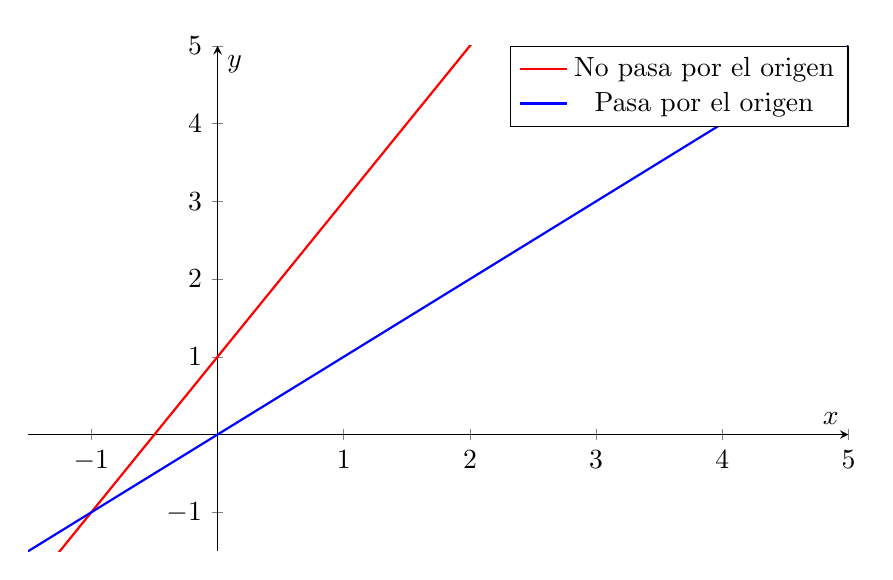
\begin{tikzpicture}
                    \begin{axis}
                        [
                        axis lines=middle,
                        xlabel={$x$},
                        ylabel={$y$},
                        xmin=-1.5, xmax=5,
                        ymin=-1.5, ymax=5,
                        legend style={at={(1,1)}, anchor=north east},
                        width=12cm,
                        height=8cm,
                        ]

                        % Line with positive gradient (y = 2x + 1)
                        \addplot[domain=-5:5, red, thick] {2*x + 1};
                        \addlegendentry{No pasa por el origen}

                        % Line that passes through the origin (y = x)
                        \addplot[domain=-5:5, blue, thick] {x};
                        \addlegendentry{Pasa por el origen}
                    \end{axis}
                \end{tikzpicture}
                \caption{Gráfica de dos magnitudes directamente proporcionales}
            \end{figure}
            \item \negsubro{Inversamente proporcional}
            Son gráficas en forma de curva como \( y = \dfrac{1}{x} \).

            \begin{remark}
                En este tipo de gráfica, si una magnitud aumenta, la otra debe disminuir.
            \end{remark}

            \begin{figure}[H]
                \centering
                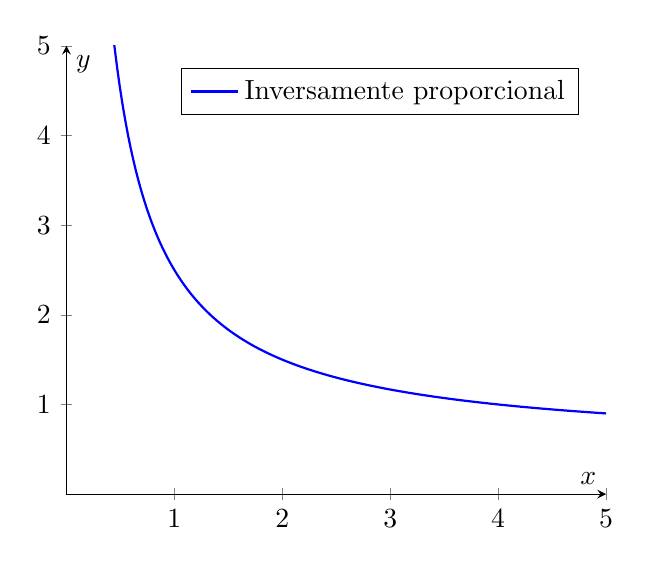
\begin{tikzpicture}
                    \begin{axis}
                        [
                        xlabel={$x$},
                        ylabel={$y$},
                        axis lines=middle,
                        ymin=0, ymax=5,
                        xmin=0, xmax=5,
                        samples=200,
                        domain=0.1:5, % Only the positive side
                        legend style={at={(0.95,0.95)}, anchor=north east},
                        legend entries={Inversamente proporcional}
                        ]
                        \addplot [blue, thick] {0.5 + 2/x};
                    \end{axis}
                \end{tikzpicture}
                \caption{Gráfica de dos magnitudes inversamente proporcionales}
            \end{figure}
        \end{itemize}
\end{enumerate}


\section{Magnitudes Físicas y sus Unidades}

\begin{definition}[Magnitud física]
        Es cualquier propiedad de un cuerpo que podemos medir.
        Por propiedad, entendemos una característica de un objeto.
\end{definition}
\vspace*{-8pt}
A toda magnitud, ya sea física o química, se le asigna una \textbf{unidad}.
\begin{definition}[Unidad]
        Una unidad es una cantidad definida por convenio para establecer un patrón.
\end{definition}
\vspace*{6pt}
Existen varios sistemas de unidades, pero el más utilizado es el Sistema Internacional de Unidades (SI).

Fue creado en 1960 por la Conferencia General de Pesas y Medidas y consta de 7 unidades básicas o fundamentales.

Gracias al sistema SI, se puede garantizar la fiabilidad de las especificaciones de los objetos en el comercio internacional.

Clasificamos las magnitudes en dos tipos:

\begin{itemize}
    \item \textbf{Magnitudes fundamentales}.
    Se definen por sí mismas; son las magnitudes básicas que no pueden descomponerse en otras magnitudes.

    En la Tabla \ref{tab:magnitudes_fundamentales}, se enumeran las magnitudes fundamentales, sus símbolos, las unidades del SI y los símbolos de las unidades.

    % Añade en el preámbulo: \usepackage{makecell}

    \begin{table}[H]
        \centering
        \caption{Magnitudes Fundamentales}
        \vspace{-5pt}
        \begin{tabular}{@{}lccc@{}}
            \toprule
            \textbf{Magnitud} & \makecell{\textbf{Símbolo de} \\ \textbf{la magnitud}}              & \textbf{Unidad}         & \makecell{\textbf{Símbolo de} \\ \textbf{la unidad}}                \\
            \midrule
            Longitud         & l         & metro   & \unit{\m} \\[3pt]
            Masa                & m         & kilogramo   & \unit{\kilo\g} \\[3pt]
            Temperatura    & T         & kelvin   & \unit{\kelvin} \\[3pt]
            Tiempo & t         & segundo     & \unit{\s} \\[3pt]
            Intensidad de corriente eléctrica  & I & amperio  & \unit{\ampere} \\[3pt]
            Cantidad de sustancia  & n & mol  & \unit{\mole} \\[3pt]
            Intensidad luminosa  & \( I_v \) & candela  & \unit{\candela} \\
            \bottomrule
        \end{tabular}
        \label{tab:magnitudes_fundamentales}
    \end{table}

%    \begin{table}[H]
%        \centering
%        \caption{Fundamental quantities}
%        \label{table:fundamental_quantities}
%        \begin{tblr}
%        {
%            colspec={|c|c|c|c|},
%            row{1} = {bg=darkblue!80, fg=white, font=\bfseries},
%            hlines,
%            vlines
%        }
%            Quantity & Quantity Symbol & Unit & Unit Symbol \\
%            Length & l & metre & \unit{\m} \\
%            Mass & m & kilogram & \unit{\kilo\g} \\
%            Temperature & T & kelvin & \unit{\kelvin} \\
%            Time & t & second & \unit{\s} \\
%            Electric current & I & ampere & \unit{\ampere} \\
%            Amount of substance & n & mole & \unit{\mole} \\
%            Luminous intensity & \( I_v \) & candela & \unit{\candela} \\
%        \end{tblr}
%    \end{table}


    \item \textbf{Magnitudes derivadas}.
    Se forman a partir de las magnitudes fundamentales y pueden expresarse como combinaciones de estas.

    La Tabla \ref{tab:derivative_quantities} enumera algunas magnitudes derivadas con sus unidades en el Sistema Internacional.

    \begin{table}[H]
        \centering
        \caption{Magnitudes Derivadas}
        \vspace{-5pt}
        \begin{tabular}{@{}lccc@{}}
            \toprule
            \textbf{Magnitud} & \makecell{\textbf{Símbolo de} \\ \textbf{la magnitud}}     & \textbf{Unidad}          & \makecell{\textbf{Símbolo de} \\ \textbf{la unidad}}   \\
            \midrule
            Área  & A & metro cuadrado           & \unit{\square\m} \\[3pt]
            Volumen    & V          & metro cúbico           & \unit{\cubic\m} \\[3pt]
            Densidad    & \( \rho \)          & --       & \unit{\kilo\g\per\cubic\m} \\[3pt]
            Velocidad & v          & --       & \unit{\mps} \\[3pt]
            Fuerza   & F          & newton        & \unit{\newton} \\[3pt]
            Presión   & p          & pascal        & \unit{\pascal} \\[3pt]
            Energía   & E          & julio        & \unit{\joule} \\[3pt]
            \bottomrule
        \end{tabular}
        \label{tab:derivative_quantities}
    \end{table}

%    \begin{table}[H]
%        \centering
%        \caption{Derivative quantities}
%        \label{table:derivative_quantities}
%        \begin{tblr}{
%            colspec={|c|c|c|c|},
%            row{1} = {bg=darkblue!80, fg=white, font=\bfseries},
%            hlines,
%            vlines
%        }
%            Quantity & Quantity Symbol & Unit & Unit Symbol \\
%            Area & A & square metre & \unit{\square\m} \\
%            Volume & V & cubic metre & \unit{\cubic\m} \\
%            Density & \( \rho \) & -- & \unit{\kilo\g\per\cubic\m} \\
%            Speed & v & -- & \unit{\mps} \\
%            Force & F & newton & \unit{\newton} \\
%            Pressure & p & pascal & \unit{\pascal} \\
%            Energy & E & joule & \unit{\joule} \\
%        \end{tblr}
%    \end{table}
\end{itemize}

\begin{remark}
    Si queremos determinar si una magnitud es fundamental o derivada, el método más sencillo es aprenderse las fundamentales.
    Si no es fundamental, entonces es derivada.
\end{remark}

\begin{exercise}
    En tu cuaderno, indica cuáles de las siguientes magnitudes son fundamentales y cuáles son derivadas:
    \vspace*{-12pt}
    \begin{multicols}{3}
        \begin{enumerate}[label=\letraminuscula]
            \item Intensidad de corriente eléctrica.
            \item Presión.
            \item Velocidad.
            \item Masa.
            \item Temperatura.
            \item Densidad.
            \item Energía.
            \item Longitud.
            \item Cantidad de sustancia
        \end{enumerate}
    \end{multicols}
    \begin{solu}
        En tu cuaderno, indica cuáles de las siguientes magnitudes son fundamentales y cuáles son derivadas:
        \begin{multicols}{2}
            \begin{enumerate}[label=\letraminuscula]
            \item Intensidad de corriente eléctrica. \textcolor{ocre}{Derivada}
            \item Presión. \textcolor{ocre}{Derivada}
            \item Velocidad. \textcolor{ocre}{Derivada}
            \item Masa. \textcolor{ocre}{Fundamental}
            \item Temperatura. \textcolor{ocre}{Fundamental}
            \item Densidad. \textcolor{ocre}{Derivada}
            \item Energía.\textcolor{ocre}{Derivada}
            \item Longitud. \textcolor{ocre}{Fundamental}
            \end{enumerate}
        \end{multicols}
    \end{solu}
\end{exercise}

\subsection{Múltiplos y Submúltiplos}

Al definir un sistema de unidades, también es necesario establecer los múltiplos y submúltiplos de dichas unidades, que nos permiten trabajar con cantidades numéricas más manejables.

La siguiente tabla muestra la relación entre una unidad y los distintos factores de proporcionalidad correspondientes a sus múltiplos y submúltiplos.
\begin{multicols}{2}
    \begin{table}[H]
        \centering
        \caption{Múltiplos}
        \vspace{-5pt}
        \begin{tabular}{@{}ccc@{}}
            \toprule
            \textbf{Orden de Magnitud} & \textbf{Nombre} & \textbf{Símbolo} \\
            \midrule
            \num{e12}                   & tera-         & T     \\[3pt]
            \num{e9}                    & giga-         & G               \\[3pt]
            \num{e6}                    & mega-         & M               \\[3pt]
            \num{e3}                    & kilo-         & k               \\[3pt]
            \num{e2}                    & hecto-        & h               \\[3pt]
            \num{10}                    & deca-         & da              \\[3pt]
            \bottomrule
            \multicolumn{3}{c}{\textbf{Unidad Base} }
            \\
            \bottomrule
        \end{tabular}
        \label{tab:Multiples}
    \end{table}
%    \begin{table}[H]
%        \caption{Multiples}
%        \label{table:Multiples}
%        \begin{tblr}{
%            colspec={|c|c|c|},
%            row{1} = {bg=darkblue!80, fg=white, font=\bfseries},
%            hlines,
%            vlines
%        }
%            Order of Magnitude & Name  & Symbol \\
%            \num{e12} & tera- & T \\
%            \num{e9} & giga- & G \\
%            \num{e6} & mega- & M \\
%            \num{e3} & kilo- & k \\
%            \num{e2} & hecto- & h \\
%            \num{10} & deca- & da \\
%            \SetRow{darkblue!70}\SetCell[c=3]{c} \textbf{\textcolor{white}{Base Unit}}
%        \end{tblr}
%    \end{table}
    \columnbreak
    \begin{table}[H]
        \centering
        \caption{Submúltiplos}
        \vspace{-5pt}
        \begin{tabular}{@{}ccc@{}}
            \toprule
            \textbf{Orden de Magnitud} & \textbf{Nombre} & \textbf{Símbolo} \\
            \toprule
            \multicolumn{3}{c}{\textbf{Unidad Base} } \\
            \toprule
            \num{e-1}                   & deci-         & d \\[3pt]
            \num{e-2}                   & centi-        & c \\[3pt]
            \num{e-3}                   & mili-        & m \\[3pt]
            \num{e-6}                   & micro-        & \( \mu \) \\[3pt]
            \num{e-9}                   & nano-         & n \\[3pt]
            \num{e-12}                  & pico-         & p               \\
            \bottomrule
        \end{tabular}
        \label{tab:Submultiples}
    \end{table}
%    \begin{table}[H]
%        \caption{Submultiples}
%        \label{table:Submultiples}
%
%        \begin{tblr}{
%            colspec={|c|c|c|},
%            row{1} = {bg=darkblue!80, fg=white, font=\bfseries},
%            hlines,
%            vlines
%        }
%            Order of Magnitude & Name  & Symbol \\
%            \SetRow{darkblue!70}\SetCell[c=3]{c} \textbf{\textcolor{white}{Base Unit}} \\
%            \num{e-1} & deci- & d \\
%            \num{e-2} & centi- & c \\
%            \num{e-3} & milli- & m \\
%            \num{e-6} & micro- & \( \mu \) \\
%            \num{e-9} & nano- & n \\
%            \num{e-12} & pico- & p \\
%        \end{tblr}
%    \end{table}
\end{multicols}

Las unidades del SI no son las únicas en uso; de hecho, casi todas las magnitudes tienen varias unidades posibles.
La siguiente tabla muestra magnitudes con distintas unidades y sus equivalencias con otras unidades de la misma magnitud.

\begin{table}[H]
    \centering
    \caption{Magnitudes con sus equivalencias}
    \vspace{-5pt}
    \begin{tabular}{@{}ccc@{}}
        \toprule
        \textbf{Magnitud}         & \textbf{Unidad}                   & \textbf{Equivalencia de la unidad}                           \\
        \midrule
        \multirow{3}{*}{Volumen}   & \unit{\kilo\litre}              & \qty{1}{\kilo\litre} = \qty{1}{\cubic\metre}        \\[3pt]
        & \unit{\litre}                   & \qty{1}{\litre} = \qty{1}{\cubic\deci\metre}        \\[3pt]
        & \unit{\milli\litre}             & \qty{1}{\milli\litre} = \qty{1}{\cubic\centi\metre} \\[3pt]
        \midrule
        \multirow{3}{*}{Presión} & Atmósfera (\unit{\atmosphere}) & \qty{1}{\atmosphere} = \qty{e5}{\pascal} \\[3pt]
        & \makecell{milímetro de mercurio \\  (\unit{\mmHg})}                    & \qty{1}{\atmosphere} = \qty{760}{\mmHg} \\[3pt]
        \midrule
        Energía                     & Caloría (\unit{\cal})           & \qty{1}{\cal} = \qty{4.18}{\joule}                   \\[3pt]
        \midrule
        Fuerza                     & Kilopondio (\unit{\kp})           & \qty{1}{\kp} = \qty{9.8}{\newton}                   \\
        \bottomrule
    \end{tabular}
    \label{tab:quantities_with_their_equivalences}
\end{table}

%\begin{table}[H]
%    \centering
%    \caption{Quantities with their equivalences}
%    \label{table:quantities_with_their_equivalences}
%    \begin{tblr}{
%        colspec={|c|c|c|},
%        row{1} = {bg=darkblue!80, fg=white, font=\bfseries},
%        hlines,
%        vlines,
%        cell{2}{1}={r=3}{c},
%        cell{5}{1}={r=2}{c},
%        rowhead=1
%    }
%        Quantity & Unit & Unit Equivalence \\
%        Volume & \unit{\kilo\litre} & \qty{1}{\kilo\litre} = \qty{1}{\cubic\metre} \\
%        & \unit{\litre} & \qty{1}{\litre} = \qty{1}{\cubic\deci\metre} \\
%        & \unit{\milli\litre} & \qty{1}{\milli\litre} = \qty{1}{\cubic\centi\metre} \\
%        Pressure & {Atmosphere \\ (\unit{\atmosphere})} & \qty{1}{\atmosphere} = \qty{e5}{\pascal} \\
%        & {millimetre of mercury \\ (\unit{\mmHg})} & \qty{1}{\atmosphere} = \qty{760}{\mmHg} \\
%        Energy & Calorie (\unit{\cal}) & \qty{1}{\cal} = \qty{4.18}{\joule} \\
%        Force & Kilopond (\unit{\kp}) & \qty{1}{\kp} = \qty{9.8}{\newton} \\
%    \end{tblr}
%\end{table}

\subsection{Conversión de Unidades Mediante Factores de Conversión}

Primero debemos tener en cuenta lo siguiente:
\begin{enumerate}[label=\letraminuscula]
        \item Podemos convertir entre unidades siempre que pertenezcan a la misma magnitud.
        \item Podemos convertir entre unidades con distintos múltiplos y submúltiplos.
        \item También podemos convertir entre distintas unidades siempre que representen la misma magnitud y conozcamos la equivalencia entre ellas.
\end{enumerate}

\begin{example}
    Convirtamos \qty{36}{\kmph} a \unit{\mps}:
    \begin{equation*}
        36\ \dfrac{\cancelred{\unit{\kilo\metre}}}{\cancel{\unit{\hour}}} \cdot \dfrac{1000\ \unit{\metre}}{1\ \cancelred{\unit{\kilo\metre}}} \cdot \dfrac{1\ \cancelred{\unit{\hour}}}{3600\ \unit{\second}} = \dfrac{36 \cdot 1000}{3600} = \qty{10}{\mps}
    \end{equation*}
\end{example}

\begin{example}
    Convierte \qty{13600}{\kilo\g\per\cubic\metre} a \unit{\g\per\cubic\centi\metre}:
    \begin{equation*}
        13600\ \dfrac{\cancelred{\unit{\kilo\g}}}{\cancel{\unit{\cubic\metre}}} \cdot \dfrac{1000\ \unit{\g}}{1\ \cancelred{\unit{\kilo\g}}} \cdot \dfrac{1\ \cancelred{\unit{\cubic\metre}}}{\num{e6}\ \unit{\cubic\centi\metre}} = \dfrac{13600 \cdot 1000}{\num{e6}} = \qty{13.6}{\g\per\cubic\centi\metre}
    \end{equation*}
\end{example}

\begin{example}
    Convierte \qty{12}{\kilo\metre} a \unit{\nano\metre}:
    \begin{equation*}
        12\ \cancelred{\unit{\kilo\metre}} \cdot  \dfrac{\num{e12}\ \unit{\nano\metre}}{ 1\ \cancelred{\unit{\kilo\metre}}} = \num{12e-12} = \qty{1.2e-11}{\nano\metre}
    \end{equation*}
\end{example}

\begin{exercise}
    Convierte las siguientes velocidades a las unidades indicadas utilizando factores de conversión.
    \begin{enumerate}[label=\letraminuscula]
        \item Convierte las siguientes velocidades a \unit{\mps}:
        \begin{multicols}{4}
            \begin{itemize}
                \item \qty{90}{\kmph}
                \item \qty{100}{\kmph}
                \item \qty{120}{\kmph}
                \item \qty{50}{\kmph}
            \end{itemize}
        \end{multicols}
        \item Convierte las siguientes velocidades a \unit{\kmph}:
        \begin{multicols}{4}
            \begin{itemize}
                \item \qty{12}{\mps}
                \item \qty{340}{\mps}
                \item \qty{0.36}{\mps}
                \item \qty{3e8}{\mps}
            \end{itemize}
        \end{multicols}
    \end{enumerate}
    \begin{solu}

        Para realizar estas conversiones, utilizamos las siguientes relaciones de equivalencia: $1 \text{ km} = 1000 \text{ m}$ y $1 \text{ h} = 3600 \text{ s}$.

        \textbf{a) Conversión de km/h a m/s:}
        \begin{itemize}
            \item \textbf{90 km/h}:
            \[ 90 \frac{\cancel{\text{km}}}{\cancel{\text{h}}} \cdot \frac{1000 \text{ m}}{1 \cancel{\text{km}}} \cdot \frac{1 \cancel{\text{h}}}{3600 \text{ s}} = \frac{90 \cdot 1000}{3600} \text{ m/s} = 25 \text{ m/s} \]

            \item \textbf{100 km/h}:
            \[ 100 \frac{\cancel{\text{km}}}{\cancel{\text{h}}} \cdot \frac{1000 \text{ m}}{1 \cancel{\text{km}}} \cdot \frac{1 \cancel{\text{h}}}{3600 \text{ s}} = \frac{100000}{3600} \text{ m/s} \approx 27.78 \text{ m/s} \]

            \item \textbf{120 km/h}:
            \[ 120 \frac{\cancel{\text{km}}}{\cancel{\text{h}}} \cdot \frac{1000 \text{ m}}{1 \cancel{\text{km}}} \cdot \frac{1 \cancel{\text{h}}}{3600 \text{ s}} = \frac{120000}{3600} \text{ m/s} \approx 33.33 \text{ m/s} \]

            \item \textbf{50 km/h}:
            \[ 50 \frac{\cancel{\text{km}}}{\cancel{\text{h}}} \cdot \frac{1000 \text{ m}}{1 \cancel{\text{km}}} \cdot \frac{1 \cancel{\text{h}}}{3600 \text{ s}} = \frac{50000}{3600} \text{ m/s} \approx 13.89 \text{ m/s} \]
        \end{itemize}

        \textbf{b) Conversión de m/s a km/h:}
        \begin{itemize}
            \item \textbf{12 m/s}:
            \[ 12 \frac{\cancel{\text{m}}}{\cancel{\text{s}}} \cdot \frac{1 \text{ km}}{1000 \cancel{\text{m}}} \cdot \frac{3600 \cancel{\text{s}}}{1 \text{ h}} = 12 \cdot 3.6 \text{ km/h} = 43.2 \text{ km/h} \]

            \item \textbf{340 m/s}:
            \[ 340 \frac{\cancel{\text{m}}}{\cancel{\text{s}}} \cdot \frac{1 \text{ km}}{1000 \cancel{\text{m}}} \cdot \frac{3600 \cancel{\text{s}}}{1 \text{ h}} = 340 \cdot 3.6 \text{ km/h} = 1224 \text{ km/h} \]

            \item \textbf{0.36 m/s}:
            \[ 0.36 \frac{\cancel{\text{m}}}{\cancel{\text{s}}} \cdot \frac{1 \text{ km}}{1000 \cancel{\text{m}}} \cdot \frac{3600 \cancel{\text{s}}}{1 \text{ h}} = 0.36 \cdot 3.6 \text{ km/h} = 1.296 \text{ km/h} \]

            \item \textbf{$3 \cdot 10^8$ m/s}:
            \[ 3 \cdot 10^8 \frac{\cancel{\text{m}}}{\cancel{\text{s}}} \cdot \frac{1 \text{ km}}{1000 \cancel{\text{m}}} \cdot \frac{3600 \cancel{\text{s}}}{1 \text{ h}} = 3 \cdot 10^8 \cdot 3.6 \text{ km/h} = 1.08 \cdot 10^9 \text{ km/h} \]
        \end{itemize}
    \end{solu}
\end{exercise}


\begin{exercise}
    Convierte las siguientes unidades a las unidades del SI correspondientes utilizando factores de conversión.
    \begin{multicols}{4}
        \begin{enumerate}[label=\letraminuscula]
            \item \qty{200}{\square\centi\metre}
            \item \qty{125}{\cubic\centi\metre}
            \item \qty{1800}{\g}
            \item \qty{45}{\min}
        \end{enumerate}
    \end{multicols}


    \begin{solu}
        Para convertir estos valores al Sistema Internacional de Unidades (SI), utilizamos las unidades básicas: metros (\unit{\m}), kilogramos (\unit{\kg}) y segundos (\unit{\s}).

        \textbf{a) Conversión de área (\unit{\square\centi\metre} a \unit{\square\metre}):}
        Dado que \( \qty{1}{\metre} = \qty{100}{\centi\metre} \), entonces \( \qty{1}{\square\metre} = (\qty{100}{\centi\metre})^2 = \qty{10000}{\square\centi\metre} \).
        \[ \qty{200}{\cancel{\square\centi\metre}} \cdot \frac{\qty{1}{\square\metre}}{\qty{10000}{\cancel{\square\centi\metre}}} = \qty{0.02}{\square\metre} \]

        \textbf{b) Conversión de volumen (\unit{\cubic\centi\metre} a \unit{\cubic\metre}):}
        Dado que \( \qty{1}{\metre} = \qty{100}{\centi\metre} \), entonces \( \qty{1}{\cubic\metre} = (\qty{100}{\centi\metre})^3 = \qty{1000000}{\cubic\centi\metre} \).
        \[ \qty{125}{\cancel{\cubic\centi\metre}} \cdot \frac{\qty{1}{\cubic\metre}}{\qty{1000000}{\cancel{\cubic\centi\metre}}} = \qty{1.25e-4}{\cubic\metre} \]

        \textbf{c) Conversión de masa (\unit{\g} a \unit{\kg}):}
        Equivalencia: \( \qty{1}{\kg} = \qty{1000}{\g} \).
        \[ \qty{1800}{\cancel{\g}} \cdot \frac{\qty{1}{\kg}}{\qty{1000}{\cancel{\g}}} = \qty{1.8}{\kg} \]

        \textbf{d) Conversión de tiempo (\unit{\min} a \unit{\s}):}
        Equivalencia: \( \qty{1}{\min} = \qty{60}{\s} \).
        \[ \qty{45}{\cancel{\min}} \cdot \frac{\qty{60}{\s}}{\qty{1}{\cancel{\min}}} = \qty{2700}{\s} \]
    \end{solu}

\end{exercise}

\begin{exercise}
    Realiza las siguientes conversiones de unidades a unidades del SI utilizando factores de conversión
    \begin{multicols}{4}
        \begin{enumerate}[label=\letraminuscula]
\item \qty{300}{\mmHg}
\item \qty{25000}{\cal}
\item \qty{21}{\atmosphere}
\item \qty{258}{\kilopondio}
        \end{enumerate}
    \end{multicols}


    \begin{solu}
        En el Sistema Internacional, la unidad derivada de la presión es el Pascal (\unit{\Pa}), la de la energía es el Julio (\unit{\J}) y la de la fuerza es el Newton (\unit{\N}).

        \textbf{a) Presión (\unit{\mmHg} a \unit{\Pa}):}
        Equivalencia: \( \qty{760}{\mmHg} = \qty{101325}{\Pa} \).
        \[ \qty{300}{\cancel{\mmHg}} \cdot \frac{\qty{101325}{\Pa}}{\qty{760}{\cancel{\mmHg}}} \approx \qty{39996.71}{\Pa} \]

        \textbf{b) Energía (\unit{cal} a \unit{\J}):}
        Equivalencia: \( \qty{1}{cal} = \qty{4.184}{\J} \).
        \[ \qty{25000}{\cancel{cal}} \cdot \frac{\qty{4.184}{\J}}{\qty{1}{\cancel{cal}}} = \qty{104600}{\J} \]

        \textbf{c) Presión (\unit{atm} a \unit{\Pa}):}
        Equivalencia: \( \qty{1}{atm} = \qty{101325}{\Pa} \).
        \[ \qty{21}{\cancel{atm}} \cdot \frac{\qty{101325}{\Pa}}{\qty{1}{\cancel{atm}}} = \qty{2127825}{\Pa} \]

        \textbf{d) Fuerza (\unit{kp} a \unit{\N}):}
        Equivalencia: \( \qty{1}{kp} = \qty{9.8}{\N} \).
        \[ \qty{258}{\cancel{kp}} \cdot \frac{\qty{9.8}{\N}}{\qty{1}{\cancel{kp}}} = \qty{2528.4}{\N} \]
    \end{solu}

\end{exercise}

\begin{exercise}
    Si 1 g de oro puro cuesta 31,32 €, calcula el precio de 1 dg y 1 cg de este metal. Resuelve el siguiente ejercicio utilizando factores de conversión.

    \begin{solu}
        Usando las relaciones de masa dentro del sistema decimal: \( \qty{1}{\g} = \qty{10}{\deci\g} \) y \( \qty{1}{\g} = \qty{100}{\centi\g} \).

        \textbf{1) Precio de \qty{1}{\deci\g}:}
        \[ \qty{1}{\cancel{\deci\g}} \cdot \frac{\qty{1}{\cancel{\g}}}{\qty{10}{\cancel{\deci\g}}} \cdot \frac{\text{31.32 €}}{\qty{1}{\cancel{\g}}} = \text{3.13 €} \]

        \textbf{2) Precio de \qty{1}{\centi\g}:}
        \[ \qty{1}{\cancel{\centi\g}} \cdot \frac{\qty{1}{\cancel{\g}}}{\qty{100}{\cancel{\centi\g}}} \cdot \frac{\text{31.32 €}}{\qty{1}{\cancel{\g}}} = \text{0.31 €} \]
    \end{solu}

\end{exercise}

\begin{exercise}
    Si 1 kg de almendras cuesta 18,40 €, calcula el precio de 1 hg y 1 dag de este producto. Resuelve el siguiente ejercicio utilizando factores de conversión.

    \begin{solu}
        Usando las relaciones de masa dentro del sistema decimal: \( \qty{1}{\kg} = \qty{10}{\hecto\g} \) y \( \qty{1}{\kg} = \qty{100}{\deca\g} \).

        \textbf{1) Precio de \qty{1}{\hecto\g}:}
        \[
        \qty{1}{\cancel{\hecto\g}} \cdot
        \frac{\qty{1}{\cancel{\kg}}}{\qty{10}{\cancel{\hecto\g}}} \cdot
        \frac{\text{18.40 €}}{\qty{1}{\cancel{\kg}}}
        = \text{1.84 €}
        \]

        \textbf{2) Precio de \qty{1}{\deca\g}:}
        \[
        \qty{1}{\cancel{\deca\g}} \cdot
        \frac{\qty{1}{\cancel{\kg}}}{\qty{100}{\cancel{\deca\g}}} \cdot
        \frac{\text{18.40 €}}{\qty{1}{\cancel{\kg}}}
        = \text{0.184 €}
        \]
    \end{solu}

\end{exercise}

\begin{exercise}
    Si 1 L de aceite de oliva cuesta 9,60 €, calcula el precio de 1 dL y 1 cL de este líquido. Resuelve el siguiente ejercicio utilizando factores de conversión.

    \begin{solu}
        Usando las relaciones de capacidad dentro del sistema decimal: \( \qty{1}{\L} = \qty{10}{\deci\L} \) y \( \qty{1}{\L} = \qty{100}{\centi\L} \).

        \textbf{1) Precio de \qty{1}{\deci\L}:}
        \[
        \qty{1}{\cancel{\deci\L}} \cdot
        \frac{\qty{1}{\cancel{\L}}}{\qty{10}{\cancel{\deci\L}}} \cdot
        \frac{\text{9.60 €}}{\qty{1}{\cancel{\L}}}
        = \text{0.96 €}
        \]

        \textbf{2) Precio de \qty{1}{\centi\L}:}
        \[
        \qty{1}{\cancel{\centi\L}} \cdot
        \frac{\qty{1}{\cancel{\L}}}{\qty{100}{\cancel{\centi\L}}} \cdot
        \frac{\text{9.60 €}}{\qty{1}{\cancel{\L}}}
        = \text{0.096 €}
        \]
    \end{solu}

\end{exercise}


\section{Notación Científica}

La notación científica nos permite escribir números muy grandes o muy pequeños utilizando potencias de \num{10}, con un exponente positivo para números muy grandes o un exponente negativo para números muy pequeños.

Para que un número esté correctamente expresado en notación científica, debe tener:

\begin{itemize}
    \item Un único dígito distinto de cero a la izquierda de la coma decimal.
    \item Una potencia de 10 elevada a un exponente positivo o negativo.
\end{itemize}

Por ejemplo:

\begin{itemize}
    \item La masa de la Tierra es:

    \qty{6000000000000000000000000}{\kilo\g}.
    Como podemos ver, este número tiene 24 ceros, por lo que escribirlo repetidamente resulta bastante tedioso.
    Este número en notación científica sería: \qty{6e24}{\kilo\g}.

    \item La masa del electrón es:

    \qty{0.0000000000000000000000000000009109}{\kilo\g}.
    Este número en notación científica se escribe como \qty{9.3109e-31}{\kilo\g}.
\end{itemize}

Los pasos para convertir a notación científica son los siguientes:

\begin{itemize}
    \item \textbf{Números mayores que uno}.
    Comenzamos por la derecha del número.
    En ese punto, colocamos la coma decimal y contamos cuántas posiciones necesitamos desplazarla para que quede un único dígito distinto de cero a su izquierda.
    El número en notación científica será el nuevo número multiplicado por una potencia de 10, elevada al número de posiciones desplazadas, con exponente positivo.
    Por eso, en el caso anterior obtenemos \num{6e24}.

    \item \textbf{Números menores que uno}.
    Comenzamos por la coma decimal y contamos cuántas posiciones necesitamos desplazarla para que quede un único dígito distinto de cero a su izquierda.
    El exponente resultante será negativo.

    \item \textbf{Números que ya son grandes o pequeños pero que ya incluyen una potencia de 10} .
    Comenzamos por la coma decimal.
    Pueden darse los siguientes casos:

    \begin{itemize}
        \item Si el número es mayor que uno:
        Procedemos como en el caso anterior, y el número de posiciones se \emph{suma} al exponente de la potencia decimal. Ejemplos:
        \begin{itemize}
            \item \num{625.5e5} se convierte en \num{6.255e7}.
            \item \num{45654.21e-2} se convierte en \num{4.5654e-2}.
        \end{itemize}

        \item Si el número es menor que uno:
        Procedemos de forma similar, pero en este caso el número de posiciones se \emph{resta} del exponente. Ejemplos:
        \begin{itemize}
            \item \num{0.0523e-3} se convierte en \num{5.23e-5}.
            \item \num{0.000254e5} se convierte en \num{2.54e-1}.
        \end{itemize}
    \end{itemize}
\end{itemize}

\begin{exercise}
    Escribe las siguientes cantidades en notación científica:
    \begin{multicols}{3}
        \begin{enumerate}[label=\letraminuscula]
\item \qty{20000000}{\m}
\item \qty{250000000}{\litre}
\item \qty{7820000000}{\g}
\item \qty{254830368}{\km}
\item \qty{0.0001}{\s}
\item \qty{0.000035}{\kilo\g}
\item \qty{0.000001}{\m}
\item \qty{0.000005001}{\g}
\item \qty{0.000000005}{\g}
        \end{enumerate}
    \end{multicols}

    \begin{solu}
        Para escribir en notación científica, desplazamos la coma decimal para obtener un número entre 1 y 10, y luego multiplicamos por la potencia de 10 correspondiente.
        \begin{itemize}
            \item \textbf{a)} \( \qty{20000000}{\m} = \qty{2e7}{\m} \)
            \item \textbf{b)} \( \qty{250000000}{\litre} = \qty{2.5e8}{\litre} \)
            \item \textbf{c)} \( \qty{7820000000}{\g} = \qty{7.82e9}{\g} \)
            \item \textbf{d)} \( \qty{254830368}{\km} \approx \qty{2.55e8}{\km} \)
            \item \textbf{e)} \( \qty{0.0001}{\s} = \qty{1e-4}{\s} \)
            \item \textbf{f)} \( \qty{0.000035}{\kg} = \qty{3.5e-5}{\kg} \)
            \item \textbf{g)} \( \qty{0.000001}{\m} = \qty{1e-6}{\m} \)
            \item \textbf{h)} \( \qty{0.000005001}{\g} = \qty{5.001e-6}{\g} \)
            \item \textbf{i)} \( \qty{0.000000005}{\g} = \qty{5e-9}{\g} \)
        \end{itemize}
    \end{solu}

\end{exercise}
\begin{exercise}
    Escribe las siguientes cantidades en notación científica.
    \begin{multicols}{3}
        \begin{enumerate}[label=\letraminuscula]
\item \qty{0.00005}{\g}
\item \qty{0.000052}{\g}
\item \qty{2000000}{\m}
\item \qty{25000000}{\m}
\item \qty{301000}{\s}
\item \qty{0.000205}{\ampere}
\item \qty{20520000000}{\kg}
\item \qty{5000000000}{\kg}
        \end{enumerate}
    \end{multicols}

    \begin{solu}
        \begin{itemize}
            \item \textbf{a)} \( \qty{0.00005}{\g} = \qty{5e-5}{\g} \)
            \item \textbf{b)} \( \qty{0.000052}{\g} = \qty{5.2e-5}{\g} \)
            \item \textbf{c)} \( \qty{2000000}{\m} = \qty{2e6}{\m} \)
            \item \textbf{d)} \( \qty{25000000}{\m} = \qty{2.5e7}{\m} \)
            \item \textbf{e)} \( \qty{301000}{\s} = \qty{3.01e5}{\s} \)
            \item \textbf{f)} \( \qty{0.000205}{\ampere} = \qty{2.05e-4}{\ampere} \)
            \item \textbf{g)} \( \qty{20520000000}{\kg} = \qty{2.052e10}{\kg} \)
            \item \textbf{h)} \( \qty{5000000000}{\kg} = \qty{5e9}{\kg} \)
        \end{itemize}
    \end{solu}

\end{exercise}

\begin{exercise}
    Expresa las siguientes medidas en unidades del SI utilizando factores de conversión y notación científica.
    \begin{multicols}{4}
        \begin{enumerate}[label=\letraminuscula]
\item \qty{0.5}{\g}
\item \qty{0.5}{\cubic\centi\metre}
\item \qty{200}{\square\kilo\metre}
\item \qty{2}{\g\per\cubic\centi\metre}
\item \qty{76}{\hecto\m}
\item \qty{3}{\milli\g}
\item \qty{9}{\deca\m}
\item \qty{25}{\nano\s}
        \end{enumerate}
    \end{multicols}

    \begin{solu}
        \begin{itemize}
            \item \textbf{a) \qty{0.5}{\g} a \unit{\kg}:}
            \[ \qty{0.5}{\cancel{\g}} \cdot \frac{\qty{1}{\kg}}{\qty{1000}{\cancel{\g}}} = \qty{5e-4}{\kg} \]
            \item \textbf{b) \qty{0.5}{\cubic\centi\metre} a \unit{\cubic\metre}:}
            \[ \qty{0.5}{\cancel{\cubic\centi\metre}} \cdot \frac{\qty{1}{\cubic\metre}}{\qty{1e6}{\cancel{\cubic\centi\metre}}} = \qty{5e-7}{\cubic\metre} \]
            \item \textbf{c) \qty{200}{\square\kilo\metre} a \unit{\square\metre}:}
            \[ \qty{200}{\cancel{\square\kilo\metre}} \cdot \frac{\qty{1e6}{\square\metre}}{\qty{1}{\cancel{\square\kilo\metre}}} = \qty{2e8}{\square\metre} \]
            \item \textbf{d) \qty{2}{\g\per\cubic\centi\metre} a \unit{\kg\per\cubic\metre}:}
            \[ \frac{\qty{2}{\cancel{\g}}}{\qty{1}{\cancel{\cubic\centi\metre}}} \cdot \frac{\qty{1}{\kg}}{\qty{1000}{\cancel{\g}}} \cdot \frac{\qty{1e6}{\cancel{\cubic\centi\metre}}}{\qty{1}{\cubic\metre}} = \qty{2e3}{\kg\per\cubic\metre} \]
            \item \textbf{e) \qty{76}{\hecto\m} a \unit{\m}:}
            \[ \qty{76}{\cancel{\hecto\m}} \cdot \frac{\qty{100}{\m}}{\qty{1}{\cancel{\hecto\m}}} = \qty{7.6e3}{\m} \]
            \item \textbf{f) \qty{3}{\milli\g} a \unit{\kg}:}
            \[ \qty{3}{\cancel{\milli\g}} \cdot \frac{\qty{1}{\kg}}{\qty{1e6}{\cancel{\milli\g}}} = \qty{3e-6}{\kg} \]
            \item \textbf{g) \qty{9}{\deca\m} a \unit{\m}:}
            \[ \qty{9}{\cancel{\deca\m}} \cdot \frac{\qty{10}{\m}}{\qty{1}{\cancel{\deca\m}}} = \qty{9e1}{\m} \]
            \item \textbf{h) \qty{25}{\nano\s} a \unit{\s}:}
            \[ \qty{25}{\cancel{\nano\s}} \cdot \frac{\qty{1}{\s}}{\qty{1e9}{\cancel{\nano\s}}} = \qty{2.5e-8}{\s} \]
        \end{itemize}
    \end{solu}

\end{exercise}

\begin{exercise}
    Expresa los siguientes volúmenes en unidades del SI utilizando factores de conversión y notación científica:
    \begin{multicols}{4}
        \begin{enumerate}[label=\letraminuscula]
\item \qty{0.5}{\mL}
\item \qty{0.001}{\mL}
\item \qty{33.3}{\kL}
\item \qty{10000}{\litre}
        \end{enumerate}
    \end{multicols}


    \begin{solu}
        Recuerda que, para el volumen, el \unit{\cubic\metre} es la unidad del SI y \( \qty{1}{\litre} = \qty{1}{\cubic\deci\metre} \). Por lo tanto, \( \qty{1000}{\litre} = \qty{1}{\cubic\metre} \).
        \begin{itemize}
            \item \textbf{a) \qty{0.5}{\mL} a \unit{\cubic\metre}:}
            \[ \qty{0.5}{\cancel{\mL}} \cdot \frac{\qty{1}{\cancel{\litre}}}{\qty{1000}{\cancel{\mL}}} \cdot \frac{\qty{1}{\cubic\metre}}{\qty{1000}{\cancel{\litre}}} = \qty{5e-7}{\cubic\metre} \]
            \item \textbf{b) \qty{0.001}{\mL} a \unit{\cubic\metre}:}
            \[ \qty{0.001}{\cancel{\mL}} \cdot \frac{\qty{1}{\cancel{\litre}}}{\qty{1000}{\cancel{\mL}}} \cdot \frac{\qty{1}{\cubic\metre}}{\qty{1000}{\cancel{\litre}}} = \qty{1e-9}{\cubic\metre} \]
            \item \textbf{c) \qty{33.3}{\kL} a \unit{\cubic\metre}:}
            \[ \qty{33.3}{\cancel{\kL}} \cdot \frac{\qty{1000}{\cancel{\litre}}}{\qty{1}{\cancel{\kL}}} \cdot \frac{\qty{1}{\cubic\metre}}{\qty{1000}{\cancel{\litre}}} = \qty{3.33e1}{\cubic\metre} \]
            \item \textbf{d) \qty{10000}{\litre} a \unit{\cubic\metre}:}
            \[ \qty{10000}{\cancel{\litre}} \cdot \frac{\qty{1}{\cubic\metre}}{\qty{1000}{\cancel{\litre}}} = \qty{1e1}{\cubic\metre} \]
        \end{itemize}
    \end{solu}

\end{exercise}

\begin{exercise}
    Elabora un mapa conceptual de la unidad.

    \begin{solu}
        Un mapa conceptual para "Unidades y Medidas" debería incluir:
        \begin{itemize}
            \item \textbf{Magnitudes físicas:} Fundamentales (masa, longitud, tiempo) y Derivadas (velocidad, densidad, volumen).
            \item \textbf{Sistema Internacional (SI):} Unidades estándar como \unit{\kg}, \unit{\m}, \unit{\s}.
            \item \textbf{Instrumentos de medida:} Precisión, exactitud y sensibilidad.
            \item \textbf{Notación científica:} Expresar números muy grandes o muy pequeños mediante potencias de 10.
            \item \textbf{Conversión de unidades:} Uso de factores de conversión y el sistema métrico (prefijos como kilo-, centi-, mili-).
        \end{itemize}
    \end{solu}

\end{exercise}


%\section{Vocabulario}
%
%\begin{vocabulary}[Scientific Method]
%A systematic approach used by scientists to investigate phenomena, acquire new knowledge, or correct and integrate previous knowledge. It involves observation, hypothesis formulation, experimentation, and analysis of results to develop laws, theories, or models. \newline
%\textbf{Translation to Spanish}: Método científico \newline
%% Line 5
%\end{vocabulary}
%
%\begin{vocabulary}[Observation]
%The first stage of the scientific method that involves carefully watching and recording phenomena or events in nature using the senses or instruments. \newline
%\textbf{Translation to Spanish}: Observación \newline
%% Line 9
%\end{vocabulary}
%
%\begin{vocabulary}[Hypothesis]
%A provisional assumption or proposed explanation made to explain a specific fact or phenomenon that can be tested through experimentation. \newline
%\textbf{Translation to Spanish}: Hipótesis \newline
%% Line 15
%\end{vocabulary}
%
%\begin{vocabulary}[Experimentation]
%The process of carrying out controlled experimental tests to verify or refute a hypothesis through systematic observation and measurement. \newline
%\textbf{Translation to Spanish}: Experimentación \newline
%% Line 16
%\end{vocabulary}
%
%\begin{vocabulary}[Law]
%A statement based on repeated experimental observations that describes some aspect of nature, always occurring under the same conditions. Laws are often expressed mathematically. \newline
%\textbf{Translation to Spanish}: Ley \newline
%% Line 21
%\end{vocabulary}
%
%\begin{vocabulary}[Theory]
%A well-substantiated explanation of some aspect of the natural world that is based on a body of facts that have been repeatedly confirmed through observation and experimentation. \newline
%\textbf{Translation to Spanish}: Teoría \newline
%% Line 21
%\end{vocabulary}
%
%\begin{vocabulary}[Model]
%A simplified representation of a system or phenomenon that helps explain and predict its behavior, often using mathematical equations, diagrams, or physical constructs. \newline
%\textbf{Translation to Spanish}: Modelo \newline
%% Line 21
%\end{vocabulary}
%
%\begin{vocabulary}[Variable]
%Any factor, trait, or condition that can exist in differing amounts or types in an experiment or observation. \newline
%\textbf{Translation to Spanish}: Variable \newline
%% Line 33
%\end{vocabulary}
%
%\begin{vocabulary}[Independent Variable]
%The variable that is deliberately changed or controlled in an experiment to test its effects on the dependent variable. It is plotted on the horizontal axis (X-axis). \newline
%\textbf{Translation to Spanish}: Variable independiente \newline
%% Line 35
%\end{vocabulary}
%
%\begin{vocabulary}[Dependent Variable]
%The variable that is measured or observed in an experiment. It depends on the independent variable and is plotted on the vertical axis (Y-axis). \newline
%\textbf{Translation to Spanish}: Variable dependiente \newline
%% Line 36
%\end{vocabulary}
%
%\begin{vocabulary}[Directly Proportional]
%A relationship between two quantities where if one quantity increases, the other also increases at a constant rate. Graphically represented by a straight line with equation y = mx + n. \newline
%\textbf{Translation to Spanish}: Directamente proporcional \newline
%% Line 61
%\end{vocabulary}
%
%\begin{vocabulary}[Inversely Proportional]
%A relationship between two quantities where if one quantity increases, the other decreases. Graphically represented by a hyperbolic curve of the form y = 1/x. \newline
%\textbf{Translation to Spanish}: Inversamente proporcional \newline
%% Line 96
%\end{vocabulary}
%
%\begin{vocabulary}[Gradient]
%The slope of a line in a graph, represented by the letter m in the equation y = mx + n. It indicates the rate of change of the dependent variable with respect to the independent variable. \newline
%\textbf{Translation to Spanish}: Pendiente \newline
%% Line 64
%\end{vocabulary}
%
%\begin{vocabulary}[Physical Quantity]
%Any property of a body or system that can be measured and expressed numerically with an appropriate unit. \newline
%\textbf{Translation to Spanish}: Magnitud física \newline
%% Line 129
%\end{vocabulary}
%
%\begin{vocabulary}[Unit]
%A quantity defined by convention to establish a standard for measurement. It provides a reference to express the value of physical quantities. \newline
%\textbf{Translation to Spanish}: Unidad \newline
%% Line 135
%\end{vocabulary}
%
%\begin{vocabulary}[International System of Units (SI)]
%The modern form of the metric system established in 1960 by the General Conference on Weights and Measures, consisting of 7 base units and derived units for measuring physical quantities. \newline
%\textbf{Translation to Spanish}: Sistema Internacional de Unidades \newline
%% Line 138
%\end{vocabulary}
%
%\begin{vocabulary}[Fundamental Quantities]
%Basic physical quantities that cannot be broken down into other quantities and are defined independently. Examples include length, mass, time, temperature, electric current, amount of substance, and luminous intensity. \newline
%\textbf{Translation to Spanish}: Magnitudes fundamentales \newline
%% Line 147
%\end{vocabulary}
%
%\begin{vocabulary}[Derived Quantities]
%Physical quantities that are defined in terms of combinations of fundamental quantities. Examples include area, volume, velocity, and density. \newline
%\textbf{Translation to Spanish}: Magnitudes derivadas \newline
%% Line 195 (approximately, based on context)
%\end{vocabulary}
%
%\begin{vocabulary}[Length]
%A fundamental quantity that measures the distance between two points. The SI unit is the metre (m). \newline
%\textbf{Translation to Spanish}: Longitud \newline
%% Line 162
%\end{vocabulary}
%
%\begin{vocabulary}[Mass]
%A fundamental quantity that measures the amount of matter in an object. The SI unit is the kilogram (kg). \newline
%\textbf{Translation to Spanish}: Masa \newline
%% Line 163
%\end{vocabulary}
%
%\begin{vocabulary}[Temperature]
%A fundamental quantity that measures the degree of hotness or coldness of a body. The SI unit is the kelvin (K). \newline
%\textbf{Translation to Spanish}: Temperatura \newline
%% Line 164
%\end{vocabulary}
%
%\begin{vocabulary}[Time]
%A fundamental quantity that measures the duration of events or the interval between them. The SI unit is the second (s). \newline
%\textbf{Translation to Spanish}: Tiempo \newline
%% Line 165
%\end{vocabulary}
%
%\begin{vocabulary}[Electric Current]
%A fundamental quantity that measures the flow of electric charge through a conductor. The SI unit is the ampere (A). \newline
%\textbf{Translation to Spanish}: Corriente eléctrica \newline
%% Line 166
%\end{vocabulary}
%
%\begin{vocabulary}[Amount of Substance]
%A fundamental quantity that measures the number of elementary entities (atoms, molecules, ions, etc.) in a sample. The SI unit is the mole (mol). \newline
%\textbf{Translation to Spanish}: Cantidad de sustancia \newline
%% Line 167
%\end{vocabulary}
%
%\begin{vocabulary}[Luminous Intensity]
%A fundamental quantity that measures the power emitted by a light source in a particular direction. The SI unit is the candela (cd). \newline
%\textbf{Translation to Spanish}: Intensidad luminosa \newline
%% Line 168
%\end{vocabulary}
%
%\begin{vocabulary}[Scientific Notation]
%A method of writing very large or very small numbers as a product of a number between 1 and 10 and a power of 10. It consists of a single non-zero digit to the left of the decimal point multiplied by 10 raised to an exponent. \newline
%\textbf{Translation to Spanish}: Notación científica \newline
%% Line 499
%\end{vocabulary}
%
%\begin{vocabulary}[Exponent]
%The power to which a base number (such as 10 in scientific notation) is raised. It can be positive for large numbers or negative for small numbers. \newline
%\textbf{Translation to Spanish}: Exponente \newline
%% Line 507
%\end{vocabulary}


\section{Ejercicios complementarios sobre conversión de unidades y notación científica}

\subsection{Notación Científica}

\begin{exercise}
    \phantom{a}
    \begin{enumerate}[label=\letraminuscula]
        \item \num{4569201}
        \item \num{0.0026}
        \item \num{235.78}
        \item \num{500000}
        \item \num{4055e4}
        \item \num{5687e-8}
        \item \num{253e8}
        \item \num{0.0254e-2}
    \end{enumerate}
\end{exercise}

\subsection{Unidades Fundamentales}

\begin{exercise}
    \phantom{a}
    \begin{enumerate}[label=\letraminuscula]
        \item \qty{500}{\hecto\g} a \unit{\g}
        \item \qty{60}{\centi\metre} a \unit{\metre}
        \item \qty{2000}{\hecto\metre} a \unit{\deca\metre}
        \item \qty{5.7}{\kilo\g} a \unit{\g}
        \item \qty{300}{\deci\metre} a \unit{\hecto\metre}
        \item \qty{563}{\kilo\metre} a \unit{\hecto\metre}
        \item \qty{3}{\deci\metre} a \unit{\deca\metre}
        \item \qty{7}{\deci\metre} a \unit{\centi\metre}
        \item  \qty{5}{\giga\m} a \unit{\nano\m}
        \item \qty{26}{\micro\m} a \unit{kilo\m}
    \end{enumerate}
\end{exercise}

\subsection{Unidades de Superficie}
\begin{exercise}
    \phantom{a}
    \begin{enumerate}[label=\letraminuscula]
        \item \qty{40}{\square\centi\m} a \unit{\square\deci\m}
        \item \qty{3}{\square\hecto\m} a \unit{\square\deci\m}
        \item \qty{50}{\square\centi\m} a \unit{\square\m}
        \item \qty{0.02}{\square\deci\m} a \unit{\square\deca\m}
        \item \qty{5}{\square\centi\m} a \unit{\square\m}
        \item \qty{300}{\square\hecto\m} a \unit{\square\deci\m}
        \item \qty{653}{\square\centi\m} a \unit{\square\m}
        \item \qty{3}{\square\deci\m} a \unit{\square\deca\m}
        \item \qty{1.5}{\square\hecto\m} a \unit{\square\milli\m}
        \item  \qty{5}{\square\giga\m} a \unit{\square\nano\m}
        \item \qty{26}{\square\micro\m} a \unit{\square\kilo\m}
    \end{enumerate}
\end{exercise}

\subsection{Unidades de Volumen}

\begin{exercise}
    \phantom{a}
    \begin{enumerate}[label=\letraminuscula]
        \item \qty{40}{\cubic\centi\m} a \unit{\cubic\deci\m}
        \item \qty{e3}{\cubic\kilo\m} a \unit{\cubic\hecto\m}
        \item \qty{3}{\cubic\deca\m} a \unit{\cubic\centi\m}
        \item \qty{e2}{\cubic\centi\m} a \unit{\cubic\deci\m}
        \item \qty{7}{\cubic\milli\m} a \unit{\deca\m}
        \item \qty{2e-2}{\cubic\m} a \unit{\cubic\milli\m}
        \item \qty{5e2}{\cubic\kilo\m} a \unit{\cubic\hecto\m}
        \item \qty{4.23}{\cubic\deca\m} a \unit{\cubic\centi\m}
        \item \qty{48}{\cubic\centi\m} a \unit{\cubic\deci\m}
        \item \qty{0.02}{\cubic\deca\m} a \unit{\milli\litre}
        \item \qty{100}{\milli\litre} a \unit{\cubic\metre}
        \item \qty{300}{\litre} a \unit{\cubic\deca\metre}
    \end{enumerate}
\end{exercise}

\subsection{Unidades de Tiempo}
\phantom{a}
\begin{exercise}
    \begin{enumerate}[label=\letraminuscula]
        \item \qty{340}{\min} a \unit{\s}
        \item \qty{6.2}{\hour} a \unit{\min}
        \item \qty{10}{\hour} a \unit{\s}
        \item \qty{28}{semanas} a \unit{\min}
        \item \qty{22}{semanas} a \unit{\hour}
    \end{enumerate}
\end{exercise}

\subsection{Unidades Derivadas}

\begin{exercise}
    \phantom{a}
    \begin{enumerate}[label=\letraminuscula]
        \item \qty{36}{\mps} a \unit{\kmph}
        \item \qty{100}{\kmph} a \unit{\mps}
        \item \qty{1.05}{\kilo\g\per\cubic\centi\metre} a \unit{\hecto\g\per\cubic\milli\metre}
        \item \qty{0.25}{\g\per\milli\litre} a \unit{\kilo\g\per\cubic
        \metre}
        \item \qty{0.05}{\kilo\g\per\cubic\centi\metre} a \unit{\g\per\milli\litre}
    \end{enumerate}
\end{exercise}


%
%\begin{exercise}
%    Vocabulary
%    \begin{multicols}{4}
%        \begin{enumerate}
%            \item Accuracy
%            \item Bibliography
%            \item Chemical
%            \item Clamp
%            \item Conference
%            \item Correlation
%            \item Digits
%            \item Discussion
%            \item Engine
%            \item Eradicate
%            \item Figures
%            \item Flammable
%            \item Formulate
%            \item Govern
%            \item Graph
%            \item Impact
%            \item Inversely
%            \item Label
%            \item Law
%            \item Length
%            \item Mass
%            \item Measure
%            \item Measurement
%            \item Physical
%            \item Plot
%            \item Property
%            \item Quantity
%            \item Fround
%            \item Sensitivity
%            \item Shape
%            \item Solubility
%            \item Straight line
%            \item Table
%            \item Test
%            \item Testable
%            \item Theory
%            \item Tilt
%            \item Uncertainty
%            \item Whole numbers
%        \end{enumerate}
%    \end{multicols}
%\end{exercise}

%------------------------------------------------


    \chapterimage{Images/portada_cabeceras/cabecera_U2_cinematica}
    \chapter{Cinemática}

    %! Author = crist
%! Date = 03/07/2025
\section{Cinemática}
\begin{definition}[Cinemática]
        Es la rama de la Física que estudia el movimiento sin tener en cuenta las causas que lo producen.
\end{definition}
\begin{minipage}{0.45\textwidth}
    \begin{figure}[H]
        \centering
        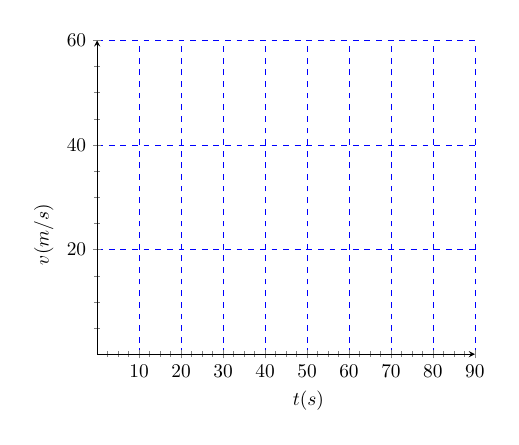
\begin{tikzpicture}[scale=0.7]
                \centering
                \begin{axis}
                    [axis lines = left,
                    axis x line=center,
                    axis y line=center,
                    mark=circle,
% xtick={-5,-4,...,5},
% ytick={-5,-4,...,5},
                    xlabel={$t(s)$},
                    ylabel={$v(m/s)$},
                    ylabel near ticks,
                    xlabel near ticks,
                    xlabel style={below right},
                    ylabel style={above left},
                    ymax=60,
                    ymin=0,
                    xmax=90,
                    xmin=0,
                    xtick={0,10,20,30,40,50,60,70,80,90},
                    ymajorgrids=true,
                    xmajorgrids=true,
                    minor tick num=3,
                    grid style={dashed, blue},
                    ]
                \end{axis}
        \end{tikzpicture}
        \caption{\textbf{Sistema de referencia}. Se representa la velocidad frente al tiempo.}
        \label{fig:reference_system}
    \end{figure}
\end{minipage}
\hfill
\begin{minipage}{0.45\textwidth}
    Decimos que un objeto está en movimiento cuando su posición cambia con respecto a un sistema de referencia a lo largo del tiempo.

    Si su posición no cambia, decimos que el objeto está en \textbf{reposo}.

    El movimiento es relativo, es decir, depende del punto de referencia, y por ello, para su estudio, es necesario establecer un sistema de referencia.

    En Física, el sistema de referencia será un sistema de coordenadas cartesianas \( x\ ,\ y \).
\end{minipage}

\vspace*{6pt}
\begin{definition}[Sistema de Referencia]
         Es un sistema que nos permite fijar la posición de un objeto y estudiar su evolución a lo largo del tiempo.
\end{definition}

\section{Magnitudes que describen el movimiento}

Para determinar el movimiento, necesitamos conocer las siguientes magnitudes:

\begin{enumerate}[label=\numberballmDarkTeal]
        \item \textbf{Posición}.
        Nos indica la ubicación exacta del objeto.
        La posición se suele representar mediante la letra \( x \), y su unidad en el SI es el metro (\( \unit{\metre} \)).

        \item \textbf{Desplazamiento}.
        Es la diferencia entre la posición final y la posición inicial del movimiento.
        El desplazamiento se representará como \( \Delta x \):

        \vspace*{20pt}
        \begin{centeredequation}
            \eqnmarkbox[blue]{displacement}{\Delta x}
            =
            \eqnmarkbox[red]{finalpos}{x_f}
            -
            \eqnmarkbox[mygreen]{initialpos}{x_i}
        \end{centeredequation}
        \vspace{25pt}
        \annotate[yshift=1em]{left}{displacement}{Desplazamiento}
        \annotate[yshift=1em]{}{finalpos}{Posición final}
        \annotate[yshift=-2em]{below,left}{initialpos}{Posición inicial}

        Matemáticamente, el símbolo \( \Delta \) indica la diferencia entre los valores final e inicial.

        Si este símbolo precede a una magnitud, significa el valor final menos el valor inicial de dicha magnitud.

        Para la posición, tendremos \( \Delta x = x_f - x_i \), para el tiempo \( \Delta t = t_f - t_i \), y para la velocidad \( \Delta v = v_f - v_i \).

        \item Su unidad también será el metro.

        \begin{remark}
            Aquí es importante señalar que el desplazamiento puede ser \textbf{negativo}.
            Esto ocurre cuando el objeto en movimiento se desplaza en sentido contrario.
        \end{remark}

        \item \textbf{Trayectoria}.
        Es el camino seguido durante el movimiento.

        \item \textbf{Distancia recorrida}.
        Es la longitud de la trayectoria.
        Su unidad también será el metro.
\end{enumerate}

El movimiento puede clasificarse según su trayectoria.
Así, tendremos:
\begin{enumerate}[label=\letraminuscula]
        \item \negsubro{Rectilíneo}.
        La trayectoria es una línea recta.
        En este tipo de movimiento, el desplazamiento coincide con la distancia recorrida.
        \item \negsubro{Circular}.
        La trayectoria es circular.
        \item \negsubro{Curvilíneo}.
        La trayectoria describe curvas.
\end{enumerate}

\begin{exercise}
    En tu cuaderno, identifica si la trayectoria de cada uno de los siguientes movimientos es recta (rectilínea) o curva (circular).
    \begin{enumerate}[label=\letraminuscula]
        \item una pelota que cae desde una altura
        \item una piedra atada a una cuerda y girada en círculos
        \item el movimiento de la manecilla de los segundos de un reloj
        \item un velocista que corre \qty{100}{\metre} en una pista recta
    \end{enumerate}
%    Página 135, Ejericio 11
    \begin{solu}
        \textbf{\textcolor{purple}{Ejercicio:}} En tu cuaderno, identifica si la trayectoria de cada uno de los siguientes movimientos es recta (rectilínea) o curva (circular).
        \begin{enumerate}[label=\letraminuscula]
            \item una pelota que cae desde una altura
            \item una piedra atada a una cuerda y girada en círculos
            \item el movimiento de la manecilla de los segundos de un reloj
            \item un velocista que corre \qty{100}{\metre} en una pista recta
        \end{enumerate}

        \vspace{0.3cm}

        \begin{enumerate}[label=\letraminuscula]
            \item \textcolor{blue}{Rectilínea (línea recta)} - Una pelota que cae se mueve verticalmente hacia abajo en una trayectoria recta debido a la gravedad.
            \item \textcolor{blue}{Circular} - Una piedra atada a una cuerda y girada traza una trayectoria circular alrededor del punto central.
            \item \textcolor{blue}{Circular} - La manecilla de los segundos de un reloj se mueve en una trayectoria circular alrededor de la esfera del reloj.
            \item \textcolor{blue}{Rectilínea (línea recta)} - Un velocista que corre 100 m en una pista recta sigue una trayectoria lineal.
        \end{enumerate}
    \end{solu}
\end{exercise}

\begin{exercise}
    Imagina que das una vuelta completa a una rotonda circular y regresas a tu posición de partida. ¿Cuál es tu desplazamiento total?
    \begin{solu}
        \textbf{\textcolor{purple}{Ejercicio:}} Imagina que das una vuelta completa a una rotonda circular y regresas a tu posición de partida. ¿Cuál es tu desplazamiento total?

        \vspace{0.3cm}

        \textcolor{red}{Concepto clave:} El desplazamiento es una magnitud vectorial que mide el cambio de posición desde el punto inicial hasta el punto final.

        \textcolor{blue}{Datos:}
        \begin{itemize}
            \item Posición inicial = Posición final (regresas al lugar donde empezaste)
        \end{itemize}

        \textcolor{blue}{Análisis:}

        El desplazamiento se define como:
        \[
            \vec{\Delta x} = \vec{x}_{\text{final}} - \vec{x}_{\text{inicial}}
        \]

        Dado que regresas al punto de partida:
        \[
            \vec{x}_{\text{final}} = \vec{x}_{\text{inicial}}
        \]

        Por lo tanto:
        \[
            \vec{\Delta x} = \vec{x}_{\text{inicial}} - \vec{x}_{\text{inicial}} = \vec{0}
        \]

        \textcolor{red}{Respuesta:} El desplazamiento es \textbf{cero} (\qty{0}{\m}), aunque hayas recorrido una cierta distancia alrededor de la rotonda. Esto demuestra la diferencia entre distancia (longitud total del camino recorrido) y desplazamiento (cambio de posición en línea recta).
    \end{solu}
\end{exercise}

\begin{exercise}
    Si das toda la vuelta a una rotonda y regresas al punto de partida, ¿cuál es tu desplazamiento?
    \begin{solu}
        El desplazamiento es la distancia en línea recta entre el inicio y el final.
        \begin{itemize}
            \item \textbf{Posición inicial ($x_i$):} Punto A.
            \item \textbf{Posición final ($x_f$):} Punto A.
            \item \textbf{Cálculo:} $\Delta x = x_f - x_i = A - A = \mathbf{0}$.
        \end{itemize}
        El desplazamiento es \textcolor{red}{\qty{0}{\m}}. Observa que la \textit{distancia recorrida} es el perímetro de la rotonda, pero el desplazamiento es cero.
    \end{solu}
\end{exercise}


\section{Velocidad}

La velocidad nos da una medida de la rapidez con la que se mueve un objeto.
Tenemos dos tipos de velocidad:

\begin{enumerate}[label=\numberballmDarkTeal]
        \item \textbf{Velocidad instantánea}.
        Es la velocidad que tiene un objeto en un instante dado.
        Podemos verla en el velocímetro de un coche, ya que la velocidad cambia constantemente.

        \item \textbf{Velocidad media}.
        Esta es la medida de velocidad que utilizaremos en este curso y la representaremos con la letra \( v \).
        \begin{centeredequation}
            v = \dfrac{\text{Desplazamiento}}{\text{Tiempo transcurrido}} = \dfrac{\Delta x}{\Delta t}
        \end{centeredequation}

        \item Si expresamos esto en términos de la posición inicial y final, tenemos:
        \begin{centeredequation}
            v = \dfrac{x_f - x_i}{t_f - t_i}
        \end{centeredequation}
        \begin{itemize}
            \item \( x_i \) es la posición inicial.
            \item \( t_i \) es el tiempo medido en la posición inicial.
            \item \( x_f \) es la posición final.
            \item \( t_f \) es el tiempo medido en la posición final.
        \end{itemize}
\end{enumerate}

Las unidades del SI para la velocidad son: \unit{\mps}


\section{Aceleración}

La aceleración nos indica cómo cambia la velocidad con el tiempo.
Al igual que la velocidad, tenemos dos tipos de aceleración:

\begin{enumerate}[label=\numberballmDarkTeal]
        \item \textbf{Aceleración instantánea}.
        Es la aceleración en un instante dado.

        \item \textbf{Aceleración media}.
        Es la aceleración a lo largo de un periodo de tiempo.
        Esta es la que utilizaremos en este tema.
        La fórmula se expresa como:
        \begin{centeredequation}
            a = \dfrac{\text{Cambio de velocidad}}{\text{Tiempo transcurrido}} = \dfrac{\Delta v}{\Delta t}
        \end{centeredequation}

        \item Si expresamos esto en términos de la velocidad inicial y final, tenemos:
        \begin{centeredequation}
            a = \dfrac{v_f - v_i}{t_f - t_i}
        \end{centeredequation}
        \begin{itemize}
            \item \( v_i \) es la velocidad inicial.
            \item \( t_i \) es el tiempo medido en la velocidad inicial.
            \item \( v_f \) es la velocidad final.
            \item \( t_f \) es el tiempo medido en la velocidad final.
        \end{itemize}
\end{enumerate}

Las unidades del SI para la aceleración son: \unit{\mpss}


\section{Movimiento Rectilíneo}

Los movimientos rectilíneos son aquellos que tienen una \textbf{trayectoria en línea recta}.
Estos movimientos son muy interesantes porque, en estos casos, \textbf{el desplazamiento coincide con la distancia recorrida}.

Las ecuaciones descritas anteriormente para la velocidad y la aceleración pueden escribirse como:
\begin{centeredequation}
    v = \dfrac{\Delta x}{\Delta t} \longrightarrow v = \dfrac{x_f - x_i}{t_f - t_i}
\end{centeredequation}
\begin{centeredequation}
    a = \dfrac{\Delta v}{\Delta t} \longrightarrow a = \dfrac{v_f - v_i}{t_f - t_i}
\end{centeredequation}
A veces estas expresiones pueden simplificarse porque:
\begin{itemize}
    \item Generalmente, tomamos \( t_i = 0 \), por lo que este término puede eliminarse.
    Podemos elegir el instante inicial.
    \item Como solo queda un término de tiempo, \( t_f \) puede simplificarse simplemente como \( t \).
    \item Lo mismo se aplica a \( x_i \), aunque es menos habitual.
    Si fijamos la posición inicial \( x_i = 0 \), puede eliminarse, y la posición final \( x_f \) puede llamarse simplemente \( x \).
    \item La misma simplificación puede aplicarse también a \( v_i \).
\end{itemize}
Tras estas simplificaciones, las ecuaciones quedan:
\begin{centeredequation}
    v = \dfrac{x}{t}
\end{centeredequation}
\begin{centeredequation}
    a = \dfrac{v}{t}
\end{centeredequation}
\begin{remark}
    Aunque podamos simplificar las expresiones, es importante leer con atención el enunciado del problema para comprobar si la simplificación está permitida.
\end{remark}

\subsection{Movimiento Rectilíneo Uniforme (MRU)}

Este es un caso particular de movimiento rectilíneo con las siguientes condiciones:
\begin{itemize}
    \item Su trayectoria es una línea recta.
    \item Su velocidad no cambia durante el movimiento. Por lo tanto:
    \begin{itemize}
        \item \( v_f = v_i \)
        \item \( \Delta v = 0 \)
    \end{itemize}
    \item Dado que la velocidad no cambia, la aceleración es cero, es decir, \( a = \qty{0}{\mpss} \)

    \begin{theorem}[]
        La velocidad viene dada por: $v = \dfrac{x_f - x_i}{t_f-t_i}$. Aplicando las simplificaciones anteriores: \(  v = \dfrac{x}{t}  \)

%        To find the final position:
%        \begin{centeredequation}
%            x_f = x_i + v\cdot (t_f-t_i)
%        \end{centeredequation}
%        If \( t_i = 0 \):
%        \begin{centeredequation}
%            x_f = x_i + v\cdot t
%        \end{centeredequation}
%        If also \( x_i = 0 \):
%        \begin{centeredequation}
%            x = v\cdot t
%        \end{centeredequation}
%        To find \( t_f \):
%        \begin{centeredequation}
%            t_f = t_i + \dfrac{x_f-x_i}{v}
%        \end{centeredequation}
%        If \( t_i = 0 \):
%        \begin{centeredequation}
%            t = \dfrac{x_f-x_i}{v}
%        \end{centeredequation}
%        If \( x_i = 0 \):
%        \begin{centeredequation}
%            t = \dfrac{x}{v}
%        \end{centeredequation}
    \end{theorem}
\end{itemize}


%    Página 135, Ejericio 12

\begin{exercise}
    El Sol se encuentra a una distancia media de \qty{1.5e8}{\kilo\m} de la Tierra, y la velocidad de la luz en el vacío es \qty{3e8}{\mps}. Suponiendo que la luz viaja a velocidad constante (movimiento rectilíneo uniforme), calcula cuánto tiempo tarda la luz del Sol en llegar a la Tierra.

    \begin{solu}
        \textbf{\textcolor{purple}{Ejercicio:}} El Sol se encuentra a una distancia media de \qty{1.5e8}{\kilo\m} de la Tierra, y la velocidad de la luz en el vacío es \qty{3e8}{\mps}. Suponiendo que la luz viaja a velocidad constante (movimiento rectilíneo uniforme), calcula cuánto tiempo tarda la luz del Sol en llegar a la Tierra.

        \vspace{0.3cm}

        \textcolor{blue}{Datos:}
        \begin{itemize}
            \item Distancia del Sol a la Tierra: $d = \qty{1.5e8}{\kilo\m}$
            \item Velocidad de la luz: $v = \qty{3e8}{\mps}$
            \item Tipo de movimiento: Movimiento rectilíneo uniforme (velocidad constante)
        \end{itemize}

        \textcolor{blue}{Paso 1: Convertir todas las unidades al SI (metros y segundos)}
        \[
            d = 1.5 \times 10^8 \text{ km} \times \frac{1000 \text{ m}}{1 \text{ km}} = \textcolor{red}{1.5 \times 10^{11} \text{ m}}
        \]

        \textcolor{blue}{Paso 2: Aplicar la fórmula del movimiento uniforme}

        Para el movimiento rectilíneo uniforme, la relación entre distancia, velocidad y tiempo es:
        \[
            \boxed{d = v \cdot t}
        \]

        \textcolor{blue}{Paso 3: Despejar el tiempo}

        Reordenando la ecuación:
        \[
            t = \frac{d}{v}
        \]

        \textcolor{blue}{Paso 4: Sustituir valores y calcular}
        \[
            t = \frac{1.5 \times 10^{11} \text{ m}}{3 \times 10^8 \text{ m/s}} = \frac{1.5}{3} \times 10^{11-8} \text{ s} = 0.5 \times 10^3 \text{ s} = \textcolor{red}{500 \text{ s}}
        \]

        \textcolor{blue}{Paso 5: Convertir a minutos (opcional)}
        \[
            t = 500 \text{ s} \times \frac{1 \text{ min}}{60 \text{ s}} = \textcolor{red}{8.33 \text{ min}} \approx 8 \text{ min } 20 \text{ s}
        \]

        \textcolor{red}{Respuesta:} La luz tarda aproximadamente \textbf{500 segundos} (u \textbf{8 minutos y 20 segundos}) en viajar desde el Sol hasta la Tierra.
    \end{solu}
\end{exercise}


\begin{exercise}
    Durante una clase de Educación Física, estás cronometrando cuánto tardan los estudiantes en correr \qty{100}{\m}.
    \begin{enumerate}[label=\letraminuscula]
        \item Si una de tus compañeras completa los \qty{100}{\m} en \qty{15}{\s}, ¿cuál es su velocidad media?
        \item De media, ¿cuántos metros recorre cada segundo?
    \end{enumerate}
    \begin{solu}
        \textbf{\textcolor{purple}{Ejercicio:}} Durante una clase de Educación Física, estás cronometrando cuánto tardan los estudiantes en correr \qty{100}{\m}.
        \begin{enumerate}[label=\letraminuscula]
            \item Si una de tus compañeras completa los \qty{100}{\m} en \qty{15}{\s}, ¿cuál es su velocidad media?
            \item De media, ¿cuántos metros recorre cada segundo?
        \end{enumerate}

        \vspace{0.3cm}

        \textcolor{blue}{Datos:}
        \begin{itemize}
            \item Distancia: $d = \qty{100}{\m}$
            \item Tiempo: $t = \qty{15}{\s}$
        \end{itemize}

        \textbf{\textcolor{blue}{Apartado a) Calcular la velocidad media}}

        \textcolor{blue}{Paso 1: Aplicar la fórmula de la velocidad media}

        La velocidad media se define como:
        \[
            \boxed{v_{\text{media}} = \frac{d}{t}}
        \]

        \textcolor{blue}{Paso 2: Sustituir valores y calcular}
        \[
            v_{\text{media}} = \frac{100 \text{ m}}{15 \text{ s}} = \textcolor{red}{6.67 \text{ m/s}}
        \]

        \textcolor{red}{Respuesta a):} Su velocidad media es \textbf{\qty{6.67}{\mps}}.

        \vspace{0.5cm}

        \textbf{\textcolor{blue}{Apartado b) Metros por segundo}}

        \textcolor{blue}{Análisis:} La pregunta plantea «cuántos metros recorre por segundo», que es exactamente la definición de la rapidez en m/s.

        \textcolor{red}{Respuesta b):} Recorre una media de \textbf{6,67 metros por segundo}. Este es el mismo valor que la velocidad calculada en el apartado a), ya que la velocidad se mide en metros por segundo (m/s).
    \end{solu}
\end{exercise}



\begin{exercise}
    Durante un viaje familiar en coche, tu coche circula por una autovía recta a una velocidad media de \qty{90}{\kmph} durante \qty{15}{min}.
    \begin{enumerate}[label=\letraminuscula]
        \item Calcula la distancia recorrida en metros durante este periodo de tiempo.
        \item ¿Puedes estar seguro de que la velocidad del coche fue exactamente \qty{90}{\kmph} en todo momento durante el trayecto?
    \end{enumerate}
    \begin{solu}
        \textbf{\textcolor{purple}{Ejercicio:}} Durante un viaje familiar en coche, tu coche circula por una autovía recta a una velocidad media de \qty{90}{\kmph} durante \qty{15}{min}.
        \begin{enumerate}[label=\letraminuscula]
            \item Calcula la distancia recorrida en metros durante este periodo de tiempo.
            \item ¿Puedes estar seguro de que la velocidad del coche fue exactamente \qty{90}{\kmph} en todo momento durante el trayecto?
        \end{enumerate}

        \vspace{0.3cm}

        \textcolor{blue}{Datos:}
        \begin{itemize}
            \item Velocidad media: $v_{\text{media}} = \qty{90}{\kmph}$
            \item Tiempo: $t = \qty{15}{min}$
        \end{itemize}

        \textbf{\textcolor{blue}{Apartado a) Calcular la distancia en metros}}

        \textcolor{blue}{Paso 1: Convertir las unidades al SI}

        Convertir la velocidad de km/h a m/s:
        \[
            v = 90 \frac{\text{km}}{\text{h}} \times \frac{1000 \text{ m}}{1 \text{ km}} \times \frac{1 \text{ h}}{3600 \text{ s}} = 90 \times \frac{1000}{3600} = \textcolor{red}{25 \text{ m/s}}
        \]

        Convertir el tiempo de minutos a segundos:
        \[
            t = 15 \text{ min} \times \frac{60 \text{ s}}{1 \text{ min}} = \textcolor{red}{900 \text{ s}}
        \]

        \textcolor{blue}{Paso 2: Aplicar la fórmula de la distancia}
        \[
            \boxed{d = v \cdot t}
        \]

        \textcolor{blue}{Paso 3: Calcular la distancia}
        \[
            d = 25 \text{ m/s} \times 900 \text{ s} = \textcolor{red}{22\,500 \text{ m}}
        \]

        \textcolor{red}{Respuesta a):} El coche recorrió \textbf{\qty{22500}{\m}} (o 22,5 km) durante esos 15 minutos.

        \vspace{0.5cm}

        \textbf{\textcolor{blue}{Apartado b) ¿Fue la velocidad constante?}}

        \textcolor{blue}{Análisis:} El enunciado indica que 90 km/h es la velocidad \textit{media}, no la velocidad instantánea.

        \textcolor{red}{Respuesta b):} \textbf{No}, no podemos estar seguros de que la velocidad fuera exactamente 90 km/h en todo momento. El valor de 90 km/h es la \textit{velocidad media} durante el intervalo de 15 minutos. Durante el trayecto, el coche pudo haber circulado más rápido o más despacio en distintos momentos (por ejemplo, acelerando para adelantar, reduciendo la velocidad en las curvas, etc.), siempre que la media a lo largo de todo el periodo de tiempo sea igual a 90 km/h.
    \end{solu}
\end{exercise}


\begin{exercise}
    Un coche que circula por una autovía recta lleva viajando durante \qty{30}{min} a una velocidad media de \qty{100}{\kmph}. ¿Qué distancia, en metros, ha recorrido el coche durante este tiempo?
    \begin{solu}
        \textbf{\textcolor{purple}{Ejercicio:}} Un coche que circula por una autovía recta lleva viajando durante \qty{30}{min} a una velocidad media de \qty{100}{\kmph}. ¿Qué distancia, en metros, ha recorrido el coche durante este tiempo?

        \vspace{0.3cm}

        \textcolor{blue}{Datos:}
        \begin{itemize}
            \item Velocidad media: $v_{\text{media}} = \qty{100}{\kmph}$
            \item Tiempo: $t = \qty{30}{min}$
        \end{itemize}

        \textcolor{blue}{Paso 1: Convertir las unidades al SI}

        Convertir la velocidad de km/h a m/s:
        \[
            v = 100 \frac{\text{km}}{\text{h}} \times \frac{1000 \text{ m}}{1 \text{ km}} \times \frac{1 \text{ h}}{3600 \text{ s}} = 100 \times \frac{1000}{3600} = \textcolor{red}{27.78 \text{ m/s}}
        \]

        Convertir el tiempo de minutos a segundos:
        \[
            t = 30 \text{ min} \times \frac{60 \text{ s}}{1 \text{ min}} = \textcolor{red}{1800 \text{ s}}
        \]

        \textcolor{blue}{Paso 2: Aplicar la fórmula de la distancia para el movimiento uniforme}
        \[
            \boxed{d = v \cdot t}
        \]

        \textcolor{blue}{Paso 3: Sustituir valores y calcular}
        \[
            d = 27.78 \text{ m/s} \times 1800 \text{ s} = \textcolor{red}{50\,000 \text{ m}}
        \]

        \textcolor{red}{Respuesta:} El coche ha recorrido \textbf{\qty{50000}{\m}} (o 50 km) durante los 30 minutos.
    \end{solu}
\end{exercise}


\begin{exercise}
    Un coche se mueve por una carretera recta, y su velocidad cambia de la siguiente manera: Tras \qty{1}{\s}, su velocidad es \qty{2}{\mps}. Tras \qty{2}{\s} desde el inicio, su velocidad es \qty{4}{\mps}. Tras \qty{3}{\s}, su velocidad es \qty{6}{\mps}.

    \begin{enumerate}[label=\letraminuscula]
        \item ¿En cuánto cambia la velocidad del coche durante cada segundo?
        \item ¿Cuál es la aceleración de este vehículo?
    \end{enumerate}
    \begin{solu}
        \textbf{\textcolor{purple}{Ejercicio:}} Un coche se mueve por una carretera recta, y su velocidad cambia de la siguiente manera: Tras \qty{1}{\s}, su velocidad es \qty{2}{\mps}. Tras \qty{2}{\s} desde el inicio, su velocidad es \qty{4}{\mps}. Tras \qty{3}{\s}, su velocidad es \qty{6}{\mps}.
        \begin{enumerate}[label=\letraminuscula]
            \item ¿En cuánto cambia la velocidad del coche durante cada segundo?
            \item ¿Cuál es la aceleración de este vehículo?
        \end{enumerate}

        \vspace{0.3cm}

        \textcolor{blue}{Datos:}
        \begin{itemize}
            \item En $t_1 = 1$ s: $v_1 = \qty{2}{\mps}$
            \item En $t_2 = 2$ s: $v_2 = \qty{4}{\mps}$
            \item En $t_3 = 3$ s: $v_3 = \qty{6}{\mps}$
        \end{itemize}

        \textbf{\textcolor{blue}{Apartado a) Cambio de velocidad por segundo}}

        \textcolor{blue}{Paso 1: Calcular los cambios de velocidad}

        Cambio durante el primer segundo (de $t=0$ a $t=1$ s):
        \[
            \Delta v_1 = v_1 - v_0 = 2 - 0 = \textcolor{red}{2 \text{ m/s}}
        \]

        Cambio durante el segundo segundo (de $t=1$ a $t=2$ s):
        \[
            \Delta v_2 = v_2 - v_1 = 4 - 2 = \textcolor{red}{2 \text{ m/s}}
        \]

        Cambio durante el tercer segundo (de $t=2$ a $t=3$ s):
        \[
            \Delta v_3 = v_3 - v_2 = 6 - 4 = \textcolor{red}{2 \text{ m/s}}
        \]

        \textcolor{red}{Respuesta a):} La velocidad del coche aumenta en \textbf{\qty{2}{\mps}} durante cada segundo.

        \vspace{0.5cm}

        \textbf{\textcolor{blue}{Apartado b) Calcular la aceleración}}

        \textcolor{blue}{Paso 2: Aplicar la fórmula de la aceleración}

        La aceleración se define como la tasa de cambio de la velocidad:
        \[
            \boxed{a = \frac{\Delta v}{\Delta t}}
        \]

        Dado que la velocidad cambia en 2 m/s cada 1 segundo:
        \[
            a = \frac{2 \text{ m/s}}{1 \text{ s}} = \textcolor{red}{2 \text{ m/s}^2}
        \]

        \textcolor{blue}{Cálculo alternativo usando dos puntos cualesquiera:}
        \[
            a = \frac{v_3 - v_1}{t_3 - t_1} = \frac{6 - 2}{3 - 1} = \frac{4}{2} = \textcolor{red}{2 \text{ m/s}^2}
        \]

        \textcolor{red}{Respuesta b):} La aceleración del vehículo es \textbf{\qty{2}{\metre\per\second\squared}}.

        \textcolor{blue}{Nota:} Dado que la aceleración es constante y positiva, se trata de un movimiento uniformemente acelerado.
    \end{solu}
\end{exercise}

\begin{exercise}
    Un ciclista sale de Almansa por el carril bici a una velocidad de \qty{8}{\mps}.
    Si tarda \qty{100}{\min} en llegar a su destino:
    \begin{enumerate}[label=\letraminuscula]
    \item ¿Qué distancia ha recorrido?
    \item Sabiendo que Bonete está a \qty{32}{\km}, ¿cuánto tardaría en llegar?
    \end{enumerate}
\end{exercise}

\subsubsection{Gráficas del Movimiento Rectilíneo Uniforme (MRU)}
En física, es muy habitual elaborar gráficas y, a partir de ellas, identificar el tipo de movimiento. Para el MRU, tendremos los siguientes casos.
\begin{figure}[H]
    \centering
    % First subfigure
    \begin{subfigure}[b]{0.45\textwidth}
        \centering
        \begin{tikzpicture}[scale=0.85]
            \begin{axis}
                [
                ylabel={$x$ (\unit{\m})},
                xlabel={$t$ (\unit{\s})},
                axis lines=middle,
                enlargelimits=true,
                xmin=0, xmax=10,
                ymin=0, ymax=10,
                domain=0:8,
                samples=100,
                legend pos=outer north east,
                legend style={draw=none},
                xticklabels={},
                yticklabels={}
                ]
                \addplot[line width=1.5pt, red] {3 + 0.5*x};
            \end{axis}
        \end{tikzpicture}
        \caption{Posición frente a Tiempo. Moviéndose en sentido positivo.}
    \end{subfigure}
    \hfill
    % Second subfigure
    \begin{subfigure}[b]{0.45\textwidth}
        \centering
        \begin{tikzpicture}[scale=0.85]
            \begin{axis}
                [
                ylabel={$x$ (\unit{\m})},
                xlabel={$t$ (\unit{\s})},
                axis lines=middle,
                enlargelimits=true,
                xmin=0, xmax=10,
                ymin=0, ymax=10,
                domain=0:8,
                samples=100,
                legend pos=outer north east,
                legend style={draw=none},
                xticklabels={},
                yticklabels={}
                ]
                \addplot[line width=1.5pt, red] {8 - 0.5*x};
            \end{axis}
        \end{tikzpicture}
        \caption{Posición frente a Tiempo. Moviéndose en sentido contrario.}
    \end{subfigure}
\end{figure}

\begin{figure}[H]
    \centering
    % First subfigure
    \begin{subfigure}[b]{0.45\textwidth}
        \centering
        \begin{tikzpicture}[scale=0.85]
            \begin{axis}
                [
                ylabel={$v$ (\unit{\mps})},
                xlabel={$t$ (\unit{\s})},
                axis lines=middle,
                enlargelimits=true,
                xmin=0, xmax=10,
                ymin=0, ymax=10,
                domain=0:8,
                samples=100,
                legend pos=outer north east,
                legend style={draw=none},
                xticklabels={},
                yticklabels={}
                ]
                \addplot[line width=1.5pt, red] {5};
            \end{axis}
        \end{tikzpicture}
        \caption{Velocidad frente a Tiempo. Moviéndose en sentido positivo.}
    \end{subfigure}
    \hfill
    % Second subfigure
    \begin{subfigure}[b]{0.45\textwidth}
        \centering
        \begin{tikzpicture}[scale=0.85]
            \begin{axis}
                [
                ylabel={$a$ (\unit{\mpss})},
                xlabel={$t$ (\unit{\s})},
                axis lines=middle,
                enlargelimits=true,
                xmin=0, xmax=10,
                ymin=-1, ymax=10,
                domain=0:8,
                samples=100,
                legend style={draw=none},
                xticklabels={},
                yticklabels={}
                ]
                \addplot[line width=2pt, red] {0};
            \end{axis}
        \end{tikzpicture}
        \caption{Aceleración frente a Tiempo.}
    \end{subfigure}
\end{figure}
%\begin{remark}
%    If the motion is in the opposite direction, the velocity vs time graph would look like:
%    \begin{figure}[H]
%        \centering
%        \begin{tikzpicture}[scale=0.85]
%            \begin{axis}
%                [
%                ylabel={$v$ (\unit{\mps})},
%                xlabel={$t$ (\unit{\s})},
%                axis lines=middle,
%                enlargelimits=true,
%                xmin=-10, xmax=2,
%                ymin=0, ymax=10,
%                domain=-10:2,
%                samples=100,
%                legend pos=outer north east,
%                legend style={draw=none},
%                xticklabels={},
%                yticklabels={}
%                ]
%                \addplot[line width=1.5pt, red] {-5};
%            \end{axis}
%        \end{tikzpicture}
%        \caption{Velocity vs Time. Moving in the opposite direction.}
%    \end{figure}
%\end{remark}


\subsection{Movimiento Rectilíneo Uniformemente Acelerado (MRUA)}

Este es otro caso particular de movimiento rectilíneo que cumple las siguientes condiciones:
\begin{itemize}
    \item La trayectoria también es una línea recta.
    \item Ahora, la velocidad cambia durante el movimiento.
    \begin{itemize}
        \item \( v_f \neq v_i \)
        \item \( \Delta v \neq  0 \)
    \end{itemize}
    \item Dado que la velocidad cambia, la aceleración ahora es distinta de cero (\( a \neq 0 \)) pero constante, lo que significa que la aceleración no varía.
\end{itemize}

Las ecuaciones de este movimiento son las siguientes:
\begin{itemize}
    \item Para la aceleración tenemos:
    \begin{centeredequation}
        a = \dfrac{v_f - v_i}{t_f - t_i} \label{eq:aceleracion_general}
    \end{centeredequation}
    Si aplicamos las simplificaciones \( v_i = 0 \) y \( t_i = 0 \), obtenemos:
    \begin{centeredequation}
        a = \dfrac{v}{t}
    \end{centeredequation}
    \item La ecuación de la posición es:
    \begin{centeredequation}
        x_f = x_i + v_i\cdot (t_f - t_i) + \frac{1}{2} \cdot a \cdot (t_f - t_i)^2 \label{eq:posición_general}
    \end{centeredequation}
    Si simplificamos suponiendo que el instante inicial es \( t_i = 0 \), la ecuación queda:
    \begin{centeredequation}
        x_f = x_i + v_i \cdot t + \frac{1}{2} \cdot a \cdot t^2
    \end{centeredequation}
    Si además suponemos que la posición inicial es cero (\( x_i = 0 \)), esta expresión se simplifica aún más:
    \begin{centeredequation}
        x = v_i \cdot t + \frac{1}{2} \cdot a \cdot t^2
    \end{centeredequation}
    Como podemos observar, en esta ecuación \( v_f \) nunca aparece, lo que significa que la posición final no depende de la velocidad final, pero sí depende de la velocidad inicial, ya que esta aparece en la fórmula.
    \item Debido a la complejidad de despejar el tiempo en este tipo de movimiento, la expresión no se estudiará en este curso.
\end{itemize}


\begin{exercise}
    Has ido a esquiar con tus compañeros de clase y decides bajar por una pista. Partiendo del reposo, aceleras hasta \qty{10}{\mps} en \qty{5}{\s}. ¿Cuál fue tu aceleración media?
    \begin{solu}
        \textbf{\textcolor{purple}{Ejercicio:}} Has ido a esquiar con tus compañeros de clase y decides bajar por una pista. Partiendo del reposo, aceleras hasta \qty{10}{\mps} en \qty{5}{\s}. ¿Cuál fue tu aceleración media?

        \vspace{0.3cm}

        \textcolor{blue}{Datos:}
        \begin{itemize}
            \item Velocidad inicial: $v_0 = \qty{0}{\mps}$ (partiendo del reposo)
            \item Velocidad final: $v_f = \qty{10}{\mps}$
            \item Intervalo de tiempo: $\Delta t = \qty{5}{\s}$
        \end{itemize}

        \textcolor{blue}{Paso 1: Aplicar la fórmula de la aceleración}

        La aceleración se define como el cambio de velocidad dividido por el intervalo de tiempo:
        \[
            \boxed{a = \frac{\Delta v}{\Delta t} = \frac{v_f - v_0}{\Delta t}}
        \]

        \textcolor{blue}{Paso 2: Calcular el cambio de velocidad}
        \[
            \Delta v = v_f - v_0 = 10 - 0 = \textcolor{red}{10 \text{ m/s}}
        \]

        \textcolor{blue}{Paso 3: Calcular la aceleración}
        \[
            a = \frac{10 \text{ m/s}}{5 \text{ s}} = \textcolor{red}{2 \text{ m/s}^2}
        \]

        \textcolor{red}{Respuesta:} Tu aceleración media al bajar por la pista fue \textbf{\qty{2}{\metre\per\second\squared}}.

        \textcolor{blue}{Interpretación física:} Esto significa que tu velocidad aumentó 2 m/s cada segundo durante el descenso.
    \end{solu}
\end{exercise}


\begin{exercise}
    Un vehículo acelera desde el reposo hasta \qty{100}{\kmph} en \qty{8}{\s}. Calcula su aceleración media, dando tu respuesta en \unit{\mpss}.
    \begin{solu}
        \textbf{\textcolor{purple}{Ejercicio:}} Un vehículo acelera desde el reposo hasta \qty{100}{\kmph} en \qty{8}{\s}. Calcula su aceleración media, dando tu respuesta en \unit{\mpss}.

        \vspace{0.3cm}

        \textcolor{blue}{Datos:}
        \begin{itemize}
            \item Velocidad inicial: $v_0 = \qty{0}{\kmph}$ (partiendo del reposo)
            \item Velocidad final: $v_f = \qty{100}{\kmph}$
            \item Intervalo de tiempo: $\Delta t = \qty{8}{\s}$
        \end{itemize}

        \textcolor{blue}{Paso 1: Convertir la velocidad a m/s}

        Velocidad inicial (ya es cero en cualquier unidad):
        \[
            v_0 = 0 \text{ m/s}
        \]

        Velocidad final:
        \[
            v_f = 100 \frac{\text{km}}{\text{h}} \times \frac{1000 \text{ m}}{1 \text{ km}} \times \frac{1 \text{ h}}{3600 \text{ s}} = 100 \times \frac{1000}{3600} = \textcolor{red}{27.78 \text{ m/s}}
        \]

        \textcolor{blue}{Paso 2: Aplicar la fórmula de la aceleración}
        \[
            \boxed{a = \frac{\Delta v}{\Delta t} = \frac{v_f - v_0}{\Delta t}}
        \]

        \textcolor{blue}{Paso 3: Calcular el cambio de velocidad}
        \[
            \Delta v = v_f - v_0 = 27.78 - 0 = \textcolor{red}{27.78 \text{ m/s}}
        \]

        \textcolor{blue}{Paso 4: Calcular la aceleración}
        \[
            a = \frac{27.78 \text{ m/s}}{8 \text{ s}} = \textcolor{red}{3.47 \text{ m/s}^2}
        \]

        \textcolor{red}{Respuesta:} La aceleración media del vehículo es \textbf{\qty{3.47}{\metre\per\second\squared}}.

        \textcolor{blue}{Interpretación física:} La velocidad del vehículo aumenta aproximadamente 3,47 m/s cada segundo durante el periodo de aceleración.
    \end{solu}
\end{exercise}


\begin{exercise}
    Un coche que circula a \qty{30}{\mps} frena durante \qty{5}{\s}, reduciendo su velocidad a \qty{25}{\mps}. Determina su aceleración media durante el frenado.
    \begin{solu}
        \textbf{\textcolor{purple}{Ejercicio:}} Un coche que circula a \qty{30}{\mps} frena durante \qty{5}{\s}, reduciendo su velocidad a \qty{25}{\mps}. Determina su aceleración media durante el frenado.

        \vspace{0.3cm}

        \textcolor{blue}{Datos:}
        \begin{itemize}
            \item Velocidad inicial: $v_0 = \qty{30}{\mps}$
            \item Velocidad final: $v_f = \qty{25}{\mps}$
            \item Intervalo de tiempo: $\Delta t = \qty{5}{\s}$
        \end{itemize}

        \textcolor{blue}{Paso 1: Aplicar la fórmula de la aceleración}
        \[
            \boxed{a = \frac{\Delta v}{\Delta t} = \frac{v_f - v_0}{\Delta t}}
        \]

        \textcolor{blue}{Paso 2: Calcular el cambio de velocidad}
        \[
            \Delta v = v_f - v_0 = 25 - 30 = \textcolor{red}{-5 \text{ m/s}}
        \]

        \textcolor{blue}{Nota:} El cambio de velocidad es negativo porque el coche está frenando.

        \textcolor{blue}{Paso 3: Calcular la aceleración}
        \[
            a = \frac{-5 \text{ m/s}}{5 \text{ s}} = \textcolor{red}{-1 \text{ m/s}^2}
        \]

        \textcolor{red}{Respuesta:} La aceleración media durante el frenado es \textbf{\qty{-1}{\metre\per\second\squared}}.

        \textcolor{blue}{Interpretación física:} El signo negativo indica que se trata de una deceleración (el coche está frenando). El valor absoluto de la aceleración es 1 m/s², lo que significa que la velocidad del coche disminuye 1 m/s cada segundo durante el frenado.
    \end{solu}
\end{exercise}


\begin{exercise}
    Para despegar, un avión Airbus necesita alcanzar una velocidad de \qty{300}{\kmph} en un tiempo de \qty{23.8}{\s}. Calcula:
    \begin{enumerate}[label=\letraminuscula]
    \item ¿Cuál es su aceleración?
    \item ¿Cuál es la longitud mínima de pista necesaria?
    \end{enumerate}
    \begin{solu}
        \textbf{\textcolor{purple}{Ejercicio:}} Para despegar, un avión Airbus necesita alcanzar una velocidad de \qty{300}{\kmph} en un tiempo de \qty{23.8}{\s}. Calcula:
        \begin{enumerate}[label=\letraminuscula]
            \item ¿Cuál es su aceleración?
            \item ¿Cuál es la longitud mínima de pista necesaria?
        \end{enumerate}

        \vspace{0.3cm}

        \textcolor{blue}{Datos:}
        \begin{itemize}
            \item Velocidad inicial: $v_0 = \qty{0}{\kmph}$ (parte del reposo)
            \item Velocidad final: $v_f = \qty{300}{\kmph}$
            \item Tiempo: $t = \qty{23.8}{\s}$
        \end{itemize}

        \textbf{\textcolor{blue}{Apartado a) Calcular la aceleración}}

        \textcolor{blue}{Paso 1: Convertir la velocidad a m/s}
        \[
            v_0 = 0 \text{ m/s}
        \]
        \[
            v_f = 300 \frac{\text{km}}{\text{h}} \times \frac{1000 \text{ m}}{1 \text{ km}} \times \frac{1 \text{ h}}{3600 \text{ s}} = 300 \times \frac{1000}{3600} = \textcolor{red}{83.33 \text{ m/s}}
        \]

        \textcolor{blue}{Paso 2: Aplicar la fórmula de la aceleración}
        \[
            \boxed{a = \frac{v_f - v_0}{t}}
        \]

        \textcolor{blue}{Paso 3: Calcular la aceleración}
        \[
            a = \frac{83.33 - 0}{23.8} = \frac{83.33}{23.8} = \textcolor{red}{3.50 \text{ m/s}^2}
        \]

        \textcolor{red}{Respuesta a):} La aceleración es \textbf{\qty{3.50}{\metre\per\second\squared}}.

        \vspace{0.5cm}

        \textbf{\textcolor{blue}{Apartado b) Calcular la longitud de pista}}

        \textcolor{blue}{Paso 4: Aplicar la ecuación cinemática de la distancia}

        Para un movimiento uniformemente acelerado que parte del reposo, podemos usar:
        \[
            \boxed{d = v_0 \cdot t + \frac{1}{2} a t^2}
        \]

        O alternativamente:
        \[
            \boxed{v_f^2 = v_0^2 + 2ad} \Rightarrow d = \frac{v_f^2 - v_0^2}{2a}
        \]

        \textcolor{blue}{Método 1: Usando $d = v_0 t + \frac{1}{2}at^2$}
        \[
            d = 0 \times 23.8 + \frac{1}{2} \times 3.50 \times (23.8)^2
        \]
        \[
            d = 0 + \frac{1}{2} \times 3.50 \times 566.44 = 1.75 \times 566.44 = \textcolor{red}{991.27 \text{ m}}
        \]

        \textcolor{blue}{Método 2: Usando $d = \frac{v_f^2 - v_0^2}{2a}$}
        \[
            d = \frac{(83.33)^2 - 0^2}{2 \times 3.50} = \frac{6943.89}{7.00} = \textcolor{red}{991.98 \text{ m}}
        \]

        \textcolor{red}{Respuesta b):} La longitud mínima de pista necesaria es de aproximadamente \textbf{\qty{992}{\m}} (o cerca de 1 km).

        \textcolor{blue}{Nota:} Ambos métodos dan esencialmente el mismo resultado; las pequeñas diferencias se deben al redondeo durante los cálculos.
    \end{solu}
\end{exercise}


\begin{exercise}
    Un motorista que circula a \qty{20}{\mps} ve que el semáforo se pone en rojo más adelante. Empieza a frenar y se detiene por completo en \qty{10}{\s}.
    \begin{enumerate}[label=\letraminuscula]
    \item Calcula la aceleración durante el frenado.
    \item Si el semáforo estaba a \qty{90}{\m} del motorista cuando empezó a frenar, ¿consigue detenerse antes de alcanzarlo?
    \end{enumerate}
    \begin{solu}
        \textbf{\textcolor{purple}{Ejercicio:}} Un motorista que circula a \qty{20}{\mps} ve que el semáforo se pone en rojo más adelante. Empieza a frenar y se detiene por completo en \qty{10}{\s}.
        \begin{enumerate}[label=\letraminuscula]
            \item Calcula la aceleración durante el frenado.
            \item Si el semáforo estaba a \qty{90}{\m} del motorista cuando empezó a frenar, ¿consigue detenerse antes de alcanzarlo?
        \end{enumerate}

        \vspace{0.3cm}

        \textcolor{blue}{Datos:}
        \begin{itemize}
            \item Velocidad inicial: $v_0 = \qty{20}{\mps}$
            \item Velocidad final: $v_f = \qty{0}{\mps}$ (se detiene por completo)
            \item Tiempo: $t = \qty{10}{\s}$
            \item Distancia al semáforo: $d_{\text{semáforo}} = \qty{90}{\m}$
        \end{itemize}

        \textbf{\textcolor{blue}{Apartado a) Calcular la aceleración de frenado}}

        \textcolor{blue}{Paso 1: Aplicar la fórmula de la aceleración}
        \[
            \boxed{a = \frac{v_f - v_0}{t}}
        \]

        \textcolor{blue}{Paso 2: Calcular la aceleración}
        \[
            a = \frac{0 - 20}{10} = \frac{-20}{10} = \textcolor{red}{-2 \text{ m/s}^2}
        \]

        \textcolor{red}{Respuesta a):} La aceleración de frenado es \textbf{\qty{-2}{\metre\per\second\squared}}.

        \textcolor{blue}{Nota:} El signo negativo indica deceleración (frenado).

        \vspace{0.5cm}

        \textbf{\textcolor{blue}{Apartado b) ¿Se detiene antes del semáforo?}}

        \textcolor{blue}{Paso 3: Calcular la distancia de frenado}

        Usando la ecuación cinemática:
        \[
            \boxed{d = v_0 \cdot t + \frac{1}{2} a t^2}
        \]

        \textcolor{blue}{Paso 4: Sustituir valores}
        \[
            d_{\text{frenado}} = 20 \times 10 + \frac{1}{2} \times (-2) \times (10)^2
        \]
        \[
            d_{\text{frenado}} = 200 + \frac{1}{2} \times (-2) \times 100
        \]
        \[
            d_{\text{frenado}} = 200 - 100 = \textcolor{red}{100 \text{ m}}
        \]

        \textcolor{blue}{Método alternativo usando: $v_f^2 = v_0^2 + 2ad$}
        \[
            0^2 = 20^2 + 2 \times (-2) \times d
        \]
        \[
            0 = 400 - 4d
        \]
        \[
            d = \frac{400}{4} = \textcolor{red}{100 \text{ m}}
        \]

        \textcolor{blue}{Paso 5: Comparar las distancias}
        \[
            d_{\text{frenado}} = 100 \text{ m} > d_{\text{semáforo}} = 90 \text{ m}
        \]

        \textcolor{red}{Respuesta b):} \textbf{No}, el motorista \textbf{no} consigue detenerse a tiempo. Necesita 100 m para detenerse por completo, pero el semáforo está a solo 90 m. Rebasaría el semáforo en rojo 10 m antes de detenerse.

        \textcolor{blue}{Nota de seguridad:} Esto demuestra la importancia de mantener distancias de seguridad adecuadas y de ser consciente de las distancias de frenado a diferentes velocidades.
    \end{solu}
\end{exercise}



\begin{exercise}
    En un experimento, medimos la posición de un carrito que se mueve en línea recta en distintos instantes. Los datos registrados muestran los tiempos en los que el carrito pasa por diferentes posiciones.
    \begin{table}[H]
        \centering
        \renewcommand{\arraystretch}{1.5}
        \begin{tabular}{Occcc}
            \bottomrule
            \textcolor{ocre}{\textbf{Posición (\unit{\metre})}} & 0 & 3 & 6 & 9 \\
            \hline
            \textcolor{ocre}{\textbf{Tiempo (\unit{\s})}}         & 0 & 1 & 2 & 3 \\
            \toprule
        \end{tabular}
        \label{tab:ejercicio1}
    \end{table}
%    \begin{figure}[H]
%        \centering
%        \includegraphics[scale=0.8]{images/cinematica/ejercicio_40}
%    \end{figure}
    \begin{enumerate}[label=\letraminuscula]
    \item Dibuja la gráfica posición-tiempo.
    \item ¿Qué posición ocupa el carrito respecto al origen tras \qty{3.5}{\s}?
    \item ¿En qué instante el carrito está a \qty{7}{\m} de su posición inicial?
    \end{enumerate}

    \begin{solu}
        \textbf{\textcolor{purple}{Ejercicio:}} En un experimento, medimos la posición de un carrito que se mueve en línea recta en distintos instantes. Los datos registrados muestran los tiempos en los que el carrito pasa por diferentes posiciones.
        \begin{enumerate}[label=\letraminuscula]
            \item Dibuja la gráfica posición-tiempo.
            \item ¿Qué posición ocupa el carrito respecto al origen tras \qty{3.5}{\s}?
            \item ¿En qué instante el carrito está a \qty{7}{\m} de su posición inicial?
        \end{enumerate}

        \vspace{0.3cm}

        \textcolor{red}{Nota:} Dado que los datos reales de la figura no son visibles en el texto, proporcionaré un método de resolución general. Deberías utilizar los valores concretos de la tabla/figura de tu libro.

        \textbf{\textcolor{blue}{Apartado a) Dibujar la gráfica posición-tiempo}}

        \textcolor{blue}{Pasos:}
        \begin{enumerate}
            \item Crea un sistema de coordenadas con el tiempo ($t$) en el eje horizontal y la posición ($x$) en el eje vertical.
            \item Marca los datos de la tabla (tiempo, posición) en la gráfica.
            \item Une los puntos. Si forman una línea recta, el movimiento es uniforme. Si forman una curva, el movimiento es acelerado.
        \end{enumerate}

        \textbf{\textcolor{blue}{Apartado b) Posición en $t = 3,5$ s}}

        \textcolor{blue}{Método:}
        \begin{itemize}
            \item Localiza $t = 3,5$ s en el eje de tiempo
            \item Traza una línea vertical hasta la gráfica
            \item Lee el valor de posición correspondiente en el eje vertical
            \item Si el punto cae entre datos, interpola o usa la ecuación del movimiento
        \end{itemize}

        \textcolor{blue}{Si el movimiento es uniforme:} Usa $x = x_0 + vt$ donde $v$ es la velocidad constante calculada a partir de dos puntos cualesquiera.

        \textcolor{blue}{Si el movimiento es uniformemente acelerado:} Usa $x = x_0 + v_0 t + \frac{1}{2}at^2$

        \textbf{\textcolor{blue}{Apartado c) Instante en que el carrito está a 7 m de la posición inicial}}

        \textcolor{blue}{Método:}
        \begin{itemize}
            \item Encuentra $x = x_0 + 7$ m en el eje de posición
            \item Traza una línea horizontal hasta que corte la gráfica
            \item Lee el valor de tiempo correspondiente en el eje horizontal
            \item Alternativamente, resuelve la ecuación del movimiento para $t$ cuando $x = x_0 + 7$
        \end{itemize}

        \textcolor{red}{Para completar este ejercicio por completo, consulta los datos concretos de la figura y aplica estos métodos.}
    \end{solu}
\end{exercise}

\begin{exercise}
    Un coche a \qty{30}{\mps} frena durante 5 s hasta alcanzar \qty{25}{\mps}. ¿Aceleración?
    \begin{solu}
        $v_i = 30$; $v_f = 25$; $t = 5$. \\
        $a = \frac{25 - 30}{5} = \frac{-5}{5} = \mathbf{-1\,m/s^2}$. (Deceleración).
    \end{solu}
\end{exercise}


\begin{exercise}
    Una atleta corre por una pista recta y horizontal. Su progreso se mide y se registra en la tabla que se muestra a continuación:
    \begin{table}[H]
        \centering
        \renewcommand{\arraystretch}{1.5}
        \begin{tabular}{Occccc}
            \bottomrule
            \textcolor{ocre}{\textbf{Distancia (\unit{\metre})}} & 0 & 30 & 60 & 90 & 120 \\
            \hline
            \textcolor{ocre}{\textbf{Tiempo (\unit{\s})}}         & 0 & 5  & 10 & 15 & 20  \\
            \toprule
        \end{tabular}
        \label{tab:ejercicio2}
    \end{table}
%    \begin{figure}[H]
%        \centering
%        \includegraphics[scale=0.8]{images/cinematica/ejercicio_15}
%    \end{figure}

    \begin{enumerate}[label=\letraminuscula]
    \item Dibuja la gráfica posición-tiempo.
    \item Calcula la velocidad media de la atleta. ¿Qué distancia ha recorrido durante los primeros ocho segundos?
    \item ¿Cuánto tarda en recorrer \qty{66}{\m}?
    \item ¿Difiere la velocidad instantánea de la atleta de la velocidad media en alguno de los instantes medidos? ¿Qué tipo de movimiento sugiere tu respuesta?
    \end{enumerate}

    \begin{solu}
        \textbf{\textcolor{purple}{Ejercicio:}} Una atleta corre por una pista recta y horizontal. Su progreso se mide y se registra en la tabla que se muestra a continuación:
        \begin{enumerate}[label=\letraminuscula]
            \item Dibuja la gráfica posición-tiempo.
            \item Calcula la velocidad media de la atleta. ¿Qué distancia ha recorrido durante los primeros ocho segundos?
            \item ¿Cuánto tarda en recorrer \qty{66}{\m}?
            \item ¿Difiere la velocidad instantánea de la atleta de la velocidad media en alguno de los instantes medidos? ¿Qué tipo de movimiento sugiere tu respuesta?
        \end{enumerate}

        \vspace{0.3cm}

        \textcolor{red}{Nota:} Dado que la tabla de datos concreta no se proporciona en el texto, demostraré el método de resolución. Usa los valores reales de la tabla de tu libro de texto.

        \textcolor{blue}{Suponiendo unos datos típicos para este tipo de ejercicio:}
        \begin{center}
            % --- tabla antigua ---
            % \begin{tabular}{|c|c|c|c|c|c|}
                % \hline
                % \textbf{Tiempo (s)}     & 0 & 2    & 4  & 6    & 8  \\
                % \hline
                % \textbf{Posición (m)} & 0 & 16.5 & 33 & 49.5 & 66 \\
                % \hline
            % \end{tabular}
            % --- tabla nueva ---
            \begin{tabular}{@{}cccccc@{}}
                \toprule
                \textbf{Tiempo (s)} & \textbf{0} & \textbf{2} & \textbf{4} & \textbf{6} & \textbf{8} \\
                \midrule
                \textbf{Posición (m)} & 0 & 16.5 & 33 & 49.5 & 66 \\
                \bottomrule
            \end{tabular}
        \end{center}

        \textbf{\textcolor{blue}{Apartado a) Gráfica posición-tiempo}}

        \textcolor{blue}{Pasos:}
        \begin{itemize}
            \item Representa el tiempo en el eje x y la posición en el eje y
            \item Marca cada punto de datos
            \item Une los puntos
            \item Si los puntos forman una línea recta que pasa por el origen, el movimiento es uniforme
        \end{itemize}

        \textbf{\textcolor{blue}{Apartado b) Velocidad media y distancia en 8 segundos}}

        \textcolor{blue}{Paso 1: Calcular la velocidad media}
        \[
            \boxed{v_{\text{media}} = \frac{\Delta x}{\Delta t} = \frac{x_f - x_0}{t_f - t_0}}
        \]

        Usando los datos supuestos:
        \[
            v_{\text{media}} = \frac{66 - 0}{8 - 0} = \frac{66}{8} = \textcolor{red}{8.25 \text{ m/s}}
        \]

        \textcolor{blue}{Paso 2: Distancia recorrida en los primeros 8 segundos}

        Distancia = posición final - posición inicial = $66 - 0 = \textcolor{red}{66 \text{ m}}$

        \textcolor{red}{Respuesta b):} La velocidad media es \textbf{8,25 m/s}, y recorrió \textbf{66 m} en 8 segundos.

        \textbf{\textcolor{blue}{Apartado c) Tiempo para recorrer 66 m}}

        A partir de la tabla (o la gráfica), cuando la posición = 66 m, el tiempo = \textcolor{red}{8 s}

        \textcolor{red}{Respuesta c):} Tarda \textbf{8 segundos} en recorrer 66 m.

        \textbf{\textcolor{blue}{Apartado d) Tipo de movimiento}}

        \textcolor{blue}{Análisis:} Calcula las velocidades instantáneas entre puntos consecutivos:

        Entre 0 y 2 s:
        \[
            v_1 = \frac{16.5 - 0}{2 - 0} = \frac{16.5}{2} = 8.25 \text{ m/s}
        \]

        Entre 2 y 4 s:
        \[
            v_2 = \frac{33 - 16.5}{4 - 2} = \frac{16.5}{2} = 8.25 \text{ m/s}
        \]

        Entre 4 y 6 s:
        \[
            v_3 = \frac{49.5 - 33}{6 - 4} = \frac{16.5}{2} = 8.25 \text{ m/s}
        \]

        Entre 6 y 8 s:
        \[
            v_4 = \frac{66 - 49.5}{8 - 6} = \frac{16.5}{2} = 8.25 \text{ m/s}
        \]

        \textcolor{red}{Respuesta d):} \textbf{No}, la velocidad instantánea \textbf{no} difiere de la velocidad media en ninguno de los instantes medidos. Todos los valores de velocidad son iguales a 8,25 m/s. Esto indica un \textbf{movimiento rectilíneo uniforme} (velocidad constante), en el que la atleta corre a un ritmo constante durante todo el periodo de medición.

        \textcolor{blue}{¡Recuerda usar los datos reales de la tabla de tu libro de texto!}
    \end{solu}
\end{exercise}


\begin{exercise}
%Exercise 52
    En un experimento, medimos distintas posiciones de un carrito a lo largo del tiempo y obtenemos los resultados que se muestran en la tabla siguiente.

    \begin{table}[H]
        \centering
        \renewcommand{\arraystretch}{1.5}
        \begin{tabular}{Occcc}
            \bottomrule
            \textcolor{ocre}{\textbf{Posición (\unit{\metre})}} & 0 & 5 & 15 & 25 \\
            \hline
            \textcolor{ocre}{\textbf{Tiempo (\unit{\s})}}         & 0 & 5 & 10 & 15 \\
            \toprule
        \end{tabular}
        \label{tab:ejercicio1}
    \end{table}
%
%    \begin{figure}[H]
%        \centering
%        \includegraphics[scale=0.8]{images/cinematica/ejercicio_52}
%    \end{figure}
    \begin{solu}
        \textbf{\textcolor{purple}{Ejercicio:}} En un experimento, medimos distintas posiciones de un carrito a lo largo del tiempo y obtenemos los resultados que se muestran en la figura siguiente.

        \vspace{0.3cm}

        \textcolor{red}{Nota:} Sin ver los datos concretos de la figura, aquí tienes el planteamiento general:

        \textcolor{blue}{Pasos para el análisis:}

        \textbf{1. Identificar el tipo de movimiento:}
        \begin{itemize}
            \item Si la gráfica posición-tiempo es una línea recta: \textcolor{red}{movimiento uniforme} (velocidad constante)
            \item Si la gráfica es una parábola (curva): \textcolor{red}{movimiento uniformemente acelerado}
        \end{itemize}

        \textbf{2. Para el movimiento uniforme:}
        \begin{itemize}
            \item Calcula la velocidad: $v = \frac{\Delta x}{\Delta t}$ (pendiente de la recta)
            \item Escribe la ecuación: $x = x_0 + vt$
        \end{itemize}

        \textbf{3. Para el movimiento uniformemente acelerado:}
        \begin{itemize}
            \item Calcula la aceleración a partir de: $a = \frac{\Delta v}{\Delta t}$ o analiza la curvatura
            \item Determina la velocidad inicial $v_0$ y la posición inicial $x_0$
            \item Escribe la ecuación: $x = x_0 + v_0 t + \frac{1}{2}at^2$
        \end{itemize}

        \textcolor{blue}{Utiliza los datos concretos de tu figura para completar los cálculos siguiendo estas pautas.}
    \end{solu}
\end{exercise}


\begin{exercise}
    Un vehículo acelera desde el reposo hasta \qty{100}{\kmph} en \qty{8}{\s}. Calcula su aceleración media, dando tu respuesta en \unit{\mpss}.

    \begin{solu}
        \textbf{\textcolor{purple}{Ejercicio:}} Un vehículo acelera desde el reposo hasta \qty{100}{\kmph} en \qty{8}{\s}. Calcula su aceleración media, dando tu respuesta en \unit{\mpss}.

        \vspace{0.3cm}

        \textcolor{red}{Nota:} Este ejercicio es idéntico a uno anterior. Aquí tienes de nuevo la solución completa:

        \textcolor{blue}{Datos:}
        \begin{itemize}
            \item Velocidad inicial: $v_0 = 0$ (partiendo del reposo)
            \item Velocidad final: $v_f = \qty{100}{\kmph}$
            \item Tiempo: $t = \qty{8}{\s}$
        \end{itemize}

        \textcolor{blue}{Paso 1: Convertir la velocidad a m/s}
        \[
            v_f = 100 \frac{\text{km}}{\text{h}} \times \frac{1000 \text{ m}}{1 \text{ km}} \times \frac{1 \text{ h}}{3600 \text{ s}} = \textcolor{red}{27.78 \text{ m/s}}
        \]

        \textcolor{blue}{Paso 2: Aplicar la fórmula de la aceleración}
        \[
            \boxed{a = \frac{v_f - v_0}{t}}
        \]

        \textcolor{blue}{Paso 3: Calcular}
        \[
            a = \frac{27.78 - 0}{8} = \textcolor{red}{3.47 \text{ m/s}^2}
        \]

        \textcolor{red}{Respuesta:} La aceleración media es \textbf{\qty{3.47}{\metre\per\second\squared}}.
    \end{solu}
\end{exercise}

\begin{exercise}
    A partir de la siguiente tabla de datos posición-tiempo, determina si el movimiento es uniforme o acelerado (explica tu razonamiento) y escribe la ecuación de la posición en función del tiempo:
    \begin{table}[H]
        \centering
        \renewcommand{\arraystretch}{1.5}
        \begin{tabular}{Occcc}
            \bottomrule
            \textcolor{ocre}{\textbf{Posición (\unit{\centi\metre})}} & -45 & -10 & 60 & 77.5 \\
            \hline
            \textcolor{ocre}{\textbf{Tiempo (\unit{\s})}}               & 0   & 2   & 6  & 7    \\
            \toprule
        \end{tabular}
        \label{tab:ejercicio3}
    \end{table}
%
%    \begin{figure}[H]
%        \centering
%        \begin{tblr}{
%            colspec = {|X[c]|X[c]|X[c]|X[c]|X[c]|},
%            row{1} = {font=\bfseries},
%            row{2} = {font=\bfseries},
%            hlines,
%            vlines
%        }
%            x (cm) & -45 & -10 & 60 & 77.5 \\
%            t (s)  & 0   & 2   & 6  & 7    \\
%        \end{tblr}
%    \end{figure}

    \begin{solu}
        \textbf{\textcolor{purple}{Ejercicio:}} A partir de la siguiente tabla de datos posición-tiempo, determina si el movimiento es uniforme o acelerado (explica tu razonamiento) y escribe la ecuación de la posición en función del tiempo:
        \begin{center}
            % --- tabla antigua ---
            % \begin{tabular}{|c|c|c|c|c|}
                % \hline
                % \textbf{x (cm)} & -45 & -10 & 60 & 77.5 \\
                % \hline
                % \textbf{t (s)}  & 0   & 2   & 6  & 7    \\
                % \hline
            % \end{tabular}
            % --- tabla nueva ---
            \begin{tabular}{@{}ccccc@{}}
                \toprule
                \textbf{x (cm)} & \textbf{-45} & \textbf{-10} & \textbf{60} & \textbf{77.5} \\
                \midrule
                \textbf{t (s)} & 0 & 2 & 6 & 7 \\
                \bottomrule
            \end{tabular}
        \end{center}

        \vspace{0.3cm}

        \textcolor{blue}{Datos:}
        \begin{center}
            % --- tabla antigua ---
            % \begin{tabular}{|c|c|c|c|c|}
                % \hline
                % \textbf{t (s)}  & 0   & 2   & 6  & 7    \\
                % \hline
                % \textbf{x (cm)} & -45 & -10 & 60 & 77.5 \\
                % \hline
            % \end{tabular}
            % --- tabla nueva ---
            \begin{tabular}{@{}ccccc@{}}
                \toprule
                \textbf{t (s)} & \textbf{0} & \textbf{2} & \textbf{6} & \textbf{7} \\
                \midrule
                \textbf{x (cm)} & -45 & -10 & 60 & 77.5 \\
                \bottomrule
            \end{tabular}
        \end{center}

        \textbf{\textcolor{blue}{Paso 1: Determinar el tipo de movimiento}}

        \textcolor{blue}{Calcular la velocidad entre puntos consecutivos:}

        Entre $t = 0$ s y $t = 2$ s:
        \[
            v_1 = \frac{x_2 - x_1}{t_2 - t_1} = \frac{-10 - (-45)}{2 - 0} = \frac{35}{2} = \textcolor{red}{17.5 \text{ cm/s}}
        \]

        Entre $t = 2$ s y $t = 6$ s:
        \[
            v_2 = \frac{x_3 - x_2}{t_3 - t_2} = \frac{60 - (-10)}{6 - 2} = \frac{70}{4} = \textcolor{red}{17.5 \text{ cm/s}}
        \]

        Entre $t = 6$ s y $t = 7$ s:
        \[
            v_3 = \frac{x_4 - x_3}{t_4 - t_3} = \frac{77.5 - 60}{7 - 6} = \frac{17.5}{1} = \textcolor{red}{17.5 \text{ cm/s}}
        \]

        \textcolor{blue}{Análisis:} Dado que la velocidad es constante ($v = 17,5$ cm/s) en todos los intervalos, el movimiento es \textbf{rectilíneo uniforme}.

        \vspace{0.3cm}

        \textbf{\textcolor{blue}{Paso 2: Escribir la ecuación del movimiento}}

        Para el movimiento uniforme, la ecuación es:
        \[
            \boxed{x = x_0 + vt}
        \]

        Donde:
        \begin{itemize}
            \item $x_0 = -45$ cm (posición inicial en $t = 0$)
            \item $v = 17,5$ cm/s (velocidad constante)
        \end{itemize}

        \textcolor{blue}{Sustituyendo los valores:}
        \[
            \boxed{\textcolor{red}{x = -45 + 17.5t}}
        \]

        donde $x$ está en centímetros y $t$ en segundos.

        \vspace{0.3cm}

        \textbf{\textcolor{blue}{Comprobación:}}

        Comprobemos con un dato, por ejemplo $t = 6$ s:
        \[
            x = -45 + 17.5 \times 6 = -45 + 105 = 60 \text{ cm} \quad \checkmark
        \]

        \textcolor{red}{Respuesta:} El movimiento es \textbf{uniforme} (velocidad constante). La ecuación de la posición en función del tiempo es: $\mathbf{x = -45 + 17.5t}$ (con $x$ en cm y $t$ en s).
    \end{solu}
\end{exercise}




\begin{exercise}
    Un coche se mueve a una velocidad constante de \qty{100}{\kmph} por una carretera recta. Si empieza a acelerar durante 15 segundos, su velocidad aumenta a \qty{120}{\kmph}.
    \begin{enumerate}[label=\letraminuscula]
    \item ¿Cuál fue su aceleración?
    \item Calcula la distancia recorrida.
    \end{enumerate}
    \begin{solu}
        \textbf{\textcolor{purple}{Ejercicio:}}
        Un coche se mueve a una velocidad constante de \qty{100}{\kmph} por una carretera recta.
        Si empieza a acelerar durante 15 segundos, su velocidad aumenta a \qty{120}{\kmph}.
        \begin{enumerate}[label=\letraminuscula]
    \item ¿Cuál fue su aceleración?
    \item Calcula la distancia recorrida.
        \end{enumerate}

        \vspace{0.3cm}

        \textcolor{blue}{Datos:}
        \begin{itemize}
            \item Velocidad inicial: $v_0 = \qty{100}{\kmph}$
            \item Velocidad final: $v_f = \qty{120}{\kmph}$
            \item Intervalo de tiempo: $\Delta t = \qty{15}{\s}$
        \end{itemize}

        \textbf{\textcolor{blue}{Apartado a) Calcular la aceleración}}

        \textcolor{blue}{Paso 1: Convertir las velocidades a m/s}
        Velocidad inicial:
        \[
            v_0 = 100 \frac{\text{km}}{\text{h}} \times \frac{1000 \text{ m}}{1 \text{ km}} \times \frac{1 \text{ h}}{3600 \text{ s}} = 100 \times \frac{1000}{3600} = \textcolor{red}{27.78 \text{ m/s}}
        \]
        Velocidad final:
        \[
            v_f = 120 \frac{\text{km}}{\text{h}} \times \frac{1000 \text{ m}}{1 \text{ km}} \times \frac{1 \text{ h}}{3600 \text{ s}} = 120 \times \frac{1000}{3600} = \textcolor{red}{33.33 \text{ m/s}}
        \]
        \textcolor{blue}{Paso 2: Aplicar la fórmula de la aceleración}

        La aceleración es la tasa de cambio de la velocidad:
        \[
            \boxed{a = \frac{\Delta v}{\Delta t} = \frac{v_f - v_0}{\Delta t}}
        \]
        \textcolor{blue}{Paso 3: Calcular el cambio de velocidad}
        \[
            \Delta v = v_f - v_0 = 33.33 - 27.78 = \textcolor{red}{5.55 \text{ m/s}}
        \]
        \textcolor{blue}{Paso 4: Calcular la aceleración}
        \[
            a = \frac{5.55 \text{ m/s}}{15 \text{ s}} = \textcolor{red}{0.37 \text{ m/s}^2}
        \]
        \textcolor{red}{Respuesta a):} La aceleración fue de \textbf{\qty{0.37}{\metre\per\second\squared}}.

        \vspace{0.5cm}

        \textbf{\textcolor{blue}{Apartado b) Calcular la distancia recorrida}}

        \textcolor{blue}{Paso 5: Aplicar la ecuación cinemática de la distancia}

        Para un movimiento uniformemente acelerado, podemos usar:
        \[
            \boxed{d = v_0 \cdot t + \frac{1}{2} a t^2}
        \]
        O alternativamente:
        \[
            \boxed{v_f^2 = v_0^2 + 2ad} \Rightarrow d = \frac{v_f^2 - v_0^2}{2a}
        \]
        \textcolor{blue}{Método 1: Usando $d = v_0 t + \frac{1}{2}at^2$}
        \[
            d = 27.78 \times 15 + \frac{1}{2} \times 0.37 \times (15)^2
        \]
        \[
            d = 416.7 + \frac{1}{2} \times 0.37 \times 225
        \]
        \[
            d = 416.7 + 0.185 \times 225 = 416.7 + 41.625 = \textcolor{red}{458.325 \text{ m}}
        \]
        \textcolor{blue}{Método 2: Usando $d = \frac{v_f^2 - v_0^2}{2a}$}
        \[
            d = \frac{(33.33)^2 - (27.78)^2}{2 \times 0.37}
        \]
        \[
            d = \frac{1110.89 - 771.73}{0.74} = \frac{339.16}{0.74} = \textcolor{red}{458.32 \text{ m}}
        \]
        \textcolor{blue}{Método alternativo: Usando la velocidad media}

        Para un movimiento uniformemente acelerado:
        \[
            v_{\text{media}} = \frac{v_0 + v_f}{2} = \frac{27.78 + 33.33}{2} = \frac{61.11}{2} = 30.555 \text{ m/s}
        \]
        \[
            d = v_{\text{media}} \times t = 30.555 \times 15 = \textcolor{red}{458.325 \text{ m}}
        \]
        \textcolor{red}{Respuesta b):} La distancia recorrida durante la aceleración es de aproximadamente \textbf{\qty{458}{\m}} (o 0,458 km).

        \textcolor{blue}{Interpretación física:} El coche aceleró moderadamente (unos 0,37 m/s²) durante 15 segundos, aumentando su velocidad en 20 km/h mientras recorría casi medio kilómetro.
    \end{solu}
\end{exercise}

\begin{exercise}
    Un coche está parado en un semáforo.
    Cuando el semáforo se pone en verde, arranca con una aceleración constante de \qty{2}{\mpss}.
    En el momento en que arranca, es adelantado por un camión que circula a una velocidad constante de \qty{54}{\kmph}.
    Calcula:

    \begin{enumerate}[label=\letraminuscula]
    \item ¿A qué distancia del semáforo alcanzará el coche al camión?
    \item ¿Qué velocidad tendrá el coche en ese momento?
    \end{enumerate}
    \begin{solu}
        \textbf{\textcolor{purple}{Ejercicio:}} Un coche está parado en un semáforo.
        Cuando el semáforo se pone en verde, arranca con una aceleración constante de \qty{2}{\mpss}.
        En el momento en que arranca, es adelantado por un camión que circula a una velocidad constante de \qty{54}{\kmph}.
        Calcula:

        \begin{enumerate}[label=\letraminuscula]
    \item ¿A qué distancia del semáforo alcanzará el coche al camión?
    \item ¿Qué velocidad tendrá el coche en ese momento?
        \end{enumerate}

        \vspace{0.3cm}

        \textcolor{blue}{Datos:}
        \begin{itemize}
            \item \textbf{Coche:} Velocidad inicial $v_{0,\text{coche}} = 0$ (parte del reposo), aceleración $a_{\text{coche}} = \qty{2}{\mpss}$
            \item \textbf{Camión:} Velocidad constante $v_{\text{camión}} = \qty{54}{\kmph}$
            \item Ambos parten de la misma posición en $t = 0$
        \end{itemize}

        \textcolor{blue}{Paso 1: Convertir la velocidad del camión a m/s}
        \[
            v_{\text{camión}} = 54 \frac{\text{km}}{\text{h}} \times \frac{1000 \text{ m}}{1 \text{ km}} \times \frac{1 \text{ h}}{3600 \text{ s}} = 54 \times \frac{1000}{3600} = \textcolor{red}{15 \text{ m/s}}
        \]

        \textcolor{blue}{Paso 2: Escribir las ecuaciones de posición de ambos vehículos}

        \textcolor{blue}{Para el coche (movimiento uniformemente acelerado):}
        \[
            \boxed{x_{\text{coche}} = x_0 + v_0 t + \frac{1}{2}at^2}
        \]

        Dado que $x_0 = 0$ y $v_0 = 0$:
        \[
            x_{\text{coche}} = \frac{1}{2} \times 2 \times t^2 = \textcolor{red}{t^2}
        \]

        \textcolor{blue}{Para el camión (movimiento uniforme):}
        \[
            \boxed{x_{\text{camión}} = x_0 + vt}
        \]

        Dado que $x_0 = 0$:
        \[
            x_{\text{camión}} = 15t
        \]

        \textbf{\textcolor{blue}{Apartado a) Distancia donde el coche alcanza al camión}}

        \textcolor{blue}{Paso 3: Igualar las posiciones cuando se encuentran}

        El coche alcanza al camión cuando sus posiciones son iguales:
        \[
            x_{\text{coche}} = x_{\text{camión}}
        \]
        \[
            t^2 = 15t
        \]

        \textcolor{blue}{Paso 4: Despejar el tiempo}
        \[
            t^2 - 15t = 0
        \]
        \[
            t(t - 15) = 0
        \]

        Esto da dos soluciones:
        \[
            t_1 = 0 \text{ s} \quad \text{(instante inicial, ambos en el semáforo)}
        \]
        \[
            t_2 = \textcolor{red}{15 \text{ s}} \quad \text{(cuando el coche alcanza al camión)}
        \]

        \textcolor{blue}{Paso 5: Calcular la distancia}

        Usando la ecuación del camión (o la del coche, dan el mismo resultado):
        \[
            d = x_{\text{camión}} = 15 \times 15 = \textcolor{red}{225 \text{ m}}
        \]

        \textcolor{blue}{Comprobación con la ecuación del coche:}
        \[
            d = x_{\text{coche}} = (15)^2 = 225 \text{ m} \quad \checkmark
        \]

        \textcolor{red}{Respuesta a):} El coche alcanza al camión a una distancia de \textbf{\qty{225}{\m}} del semáforo.

        \vspace{0.5cm}

        \textbf{\textcolor{blue}{Apartado b) Velocidad del coche cuando lo alcanza}}

        \textcolor{blue}{Paso 6: Aplicar la ecuación de velocidad para el movimiento uniformemente acelerado}
        \[
            \boxed{v_f = v_0 + at}
        \]

        \textcolor{blue}{Paso 7: Calcular la velocidad del coche en $t = 15$ s}
        \[
            v_{\text{coche}} = 0 + 2 \times 15 = \textcolor{red}{30 \text{ m/s}}
        \]

        \textcolor{blue}{Paso 8: Convertir a km/h (opcional)}
        \[
            v_{\text{coche}} = 30 \frac{\text{m}}{\text{s}} \times \frac{3600 \text{ s}}{1 \text{ h}} \times \frac{1 \text{ km}}{1000 \text{ m}} = 30 \times 3.6 = \textcolor{red}{108 \text{ km/h}}
        \]

        \textcolor{red}{Respuesta b):} Cuando el coche alcanza al camión, su velocidad es \textbf{\qty{30}{\mps}} (o \qty{108}{\kmph}).

        \textcolor{blue}{Interpretación física:} Observa que cuando el coche alcanza al camión, circula exactamente al doble de la velocidad del camión (30 m/s frente a 15 m/s). Esto tiene sentido porque el coche ha estado acelerando continuamente mientras el camión mantenía la velocidad constante. A partir de este punto, el coche seguirá adelantando al camión.

        \vspace{0.3cm}

        \textcolor{blue}{Interpretación gráfica:} Si representáramos la posición frente al tiempo, la gráfica del camión sería una línea recta (velocidad constante), mientras que la del coche sería una parábola (movimiento acelerado). Estas dos curvas se cortan en $t = 0$ s (punto de partida) y en $t = 15$ s (punto de encuentro).
    \end{solu}
\end{exercise}

\begin{exercise}
    Un avión comienza el aterrizaje a \qty{240}{\kmph}.
    ¿Qué longitud mínima (en metros) debe tener la pista si la aceleración de frenado es de \qty{1.5}{\mpss}?
    \begin{solu}
        \textbf{\textcolor{purple}{Ejercicio:}} Un avión comienza el aterrizaje a \qty{240}{\kmph}.
        ¿Qué longitud mínima (en metros) debe tener la pista si la aceleración de frenado es de \qty{1.5}{\mpss}?

        \vspace{0.3cm}

        \textcolor{blue}{Datos:}
        \begin{itemize}
            \item Velocidad inicial: $v_0 = \qty{240}{\kmph}$
            \item Velocidad final: $v_f = \qty{0}{\mps}$ (se detiene por completo)
            \item Aceleración de frenado: $a = \qty{-1.5}{\mpss}$ (negativa porque está decelerando)
        \end{itemize}

        \textcolor{blue}{Paso 1: Convertir la velocidad inicial a m/s}
        \[
            v_0 = 240 \frac{\text{km}}{\text{h}} \times \frac{1000 \text{ m}}{1 \text{ km}} \times \frac{1 \text{ h}}{3600 \text{ s}} = 240 \times \frac{1000}{3600} = \textcolor{red}{66.67 \text{ m/s}}
        \]

        \textcolor{blue}{Paso 2: Elegir la ecuación cinemática adecuada}

        Conocemos la velocidad inicial, la velocidad final y la aceleración, y necesitamos hallar la distancia. La mejor ecuación a utilizar es:
        \[
            \boxed{v_f^2 = v_0^2 + 2ad}
        \]

        \textcolor{blue}{Paso 3: Reordenar para despejar la distancia}
        \[
            d = \frac{v_f^2 - v_0^2}{2a}
        \]

        \textcolor{blue}{Paso 4: Sustituir valores y calcular}

        Ten en cuenta que la aceleración es negativa (frenado):
        \[
            d = \frac{0^2 - (66.67)^2}{2 \times (-1.5)}
        \]
        \[
            d = \frac{0 - 4444.89}{-3}
        \]
        \[
            d = \frac{-4444.89}{-3} = \textcolor{red}{1481.63 \text{ m}}
        \]

        \textcolor{blue}{Paso 5: Redondear adecuadamente}

        Dado que buscamos la longitud \textit{mínima} de la pista, deberíamos redondear al alza para garantizar la seguridad:
        \[
            d_{\text{mín}} = \textcolor{red}{1482 \text{ m}} \approx 1.5 \text{ km}
        \]

        \textcolor{red}{Respuesta:} La longitud mínima de la pista debe ser de aproximadamente \textbf{\qty{1482}{\m}} (o cerca de 1,5 km).

        \vspace{0.3cm}

        \textcolor{blue}{Comprobación usando el tiempo y la distancia:}

        Primero, calculamos el tiempo de frenado:
        \[
            v_f = v_0 + at \Rightarrow t = \frac{v_f - v_0}{a} = \frac{0 - 66.67}{-1.5} = \frac{-66.67}{-1.5} = 44.45 \text{ s}
        \]

        Después, calculamos la distancia:
        \[
            d = v_0 t + \frac{1}{2}at^2 = 66.67 \times 44.45 + \frac{1}{2} \times (-1.5) \times (44.45)^2
        \]
        \[
            d = 2963.85 - 0.75 \times 1975.80 = 2963.85 - 1481.85 = 1482 \text{ m} \quad \checkmark
        \]

        \textcolor{blue}{Interpretación física:} El avión tarda aproximadamente 44,5 segundos en detenerse por completo desde su velocidad de aterrizaje de 240 km/h, requiriendo casi 1,5 kilómetros de pista. Esto ilustra por qué los aeropuertos necesitan pistas tan largas: las aeronaves de alta velocidad requieren distancias considerables para decelerar con seguridad.

        \textcolor{blue}{Nota de seguridad:} En la práctica, las pistas deben ser considerablemente más largas que este mínimo para tener en cuenta:
        \begin{itemize}
            \item Variaciones en la eficacia de frenado debidas a las condiciones meteorológicas
            \item Diferentes pesos y velocidades de aterrizaje de las aeronaves
            \item Márgenes de seguridad para situaciones de emergencia
            \item El tiempo de reacción del piloto antes de aplicar los frenos
        \end{itemize}
    \end{solu}
\end{exercise}

\begin{exercise}
    Un perro empieza a correr desde el reposo y, siguiendo una trayectoria recta, alcanza una velocidad de \qty{20}{\mps} en \qty{8}{\s}.
    A partir de ese momento, mantiene esta velocidad constante durante \qty{15}{\s}.
    Calcula:
    \begin{enumerate}[label=\letraminuscula]
    \item Escribe las ecuaciones del movimiento del perro.
    \item La aceleración que adquiere el perro en esos primeros \qty{8}{\s}.
    \item La distancia recorrida en los \qty{23}{\s}.
    \item La velocidad del perro en los primeros cuatro segundos.
    \end{enumerate}
    \begin{solu}
        \textbf{\textcolor{purple}{Ejercicio:}} Un perro empieza a correr desde el reposo y, siguiendo una trayectoria recta, alcanza una velocidad de \qty{20}{\mps} en \qty{8}{\s}.
        A partir de ese momento, mantiene esta velocidad constante durante \qty{15}{\s}.
        Calcula:
        \begin{enumerate}[label=\letraminuscula]
    \item Escribe las ecuaciones del movimiento del perro.
    \item La aceleración que adquiere el perro en esos primeros \qty{8}{\s}.
    \item La distancia recorrida en los \qty{23}{\s}.
    \item La velocidad del perro en los primeros cuatro segundos.
        \end{enumerate}

        \vspace{0.3cm}

        \textcolor{blue}{Datos:}
        \begin{itemize}
            \item \textbf{Fase 1 (0 a 8 s):} Movimiento uniformemente acelerado desde el reposo hasta \qty{20}{\mps}
            \item \textbf{Fase 2 (8 a 23 s):} Movimiento uniforme a \qty{20}{\mps} constantes
            \item Velocidad inicial: $v_0 = 0$ (parte del reposo)
            \item Velocidad en $t = 8$ s: $v = \qty{20}{\mps}$
            \item Tiempo total: $t_{\text{total}} = \qty{23}{\s}$
        \end{itemize}

        \textcolor{blue}{Análisis:} Este problema implica dos fases distintas de movimiento que deben analizarse por separado.

        \vspace{0.3cm}

        \textbf{\textcolor{blue}{Apartado b) Calcular la aceleración (se resuelve primero porque se necesita para el apartado a)}}

        \textcolor{blue}{Paso 1: Aplicar la fórmula de la aceleración para la Fase 1}
        \[
            \boxed{a = \frac{\Delta v}{\Delta t} = \frac{v_f - v_0}{t}}
        \]

        \textcolor{blue}{Paso 2: Calcular la aceleración}
        \[
            a = \frac{20 - 0}{8} = \frac{20}{8} = \textcolor{red}{2.5 \text{ m/s}^2}
        \]

        \textcolor{red}{Respuesta b):} La aceleración del perro durante los primeros 8 segundos es \textbf{\qty{2.5}{\metre\per\second\squared}}.

        \vspace{0.5cm}

        \textbf{\textcolor{blue}{Apartado a) Escribir las ecuaciones del movimiento}}

        \textcolor{blue}{Paso 3: Determinar la distancia recorrida en la Fase 1}

        Usando la ecuación cinemática:
        \[
            d_1 = v_0 t + \frac{1}{2}at^2 = 0 + \frac{1}{2} \times 2.5 \times 8^2 = 1.25 \times 64 = 80 \text{ m}
        \]

        \textcolor{blue}{Fase 1: Movimiento Uniformemente Acelerado ($0 \leq t \leq 8 s$)}

        \textcolor{blue}{Ecuación de posición:}
        \[
            \boxed{\textcolor{red}{x(t) = \frac{1}{2} \times 2.5 \times t^2 = 1.25t^2}} \quad \text{(donde $x$ está en metros y $t$ en segundos)}
        \]

        \textcolor{blue}{Ecuación de velocidad:}
        \[
            \boxed{\textcolor{red}{v(t) = 2.5t}} \quad \text{(donde $v$ está en m/s y $t$ en segundos)}
        \]

        \vspace{0.3cm}

        \textcolor{blue}{Fase 2: Movimiento Uniforme ($8 < t \leq 23 s$)}

        Para esta fase, debemos tener en cuenta la distancia ya recorrida (80 m) y el tiempo transcurrido (8 s).

        Sea $t'$ el tiempo desde el inicio de la Fase 2, de modo que $t' = t - 8$.

        \textcolor{blue}{Ecuación de posición:}
        \[
            \boxed{\textcolor{red}{x(t) = 80 + 20(t - 8) = 20t - 80}} \quad \text{para $8 < t \leq 23$ s}
        \]

        O, usando $t'$ como tiempo en la Fase 2:
        \[
            \boxed{\textcolor{red}{x(t') = 80 + 20t'}} \quad \text{para $0 < t' \leq 15$ s}
        \]

        \textcolor{blue}{Ecuación de velocidad:}
        \[
            \boxed{\textcolor{red}{v(t) = 20 \text{ m/s}}} \quad \text{(constante para $8 < t \leq 23$ s)}
        \]

        \textcolor{red}{Respuesta a):} Las ecuaciones completas del movimiento son:
        \begin{itemize}
            \item \textbf{Fase 1 ($0 \leq t \leq 8 s$):} $x(t) = 1.25t^2$ y $v(t) = 2.5t$
            \item \textbf{Fase 2 ($8 < t \leq 23 s$):} $x(t) = 20t - 80$ y $v(t) = 20$ m/s
        \end{itemize}

        \vspace{0.5cm}

        \textbf{\textcolor{blue}{Apartado c) Distancia total recorrida en 23 segundos}}

        \textcolor{blue}{Paso 4: Calcular la distancia en la Fase 1 (ya calculada)}
        \[
            d_1 = 80 \text{ m}
        \]

        \textcolor{blue}{Paso 5: Calcular la distancia en la Fase 2}

        Duración de la Fase 2: $t_2 = 23 - 8 = 15$ s

        Para el movimiento uniforme:
        \[
            d_2 = v \times t = 20 \times 15 = \textcolor{red}{300 \text{ m}}
        \]

        \textcolor{blue}{Paso 6: Calcular la distancia total}
        \[
            d_{\text{total}} = d_1 + d_2 = 80 + 300 = \textcolor{red}{380 \text{ m}}
        \]

        \textcolor{blue}{Comprobación usando la ecuación de posición en t = 23 s:}
        \[
            x(23) = 20 \times 23 - 80 = 460 - 80 = 380 \text{ m} \quad \checkmark
        \]

        \textcolor{red}{Respuesta c):} La distancia total recorrida en 23 segundos es \textbf{\qty{380}{\m}}.

        \vspace{0.5cm}

        \textbf{\textcolor{blue}{Apartado d) Velocidad del perro en t = 4 segundos}}

        \textcolor{blue}{Paso 7: Identificar a qué fase pertenece t = 4 s}

        Dado que $4 < 8$, estamos en la Fase 1 (movimiento acelerado).

        \textcolor{blue}{Paso 8: Aplicar la ecuación de velocidad de la Fase 1}
        \[
            v(t) = 2.5t
        \]

        \textcolor{blue}{Paso 9: Calcular la velocidad en t = 4 s}
        \[
            v(4) = 2.5 \times 4 = \textcolor{red}{10 \text{ m/s}}
        \]

        \textcolor{blue}{Cálculo alternativo usando:}
        \[
            v = v_0 + at = 0 + 2.5 \times 4 = 10 \text{ m/s} \quad \checkmark
        \]

        \textcolor{red}{Respuesta d):} La velocidad del perro en el cuarto segundo es \textbf{\qty{10}{\mps}}.

        \vspace{0.3cm}

        \textcolor{blue}{Interpretación física:} En t = 4 s (a la mitad de la fase de aceleración), el perro ha alcanzado la mitad de su velocidad máxima. Esto es característico del movimiento uniformemente acelerado que parte del reposo: la velocidad aumenta linealmente con el tiempo.

        \vspace{0.3cm}

        \textcolor{blue}{Resumen del movimiento:}
        \begin{itemize}
            \item 0-8 s: El perro acelera de 0 a 20 m/s, recorriendo 80 m
            \item 8-23 s: El perro mantiene 20 m/s constantes, recorriendo 300 m
            \item En t = 4 s: El perro va a 10 m/s (a mitad de camino de su velocidad máxima)
            \item Distancia total en 23 s: 380 m
        \end{itemize}
    \end{solu}
\end{exercise}

\subsubsection{Gráficas del Movimiento Rectilíneo Uniformemente Acelerado (MRUA)}

\begin{figure}[H]
    \centering
    % First subfigure
    \begin{subfigure}[b]{0.45\textwidth}
        \centering
        \begin{tikzpicture}[scale=0.7]
            \begin{axis}
                [
                ylabel={$x$ (\unit{\m})},
                xlabel={$t$ (\unit{\s})},
                axis lines=middle,
                enlargelimits=true,
                xmin=0, xmax=10,
                ymin=0, ymax=10,
                domain=0:7,
                samples=100,
                legend pos=outer north east,
                legend style={draw=none},
                xticklabels={},
                yticklabels={}
                ]
                \addplot[line width=1.5pt, red] {1 + 0.15*x^2};
            \end{axis}
        \end{tikzpicture}
        \caption{Gráfica posición frente a tiempo con aceleración positiva}
    \end{subfigure}
    \hfill
    % Second subfigure
    \begin{subfigure}[b]{0.45\textwidth}
        \centering
        \begin{tikzpicture}[scale=0.7]
            \begin{axis}
                [
                ylabel={$x$ (\unit{\m})},
                xlabel={$t$ (\unit{\s})},
                axis lines=middle,
                enlargelimits=true,
                xmin=0, xmax=10,
                ymin=0, ymax=10,
                domain=0:7,
                samples=100,
                legend pos=outer north east,
                legend style={draw=none},
                xticklabels={},
                yticklabels={}
                ]
                \addplot[line width=1.5pt, red] {8 - 0.15*x^2};
            \end{axis}
        \end{tikzpicture}
        \caption{Gráfica posición frente a tiempo con aceleración negativa}
    \end{subfigure}
\end{figure}

\begin{figure}[H]
    \centering
    % First subfigure
    \begin{subfigure}[b]{0.45\textwidth}
        \centering
        \begin{tikzpicture}[scale=0.8]
            \begin{axis}
                [
                ylabel={$v$ (\unit{\m})},
                xlabel={$t$ (\unit{\s})},
                axis lines=middle,
                enlargelimits=true,
                xmin=0, xmax=8,
                ymin=0, ymax=10,
                domain=0:8,
                samples=100,
                legend pos=outer north east,
                legend style={draw=none},
                xticklabels={},
                yticklabels={}
                ]
                \addplot[line width=1.5pt, red] {3 + 0.5*x};
            \end{axis}
        \end{tikzpicture}
        \caption{Gráfica velocidad frente a tiempo con aceleración positiva}
    \end{subfigure}
    \hfill
    % Second subfigure
    \begin{subfigure}[b]{0.45\textwidth}
        \centering
        \begin{tikzpicture}[scale=0.75]
            \begin{axis}
                [
                ylabel={$v$ (\unit{\m})},
                xlabel={$t$ (\unit{\s})},
                axis lines=middle,
                enlargelimits=true,
                xmin=0, xmax=8,
                ymin=0, ymax=10,
                domain=0:8,
                samples=100,
                legend pos=outer north east,
                legend style={draw=none},
                xticklabels={},
                yticklabels={}
                ]
                \addplot[line width=1.5pt, red] {8 - 0.5*x};
            \end{axis}
        \end{tikzpicture}
        \caption{Gráfica velocidad frente a tiempo con aceleración negativa}
    \end{subfigure}
\end{figure}

\begin{figure}[H]
    \centering
    % First subfigure
    \begin{subfigure}[b]{0.45\textwidth}
        \centering
        \begin{tikzpicture}[scale=0.8]
            \begin{axis}
                [
                ylabel={$a$ (\unit{\mpss})},
                xlabel={$t$ (\unit{\s})},
                axis lines=middle,
                enlargelimits=true,
                domain=0:10,
                xmin=0, xmax=10,
                ymin=0, ymax=10,
                samples=100,
                xticklabels={},
                yticklabels={}
                ]
                \addplot[line width =1.5, blue] {5};
            \end{axis}
        \end{tikzpicture}
        \caption{Gráfica aceleración frente a tiempo. Acelerando (\( a>0\))}
    \end{subfigure}
    \hfill
    % Second subfigure
    \begin{subfigure}[b]{0.45\textwidth}
        \centering
        \begin{tikzpicture}[scale=0.8]
            \begin{axis}
                [
                ylabel={$a$ (\unit{\mpss})},
                xlabel={$t$ (\unit{\s})},
                axis lines=middle,
                enlargelimits=true,
                domain=-10:0,
                xmin=-10, xmax=2,
                ymin=0, ymax=10,
                samples=100,
                xticklabels={},
                yticklabels={}
                ]
                \addplot[line width =1.5, blue] {5};
            \end{axis}
        \end{tikzpicture}
        \caption{Gráfica aceleración frente a tiempo. Decelerando (\( a<0 \))}
    \end{subfigure}
\end{figure}

\section{Gráficas Posición-Tiempo}
\begin{minipage}{0.45\textwidth}
    Las gráficas posición-tiempo representan la posición de un objeto durante un periodo de tiempo determinado.
    Un ejemplo:
    \begin{itemize}[leftmargin=0pt]
            \item En el instante inicial \( t_0=\qty{0}{\s} \), el objeto está en el origen \( x_0=\qty{0}{\m} \).
            \item En el instante \( t_A=\qty{10}{\s} \), el ciclista está en el punto A, \( x_A = \qty{20}{\metre} \).
            Desde \( t_0=\qty{0}{\s} \) hasta \( t_A=\qty{10}{\s} \), el desplazamiento es \qty{20}{\m}:
            \begin{centeredequation}
                \Delta x_{AO} = x_B - x_O = 20 - 0 = \qty{20}{\m}
            \end{centeredequation}
    \end{itemize}
\end{minipage}
\hfill
\begin{minipage}{0.45\textwidth}
    \begin{figure}[H]
        \centering
        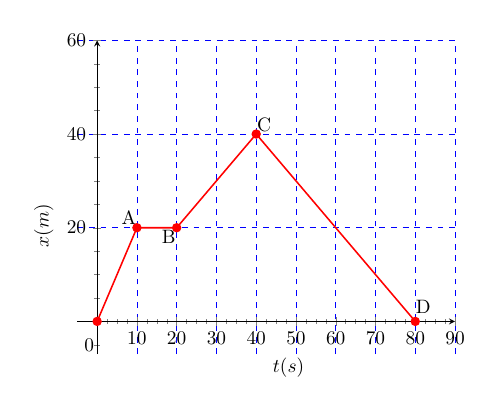
\begin{tikzpicture}[scale=0.7]
                \begin{axis}
                    [axis lines = left,
                    axis x line=center,
                    axis y line=center,
                    xlabel={$t(s)$},
                    ylabel={$x(m)$},
                    ylabel near ticks,
                    xlabel near ticks,
                    xlabel style={below right},
                    ylabel style={above left},
                    ymax=60,
                    ymin=-7,
                    xmax=90,
                    xmin=-5,
                    xtick={0,10,20,30,40,50,60,70,80,90},
                    ymajorgrids=true,
                    xmajorgrids=true,
                    minor tick num=3,
                    grid style={dashed, blue},
                    ]
                    \addplot[red,draw,thick, mark=*, mark options={fill=red}] coordinates {(0,0) (10,20) (20,20) (40,40) (80,0)};
                    \node at (axis cs:8,22) {A};
                    \draw (axis cs:10,20) circle;
                    \node at (axis cs:18,18) {B};
                    \node at (axis cs:42,42) {C};
                    \node at (axis cs:82,3) {D};
                    \node at (axis cs:-2,-5) {0};
                \end{axis}
        \end{tikzpicture}
        \caption{\textbf{Sistema de referencia}. Posición frente a tiempo.}
    \end{figure}
\end{minipage}
% Additional text translation
\vspace*{-6pt}
\begin{itemize}[leftmargin=0pt]
        \item En \( t_B=\qty{20}{\s} \), el ciclista está también en \( x_B = \qty{20}{\metre} \).
        Desde \( t_B=10 \) hasta \( t_C=20 \), el desplazamiento es \qty{0}{\m}, pero el desplazamiento total desde \( x_0 = 0 \) hasta \( x_B = 20 \) es \qty{20}{\m}.
        \item Desde \( x_C = 40 \) hasta \( x_D=0 \), la pendiente de la recta es negativa, lo que indica movimiento hacia atrás.
        El desplazamiento desde \( x_C = 40 \) hasta \( x_D = 0 \) es \qty{40}{\m} hacia atrás.
        Desde \( x_0 = 0 \) hasta \( x_D=80 \), el desplazamiento total es \qty{0}{\m}.
        \item La distancia total recorrida es la suma de cada tramo: \( 20 + 0 + 20 + 40 = \qty{80}{\m} \).
\end{itemize}

\textbf{Análisis del movimiento en cada tramo}:
\begin{itemize}
    \item Tramo 0-A: MRU (línea recta en la gráfica posición-tiempo)
    \item Tramo A-B: Sin movimiento (objeto en reposo)
    \item Tramo B-C: MRU de nuevo
    \item Tramo C-D: MRU hacia atrás
\end{itemize}
Las gráficas muestran la diferencia entre desplazamiento y distancia recorrida.
\section{Gráficas Velocidad-Tiempo}
Las gráficas velocidad-tiempo representan la velocidad de un objeto que se mueve durante un periodo de tiempo determinado.
\begin{figure}[H]
    \centering
    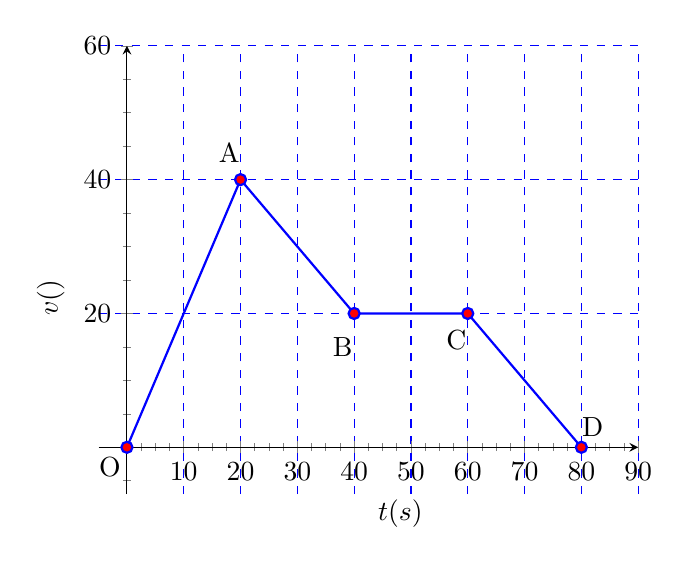
\begin{tikzpicture}[scale=1]
        \centering
        \begin{axis}
            [axis lines = left,
            axis x line=center,
            axis y line=center,
            mark=circle,
            xlabel={$t(s)$},
            ylabel={$v(\unit{\mps})$},
            ylabel near ticks,
            xlabel near ticks,
            xlabel style={below right},
            ylabel style={above left},
            ymax=60,
            ymin=-7,
            xmax=90,
            xmin=-5,
            xtick={0,10,20,30,40,50,60,70,80,90},
            ymajorgrids=true,
            xmajorgrids=true,
            minor tick num=3,
            grid style={dashed, blue},
            ]
            \addplot[blue,draw,thick, mark=*, mark options={fill=red}] coordinates {(0,0) (20,40) (40,20) (60,20) (80,0)};
            \node at (axis cs:18,44) {A};
            \draw (axis cs:10,20) circle;
            \node at (axis cs:38,15) {B};
            \node at (axis cs:58,16) {C};
            \node at (axis cs:82,3) {D};
            \node at (axis cs:-3,-3) {O};
        \end{axis}
    \end{tikzpicture}
    \caption{Gráfica de \( v \) frente a \( t \)}
\end{figure}

\textbf{Análisis del tipo de movimiento en los distintos tramos:}

\begin{itemize}
    \item Tramo O-A: Tenemos un movimiento rectilíneo uniformemente acelerado (MRUA) porque la gráfica velocidad-tiempo es una línea recta, y avanza hacia adelante.
    \item Tramo A-B: También tenemos MRUA, pero ahora moviéndose hacia atrás.
    \item Tramo B-C: Tenemos de nuevo un movimiento rectilíneo uniforme (MRU) porque la velocidad no cambia, por lo que la gráfica es horizontal.
    \item Tramo C-D: Otro MRUA, ahora moviéndose hacia atrás.
\end{itemize}


\begin{exercise}
    La siguiente gráfica muestra el movimiento de un objeto. Responde a las siguientes preguntas:
    \begin{enumerate}[label=\letraminuscula]
    \item ¿Qué tipo de movimiento se produce en cada tramo de la gráfica?
    \item Calcula la aceleración en cada tramo.
    \item ¿Cuál es la distancia total recorrida por el objeto?
    \end{enumerate}

    \begin{figure}[H]
        \centering
        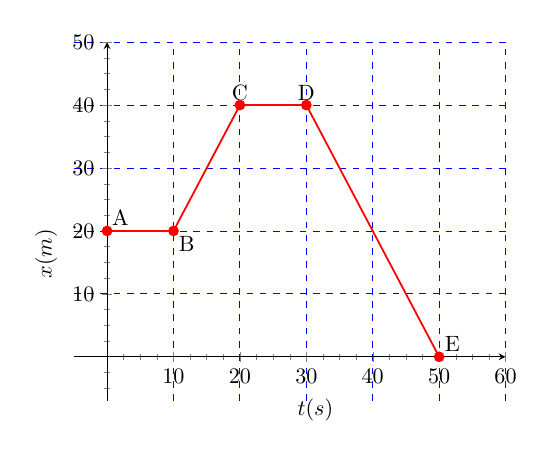
\begin{tikzpicture}[scale=0.8]
                \centering
                \begin{axis}
                    [axis lines = left,
                    axis x line=center,
                    axis y line=center,
                    mark=circle,
                    xlabel={$t(s)$},
                    ylabel={$x(m)$},
                    ylabel near ticks,
                    xlabel near ticks,
                    xlabel style={below right},
                    ylabel style={above left},
                    ymax=50,
                    ymin=-7,
                    xmax=60,
                    xmin=-5,
                    xtick={0,10,20,30,40,50,60},
                    ymajorgrids=true,
                    xmajorgrids=true,
                    minor tick num=3,
                    grid style={dashed, blue},
                    ]
                    \addplot[red,draw,thick, mark=*, mark options={fill=red}] coordinates {(0,20) (10,20) (20,40) (30,40) (50,0)};
                    \node at (axis cs:2,22) {A};
                    \draw (axis cs:10,20) circle;
                    \node at (axis cs:12,18) {B};
                    \node at (axis cs:20,42) {C};
                    \node at (axis cs:30,42) {D};
                    \node at (axis cs:52,2) {E};
                \end{axis}
        \end{tikzpicture}
    \end{figure}

    \begin{solu}
        \textbf{\textcolor{purple}{Ejercicio:}} La siguiente gráfica muestra el movimiento de un objeto. Responde a las siguientes preguntas:
        \begin{enumerate}[label=\letraminuscula]
            \item ¿Qué tipo de movimiento se produce en cada tramo de la gráfica?
            \item Calcula la aceleración en cada tramo.
            \item ¿Cuál es la distancia total recorrida por el objeto?
        \end{enumerate}

        \vspace{0.3cm}

        \textcolor{blue}{Lectura de la gráfica:}
        \begin{itemize}
            \item Punto A: $(0, 20)$ m
            \item Punto B: $(10, 20)$ m
            \item Punto C: $(20, 40)$ m
            \item Punto D: $(30, 40)$ m
            \item Punto E: $(50, 0)$ m
        \end{itemize}

        \textbf{\textcolor{blue}{Apartado a) Tipo de movimiento en cada tramo}}

        \textcolor{blue}{Tramo A-B ($t = 0$ a $t = 10$ s):}
        \begin{itemize}
            \item La posición permanece constante en 20 m
            \item \textcolor{red}{Tipo: En reposo (sin movimiento, $v = 0$)}
        \end{itemize}

        \textcolor{blue}{Tramo B-C ($t = 10$ a $t = 20$ s):}
        \begin{itemize}
            \item La posición aumenta linealmente de 20 m a 40 m
            \item \textcolor{red}{Tipo: Movimiento uniforme (velocidad positiva constante)}
        \end{itemize}

        \textcolor{blue}{Tramo C-D ($t = 20$ a $t = 30$ s):}
        \begin{itemize}
            \item La posición permanece constante en 40 m
            \item \textcolor{red}{Tipo: En reposo (sin movimiento, $v = 0$)}
        \end{itemize}

        \textcolor{blue}{Tramo D-E ($t = 30$ a $t = 50$ s):}
        \begin{itemize}
            \item La posición disminuye linealmente de 40 m a 0 m
            \item \textcolor{red}{Tipo: Movimiento uniforme (velocidad negativa constante - moviéndose hacia atrás)}
        \end{itemize}

        \vspace{0.5cm}

        \textbf{\textcolor{blue}{Apartado b) Calcular la aceleración en cada tramo}}

        \textcolor{red}{Concepto clave:} La aceleración es la tasa de cambio de la velocidad. En las gráficas posición-tiempo, la aceleración está relacionada con la curvatura de la gráfica.

        \textcolor{blue}{Tramo A-B:}
        \[
            v = \frac{\Delta x}{\Delta t} = \frac{20 - 20}{10 - 0} = 0 \text{ m/s}
        \]
        La velocidad es constante (cero), por lo que: $\textcolor{red}{a = 0 \text{ m/s}^2}$

        \textcolor{blue}{Tramo B-C:}
        \[
            v = \frac{\Delta x}{\Delta t} = \frac{40 - 20}{20 - 10} = \frac{20}{10} = 2 \text{ m/s}
        \]
        La velocidad es constante, por lo que: $\textcolor{red}{a = 0 \text{ m/s}^2}$

        \textcolor{blue}{Tramo C-D:}
        \[
            v = \frac{\Delta x}{\Delta t} = \frac{40 - 40}{30 - 20} = 0 \text{ m/s}
        \]
        La velocidad es constante (cero), por lo que: $\textcolor{red}{a = 0 \text{ m/s}^2}$

        \textcolor{blue}{Tramo D-E:}
        \[
            v = \frac{\Delta x}{\Delta t} = \frac{0 - 40}{50 - 30} = \frac{-40}{20} = -2 \text{ m/s}
        \]
        La velocidad es constante, por lo que: $\textcolor{red}{a = 0 \text{ m/s}^2}$

        \textcolor{red}{Resumen:} La aceleración es \textbf{cero} en todos los tramos porque la gráfica está formada por segmentos de línea recta (velocidad constante en cada tramo). La velocidad cambia \textit{instantáneamente} en los puntos B, C y D, lo que requeriría una aceleración infinita, pero esto es una idealización.

        \vspace{0.5cm}

        \textbf{\textcolor{blue}{Apartado c) Distancia total recorrida}}

        \textcolor{red}{Importante:} La distancia es la longitud total del camino recorrido (siempre positiva), independientemente de la dirección.

        \textcolor{blue}{Tramo A-B:}
        \[
            d_{AB} = |20 - 20| = 0 \text{ m}
        \]

        \textcolor{blue}{Tramo B-C:}
        \[
            d_{BC} = |40 - 20| = 20 \text{ m}
        \]

        \textcolor{blue}{Tramo C-D:}
        \[
            d_{CD} = |40 - 40| = 0 \text{ m}
        \]

        \textcolor{blue}{Tramo D-E:}
        \[
            d_{DE} = |0 - 40| = 40 \text{ m}
        \]

        \textcolor{blue}{Distancia total:}
        \[
            d_{\text{total}} = d_{AB} + d_{BC} + d_{CD} + d_{DE}
        \]
        \[
            d_{\text{total}} = 0 + 20 + 0 + 40 = \textcolor{red}{60 \text{ m}}
        \]

        \textcolor{red}{Respuesta c):} La distancia total recorrida por el objeto es \textbf{60 m}.

        \textcolor{blue}{Nota:} El desplazamiento (cambio de posición entre el inicio y el final) sería $0 - 20 = -20$ m, que es diferente de la distancia total recorrida.
    \end{solu}
\end{exercise}

\begin{exercise}
    La siguiente gráfica muestra el movimiento de un objeto. Responde a las siguientes preguntas:
    \begin{enumerate}[label=\letraminuscula]
    \item ¿Qué tipo de movimiento se produce en cada tramo de la gráfica?
    \item Calcula la aceleración en cada tramo.
    \item ¿Cuál es la distancia total recorrida por el objeto?
    \end{enumerate}

    \begin{figure}[H]
        \centering
        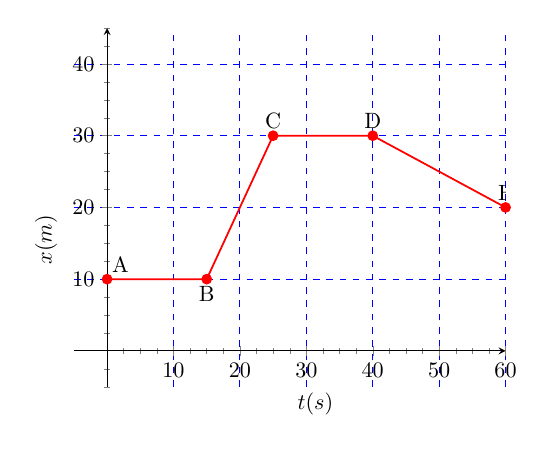
\begin{tikzpicture}[scale=0.8]
                \centering
                \begin{axis}
                    [axis lines = left,
                    axis x line=center,
                    axis y line=center,
                    xlabel={$t(s)$},
                    ylabel={$x(m)$},
                    ylabel near ticks,
                    xlabel near ticks,
                    xlabel style={below right},
                    ylabel style={above left},
                    ymax=45,
                    ymin=-5,
                    xmax=60,
                    xmin=-5,
                    xtick={0,10,20,30,40,50,60},
                    ymajorgrids=true,
                    xmajorgrids=true,
                    minor tick num=3,
                    grid style={dashed, blue},
                    ]
                    \addplot[red,draw,thick, mark=*, mark options={fill=red}] coordinates {(0,10) (15,10) (25,30) (40,30) (60,20)};
                    \node at (axis cs:2,12) {A};
                    \node at (axis cs:15,8) {B};
                    \node at (axis cs:25,32) {C};
                    \node at (axis cs:40,32) {D};
                    \node at (axis cs:60,22) {E};
                \end{axis}
        \end{tikzpicture}
    \end{figure}

    \begin{solu}
        \textbf{\textcolor{purple}{Ejercicio:}} La siguiente gráfica muestra el movimiento de un objeto. Responde a las siguientes preguntas:
        \begin{enumerate}[label=\letraminuscula]
            \item ¿Qué tipo de movimiento se produce en cada tramo de la gráfica?
            \item Calcula la aceleración en cada tramo.
            \item ¿Cuál es la distancia total recorrida por el objeto?
        \end{enumerate}

        \vspace{0.3cm}

        \textcolor{blue}{Lectura de la gráfica:}
        \begin{itemize}
            \item Punto A: $(0,10)$ m
            \item Punto B: $(15,10)$ m
            \item Punto C: $(25,30)$ m
            \item Punto D: $(40,30)$ m
            \item Punto E: $(60,20)$ m
        \end{itemize}

        \textbf{\textcolor{blue}{Apartado a) Tipo de movimiento en cada tramo}}

        \textcolor{blue}{Tramo A-B ($t=0$ a $15$ s):}
        \begin{itemize}
            \item La posición permanece constante.
            \item \textcolor{red}{Tipo: En reposo ($v=0$).}
        \end{itemize}

        \textcolor{blue}{Tramo B-C ($t=15$ a $25$ s):}
        \begin{itemize}
            \item La posición aumenta linealmente.
            \item \textcolor{red}{Tipo: Movimiento uniforme (velocidad positiva constante).}
        \end{itemize}

        \textcolor{blue}{Tramo C-D ($t=25$ a $40$ s):}
        \begin{itemize}
            \item La posición permanece constante.
            \item \textcolor{red}{Tipo: En reposo ($v=0$).}
        \end{itemize}

        \textcolor{blue}{Tramo D-E ($t=40$ a $60$ s):}
        \begin{itemize}
            \item La posición disminuye linealmente.
            \item \textcolor{red}{Tipo: Movimiento uniforme (velocidad negativa constante).}
        \end{itemize}

        \vspace{0.5cm}

        \textbf{\textcolor{blue}{Apartado b) Calcular la aceleración en cada tramo}}

        \textcolor{blue}{Tramo A-B:}
        \[
        v=\frac{10-10}{15-0}=0\text{ m/s}
        \]
        Por lo tanto,
        \[
        \boxed{a=0\text{ m/s}^2}
        \]

        \textcolor{blue}{Tramo B-C:}
        \[
        v=\frac{30-10}{25-15}=\frac{20}{10}=2\text{ m/s}
        \]
        Por lo tanto,
        \[
        \boxed{a=0\text{ m/s}^2}
        \]

        \textcolor{blue}{Tramo C-D:}
        \[
        v=\frac{30-30}{40-25}=0\text{ m/s}
        \]
        Por lo tanto,
        \[
        \boxed{a=0\text{ m/s}^2}
        \]

        \textcolor{blue}{Tramo D-E:}
        \[
        v=\frac{20-30}{60-40}=\frac{-10}{20}=-0.5\text{ m/s}
        \]
        Por lo tanto,
        \[
        \boxed{a=0\text{ m/s}^2}
        \]

        \textcolor{red}{La aceleración es cero en todos los tramos porque la velocidad es constante en cada intervalo.}

        \vspace{0.5cm}

        \textbf{\textcolor{blue}{Apartado c) Distancia total recorrida}}

        \[
        d_{AB}=0\text{ m}
        \]

        \[
        d_{BC}=20\text{ m}
        \]

        \[
        d_{CD}=0\text{ m}
        \]

        \[
        d_{DE}=10\text{ m}
        \]

        \[
        d_{\text{total}}=0+20+0+10=\boxed{30\text{ m}}
        \]

        \textcolor{blue}{El desplazamiento es $20-10=10$ m.}
    \end{solu}
\end{exercise}

\begin{exercise}
    La siguiente gráfica muestra el movimiento de un objeto. Responde a las siguientes preguntas:
    \begin{enumerate}[label=\letraminuscula]
    \item ¿Qué tipo de movimiento se produce en cada tramo de la gráfica?
    \item Calcula la aceleración en cada tramo.
    \item ¿Cuál es la distancia total recorrida por el objeto?
    \end{enumerate}

    \begin{figure}[H]
        \centering
        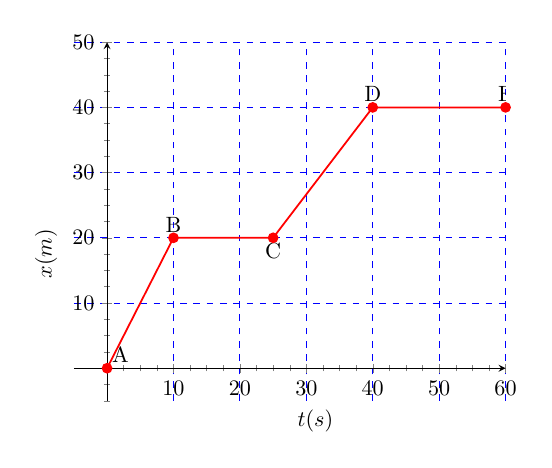
\begin{tikzpicture}[scale=0.8]
                \centering
                \begin{axis}
                    [axis lines = left,
                    axis x line=center,
                    axis y line=center,
                    xlabel={$t(s)$},
                    ylabel={$x(m)$},
                    ylabel near ticks,
                    xlabel near ticks,
                    xlabel style={below right},
                    ylabel style={above left},
                    ymax=50,
                    ymin=-5,
                    xmax=60,
                    xmin=-5,
                    xtick={0,10,20,30,40,50,60},
                    ymajorgrids=true,
                    xmajorgrids=true,
                    minor tick num=3,
                    grid style={dashed, blue},
                    ]
                    \addplot[red,draw,thick, mark=*, mark options={fill=red}] coordinates {(0,0) (10,20) (25,20) (40,40) (60,40)};
                    \node at (axis cs:2,2) {A};
                    \node at (axis cs:10,22) {B};
                    \node at (axis cs:25,18) {C};
                    \node at (axis cs:40,42) {D};
                    \node at (axis cs:60,42) {E};
                \end{axis}
        \end{tikzpicture}
    \end{figure}

    \begin{solu}
        \textbf{\textcolor{purple}{Ejercicio:}} La siguiente gráfica muestra el movimiento de un objeto. Responde a las siguientes preguntas:
        \begin{enumerate}[label=\letraminuscula]
            \item ¿Qué tipo de movimiento se produce en cada tramo de la gráfica?
            \item Calcula la aceleración en cada tramo.
            \item ¿Cuál es la distancia total recorrida por el objeto?
        \end{enumerate}

        \vspace{0.3cm}

        \textcolor{blue}{Lectura de la gráfica:}
        \begin{itemize}
            \item Punto A: $(0,0)$ m
            \item Punto B: $(10,20)$ m
            \item Punto C: $(25,20)$ m
            \item Punto D: $(40,40)$ m
            \item Punto E: $(60,40)$ m
        \end{itemize}

        \textbf{\textcolor{blue}{Apartado a) Tipo de movimiento en cada tramo}}

        \textcolor{blue}{Tramo A-B:}
        \begin{itemize}
            \item La posición aumenta linealmente.
            \item \textcolor{red}{Tipo: Movimiento uniforme (velocidad positiva constante).}
        \end{itemize}

        \textcolor{blue}{Tramo B-C:}
        \begin{itemize}
            \item La posición permanece constante.
            \item \textcolor{red}{Tipo: En reposo.}
        \end{itemize}

        \textcolor{blue}{Tramo C-D:}
        \begin{itemize}
            \item La posición aumenta linealmente.
            \item \textcolor{red}{Tipo: Movimiento uniforme (velocidad positiva constante).}
        \end{itemize}

        \textcolor{blue}{Tramo D-E:}
        \begin{itemize}
            \item La posición permanece constante.
            \item \textcolor{red}{Tipo: En reposo.}
        \end{itemize}

        \vspace{0.5cm}

        \textbf{\textcolor{blue}{Apartado b) Calcular la aceleración en cada tramo}}

        \textcolor{blue}{Tramo A-B:}
        \[
        v=\frac{20-0}{10-0}=2\text{ m/s}
        \]
        Por lo tanto,
        \[
        \boxed{a=0\text{ m/s}^2}
        \]

        \textcolor{blue}{Tramo B-C:}
        \[
        v=\frac{20-20}{25-10}=0\text{ m/s}
        \]
        Por lo tanto,
        \[
        \boxed{a=0\text{ m/s}^2}
        \]

        \textcolor{blue}{Tramo C-D:}
        \[
        v=\frac{40-20}{40-25}=\frac{20}{15}=1.33\text{ m/s}
        \]
        Por lo tanto,
        \[
        \boxed{a=0\text{ m/s}^2}
        \]

        \textcolor{blue}{Tramo D-E:}
        \[
        v=\frac{40-40}{60-40}=0\text{ m/s}
        \]
        Por lo tanto,
        \[
        \boxed{a=0\text{ m/s}^2}
        \]

        \textcolor{red}{La aceleración es cero en todos los tramos porque cada segmento es una línea recta.}

        \vspace{0.5cm}

        \textbf{\textcolor{blue}{Apartado c) Distancia total recorrida}}

        \[
        d_{AB}=20\text{ m}
        \]

        \[
        d_{BC}=0\text{ m}
        \]

        \[
        d_{CD}=20\text{ m}
        \]

        \[
        d_{DE}=0\text{ m}
        \]

        \[
        d_{\text{total}}=20+0+20+0=\boxed{40\text{ m}}
        \]

        \textcolor{blue}{El desplazamiento es $40-0=40$ m.}
    \end{solu}
\end{exercise}

\begin{exercise}
    La siguiente gráfica muestra la velocidad de un objeto. Responde a las siguientes preguntas:
    \begin{enumerate}[label=\letraminuscula]
    \item ¿Qué tipo de movimiento se produce en cada tramo de la gráfica?
    \item Calcula la aceleración en cada tramo.
    \item ¿Cuál es la distancia total recorrida por el objeto?
    \end{enumerate}

    \begin{figure}[H]
        \centering
        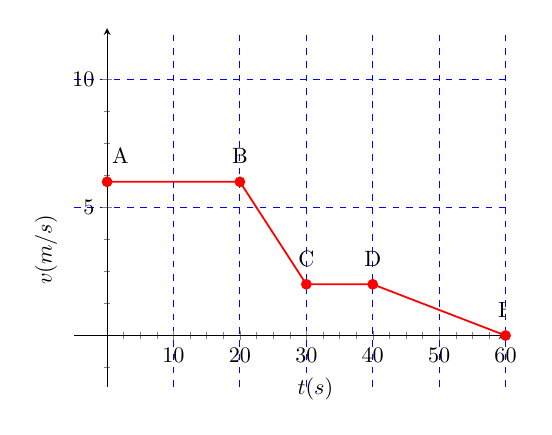
\begin{tikzpicture}[scale=0.8]
            \begin{axis}
                [axis lines = left,
                axis x line=center,
                axis y line=center,
                xlabel={$t(s)$},
                ylabel={$v(m/s)$},
                ylabel near ticks,
                xlabel near ticks,
                xlabel style={below right},
                ylabel style={above left},
                ymax=12,
                ymin=-2,
                xmax=60,
                xmin=-5,
                xtick={0,10,20,30,40,50,60},
                ymajorgrids=true,
                xmajorgrids=true,
                minor tick num=3,
                grid style={dashed, blue},
                ]
                \addplot[red,draw,thick,mark=*,mark options={fill=red}]
                coordinates {(0,6) (20,6) (30,2) (40,2) (60,0)};
                \node at (axis cs:2,7) {A};
                \node at (axis cs:20,7) {B};
                \node at (axis cs:30,3) {C};
                \node at (axis cs:40,3) {D};
                \node at (axis cs:60,1) {E};
            \end{axis}
        \end{tikzpicture}
    \end{figure}

    \begin{solu}

    \textbf{\textcolor{purple}{Ejercicio:}} La siguiente gráfica muestra la velocidad de un objeto.

    \textcolor{blue}{Lectura de la gráfica:}
    \begin{itemize}
        \item A: $(0,6)$ m/s
        \item B: $(20,6)$ m/s
        \item C: $(30,2)$ m/s
        \item D: $(40,2)$ m/s
        \item E: $(60,0)$ m/s
    \end{itemize}

    \textbf{\textcolor{blue}{Apartado a) Tipo de movimiento}}

    \textbf{A-B:}
    \begin{itemize}
        \item Velocidad constante.
        \item \textcolor{red}{Movimiento uniforme.}
    \end{itemize}

    \textbf{B-C:}
    \begin{itemize}
        \item La velocidad disminuye de manera uniforme.
        \item \textcolor{red}{Movimiento uniformemente decelerado.}
    \end{itemize}

    \textbf{C-D:}
    \begin{itemize}
        \item Velocidad constante.
        \item \textcolor{red}{Movimiento uniforme.}
    \end{itemize}

    \textbf{D-E:}
    \begin{itemize}
        \item La velocidad disminuye de manera uniforme.
        \item \textcolor{red}{Movimiento uniformemente decelerado.}
    \end{itemize}

    \textbf{\textcolor{blue}{Apartado b) Aceleración}}

    A-B:
    \[
    a=\frac{6-6}{20}=0\text{ m/s}^2
    \]

    B-C:
    \[
    a=\frac{2-6}{10}=-0.4\text{ m/s}^2
    \]

    C-D:
    \[
    a=\frac{2-2}{10}=0\text{ m/s}^2
    \]

    D-E:
    \[
    a=\frac{0-2}{20}=-0.1\text{ m/s}^2
    \]

    \textbf{\textcolor{blue}{Apartado c) Distancia total}}

    Área A-B:
    \[
    (20)(6)=120\text{ m}
    \]

    Área B-C:
    \[
    \frac{6+2}{2}(10)=40\text{ m}
    \]

    Área C-D:
    \[
    (10)(2)=20\text{ m}
    \]

    Área D-E:
    \[
    \frac{2+0}{2}(20)=20\text{ m}
    \]

    Distancia total:
    \[
    d=120+40+20+20=\boxed{200\text{ m}}
    \]

    \end{solu}
\end{exercise}

\begin{exercise}
    La siguiente gráfica muestra la velocidad de un objeto. Responde a las siguientes preguntas:
    \begin{enumerate}[label=\letraminuscula]
    \item ¿Qué tipo de movimiento se produce en cada tramo de la gráfica?
    \item Calcula la aceleración en cada tramo.
    \item ¿Cuál es la distancia total recorrida por el objeto?
    \end{enumerate}

    \begin{figure}[H]
        \centering
        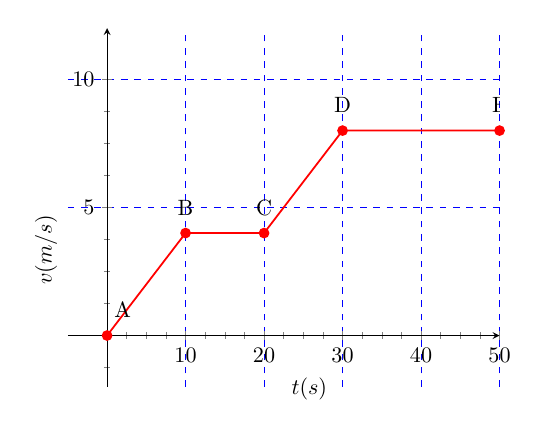
\begin{tikzpicture}[scale=0.8]
            \begin{axis}
                [axis lines = left,
                axis x line=center,
                axis y line=center,
                xlabel={$t(s)$},
                ylabel={$v(m/s)$},
                ylabel near ticks,
                xlabel near ticks,
                xlabel style={below right},
                ylabel style={above left},
                ymax=12,
                ymin=-2,
                xmax=50,
                xmin=-5,
                xtick={0,10,20,30,40,50},
                ymajorgrids=true,
                xmajorgrids=true,
                minor tick num=3,
                grid style={dashed, blue},
                ]
                \addplot[red,draw,thick,mark=*,mark options={fill=red}]
                coordinates {(0,0) (10,4) (20,4) (30,8) (50,8)};
                \node at (axis cs:2,1) {A};
                \node at (axis cs:10,5) {B};
                \node at (axis cs:20,5) {C};
                \node at (axis cs:30,9) {D};
                \node at (axis cs:50,9) {E};
            \end{axis}
        \end{tikzpicture}
    \end{figure}

    \begin{solu}

    \textbf{\textcolor{purple}{Ejercicio:}} La siguiente gráfica muestra la velocidad de un objeto.

    \textcolor{blue}{Lectura de la gráfica:}
    \begin{itemize}
        \item A: $(0,0)$ m/s
        \item B: $(10,4)$ m/s
        \item C: $(20,4)$ m/s
        \item D: $(30,8)$ m/s
        \item E: $(50,8)$ m/s
    \end{itemize}

    \textbf{\textcolor{blue}{Apartado a) Tipo de movimiento}}

    \textbf{A-B:}
    \begin{itemize}
        \item La velocidad aumenta de manera uniforme.
        \item \textcolor{red}{Movimiento uniformemente acelerado.}
    \end{itemize}

    \textbf{B-C:}
    \begin{itemize}
        \item Velocidad constante.
        \item \textcolor{red}{Movimiento uniforme.}
    \end{itemize}

    \textbf{C-D:}
    \begin{itemize}
        \item La velocidad aumenta de manera uniforme.
        \item \textcolor{red}{Movimiento uniformemente acelerado.}
    \end{itemize}

    \textbf{D-E:}
    \begin{itemize}
        \item Velocidad constante.
        \item \textcolor{red}{Movimiento uniforme.}
    \end{itemize}

    \textbf{\textcolor{blue}{Apartado b) Aceleración}}

    A-B:
    \[
    a=\frac{4-0}{10}=0.4\text{ m/s}^2
    \]

    B-C:
    \[
    a=\frac{4-4}{10}=0\text{ m/s}^2
    \]

    C-D:
    \[
    a=\frac{8-4}{10}=0.4\text{ m/s}^2
    \]

    D-E:
    \[
    a=\frac{8-8}{20}=0\text{ m/s}^2
    \]

    \textbf{\textcolor{blue}{Apartado c) Distancia total}}

    Área A-B:
    \[
    \frac12(10)(4)=20\text{ m}
    \]

    Área B-C:
    \[
    (10)(4)=40\text{ m}
    \]

    Área C-D:
    \[
    \frac{4+8}{2}(10)=60\text{ m}
    \]

    Área D-E:
    \[
    (20)(8)=160\text{ m}
    \]

    Distancia total:
    \[
    d=20+40+60+160=\boxed{280\text{ m}}
    \]

    \end{solu}
\end{exercise}

\begin{exercise}
    Elabora un mapa conceptual que resuma los principales temas de esta unidad.
    \begin{solu}
        \textbf{\textcolor{purple}{Ejercicio:}} Elabora un mapa conceptual que resuma los principales temas de esta unidad.

        \textcolor{blue}{Este es un ejercicio abierto en el que el alumnado debe crear su propio mapa conceptual incluyendo términos clave como: posición, desplazamiento, velocidad, rapidez, aceleración, movimiento uniforme, movimiento uniformemente acelerado, gráficas posición-tiempo, gráficas velocidad-tiempo, ecuaciones cinemáticas, etc.}
    \end{solu}
\end{exercise}

%\section{Vocabulary}
%
%\begin{vocabulary}[Kinematics]
%The branch of Physics that studies motion without taking into account the causes that produce it. It focuses on describing how objects move through space and time. \newline
%\textbf{Translation to Spanish}: Cinemática \newline
%% Line 9
%\end{vocabulary}
%
%\begin{vocabulary}[Motion]
%The change in position of an object with respect to a reference system over time. An object is in motion when its position changes relative to a chosen reference point. \newline
%\textbf{Translation to Spanish}: Movimiento \newline
%% Line 49
%\end{vocabulary}
%
%\begin{vocabulary}[Rest]
%The state of an object when its position does not change with respect to a reference system over time. \newline
%\textbf{Translation to Spanish}: Reposo \newline
%% Line 51
%\end{vocabulary}
%
%\begin{vocabulary}[Reference System]
%A system that allows us to fix the position of an object and study its evolution over time. In Physics, it is usually a Cartesian coordinate system (x, y). \newline
%\textbf{Translation to Spanish}: Sistema de referencia \newline
%% Line 58
%\end{vocabulary}
%
%\begin{vocabulary}[Position]
%The exact location of an object in space, usually represented by the letter x. The SI unit is the meter (m). \newline
%\textbf{Translation to Spanish}: Posición \newline
%% Line 69
%\end{vocabulary}
%
%\begin{vocabulary}[Displacement]
%The difference between the final position and the initial position of the motion, represented as \( \Delta x = x_f - x_i \). It is a vector quantity that can be positive or negative. The SI unit is the meter (m). \newline
%\textbf{Translation to Spanish}: Desplazamiento \newline
%% Line 73
%\end{vocabulary}
%
%\begin{vocabulary}[Trajectory]
%The path followed by an object during its motion. It can be rectilinear (straight line), circular, or curvilinear (curved). \newline
%\textbf{Translation to Spanish}: Trayectoria \newline
%% Line 103
%\end{vocabulary}
%
%\begin{vocabulary}[Distance Travelled]
%The length of the trajectory followed by an object. It is a scalar quantity always positive. The SI unit is the meter (m). \newline
%\textbf{Translation to Spanish}: Distancia recorrida \newline
%% Line 106
%\end{vocabulary}
%
%\begin{vocabulary}[Rectilinear Motion]
%Motion in which the trajectory is a straight line. In this type of motion, displacement coincides with the distance traveled. \newline
%\textbf{Translation to Spanish}: Movimiento rectilíneo \newline
%% Line 114
%\end{vocabulary}
%
%\begin{vocabulary}[Circular Motion]
%Motion in which the trajectory is circular or describes a circle. \newline
%\textbf{Translation to Spanish}: Movimiento circular \newline
%% Line 117
%\end{vocabulary}
%
%\begin{vocabulary}[Curvilinear Motion]
%Motion in which the trajectory describes curves that are neither straight lines nor perfect circles. \newline
%\textbf{Translation to Spanish}: Movimiento curvilíneo \newline
%% Line 119
%\end{vocabulary}
%
%\begin{vocabulary}[Velocity]
%The rate of change of position with respect to time. It is a vector quantity that indicates both speed and direction. The SI unit is meters per second (m/s). \newline
%\textbf{Translation to Spanish}: Velocidad \newline
%% Line 201 (approximately, appears throughout the document)
%\end{vocabulary}
%
%\begin{vocabulary}[Speed]
%The magnitude of velocity, representing how fast an object is moving without regard to direction. It is a scalar quantity. The SI unit is meters per second (m/s). \newline
%\textbf{Translation to Spanish}: Rapidez \newline
%% Line 201 (approximately, appears throughout the document)
%\end{vocabulary}
%
%\begin{vocabulary}[Average Velocity]
%The total displacement divided by the total time taken. It is calculated as \( v_{avg} = \Delta x / \Delta t \) \newline
%\textbf{Translation to Spanish}: Velocidad media \newline
%% Line 201 (approximately, appears in context)
%\end{vocabulary}
%
%\begin{vocabulary}[Instantaneous Velocity]
%The velocity of an object at a specific instant of time. It is the limit of average velocity as the time interval approaches zero. \newline
%\textbf{Translation to Spanish}: Velocidad instantánea \newline
%% Line 201 (approximately, appears in context)
%\end{vocabulary}
%
%\begin{vocabulary}[Acceleration]
%The rate of change of velocity with respect to time. It is a vector quantity. The SI unit is meters per second squared (m/s²). \newline
%\textbf{Translation to Spanish}: Aceleración \newline
%% Line 201 (approximately, appears throughout the document)
%\end{vocabulary}
%
%\begin{vocabulary}[Uniform Rectilinear Motion (URM)]
%Motion in a straight line with constant velocity (zero acceleration). The object covers equal distances in equal time intervals. \newline
%\textbf{Translation to Spanish}: Movimiento rectilíneo uniforme (MRU) \newline
%% Line 2346
%\end{vocabulary}
%
%\begin{vocabulary}[Uniformly Accelerated Rectilinear Motion (UARM)]
%Motion in a straight line with constant acceleration. The velocity changes uniformly over time. Also known as uniformly varied motion. \newline
%\textbf{Translation to Spanish}: Movimiento rectilíneo uniformemente acelerado (MRUA) \newline
%% Line 2399
%\end{vocabulary}
%
%\begin{vocabulary}[Coordinate System]
%A system used to specify the position of a point in space using numerical coordinates. The most common is the Cartesian coordinate system. \newline
%\textbf{Translation to Spanish}: Sistema de coordenadas \newline
%% Line 55
%\end{vocabulary}
%
%\begin{vocabulary}[Origin]
%The reference point in a coordinate system where all coordinates are zero. It serves as the starting point for measuring position. \newline
%\textbf{Translation to Spanish}: Origen \newline
%% Line 2288
%\end{vocabulary}
%
%\begin{vocabulary}[Time Interval]
%The difference between two moments in time, calculated as \( \Delta t = t_f - t_i \). It represents the duration of an event or motion. \newline
%\textbf{Translation to Spanish}: Intervalo de tiempo \newline
%% Line 94
%\end{vocabulary}
%
%\begin{vocabulary}[Position-Time Graph]
%A graphical representation showing how an object's position changes over time. The slope of the graph represents velocity. \newline
%\textbf{Translation to Spanish}: Gráfica posición-tiempo \newline
%% Line 2283
%\end{vocabulary}
%
%\begin{vocabulary}[Velocity-Time Graph]
%A graphical representation showing how an object's velocity changes over time. The slope represents acceleration, and the area under the curve represents displacement. \newline
%\textbf{Translation to Spanish}: Gráfica velocidad-tiempo \newline
%% Line 2355
%\end{vocabulary}
%
%\begin{vocabulary}[Slope]
%In a graph, the slope represents the rate of change of the vertical quantity with respect to the horizontal quantity. In position-time graphs, slope represents velocity; in velocity-time graphs, it represents acceleration. \newline
%\textbf{Translation to Spanish}: Pendiente \newline
%% Line 2337
%\end{vocabulary}
%
%\begin{vocabulary}[Vector Quantity]
%A physical quantity that has both magnitude and direction. Examples include displacement, velocity, and acceleration. \newline
%\textbf{Translation to Spanish}: Magnitud vectorial \newline
%% Line 159
%\end{vocabulary}
%
%\begin{vocabulary}[Scalar Quantity]
%A physical quantity that has only magnitude but no direction. Examples include distance, speed, and time. \newline
%\textbf{Translation to Spanish}: Magnitud escalar \newline
%% Line 107 (implied in context)
%\end{vocabulary}
%
%\begin{vocabulary}[Initial Position]
%The position of an object at the beginning of motion or at the start of observation, represented as \( x_i \) or \(v  \). \newline
%\textbf{Translation to Spanish}: Posición inicial \newline
%% Line 83
%\end{vocabulary}
%
%\begin{vocabulary}[Final Position]
%The position of an object at the end of motion or at a specific moment, represented as \( x_f \) . \newline
%\textbf{Translation to Spanish}: Posición final \newline
%% Line 81
%\end{vocabulary}
%
%\begin{vocabulary}[Cartesian Coordinate System]
%A coordinate system that uses perpendicular axes (typically x and y in 2D, or x, y, and z in 3D) to specify positions in space. \newline
%\textbf{Translation to Spanish}: Sistema de coordenadas cartesianas \newline
%% Line 55
%\end{vocabulary}
%
%\begin{vocabulary}[Frame of Reference]
%A perspective from which motion is observed and measured. Motion is relative and depends on the chosen frame of reference. \newline
%\textbf{Translation to Spanish}: Sistema de referencia \newline
%% Line 53
%\end{vocabulary}
%
%
%%\begin{exercise}
%%    Vocabulary
%%
%%    \begin{multicols}{2}
%%        \begin{enumerate}
%%            \item Acceleration
%%            \item at rest
%%            \item Average
%%            \item Axis
%%            \item Coordinate System
%%            \item Deform
%%            \item Direction
%%            \item displacement
%%            \item Frame of reference
%%            \item Instantaneous
%%            \item Interval
%%            \item Law
%%            \item Motion
%%            \item Origin
%%            \item Slope
%%            \item Speed
%%            \item Trajectory
%%            \item Uniform rectilinear motion.
%%        \end{enumerate}
%%    \end{multicols}
%
%%\end{exercise}
%
%
%
%
%
%


%------------------------------------------------


    \chapterimage{Images/portada_cabeceras/cabecera_U3_dinamica}
    \chapter{Dinámica}

    
%! Author = crist
%! Date = 03/07/2025

\spacing{1.3}


\section{Fuerzas}
\begin{definition}[Fuerza]
        Una \textbf{fuerza} es una magnitud física que representa cualquier acción capaz de modificar la forma de un cuerpo o cambiar el estado de reposo o movimiento de dicho cuerpo.
\end{definition}
La unidad de fuerza en el Sistema Internacional es el Newton (\unit{\newton}).
Podemos definir un Newton como la fuerza que produce en un cuerpo de un kilogramo una aceleración de un \unit{\mpss}.

En la naturaleza existen cuatro fuerzas fundamentales:
\begin{itemize}
    \item Fuerza gravitatoria.
    \item Fuerza electromagnética.
    \item Fuerza nuclear fuerte.
    \item Fuerza nuclear débil.
\end{itemize}

En este capítulo estudiaremos la fuerza gravitatoria y la fuerza electromagnética, que separaremos en fuerza eléctrica (dentro de la fuerza electromagnética).

\subsection{Partes de una fuerza: representación de una fuerza}

Para representar correctamente una fuerza, es necesario saber que tiene cuatro elementos:

\begin{itemize}
    \item \textbf{Punto de aplicación}.
    Es el lugar donde se aplica la fuerza.
    Se suele indicar con un punto, aunque es bastante habitual omitirlo.
    \item \textbf{Magnitud}.
    Indica la cantidad de fuerza que se aplica, es decir, el valor numérico.
    \item \textbf{Dirección}.
    Indica hacia dónde se aplica la fuerza (horizontal, vertical o inclinada) y se representa mediante una línea recta.
    Cuanto mayor sea la magnitud, más larga será la línea.
    \item \textbf{Sentido}.
    Muestra hacia qué lado apunta la fuerza y se representa con una punta de flecha.
    Numéricamente, el sentido se indica con un signo positivo o negativo.
    Siempre se elige una dirección; si la fuerza es positiva, significa que está dirigida hacia la dirección elegida, mientras que si es negativa, está dirigida en el sentido contrario.
\end{itemize}

\begin{figure}[H]
    \centering
    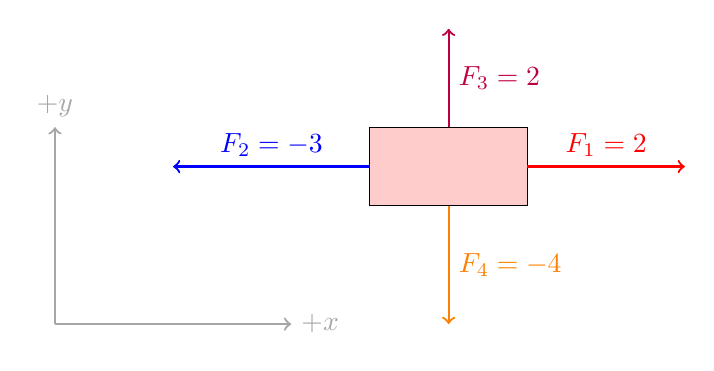
\begin{tikzpicture}

        % Positive axes
        \draw[->, thick, gray!70] (-4,-1.5) -- ++(0,2.5) node[above] {$+y$};
        \draw[->, thick, gray!70] (-4,-1.5) -- ++(3,0) node[right] {$+x$};

        % Block
        \draw[fill=red!20] (0,0) rectangle (2,1);

        % Force F1 (horizontal right)
        \draw[->, thick, red] (2,0.5) -- +(2,0)
        node[midway, above] {$F_1 = \qty{2}{\newton}$};

        % Force F2 (horizontal left)
        \draw[->, thick, blue] (0,0.5) -- +(-2.5,0)
        node[midway, above] {$F_2 = \qty{-3}{\newton}$};

        % Force F3 (vertical upward)
        \draw[->, thick, purple] (1,1) -- +(0,1.25)
        node[midway, right] {$F_3 = \qty{2}{\newton}$};

        % Force F4 (vertical downward)
        \draw[->, thick, orange] (1,0) -- +(0,-1.5)
        node[midway, right] {$F_4 = \qty{-4}{\newton}$};

    \end{tikzpicture}
    \caption{Representación de fuerzas}
    \label{fig:representacion_fuerzas}
\end{figure}

\begin{exercise}
    En tu cuaderno, dibuja las siguientes fuerzas, aplicadas en el origen de las coordenadas XY:
    \begin{enumerate}[label=\letraminuscula]
        \item una fuerza de 5 N, en dirección horizontal hacia la derecha.
        \item una fuerza igual a la anterior, pero en
        dirección opuesta.
        \item una fuerza vertical de 10 N, apuntando hacia arriba.
    \end{enumerate}
    \begin{solu}
        Los estudiantes deben dibujar un sistema de coordenadas con el origen en el centro, y luego dibujar tres vectores de fuerza:

        \textbf{a)} Dibuja una flecha apuntando hacia la derecha a lo largo del eje X positivo con magnitud 5 N. Etiquétala como $\vec{F}_1 = 5$ N.

        \textbf{b)} Dibuja una flecha apuntando hacia la izquierda a lo largo del eje X negativo con magnitud 5 N. Etiquétala como $\vec{F}_2 = -5$ N o $\vec{F}_2 = 5$ N hacia la izquierda.

        \textbf{c)} Dibuja una flecha apuntando hacia arriba a lo largo del eje Y positivo con magnitud 10 N. Etiquétala como $\vec{F}_3 = 10$ N.

        Las flechas deben dibujarse a escala, de modo que la fuerza de 10 N sea el doble de larga que las fuerzas de 5 N. Todas las fuerzas se originan en el origen del sistema de coordenadas.
    \end{solu}
\end{exercise}

\subsection{Operaciones con fuerzas: suma de fuerzas}

En Física, el símbolo \( \Sigma \) indica que se deben sumar todas las magnitudes presentes.
Si tenemos \( \Sigma F \), significa que debemos sumar todas las fuerzas que actúan sobre el objeto.

Podemos tener los siguientes casos:

\begin{itemize}
    \item \textbf{Fuerzas con el mismo sentido}.
    Ambas tendrán signo positivo.
    \begin{figure}[H]
        \centering
        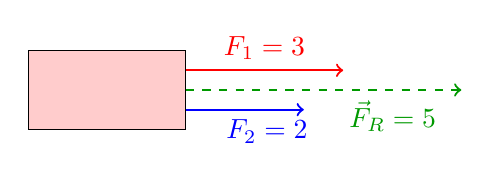
\begin{tikzpicture}
            % Block
            \draw[fill=red!20] (0,0) rectangle (2,1);

            % Force 1 (to the right)
            \draw[->, thick, red] (2,0.75) -- +(2,0) node[midway, above] {$F_1 = \qty{3}{\newton}$};

            % Force 2 (to the right)
            \draw[->, thick, blue] (2,0.25) -- +(1.5,0) node[midway, below,xshift=8] {$F_2 = \qty{2}{\newton}$};

            % Resultant force (to the right)
            \draw[->, thick, dashed, green!60!black] (2,0.5) -- +(3.5,0)
            node[midway, below, xshift=25] {$\vec{F}_R = \qty{5}{\newton}$};
        \end{tikzpicture}
        \caption{Fuerzas con el mismo sentido.}
    \end{figure}
    En este caso, la fuerza resultante \( F_R \), que es la suma de \( F_1 \) y \( F_2 \), será:
    \( \Sigma F_R = F_1 + F_2 = \qty{3}{\newton} + \qty{2}{\newton} = \qty{5}{\newton} \).

    \item \textbf{Fuerzas con sentido opuesto}.
    Ahora una de las fuerzas tendrá signo negativo; en el siguiente ejemplo será \( F_2 \).
    \begin{figure}[H]
        \centering
        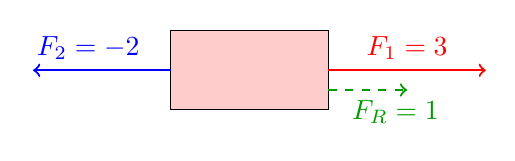
\begin{tikzpicture}
            % Block
            \draw[fill=red!20] (0,0) rectangle (2,1);

            % Force 1 (to the right)
            \draw[->, thick, red] (2,0.5) -- +(2,0) node[midway, above] {$F_1 = \qty{3}{\newton}$};

            % Force 2 (to the left)
            \draw[->, thick, blue] (0,0.5) -- +(-1.75,0) node[midway, above, xshift=-5] {$F_2= \qty{-2}{\newton}$};

            % Resultant force (to the right)
            \draw[->, thick, dashed, green!60!black] (2,0.25) -- +(1,0)
            node[midway, below, xshift=10] {$F_R = \qty{1}{\newton}$};
        \end{tikzpicture}
        \caption{Dos fuerzas con sentido opuesto.}
    \end{figure}
    En este caso, tenemos:
    \( \Sigma F_R = F_1 + F_2 = \qty{3}{\newton} - \qty{2}{\newton} = \qty{1}{\newton} \).
    Como \( F_2 \) va en dirección contraria, le asignamos el signo negativo.

    \item \textbf{Dos fuerzas perpendiculares}.
    Para obtener la fuerza resultante, debemos aplicar el teorema de Pitágoras.
    \begin{figure}[H]
        \centering
        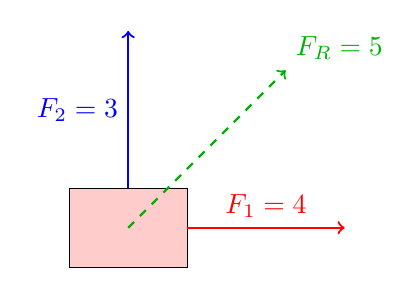
\begin{tikzpicture}
            % Block
            \draw[fill=red!20] (0,0) rectangle (1.5,1);

            % Force F1 (horizontal, right)
            \draw[->, thick, red] (1.5,0.5) -- +(2,0)
            node[midway, above] {$F_1 = \qty{4}{\newton}$};

            % Force F2 (vertical, upward)
            \draw[->, thick, blue] (0.75,1) -- +(0,2)
            node[midway, left] {$F_2 = \qty{3}{\newton}$};

            % Resultant vector
            \draw[->, thick, green!70!black, dashed] (0.75,0.5) -- +(2,2)
            node[above right] {$F_R = \qty{5}{\newton}$};
        \end{tikzpicture}
        \caption{Dos fuerzas perpendiculares.}
        \label{fig:two_perpendicular_forces}
    \end{figure}
    En este caso:
    \( F_R^2 = F_1^2 + F_2^2 \;\;\longrightarrow\;\; F_R = \sqrt{F_1^2 + F_2^2} \).

    \( F_R = \sqrt{3^2 + 4^2} = \qty{5}{\newton} \).
\end{itemize}


\begin{exercise}
    Dos caballos tiran de un carro en la misma dirección con una fuerza de 300 N cada uno.
    Calcula la magnitud y la dirección de la fuerza resultante.


    \begin{solu}
        Como ambos caballos tiran en la misma dirección, las fuerzas son paralelas y del mismo sentido, así que simplemente sumamos sus magnitudes.

        \textbf{Datos:}
        \begin{itemize}
            \item $F_1 = 300$ N
            \item $F_2 = 300$ N
            \item Ambas fuerzas en la misma dirección
        \end{itemize}

        \textbf{Solución:}

        La fuerza resultante es:
        $$F_R = F_1 + F_2 = 300\text{ N} + 300\text{ N} = 600\text{ N}$$

        \textbf{Respuesta:} La magnitud de la fuerza resultante es 600 N, y su dirección es la misma que la dirección en la que tiran ambos caballos (hacia delante).
    \end{solu}
\end{exercise}


\begin{exercise}
    Dibuja las fuerzas que se muestran a continuación, aplicadas en el origen de los ejes X e Y:
    \begin{enumerate}[label=\letraminuscula]
        \item una fuerza de magnitud 6 N, hacia abajo.
        \item una fuerza igual a la del apartado a., pero en la dirección opuesta.
        \item una fuerza de magnitud 7 N, en dirección horizontal y hacia la izquierda.
        \item una fuerza de magnitud 4 N cuya dirección forma un ángulo de 45° con el eje X positivo.
    \end{enumerate}


    \begin{solu}
        Los estudiantes deben dibujar un sistema de coordenadas con el origen en el centro, y luego dibujar cuatro vectores de fuerza:

        \textbf{a)} Dibuja una flecha apuntando hacia abajo a lo largo del eje Y negativo con magnitud 6 N. Etiquétala como $\vec{F}_1 = 6$ N hacia abajo.

        \textbf{b)} Dibuja una flecha apuntando hacia arriba a lo largo del eje Y positivo con magnitud 6 N. Etiquétala como $\vec{F}_2 = 6$ N hacia arriba.

        \textbf{c)} Dibuja una flecha apuntando hacia la izquierda a lo largo del eje X negativo con magnitud 7 N. Etiquétala como $\vec{F}_3 = 7$ N hacia la izquierda.

        \textbf{d)} Dibuja una flecha con un ángulo de 45° respecto al eje X positivo (apuntando hacia el primer cuadrante) con magnitud 4 N. Este vector debe formar ángulos iguales con ambos ejes. Etiquétala como $\vec{F}_4 = 4$ N a 45°.

        Todos los vectores deben originarse en el origen y dibujarse a escala.
    \end{solu}
\end{exercise}


\begin{exercise}
    Dos compañeros empujan una mesa en la misma dirección con fuerzas de 110 N y 135 N. Halla la fuerza resultante con la que empujan la mesa.
    Dibuja el diagrama de fuerzas.


    \begin{solu}
        Como ambos compañeros empujan en la misma dirección, sumamos las fuerzas algebraicamente.

        \textbf{Datos:}
        \begin{itemize}
            \item $F_1 = 110$ N
            \item $F_2 = 135$ N
            \item Ambas fuerzas en la misma dirección
        \end{itemize}

        \textbf{Solución:}
        $$F_R = F_1 + F_2 = 110\text{ N} + 135\text{ N} = 245\text{ N}$$

        \textbf{Diagrama de fuerzas:} Dibuja dos flechas apuntando en la misma dirección (por ejemplo, hacia la derecha) etiquetadas 110 N y 135 N. Luego dibuja una flecha más larga en la misma dirección etiquetada 245 N que representa la fuerza resultante.

        \textbf{Respuesta:} La fuerza resultante es 245 N en la dirección en la que ambos empujan.
    \end{solu}
\end{exercise}


\begin{exercise}
    Estos dos perros tiran de cada extremo de un juguete de goma.
    El perro de la derecha tira con una fuerza de magnitud 80 N y el de la izquierda con una fuerza de 95 N.
    \begin{enumerate}[label=\letraminuscula]
        \item Halla la magnitud y la dirección de la fuerza resultante.
        \item Dibuja un diagrama de fuerzas de las dos fuerzas y
        de la fuerza resultante.
    \end{enumerate}


    \begin{solu}
        \textbf{a) Magnitud y dirección de la fuerza resultante:}

        Como los perros tiran en direcciones opuestas, restamos las fuerzas. Tomando la dirección derecha como positiva:

        \textbf{Datos:}
        \begin{itemize}
            \item $F_{right} = 80$ N (hacia la derecha)
            \item $F_{left} = 95$ N (hacia la izquierda)
        \end{itemize}

        $$F_R = F_{right} - F_{left} = 80\text{ N} - 95\text{ N} = -15\text{ N}$$

        El signo negativo indica que la dirección es hacia la izquierda.

        \textbf{Respuesta:} La magnitud de la fuerza resultante es 15 N, dirigida hacia la izquierda (en la dirección del perro que tira con más fuerza).

        \textbf{b) Diagrama de fuerzas:} Dibuja dos flechas apuntando en direcciones opuestas: una hacia la derecha etiquetada 80 N y otra hacia la izquierda etiquetada 95 N. Luego dibuja una flecha más corta hacia la izquierda etiquetada 15 N que representa la fuerza resultante.
    \end{solu}
\end{exercise}




\begin{exercise}
    El resultado de dos fuerzas perpendiculares aplicadas a un cuerpo es 25 N.
    Si una de las fuerzas tiene una magnitud de 7 N, halla la magnitud de la otra fuerza.


    \begin{solu}
        Usamos el teorema de Pitágoras ya que las fuerzas son perpendiculares.

        \textbf{Datos:}
        \begin{itemize}
            \item $F_R = 25$ N (fuerza resultante)
            \item $F_1 = 7$ N (una de las fuerzas)
            \item $F_2 = ?$ (fuerza desconocida)
            \item Las fuerzas son perpendiculares
        \end{itemize}

        \textbf{Solución:}

        Del teorema de Pitágoras:
        $$F_R^2 = F_1^2 + F_2^2$$

        Despejando $F_2$:
        $$F_2 = \sqrt{F_R^2 - F_1^2} = \sqrt{(25)^2 - (7)^2} = \sqrt{625 - 49} = \sqrt{576} = 24\text{ N}$$

        \textbf{Respuesta:} La magnitud de la otra fuerza es 24 N.
    \end{solu}
\end{exercise}



\begin{exercise}
    Dos grupos de estudiantes tiran de un objeto, con la misma fuerza de 250 N, usando cuerdas atadas a lados opuestos del objeto.
    \begin{enumerate}[label=\letraminuscula]
        \item ¿Cuál es la fuerza resultante?
        \item Si el grupo de la derecha ahora tira con una fuerza de 325 N, calcula la fuerza resultante y su dirección.
    \end{enumerate}

    \begin{solu}
        \textbf{a) Fuerza resultante cuando ambos grupos tiran con 250 N:}

        Como los grupos tiran en direcciones opuestas con igual magnitud, las fuerzas se cancelan entre sí.

        Tomando la dirección derecha como positiva:
        $$F_R = F_{right} - F_{left} = 250\text{ N} - 250\text{ N} = 0\text{ N}$$

        \textbf{Respuesta:} La fuerza resultante es 0 N. El objeto permanece en equilibrio.

        \textbf{b) Fuerza resultante cuando el grupo de la derecha tira con 325 N:}

        Ahora las fuerzas son desiguales:
        $$F_R = F_{right} - F_{left} = 325\text{ N} - 250\text{ N} = 75\text{ N}$$

        \textbf{Respuesta:} La fuerza resultante es 75 N dirigida hacia la derecha (en la dirección de la fuerza más fuerte).
    \end{solu}
\end{exercise}





\begin{exercise}
    Dos fuerzas independientes, cada una de 100 N, actúan sobre el mismo objeto formando un ángulo de \ang{90}.
    Halla la magnitud de la fuerza resultante y dibuja su dirección en un diagrama de fuerzas.

    \begin{solu}
        Cuando dos fuerzas son perpendiculares entre sí, usamos el teorema de Pitágoras para hallar la magnitud de la fuerza resultante.

        \textbf{Datos:}
        \begin{itemize}
            \item $F_1 = 100$ N
            \item $F_2 = 100$ N
            \item Ángulo entre las fuerzas = 90°
        \end{itemize}

        \textbf{Solución:}

        Usando el teorema de Pitágoras:
        $$F_R = \sqrt{F_1^2 + F_2^2} = \sqrt{(100)^2 + (100)^2} = \sqrt{10000 + 10000} = \sqrt{20000} = 141.42\text{ N}$$

        La dirección de la fuerza resultante forma un ángulo de 45° con cada una de las fuerzas originales (ya que son iguales y perpendiculares).

        \textbf{Diagrama de fuerzas:} Dibuja dos flechas perpendiculares de igual longitud (100 N cada una), una horizontal y otra vertical. Luego dibuja la resultante como la diagonal del rectángulo formado, etiquetada 141.42 N, a 45° de cada fuerza original.

        \textbf{Respuesta:} La magnitud de la fuerza resultante es aproximadamente 141.42 N, dirigida a 45° de cada fuerza original.
    \end{solu}
\end{exercise}


\section{Deformación de los cuerpos}


Hemos visto anteriormente que una fuerza puede producir una deformación.
Podemos distinguir principalmente dos tipos de deformación:

\begin{itemize}
    \item \textbf{Deformación plástica}: se produce cuando el cuerpo deformado no recupera su forma original después de que cesa la fuerza.
    Es un proceso irreversible y permanente.
    \item \textbf{Deformación elástica}: es la deformación que desaparece cuando cesa la fuerza externa que la produjo.
    En esta unidad, estudiaremos este tipo de deformación.
\end{itemize}

\subsection{Fuerza elástica: Ley de Hooke}

Este tipo de fuerza se refiere a las fuerzas que surgen cuando deformamos un material elástico.

Así, bajo la acción de una fuerza, un muelle puede experimentar alargamiento o compresión hasta que la fuerza desaparece.

\begin{dBox}
    \textbf{Ley de Hooke}: la deformación de un muelle elástico es proporcional a la fuerza deformadora.
    La fuerza elástica que calculemos en un muelle dado será igual en magnitud y dirección, pero de sentido opuesto a la fuerza que causa dicha deformación (más adelante veremos que esto corresponde a la 3ª ley de Newton).
\end{dBox}

\begin{remark}
    La fuerza elástica siempre tendrá signo negativo porque se opone a la dirección de la fuerza aplicada.
    Aquí no incluiremos el signo porque solo estamos determinando la magnitud, no la dirección.
\end{remark}

\vspace*{20pt}
\begin{centeredequation}
    \eqnmarkbox[blue]{elasticforce}{F_{\text{elastic}}}
    =
    \eqnmarkbox[red]{springconstant}{k}
    \cdot
    \eqnmarkbox[mygreen]{elongation}{\Delta l}
\end{centeredequation}
\annotate[yshift=1em]{left}{elasticforce}{Fuerza elástica}
\annotate[yshift=1em]{}{springconstant}{Constante elástica propia de cada muelle}
\annotate[yshift=-2em]{below,left}{elongation}{Longitud que se ha estirado o comprimido el muelle}
\vspace*{12pt}

Para calcular \( \Delta l \), podemos usar la expresión: \( \Delta l = l_f - l_i \), donde \( l_f \) es la longitud final del muelle y \( l_i \) es la longitud inicial del muelle.

\begin{remark}
    Si nos dicen que un muelle se ha estirado o comprimido una determinada distancia, esto nos da directamente el valor de \( \Delta l \).
\end{remark}

Cada muelle tiene su propia constante elástica, cuyas unidades en el Sistema Internacional son \unit{\newton\per\metre}.

\subsection{Medida de fuerzas}

\begin{minipage}{0.6\textwidth}
    Para medir fuerzas, se utiliza un \textbf{dinamómetro}.

    Un dinamómetro es un instrumento con un muelle que tiene una constante elástica conocida.
    Este muelle tiene una escala acoplada calibrada en newtons, que nos permite medir fuerzas.
    Para calcular estas fuerzas, usamos la ley de Hooke estudiada anteriormente.

    Su uso es básico: si queremos calcular la fuerza ejercida por un objeto (normalmente su peso), colgamos el objeto del gancho del dinamómetro.
\end{minipage}
\hfill
\begin{minipage}{0.35\textwidth}
    \begin{figure}[H]
        \centering
%        \includegraphics[scale=0.20]{images/dinamica/dinanometro}
        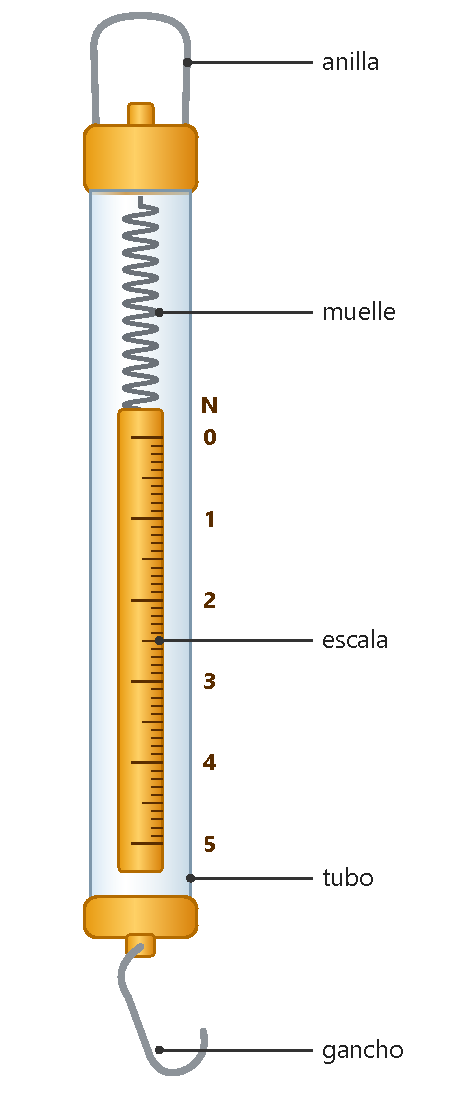
\includegraphics[width=0.6\linewidth]{Figuras_SVG_ES/pdf/U3_dinamometro.pdf}
        \caption{Dinamómetro}
        \label{fig:dinamometro}
    \end{figure}
    \vspace{6pt}
\end{minipage}

Dijimos anteriormente que la fuerza ejercida por un objeto es igual a la fuerza elástica, por lo que podemos aplicar:
\begin{centeredequation}
    F_{\text{elastic}} = F_{\text{object}}
\end{centeredequation}

Como conocemos la constante elástica del dinamómetro y medimos el alargamiento del muelle, podemos calcular fácilmente la fuerza del objeto usando:
\begin{centeredequation}
    F_{\text{object}} = k \cdot \Delta l
\end{centeredequation}

\begin{exercise}
    Cuando se aplica una fuerza de 20 N a un determinado muelle, este produce un alargamiento de 10 cm.
    \begin{enumerate}[label=\alph*)]
        \item Calcula la constante elástica.
        \item Calcula el alargamiento del muelle cuando se aplica una fuerza de 200 N.
        \item Determina la fuerza necesaria para producir un alargamiento de 5 dm.
    \end{enumerate}

    \begin{solu}
        Usamos la Ley de Hooke: $F = k \cdot \Delta x$

        \textbf{Datos:}
        \begin{itemize}
            \item $F = 20$ N
            \item $\Delta x = 10$ cm = 0.10 m
        \end{itemize}

        \textbf{a) Calcular la constante elástica:}

        De la Ley de Hooke:
        $$k = \frac{F}{\Delta x} = \frac{20\text{ N}}{0.10\text{ m}} = 200\text{ N/m}$$

        \textbf{Respuesta:} La constante elástica es 200 N/m.

        \textbf{b) Alargamiento cuando F = 200 N:}

        $$\Delta x = \frac{F}{k} = \frac{200\text{ N}}{200\text{ N/m}} = 1\text{ m} = 100\text{ cm}$$

        \textbf{Respuesta:} El alargamiento es 1 m o 100 cm.

        \textbf{c) Fuerza necesaria para un alargamiento de 5 dm:}

        Primero, convertimos: 5 dm = 0.5 m

        $$F = k \cdot \Delta x = 200\text{ N/m} \times 0.5\text{ m} = 100\text{ N}$$

        \textbf{Respuesta:} Se necesita una fuerza de 100 N.
    \end{solu}
\end{exercise}

\begin{exercise}
    En un experimento para determinar la constante elástica, se obtuvieron los siguientes resultados:
    \begin{table}[H]
        \centering
        \renewcommand{\arraystretch}{1.5}
        \begin{tabular}{Occccc}
            \bottomrule
            \textcolor{ocre}{\textbf{F (\unit{\newton})}}      & 0 & 5   & 10 & 15 & 20  \\
            \hline
            \textcolor{ocre}{\textbf{x (\unit{\centi\metre})}} & 0 & 2.1 & 4  & 6  & 7.9 \\
            \toprule
        \end{tabular}
        \label{tab:ejercicio1}
    \end{table}
%    \begin{figure}[H]
%        \centering
%        \includegraphics{images/dinamica/ejercicio_9}
%    \end{figure}
    \begin{enumerate}[label=\alph*)]
        \item Representa los datos de la tabla en una gráfica.
        \item ¿Cuál es el valor de la constante elástica?
    \end{enumerate}

    \begin{solu}
        \textbf{Nota:} Dado que la imagen con la tabla de datos no está disponible en el texto, se ofrece un método general de resolución.

        \textbf{a) Representación de los datos:}

        Los estudiantes deben crear una gráfica con:
        \begin{itemize}
            \item Eje X: Extensión/Alargamiento ($\Delta x$) en metros
            \item Eje Y: Fuerza (F) en Newtons
            \item Representar todos los puntos de datos de la tabla
            \item Trazar una línea recta de mejor ajuste que pase por el origen
        \end{itemize}

        \textbf{b) Cálculo de la constante elástica:}

        Según la Ley de Hooke: $F = k \cdot \Delta x$

        Esta es una relación lineal de la forma $y = mx$ donde:
        \begin{itemize}
            \item La pendiente ($m$) es igual a la constante elástica ($k$)
            \item $k = \frac{F}{\Delta x}$ o $k = \frac{\Delta F}{\Delta \Delta x}$
        \end{itemize}

        Para hallar $k$:
        \begin{enumerate}
            \item Elige dos puntos de la línea: $(x_1, y_1)$ y $(x_2, y_2)$
            \item Calcula la pendiente: $k = \frac{y_2 - y_1}{x_2 - x_1} = \frac{F_2 - F_1}{\Delta x_2 - \Delta x_1}$
        \end{enumerate}

        \textbf{Respuesta:} La constante elástica es la pendiente de la gráfica Fuerza vs. Extensión, medida en N/m.
    \end{solu}
\end{exercise}

\begin{exercise}
    Halla la fuerza necesaria para estirar un muelle con una constante de 150 N/m en 3 cm desde su longitud inicial.

    \begin{solu}
        Usamos la Ley de Hooke: $F = k \cdot \Delta x$

        \textbf{Datos:}
        \begin{itemize}
            \item $k = 150$ N/m
            \item $\Delta x = 3$ cm = 0.03 m
        \end{itemize}

        \textbf{Solución:}
        $$F = k \cdot \Delta x = 150\text{ N/m} \times 0.03\text{ m} = 4.5\text{ N}$$

        \textbf{Respuesta:} Se necesita una fuerza de 4.5 N para estirar el muelle 3 cm.
    \end{solu}
\end{exercise}


\section{Leyes de Newton}

\subsection{Primera ley de Newton: Ley de la inercia}

Conocida como la \textbf{Ley de la inercia}, establece lo siguiente:
\begin{dBox}
    \textbf{Primera ley de Newton: Ley de la inercia}. Todo cuerpo permanece en reposo o en movimiento rectilíneo uniforme a menos que actúe sobre él una fuerza externa.
\end{dBox}

\subsection{Segunda ley de Newton: Principio fundamental de la dinámica}

\begin{dBox}
    \textbf{Segunda ley de Newton: Principio fundamental de la dinámica}. La aceleración de un cuerpo es directamente proporcional a la fuerza aplicada sobre dicho cuerpo. Además, el cambio de velocidad del cuerpo se produce a lo largo de la línea de acción de la fuerza aplicada.
    \begin{centeredequation}
        \Sigma F = m\ a
    \end{centeredequation}
\end{dBox}

\begin{exercise}
    Se aplica una fuerza de 5 N a un cuerpo de masa 0.2 kg.
    ¿Qué aceleración adquirirá el cuerpo?

    \begin{solu}
        Usamos la Segunda ley de Newton: $F = m \cdot a$
        \textbf{Datos:}
        \begin{itemize}
            \item $F = 5$ N
            \item $m = 0.2$ kg
        \end{itemize}

        \textbf{Solución:}

        Despejando la aceleración:
        $$a = \frac{F}{m} = \frac{5\text{ N}}{0.2\text{ kg}} = 25\text{ m/s}^2$$

        \textbf{Respuesta:} El cuerpo adquirirá una aceleración de 25 m/s².
    \end{solu}
\end{exercise}

\begin{exercise}
    Un hombre de 75 kg de masa está sentado en un coche que empieza a moverse con una aceleración de 1.5 m/s².
    ¿Qué fuerza experimenta el hombre?

    \begin{solu}
        Usamos la Segunda ley de Newton: $F = m \cdot a$

        \textbf{Datos:}
        \begin{itemize}
            \item $m = 75$ kg
            \item $a = 1.5$ m/s²
        \end{itemize}

        \textbf{Solución:}
        $$F = m \cdot a = 75\text{ kg} \times 1.5\text{ m/s}^2 = 112.5\text{ N}$$

        \textbf{Respuesta:} El hombre experimenta una fuerza de 112.5 N en la dirección de la aceleración del coche. Esta fuerza la ejerce el asiento empujándolo hacia delante.
    \end{solu}
\end{exercise}

\begin{exercise}
    Calcula la fuerza horizontal que se aplica a un cuerpo de masa 25 kg que se mueve a una velocidad constante de 25 km/h sobre una superficie horizontal.

    \begin{solu}
        Según la Primera ley de Newton, si un cuerpo se mueve a velocidad constante, la fuerza neta que actúa sobre él es cero.

        \textbf{Datos:}
        \begin{itemize}
            \item $m = 25$ kg
            \item $v = 25$ km/h = constante
        \end{itemize}

        \textbf{Solución:}

        Si la velocidad es constante, la aceleración es cero:
        $$a = 0\text{ m/s}^2$$

        Usando la Segunda ley de Newton:
        $$F_{net} = m \cdot a = 25\text{ kg} \times 0\text{ m/s}^2 = 0\text{ N}$$

        Esto significa que si hay rozamiento, la fuerza horizontal aplicada debe ser igual a la fuerza de rozamiento para mantener la velocidad constante. Sin embargo, si suponemos que no hay rozamiento (o la pregunta pide la fuerza neta), la respuesta es 0 N.

        \textbf{Respuesta:} La fuerza horizontal neta es 0 N, ya que el cuerpo se mueve a velocidad constante (sin aceleración). Si hay rozamiento, la fuerza aplicada es igual a la fuerza de rozamiento, pero la fuerza neta sigue siendo cero.
    \end{solu}
\end{exercise}

\begin{exercise}
    Calcula la fuerza que una persona debe aplicar a una mesa de masa 20 kg para darle una aceleración de \qty{1.25}{\mpss}.
    Si otra persona está en el lado opuesto de la mesa, ¿qué fuerza debe aplicar para evitar que se mueva?

    \begin{solu}
        Usamos la Segunda ley de Newton: $F = m \cdot a$

        \textbf{Datos:}
        \begin{itemize}
            \item $m = 20$ kg
            \item $a = 1.25$ m/s²
        \end{itemize}

        \textbf{Solución para la primera parte:}
        $$F = m \cdot a = 20\text{ kg} \times 1.25\text{ m/s}^2 = 25\text{ N}$$

        \textbf{Respuesta:} La persona debe aplicar una fuerza de 25 N.

        \textbf{Solución para la segunda parte:}

        Para evitar que la mesa se mueva, la persona del lado opuesto debe aplicar una fuerza igual en la dirección opuesta para crear equilibrio (fuerza neta = 0).

        \textbf{Respuesta:} La persona del lado opuesto debe aplicar una fuerza de 25 N en la dirección opuesta para evitar que la mesa se mueva.
    \end{solu}
\end{exercise}

\begin{exercise}
    Dos chicas están empujando un armario de madera de 50 kg sobre un suelo horizontal.
    Cada una de ellas ejerce una fuerza de 25 N. Halla la aceleración del armario.
    ¿Cuál es su dirección respecto a las chicas?

    \begin{solu}
        Usamos la Segunda ley de Newton: $F = m \cdot a$

        \textbf{Datos:}
        \begin{itemize}
            \item $m = 50$ kg
            \item $F_1 = 25$ N
            \item $F_2 = 25$ N
            \item Suponiendo que ambas chicas empujan en la misma dirección
        \end{itemize}

        \textbf{Solución:}

        Primero, calculamos la fuerza total:
        $$F_{total} = F_1 + F_2 = 25\text{ N} + 25\text{ N} = 50\text{ N}$$

        Luego, aplicamos la Segunda ley de Newton:
        $$a = \frac{F_{total}}{m} = \frac{50\text{ N}}{50\text{ kg}} = 1\text{ m/s}^2$$

        \textbf{Respuesta:} La aceleración del armario es 1 m/s². La dirección es la misma que la dirección en la que empujan ambas chicas (suponiendo que empujan en la misma dirección).
    \end{solu}
\end{exercise}

\subsection{Tercera ley de Newton: Ley de acción y reacción}

\begin{dBox}
    \textbf{Tercera ley de Newton: Ley de acción y reacción}: Cuando dos cuerpos interactúan, ejercen fuerzas mutuas que son iguales en magnitud pero opuestas en dirección.
\end{dBox}

Si denotamos la fuerza que el objeto A ejerce sobre el objeto B como (\( F_{AB} \)) y la fuerza que el objeto B ejerce sobre el objeto A como (\( F_{BA} \)), tenemos:
\begin{centeredequation}
    F_{AB} = - F_{BA}
\end{centeredequation}


\section{Fuerza gravitatoria}

Es una de las cuatro fuerzas fundamentales y es responsable de la estructura del universo.
Es una interacción que se produce entre dos cuerpos con masa, es \textbf{siempre atractiva} y tiene alcance ilimitado.

En el siglo XVII, Isaac Newton consideró que la fuerza que la Tierra ejerce sobre la Luna es la misma que se ejerce sobre cualquier cuerpo en la superficie de la Tierra: la atracción gravitatoria.
Extendió esta interacción a todos los planetas, afirmando que la gravedad es un atributo de todos los cuerpos y es proporcional a la cantidad de materia que contiene cada uno.

La intensidad de la fuerza gravitatoria depende de las masas de los cuerpos y de la distancia entre ellos.
Así, cuanto mayor sea la masa de un cuerpo, mayor será la fuerza gravitatoria que produce.
Sin embargo, cuanto mayor sea la distancia entre los cuerpos, menor será la fuerza gravitatoria.
La fuerza gravitatoria se suele representar por \( F_G \) y se expresa como:

\begin{centeredequation}
    F_G = G \cdot \dfrac{m_1 \cdot m_2}{r^2}
\end{centeredequation}

Donde \( G \) es la constante de gravitación universal con un valor de \( G = \qty{6.67e-11}{\newton\square\metre\per\square\kilo\g} \), \( m_1 \) y \( m_2 \) son las masas de los dos cuerpos, y \( r \) es la distancia entre ellos.
Como la fuerza gravitatoria es una fuerza, se mide en Newtons.

\begin{remark}
    La distancia entre los dos objetos se mide siempre desde el centro de cada objeto.
\end{remark}

\begin{remark}
    Para los planetas, mide la distancia desde el centro de cada planeta, y como son grandes, debes conocer el radio de cada planeta.
\end{remark}

Si queremos calcular la fuerza gravitatoria que la Tierra ejerce sobre un objeto en su superficie con masa \( m \), aplicamos la siguiente ecuación:
\vspace*{31pt}
\begin{centeredequation}
    \eqnmarkbox[red]{gravitationalforce}{F_G}
    =
    G \cdot
    \dfrac{\eqnmarkbox[blue]{earthmass}{M_T} \cdot m}{\eqnmarkbox[mygreen]{earthradius}{R_T^2}}
\end{centeredequation}

\annotate[yshift=1em]{left}{gravitationalforce}{Fuerza que ejerce la Tierra sobre el objeto}
\annotate[yshift=1em]{}{earthmass}{Masa de la Tierra}
\annotate[yshift=-2em]{below,left}{earthradius}{Radio de la Tierra}
\vspace*{31pt}

Si queremos calcular la fuerza que la Tierra ejerce sobre un objeto a una altura \( h \) sobre la superficie terrestre, debemos sumar esa altura \( h \) al radio de la Tierra, obteniendo:
\begin{centeredequation}
    F_G = G \cdot \dfrac{M_T \cdot m}{(R_T + h)^2}
\end{centeredequation}

\begin{remark}
    Recuerda convertir todas las magnitudes a unidades del SI antes de usarlas en las fórmulas.
\end{remark}

\subsection{Gravedad o campo gravitatorio}
\begin{definition}[Gravedad o campo gravitatorio]
Es la atracción generada en el espacio por una masa a su alrededor.
\end{definition}

Por ejemplo, la Tierra tiene un campo gravitatorio en su superficie de \qty{9.8}{\mpss}, pero este valor disminuye a medida que ascendemos.
Como podemos ver, la gravedad tiene las mismas unidades que la aceleración, \unit{\mpss}
La expresión para la gravedad es:

\begin{centeredequation}
    g = G \cdot \dfrac{m}{r^2}
\end{centeredequation}

Donde \( m \) es la masa del cuerpo que ejerce la fuerza gravitatoria y \( r \) es la distancia entre el centro de dicho cuerpo y el punto donde queremos calcular la gravedad.

La fórmula para calcular la gravedad en la superficie terrestre es:

\begin{centeredequation}
    g_T = G \cdot \dfrac{M_T}{R_T^2}
\end{centeredequation}

Para calcular la gravedad a una altura \( h \) sobre la superficie terrestre, la expresión es:

\begin{centeredequation}
    g_T = G \cdot \dfrac{M_T}{(R_T+h)^2}
\end{centeredequation}

\begin{remark}
    La gravedad en la superficie de los planetas es diferente, por lo que para calcularla debemos conocer la masa y el radio del planeta.
\end{remark}

\newpage

\begin{centeredequation}
    g_{\text{Planet}} = G \cdot \dfrac{M_{\text{Planet}}}{R_{\text{Planet}}^2}
\end{centeredequation}

\begin{remark}
    Recuerda convertir todas las magnitudes a unidades del SI antes de usarlas en las fórmulas.
\end{remark}

\subsection{Fuerza peso (p o w)}

De hecho, la fuerza gravitatoria se llama \textbf{Peso}.

\begin{definition}[Fuerza peso]
    Es la fuerza con la que la Tierra, o cualquier otro planeta, atrae a los cuerpos que están en él.
    Dada la masa de cualquier persona u objeto en la Tierra o en otro planeta, el peso de dicho objeto o persona viene dado por:
    \begin{centeredequation}
        w = m \cdot g \quad \text{o} \quad p = m \cdot g
    \end{centeredequation}
    Donde \( m \) es la masa del objeto y \( g \) es la gravedad de dicho planeta.
\end{definition}

Como el peso es una fuerza, su unidad es el Newton.

Como podemos ver en la fórmula del peso, esta fuerza depende de la masa de cada objeto, así como de la gravedad del planeta en el que nos encontremos.

\begin{remark}
    La gravedad en la Luna es diferente de la de la Tierra; por lo tanto, para calcular el peso en la Luna, primero debemos calcular la gravedad en la Luna.
\end{remark}

\begin{exercise}
    Los satélites Meteosat de la Agencia Espacial Europea tienen una masa de 2000 kg y orbitan la Tierra en una trayectoria circular con un radio de 36000 km.
    Calcula la fuerza con la que la Tierra atrae a estos satélites.
    ¿Cuál es el efecto de esta fuerza sobre los satélites?

    \datos{} \Ggravitacion; \( M_T = \qty{5.99e24}{\kilo\g} \); \( R_T = \qty{6380}{\kilo\metre} \)

    \begin{solu}
        Usamos la Ley de Gravitación Universal de Newton: $F = \frac{G \cdot M_1 \cdot M_2}{r^2}$

        \textbf{Datos:}
        \begin{itemize}
            \item $G = 6.67 \times 10^{-11}$ N·m²/kg²
            \item $M_{Earth} = 5.99 \times 10^{24}$ kg
            \item $m_{satellite} = 2000$ kg
            \item $r = 36000$ km = $3.6 \times 10^7$ m (radio orbital desde el centro de la Tierra)
        \end{itemize}

        \textbf{Solución}
    \end{solu}
\end{exercise}



\begin{exercise}
    En un determinado planeta, medimos el peso de una masa de 9 kg con un dinamómetro y obtenemos una lectura de 108 N. ¿Cuál es el valor de \( g \) en ese planeta?
    \begin{solu}
        Usamos la relación entre peso y masa: $W = m \cdot g$

        \textbf{Datos:}
        \begin{itemize}
            \item $m = 9$ kg
            \item $W = 108$ N
        \end{itemize}

        \textbf{Solución:}

        Despejando $g$:
        $$g = \frac{W}{m} = \frac{108\text{ N}}{9\text{ kg}} = 12\text{ m/s}^2$$

        \textbf{Respuesta:} El valor de $g$ en ese planeta es 12 m/s².
    \end{solu}
\end{exercise}

\begin{exercise}
    A partir de observaciones astronómicas, sabemos que Júpiter tiene un radio de \qty{6.98e7}{\metre} y una masa de \qty{1.9e27}{\kilo\g}.
    Calcula la aceleración de la gravedad en este planeta.

    \datos{}: \Ggravitacion

    \begin{solu}
        Usamos la fórmula de la aceleración gravitatoria: $g = \frac{G \cdot M}{R^2}$

        \textbf{Datos:}
        \begin{itemize}
            \item $G = 6.67 \times 10^{-11}$ N·m²/kg²
            \item $M_{Jupiter} = 1.9 \times 10^{27}$ kg
            \item $R_{Jupiter} = 6.98 \times 10^{7}$ m
        \end{itemize}

        \textbf{Solución:}
        $$g_{Jupiter} = \frac{G \cdot M_{Jupiter}}{R_{Jupiter}^2} = \frac{6.67 \times 10^{-11} \times 1.9 \times 10^{27}}{(6.98 \times 10^7)^2}$$

        $$g_{Jupiter} = \frac{1.267 \times 10^{17}}{4.872 \times 10^{15}} = 26.0\text{ m/s}^2$$

        \textbf{Respuesta:} La aceleración de la gravedad en Júpiter es aproximadamente 26.0 m/s², lo que equivale a unas 2.65 veces la gravedad terrestre.
    \end{solu}
\end{exercise}



\begin{exercise}
    Colgamos una masa de 500 g de un dinamómetro, y su escala marca 4.85 N. ¿Cuál es el valor de \( g \)?
\end{exercise}

\begin{exercise}
    Medimos la masa de un objeto usando una balanza de laboratorio y obtenemos 0.9 kg.
    Trabaja con un compañero para calcular su peso.
\end{exercise}


\begin{exercise}
    Un chico pesa 441 N en la Tierra.
    En tu cuaderno, responde a las siguientes preguntas:
    \begin{enumerate}[label=\alph*)]
\item ¿Cuál es el peso del chico en Marte?
\item ¿Cuál es su masa en la Luna?
\item ¿Cuál es su peso en la Luna?
    \end{enumerate}

    \datos{}: \( g_{\text{Mars}} = \qty{3.7}{\mpss} \); \( g_{\text{Moon}} = \qty{1.6}{\mpss} \)
\end{exercise}


\begin{exercise}
    El monte Chimborazo es el punto más alejado del centro de gravedad de la Tierra, a 6268 m sobre el nivel del mar (lo que supone 6 378 000 metros desde el centro de masa de la Tierra).
    Halla \( g \) en la cima del Chimborazo y compárala con \( g \) al nivel del mar (\qty{9.8}{\mpss}).
\end{exercise}

\begin{exercise}
    El Hubble es un telescopio que permanece en órbita alrededor de la Tierra a una altitud de 600 km sobre su superficie.
    Determina la aceleración gravitatoria a la que está sometido el Hubble.

    \datos{}: \Ggravitacion; \( M_T = \qty{5.99e24}{\kilo\g} \); \( R_T = \qty{6380}{\kilo\metre} \)
\end{exercise}


\begin{exercise}
    Calcula el peso de una persona de 80 kg situada a la altura del monte Everest (8848 m).
    ¿Y a una altitud de 300 km?

    \datos{}: \Ggravitacion; \( M_T = \qty{5.99e24}{\kilo\g} \); \( R_T = \qty{6380}{\kilo\metre} \)
\end{exercise}


\begin{exercise}
    Calcula la gravedad en la Luna. ¿Qué fuerza ejerce la Luna sobre un astronauta de 95 kg de masa?

    \datos{}: \Ggravitacion; \( M_L = \qty{7.36e22}{\kilo\g} \); \( R_L = \qty{1740}{\kilo\metre} \)
\end{exercise}


\section{Fuerza eléctrica}

Como estudiamos anteriormente, el átomo está compuesto por dos partículas cargadas: los electrones, con carga negativa, y los protones, con carga eléctrica positiva.
Normalmente, los materiales tienen el mismo número de electrones que de protones y son neutros; sin embargo, debido a procesos de \textbf{electrización}, puede producirse una transferencia de electrones de un cuerpo a otro, creando un desequilibrio entre las cargas positivas y negativas en un cuerpo.

En este tipo de fuerza intervienen cargas eléctricas, y por ello debemos definir una nueva magnitud que nos permita cuantificar el valor de dicha carga (equivalente a la masa en la fuerza gravitatoria).
\begin{definition}[Carga eléctrica]
    Es una propiedad de la materia presente en las partículas subatómicas.
    La unidad de carga eléctrica es el Culombio, representado como \( \unit{\coulomb} \).

    Las cargas eléctricas pueden ser positivas o negativas.
\end{definition}

La fuerza eléctrica es otra de las cuatro fuerzas fundamentales de la naturaleza y se manifiesta cuando tenemos cargas eléctricas.
Las fuerzas eléctricas pueden ser \textbf{atractivas} cuando las cargas son de signo opuesto, y \textbf{repulsivas} cuando las cargas son del mismo signo.

En el siglo XVIII, Charles Coulomb descubrió las propiedades de esta fuerza y las relaciones entre las cargas y sus distancias, lo que dio lugar a la expresión:
\vspace{36pt}

\begin{centeredequation}
    \eqnmarkbox[red]{electricforce}{F_e} =
    \eqnmarkbox[mygreen]{coulombconstant}{K} \cdot
    \dfrac{\eqnmarkbox[blue]{charge1}{q_1} \cdot \eqnmarkbox[blue]{charge2}{q_2}}{\eqnmarkbox[myOrange]{chargedistance}{r^2}}
\end{centeredequation}

\annotate[yshift=1em]{left}{electricforce}{Fuerza eléctrica}
\annotate[yshift=1.25em]{}{coulombconstant}{Constante de Coulomb}
\annotate[yshift=-2em]{below,left}{charge1}{Carga de la partícula 1}
\annotate[yshift=-4em]{below,left}{charge2}{Carga de la partícula 2}
\annotate[yshift=-0.5em,xshift=1.5em]{below}{chargedistance}{Distancia entre las cargas}
\vspace{36pt}

\begin{remark}
    Para los cálculos, usa el valor absoluto de la carga, es decir, sin el signo.
\end{remark}

La constante de Coulomb (\( K \)) tiene un valor de \( K = \qty{9e9}{\newton\square\metre\per\square\coulomb} \).

\begin{remark}
    Es fundamental convertir todas las magnitudes a unidades del SI antes de sustituirlas en la fórmula, para evitar errores.
\end{remark}


\begin{exercise}
    Calcula la fuerza entre dos cargas:
    \begin{enumerate}[label=\alph*)]
\item \qty{+5}{\micro\coulomb} y \qty{+3}{\micro\coulomb} situadas a 10 cm de distancia.
\item \qty{+5}{\micro\coulomb} y \qty{-3}{\micro\coulomb} situadas a 10 cm de distancia.
    \end{enumerate}

    \datos{}: \ctecoulomb

\end{exercise}


\begin{exercise}
    ¿Cuál es la magnitud de la fuerza eléctrica ejercida sobre una carga de +7 C por otra carga de +3 C situada a 2 m de distancia?
    ¿Es la fuerza atractiva o repulsiva?

    \datos{}: \ctecoulomb

\end{exercise}

\begin{exercise}
    La masa de un protón es \qty{1.67e-27}{\kilo\g} y su carga eléctrica es \qty{1.6e-19}{\coulomb}.
    Compara la fuerza de repulsión eléctrica entre dos protones en el vacío a una distancia de 1 m con la atracción gravitatoria entre ellos.

    \datos{}: \ctecoulomb; \Ggravitacion

\end{exercise}


\begin{exercise}
    Elabora un mapa conceptual de la unidad.
    \begin{solu}
        Este es un ejercicio creativo en el que los estudiantes deben organizar los conceptos principales de la unidad de forma jerárquica o conectada. El mapa conceptual debe incluir:

        \textbf{Conceptos principales a incluir:}
        \begin{itemize}
            \item Fuerzas: definición, representación (magnitud, dirección, punto de aplicación)
            \item Tipos de fuerzas: fuerzas de contacto (rozamiento, normal, tensión) y fuerzas a distancia (gravitatoria, eléctrica)
            \item Suma vectorial de fuerzas
            \item Leyes del movimiento de Newton (Primera, Segunda y Tercera ley)
            \item Ley de Hooke y fuerzas elásticas
            \item Diferencia entre peso y masa
            \item Ley de Gravitación Universal
            \item Ley de Coulomb
        \end{itemize}
        Los estudiantes deben crear conexiones entre estos conceptos mostrando cómo se relacionan entre sí.
    \end{solu}
\end{exercise}


%\section{Vocabulario}
%
%\begin{vocabulary}[Force]
%A physical quantity that represents an interaction capable of changing the motion, speed, direction, or shape of an object. \newline
%\textbf{Translation to Spanish}: Fuerza \newline
%% Line 8
%\end{vocabulary}
%
%\begin{vocabulary}[Newton]
%The SI unit of force, defined as the force required to accelerate a mass of one kilogram at one meter per second squared. \newline
%\textbf{Translation to Spanish}: Newton \newline
%% Line 11
%\end{vocabulary}
%
%\begin{vocabulary}[Acceleration]
%The rate at which the velocity of an object changes with time. \newline
%\textbf{Translation to Spanish}: Aceleración \newline
%% Line 12
%\end{vocabulary}
%
%\begin{vocabulary}[Gravitational Force]
%The attractive force that exists between any two masses in the universe. \newline
%\textbf{Translation to Spanish}: Fuerza gravitatoria \newline
%% Line 16
%\end{vocabulary}
%
%\begin{vocabulary}[Electromagnetic Force]
%A fundamental force responsible for interactions between electrically charged particles. \newline
%\textbf{Translation to Spanish}: Fuerza electromagnética \newline
%% Line 17
%\end{vocabulary}
%
%\begin{vocabulary}[Strong Nuclear Force]
%The fundamental force that holds protons and neutrons together inside the nucleus of an atom. \newline
%\textbf{Translation to Spanish}: Fuerza nuclear fuerte \newline
%% Line 18
%\end{vocabulary}
%
%\begin{vocabulary}[Weak Nuclear Force]
%A fundamental force involved in radioactive decay and certain particle interactions. \newline
%\textbf{Translation to Spanish}: Fuerza nuclear débil \newline
%% Line 19
%\end{vocabulary}
%
%\begin{vocabulary}[Vector]
%A physical quantity that has both magnitude and direction. \newline
%\textbf{Translation to Spanish}: Vector \newline
%% Line 84
%\end{vocabulary}
%
%\begin{vocabulary}[Equilibrium]
%The state in which the net force acting on an object is zero, resulting in no acceleration. \newline
%\textbf{Translation to Spanish}: Equilibrio \newline
%% Line 337
%\end{vocabulary}
%
%\begin{vocabulary}[Weight]
%The gravitational force exerted on an object due to the presence of a massive body such as Earth. \newline
%\textbf{Translation to Spanish}: Peso \newline
%% Line 443
%\end{vocabulary}
%
%\begin{vocabulary}[Tension]
%A pulling force transmitted through a rope, cable, or string when it is stretched. \newline
%\textbf{Translation to Spanish}: Tensión \newline
%% Line 536
%\end{vocabulary}
%
%\begin{vocabulary}[Inertia]
%The tendency of an object to resist changes in its state of motion. \newline
%\textbf{Translation to Spanish}: Inercia \newline
%% Line 584
%\end{vocabulary}
%
%\begin{vocabulary}[Velocity]
%A vector quantity that describes the speed of an object together with its direction of motion. \newline
%\textbf{Translation to Spanish}: Velocidad \newline
%% Line 594
%\end{vocabulary}
%
%\begin{vocabulary}[Mass]
%A measure of the amount of matter contained in an object. \newline
%\textbf{Translation to Spanish}: Masa \newline
%% Line 601
%\end{vocabulary}
%
%\begin{vocabulary}[Newton's Second Law]
%A law stating that the acceleration of an object is proportional to the net force acting on it and inversely proportional to its mass. \newline
%\textbf{Translation to Spanish}: Segunda ley de Newton \newline
%% Line 605
%\end{vocabulary}
%
%\begin{vocabulary}[Net Force]
%The overall force acting on an object after all individual forces are combined vectorially. \newline
%\textbf{Translation to Spanish}: Fuerza neta \newline
%% Line 645
%\end{vocabulary}
%
%\begin{vocabulary}[Friction]
%A force that opposes the relative motion between two surfaces in contact. \newline
%\textbf{Translation to Spanish}: Fricción \newline
%% Line 661
%\end{vocabulary}
%
%\begin{vocabulary}[Gravity]
%The natural phenomenon by which masses attract each other. \newline
%\textbf{Translation to Spanish}: Gravedad \newline
%% Line 739
%\end{vocabulary}
%
%\begin{vocabulary}[Weight Force]
%The force exerted on an object due to gravity, usually directed toward the center of the Earth. \newline
%\textbf{Translation to Spanish}: Fuerza peso \newline
%% Line 827
%\end{vocabulary}
%
%\begin{vocabulary}[Electric Charge]
%A physical property of matter that causes it to experience a force in an electromagnetic field. \newline
%\textbf{Translation to Spanish}: Carga eléctrica \newline
%% Line 972
%\end{vocabulary}


%------------------------------------------------


    \chapterimage{Images/portada_cabeceras/cabecera_U4_energia}
    \chapter{Energía}

    %! Author = crist
%! Date = 03/12/2025

\spacing{1.3}


\section{Energía}
\begin{definition}[Energía]
    Se define como la capacidad de un cuerpo para producir cambios en sí mismo o en su entorno
\end{definition}
La unidad de energía en el Sistema Internacional es el Julio (\unit{\joule}). Otras formas de energía y su equivalencia en julios son:
\begin{itemize}
    \item \textbf{Caloría (\unit{\calorie})}. \( \qty{1}{\calorie} = \qty{4.18}{\joule} \).
    \item \textbf{Kilovatio-hora} (\unit{\kwh}) \( \longrightarrow \) \( \qty{1}{\kwh} = \qty{3.6e6}{\joule} \)
\end{itemize}
Tenemos varias formas de energía que se pueden clasificar principalmente en:
\begin{enumerate}[label=\letraminuscula]
        \item \textbf{Energía cinética}.
        Es la energía debida al movimiento de los objetos.
        \item \textbf{Energía potencial}.
        Es la energía debida al cambio de altura de los objetos.
        \item \textbf{Energía mecánica}.
        Es la suma de la energía cinética y la energía potencial.
        \item \textbf{Energía térmica}.
        Es la energía debida al intercambio de calor (más adelante veremos la definición de calor).
        \item \textbf{Energía eólica}.
        Es la energía debida al viento.
        \item \textbf{Energía nuclear}.
        Es la energía debida al proceso de fusión o fisión nuclear.
        \item \textbf{Energía eléctrica}.
        Es la energía debida al movimiento de los electrones.
\end{enumerate}


\section{Trabajo}
\begin{definition}[Trabajo]
    Se define como la transformación producida por una fuerza, es decir, hablamos de trabajo cuando una fuerza transmite energía
\end{definition}
\begin{remark}
    La energía y el trabajo están relacionados.
\end{remark}
El trabajo mecánico se representa mediante \( W \) y su expresión es:
\vspace*{10pt}
\begin{centeredequation}
    \eqnmarkbox[red]{trabajo}{W}
    =
    \eqnmarkbox[blue]{fuerza}{F}
    \cdot
    \eqnmarkbox[mygreen]{distancia}{d}
    \label{eq:trabajo_1}
\end{centeredequation}
\annotate[yshift=1em]{left}{trabajo}{Trabajo}
\annotate[yshift=1em]{}{fuerza}{Fuerza aplicada}
\annotate[yshift=-1em]{below,left}{distancia}{Desplazamiento del objeto}
\vspace{12pt}

Esta distancia \( d \) puede representarse como la distancia final menos la distancia inicial según la expresión: \( d = x_f - x_i \)
\begin{figure}[H]
    \centering
%    \includegraphics[scale=0.75]{images/energia/trabajo_imagen}
    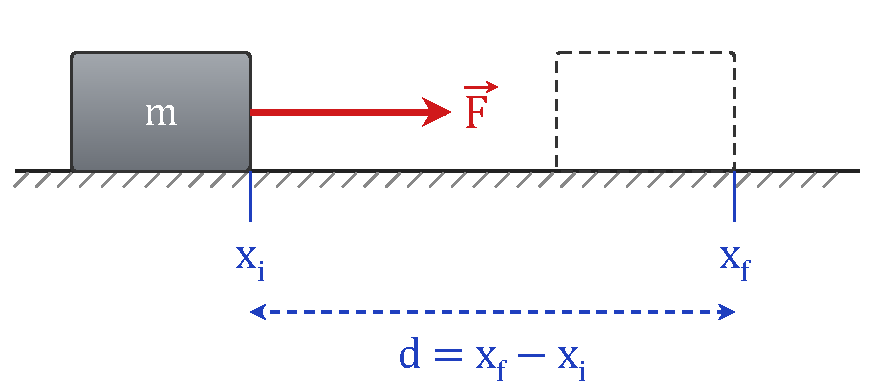
\includegraphics[width=0.7\textwidth]{Figuras_SVG_ES/pdf/U4_trabajo_desplazamiento.pdf}
    \caption{Representación del trabajo}
    \label{fig:trabajo}
\end{figure}
Cuando varias fuerzas actúan sobre el mismo cuerpo, el trabajo realizado por esas fuerzas es el mismo que el trabajo realizado por su resultante (la suma de todas ellas), es decir:
\begin{centeredequation}
    \Sigma F = F_1 + F_2 + \dots
\end{centeredequation}
Por lo tanto, la expresión anterior se convierte en:
\begin{centeredequation}
    W = \Sigma F \cdot d
    \label{eq:trabajo_2}
\end{centeredequation}
\begin{remark}
    El trabajo es una forma de energía y, por tanto, su unidad en el SI es el julio.
\end{remark}

\begin{exercise}
    Calcula el trabajo realizado por un burro cuando ejerce una fuerza de 2000 N sobre un carro y lo arrastra durante 400 metros.
    \begin{solu}
        El trabajo se calcula mediante la fórmula:
        \[
            W = F \cdot d
        \]
        Donde:
        \begin{itemize}
            \item $F = \qty{2000}{\newton}$ (fuerza aplicada)
            \item $d = \qty{400}{\metre}$ (desplazamiento)
        \end{itemize}
        Sustituyendo los valores:
        \[
            W = 2000 \times 400 = \qty{800000}{\joule} = \qty{800}{\kilo\joule}
        \]
        \textbf{Respuesta:} El burro realiza \qty{800}{\kilo\joule} de trabajo.
    \end{solu}
\end{exercise}

\begin{exercise}
    Un estudiante empuja una caja con una fuerza de 80 N y la mueve \qty{5}{\metre} en la misma dirección que la fuerza. Calcula el trabajo realizado.
    \begin{solu}
        Usando la fórmula del trabajo:
        \[
            W = F \cdot d = 80 \times 5 = \qty{400}{\joule}
        \]
        \textbf{Respuesta:} El trabajo realizado es \qty{400}{\joule}.
    \end{solu}
\end{exercise}

\begin{exercise}
    Un coche es empujado por cuatro personas que ejercen una fuerza total de \qty{600}{\newton}. Si el coche se mueve 8 metros, ¿qué trabajo han realizado?
    \begin{solu}

        \[
            W = F \cdot d = 600 \times 8 = \qty{4800}{\joule} = \qty{4.8}{\kilo\joule}
        \]
        \textbf{Respuesta:} Han realizado \qty{4.8}{\kilo\joule} de trabajo.
    \end{solu}
\end{exercise}

\begin{exercise}
    Una persona arrastra una maleta por el suelo aplicando una fuerza de \qty{45}{\newton} en un desplazamiento de \qty{25}{\metre}. Calcula el trabajo realizado.
    \begin{solu}
        \[
            W = F \cdot d = 45 \times 25 = \qty{1125}{\joule} = \qty{1.125}{\kilo\joule}
        \]
        \textbf{Respuesta:} El trabajo realizado es \qty{1.125}{\kilo\joule}.
    \end{solu}
\end{exercise}

\begin{exercise}
    Encuentra el trabajo neto necesario para mover un bloque de \qty{10}{\kilo\gram} cuando el cuerpo se desplaza 3 metros, con fuerzas $F_1 = \qty{80}{\newton}$ y $F_2 = \qty{15}{\newton}$ actuando en la misma dirección.
    \begin{solu}
        Primero, calculamos la fuerza neta:
        \[
            F_{net} = F_1 + F_2 = 80 + 15 = \qty{95}{\newton}
        \]
        Después, calculamos el trabajo:
        \[
            W = F_{net} \cdot d = 95 \times 3 = \qty{285}{\joule}
        \]
        \textbf{Respuesta:} El trabajo neto es \qty{285}{\joule}.
    \end{solu}
\end{exercise}

\begin{exercise}
    Un albañil utiliza una polea para levantar una masa de 50 kg hasta una altura de 10 m. ¿Qué trabajo se ha realizado? (Datos: $g = \qty{9.8}{\mpss}$)
    \begin{solu}
        Primero, calculamos el peso (fuerza):
        \[
            F = m \cdot g = 50 \times 9.8 = \qty{490}{\newton}
        \]
        Después, calculamos el trabajo:
        \[
            W = F \cdot h = 490 \times 10 = \qty{4900}{\joule} = \qty{4.9}{\kilo\joule}
        \]
        \textbf{Respuesta:} El trabajo realizado es \qty{4.9}{\kilo\joule}.
    \end{solu}
\end{exercise}


\section{Energía cinética}

La energía cinética es la energía que posee un cuerpo cuando está en movimiento.
La expresión matemática de la energía cinética es:

\vspace{12pt}
\begin{centeredequation}
    \eqnmarkbox[red]{energiacinetica}{E_k}
    =
    \dfrac{1}{2}
    \eqnmarkbox[blue]{masa}{m}
    \cdot
    \eqnmarkbox[mygreen]{velocidad}{v^2}
    \label{eq:energia_cinetica}
\end{centeredequation}
\annotate[yshift=1em]{left}{energiacinetica}{Energía cinética}
\annotate[yshift=1em]{}{masa}{masa}
\annotate[yshift=-1em]{below,left}{velocidad}{velocidad}
\vspace{12pt}


\begin{exercise}
    Un coche de 1000 kg viaja a una velocidad de 20 m/s. Calcula su energía cinética.
    \begin{solu}
        La fórmula de la energía cinética es:
        \[
            E_k = \frac{1}{2}mv^2
        \]
        Donde $m = \qty{1000}{\kilo\gram}$ y $v = \qty{20}{\mps}$:
        \[
            E_k = \frac{1}{2} \times 1000 \times 20^2 = \frac{1}{2} \times 1000 \times 400 = \qty{200000}{\joule} = \qty{200}{\kilo\joule}
        \]
        \textbf{Respuesta:} La energía cinética es \qty{200}{\kilo\joule}.
    \end{solu}
\end{exercise}

\begin{exercise}
    Una pelota de 0,5 kg se mueve con una velocidad de 10 m/s. ¿Cuál es su energía cinética?
    \begin{solu}
        \[
            E_k = \frac{1}{2}mv^2 = \frac{1}{2} \times 0.5 \times 10^2 = 0.25 \times 100 = \qty{25}{\joule}
        \]
        \textbf{Respuesta:} La energía cinética es \qty{25}{\joule}.
    \end{solu}
\end{exercise}

\begin{exercise}
    Si un objeto de 4 kg tiene una energía cinética de 200 J, ¿a qué velocidad se mueve?
    \begin{solu}
        A partir de $E_k = \frac{1}{2}mv^2$, despejamos $v$:
        \[
            v = \sqrt{\frac{2E_k}{m}} = \sqrt{\frac{2 \times 200}{4}} = \sqrt{\frac{400}{4}} = \sqrt{100} = \qty{10}{\mps}
        \]
        \textbf{Respuesta:} El objeto se mueve a \qty{10}{\mps}.
    \end{solu}
\end{exercise}

\begin{exercise}
    ¿Cuál es la velocidad de un atleta de 80 kg que tiene una energía cinética de 8000 J?
    \begin{solu}
        \[
            v = \sqrt{\frac{2E_k}{m}} = \sqrt{\frac{2 \times 8000}{80}} = \sqrt{\frac{16000}{80}} = \sqrt{200} \approx \qty{14.14}{\mps}
        \]
        \textbf{Respuesta:} El atleta se mueve a aproximadamente \qty{14.14}{\mps}.
    \end{solu}
\end{exercise}


\section{Energía potencial}

Tenemos dos tipos de energía potencial: la energía potencial gravitatoria y la energía potencial elástica.

\subsection{Energía potencial gravitatoria}

Esta energía es consecuencia de la posición de un cuerpo (altura).
La expresión matemática de la energía potencial es:

\vspace{6pt}
\begin{centeredequation}
    \eqnmarkbox[red]{energiapotencial}{E_p}
    =
    \eqnmarkbox[blue]{masa}{m}
    \cdot
    \eqnmarkbox[mygreen]{gravedad}{g}
    \cdot
    \eqnmarkbox[myOrange]{altura}{h}
    \label{eq:energia_potencial}
\end{centeredequation}
\annotate[yshift=1em]{left}{energiapotencial}{Energía potencial}
\annotate[yshift=1em]{}{masa}{masa}
\annotate[yshift=-1em]{below,left}{gravedad}{gravedad}
\annotate[yshift=-1em]{below,right}{altura}{altura}
\vspace{12pt}


\begin{remark}
    A la energía potencial gravitatoria se la conoce habitualmente simplemente como energía potencial.
\end{remark}



\begin{exercise}
    Un libro de 2 kg está en una estantería a 1,5 m de altura. Calcula su energía potencial gravitatoria. (Datos: $g = 9.8$ m/s$^2$)
    \begin{solu}
        La fórmula de la energía potencial gravitatoria es:
        \[
            E_p = mgh
        \]
        Donde $m = \qty{2}{\kilo\gram}$, $g = \qty{9.8}{\mpss}$, y $h = \qty{1.5}{\metre}$:
        \[
            E_p = 2 \times 9.8 \times 1.5 = \qty{29.4}{\joule}
        \]
        \textbf{Respuesta:} La energía potencial es \qty{29.4}{\joule}.
    \end{solu}
\end{exercise}

\begin{exercise}
    Una maceta de 5 kg está situada en un balcón a 12 m del suelo. ¿Cuál es su energía potencial gravitatoria?
    \begin{solu}
        \[
            E_p = mgh = 5 \times 9.8 \times 12 = \qty{588}{\joule}
        \]
        \textbf{Respuesta:} La energía potencial es \qty{588}{\joule}.
    \end{solu}
\end{exercise}

\begin{exercise}
    Si un objeto tiene una energía potencial de 600 J y está situado a 3 m de altura, ¿cuál es su masa?
    \begin{solu}
        A partir de $E_p = mgh$, despejamos $m$:
        \[
            m = \frac{E_p}{gh} = \frac{600}{9.8 \times 3} = \frac{600}{29.4} \approx \qty{20.41}{\kilo\gram}
        \]
        \textbf{Respuesta:} La masa es aproximadamente \qty{20.41}{\kilo\gram}.
    \end{solu}
\end{exercise}

\begin{exercise}
    ¿A qué altura debe elevarse un objeto de 2 kilogramos para que su energía potencial sea de 125 J?
    \begin{solu}
        A partir de $E_p = mgh$, despejamos $h$:
        \[
            h = \frac{E_p}{mg} = \frac{125}{2 \times 9.8} = \frac{125}{19.6} \approx \qty{6.38}{\metre}
        \]
        \textbf{Respuesta:} El objeto debe elevarse a aproximadamente \qty{6.38}{\metre}.
    \end{solu}
\end{exercise}


\section{Energía mecánica}

La energía mecánica es la suma de la energía cinética y la energía potencial.

\begin{centeredequation}
    E_m = E_k + E_p
    \label{eq:energia_mecanica}
\end{centeredequation}

\begin{exercise}
    Calcula la energía de los siguientes objetos:
    \begin{enumerate}[label=\alph*)]
\item Un coche de 1200 kg que viaja a una velocidad de \qty{6}{\mps}
\item Un marco de fotos de 450 gramos situado a 1,75 metros del suelo.
\item Una pelota de tenis de 60 gramos con una velocidad de \qty{65}{\mps} y una altura de 1,25 metros.
    \end{enumerate}
    \begin{solu}
        a) Solo energía cinética:
        \[
            E_k = \frac{1}{2} \times 1200 \times 6^2 = \frac{1}{2} \times 1200 \times 36 = \qty{21600}{\joule} = \qty{21.6}{\kilo\joule}
        \]
        b) Solo energía potencial (convertimos a kg: 450 g = 0,45 kg):
        \[
            E_p = 0.45 \times 9.8 \times 1.75 = \qty{7.72}{\joule}
        \]
        c) Energía cinética y potencial (convertimos a kg: 60 g = 0,06 kg):
        \[
            E_k = \frac{1}{2} \times 0.06 \times 65^2 = \frac{1}{2} \times 0.06 \times 4225 = \qty{126.75}{\joule}
        \]
        \[
            E_p = 0.06 \times 9.8 \times 1.25 = \qty{0.735}{\joule}
        \]
        \[
            E_M = E_k + E_p = 126.75 + 0.735 = \qty{127.49}{\joule}
        \]
        \textbf{Respuestas:} a) \qty{21.6}{\kilo\joule}, b) \qty{7.72}{\joule}, c) \qty{127.49}{\joule}
    \end{solu}
\end{exercise}

\begin{exercise}
    Encuentra la energía mecánica de un águila de 2500 gramos que vuela a una velocidad de \qty{100}{\kmph} y a una altura de 250 m.
    \begin{solu}
        Primero, convertimos las unidades:
        \begin{itemize}
            \item Masa: 2500 g = 2,5 kg
            \item Velocidad: 100 km/h = $\frac{100 \times 1000}{3600} = \qty{27.78}{\mps}$
        \end{itemize}
        Calculamos la energía cinética:
        \[
            E_k = \frac{1}{2} \times 2.5 \times 27.78^2 = \frac{1}{2} \times 2.5 \times 771.73 = \qty{964.66}{\joule}
        \]

        Calculamos la energía potencial:
        \[
            E_p = 2.5 \times 9.8 \times 250 = \qty{6125}{\joule}
        \]

        Energía mecánica total:
        \[
            E_M = E_k + E_p = 964.66 + 6125 = \qty{7089.66}{\joule} \approx \qty{7.09}{\kilo\joule}
        \]
        \textbf{Respuesta:} La energía mecánica es aproximadamente \qty{7.09}{\kilo\joule}.
    \end{solu}
\end{exercise}

\begin{exercise}
    De las siguientes situaciones, ¿cuál tendrá la mayor energía mecánica?:
    \begin{enumerate}[label=\alph*)]
\item Una roca de 10 kg a una altura de 5 metros.
\item Una roca de 5 kg a una altura de 10 metros.
\item Un dron de 250 gramos que vuela cerca del suelo a una velocidad de \qty{25}{\mps}
\item Una piedra de 500 gramos a una altura de 250 metros y una velocidad de \qty{10}{\mps}
    \end{enumerate}
    \begin{solu}
        a) $E_p = 10 \times 9.8 \times 5 = \qty{490}{\joule}$

        b) $E_p = 5 \times 9.8 \times 10 = \qty{490}{\joule}$

        c) $E_k = \frac{1}{2} \times 0.25 \times 25^2 = \frac{1}{2} \times 0.25 \times 625 = \qty{78.13}{\joule}$

        d) $E_k = \frac{1}{2} \times 0.5 \times 10^2 = 25$ J; $E_p = 0.5 \times 9.8 \times 250 = 1225$ J; $E_M = \qty{1250}{\joule}$

        \textbf{Respuesta:} La opción d) tiene la mayor energía mecánica con \qty{1250}{\joule}.
    \end{solu}
\end{exercise}

\begin{exercise}
    Una pelota de 0,4 kg está a una altura de 5 m y se mueve con una velocidad de 8 m/s. Calcula:
    \begin{enumerate}
        \item Su energía potencial
        \item Su energía cinética
        \item Su energía mecánica total
    \end{enumerate}
    \begin{solu}
        1. Energía potencial:
        \[
            E_p = 0.4 \times 9.8 \times 5 = \qty{19.6}{\joule}
        \]
        2. Energía cinética:
        \[
            E_k = \frac{1}{2} \times 0.4 \times 8^2 = 0.2 \times 64 = \qty{12.8}{\joule}
        \]
        3. Energía mecánica total:
        \[
            E_M = E_p + E_k = 19.6 + 12.8 = \qty{32.4}{\joule}
        \]
        \textbf{Respuestas:} 1) \qty{19.6}{\joule}, 2) \qty{12.8}{\joule}, 3) \qty{32.4}{\joule}
    \end{solu}
\end{exercise}

\begin{exercise}
    Un pájaro de 0,2 kg vuela a una altura de 15 m con una velocidad de 12 m/s. Determina su energía mecánica total.
    \begin{solu}
        Energía cinética:
        \[
            E_k = \frac{1}{2} \times 0.2 \times 12^2 = 0.1 \times 144 = \qty{14.4}{\joule}
        \]
        Energía potencial:
        \[
            E_p = 0.2 \times 9.8 \times 15 = \qty{29.4}{\joule}
        \]
        Energía mecánica total:
        \[
            E_M = 14.4 + 29.4 = \qty{43.8}{\joule}
        \]
        \textbf{Respuesta:} La energía mecánica total es \qty{43.8}{\joule}.
    \end{solu}
\end{exercise}


\section{Principio de conservación de la energía mecánica}


\begin{dBox}
    \textbf{El principio de conservación de la energía mecánica dice}: la energía mecánica al principio (fijamos un punto inicial, representado en la fórmula con \( i \)) será igual a la energía mecánica al final (fijamos el punto final, representado en la fórmula con \( f \))
\end{dBox}

Matemáticamente, este principio se puede expresar como:
\begin{centeredequation}
    E_{m,i} = E_{m,f}
    \label{eq:conservacion_energia}
\end{centeredequation}
Esta expresión también se puede escribir como:
\begin{centeredequation}
    E_{p,i} + E_{c,i}  = E_{p,f} + E_{c,f}
    \label{eq:conservacion_energia_semidesarrollada}
\end{centeredequation}
Si desarrollamos aún más esta expresión, obtenemos:
\begin{centeredequation}
    m\cdot g \cdot h_i + \dfrac{1}{2} \cdot m\ v_i^2 = m\cdot g \cdot h_f + \dfrac{1}{2} \cdot m\ v_f^2
    \label{eq:conservacion_energia_desarrollada}
\end{centeredequation}

\begin{exercise}
    Una esfera metálica de 50 kg se deja caer desde una altura de 8 metros hasta el suelo.
    \begin{enumerate}[label=\alph*)]
\item Calcula la energía mecánica que tiene en el momento en que se deja caer.
\item ¿Con qué velocidad llega al suelo?
    \end{enumerate}
    \begin{solu}
        a) En el momento de la suelta, toda la energía es potencial:
        \[
            E_M = E_p = mgh = 50 \times 9.8 \times 8 = \qty{3920}{\joule}
        \]
        b) Por conservación de la energía, a nivel del suelo toda la energía es cinética:
        \[
            E_k = E_M \Rightarrow \frac{1}{2}mv^2 = 3920
        \]
        \[
            v = \sqrt{\frac{2 \times 3920}{50}} = \sqrt{\frac{7840}{50}} = \sqrt{156.8} \approx \qty{12.52}{\mps}
        \]
        Alternativamente: $v = \sqrt{2gh} = \sqrt{2 \times 9.8 \times 8} = \sqrt{156.8} \approx \qty{12.52}{\mps}$
        \textbf{Respuestas:} a) \qty{3920}{\joule}, b) \qty{12.52}{\mps}
    \end{solu}
\end{exercise}

\begin{exercise}
    Desde una altura de \qty{15}{\metre}, un objeto de masa \qty{3}{\kilo\gram} se lanza verticalmente hacia abajo con una velocidad inicial de \qty{2}{\mps}. Si no hay resistencia del aire, encuentra:
    \begin{enumerate}[label=\alph*)]
\item La energía cinética a 5 metros sobre el suelo.
\item La velocidad en ese momento y la velocidad con la que llega al suelo.
    \end{enumerate}
    \begin{solu}
        Energía inicial (a h = 15 m):
        \[
            E_k = \frac{1}{2} \times 3 \times 2^2 = \qty{6}{\joule}
        \]
        \[
            E_p = 3 \times 9.8 \times 15 = \qty{441}{\joule}
        \]
        \[
            E_{M,initial} = 6 + 441 = \qty{447}{\joule}
        \]
        a) A h = 5 m:
        \[
            E_p = 3 \times 9.8 \times 5 = \qty{147}{\joule}
        \]
        \[
            E_k = E_M - E_p = 447 - 147 = \qty{300}{\joule}
        \]
        b) Velocidad a h = 5 m:
        \[
            v = \sqrt{\frac{2E_k}{m}} = \sqrt{\frac{2 \times 300}{3}} = \sqrt{200} \approx \qty{14.14}{\mps}
        \]
        Velocidad en el suelo (h = 0):
        \[
            E_k = E_M = 447 \text{ J}
        \]
        \[
            v = \sqrt{\frac{2 \times 447}{3}} = \sqrt{298} \approx \qty{17.26}{\mps}
        \]
        \textbf{Respuestas:} a) \qty{300}{\joule}, b) \qty{14.14}{\mps} a 5 m de altura, \qty{17.26}{\mps} en el suelo
    \end{solu}
\end{exercise}

\begin{exercise}
    En un tobogán de 2 metros de altura hay un niño de 25 kg. ¿Con qué velocidad llegaría al suelo al deslizarse?
    \begin{solu}
        Por conservación de la energía:
        \[
            E_{p,initial} = E_{k,final}
        \]
        \[
            mgh = \frac{1}{2}mv^2
        \]
        \[
            v = \sqrt{2gh} = \sqrt{2 \times 9.8 \times 2} = \sqrt{39.2} \approx \qty{6.26}{\mps}
        \]
        \textbf{Respuesta:} El niño llega al suelo a aproximadamente \qty{6.26}{\mps}.
    \end{solu}
\end{exercise}

\begin{exercise}
    Una pelota de 0,5 kg se deja caer desde una ventana a 30 m sobre la calle. Calcula:
    \begin{enumerate}[label=\alph*)]
\item La energía potencial respecto al suelo en el momento de la suelta.
\item La energía cinética en el momento en que llega al suelo.
\item La velocidad con la que golpea el suelo.
    \end{enumerate}
    \begin{solu}
        a) Energía potencial en el momento de la suelta:
        \[
            E_p = 0.5 \times 9.8 \times 30 = \qty{147}{\joule}
        \]
        b) Por conservación de la energía, toda la energía potencial se convierte en cinética:
        \[
            E_k = \qty{147}{\joule}
        \]
        c) Velocidad en el suelo:
        \[
            v = \sqrt{2gh} = \sqrt{2 \times 9.8 \times 30} = \sqrt{588} \approx \qty{24.25}{\mps}
        \]
        \textbf{Respuestas:} a) \qty{147}{\joule}, b) \qty{147}{\joule}, c) \qty{24.25}{\mps}
    \end{solu}
\end{exercise}

\begin{exercise}
    En lo alto de una montaña rusa, un vagón y sus ocupantes con una masa total de 1000 kg están a una altura de 50 metros sobre el suelo y tienen una velocidad de \qty{5}{\mps}.
    \begin{enumerate}[label=\alph*)]
\item ¿Qué velocidad tendrá el vagón cuando llegue a la siguiente cima, que está a una altura de 25 metros sobre el suelo?
\item Si la velocidad que tiene en la siguiente cima es de \qty{20}{\mps}, ¿cuál es el trabajo realizado por el rozamiento entre las ruedas y los raíles?
    \end{enumerate}
    \begin{solu}
        Energía inicial (\( h_1 = \qty{50}{\metre} \), \( v_1 = \qty{5}{\metre\per\second} \)):
        \[
            E_{M1} = \frac{1}{2} \times 1000 \times 5^2 + 1000 \times 9.8 \times 50 = 12500 + 490000 = \qty{502500}{\joule}
        \]
        a) Sin rozamiento, a \( h_2 = \qty{25}{\metre} \):
        \[
            E_p = 1000 \times 9.8 \times 25 = \qty{245000}{\joule}
        \]
        \[
            E_k = E_{M1} - E_p = 502500 - 245000 = \qty{257500}{\joule}
        \]
        \[
            v = \sqrt{\frac{2 \times 257500}{1000}} = \sqrt{515} \approx \qty{22.69}{\mps}
        \]
        b) Energía real en \( h_2 \) con \( v_2 \) = \qty{20}{\metre\per\second}:
        \[
            E_{M2} = \frac{1}{2} \times 1000 \times 20^2 + 245000 = 200000 + 245000 = \qty{445000}{\joule}
        \]
        Trabajo realizado por el rozamiento (negativo porque se opone al movimiento):
        \[
            W_{friction} = E_{M2} - E_{M1} = 445000 - 502500 = \qty{-57500}{\joule}
        \]
        \textbf{Respuestas:} a) \qty{22.69}{\mps}, b) \qty{-57500}{\joule} (o \qty{57500}{\joule} de energía perdida)
    \end{solu}
\end{exercise}

\begin{exercise}
    Una pelota de 0,3 kg se deja caer desde una altura de 10 m. Calcula:
    \begin{enumerate}
        \item La energía mecánica inicial
        \item La velocidad con la que llega al suelo
        \item La energía cinética justo antes de tocar el suelo
    \end{enumerate}
    \begin{solu}
        1. Energía mecánica inicial (toda potencial):
        \[
            E_M = mgh = 0.3 \times 9.8 \times 10 = \qty{29.4}{\joule}
        \]
        2. Velocidad en el suelo:
        \[
            v = \sqrt{2gh} = \sqrt{2 \times 9.8 \times 10} = \sqrt{196} = \qty{14}{\mps}
        \]
        3. Energía cinética en el suelo (igual a la energía mecánica inicial):
        \[
            E_k = \qty{29.4}{\joule}
        \]
        \textbf{Respuestas:} 1) \qty{29.4}{\joule}, 2) \qty{14}{\mps}, 3) \qty{29.4}{\joule}
    \end{solu}
\end{exercise}

\begin{exercise}
    Un péndulo tiene una masa de 0,5 kg y se suelta desde una altura de 2 m. Si no hay rozamiento:
    \begin{enumerate}
        \item ¿Cuál es su energía potencial inicial?
        \item ¿Cuál será su velocidad máxima en el punto más bajo?
        \item ¿Qué energía cinética tendrá cuando esté a una altura de 1 m?
    \end{enumerate}
    \begin{solu}
        1. Energía potencial inicial:
        \[
            E_p = 0.5 \times 9.8 \times 2 = \qty{9.8}{\joule}
        \]
        2. Velocidad máxima en el punto más bajo (h = 0):
        \[
            v = \sqrt{2gh} = \sqrt{2 \times 9.8 \times 2} = \sqrt{39.2} \approx \qty{6.26}{\mps}
        \]
        3. A h = 1 m:
        \[
            E_p = 0.5 \times 9.8 \times 1 = \qty{4.9}{\joule}
        \]
        \[
            E_k = E_M - E_p = 9.8 - 4.9 = \qty{4.9}{\joule}
        \]
        \textbf{Respuestas:} 1) \qty{9.8}{\joule}, 2) \qty{6.26}{\mps}, 3) \qty{4.9}{\joule}
    \end{solu}
\end{exercise}

\begin{exercise}
    Un esquiador de 70 kg parte del reposo desde la cima de una pendiente situada a 20 m de altura. Si despreciamos el rozamiento, ¿con qué velocidad llegará a la base de la pendiente?
    \begin{solu}
        Usando la conservación de la energía:
        \[
            v = \sqrt{2gh} = \sqrt{2 \times 9.8 \times 20} = \sqrt{392} \approx \qty{19.80}{\mps}
        \]
        \textbf{Respuesta:} El esquiador llegará a la base a aproximadamente \qty{19.80}{\mps}.
    \end{solu}
\end{exercise}


\section{Potencia}

Otra magnitud importante es la potencia (\( P \)). La potencia se puede definir como la energía (\( E \)) o el trabajo (\( W \)) realizado por unidad de tiempo (\( t \)), y su expresión matemática es:
\begin{centeredequation}
    P = \dfrac{E}{t}
    \label{eq:potencia_energia}
\end{centeredequation}
o de forma equivalente:
\begin{centeredequation}
    P = \dfrac{W}{t}
    \label{eq:potencia_trabajo}
\end{centeredequation}

La unidad de potencia en el Sistema Internacional es el Vatio (\unit{\watt}). Otra unidad de potencia muy utilizada es el caballo de vapor (CV), donde
\( 1\ HP = \qty{735}{\watt} \)

\begin{exercise}
    Una grúa levanta una carga de $500\,\text{kg}$ hasta una altura de $20\,\text{metros}$ en $10\,\text{segundos}$. Calcula la potencia desarrollada por la grúa. (Usa $g = 9.8\,\text{m/s}^2$).
    \begin{solu}
        Primero, calculamos el trabajo realizado (energía potencial): $W = m \cdot g \cdot h$ \\
        $W = 500\,\text{kg} \cdot 9.8\,\text{m/s}^2 \cdot 20\,\text{m} = 98,000\,\text{J}$ \\
        Ahora, hallamos la potencia: $P = \frac{W}{t} = \frac{98,000\,\text{J}}{10\,\text{s}} = \mathbf{9800\,\text{W}}$
    \end{solu}
\end{exercise}

\begin{exercise}
    Un motor eléctrico tiene una potencia de $1200\,\text{W}$. ¿Cuánto tiempo tardará en realizar $18,000\,\text{J}$ de trabajo?
    \begin{solu}
        Usando la fórmula $P = \frac{W}{t}$, despejamos $t$: \\
        $t = \frac{W}{P} = \frac{18,000\,\text{J}}{1200\,\text{W}} = \mathbf{15\,\text{segundos}}$
    \end{solu}
\end{exercise}

\begin{exercise}
    Un estudiante con una masa de $60\,\text{kg}$ sube una escalera de $5\,\text{metros}$ de altura en $12\,\text{segundos}$.
    Calcula la potencia generada.
    \begin{solu}
        $W = m \cdot g \cdot h = 60\,\text{kg} \cdot 9.8\,\text{m/s}^2 \cdot 5\,\text{m} = 2940\,\text{J}$ \\
        $P = \frac{2940\,\text{J}}{12\,\text{s}} = \mathbf{245\,\text{W}}$
    \end{solu}
\end{exercise}

\begin{exercise}
    Una bombilla tiene una potencia de $60\,\text{W}$.
    Si permanece encendida durante $2\,\text{horas}$, ¿cuánta energía total (en julios) consume?
    \begin{solu}
        Primero, convertimos el tiempo a segundos: $2\,\text{h} \cdot 3600\,\text{s/h} = 7200\,\text{s}$ \\
        $E = P \cdot t = 60\,\text{W} \cdot 7200\,\text{s} = \mathbf{432,000\,\text{J}}$ (o $4.32 \cdot 10^5\,\text{J}$)
    \end{solu}
\end{exercise}


\section{Consumo energético doméstico}

La Figura \ref{fig:factura_luz} muestra la información que se suele encontrar en una factura de la luz.

\begin{figure}[H]
    \centering
%    \includegraphics[scale=0.9]{images/energia/factura_luz}
    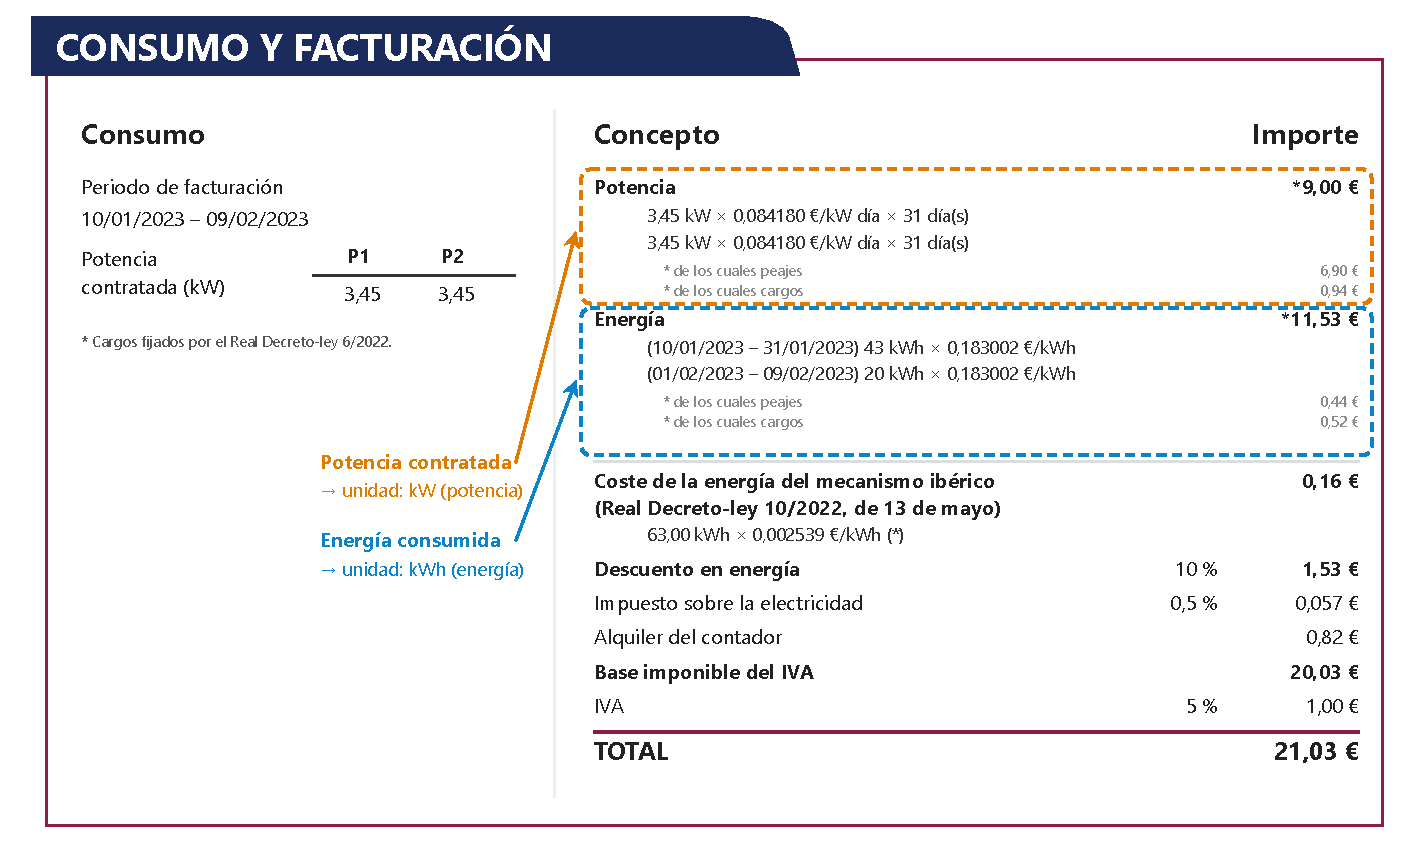
\includegraphics[width=\textwidth]{Figuras_SVG_ES/pdf/U4_factura_luz.pdf}
    \caption{Información que aparece en una factura de la luz}
    \label{fig:factura_luz}
\end{figure}

Primero, vemos que debemos pagar por la potencia contratada.
Como hemos visto, la potencia es la energía suministrada por unidad de tiempo, y su unidad en el SI es el vatio (\unit{\watt}).

En este caso, la potencia contratada es de \qty{3.45}{\kilo\watt}.
F
\begin{remark}
    Aquí vemos una conversión de unidades usando factores de conversión para calcular el precio que debemos pagar tras 31 días por la potencia contratada.
\end{remark}
\begin{example}
    Calcula el precio que tenemos que pagar por 31 días usando factores de conversión. A continuación, se muestra la energía consumida así como el precio a pagar.
    En este caso, es \( 0.084180 \dfrac{\text{€}}{\unit{\kwh}} \) y vemos que primero se consumieron \qty{43}{\kwh}, seguidos de \qty{20}{\kwh}.
\end{example}


\begin{remark}
    Es importante no confundir \unit{\kwh}, que es una unidad de energía, con \unit{\watt}, que es una unidad de potencia.\\
    Calcula la equivalencia entre \unit{\kwh} y julios.
\end{remark}

\begin{exercise}
    Debes revisar una factura de electricidad doméstica y calcular el coste de tener tres electrodomésticos encendidos durante un cierto periodo de tiempo.
\end{exercise}


\section{Fuentes de energía}

Una \textbf{fuente de energía} es un recurso natural del cual se puede obtener energía y transformarla en otras formas.
Según su capacidad de regeneración, tenemos:

\begin{enumerate}[label=\numberballmDarkTeal]
\item \negsubro{Renovables}.
La tasa de regeneración iguala a la tasa de consumo, y pueden considerarse inagotables.
\begin{itemize}
    \item Energía hidroeléctrica.
    \item Energía solar.
    \item Energía geotérmica.
    \item Biomasa.
    \item Energía marina.
    \item Energía eólica.
\end{itemize}
\item \negsubro{No renovables}
\end{enumerate}


\section{Calor y temperatura}

A menudo se confunden los términos calor y temperatura.

\textbf{Calor} es la cantidad de energía transferida de un cuerpo a otro debido a una diferencia de temperatura.
Para que exista calor, dos cuerpos deben estar en contacto.
Dado que el calor es una forma de energía, su unidad en el SI es el julio.

\textbf{Temperatura} es la medida de la energía cinética de las moléculas de una sustancia.
La unidad del SI es el Kelvin, aunque los grados Celsius se usan ampliamente.

\begin{centeredequation}
    \unit{\kelvin} = \unit{\degreeCelsius} + 273
\end{centeredequation}
\begin{centeredequation}
    \unit{\degreeCelsius} = \unit{\kelvin} - 273
\end{centeredequation}

\begin{remark}
    Podemos decir que la temperatura es muy alta pero el calor es bajo.\\
    ¿Podrías explicar por qué?
\end{remark}

\begin{exercise}
    Explica por qué la temperatura en la superficie del sol es muy alta, mientras que su calor no es tan alto en comparación.
    Busca la respuesta en internet, incluyendo fuentes relevantes.
\end{exercise}

%\section{Vocabulario}
%
%
%\begin{vocabulary}[Energy]
%The capacity to do work or produce change in a physical system. \newline
%\textbf{Translation to Spanish}: Energía \newline
%% Line 10
%\end{vocabulary}
%
%
%\begin{vocabulary}[Kinetic Energy]
%The energy possessed by an object due to its motion. \newline
%\textbf{Translation to Spanish}: Energía cinética \newline
%% Line 52
%\end{vocabulary}
%
%
%\begin{vocabulary}[Potential Energy]
%Stored energy associated with the position or configuration of an object. \newline
%\textbf{Translation to Spanish}: Energía potencial \newline
%% Line 73
%\end{vocabulary}
%
%
%\begin{vocabulary}[Mechanical Energy]
%The sum of kinetic and potential energy in a system. \newline
%\textbf{Translation to Spanish}: Energía mecánica \newline
%% Line 89
%\end{vocabulary}
%
%
%\begin{vocabulary}[Work]
%The transfer of energy that occurs when a force moves an object through a distance. \newline
%\textbf{Translation to Spanish}: Trabajo \newline
%% Line 132
%\end{vocabulary}
%
%
%\begin{vocabulary}[Power]
%The rate at which work is done or energy is transferred. \newline
%\textbf{Translation to Spanish}: Potencia \newline
%% Line 174
%\end{vocabulary}
%
%
%\begin{vocabulary}[Conservation of Energy]
%A principle stating that energy cannot be created or destroyed, only transformed from one form to another. \newline
%\textbf{Translation to Spanish}: Conservación de la energía \newline
%% Line 214
%\end{vocabulary}
%
%
%\begin{vocabulary}[Thermal Energy]
%The internal energy of a system associated with the random motion of its particles. \newline
%\textbf{Translation to Spanish}: Energía térmica \newline
%% Line 247
%\end{vocabulary}
%
%
%\begin{vocabulary}[Heat]
%The transfer of thermal energy between systems due to a temperature difference. \newline
%\textbf{Translation to Spanish}: Calor \newline
%% Line 281
%\end{vocabulary}
%
%
%\begin{vocabulary}[Temperature]
%A measure of the average kinetic energy of the particles in a substance. \newline
%\textbf{Translation to Spanish}: Temperatura \newline
%% Line 298
%\end{vocabulary}


%----------------------------------------------------------------------------------------
%	SECTIONING EXAMPLES CHAPTER
%----------------------------------------------------------------------------------------

    %\chapterimage{orange3b} % Chapter heading image % --- imagen antigua ---
    \chapterimage{Images/portada_cabeceras/cabecera_general} % Cabecera nueva (las de cada unidad van antes de cada \chapter)
    \chapterspaceabove{6.75cm} % Whitespace from the top of the page to the chapter title on chapter pages
    \chapterspacebelow{7.25cm} % Amount of vertical whitespace from the top margin to the start of the text on chapter pages

%----------------------------------------------------------------------------------------
%	PART CHEMISTRY
%----------------------------------------------------------------------------------------


    \part{Química: Parte A}

    %------------------------------------------------


    \chapterimage{Images/portada_cabeceras/cabecera_U5_sistemas_materiales}
    \chapter{Sistemas Materiales}

    \spacing{1.3}


\section{Sistemas materiales}
Podemos clasificar los sistemas materiales en (ver esquema):
\vspace{12pt}

\esquema{Sistemas materiales}
{\esquema{Sustancias puras}
{\esquema{Elementos}
{\( \bullet \) Hidrógeno
\vspace{6pt}\\
    \( \bullet \) Litio}
\vspace{20pt}\\
\esquema{Compuestos}
{\( \bullet \)\ch{NaCl}
\vspace{6pt}\\
    \( \bullet \)\ch{H2O}
\vspace{6pt}\\
    \( \bullet \)\ch{H2SO4}}
}
\vspace{20pt} \\
\esquema{Mezclas}
{\( \bullet \) Homogéneas
\vspace{6pt}\\
    \( \bullet \) Heterogéneas
}
}

\begin{enumerate}[label=\numberballmDarkTeal]
\item \negsubro{Sustancias puras}: un tipo de materia que tiene una composición constante y propiedades definidas, y que no puede separarse en otras sustancias mediante métodos físicos.
Las sustancias puras pueden dividirse en:
\begin{itemize}
    \item \textbf{Elementos}: formados por un único tipo de átomo.
    \item \textbf{Compuestos}: formados por la unión de dos o más elementos químicos.
\end{itemize}

\item \negsubro{Mezclas}: la combinación de dos o más sustancias puras que pueden separarse mediante métodos físicos.
Las mezclas pueden dividirse en:
\begin{itemize}
    \item \textbf{Mezcla homogénea}: una mezcla en la que los componentes están distribuidos de manera uniforme y no pueden distinguirse a simple vista.
    \item \textbf{Mezcla heterogénea}: una mezcla en la que los componentes pueden distinguirse.
\end{itemize}

\end{enumerate}


\section{Disoluciones}

\begin{definition}[Disolución]
    Es un sistema homogéneo formado por dos o más sustancias puras en distintas proporciones.
\end{definition}

Los componentes de una disolución son:
\begin{itemize}
    \item \textbf{Disolvente}. La sustancia en mayor cantidad.
    \item \textbf{Soluto}. La sustancia en menor cantidad. Puede haber más de un soluto.
    \item \textbf{Disolución}. La mezcla del soluto(s) y el disolvente.
\end{itemize}

Por ejemplo, en una disolución de agua y azúcar, el disolvente es el agua y el soluto es el azúcar.
En una botella de agua mineral, la etiqueta indica que contiene sodio, calcio, magnesio, etc.
En este caso, el disolvente es el agua, y los solutos son el sodio, el calcio y el magnesio.

\subsection{Concentración de una disolución}

Cuando tenemos una disolución, es fundamental saber cuánto soluto hay en el disolvente.

\begin{definition}[Concentración]
    Es la cantidad de soluto disuelto en una cierta cantidad de disolvente.
\end{definition}

Existen diferentes formas de expresar la concentración. Las principales son:

\begin{enumerate}[label=\numberballmDarkTeal]
\item \negsubro{Porcentaje en masa}.
Nos indica la masa de soluto en cada \qty{100}{\g} de disolución.

\begin{equation}
    \text{\% en masa de soluto} = \dfrac{\text{masa de soluto}}{\text{masa de disolución}}\cdot 100
    \label{eq:porcentaje_masa}
\end{equation}

Importante:
\begin{itemize}
    \item Si hay varios solutos, calculamos el porcentaje de cada uno.
    \item También podemos calcular el porcentaje del disolvente.
    \item Todos los porcentajes juntos deben sumar \num{100}.
\end{itemize}
\end{enumerate}

\begin{example}
    Tenemos una disolución acuosa con sodio y calcio.
    Hay \qty{18}{\g} de sodio, \qty{6}{\g} de calcio, y \qty{100}{\g} de agua.
    Calcula el porcentaje en masa del sodio y del calcio.

    En ambos casos debemos aplicar la ecuación \eqref{eq:porcentaje_masa}.
    En ambos casos tenemos que:

    \begin{equation*}
        \text{\% masa de sodio} = \dfrac{\qty{18}{\g}\text{ de sodio}}{\qty{18}{\g}\text{ de sodio} + \qty{6}{\g}\text{ de calcio} + \qty{100}{\g}\text{ de agua}}\cdot 100 = 14.52 \%
    \end{equation*}

    \begin{equation*}
        \text{\% masa de calcio} = \dfrac{\qty{6}{\g}\text{ de calcio}}{\qty{18}{\g}\text{ de sodio} + \qty{6}{\g}\text{ de calcio} + \qty{100}{\g}\text{ de agua}}\cdot 100 = 4.84 \%
    \end{equation*}

    Si también queremos calcular el porcentaje del disolvente, sería:

    \begin{equation*}
        \text{\% masa de agua} = \dfrac{\qty{100}{\g}\text{ de agua}}{\qty{18}{\g}\text{ de sodio} + \qty{6}{\g}\text{ de calcio} + \qty{100}{\g}\text{ de agua}}\cdot 100 = 80.65 \%
    \end{equation*}
\end{example}

\begin{exercise}
    El acero es una aleación compuesta de hierro, carbono y otros elementos. Una masa de \qty{120}{\g} de acero contiene un 1,8\% de carbono y un 1,2\% de manganeso. Calcula la masa de cada elemento.
    \begin{solu}
        \textbf{Fórmula:} $m_{\text{componente}} = \frac{\% \text{ en masa}}{100} \cdot m_{\text{total}}$ \\
        \textbf{Datos:} $m_{\text{total}} = 120 \text{ g}$; $\%C = 1.8\%$; $\%Mn = 1.2\%$ \\
        \textbf{Solución:}
        \begin{enumerate}
            \item \textbf{Masa de carbono:} $m_{C} = \frac{1.8}{100} \cdot 120 \text{ g} = 2.16 \text{ g}$
            \item \textbf{Masa de manganeso:} $m_{Mn} = \frac{1.2}{100} \cdot 120 \text{ g} = 1.44 \text{ g}$
            \item \textbf{Masa de hierro:} Se calcula restando los demás componentes del total: \\
            $m_{Fe} = 120 \text{ g} - (2.16 \text{ g} + 1.44 \text{ g}) = 116.4 \text{ g}$
        \end{enumerate}
    \end{solu}
\end{exercise}

\begin{exercise}
    Disolvemos 12 g de cloruro de sodio y 13 g de cloruro de potasio en 250 g de agua destilada. Calcula el porcentaje en masa de cada soluto en la disolución final.
    \begin{solu}
        \textbf{Fórmulas:} $m_{\text{total}} = m_{s1} + m_{s2} + m_{\text{disolvente}}$ y $\%m = \frac{m_{\text{soluto}}}{m_{\text{total}}} \cdot 100$ \\
        \textbf{Solución:}
        \begin{enumerate}
            \item \textbf{Masa total:} $12 \text{ g} + 13 \text{ g} + 250 \text{ g} = 275 \text{ g}$.
            \item \textbf{\% NaCl:} $\frac{12 \text{ g}}{275 \text{ g}} \cdot 100 \approx 4.36\%$
            \item \textbf{\% KCl:} $\frac{13 \text{ g}}{275 \text{ g}} \cdot 100 \approx 4.73\%$
        \end{enumerate}
    \end{solu}
\end{exercise}

\begin{exercise}
    Queremos preparar 500 g de una disolución acuosa que contenga un 0,5\% de cloruro de sodio, un 0,3\% de cloruro de potasio y un 0,2\% de nitrato de potasio en masa. ¿Cuánto de cada soluto se necesita? ¿Cuánta agua necesitamos?
    \begin{solu}
        \textbf{Fórmula:} $m_s = \frac{\%m}{100} \cdot m_{\text{total}}$ \\

        \textbf{Datos:} $m_{\text{total}} = 500 \text{ g}$. \\

        \textbf{Solución:}
        \begin{itemize}
            \item $m_{NaCl} = 500 \cdot 0.005 = 2.5 \text{ g}$
            \item $m_{KCl} = 500 \cdot 0.003 = 1.5 \text{ g}$
            \item $m_{KNO_3} = 500 \cdot 0.002 = 1.0 \text{ g}$
            \item \textbf{Masa de agua:} $500 \text{ g} - (2.5 + 1.5 + 1.0) \text{ g} = 495 \text{ g}$
        \end{itemize}
    \end{solu}
\end{exercise}

\begin{exercise}
    ¿Qué significa que una disolución de yodo en alcohol sea del 1\% en masa?
    \begin{solu}
        \textbf{Definición de porcentaje en masa:} Representa las partes de soluto en 100 partes de disolución. \\
        Significa que en cada \textbf{100 g de disolución}, hay exactamente \textbf{1 g de yodo} (soluto) y los \textbf{99 g restantes son alcohol} (disolvente).
    \end{solu}
\end{exercise}

\begin{exercise}
    Utilizamos una mezcla de plomo y estaño en soldadura. Si el porcentaje en masa de plomo es del 66\% y el de estaño del 34\%, ¿qué masas de cada metal fundirías para preparar 250 g de esta aleación?
    \begin{solu}
        \textbf{Fórmula:} $m_{\text{componente}} = \frac{\%m}{100} \cdot m_{\text{total}}$ \\

        \textbf{Datos:} $m_{\text{total}} = 250 \text{ g}$. \\

        \textbf{Solución:}
        \begin{itemize}
            \item Masa de plomo (Pb): $250 \cdot 0.66 = 165 \text{ g}$
            \item Masa de estaño (Sn): $250 \cdot 0.34 = 85 \text{ g}$
        \end{itemize}
        (Comprobación: $165 + 85 = 250 \text{ g}$).
    \end{solu}
\end{exercise}


\begin{exercise}
    El porcentaje en masa de cloruro de potasio en una cierta disolución es del 10\%. ¿Cuánto de este soluto está disuelto en 250 g de disolución?
    \begin{solu}
        \textbf{Fórmula:} $m_s = \frac{\%m}{100} \cdot m_{\text{disolución}}$ \\
        \textbf{Solución:} Aplicamos la definición directamente a la masa total: \\
        $m_{KCl} = 250 \text{ g} \cdot \frac{10}{100} = 25 \text{ g}$ de KCl.
    \end{solu}
\end{exercise}

\begin{exercise}
    Un agua embotellada contiene un 99,8\% en masa de agua y un 0,2\% de dióxido de carbono. Identifica el soluto y el disolvente en esta disolución. ¿Qué masa de dióxido de carbono contendría 1 kg de agua?
    \begin{solu}
        \textbf{Concepto:} Identificar el soluto (menor cantidad) y el disolvente (mayor cantidad). \\
        \textbf{Fórmula de proporción:} $\frac{m_{\text{soluto}}}{m_{\text{disolvente}}} = \frac{\% \text{ soluto}}{\% \text{ disolvente}}$ \\
        \textbf{Solución:}
        \begin{itemize}
            \item \textbf{Identificación:} Soluto = dióxido de carbono ($CO_2$); Disolvente = agua ($H_2O$).
            \item \textbf{Cálculo de la masa:} Tenemos 1 kg (1000 g) de agua. \\
            $m_{CO_2} = \frac{0.2 \text{ g } CO_2}{99.8 \text{ g } H_2O} \cdot 1000 \text{ g } H_2O \approx 2.004 \text{ g}$ de $CO_2$.
        \end{itemize}
    \end{solu}
\end{exercise}

\begin{enumerate}[label=\numberballmDarkTeal,resume]
\item \negsubro{Porcentaje en volumen}.
Nos indica el volumen de soluto en cada \qty{100}{\litre} de disolución.

\begin{equation}
    \text{\% en volumen de soluto} = \dfrac{\text{volumen de soluto}}{\text{volumen de disolución}}\cdot 100
\end{equation}
\end{enumerate}

\begin{example}
    Preparamos una disolución con \qty{100}{\ml} de alcohol, \qty{150}{\ml} de acetona, y \qty{250}{\ml} de agua.
    Calcula el porcentaje en volumen de cada sustancia.

    \begin{equation*}
        \text{\% vol alcohol} = \dfrac{\qty{100}{\ml}\text{ de alcohol}}{\qty{100}{\ml}\text{ de alcohol} + \qty{150}{\ml}\text{ de acetona} + \qty{250}{\ml}\text{ de agua}}\cdot 100 = 20 \%
    \end{equation*}

    \begin{equation*}
        \text{\% vol acetona} = \dfrac{\qty{150}{\ml}\text{ de acetona}}{\qty{100}{\ml}\text{ de alcohol} + \qty{150}{\ml}\text{ de acetona} + \qty{250}{\ml}\text{ de agua}}\cdot 100 = 30 \%
    \end{equation*}

    \begin{equation*}
        \text{\% vol agua} = \dfrac{\qty{250}{\ml}\text{ de agua}}{\qty{100}{\ml}\text{ de alcohol} + \qty{150}{\ml}\text{ de acetona} + \qty{250}{\ml}\text{ de agua}}\cdot 100 = 50 \%
    \end{equation*}
\end{example}

\begin{exercise}
    Se prepara una disolución de éter y cloroformo añadiendo \qty{10}{\mL} de éter a 90 mL de cloroformo. ¿Cuál es el porcentaje en volumen de cada componente?
    \begin{solu}
        \textbf{Fórmulas:} \\
        1. $V_{\text{disolución}} = V_{\text{soluto}} + V_{\text{disolvente}}$ \\
        2. $\%V = \frac{V_{\text{componente}}}{V_{\text{disolución}}} \cdot 100$ \\

        \textbf{Datos:} $V_{\text{éter}} = 10 \text{ mL}$; $V_{\text{cloroformo}} = 90 \text{ mL}$ \\

        \textbf{Solución:}
        \begin{enumerate}
            \item \textbf{Volumen de la disolución:} $V_{\text{total}} = 10 \text{ mL} + 90 \text{ mL} = 100 \text{ mL}$.
            \item \textbf{Porcentaje de éter:} $\%V_{\text{éter}} = \frac{10 \text{ mL}}{100 \text{ mL}} \cdot 100 = 10\%$
            \item \textbf{Porcentaje de cloroformo:} $\%V_{\text{cloro}} = \frac{90 \text{ mL}}{100 \text{ mL}} \cdot 100 = 90\%$
        \end{enumerate}
    \end{solu}
\end{exercise}

\begin{exercise}
    La composición en volumen de los ingredientes activos en un envase de 200 mL de loción corporal es: 2,14\% de aceite de almendras dulces; 2,14\% de aceite de maíz; 4,29\% de aceite de cacahuete y 2,88\% de aceite de copra hidrogenado. Calcula el volumen de cada componente.
    \begin{solu}
        \textbf{Fórmula:} $V_{\text{comp}} = \frac{\%V}{100} \cdot V_{\text{total}}$ \\
        \textbf{Datos:} $V_{\text{total}} = 200 \text{ mL}$. \\
        \textbf{Solución:} Multiplicamos el volumen total por cada porcentaje decimal:
        \begin{itemize}
            \item Aceite de almendras: $200 \cdot 0.0214 = 4.28 \text{ mL}$
            \item Aceite de maíz: $200 \cdot 0.0214 = 4.28 \text{ mL}$
            \item Aceite de cacahuete: $200 \cdot 0.0429 = 8.58 \text{ mL}$
            \item Aceite de copra: $200 \cdot 0.0288 = 5.76 \text{ mL}$
        \end{itemize}
    \end{solu}
\end{exercise}


\begin{exercise}
    Hemos disuelto \qty{25}{\cmcubicos} de alcohol en agua destilada para obtener un volumen total de disolución de \qty{250}{\cmcubicos}.
    \begin{enumerate}[label=\letraminuscula]
        \item ¿Cuál es el volumen del soluto y del disolvente?
        \item Calcula el porcentaje en volumen de cada componente de esta disolución.
    \end{enumerate}
    \begin{solu}
        \textbf{Fórmulas:} $V_{\text{disolvente}} = V_{\text{total}} - V_{\text{soluto}}$ y $\%V = \frac{V_{\text{comp}}}{V_{\text{total}}} \cdot 100$ \\
        \textbf{Solución:}
        \begin{enumerate}[label=\alph*)]
            \item \textbf{Volúmenes:} Soluto = $25 \text{ cm}^3$ (alcohol). \\
            Disolvente = $250 \text{ cm}^3 - 25 \text{ cm}^3 = 225 \text{ cm}^3$ (agua).
            \item \textbf{Porcentajes:} \\
            $\%V_{\text{alcohol}} = \frac{25}{250} \cdot 100 = 10\%$ \\
            $\%V_{\text{agua}} = \frac{225}{250} \cdot 100 = 90\%$
        \end{enumerate}
    \end{solu}
\end{exercise}


\begin{enumerate}[label=\numberballmDarkTeal,resume]
\item \negsubro{Concentración en masa}.
Nos indica la masa de soluto por unidad de volumen de disolución.
Se suele expresar en \unit{\g\per\litre}.

\begin{equation*}
    \text{Concentración en masa} = \dfrac{m_{\text{soluto (g)}}}{V_{\text{disolución (L)}}}
\end{equation*}

No hay que confundirla con la densidad:
\begin{itemize}
    \item La densidad es la masa de una sustancia por unidad de volumen.
    \item La concentración en masa es la masa de soluto por unidad de volumen de la \textbf{disolución}.
\end{itemize}
\end{enumerate}

\begin{example}
    Para preparar una disolución de nitrato de potasio con \qty{20}{\g} de nitrato en agua para obtener un volumen final de disolución de \qty{200}{\ml}. Calcula:
    \begin{enumerate}[label=\letraminuscula]
\item La concentración en masa de la disolución expresada en \unit{\g\per\litre}.

Como el volumen de la disolución se da en \unit{\ml}, lo convertimos a \unit{\litre}. El volumen es entonces \qty{0.2}{\litre}. Si aplicamos:
\begin{equation*}
    \text{Concentración en masa} = \dfrac{m_{\text{soluto (g)}}}{V_{\text{disolución (L)}}} = \dfrac{20}{0.2} = \qty{100}{\g\per\litre}
\end{equation*}

\item Calcula la masa de la disolución si la densidad de esta disolución es \( \rho = \qty{1.09}{\g\per\cubic\centi\metre} \).

Para calcular su masa, despejamos la masa en la ecuación de la densidad:
\begin{equation*}
    \rho = \dfrac{m}{V} \rightarrow m = \rho \cdot V
\end{equation*}
Antes de sustituir en la ecuación, debemos comprobar que tanto la densidad como el volumen están en las mismas unidades, pero sabemos que \( \qty{1}{\ml} = \qty{1}{\cubic\centi\metre} \).
\begin{equation*}
    m = \rho \cdot V = 1.09 \cdot 200 = \qty{218}{\g}
\end{equation*}
    \end{enumerate}
\end{example}

\begin{exercise}
    200 ml de una disolución acuosa contienen 12 g de azúcar. La densidad de esta disolución es \qty{1.022}{\g\per\cmcubicos}.
    \begin{enumerate}[label=\letraminuscula]
        \item Calcula el porcentaje en masa del azúcar.
        \item Calcula la concentración en masa en g/L.
    \end{enumerate}
    \begin{solu}
        \textbf{Fórmulas:} $m_{\text{disolución}} = d \cdot V$; $\%m = \frac{m_s}{m_{\text{disolución}}} \cdot 100$; $C = \frac{m_s}{V(L)}$ \\
        \textbf{Solución:}
        \begin{enumerate}[label=\alph*)]
        \item \textbf{Porcentaje en masa:}
        Primero calculamos la masa total: $m_{\text{total}} = 1.022 \text{ g/cm}^3 \cdot 200 \text{ cm}^3 = 204.4 \text{ g}$. \\
        $\%m = \frac{12 \text{ g}}{204.4 \text{ g}} \cdot 100 \approx 5.87\%$
        \item \textbf{Concentración en g/L:}
        Dividimos la masa del soluto entre el volumen en litros ($200 \text{ mL} = 0.2 \text{ L}$): \\
        $C = \frac{12 \text{ g}}{0.2 \text{ L}} = 60 \text{ g/L}$
        \end{enumerate}
    \end{solu}
\end{exercise}

\begin{exercise}
    Se puede preparar un suero salino isotónico disolviendo 0,9 g de cloruro de sodio en agua hasta obtener 100 mL de disolución.
    Calcula:
    \begin{enumerate}[label=\letraminuscula]
            \item la concentración en masa en g/L de esta disolución.
            \item la masa de cloruro de sodio necesaria para preparar 250 mL de suero salino isotónico.
    \end{enumerate}
    \begin{solu}
        \textbf{Fórmulas:} $C \text{ (g/L)} = \frac{m_{\text{soluto (g)}}}{V_{\text{disolución (L)}}}$ y $m_s = C \cdot V$ \\
        \textbf{Solución:}
        \begin{enumerate}[label=\alph*)]
                \item \textbf{Concentración:} Cambiamos el volumen a litros ($100 \text{ mL} = 0.1 \text{ L}$). \\
                $C = \frac{0.9 \text{ g}}{0.1 \text{ L}} = 9 \text{ g/L}$.
                \item \textbf{Masa para 250 mL:} Cambiamos el volumen ($250 \text{ mL} = 0.25 \text{ L}$). \\
                $m = 9 \text{ g/L} \cdot 0.25 \text{ L} = 2.25 \text{ g}$ de NaCl.
        \end{enumerate}
    \end{solu}
\end{exercise}


\section{Solubilidad}

\begin{definition}[Solubilidad]
        La \textbf{solubilidad} de un soluto a una cierta temperatura y en un cierto disolvente es la cantidad máxima de ese soluto que puede disolverse en \qty{100}{\g} de disolvente.
\end{definition}

A partir de esta definición podemos ver que la solubilidad depende de la temperatura y del disolvente.
Esto significa que la solubilidad cambia cuando cambia la temperatura y cuando cambia el disolvente.

Por ejemplo, si algo no se disuelve a temperatura ambiente, podemos calentarlo.
Esto demuestra que cuando la temperatura aumenta, la solubilidad también aumenta.

Para expresar correctamente la solubilidad, debemos dar el valor de la solubilidad, indicar que está referida a \qty{100}{\g} del disolvente utilizado, y también dar la temperatura.

\subsection{Curvas de solubilidad}\label{subsec:curvas-de-solubilidad}

Una \textbf{curva de solubilidad} es una gráfica que muestra los datos de solubilidad de una sustancia pura en \qty{100}{\g} de un disolvente a distintas temperaturas.

La Figura \ref{fig:curva_solubilidad}, muestra las curvas de solubilidad de diferentes sustancias puras en agua.

\section*{Resumen}
\begin{itemize}
    \item \textbf{Soluto:} La sustancia que se disuelve y que suele estar presente en menor cantidad en la mezcla.
    \item \textbf{Disolvente:} La sustancia que disuelve al soluto. Suele ser el componente principal (por ejemplo, el agua en disoluciones acuosas).
    \item \textbf{Disolución:} La mezcla homogénea formada por el soluto y el disolvente ($m_{\text{disolución}} = m_{\text{soluto}} + m_{\text{disolvente}}$) o, para el volumen, \( V_{\text{disolución}} = V_{\text{soluto}} + V_{\text{disolvente}} \).
    \item \textbf{Concentración:} Expresa la proporción de soluto en una cierta cantidad de disolución o disolvente.
    \item \textbf{Densidad ($d$):} Relación entre la masa total de la disolución y el volumen que ocupa ($d = m/V$). Se utiliza para convertir volumen en masa y masa en volumen. Es importante no confundir la densidad con la concentración en masa/volumen.
\end{itemize}

\begin{exercise}
    Utiliza las curvas de solubilidad de la última página para responder a estas preguntas.
    \begin{enumerate}[label=\letraminuscula]
            \item ¿Cuál es la solubilidad del KNO3 a 25 °C y a 45 °C?
            \item ¿Qué masa de cristales de \ch{KNO3} se formará si una disolución saturada de 100 g de agua se enfría de 45 °C a 25 °C? ¿Y de 50 °C a 20 °C?
            \item ¿Cuál es la mayor masa de KNO3 que podría disolverse en 1 kg de agua a 50 °C?
            \item ¿Cuánta agua se necesita para disolver 100 g de nitrato de potasio a 45 °C?
            \item ¿A qué temperatura tiene el nitrato de potasio una solubilidad de 20 g por cada 100 g de agua?
    \end{enumerate}
    \begin{solu}
        Aquí va la solución sería otra solución y mejor hacerlo todo.
    \end{solu}
\end{exercise}

\begin{exercise}
    Utiliza las curvas de solubilidad de \ch{KCl} y \ch{NaOH} de la última página para responder a las preguntas.
    \begin{enumerate}[label=\letraminuscula]
            \item ¿La solubilidad de cuál de estas dos sustancias varía menos con la temperatura?
            \item ¿Cuáles son sus solubilidades a \qty{10}{\celsius}?
            \item ¿Cuál es la solubilidad del \ch{KCl} a \qty{30}{\celsius}? ¿Y la del \ch{NaOH} a 80 °C?
            \item ¿Qué masa de \ch{KCl} se formará si una disolución saturada en 100 g de agua se enfría de
            30 °C a 10 °C?
            \item ¿Qué masa de cristales de \ch{NaOH} se formará si una disolución saturada en 100 g de agua se enfría
            de 80 °C a 10 °C?
            \item ¿A qué temperatura tiene el clorato de sodio una solubilidad de 90 g en 100 g de agua?
    \end{enumerate}
    \begin{solu}
        Aquí va la solución
    \end{solu}
\end{exercise}

%\section{Vocabulario}
%
%
%\begin{vocabulary}[Matter]
%Anything that has mass and occupies space. \newline
%\textbf{Translation to Spanish}: Materia \newline
%% Line 14
%\end{vocabulary}
%
%
%
%\begin{vocabulary}[Atom]
%The smallest unit of an element that retains the chemical properties of that element. \newline
%\textbf{Translation to Spanish}: Átomo \newline
%% Line 41
%\end{vocabulary}
%
%
%\begin{vocabulary}[Molecule]
%A group of atoms chemically bonded together. \newline
%\textbf{Translation to Spanish}: Molécula \newline
%% Line 57
%\end{vocabulary}
%
%
%\begin{vocabulary}[Element]
%A pure substance consisting of only one type of atom. \newline
%\textbf{Translation to Spanish}: Elemento \newline
%% Line 76
%\end{vocabulary}
%
%
%\begin{vocabulary}[Compound]
%A substance formed when two or more chemical elements are chemically combined. \newline
%\textbf{Translation to Spanish}: Compuesto \newline
%% Line 94
%\end{vocabulary}
%
%
%\begin{vocabulary}[Mixture]
%A combination of substances that are not chemically bonded and can be separated physically. \newline
%\textbf{Translation to Spanish}: Mezcla \newline
%% Line 128
%\end{vocabulary}
%
%
%\begin{vocabulary}[Density]
%The mass per unit volume of a substance. \newline
%\textbf{Translation to Spanish}: Densidad \newline
%% Line 161
%\end{vocabulary}
%
%
%\begin{vocabulary}[Solution]
%A homogeneous mixture composed of a solute dissolved in a solvent. \newline
%\textbf{Translation to Spanish}: Disolución \newline
%% Line 219
%\end{vocabulary}
%
%
%\begin{vocabulary}[Solute]
%The substance that is dissolved in a solution. \newline
%\textbf{Translation to Spanish}: Soluto \newline
%% Line 231
%\end{vocabulary}
%
%
%\begin{vocabulary}[Solvent]
%The substance in which the solute dissolves to form a solution. \newline
%\textbf{Translation to Spanish}: Disolvente \newline
%% Line 235
%\end{vocabulary}
%
%
%\begin{vocabulary}[Chemical Change]
%A process in which substances are transformed into new substances with different properties. \newline
%\textbf{Translation to Spanish}: Cambio químico \newline
%% Line 307
%\end{vocabulary}
%
%
%\begin{vocabulary}[Physical Change]
%A change that affects the form or state of matter without altering its chemical composition. \newline
%\textbf{Translation to Spanish}: Cambio físico \newline
%% Line 329
%\end{vocabulary}
%
%
%\begin{vocabulary}[State of Matter]
%One of the distinct forms that matter can exist in, such as solid, liquid, gas, or plasma. \newline
%\textbf{Translation to Spanish}: Estado de la materia \newline
%% Line 371
%\end{vocabulary}
%
%
%
%\newpage
%
%\begin{figure}[H]
%    \centering
%    \begin{tikzpicture}
%        \begin{axis}
%            [
%% --- Control del Grid ---
%            grid=both,
%            major grid style={line width=.2pt,draw=gray!70},
%            minor grid style={line width=.1pt,draw=gray!50},
%% ------------------------
%            width=0.9\textwidth,
%            height=0.7\textwidth,
%            axis x line=bottom,
%            axis y line=left,
%            axis line style=thick,
%            xmax=160, xmin=0,
%            ymax=160, ymin=0,
%            xtick={0,20,40,60,80,100, 120, 140, 160},
%            ytick={0,20,40,60,80,100,120,140,160},
%            minor tick num=3, % Esto crea las líneas pequeñas del grid
%            xlabel={Temperatura ( \unit{\celsius})},
%            ylabel={Solubilidad\vspace*{5pt}\\ \( \left(  \dfrac{\unit{g} \text{de soluto}}{\qty{100}{\g} \text{ de agua}} \right) \)},
%            ylabel style={
%                at={(axis description cs:0.1,1.09)},
%                anchor=south east,
%                xshift=-15pt,
%                rotate=-90,
%                align=center,
%                font=\small
%            },
%            xlabel near ticks,
%            ]
%
%% NaOH
%            \addplot[draw, black, smooth, thick] coordinates {(0,15) (25,25) (60,40) (100,50) (160,71)};
%            \node[font=\footnotesize, anchor=west] at (axis cs:140,60) {\ch{NaOH}};
%
%% NaCl
%            \addplot[blue, smooth, thick] coordinates {(0,35.7) (20,35.9) (40,36.2) (60,36.5) (80,36.8) (100,37) (160,38)};
%            \node[blue, font=\footnotesize, anchor=south] at (axis cs:132,39) {\ch{NaCl}};
%
%% KNO3
%            \addplot[red, smooth, thick] coordinates {(0,13.3) (20,31.6) (40,63.9) (60,108) (77,160)};
%            \node[red, font=\footnotesize, anchor=east] at (axis cs:72,145) {\ch{KNO3}};
%
%% KCl
%            \addplot[green!60!black, smooth, thick] coordinates {(0,28.0) (20,34.0) (40,40.5) (60,46.5) (80,52.0) (100,56.5) (160,74)};
%            \node[green!60!black, font=\footnotesize, anchor=north west] at (axis cs:115,71) {\ch{KCl}};
%
%% NH4Cl
%            \addplot[orange, smooth, thick] coordinates {(0,29.0) (20,37.0) (40,45.0) (60,55.0) (80,66.0) (100,76.0) (160,105)};
%            \node[orange, font=\footnotesize, anchor=south west] at (axis cs:111,89) {\ch{NH4Cl}};
%        \end{axis}
%    \end{tikzpicture}
%    \caption{Curva de solubilidad}
%    \label{fig:curva_solubilidad}
%\end{figure}
%
%


    %------------------------------------------------


    \chapterimage{Images/portada_cabeceras/cabecera_U6_atomo_tp}
    \chapter{Átomo y la Tabla Periódica}

    \spacing{1.3}

\section{Introducción}
La palabra \textbf{átomo} fue introducida por primera vez por los filósofos griegos hace más de 2000 años y significa \textbf{indivisible}, es decir, algo que no puede dividirse en partes más pequeñas.

El átomo es extraordinariamente pequeño. Para hacerte una idea de su tamaño: si un átomo tuviera el tamaño de una canica, una canica real tendría el tamaño de la Tierra. El átomo de hidrógeno, que es el más pequeño de todos, tiene un tamaño del orden de \qty{e-10}{\metre} (¡esto es una diezmilmillonésima parte de un metro!).
\begin{remark}
    \textbf{¿Sabías que...?} Si colocáramos átomos en fila, necesitaríamos aproximadamente 10 millones de átomos para cubrir el grosor de una hoja de papel.
\end{remark}
Toda la materia que nos rodea está formada por átomos: el aire que respiramos, el agua que bebemos, nuestro propio cuerpo... Por esta razón, a lo largo de la historia, diferentes científicos han dedicado su vida a intentar comprender cómo son los átomos y cómo se forman.
\section{Modelo Atómico}
\begin{definition}[Modelo atómico]
    Es la representación del átomo en la que se identifican sus partes y cómo están organizadas. Es como un ``mapa'' que nos ayuda a comprender algo demasiado pequeño para verlo directamente.
\end{definition}
\subsection{Las Partículas del Átomo}

Aunque el nombre ``átomo'' significa indivisible, hoy sabemos que los átomos sí tienen partes. El átomo está formado por tres tipos de partículas fundamentales:
\begin{itemize}
    \item \negsubro{Protones (\prt{}):} son partículas con \textbf{carga eléctrica positiva} (+). Podemos imaginarlas como pequeñas bolas con un signo ``+''.
    \item \negsubro{Neutrones (\ntr{}):} son partículas \textbf{sin carga eléctrica}. Son ``neutros'', de ahí su nombre.
    \item \negsubro{Electrones (\el{}):} son partículas con \textbf{carga eléctrica negativa} (-). Son mucho más pequeños y ligeros que los protones y los neutrones.
\end{itemize}
\begin{remark}
    \prt{} y \ntr{} tienen una masa similar (son como gemelos en cuanto a tamaño), mientras que los \el{} son mucho más ligeros. Si un protón pesara 1 kg, un electrón pesaría apenas 0,5 gramos. ¡Casi 2000 veces menos!
\end{remark}
\subsection{Estructura del Átomo}
El átomo se organiza en dos zonas diferenciadas:
\begin{itemize}
    \item \negsubro{Núcleo}. Es el centro del átomo, como el corazón de una ciudad. Aquí se encuentran los \textbf{protones y neutrones} muy próximos entre sí y compactados. Aunque el núcleo es muy pequeño en comparación con el tamaño total del átomo, contiene casi toda su masa.
    \item \negsubro{Corteza electrónica}. Es la zona que rodea al núcleo, como las afueras de una ciudad. Aquí se encuentran los \textbf{electrones} moviéndose a gran velocidad alrededor del núcleo. Los electrones no se mueven al azar, sino que ocupan zonas específicas llamadas \textbf{orbitales}, que son como ``autopistas'' por las que pueden moverse.
\end{itemize}
\begin{remark}
    \textbf{Una comparación interesante:} Si el núcleo de un átomo tuviera el tamaño de una pelota de tenis colocada en el centro de un estadio de fútbol, los electrones estarían dando vueltas alrededor de las gradas. ¡El átomo está formado en su mayor parte por espacio vacío!
\end{remark}
\subsection{Los Átomos Son Neutros}
En condiciones normales, los átomos son \textbf{eléctricamente neutros}, es decir, no tienen carga eléctrica total. Esto ocurre porque tienen el mismo número de cargas positivas (protones) que de cargas negativas (electrones), y se compensan entre sí.

Por tanto, en un \textbf{átomo neutro} tendremos: \(\text{Número de protones} = \text{Número de electrones}\)

\section{Número Atómico y Número Másico}

Para identificar y diferenciar los distintos tipos de átomos, los científicos utilizan dos números muy importantes: el \textbf{número atómico} y el \textbf{número másico}.

\subsection{Número Atómico (Z)}

El \textbf{número atómico}, simbolizado por la letra \( \bm{Z} \), indica el \textbf{número de protones} que tiene un átomo en su núcleo.
\begin{centeredequation}
    Z = \text{número de protones}
\end{centeredequation}
El número atómico es como el ``carné de identidad'' de cada elemento químico. Es lo que define a qué elemento pertenece un átomo:
\begin{itemize}
    \item Todos los átomos de hidrógeno tienen \( Z = 1 \) (1 protón)
    \item Todos los átomos de carbono tienen \( Z = 6 \) (6 protones)
    \item Todos los átomos de oxígeno tienen \( Z = 8 \) (8 protones)
\end{itemize}
\begin{remark}
    Como ya hemos visto, en un átomo neutro el número de protones es igual al número de electrones. Por tanto, el número atómico también nos indica cuántos electrones tiene: \( \el{} = Z \)
\end{remark}
\subsection{Número Másico (A)}
El \textbf{número másico}, simbolizado por la letra \( \bm{A} \), indica el \textbf{número total de partículas} en el núcleo (protones + neutrones).
\begin{centeredequation}
    A = \text{número de protones} + \text{número de neutrones}
\end{centeredequation}

\subsection{Cálculo del Número de Neutrones}

Si conocemos el número másico (\( A \)) y el número atómico (\( Z \)), podemos calcular fácilmente cuántos neutrones tiene un átomo:
\begin{centeredequation}
    \text{Número de neutrones} = A - Z
\end{centeredequation}
\begin{remark}
    \textbf{¿Por qué?} Porque si \( A \) es la suma de protones y neutrones, y \( Z \) es el número de protones, al restar obtenemos únicamente los neutrones.
\end{remark}
\subsection{Representación de los Átomos}
\begin{minipage}{0.45\textwidth}
    Los elementos se representan indicando el símbolo del elemento, el número atómico y el número másico, tal como se muestra en la Figura \ref{fig:massatomic}
    \begin{remark}
        Si no aparece ningún signo \( + \) o \( - \) en la parte \blueremark{superior derecha} del símbolo del elemento, esto indica que el átomo es \textbf{neutro} y por tanto tiene el mismo número de protones que de electrones.
    \end{remark}
\end{minipage}
\hfill
\begin{minipage}{0.45\textwidth}
    \begin{figure}[H]
        \centering
%        \includegraphics[scale=0.6]{images/SP_atomo/z_a_atomica_figura.pdf}
        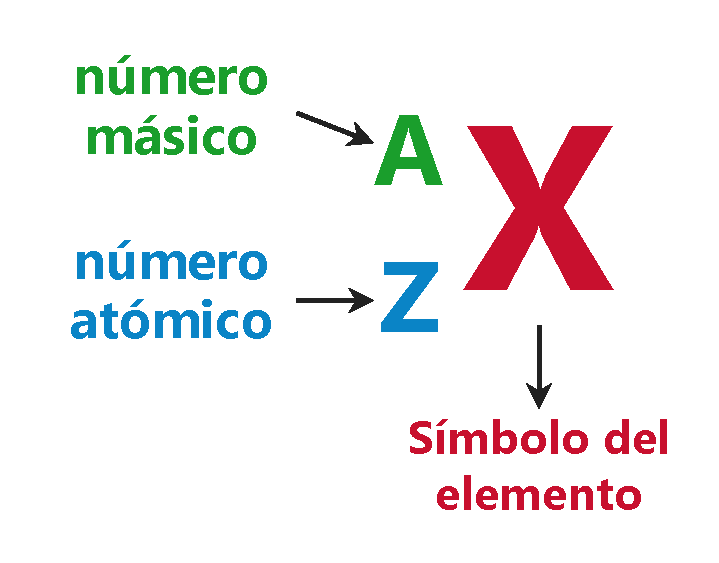
\includegraphics[width=0.8\linewidth]{Figuras_SVG_ES/pdf/U6_numero_masico_atomico.pdf}
        \caption{Representación del número másico y el número atómico}
        \label{fig:massatomic}
    \end{figure}
\end{minipage}
%\begin{figure}[H]
%    \centering
%    \includegraphics[scale=0.6]{images/SP_atomo/z_a_atomica_figura.pdf}
%    \caption{Representation of mass number and atomic number}
%    \label{fig:massatomic}
%\end{figure}
\begin{example}
    Vamos a determinar el número de protones, neutrones y electrones en los siguientes átomos neutros:
    \begin{itemize}
        \item \textbf{\isotope{Na} (Sodio):}
        \begin{itemize}
            \item Protones: \( Z = 11 \) → 11 protones
            \item Electrones: Al ser neutro, 11 electrones
            \item Neutrones: \( \ntr = A - Z = 23 - 11 = 12 \) neutrones
        \end{itemize}

        \item \textbf{\isotope{Po} (Polonio):}
        \begin{itemize}
            \item Protones: \( Z = 84 \) → 84 protones
            \item Electrones: Al ser neutro, 84 electrones
            \item Neutrones: \( \ntr = A - Z = 209 - 84 = 125 \) neutrones
        \end{itemize}
    \end{itemize}
\end{example}


\begin{exercise}
    Indica el número de protones, neutrones y electrones de un átomo de cloro \isotope{Cl}.

    \begin{solu}
        Para resolver este ejercicio, necesitamos interpretar la notación isotópica del cloro.

        A partir de la notación \isotope{Cl} obtenemos:
        \begin{itemize}
            \item Número másico (A) = 35 (parte superior)
            \item Número atómico (Z) = 17 (parte inferior)
        \end{itemize}

        \textbf{Paso 1: Calcular el número de protones}

        El número atómico (Z) indica directamente el número de protones:
        \[
            \text{Número de protones} = Z = 17
        \]

        \textbf{Paso 2: Calcular el número de neutrones}

        El número de neutrones se calcula restando el número atómico del número másico:
        \[
            \text{Número de neutrones} = A - Z = 35 - 17 = 18
        \]

        \textbf{Paso 3: Calcular el número de electrones}

        Dado que el ejercicio indica que se trata de un átomo (no un ion), es eléctricamente neutro. Por tanto, el número de electrones es igual al número de protones:
        \[
            \text{Número de electrones} = Z = 17
        \]

        \textbf{Respuesta:} El átomo de cloro-35 tiene \textbf{17 protones, 18 neutrones y 17 electrones}.
    \end{solu}
\end{exercise}
\begin{exercise}
    ¿Cómo representarías un átomo de potasio eléctricamente neutro si Z = 19 y A = 39? ¿Cuántos protones, neutrones y electrones tiene?
    \begin{solu}
        \textbf{Paso 1: Representación del átomo}

        Para representar un átomo utilizamos la notación \ch{^{A}_{Z}X}, donde:
        \begin{itemize}
            \item X = símbolo del elemento (K para potasio)
            \item A = número másico = 39
            \item Z = número atómico = 19
        \end{itemize}

        Por tanto, la representación es: \ch{^{39}_{19}K}

        \textbf{Paso 2: Calcular el número de protones}

        El número de protones es igual al número atómico:
        \[
            \text{Número de protones} = Z = 19
        \]

        \textbf{Paso 3: Calcular el número de neutrones}

        El número de neutrones se obtiene restando:
        \[
            \text{Número de neutrones} = A - Z = 39 - 19 = 20
        \]

        \textbf{Paso 4: Calcular el número de electrones}

        Dado que el átomo es eléctricamente neutro (no tiene carga), el número de electrones es igual al número de protones:
        \[
            \text{Número de electrones} = 19
        \]

        \textbf{Respuesta:} El átomo se representa como \ch{^{39}_{19}K} y tiene \textbf{19 protones, 20 neutrones y 19 electrones}.
    \end{solu}
\end{exercise}

\begin{exercise}
    ¿Podemos afirmar que Z siempre indica el número de electrones? Explica tu respuesta.
    \begin{solu}
        \textbf{Análisis del concepto:}

        El número atómico (Z) es una propiedad que define el elemento químico y representa el número de protones en el núcleo del átomo. Este valor es constante para cada elemento.

        \textbf{Caso 1: Átomo neutro}

        En un átomo eléctricamente neutro, la carga positiva de los protones debe estar exactamente compensada por la carga negativa de los electrones. Por tanto:
        \[
            \text{Número de electrones} = \text{Número de protones} = Z
        \]

        En este caso, \textbf{sí} podemos decir que Z indica el número de electrones.

        \textbf{Caso 2: Iones (átomos cargados)}

        Cuando un átomo gana o pierde electrones, se convierte en un ion:
        \begin{itemize}
            \item \textbf{Catión} (carga positiva): ha perdido electrones
            \[
                \text{Número de electrones} = Z - \text{carga positiva}
            \]
            Ejemplo: \ch{Na^{+}} tiene Z = 11, pero solo 10 electrones.

            \item \textbf{Anión} (carga negativa): ha ganado electrones
            \[
                \text{Número de electrones} = Z + \text{carga negativa}
            \]
            Ejemplo: \ch{Cl^{-}} tiene Z = 17, pero 18 electrones.
        \end{itemize}

        En estos casos, Z \textbf{no} indica el número de electrones.

        \textbf{Respuesta:} No siempre. Z indica el número de protones, que es igual al número de electrones SOLO si el átomo es neutro. Si el átomo tiene carga (es un ion), el número de electrones será diferente del valor de Z.
    \end{solu}
\end{exercise}
\begin{exercise}
    El número de neutrones del litio es una unidad más que el número de protones. Sabiendo que su número másico es 7:
    \begin{enumerate}[label=\letraminuscula]
    \item ¿Cuál es su número atómico?
    \item ¿Cuántos electrones tiene un átomo de litio eléctricamente neutro?
    \end{enumerate}
    \begin{solu}
        \textbf{Datos:}
        \begin{itemize}
            \item Número másico: A = 7
            \item Relación: número de neutrones = número de protones + 1
        \end{itemize}

        \textbf{Apartado a) Calcular el número atómico}

        \textbf{Paso 1:} Expresar la relación entre neutrones y protones

        Si llamamos Z al número de protones:
        \[
            \text{Número de neutrones} = Z + 1
        \]

        \textbf{Paso 2:} Utilizar la relación del número másico

        Sabemos que el número másico es la suma de protones y neutrones:
        \[
            A = \text{protones} + \text{neutrones}
        \]
        \[
            7 = Z + (Z + 1)
        \]

        \textbf{Paso 3:} Resolver la ecuación
        \[
            7 = 2Z + 1
        \]
        \[
            6 = 2Z
        \]
        \[
            Z = 3
        \]

        \textbf{Respuesta a):} El número atómico del litio es \textbf{Z = 3}.

        \textbf{Apartado b) Calcular el número de electrones}

        Dado que el ejercicio indica que el átomo es eléctricamente neutro, el número de electrones debe ser igual al número de protones para que las cargas se compensen:
        \[
            \text{Número de electrones} = Z = 3
        \]

        \textbf{Respuesta b):} Un átomo de litio eléctricamente neutro tiene \textbf{3 electrones}.

        \textbf{Verificación:}
        \begin{itemize}
            \item Protones: 3
            \item Neutrones: 3 + 1 = 4
            \item Número másico: 3 + 4 = 7 \( \checkmark \)
        \end{itemize}
    \end{solu}
\end{exercise}
\begin{exercise}
    Representa mediante la notación \ch{^{A}_{Z}X} indicando el número de protones, neutrones y electrones de los siguientes átomos:
    \begin{multicols}{2}
        \begin{enumerate}[label=\letraminuscula]
    \item Boro con 5 protones y 6 neutrones
    \item Nitrógeno con 7 protones y 7 neutrones
    \item Carbono con 6 protones y 6 neutrones
    \item Oxígeno con 8 protones y 8 neutrones
    \item Flúor con 9 protones y 10 neutrones
    \item Helio con 2 protones y 2 neutrones
        \end{enumerate}
    \end{multicols}
    \begin{solu}
        Para cada átomo seguiremos estos pasos:
        \begin{enumerate}
            \item Identificar Z (número de protones)
            \item Calcular A (número másico = protones + neutrones)
            \item Determinar el símbolo del elemento
            \item Calcular los electrones (igual a los protones si el átomo es neutro)
        \end{enumerate}

        \textbf{a) Boro con 5 protones y 6 neutrones}
        \begin{itemize}
            \item Z = 5 (protones)
            \item A = 5 + 6 = 11
            \item Símbolo: B
            \item Electrones = 5 (átomo neutro)
        \end{itemize}
        Representación: \ch{^{11}_{5}B}

        \textbf{Respuesta:} \ch{^{11}_{5}B} tiene 5 protones, 6 neutrones y 5 electrones.

        \textbf{b) Nitrógeno con 7 protones y 7 neutrones}
        \begin{itemize}
            \item Z = 7 (protones)
            \item A = 7 + 7 = 14
            \item Símbolo: N
            \item Electrones = 7 (átomo neutro)
        \end{itemize}
        Representación: \ch{^{14}_{7}N}

        \textbf{Respuesta:} \ch{^{14}_{7}N} tiene 7 protones, 7 neutrones y 7 electrones.

        \textbf{c) Carbono con 6 protones y 6 neutrones}
        \begin{itemize}
            \item Z = 6 (protones)
            \item A = 6 + 6 = 12
            \item Símbolo: C
            \item Electrones = 6 (átomo neutro)
        \end{itemize}
        Representación: \ch{^{12}_{6}C}

        \textbf{Respuesta:} \ch{^{12}_{6}C} tiene 6 protones, 6 neutrones y 6 electrones.

        \textbf{d) Oxígeno con 8 protones y 8 neutrones}
        \begin{itemize}
            \item Z = 8 (protones)
            \item A = 8 + 8 = 16
            \item Símbolo: O
            \item Electrones = 8 (átomo neutro)
        \end{itemize}
        Representación: \ch{^{16}_{8}O}

        \textbf{Respuesta:} \ch{^{16}_{8}O} tiene 8 protones, 8 neutrones y 8 electrones.

        \textbf{e) Flúor con 9 protones y 10 neutrones}
        \begin{itemize}
            \item Z = 9 (protones)
            \item A = 9 + 10 = 19
            \item Símbolo: F
            \item Electrones = 9 (átomo neutro)
        \end{itemize}
        Representación: \ch{^{19}_{9}F}

        \textbf{Respuesta:} \ch{^{19}_{9}F} tiene 9 protones, 10 neutrones y 9 electrones.

        \textbf{f) Helio con 2 protones y 2 neutrones}
        \begin{itemize}
            \item Z = 2 (protones)
            \item A = 2 + 2 = 4
            \item Símbolo: He
            \item Electrones = 2 (átomo neutro)
        \end{itemize}
        Representación: \ch{^{4}_{2}He}

        \textbf{Respuesta:} \ch{^{4}_{2}He} tiene 2 protones, 2 neutrones y 2 electrones.
    \end{solu}
\end{exercise}
\begin{exercise}
    Indica el número de protones, neutrones y electrones de los siguientes átomos:
    \begin{multicols}{5}
        \begin{enumerate}[label=\letraminuscula]
        \item \isotope{He}
        \item \isotope{F}
        \item \isotope{Ne}
        \item \isotope{Mg}
        \item \isotope{Ar}
        \end{enumerate}
    \end{multicols}
    \begin{solu}
        Para resolver este ejercicio, interpretaremos la notación isotópica de cada átomo y aplicaremos las siguientes fórmulas:
        \begin{itemize}
            \item Número de protones = Z (número atómico, parte inferior)
            \item Número de neutrones = A - Z (número másico - número atómico)
            \item Número de electrones = Z (si el átomo es neutro)
        \end{itemize}

        \textbf{a) \isotope{He}}
        \begin{itemize}
            \item Z = 2 (número atómico)
            \item A = 4 (número másico)
            \item Protones = 2
            \item Neutrones = 4 - 2 = 2
            \item Electrones = 2 (átomo neutro)
        \end{itemize}
        \textbf{Respuesta:} 2 protones, 2 neutrones, 2 electrones.

        \textbf{b) \isotope{F}}
        \begin{itemize}
            \item Z = 9 (número atómico)
            \item A = 19 (número másico)
            \item Protones = 9
            \item Neutrones = 19 - 9 = 10
            \item Electrones = 9 (átomo neutro)
        \end{itemize}
        \textbf{Respuesta:} 9 protones, 10 neutrones, 9 electrones.

        \textbf{c) \isotope{Ne}}
        \begin{itemize}
            \item Z = 10 (número atómico)
            \item A = 20 (número másico)
            \item Protones = 10
            \item Neutrones = 20 - 10 = 10
            \item Electrones = 10 (átomo neutro)
        \end{itemize}
        \textbf{Respuesta:} 10 protones, 10 neutrones, 10 electrones.

        \textbf{d) \isotope{Mg}}
        \begin{itemize}
            \item Z = 12 (número atómico)
            \item A = 24 (número másico)
            \item Protones = 12
            \item Neutrones = 24 - 12 = 12
            \item Electrones = 12 (átomo neutro)
        \end{itemize}
        \textbf{Respuesta:} 12 protones, 12 neutrones, 12 electrones.

        \textbf{e) \isotope{Ar}}
        \begin{itemize}
            \item Z = 18 (número atómico)
            \item A = 40 (número másico)
            \item Protones = 18
            \item Neutrones = 40 - 18 = 22
            \item Electrones = 18 (átomo neutro)
        \end{itemize}
        \textbf{Respuesta:} 18 protones, 22 neutrones, 18 electrones.

        \textbf{f) \isotope{Ca}}
        \begin{itemize}
            \item Z = 20 (número atómico)
            \item A = 40 (número másico)
            \item Protones = 20
            \item Neutrones = 40 - 20 = 20
            \item Electrones = 20 (átomo neutro)
        \end{itemize}
        \textbf{Respuesta:} 20 protones, 20 neutrones, 20 electrones.
    \end{solu}
\end{exercise}
\section{Iones}
\begin{definition}[ion]
    Es un átomo (o grupo de átomos) que ha ganado o perdido electrones y por tanto tiene una carga eléctrica.
\end{definition}
Cuando un átomo gana o pierde electrones, deja de ser neutro y se convierte en un ion:
\begin{itemize}
    \item \negsubro{Catión} (\textbf{ion positivo}): Se forma cuando un átomo \textbf{pierde electrones}. Al tener menos electrones que protones, queda con carga positiva. Se representa con el signo \( + \).

    Ejemplo: \ch{Na^{+}} (el sodio ha perdido 1 electrón)

    \item \negsubro{Anión} (\textbf{ion negativo}): Se forma cuando un átomo \textbf{gana electrones}. Al tener más electrones que protones, queda con carga negativa. Se representa con el signo \( - \).

    Ejemplo: \ch{Cl^{-}} (el cloro ha ganado 1 electrón)
\end{itemize}
\begin{remark}
    \textbf{Regla importante:} El número de protones (Z) \textbf{nunca cambia} cuando se forma un ion, porque los protones están en el núcleo y no se pueden ganar o perder fácilmente. Solo cambia el número de electrones.
\end{remark}
\begin{example}
    Vamos a determinar el número de protones, neutrones y electrones en los siguientes iones:

    \begin{itemize}
        \item \textbf{\isotope{23,11,Na}$^{+}$ (Catión sodio):}
        \begin{itemize}
            \item Protones: \( Z = 11 \) → 11 protones (no cambia)
            \item Neutrones: \( A - Z = 23 - 11 = 12 \) neutrones
            \item Electrones: 10 electrones (ha perdido 1 electrón: 11 - 1 = 10)
        \end{itemize}

        \item \textbf{\isotope{35,17,Cl}$^{-}$ (Anión cloro):}
        \begin{itemize}
            \item Protones: \( Z = 17 \) → 17 protones (no cambia)
            \item Neutrones: \( A - Z = 35 - 17 = 18 \) neutrones
            \item Electrones: 18 electrones (ha ganado 1 electrón: 17 + 1 = 18)
        \end{itemize}
    \end{itemize}
\end{example}
\begin{exercise}
    Indica el número de protones, neutrones y electrones de los siguientes iones:
    \begin{multicols}{4}
        \begin{enumerate}[label=\letraminuscula]
        \item \isotope{Ca}$^{2+}$
        \item \isotope{O}$^{2-}$
        \item \isotope{Al}$^{3+}$
        \item \isotope{S}$^{2-}$
        \end{enumerate}
    \end{multicols}
    \begin{solu}
        Para resolver este ejercicio, debemos recordar que:
        \begin{itemize}
            \item El número de protones es siempre igual a Z (número atómico) y no cambia.
            \item El número de neutrones = A - Z
            \item Para los iones:
            \begin{itemize}
                \item Cationes (carga positiva): han perdido electrones → electrones = Z - carga
                \item Aniones (carga negativa): han ganado electrones → electrones = Z + carga
            \end{itemize}
        \end{itemize}

        \textbf{a) \isotope{Ca}$^{2+}$}

        \textbf{Paso 1:} Identificar los datos a partir de la notación isotópica
        \begin{itemize}
            \item Z = 20 (número atómico del calcio)
            \item A = 40 (número másico)
            \item Carga = 2+ (catión)
        \end{itemize}

        \textbf{Paso 2:} Calcular los protones
        \[
            \text{Protones} = Z = 20
        \]

        \textbf{Paso 3:} Calcular los neutrones
        \[
            \text{Neutrones} = A - Z = 40 - 20 = 20
        \]

        \textbf{Paso 4:} Calcular los electrones

        Al ser un catión con carga 2+, ha perdido 2 electrones:
        \[
            \text{Electrones} = Z - 2 = 20 - 2 = 18
        \]

        \textbf{Respuesta:} 20 protones, 20 neutrones, 18 electrones.

        \textbf{b) \isotope{O}$^{2-}$}

        \textbf{Paso 1:} Identificar los datos a partir de la notación isotópica
        \begin{itemize}
            \item Z = 8 (número atómico del oxígeno)
            \item A = 16 (número másico)
            \item Carga = 2- (anión)
        \end{itemize}

        \textbf{Paso 2:} Calcular los protones
        \[
            \text{Protones} = Z = 8
        \]

        \textbf{Paso 3:} Calcular los neutrones
        \[
            \text{Neutrones} = A - Z = 16 - 8 = 8
        \]

        \textbf{Paso 4:} Calcular los electrones

        Al ser un anión con carga 2-, ha ganado 2 electrones:
        \[
            \text{Electrones} = Z + 2 = 8 + 2 = 10
        \]

        \textbf{Respuesta:} 8 protones, 8 neutrones, 10 electrones.

        \textbf{c) \isotope{Al}$^{3+}$}

        \textbf{Paso 1:} Identificar los datos a partir de la notación isotópica
        \begin{itemize}
            \item Z = 13 (número atómico del aluminio)
            \item A = 27 (número másico)
            \item Carga = 3+ (catión)
        \end{itemize}

        \textbf{Paso 2:} Calcular los protones
        \[
            \text{Protones} = Z = 13
        \]

        \textbf{Paso 3:} Calcular los neutrones
        \[
            \text{Neutrones} = A - Z = 27 - 13 = 14
        \]

        \textbf{Paso 4:} Calcular los electrones

        Al ser un catión con carga 3+, ha perdido 3 electrones:
        \[
            \text{Electrones} = Z - 3 = 13 - 3 = 10
        \]

        \textbf{Respuesta:} 13 protones, 14 neutrones, 10 electrones.

        \textbf{d) \isotope{S}$^{2-}$}

        \textbf{Paso 1:} Identificar los datos a partir de la notación isotópica
        \begin{itemize}
            \item Z = 16 (número atómico del azufre)
            \item A = 32 (número másico)
            \item Carga = 2- (anión)
        \end{itemize}

        \textbf{Paso 2:} Calcular los protones
        \[
            \text{Protones} = Z = 16
        \]

        \textbf{Paso 3:} Calcular los neutrones
        \[
            \text{Neutrones} = A - Z = 32 - 16 = 16
        \]

        \textbf{Paso 4:} Calcular los electrones

        Al ser un anión con carga 2-, ha ganado 2 electrones:
        \[
            \text{Electrones} = Z + 2 = 16 + 2 = 18
        \]

        \textbf{Respuesta:} 16 protones, 16 neutrones, 18 electrones.
    \end{solu}
\end{exercise}
\begin{exercise}
    ¿Cuántos electrones ha perdido o ganado un átomo de aluminio (\( Z = 13 \)) para convertirse en \ch{Al^{3+}}?
    \begin{solu}
        \textbf{Datos:}
        \begin{itemize}
            \item Número atómico del aluminio: Z = 13
            \item Ion formado: \ch{Al^{3+}}
            \item Carga del ion: 3+
        \end{itemize}

        \textbf{Paso 1:} Determinar el número de electrones en el átomo neutro

        Un átomo de aluminio eléctricamente neutro tiene el mismo número de electrones que de protones:
        \[
            \text{Electrones en el átomo neutro} = Z = 13
        \]

        \textbf{Paso 2:} Determinar el número de electrones en el ion

        El ion \ch{Al^{3+}} tiene una carga positiva de 3+, lo que significa que:
        \[
            \text{Electrones en el ion} = Z - 3 = 13 - 3 = 10
        \]

        \textbf{Paso 3:} Calcular cuántos electrones se han perdido o ganado

        Comparamos el número de electrones antes y después:
        \[
            \text{Electrones perdidos} = 13 - 10 = 3
        \]

        \textbf{Análisis del resultado:}

        Dado que la carga es positiva (3+), esto indica una pérdida de electrones, no una ganancia. El átomo de aluminio ha cedido 3 electrones para formar el catión \ch{Al^{3+}}.

        \textbf{Verificación:}
        \begin{itemize}
            \item Átomo neutro: 13 protones (+) y 13 electrones (-) → carga neta = 0
            \item Ion \ch{Al^{3+}}: 13 protones (+) y 10 electrones (-) → carga neta = +3 \( \checkmark \)
        \end{itemize}

        \textbf{Respuesta:} El átomo de aluminio ha \textbf{perdido 3 electrones} para convertirse en \ch{Al^{3+}}.
    \end{solu}
\end{exercise}
\section{Isótopos}
\begin{definition}[isótopos]
    Son átomos del mismo elemento químico (tienen el mismo número atómico \( Z \)) pero diferente número de neutrones y por tanto diferente número másico (\( A \)).
\end{definition}
\textbf{Características de los isótopos:}
\begin{itemize}
    \item Tienen el \textbf{mismo número de protones} (mismo \( Z \))
    \item Tienen \textbf{diferente número de neutrones}
    \item Tienen \textbf{diferente número másico} (\( A \))
    \item Son del \textbf{mismo elemento químico}
    \item Tienen \textbf{propiedades químicas muy similares}
\end{itemize}
\begin{example}
    El carbono tiene varios isótopos. Los más comunes son:
    \begin{itemize}
        \item \textbf{Carbono-12:} \isotope{C}
        \begin{itemize}
            \item 6 protones, 6 neutrones, 6 electrones
            \item Es el isótopo más abundante (98,9\%)
        \end{itemize}

        \item \textbf{Carbono-13:} \isotope{13,C}
        \begin{itemize}
            \item 6 protones, 7 neutrones, 6 electrones
            \item Menos abundante (1,1\%)
        \end{itemize}
        \item \textbf{Carbono-14:} \isotope{14,C}
        \begin{itemize}
            \item 6 protones, 8 neutrones, 6 electrones
            \item Es radiactivo y se utiliza para datar fósiles
        \end{itemize}
    \end{itemize}
    Los tres son carbono porque tienen 6 protones, pero se diferencian en el número de neutrones.
\end{example}
%\begin{remark}
%    \textbf{Practical application:} Carbon-14 is used to determine the age of archaeological remains and fossils. This method is called ``carbon-14 dating'' and has made it possible to determine the age of mummies, ancient scrolls, and prehistoric remains.
%\end{remark}
\begin{exercise}
    ¿Cuáles de los siguientes átomos son isótopos entre sí?
    \begin{multicols}{4}
        \begin{enumerate}[label=\letraminuscula]
        \item \isotope{Ne}
        \item \isotope{21,Ne}
        \item \isotope{F}
        \item \isotope{Na}
        \end{enumerate}
    \end{multicols}
    \begin{solu}
        \textbf{Concepto de isótopos:}

        Los isótopos son átomos del mismo elemento (mismo número atómico Z) que tienen diferente número de neutrones y por tanto diferente número másico (A).

        \textbf{Condición para ser isótopos:}
        \[
            \text{Mismo Z (número atómico)} \quad \text{y} \quad \text{Diferente A (número másico)}
        \]

        \textbf{Paso 1:} Analizar cada átomo e identificar Z y A

        \textbf{a) \isotope{Ne}}
        \begin{itemize}
            \item Elemento: Neón (Ne)
            \item Z = 10 (número atómico)
            \item A = 20 (número másico)
        \end{itemize}

        \textbf{b) \isotope{Ne}}
        \begin{itemize}
            \item Elemento: Neón (Ne)
            \item Z = 10 (número atómico)
            \item A = 22 (número másico)
        \end{itemize}

        \textbf{c) \isotope{F}}
        \begin{itemize}
            \item Elemento: Flúor (F)
            \item Z = 9 (número atómico)
            \item A = 19 (número másico)
        \end{itemize}

        \textbf{d) \isotope{Na}}
        \begin{itemize}
            \item Elemento: Sodio (Na)
            \item Z = 11 (número atómico)
            \item A = 23 (número másico)
        \end{itemize}

        \textbf{Paso 2:} Comparar los átomos para identificar los isótopos

        Organizamos los datos en una tabla:

        \begin{center}
            % --- tabla antigua ---
            % \begin{tabular}{|c|c|c|c|}
                % \hline
                % \textbf{Átomo} & \textbf{Elemento} & \textbf{Z} & \textbf{A} \\
                % \hline
                % a)            & Ne               & 10         & 20         \\
                % \hline
                % b)            & Ne               & 10         & 22         \\
                % \hline
                % c)            & F                & 9          & 19         \\
                % \hline
                % d)            & Na               & 11         & 23         \\
                % \hline
            % \end{tabular}
            % --- tabla nueva ---
            \begin{tabular}{@{}cccc@{}}
                \toprule
                \textbf{Átomo} & \textbf{Elemento} & \textbf{Z} & \textbf{A} \\
                \midrule
                a) & Ne & 10 & 20 \\[3pt]
                b) & Ne & 10 & 22 \\[3pt]
                c) & F & 9 & 19 \\[3pt]
                d) & Na & 11 & 23 \\
                \bottomrule
            \end{tabular}
        \end{center}

        \textbf{Paso 3:} Identificar los isótopos

        Buscamos átomos con el mismo Z pero diferente A:
        \begin{itemize}
            \item Los átomos \textbf{a)} y \textbf{b)} son ambos neón (Z = 10)
            \item Tienen diferente número másico: A = 20 y A = 22
            \item Por tanto, \textbf{cumplen la condición para ser isótopos}
        \end{itemize}

        Los átomos c) y d) son elementos diferentes (F y Na), por lo que no pueden ser isótopos entre sí ni de los anteriores.

        \textbf{Verificación adicional:}

        Para \isotope{Ne}:
        \begin{itemize}
            \item Protones = 10
            \item Neutrones = 20 - 10 = 10
        \end{itemize}

        Para \isotope{Ne}:
        \begin{itemize}
            \item Protones = 10
            \item Neutrones = 22 - 10 = 12
        \end{itemize}

        Mismo número de protones pero diferente número de neutrones. \( \checkmark \)

        \textbf{Respuesta:} Los átomos \textbf{a) y b)} son isótopos entre sí. Se trata de dos isótopos del neón: neón-20 y neón-22.
    \end{solu}
\end{exercise}

\begin{exercise}
    El hidrógeno tiene tres isótopos conocidos:
    \begin{itemize}
        \item Hidrógeno común: 1 protón, 0 neutrones
        \item Deuterio: 1 protón, 1 neutrón
        \item Tritio: 1 protón, 2 neutrones
    \end{itemize}
    Represéntalos utilizando la notación \ch{^{A}_{Z}X}.
    \begin{solu}
        Para representar cada isótopo, necesitamos calcular:
        \begin{itemize}
            \item Z = número de protones (siempre el mismo para los tres isótopos)
            \item A = número másico = protones + neutrones
            \item X = símbolo del elemento (H para hidrógeno)
        \end{itemize}

        \textbf{Isótopo 1: Hidrógeno común (Protio)}

        \textbf{Paso 1:} Identificar los datos
        \begin{itemize}
            \item Número de protones = 1
            \item Número de neutrones = 0
        \end{itemize}

        \textbf{Paso 2:} Calcular Z y A
        \[
            Z = \text{número de protones} = 1
        \]
        \[
            A = \text{protones} + \text{neutrones} = 1 + 0 = 1
        \]

        \textbf{Paso 3:} Representar con la notación
        \[
            \boxed{\ch{^{1}_{1}H}}
        \]

        \textbf{Isótopo 2: Deuterio}

        \textbf{Paso 1:} Identificar los datos
        \begin{itemize}
            \item Número de protones = 1
            \item Número de neutrones = 1
        \end{itemize}

        \textbf{Paso 2:} Calcular Z y A
        \[
            Z = \text{número de protones} = 1
        \]
        \[
            A = \text{protones} + \text{neutrones} = 1 + 1 = 2
        \]

        \textbf{Paso 3:} Representar con la notación
        \[
            \boxed{\ch{^{2}_{1}H}} \quad \text{(también representado como \ch{^{2}_{1}D})}
        \]

        \textbf{Isótopo 3: Tritio}

        \textbf{Paso 1:} Identificar los datos
        \begin{itemize}
            \item Número de protones = 1
            \item Número de neutrones = 2
        \end{itemize}

        \textbf{Paso 2:} Calcular Z y A
        \[
            Z = \text{número de protones} = 1
        \]
        \[
            A = \text{protones} + \text{neutrones} = 1 + 2 = 3
        \]

        \textbf{Paso 3:} Representar con la notación
        \[
            \boxed{\ch{^{3}_{1}H}} \quad \text{(también representado como \ch{^{3}_{1}T})}
        \]

        \textbf{Verificación de que son isótopos:}

        Los tres átomos cumplen la condición para ser isótopos:
        \begin{itemize}
            \item Mismo número atómico: Z = 1 (todos son hidrógeno) \( \checkmark \)
            \item Diferente número másico: A = 1, 2 y 3 respectivamente \( \checkmark \)
            \item Diferente número de neutrones: 0, 1 y 2 respectivamente \( \checkmark \)
        \end{itemize}

        \textbf{Respuesta:}
        \begin{itemize}
            \item Hidrógeno común (Protio): \ch{^{1}_{1}H}
            \item Deuterio: \ch{^{2}_{1}H} o \ch{^{2}_{1}D}
            \item Tritio: \ch{^{3}_{1}H} o \ch{^{3}_{1}T}
        \end{itemize}

        \textbf{Nota:} El deuterio y el tritio son tan importantes que tienen sus propios símbolos (D y T), aunque lo más habitual es usar H para todos los isótopos del hidrógeno.
    \end{solu}
\end{exercise}

\section{Configuración Electrónica}
Ya sabemos que los electrones se distribuyen alrededor del núcleo en diferentes niveles de energía, pero no lo hacen al azar. Los electrones se organizan en diferentes zonas o ``pisos'' alrededor del núcleo.
\begin{definition}{Configuración electrónica}
    La \textbf{configuración electrónica} es como la ``dirección postal'' de los electrones. Nos indica exactamente dónde está cada electrón dentro del átomo, mediante una serie de números y letras.
\end{definition}
\newpage

\subsection{Niveles de energía: las capas del átomo}
\begin{minipage}{0.45\textwidth}
    Imagina el átomo como un edificio de apartamentos donde el núcleo está en el centro y los electrones viven en diferentes pisos alrededor de él:
    \begin{itemize}
        \item Los electrones más cercanos al núcleo (piso 1) están más fuertemente atraídos hacia él
        \item Los electrones más alejados (pisos superiores) están menos atraídos
        \item Cada piso se llama \textbf{nivel de energía} y se numera del 1 al 7
    \end{itemize}
    \begin{remark}
        \textbf{Analogía útil:} Los niveles de energía son como las capas de una cebolla. La primera capa (la más interna) es el nivel 1, la segunda capa es el nivel 2, y así sucesivamente hasta un máximo de 7 capas.
    \end{remark}
\end{minipage}
\hfill
\begin{minipage}{0.45\textwidth}
    \begin{figure}[H]
        \centering
        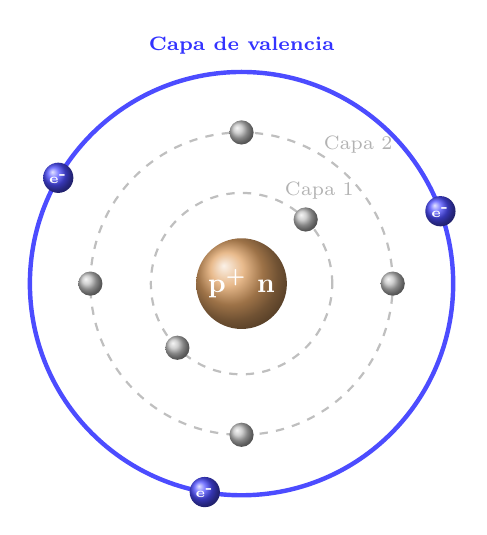
\begin{tikzpicture}[scale=0.48]
            % Núcleo con degradado ocre (solo p+ y n)
            \shade[ball color=orange!80!black!60] (0,0) circle (1.2cm);
            \node[font=\normalsize\bfseries, white] at (0,0) {p\textsuperscript{+} n};
            % Capa 1 (radio 2.4)
            \draw[gray!50, thick, dashed] (0,0) circle (2.4cm);
            % Etiqueta Capa 1: entre capa 1 (2.4) y capa 2 (4.0), a radio ~3.2
            \node[gray!60, font=\scriptsize] at (50:3.2) {Capa 1};
            % Capa 2 (radio 4.0, más separada)
            \draw[gray!50, thick, dashed] (0,0) circle (4.0cm);
            % Etiqueta Capa 2: entre capa 2 (4.0) y valencia (5.6), a radio ~4.8
            \node[gray!60, font=\scriptsize] at (50:4.8) {Capa 2};
            % Capa de valencia (radio 5.6, resaltada)
            \draw[blue!70, ultra thick] (0,0) circle (5.6cm);
            \node[blue!80, font=\scriptsize\bfseries] at (0, 6.3) {Capa de valencia};
            % Electrones de valencia (azules)
            \foreach \angle in {20, 150, 260} {
                \shade[ball color=blue!70] (\angle:5.6) circle (0.4cm);
                \node[white, font=\tiny\bfseries] at (\angle:5.6) {e\textsuperscript{-}};
            }
            % Electrones internos capa 1 (grises)
            \foreach \angle in {45, 225} {
                \shade[ball color=gray!50] (\angle:2.4) circle (0.32cm);
            }
            % Electrones internos capa 2 (grises)
            \foreach \angle in {0, 90, 180, 270} {
                \shade[ball color=gray!50] (\angle:4.0) circle (0.32cm);
            }
        \end{tikzpicture}
        \caption{Niveles de energía y capa de valencia.}
        \label{fig:niveles_capa_de_valencia}
    \end{figure}
\end{minipage}

\subsection{Orbitales: las habitaciones dentro de cada piso}
Dentro de cada nivel (cada piso), hay diferentes tipos de "habitaciones" donde pueden estar los electrones. Estas habitaciones se llaman \textbf{subniveles} u \textbf{orbitales} y se representan con letras: \textbf{s, p, d, f}
\begin{itemize}
    \item \textbf{Subnivel s}: El más sencillo, puede contener hasta \textbf{2 electrones} como máximo
    \item \textbf{Subnivel p}: Ligeramente más grande, puede contener hasta \textbf{6 electrones} como máximo
    \item \textbf{Subnivel d}: Más amplio, puede contener hasta \textbf{10 electrones} como máximo
    \item \textbf{Subnivel f}: El más grande, puede contener hasta \textbf{14 electrones} como máximo
\end{itemize}
\subsection{¿Qué orbitales hay en cada nivel?}
No todos los niveles tienen todos los tipos de orbitales. Aquí tienes la lista completa:
\begin{itemize}
    \item \textbf{Nivel 1}: solo tiene el orbital \textbf{s} → escribimos \( 1s \)
    \item \textbf{Nivel 2}: tiene los orbitales \textbf{s} y \textbf{p} → escribimos \( 2s, 2p \)
    \item \textbf{Nivel 3}: tiene \textbf{s, p} y \textbf{d} → escribimos \( 3s, 3p, 3d \)
    \item \textbf{Nivel 4}: tiene \textbf{s, p, d} y \textbf{f} → escribimos \( 4s, 4p, 4d, 4f \)
    \item \textbf{Niveles 5, 6 y 7}: igual que el nivel 4, tienen s, p, d y f
\end{itemize}
\begin{remark}
    \textbf{Patrón observable:} Cada nuevo nivel añade un tipo más de orbital. El nivel 1 solo tiene s, el nivel 2 añade p, el nivel 3 añade d, y el nivel 4 añade f.
\end{remark}
\subsection{Cómo se escriben los orbitales}
Cuando escribimos un orbital, utilizamos:
\begin{enumerate}
    \item Un \textbf{número} que indica el nivel (1, 2, 3, 4...)
    \item Una \textbf{letra} que indica el tipo de orbital (s, p, d, f)
    \item Un \textbf{exponente} (número pequeño arriba) que indica cuántos electrones hay en ese orbital
\end{enumerate}
\textbf{Ejemplos:}
\begin{itemize}
    \item \( 1s^2 \) → En el nivel 1, orbital s, hay 2 electrones
    \item \( 2p^6 \) → En el nivel 2, orbital p, hay 6 electrones
    \item \( 3d^{10} \) → En el nivel 3, orbital d, hay 10 electrones
    \item \( 3s^1 \) → En el nivel 3, orbital s, hay 1 electrón
\end{itemize}
\subsection{El Diagrama de Moeller: la guía para rellenar los orbitales}
Los electrones no rellenan los orbitales en el orden que podríamos pensar (primero 1s, luego 2s, luego 2p...). Existe un orden especial que debemos seguir, y para ello usamos el \textbf{Diagrama de Moeller}.
\begin{figure}[H]
    \centering
    \begin{tikzpicture}[>=stealth, font=\sffamily\LARGE\bfseries]

        % --- Configuración de Colores ---
        \definecolor{mygreen}{RGB}{0, 128, 0}
        \definecolor{myblue}{RGB}{91, 155, 213}

        % --- Dibujado de los Subniveles ---
        % Separación horizontal (2.2) y vertical (1.2) para que las diagonales sean perfectas
        \newcommand{\subnivel}[5]{
            \node (n#3#4) at (#1*2.2, -#2*1.2) {#3\textcolor{mygreen}{\textit{#4}}\textsuperscript{\textcolor{red}{#5}}};
        }

        % Columna s (x=0)
        \foreach \n in {1,...,7} \subnivel{0}{\n}{\n}{s}{2};
        % Columna p (x=1)
        \foreach \n in {2,...,7} \subnivel{1}{\n}{\n}{p}{6};
        % Columna d (x=2)
        \foreach \n in {3,...,7} \subnivel{2}{\n}{\n}{d}{10};
        % Columna f (x=3)
        \foreach \n in {4,...,7} \subnivel{3}{\n}{\n}{f}{14};

        % --- Dibujado de las Flechas Diagonales ---
        % Estilo: pasan por el centro, color azul, y se extienden 0.8cm hacia atrás y 1cm hacia adelante
        \tikzset{flecha/.style={myblue, very thick, *->, shorten <=-0.8cm, shorten >=-1cm}}

        % Para flechas que cruzan varios nodos (del centro del primero al centro del último)
        \draw[flecha] ($(n2p.center)+(1.5,0.7)$) -- (n3s.center);
        \draw[flecha] ($(n3p.center)+(1.5,0.7)$) -- (n4s.center);
        \draw[flecha] ($(n3d.center)+(1.5,0.7)$) -- (n5s.center);
        \draw[flecha] ($(n4d.center)+(1.5,0.7)$) -- (n6s.center);
        \draw[flecha] ($(n4f.center)+(1.5,0.7)$) -- (n7s.center);
        \draw[flecha] ($(n5f.center)+(1.5,0.7)$) -- (n7p.center);
        \draw[flecha] ($(n6f.center)+(1.5,0.7)$) -- (n7d.center);

        % Para las flechas de un solo nodo (1s, 2s y 7f), definimos una dirección manual
        % para que mantengan el mismo ángulo que las demás.
        \draw[flecha] ($(n1s.center)+(1.5,0.7)$) -- (n1s.center);
        \draw[flecha] ($(n2s.center)+(1.5,0.7)$) -- (n2s.center);
        \draw[flecha] (n7f.center) ++(1.5,0.8) -- (n7f.center);

    \end{tikzpicture}
    \caption{Diagrama de Moeller}
    \label{fig:diagrama_moeller}
\end{figure}
\begin{remark}
    \textbf{Cómo usar el Diagrama de Moeller:} Cada flecha te indica qué orbitales debes recorrer. Empiezas por la primera flecha (arriba a la izquierda) y sigues el recorrido de cada flecha. El orden que se obtiene es:
    \[
        1s \rightarrow 2s \rightarrow 2p \rightarrow 3s \rightarrow 3p \rightarrow 4s \rightarrow 3d \rightarrow 4p \rightarrow ...
    \]
\end{remark}
\subsection{Cómo escribir una configuración electrónica paso a paso}
Vamos a aprender a escribir la configuración electrónica del \textbf{Sodio (Na)} que tiene \( Z = 11 \), es decir, 11 electrones.
\begin{enumerate}[label=\textbf{Paso \arabic*:}]
        \item \textbf{Identificar cuántos electrones tiene el átomo}

        El sodio tiene \( Z = 11 \), por tanto tiene \textbf{11 electrones} que debemos colocar.

        \item \textbf{Seguir el diagrama de Moeller y rellenar los orbitales en orden}

        \begin{itemize}
            \item Las flechas siempre se siguen desde el punto de partida hasta la punta de flecha, comprobando los orbitales por los que pasamos hasta llegar a la punta.

            \item Primera flecha: En este caso solo pasa por \( 1s \): Este orbital puede tener un máximo de 2 electrones. Escribimos \( 1s^2 \)

            Electrones colocados: 2. Nos quedan: 11 - 2 = 9 electrones.

            \item Segunda flecha: Tenemos la misma situación y solo pasa por \( 2s \). Este orbital puede tener un máximo de 2 electrones. Escribimos \( 2s^2 \)

            Electrones colocados: 2 (de \( 1s \)) + 2 (de \( 2s \)) = 4. Nos quedan: 11 - 4 = 7 electrones.

            \item Tercera flecha: ahora pasa por \( 2p \) y \( 3s \): Primero colocamos los electrones en el orbital \( 2p \) porque es el primero en rellenarse y como podemos colocar un máximo de \num{6} electrones entonces escribimos: \( 2p^6 \). Ahora solo nos queda 1 electrón por colocar. El siguiente orbital según la flecha será \( 3s \), en este caso podríamos poner un máximo de \num{2} electrones pero como solo nos queda \num{1} electrón por colocar entonces debemos escribir: \( 3s^1 \)

            Electrones colocados: 2 (de \( 1s \)) + 2 (de \( 2s \)) + 6 (de \( 2p \)) + 1 (de \( 3s \)) = 11. ¡Perfecto! Los hemos colocado todos

            Electrones colocados: 10 + 1 = 11.
        \end{itemize}

        \item \textbf{Escribir la configuración electrónica completa}
        \[
            \text{Configuración del Na: } 1s^2\ 2s^2\ 2p^6\ 3s^1
        \]
\end{enumerate}
\begin{remark}
    \textbf{Consejo importante:} Cuenta siempre los electrones después de cada paso para asegurarte de que no superas el número total de electrones del átomo.
\end{remark}
\begin{example}
    \textbf{Configuración electrónica del Rubidio (Rb)} con \( Z = 37 \):
    Siguiendo el diagrama de Moeller y contando 37 electrones:
    \[
        1s^2\ 2s^2\ 2p^6\ 3s^2\ 3p^6\ 4s^2\ 3d^{10}\ 4p^6\ 5s^1
    \]

    Observa que el orbital \( 3d \) se rellena \textbf{después} de \( 4s \), aunque 3 sea menor que 4. Esto es lo que indica el diagrama de Moeller.
    \textbf{Reordenado por niveles} (opcional, pero más organizado):
    \[
        1s^2\ 2s^2\ 2p^6\ 3s^2\ 3p^6\ 3d^{10}\ 4s^2\ 4p^6\ 5s^1
    \]
\end{example}
\subsection{Configuración electrónica de los iones}
Cuando un átomo se convierte en ion (gana o pierde electrones), su configuración electrónica cambia:
\begin{itemize}
    \item \textbf{Para los cationes} (iones positivos, han perdido electrones):

    Primero se escribe la configuración del átomo neutro, y después \textbf{se quitan electrones desde el final} (desde el orbital con el número más alto).

    \textbf{Ejemplo:} \ch{Na^{+}} (ha perdido 1 electrón)
    \begin{itemize}
        \item Na neutro: \( 1s^2\ 2s^2\ 2p^6\ 3s^1 \)
        \item \ch{Na^{+}}: \( 1s^2\ 2s^2\ 2p^6 \) (quitamos 1 electrón de \( 3s \))
    \end{itemize}

    \item \textbf{Para los aniones} (iones negativos, han ganado electrones):
    Primero se escribe la configuración del átomo neutro, y después \textbf{se añaden electrones} siguiendo el orden del diagrama de Moeller.

    \textbf{Ejemplo:} \ch{Cl^{-}} (ha ganado 1 electrón)
    \begin{itemize}
        \item Cl neutro (\( Z = 17 \)): \( 1s^2\ 2s^2\ 2p^6\ 3s^2\ 3p^5 \)
        \item \ch{Cl^{-}}: \( 1s^2\ 2s^2\ 2p^6\ 3s^2\ 3p^6 \) (añadimos 1 electrón a \( 3p \))
    \end{itemize}
\end{itemize}
\begin{exercise}
    Escribe la configuración electrónica del Carbono (\( Z = 6 \)) en su estado fundamental (no pierde ni gana \el{}).

    \begin{solu}
        \textbf{Datos:}
        \begin{itemize}
            \item Elemento: Carbono (C)
            \item Número atómico: Z = 6
            \item Estado: Átomo neutro (no pierde ni gana electrones)
        \end{itemize}

        \textbf{Paso 1:} Determinar el número de electrones

        Dado que el átomo está en estado fundamental y es neutro:
        \[
            \text{Número de electrones} = Z = 6
        \]

        \textbf{Paso 2:} Recordar el orden de llenado de los orbitales

        Según el principio de Aufbau, los orbitales se rellenan en orden de energía creciente:
        \[
            1s \rightarrow 2s \rightarrow 2p \rightarrow 3s \rightarrow 3p \rightarrow 4s \rightarrow 3d \rightarrow \ldots
        \]

        \textbf{Paso 3:} Aplicar las reglas de llenado

        \textbf{Regla 1 - Principio de Aufbau:} Rellenar desde el orbital de menor energía.

        \textbf{Regla 2 - Principio de exclusión de Pauli:} Cada orbital puede contener un máximo de 2 electrones con espines opuestos.

        \textbf{Regla 3 - Regla de Hund:} En orbitales de igual energía, se coloca un electrón en cada orbital antes de emparejarlos.

        \textbf{Paso 4:} Distribuir los 6 electrones

        \begin{itemize}
            \item \textbf{Orbital 1s:} Contiene 2 electrones → \(1s^2\) (quedan 4 electrones)
            \item \textbf{Orbital 2s:} Contiene 2 electrones → \(2s^2\) (quedan 2 electrones)
            \item \textbf{Orbitales 2p:} Los 2 electrones restantes van a los orbitales 2p

            El subnivel 2p tiene 3 orbitales (2p\(_x\), 2p\(_y\), 2p\(_z\)), cada uno puede contener 2 electrones (total 6).

            Según la regla de Hund, primero se coloca un electrón en cada orbital:
            \[
                2p^2 \quad (\uparrow \quad \uparrow \quad \cdot)
            \]
        \end{itemize}

        \textbf{Paso 5:} Escribir la configuración electrónica completa
        \[
            \boxed{1s^2 \, 2s^2 \, 2p^2}
        \]

        \textbf{Verificación:}
        \[
            2 + 2 + 2 = 6 \text{ electrones} \quad \checkmark
        \]

        \textbf{Respuesta:} La configuración electrónica del carbono es: \elconf{C}
    \end{solu}
\end{exercise}
\begin{exercise}
    Determina la configuración electrónica del Fósforo (\( Z = 15 \)).
    \begin{solu}
        \textbf{Datos:}
        \begin{itemize}
            \item Elemento: Fósforo (P)
            \item Número atómico: Z = 15
            \item Estado: Átomo neutro
        \end{itemize}

        \textbf{Paso 1:} Determinar el número de electrones
        \[
            \text{Número de electrones} = Z = 15
        \]

        \textbf{Paso 2:} Orden de llenado de los orbitales

        Para 15 electrones necesitamos:
        \[
            1s \rightarrow 2s \rightarrow 2p \rightarrow 3s \rightarrow 3p
        \]

        \textbf{Paso 3:} Distribuir los 15 electrones siguiendo las reglas

        \begin{itemize}
            \item \textbf{Capa n = 1:}
            \begin{itemize}
                \item \(1s^2\) → 2 electrones (quedan 13)
            \end{itemize}

            \item \textbf{Capa n = 2:}
            \begin{itemize}
                \item \(2s^2\) → 2 electrones (quedan 11)
                \item \(2p^6\) → 6 electrones (quedan 5)
            \end{itemize}

            \item \textbf{Capa n = 3:}
            \begin{itemize}
                \item \(3s^2\) → 2 electrones (quedan 3)
                \item \(3p^3\) → 3 electrones (quedan 0)

                Los 3 electrones en 3p se distribuyen según Hund:
                \[
                    3p^3 \quad (\uparrow \quad \uparrow \quad \uparrow)
                \]
                Un electrón en cada orbital antes de emparejarlos.
            \end{itemize}
        \end{itemize}

        \textbf{Paso 4:} Escribir la configuración electrónica completa
        \[
            \boxed{1s^2 \, 2s^2 \, 2p^6 \, 3s^2 \, 3p^3}
        \]

        \textbf{Verificación:}
        \[
            2 + 2 + 6 + 2 + 3 = 15 \text{ electrones} \quad \checkmark
        \]

        \textbf{Forma simplificada (configuración del núcleo interno):}

        Podemos usar el gas noble anterior (Neón, Z = 10):
        \[
            \text{P:} \quad [\text{Ne}] \, 3s^2 \, 3p^3
        \]

        \textbf{Respuesta:} La configuración electrónica del fósforo es: \elconf{P}
    \end{solu}
\end{exercise}
\begin{exercise}
    Indica la configuración electrónica del anión cloruro \ch{Cl^{-}} (\( Z = 17 \)).
    \begin{solu}
        \textbf{Datos:}
        \begin{itemize}
            \item Elemento: Cloro (Cl)
            \item Número atómico: Z = 17
            \item Ion: \ch{Cl^{-}} (anión con carga 1-)
        \end{itemize}

        \textbf{Paso 1:} Determinar el número de electrones en el ion

        El átomo de cloro neutro tiene 17 electrones. Al ser un anión con carga 1-, ha ganado 1 electrón:
        \[
            \text{Número de electrones} = Z + 1 = 17 + 1 = 18
        \]

        \textbf{Paso 2:} Configuración del átomo de cloro neutro (17 e\(^-\))

        Primero escribimos la configuración del átomo neutro:
        \[
            \text{Cl:} \quad 1s^2 \, 2s^2 \, 2p^6 \, 3s^2 \, 3p^5
        \]

        \textbf{Paso 3:} Añadir el electrón adicional

        El electrón adicional se coloca en el siguiente orbital disponible según el orden de energía. Como 3p puede contener hasta 6 electrones y solo tiene 5, el electrón adicional completa este subnivel:
        \[
            3p^5 + 1e^- \rightarrow 3p^6
        \]

        \textbf{Paso 4:} Escribir la configuración electrónica del ion
        \[
            \boxed{\ch{Cl^{-}:} \quad 1s^2 \, 2s^2 \, 2p^6 \, 3s^2 \, 3p^6}
        \]

        \textbf{Verificación:}
        \[
            2 + 2 + 6 + 2 + 6 = 18 \text{ electrones} \quad \checkmark
        \]

        \textbf{Observación importante:}

        El ion \ch{Cl^{-}} tiene la misma configuración electrónica que el Argón (Ar, Z = 18), un gas noble. Decimos que el ion cloruro es isoelectrónico con el argón:
        \[
            \ch{Cl^{-}:} \quad [\text{Ar}] \quad \text{o} \quad 1s^2 \, 2s^2 \, 2p^6 \, 3s^2 \, 3p^6
        \]

        \textbf{Respuesta:} La configuración electrónica del anión cloruro es: \writeelconf{2,2+6,2+6}
    \end{solu}
\end{exercise}
\begin{exercise}
    Escribe la configuración electrónica del ion óxido \ch{O^{2-}} (\( Z = 8 \)).
    \begin{solu}
        \textbf{Datos:}
        \begin{itemize}
            \item Elemento: Oxígeno (O)
            \item Número atómico: Z = 8
            \item Ion: \ch{O^{2-}} (anión con carga 2-)
        \end{itemize}

        \textbf{Paso 1:} Determinar el número de electrones en el ion

        El átomo de oxígeno neutro tiene 8 electrones. Al ser un anión con carga 2-, ha ganado 2 electrones:
        \[
            \text{Número de electrones} = Z + 2 = 8 + 2 = 10
        \]

        \textbf{Paso 2:} Configuración del átomo de oxígeno neutro (8 e\(^-\))

        Primero escribimos la configuración del átomo neutro:
        \[
            \text{O:} \quad 1s^2 \, 2s^2 \, 2p^4
        \]

        Distribución de electrones:
        \begin{itemize}
            \item Capa 1: \(1s^2\) → 2 electrones
            \item Capa 2: \(2s^2\) → 2 electrones
            \item Capa 2: \(2p^4\) → 4 electrones
        \end{itemize}

        \textbf{Paso 3:} Añadir los 2 electrones adicionales

        Los 2 electrones adicionales se colocan en el subnivel 2p, que puede contener hasta 6 electrones:
        \[
            2p^4 + 2e^- \rightarrow 2p^6
        \]

        \textbf{Paso 4:} Escribir la configuración electrónica del ion
        \[
            \boxed{\ch{O^{2-}:} \quad 1s^2 \, 2s^2 \, 2p^6}
        \]

        \textbf{Verificación:}
        \[
            2 + 2 + 6 = 10 \text{ electrones} \quad \checkmark
        \]

        \textbf{Observación importante:}

        El ion óxido \ch{O^{2-}} tiene la misma configuración electrónica que el Neón (Ne, Z = 10), un gas noble. Es isoelectrónico con el neón y tiene una configuración muy estable:
        \[
            \ch{O^{2-}:} \quad [\text{Ne}] \quad \text{o} \quad 1s^2 \, 2s^2 \, 2p^6
        \]

        Esta configuración es especialmente estable porque completa la segunda capa electrónica.

        \textbf{Respuesta:} La configuración electrónica del ion óxido es: \writeelconf{2,2+6}
    \end{solu}
\end{exercise}
\begin{exercise}
    Determina la configuración electrónica del anión sulfuro \ch{S^{2-}} (\( Z = 16 \)).
    \begin{solu}
        \textbf{Datos:}
        \begin{itemize}
            \item Elemento: Azufre (S)
            \item Número atómico: Z = 16
            \item Ion: \ch{S^{2-}} (anión con carga 2-)
        \end{itemize}

        \textbf{Paso 1:} Determinar el número de electrones en el ion

        El átomo de azufre neutro tiene 16 electrones. Al ser un anión con carga 2-, ha ganado 2 electrones:
        \[
            \text{Número de electrones} = Z + 2 = 16 + 2 = 18
        \]

        \textbf{Paso 2:} Configuración del átomo de azufre neutro (16 e\(^-\))

        Primero escribimos la configuración del átomo neutro:
        \[
            \text{S:} \quad 1s^2 \, 2s^2 \, 2p^6 \, 3s^2 \, 3p^4
        \]

        Distribución de electrones:
        \begin{itemize}
            \item Capa 1: \(1s^2\) → 2 electrones
            \item Capa 2: \(2s^2 \, 2p^6\) → 8 electrones
            \item Capa 3: \(3s^2 \, 3p^4\) → 6 electrones
        \end{itemize}

        \textbf{Paso 3:} Añadir los 2 electrones adicionales

        Los 2 electrones adicionales se colocan en el subnivel 3p, que puede contener hasta 6 electrones y actualmente tiene 4:
        \[
            3p^4 + 2e^- \rightarrow 3p^6
        \]

        \textbf{Paso 4:} Escribir la configuración electrónica del ion
        \[
            \boxed{\ch{S^{2-}:} \quad 1s^2 \, 2s^2 \, 2p^6 \, 3s^2 \, 3p^6}
        \]

        \textbf{Verificación:}
        \[
            2 + 2 + 6 + 2 + 6 = 18 \text{ electrones} \quad \checkmark
        \]

        \textbf{Observación importante:}

        El ion sulfuro \ch{S^{2-}} tiene la misma configuración electrónica que el Argón (Ar, Z = 18), un gas noble. Es isoelectrónico con el argón:
        \[
            \ch{S^{2-}:} \quad [\text{Ar}] \quad \text{o} \quad 1s^2 \, 2s^2 \, 2p^6 \, 3s^2 \, 3p^6
        \]

        Esta configuración es muy estable porque completa la tercera capa con 8 electrones (regla del octeto).

        \textbf{Respuesta:} La configuración electrónica del anión sulfuro es: \writeelconf{2,2+6,2+6}
    \end{solu}
\end{exercise}
\begin{exercise}
    Escribe la configuración electrónica del catión sodio \ch{Na^{+}} (\( Z = 11 \)).
    \begin{solu}
        \textbf{Datos:}
        \begin{itemize}
            \item Elemento: Sodio (Na)
            \item Número atómico: Z = 11
            \item Ion: \ch{Na^{+}} (catión con carga 1+)
        \end{itemize}

        \textbf{Paso 1:} Determinar el número de electrones en el ion

        El átomo de sodio neutro tiene 11 electrones. Al ser un catión con carga 1+, ha perdido 1 electrón:
        \[
            \text{Número de electrones} = Z - 1 = 11 - 1 = 10
        \]

        \textbf{Paso 2:} Configuración del átomo de sodio neutro (11 e\(^-\))

        Primero escribimos la configuración del átomo neutro:
        \[
            \text{Na:} \quad 1s^2 \, 2s^2 \, 2p^6 \, 3s^1
        \]

        Distribución de electrones:
        \begin{itemize}
            \item Capa 1: \(1s^2\) → 2 electrones
            \item Capa 2: \(2s^2 \, 2p^6\) → 8 electrones
            \item Capa 3: \(3s^1\) → 1 electrón
        \end{itemize}

        \textbf{Paso 3:} Quitar el electrón perdido

        Cuando un átomo pierde electrones, los pierde de la capa más externa (el nivel de energía más alto). El sodio pierde su único electrón de la capa 3:
        \[
            3s^1 - 1e^- \rightarrow 3s^0 \quad \text{(eliminado)}
        \]

        \textbf{Paso 4:} Escribir la configuración electrónica del ion
        \[
            \boxed{\ch{Na^{+}:} \quad 1s^2 \, 2s^2 \, 2p^6}
        \]

        \textbf{Verificación:}
        \[
            2 + 2 + 6 = 10 \text{ electrones} \quad \checkmark
        \]

        \textbf{Observación importante:}

        El catión \ch{Na^{+}} tiene la misma configuración electrónica que el Neón (Ne, Z = 10), un gas noble. Es isoelectrónico con el neón:
        \[
            \ch{Na^{+}:} \quad [\text{Ne}] \quad \text{o} \quad 1s^2 \, 2s^2 \, 2p^6
        \]

        Al perder su electrón de valencia (\(3s^1\)), el sodio alcanza la configuración estable de gas noble, por lo que tiende a formar el catión \ch{Na^{+}} fácilmente.

        \textbf{Respuesta:} La configuración electrónica del catión sodio es: \writeelconf{2,2+6}
    \end{solu}
\end{exercise}
\begin{exercise}
    Indica la configuración electrónica del ion calcio \ch{Ca^{2+}} (\( Z = 20 \)).
    \begin{solu}
        \textbf{Datos:}
        \begin{itemize}
            \item Elemento: Calcio (Ca)
            \item Número atómico: Z = 20
            \item Ion: \ch{Ca^{2+}} (catión con carga 2+)
        \end{itemize}

        \textbf{Paso 1:} Determinar el número de electrones en el ion

        El átomo de calcio neutro tiene 20 electrones. Al ser un catión con carga 2+, ha perdido 2 electrones:
        \[
            \text{Número de electrones} = Z - 2 = 20 - 2 = 18
        \]

        \textbf{Paso 2:} Configuración del átomo de calcio neutro (20 e\(^-\))

        Primero escribimos la configuración del átomo neutro:
        \[
            \text{Ca:} \quad 1s^2 \, 2s^2 \, 2p^6 \, 3s^2 \, 3p^6 \, 4s^2
        \]

        Distribución de electrones:
        \begin{itemize}
            \item Capa 1: \(1s^2\) → 2 electrones
            \item Capa 2: \(2s^2 \, 2p^6\) → 8 electrones
            \item Capa 3: \(3s^2 \, 3p^6\) → 8 electrones
            \item Capa 4: \(4s^2\) → 2 electrones
        \end{itemize}

        \textbf{Paso 3:} Quitar los 2 electrones perdidos

        Los electrones se pierden de la capa más externa (el nivel de energía más alto). El calcio pierde sus 2 electrones de la capa 4:
        \[
            4s^2 - 2e^- \rightarrow 4s^0 \quad \text{(eliminados)}
        \]

        \textbf{Paso 4:} Escribir la configuración electrónica del ion
        \[
            \boxed{\ch{Ca^{2+}:} \quad 1s^2 \, 2s^2 \, 2p^6 \, 3s^2 \, 3p^6}
        \]

        \textbf{Verificación:}
        \[
            2 + 2 + 6 + 2 + 6 = 18 \text{ electrones} \quad \checkmark
        \]

        \textbf{Observación importante:}

        El catión \ch{Ca^{2+}} tiene la misma configuración electrónica que el Argón (Ar, Z = 18), un gas noble. Es isoelectrónico con el argón:
        \[
            \ch{Ca^{2+}:} \quad [\text{Ar}] \quad \text{o} \quad 1s^2 \, 2s^2 \, 2p^6 \, 3s^2 \, 3p^6
        \]

        Al perder sus 2 electrones de valencia (\(4s^2\)), el calcio alcanza la configuración estable de gas noble con 8 electrones en su capa más externa (regla del octeto), por lo que tiende a formar el catión \ch{Ca^{2+}} fácilmente.

        \textbf{Respuesta:} La configuración electrónica del ion calcio es: \writeelconf{2,2+6,2+6}
    \end{solu}
\end{exercise}
\subsection{Capa de valencia y electrones de valencia}
La capa o nivel más externo de un átomo es muy importante porque determina cómo se comportará ese átomo químicamente.
\begin{definition}{Capa de valencia}
    La \textbf{capa de valencia} es el nivel de energía más alto (el número más grande) que tiene electrones. Es la capa más externa del átomo.
\end{definition}
\begin{definition}{Electrones de valencia}
    Los \textbf{electrones de valencia} son todos los electrones que se encuentran en la capa de valencia. Son los electrones más externos y son los que participan en las reacciones químicas.
\end{definition}
\begin{remark}
    \textbf{¿Por qué son importantes los electrones de valencia?} Son como las ``manos'' del átomo: con ellas puede formar enlaces químicos con otros átomos. Los electrones internos están demasiado cerca del núcleo y no participan en las reacciones.
\end{remark}
\begin{example}
    \textbf{Sodio (Na):} \( 1s^2\ 2s^2\ 2p^6\ 3s^1 \)
    \begin{itemize}
        \item Capa de valencia: \textbf{n = 3} (el número más alto que aparece)
        \item Electrones de valencia: \textbf{1 electrón} (el de \( 3s^1 \))
    \end{itemize}

    \textbf{Oxígeno (O):} \( 1s^2\ 2s^2\ 2p^4 \)
    \begin{itemize}
        \item Capa de valencia: \textbf{n = 2}
        \item Electrones de valencia: \textbf{6 electrones} (2 en \( 2s \) + 4 en \( 2p \) = 6)
    \end{itemize}

    \textbf{Carbono (C):} \( 1s^2\ 2s^2\ 2p^2 \)
    \begin{itemize}
        \item Capa de valencia: \textbf{n = 2}
        \item Electrones de valencia: \textbf{4 electrones} (2 en \( 2s \) + 2 en \( 2p \) = 4)
    \end{itemize}
\end{example}
\begin{remark}
    \textbf{Conexión con la tabla periódica:} Los elementos del mismo grupo (misma columna) tienen el mismo número de electrones de valencia. Por eso tienen propiedades químicas similares. ¡Lo veremos en la siguiente sección!
\end{remark}
\begin{exercise}
    Identifica la capa de valencia y el número de electrones de valencia del Litio (\( Z = 3 \)).
    \begin{solu}
        \textbf{Datos:}
        \begin{itemize}
            \item Elemento: Litio (Li)
            \item Número atómico: Z = 3
            \item Estado: Átomo neutro
        \end{itemize}

        \textbf{Paso 1:} Determinar el número de electrones
        \[
            \text{Número de electrones} = Z = 3
        \]

        \textbf{Paso 2:} Escribir la configuración electrónica

        Distribuimos los 3 electrones siguiendo el orden de llenado:
        \begin{itemize}
            \item Orbital \(1s\): 2 electrones → \(1s^2\)
            \item Orbital \(2s\): 1 electrón → \(2s^1\)
        \end{itemize}

        Configuración electrónica completa:
        \[
            \text{Li:} \quad 1s^2 \, 2s^1
        \]

        \textbf{Verificación:}
        \[
            2 + 1 = 3 \text{ electrones} \quad \checkmark
        \]

        \textbf{Paso 3:} Identificar la capa de valencia

        La capa de valencia es la capa más externa (con el número cuántico principal \(n\) más alto).

        Analizando la configuración:
        \begin{itemize}
            \item Capa 1 (\(n = 1\)): \(1s^2\) → capa completa (interna)
            \item Capa 2 (\(n = 2\)): \(2s^1\) → capa más externa
        \end{itemize}

        Por tanto, la capa de valencia es:
        \[
            \boxed{n = 2}
        \]

        \textbf{Paso 4:} Contar los electrones de valencia

        Los electrones de valencia son los que se encuentran en la capa más externa:
        \[
            \text{Electrones en la capa } n = 2: \quad 2s^1 \rightarrow 1 \text{ electrón}
        \]

        Por tanto:
        \[
            \boxed{\text{Electrones de valencia} = 1}
        \]

        \textbf{Respuesta:}
        \begin{itemize}
            \item Configuración electrónica: \elconf{Li}
            \item Capa de valencia: \(n = 2\)
            \item Electrones de valencia: 1
        \end{itemize}
    \end{solu}
\end{exercise}
\begin{exercise}
    Determina la capa de valencia y los electrones de valencia del Nitrógeno (\( Z = 7 \)).
    \begin{solu}
        \textbf{Datos:}
        \begin{itemize}
            \item Elemento: Nitrógeno (N)
            \item Número atómico: Z = 7
            \item Estado: Átomo neutro
        \end{itemize}

        \textbf{Paso 1:} Determinar el número de electrones
        \[
            \text{Número de electrones} = Z = 7
        \]

        \textbf{Paso 2:} Escribir la configuración electrónica

        Distribuimos los 7 electrones siguiendo el orden de llenado:
        \begin{itemize}
            \item Capa 1 (\(n = 1\)):
            \begin{itemize}
                \item \(1s^2\) → 2 electrones
            \end{itemize}
            \item Capa 2 (\(n = 2\)):
            \begin{itemize}
                \item \(2s^2\) → 2 electrones
                \item \(2p^3\) → 3 electrones
            \end{itemize}
        \end{itemize}

        Configuración electrónica completa:
        \[
            \text{N:} \quad 1s^2 \, 2s^2 \, 2p^3
        \]

        \textbf{Verificación:}
        \[
            2 + 2 + 3 = 7 \text{ electrones} \quad \checkmark
        \]

        \textbf{Paso 3:} Identificar la capa de valencia

        La capa de valencia es la capa más externa.

        Analizando la configuración:
        \begin{itemize}
            \item Capa 1 (\(n = 1\)): \(1s^2\) → capa completa (interna)
            \item Capa 2 (\(n = 2\)): \(2s^2 \, 2p^3\) → capa más externa
        \end{itemize}

        Por tanto, la capa de valencia es:
        \[
            \boxed{n = 2}
        \]

        \textbf{Paso 4:} Contar los electrones de valencia

        Los electrones de valencia son todos los electrones de la capa más externa:
        \[
            \text{Electrones en la capa } n = 2: \quad 2s^2 + 2p^3 = 2 + 3 = 5 \text{ electrones}
        \]

        Por tanto:
        \[
            \boxed{\text{Electrones de valencia} = 5}
        \]

        \textbf{Observación:}

        El nitrógeno tiene 5 electrones de valencia, lo que significa que necesita 3 electrones para completar su capa de valencia (regla del octeto). Por eso tiende a formar 3 enlaces covalentes.

        \textbf{Respuesta:}
        \begin{itemize}
            \item Configuración electrónica: \elconf{N}
            \item Capa de valencia: \(n = 2\)
            \item Electrones de valencia: 5
        \end{itemize}
    \end{solu}
\end{exercise}
\begin{exercise}
    Para el átomo de Magnesio (\( Z = 12 \)), indica su configuración y sus electrones de valencia.
    \begin{solu}
        \textbf{Datos:}
        \begin{itemize}
            \item Elemento: Magnesio (Mg)
            \item Número atómico: Z = 12
            \item Estado: Átomo neutro
        \end{itemize}

        \textbf{Paso 1:} Determinar el número de electrones
        \[
            \text{Número de electrones} = Z = 12
        \]

        \textbf{Paso 2:} Escribir la configuración electrónica

        Distribuimos los 12 electrones siguiendo el orden de llenado:
        \begin{itemize}
            \item Capa 1 (\(n = 1\)):
            \begin{itemize}
                \item \(1s^2\) → 2 electrones (quedan 10)
            \end{itemize}
            \item Capa 2 (\(n = 2\)):
            \begin{itemize}
                \item \(2s^2\) → 2 electrones (quedan 8)
                \item \(2p^6\) → 6 electrones (quedan 2)
            \end{itemize}
            \item Capa 3 (\(n = 3\)):
            \begin{itemize}
                \item \(3s^2\) → 2 electrones (quedan 0)
            \end{itemize}
        \end{itemize}

        Configuración electrónica completa:
        \[
            \text{Mg:} \quad 1s^2 \, 2s^2 \, 2p^6 \, 3s^2
        \]

        \textbf{Verificación:}
        \[
            2 + 2 + 6 + 2 = 12 \text{ electrones} \quad \checkmark
        \]

        \textbf{Forma simplificada:}

        Usando el gas noble anterior (Neón, Z = 10):
        \[
            \text{Mg:} \quad [\text{Ne}] \, 3s^2
        \]

        \textbf{Paso 3:} Identificar la capa de valencia

        La capa de valencia es la capa más externa.

        Analizando la configuración:
        \begin{itemize}
            \item Capas 1 y 2 (\(n = 1, 2\)): completas (internas)
            \item Capa 3 (\(n = 3\)): \(3s^2\) → capa más externa
        \end{itemize}

        Por tanto, la capa de valencia es:
        \[
            \boxed{n = 3}
        \]

        \textbf{Paso 4:} Contar los electrones de valencia

        Los electrones de valencia son los electrones de la capa más externa:
        \[
            \text{Electrones en la capa } n = 3: \quad 3s^2 = 2 \text{ electrones}
        \]

        Por tanto:
        \[
            \boxed{\text{Electrones de valencia} = 2}
        \]

        \textbf{Observación:}

        El magnesio tiene 2 electrones de valencia, por lo que tiende a perder estos 2 electrones para formar el ion \ch{Mg^{2+}} y alcanzar la configuración estable del neón.

        \textbf{Respuesta:}
        \begin{itemize}
            \item Configuración electrónica: \elconf{Mg}
            \item Capa de valencia: \(n = 3\)
            \item Electrones de valencia: 2
        \end{itemize}
    \end{solu}
\end{exercise}
\begin{exercise}
    Escribe la configuración del Aluminio (\( Z = 13 \)) e identifica su capa de valencia.
    \begin{solu}
        \textbf{Datos:}
        \begin{itemize}
            \item Elemento: Aluminio (Al)
            \item Número atómico: Z = 13
            \item Estado: Átomo neutro
        \end{itemize}

        \textbf{Paso 1:} Determinar el número de electrones
        \[
            \text{Número de electrones} = Z = 13
        \]

        \textbf{Paso 2:} Escribir la configuración electrónica

        Distribuimos los 13 electrones siguiendo el orden de llenado:
        \begin{itemize}
            \item Capa 1 (\(n = 1\)):
            \begin{itemize}
                \item \(1s^2\) → 2 electrones (quedan 11)
            \end{itemize}
            \item Capa 2 (\(n = 2\)):
            \begin{itemize}
                \item \(2s^2\) → 2 electrones (quedan 9)
                \item \(2p^6\) → 6 electrones (quedan 3)
            \end{itemize}
            \item Capa 3 (\(n = 3\)):
            \begin{itemize}
                \item \(3s^2\) → 2 electrones (queda 1)
                \item \(3p^1\) → 1 electrón (quedan 0)
            \end{itemize}
        \end{itemize}

        Configuración electrónica completa:
        \[
            \text{Al:} \quad 1s^2 \, 2s^2 \, 2p^6 \, 3s^2 \, 3p^1
        \]

        \textbf{Verificación:}
        \[
            2 + 2 + 6 + 2 + 1 = 13 \text{ electrones} \quad \checkmark
        \]

        \textbf{Forma simplificada:}

        Usando el gas noble anterior (Neón, Z = 10):
        \[
            \text{Al:} \quad [\text{Ne}] \, 3s^2 \, 3p^1
        \]

        \textbf{Paso 3:} Identificar la capa de valencia

        La capa de valencia es la capa más externa.

        Analizando la configuración:
        \begin{itemize}
            \item Capas 1 y 2 (\(n = 1, 2\)): completas (internas)
            \item Capa 3 (\(n = 3\)): \(3s^2 \, 3p^1\) → capa más externa
        \end{itemize}

        Por tanto, la capa de valencia es:
        \[
            \boxed{n = 3}
        \]

        \textbf{Paso 4:} Contar los electrones de valencia

        Los electrones de valencia son todos los electrones de la capa más externa:
        \[
            \text{Electrones en la capa } n = 3: \quad 3s^2 + 3p^1 = 2 + 1 = 3 \text{ electrones}
        \]

        Por tanto:
        \[
            \boxed{\text{Electrones de valencia} = 3}
        \]

        \textbf{Observación:}

        El aluminio tiene 3 electrones de valencia, por lo que tiende a perder estos 3 electrones para formar el ion \ch{Al^{3+}} y alcanzar la configuración estable del neón. También puede formar 3 enlaces covalentes.

        \textbf{Respuesta:}
        \begin{itemize}
            \item Configuración electrónica: \elconf{Al}
            \item Capa de valencia: \(n = 3\)
            \item Electrones de valencia: 3
        \end{itemize}
    \end{solu}
\end{exercise}
\begin{exercise}
    Determina los electrones de valencia del Azufre (\( Z = 16 \)).
    \begin{solu}
        \textbf{Datos:}
        \begin{itemize}
            \item Elemento: Azufre (S)
            \item Número atómico: Z = 16
            \item Estado: Átomo neutro
        \end{itemize}

        \textbf{Paso 1:} Determinar el número de electrones
        \[
            \text{Número de electrones} = Z = 16
        \]

        \textbf{Paso 2:} Escribir la configuración electrónica

        Distribuimos los 16 electrones siguiendo el orden de llenado:
        \begin{itemize}
            \item Capa 1 (\(n = 1\)):
            \begin{itemize}
                \item \(1s^2\) → 2 electrones (quedan 14)
            \end{itemize}
            \item Capa 2 (\(n = 2\)):
            \begin{itemize}
                \item \(2s^2\) → 2 electrones (quedan 12)
                \item \(2p^6\) → 6 electrones (quedan 6)
            \end{itemize}
            \item Capa 3 (\(n = 3\)):
            \begin{itemize}
                \item \(3s^2\) → 2 electrones (quedan 4)
                \item \(3p^4\) → 4 electrones (quedan 0)
            \end{itemize}
        \end{itemize}

        Configuración electrónica completa:
        \[
            \text{S:} \quad 1s^2 \, 2s^2 \, 2p^6 \, 3s^2 \, 3p^4
        \]

        \textbf{Verificación:}
        \[
            2 + 2 + 6 + 2 + 4 = 16 \text{ electrones} \quad \checkmark
        \]

        \textbf{Forma simplificada:}

        Usando el gas noble anterior (Neón, Z = 10):
        \[
            \text{S:} \quad [\text{Ne}] \, 3s^2 \, 3p^4
        \]

        \textbf{Paso 3:} Identificar la capa de valencia

        La capa de valencia es la capa más externa.

        Analizando la configuración:
        \begin{itemize}
            \item Capas 1 y 2 (\(n = 1, 2\)): completas (internas)
            \item Capa 3 (\(n = 3\)): \(3s^2 \, 3p^4\) → capa más externa
        \end{itemize}

        Por tanto, la capa de valencia es:
        \[
            \boxed{n = 3}
        \]

        \textbf{Paso 4:} Contar los electrones de valencia

        Los electrones de valencia son todos los electrones de la capa más externa:
        \[
            \text{Electrones en la capa } n = 3: \quad 3s^2 + 3p^4 = 2 + 4 = 6 \text{ electrones}
        \]

        Por tanto:
        \[
            \boxed{\text{Electrones de valencia} = 6}
        \]

        \textbf{Observación:}

        El azufre tiene 6 electrones de valencia, lo que significa que necesita 2 electrones para completar su capa de valencia (regla del octeto). Por eso tiende a:
        \begin{itemize}
            \item Ganar 2 electrones para formar el ion \ch{S^{2-}} (isoelectrónico con Ar)
            \item Formar 2 enlaces covalentes (como en \ch{H2S})
        \end{itemize}

        \textbf{Respuesta:}
        \begin{itemize}
            \item Configuración electrónica: \elconf{S}
            \item Capa de valencia: \(n = 3\)
            \item Electrones de valencia: 6
        \end{itemize}
    \end{solu}
\end{exercise}
\section{El Sistema Periódico de los Elementos}
El Sistema Periódico, también llamado Tabla Periódica, es una herramienta fundamental en química que organiza todos los elementos químicos conocidos.
\subsection{Historia y Organización}
Fue creado por el químico ruso \textbf{Dmitri Mendeléyev} en 1869. Mendeléyev organizó los elementos en orden creciente de masa atómica y observó que las propiedades químicas se repetían periódicamente.
\begin{remark}
    \textbf{Dato curioso:} Mendeléyev dejó huecos en su tabla para elementos que aún no se habían descubierto. ¡Incluso predijo sus propiedades! Años después, cuando se descubrieron esos elementos, sus propiedades coincidieron con las predicciones de Mendeléyev.
\end{remark}
En la tabla periódica actual, los elementos se ordenan por \textbf{número atómico creciente} (de menor a mayor \( Z \)) y se organizan en:
\begin{itemize}
    \item \negsubro{Filas horizontales} llamadas \textbf{periodos}. Hay 7 periodos numerados del 1 al 7.
    \item \negsubro{Columnas verticales} llamadas \textbf{grupos} o \textbf{familias}. Hay 18 grupos numerados del 1 al 18.
\end{itemize}

\subsection{Periodos}
Los \textbf{periodos} son las filas horizontales de la tabla periódica. El número del periodo indica cuántas capas electrónicas tiene un átomo de ese elemento.
\begin{itemize}
    \item Periodo 1: elementos con 1 capa electrónica (H, He)
    \item Periodo 2: elementos con 2 capas electrónicas (Li, Be, B, C, N, O, F, Ne)
    \item Periodo 3: elementos con 3 capas electrónicas (Na, Mg, Al, Si, P, S, Cl, Ar)
    \item Y así sucesivamente...
\end{itemize}

\subsection{Grupos o Familias}
Los \textbf{grupos} son las columnas verticales. Los elementos de un mismo grupo tienen propiedades químicas similares porque tienen el mismo número de electrones en su capa más externa.
Algunos grupos reciben nombres especiales debido a sus propiedades características:
\begin{itemize}
    \item \textbf{Grupo 1 - Metales alcalinos}: Son metales muy reactivos (Li, Na, K, Rb, Cs, Fr). Reaccionan violentamente con el agua.
    \item \textbf{Grupo 2 - Metales alcalinotérreos}: Son metales menos reactivos que los alcalinos (Be, Mg, Ca, Sr, Ba, Ra).
    \item \textbf{Grupos 3 a 12 - Metales de transición}: Incluyen muchos metales conocidos como el hierro (Fe), el cobre (Cu), la plata (Ag), el oro (Au), etc.
    \item \textbf{Grupo 13 - Grupo del boro}: Destacan el boro (B) y el aluminio (Al).
    \item \textbf{Grupo 14 - Grupo del carbono}: Incluye el carbono (C), el silicio (Si), etc.
    \item \textbf{Grupo 15 - Grupo del nitrógeno}: Incluye el nitrógeno (N) y el fósforo (P).
    \item \textbf{Grupo 16 - Anfígenos}: Incluye el oxígeno (O) y el azufre (S).
    \item \textbf{Grupo 17 - Halógenos}: Son no metales muy reactivos (F, Cl, Br, I, At). El cloro se utiliza para desinfectar el agua de las piscinas.
    \item \textbf{Grupo 18 - Gases nobles}: Son gases que apenas reaccionan con nada (He, Ne, Ar, Kr, Xe, Rn). El helio se utiliza para inflar globos.
\end{itemize}
\begin{remark}
    \textbf{Truco para recordar:} Los elementos de un mismo grupo (misma columna) se parecen entre sí, como hermanos de una familia. Por eso se llaman ``familias''.
\end{remark}
\subsection{Metales, No Metales y Metaloides}
Los elementos también se clasifican según sus propiedades en:
\begin{itemize}
    \item \negsubro{Metales}: Brillantes, buenos conductores del calor y la electricidad, maleables y dúctiles. La mayoría de los elementos son metales. Ejemplos: Fe, Cu, Au, Ag, Al.
    \item \negsubro{No metales}: No brillantes, malos conductores, quebradizos. Se encuentran en el lado derecho de la tabla. Ejemplos: O, N, C, S, Cl.
    \item \negsubro{Metaloides}: Tienen propiedades intermedias. Se utilizan en electrónica. Ejemplos: Si, Ge, As.
\end{itemize}
\begin{exercise}
    Indica el grupo y el periodo en los que se encuentran los siguientes elementos: nitrógeno, aluminio, kriptón, plata, rubidio, titanio, cesio y plomo.
    \begin{solu}
        Para localizar cada elemento en la tabla periódica, necesitamos identificar:
        \begin{itemize}
            \item \textbf{Periodo:} Fila horizontal en la que se encuentra el elemento (indica el número de capas electrónicas)
            \item \textbf{Grupo:} Columna vertical en la que se encuentra el elemento (indica el número de electrones de valencia para los elementos representativos)
        \end{itemize}

        \textbf{Método:} Localizamos cada elemento en la tabla periódica y anotamos su posición.

        \textbf{1. Nitrógeno (N, Z = 7)}

        \textbf{Paso 1:} Configuración electrónica: \(1s^2 \, 2s^2 \, 2p^3\)

        \textbf{Paso 2:} Identificar periodo y grupo
        \begin{itemize}
            \item La capa más externa es \(n = 2\) → \textbf{Periodo 2}
            \item Electrones de valencia: 5 (\(2s^2 \, 2p^3\)) → \textbf{Grupo 15}
        \end{itemize}

        \textbf{Respuesta:} Grupo 15, Periodo 2

        \textbf{2. Aluminio (Al, Z = 13)}

        \textbf{Paso 1:} Configuración electrónica: \(1s^2 \, 2s^2 \, 2p^6 \, 3s^2 \, 3p^1\)

        \textbf{Paso 2:} Identificar periodo y grupo
        \begin{itemize}
            \item La capa más externa es \(n = 3\) → \textbf{Periodo 3}
            \item Electrones de valencia: 3 (\(3s^2 \, 3p^1\)) → \textbf{Grupo 13}
        \end{itemize}

        \textbf{Respuesta:} Grupo 13, Periodo 3

        \textbf{3. Kriptón (Kr, Z = 36)}

        \textbf{Paso 1:} Configuración electrónica: \([\text{Ar}] \, 3d^{10} \, 4s^2 \, 4p^6\)

        \textbf{Paso 2:} Identificar periodo y grupo
        \begin{itemize}
            \item La capa más externa es \(n = 4\) → \textbf{Periodo 4}
            \item Gas noble con 8 electrones de valencia → \textbf{Grupo 18}
        \end{itemize}

        \textbf{Respuesta:} Grupo 18, Periodo 4

        \textbf{4. Plata (Ag, Z = 47)}

        \textbf{Paso 1:} La plata es un metal de transición

        \textbf{Paso 2:} Identificar periodo y grupo
        \begin{itemize}
            \item Ubicación en la tabla: → \textbf{Periodo 5}
            \item Metal de transición → \textbf{Grupo 11}
        \end{itemize}

        \textbf{Respuesta:} Grupo 11, Periodo 5

        \textbf{5. Rubidio (Rb, Z = 37)}

        \textbf{Paso 1:} Configuración electrónica: \([\text{Kr}] \, 5s^1\)

        \textbf{Paso 2:} Identificar periodo y grupo
        \begin{itemize}
            \item La capa más externa es \(n = 5\) → \textbf{Periodo 5}
            \item 1 electrón de valencia, metal alcalino → \textbf{Grupo 1}
        \end{itemize}

        \textbf{Respuesta:} Grupo 1, Periodo 5

        \textbf{6. Titanio (Ti, Z = 22)}

        \textbf{Paso 1:} Configuración electrónica: \([\text{Ar}] \, 3d^2 \, 4s^2\)

        \textbf{Paso 2:} Identificar periodo y grupo
        \begin{itemize}
            \item La capa más externa es \(n = 4\) → \textbf{Periodo 4}
            \item Metal de transición → \textbf{Grupo 4}
        \end{itemize}

        \textbf{Respuesta:} Grupo 4, Periodo 4

        \textbf{7. Cesio (Cs, Z = 55)}

        \textbf{Paso 1:} Configuración electrónica: \([\text{Xe}] \, 6s^1\)

        \textbf{Paso 2:} Identificar periodo y grupo
        \begin{itemize}
            \item La capa más externa es \(n = 6\) → \textbf{Periodo 6}
            \item 1 electrón de valencia, metal alcalino → \textbf{Grupo 1}
        \end{itemize}

        \textbf{Respuesta:} Grupo 1, Periodo 6

        \textbf{8. Plomo (Pb, Z = 82)}

        \textbf{Paso 1:} Configuración electrónica: \([\text{Xe}] \, 4f^{14} \, 5d^{10} \, 6s^2 \, 6p^2\)

        \textbf{Paso 2:} Identificar periodo y grupo
        \begin{itemize}
            \item La capa más externa es \(n = 6\) → \textbf{Periodo 6}
            \item 4 electrones de valencia (\(6s^2 \, 6p^2\)) → \textbf{Grupo 14}
        \end{itemize}

        \textbf{Respuesta:} Grupo 14, Periodo 6

        \textbf{Resumen de respuestas:}
        \begin{center}
            % --- tabla antigua ---
            % \begin{tabular}{|l|c|c|}
                % \hline
                % \textbf{Elemento} & \textbf{Grupo} & \textbf{Periodo} \\
                % \hline
                % Nitrógeno (N)     & 15             & 2               \\
                % \hline
                % Aluminio (Al)    & 13             & 3               \\
                % \hline
                % Kriptón (Kr)     & 18             & 4               \\
                % \hline
                % Plata (Ag)      & 11             & 5               \\
                % \hline
                % Rubidio (Rb)    & 1              & 5               \\
                % \hline
                % Titanio (Ti)    & 4              & 4               \\
                % \hline
                % Cesio (Cs)      & 1              & 6               \\
                % \hline
                % Plomo (Pb)        & 14             & 6               \\
                % \hline
            % \end{tabular}
            % --- tabla nueva ---
            \begin{tabular}{@{}lcc@{}}
                \toprule
                \textbf{Elemento} & \textbf{Grupo} & \textbf{Periodo} \\
                \midrule
                Nitrógeno (N) & 15 & 2 \\[3pt]
                Aluminio (Al) & 13 & 3 \\[3pt]
                Kriptón (Kr) & 18 & 4 \\[3pt]
                Plata (Ag) & 11 & 5 \\[3pt]
                Rubidio (Rb) & 1 & 5 \\[3pt]
                Titanio (Ti) & 4 & 4 \\[3pt]
                Cesio (Cs) & 1 & 6 \\[3pt]
                Plomo (Pb) & 14 & 6 \\
                \bottomrule
            \end{tabular}
        \end{center}
    \end{solu}
\end{exercise}
\begin{exercise}
    Escribe el símbolo de los siguientes elementos:
    \begin{multicols}{4}
        \begin{enumerate}[label=\letraminuscula]
        \item magnesio
        \item carbono
        \item aluminio
        \item argón
        \item litio
        \item silicio
        \item cobre
        \item cinc
        \item helio
        \item fósforo
        \item paladio
        \item rubidio
        \end{enumerate}
    \end{multicols}
    \begin{solu}
        Para escribir el símbolo químico de cada elemento, debemos recordar que:
        \begin{itemize}
            \item Los símbolos químicos constan de una o dos letras
            \item La primera letra siempre es mayúscula
            \item La segunda letra (si existe) siempre es minúscula
            \item Los símbolos provienen del nombre latino o del nombre común del elemento
        \end{itemize}

        \textbf{Solución detallada:}

        \textbf{a) Magnesio}

        Símbolo: \textbf{Mg}

        Explicación: Del latín "Magnesium". Primera letra M (mayúscula) + segunda letra g (minúscula).

        \textbf{b) Carbono}

        Símbolo: \textbf{C}

        Explicación: Del latín "Carbonium". Solo una letra mayúscula.

        \textbf{c) Aluminio}

        Símbolo: \textbf{Al}

        Explicación: Del latín "Aluminium". Primera letra A (mayúscula) + segunda letra l (minúscula).

        \textbf{d) Argón}

        Símbolo: \textbf{Ar}

        Explicación: Del griego "Argon". Primera letra A (mayúscula) + segunda letra r (minúscula).

        \textbf{e) Litio}

        Símbolo: \textbf{Li}

        Explicación: Del griego "Lithion". Primera letra L (mayúscula) + segunda letra i (minúscula).

        \textbf{f) Silicio}

        Símbolo: \textbf{Si}

        Explicación: Del latín "Silicium". Primera letra S (mayúscula) + segunda letra i (minúscula).

        \textbf{g) Cobre}

        Símbolo: \textbf{Cu}

        Explicación: Del latín "Cuprum". Primera letra C (mayúscula) + segunda letra u (minúscula).

        \textbf{h) Cinc}

        Símbolo: \textbf{Zn}

        Explicación: Del alemán "Zink". Primera letra Z (mayúscula) + segunda letra n (minúscula).

        \textbf{i) Helio}

        Símbolo: \textbf{He}

        Explicación: Del griego "Helios" (sol). Primera letra H (mayúscula) + segunda letra e (minúscula).

        \textbf{j) Fósforo}

        Símbolo: \textbf{P}

        Explicación: Del griego "Phosphoros". Solo una letra mayúscula.

        \textbf{k) Paladio}

        Símbolo: \textbf{Pd}

        Explicación: Del asteroide Palas. Primera letra P (mayúscula) + segunda letra d (minúscula).

        \textbf{l) Rubidio}

        Símbolo: \textbf{Rb}

        Explicación: Del latín "Rubidus" (rojo). Primera letra R (mayúscula) + segunda letra b (minúscula).

        \textbf{Resumen de respuestas:}
        \begin{multicols}{3}
            \begin{enumerate}[label=\letraminuscula]
                \item Mg
                \item C
                \item Al
                \item Ar
                \item Li
                \item Si
                \item Cu
                \item Zn
                \item He
                \item P
                \item Pd
                \item Rb
            \end{enumerate}
        \end{multicols}
    \end{solu}
\end{exercise}

\begin{exercise}
    Escribe el nombre de los siguientes elementos:
    \begin{multicols}{4}
        \begin{enumerate}[label=\letraminuscula]
        \item O
        \item N
        \item Ni
        \item H
        \item Ne
        \item Mn
        \item Ag
        \item Au
        \item Hg
        \item I
        \item Cu
        \item Pt
        \end{enumerate}
    \end{multicols}
    \begin{solu}
        Para identificar el nombre de cada elemento a partir de su símbolo químico, debemos conocer la tabla periódica. Algunos símbolos provienen del nombre latino del elemento.

        \textbf{Solución detallada:}

        \textbf{a) O}

        Nombre: \textbf{Oxígeno}

        Explicación: Z = 8. No metal del grupo 16 (anfígenos). Del griego "oxys" (ácido) y "genes" (generador). Esencial para la respiración.

        \textbf{b) N}

        Nombre: \textbf{Nitrógeno}

        Explicación: Z = 7. No metal del grupo 15. Del griego "nitron" (salitre) y "genes" (generador). Componente principal del aire (\(\sim\)78\%).

        \textbf{c) Ni}

        Nombre: \textbf{Níquel}

        Explicación: Z = 28. Metal de transición del grupo 10. Del alemán "kupfernickel" (cobre del diablo). Metal utilizado en monedas y aleaciones.

        \textbf{d) H}

        Nombre: \textbf{Hidrógeno}

        Explicación: Z = 1. No metal del grupo 1. Del griego "hydro" (agua) y "genes" (generador). El elemento más abundante del universo.

        \textbf{e) Ne}

        Nombre: \textbf{Neón}

        Explicación: Z = 10. Gas noble del grupo 18. Del griego "neos" (nuevo). Se utiliza en luces de neón por su brillo característico.

        \textbf{f) Mn}

        Nombre: \textbf{Manganeso}

        Explicación: Z = 25. Metal de transición del grupo 7. Del latín "magnes" (imán). Importante en la producción de acero.

        \textbf{g) Ag}

        Nombre: \textbf{Plata}

        Explicación: Z = 47. Metal de transición del grupo 11. Del latín "Argentum". Metal precioso con la mayor conductividad eléctrica.

        \textbf{h) Au}

        Nombre: \textbf{Oro}

        Explicación: Z = 79. Metal de transición del grupo 11. Del latín "Aurum". Metal precioso muy valorado, muy dúctil y maleable.

        \textbf{i) Hg}

        Nombre: \textbf{Mercurio}

        Explicación: Z = 80. Metal de transición del grupo 12. Del latín "Hydrargyrum" (plata líquida). El único metal que es líquido a temperatura ambiente.

        \textbf{j) I}

        Nombre: \textbf{Yodo}

        Explicación: Z = 53. Halógeno del grupo 17. Del griego "iodes" (violeta). Esencial para la función tiroidea.

        \textbf{k) Cu}

        Nombre: \textbf{Cobre}

        Explicación: Z = 29. Metal de transición del grupo 11. Del latín "Cuprum" (de Chipre). Excelente conductor eléctrico, color rojizo característico.

        \textbf{l) Pt}

        Nombre: \textbf{Platino}

        Explicación: Z = 78. Metal de transición del grupo 10. Del español "platina" (plata pequeña). Metal precioso muy resistente a la corrosión.

        \textbf{Resumen de respuestas:}
        \begin{multicols}{3}
            \begin{enumerate}[label=\letraminuscula]
                \item Oxígeno
                \item Nitrógeno
                \item Níquel
                \item Hidrógeno
                \item Neón
                \item Manganeso
                \item Plata
                \item Oro
                \item Mercurio
                \item Yodo
                \item Cobre
                \item Platino
            \end{enumerate}
        \end{multicols}
    \end{solu}
\end{exercise}

\begin{exercise}
    Escribe el nombre y el símbolo de los siguientes elementos dado su grupo y periodo.
    \begin{multicols}{3}
        \begin{enumerate}[label=\letraminuscula]
        \item Grupo 1 Periodo 4
        \item Grupo 18 Periodo 2
        \item Grupo 13 Periodo 3
        \item Grupo 2 Periodo 5
        \item Grupo 14 Periodo 4
        \item Grupo 12 Periodo 5
        \item Grupo 10 Periodo 4
        \item Grupo 16 Periodo 2
        \item Grupo 15 Periodo 5
        \item Grupo 14 Periodo 3
        \item Grupo 18 Periodo 6
        \item Grupo 8 Periodo 4
        \end{enumerate}
    \end{multicols}
    \begin{solu}
        Para identificar cada elemento, debemos localizarlo en la tabla periódica utilizando las coordenadas de grupo (columna) y periodo (fila).

        \textbf{Método:}
        \begin{enumerate}
            \item Localizar el periodo (fila horizontal) en la tabla periódica
            \item Localizar el grupo (columna vertical) en la tabla periódica
            \item Identificar el elemento en la intersección
        \end{enumerate}

        \textbf{a) Grupo 1, Periodo 4}

        \textbf{Paso 1:} Localizar en la tabla periódica
        \begin{itemize}
            \item Grupo 1 = Metales alcalinos (primera columna)
            \item Periodo 4 = Cuarta fila
        \end{itemize}

        \textbf{Paso 2:} Identificar el elemento

        El elemento en esta posición es el \textbf{Potasio}

        \textbf{Verificación:} K, Z = 19, configuración: \([\text{Ar}] \, 4s^1\) (capa externa \(n = 4\), 1 electrón de valencia) \(\checkmark\)

        \textbf{Respuesta:} Potasio, símbolo: \textbf{K}

        \textbf{b) Grupo 18, Periodo 2}

        \textbf{Paso 1:} Localizar en la tabla periódica
        \begin{itemize}
            \item Grupo 18 = Gases nobles (última columna)
            \item Periodo 2 = Segunda fila
        \end{itemize}

        \textbf{Paso 2:} Identificar el elemento

        El elemento en esta posición es el \textbf{Neón}

        \textbf{Verificación:} Ne, Z = 10, configuración: \(1s^2 \, 2s^2 \, 2p^6\) (capa externa \(n = 2\), 8 electrones de valencia) \(\checkmark\)

        \textbf{Respuesta:} Neón, símbolo: \textbf{Ne}

        \textbf{c) Grupo 13, Periodo 3}

        \textbf{Paso 1:} Localizar en la tabla periódica
        \begin{itemize}
            \item Grupo 13 = Familia del boro
            \item Periodo 3 = Tercera fila
        \end{itemize}

        \textbf{Paso 2:} Identificar el elemento

        El elemento en esta posición es el \textbf{Aluminio}

        \textbf{Verificación:} Al, Z = 13, configuración: \([\text{Ne}] \, 3s^2 \, 3p^1\) (capa externa \(n = 3\), 3 electrones de valencia) \(\checkmark\)

        \textbf{Respuesta:} Aluminio, símbolo: \textbf{Al}

        \textbf{d) Grupo 2, Periodo 5}

        \textbf{Paso 1:} Localizar en la tabla periódica
        \begin{itemize}
            \item Grupo 2 = Metales alcalinotérreos
            \item Periodo 5 = Quinta fila
        \end{itemize}

        \textbf{Paso 2:} Identificar el elemento

        El elemento en esta posición es el \textbf{Estroncio}

        \textbf{Verificación:} Sr, Z = 38, configuración: \([\text{Kr}] \, 5s^2\) (capa externa \(n = 5\), 2 electrones de valencia) \(\checkmark\)

        \textbf{Respuesta:} Estroncio, símbolo: \textbf{Sr}

        \textbf{e) Grupo 14, Periodo 4}

        \textbf{Paso 1:} Localizar en la tabla periódica
        \begin{itemize}
            \item Grupo 14 = Familia del carbono
            \item Periodo 4 = Cuarta fila
        \end{itemize}

        \textbf{Paso 2:} Identificar el elemento

        El elemento en esta posición es el \textbf{Germanio}

        \textbf{Verificación:} Ge, Z = 32, configuración: \([\text{Ar}] \, 3d^{10} \, 4s^2 \, 4p^2\) (capa externa \(n = 4\), 4 electrones de valencia) \(\checkmark\)

        \textbf{Respuesta:} Germanio, símbolo: \textbf{Ge}

        \textbf{f) Grupo 12, Periodo 5}

        \textbf{Paso 1:} Localizar en la tabla periódica
        \begin{itemize}
            \item Grupo 12 = Familia del cinc
            \item Periodo 5 = Quinta fila
        \end{itemize}

        \textbf{Paso 2:} Identificar el elemento

        El elemento en esta posición es el \textbf{Cadmio}

        \textbf{Verificación:} Cd, Z = 48, configuración: \([\text{Kr}] \, 4d^{10} \, 5s^2\) (periodo 5) \(\checkmark\)

        \textbf{Respuesta:} Cadmio, símbolo: \textbf{Cd}

        \textbf{g) Grupo 10, Periodo 4}

        \textbf{Paso 1:} Localizar en la tabla periódica
        \begin{itemize}
            \item Grupo 10 = Metales de transición (familia del níquel)
            \item Periodo 4 = Cuarta fila
        \end{itemize}

        \textbf{Paso 2:} Identificar el elemento

        El elemento en esta posición es el \textbf{Níquel}

        \textbf{Verificación:} Ni, Z = 28, configuración: \([\text{Ar}] \, 3d^8 \, 4s^2\) (periodo 4) \(\checkmark\)

        \textbf{Respuesta:} Níquel, símbolo: \textbf{Ni}

        \textbf{h) Grupo 16, Periodo 2}

        \textbf{Paso 1:} Localizar en la tabla periódica
        \begin{itemize}
            \item Grupo 16 = Anfígenos
            \item Periodo 2 = Segunda fila
        \end{itemize}

        \textbf{Paso 2:} Identificar el elemento

        El elemento en esta posición es el \textbf{Oxígeno}

        \textbf{Verificación:} O, Z = 8, configuración: \(1s^2 \, 2s^2 \, 2p^4\) (capa externa \(n = 2\), 6 electrones de valencia) \(\checkmark\)

        \textbf{Respuesta:} Oxígeno, símbolo: \textbf{O}

        \textbf{i) Grupo 15, Periodo 5}

        \textbf{Paso 1:} Localizar en la tabla periódica
        \begin{itemize}
            \item Grupo 15 = Grupo del nitrógeno (pnictógenos)
            \item Periodo 5 = Quinta fila
        \end{itemize}

        \textbf{Paso 2:} Identificar el elemento

        El elemento en esta posición es el \textbf{Antimonio}

        \textbf{Verificación:} Sb, Z = 51, configuración: \([\text{Kr}] \, 4d^{10} \, 5s^2 \, 5p^3\) (capa externa \(n = 5\), 5 electrones de valencia) \(\checkmark\)

        \textbf{Respuesta:} Antimonio, símbolo: \textbf{Sb}

        \textbf{j) Grupo 14, Periodo 3}

        \textbf{Paso 1:} Localizar en la tabla periódica
        \begin{itemize}
            \item Grupo 14 = Familia del carbono
            \item Periodo 3 = Tercera fila
        \end{itemize}

        \textbf{Paso 2:} Identificar el elemento

        El elemento en esta posición es el \textbf{Silicio}

        \textbf{Verificación:} Si, Z = 14, configuración: \([\text{Ne}] \, 3s^2 \, 3p^2\) (capa externa \(n = 3\), 4 electrones de valencia) \(\checkmark\)

        \textbf{Respuesta:} Silicio, símbolo: \textbf{Si}

        \textbf{k) Grupo 18, Periodo 6}

        \textbf{Paso 1:} Localizar en la tabla periódica
        \begin{itemize}
            \item Grupo 18 = Gases nobles
            \item Periodo 6 = Sexta fila
        \end{itemize}

        \textbf{Paso 2:} Identificar el elemento

        El elemento en esta posición es el \textbf{Radón}

        \textbf{Verificación:} Rn, Z = 86, configuración: \([\text{Xe}] \, 4f^{14} \, 5d^{10} \, 6s^2 \, 6p^6\) (capa externa \(n = 6\), 8 electrones de valencia) \(\checkmark\)

        \textbf{Respuesta:} Radón, símbolo: \textbf{Rn}

        \textbf{l) Grupo 8, Periodo 4}

        \textbf{Paso 1:} Localizar en la tabla periódica
        \begin{itemize}
            \item Grupo 8 = Metales de transición (familia del hierro)
            \item Periodo 4 = Cuarta fila
        \end{itemize}

        \textbf{Paso 2:} Identificar el elemento

        El elemento en esta posición es el \textbf{Hierro}

        \textbf{Verificación:} Fe, Z = 26, configuración: \([\text{Ar}] \, 3d^6 \, 4s^2\) (periodo 4) \(\checkmark\)

        \textbf{Respuesta:} Hierro, símbolo: \textbf{Fe}

        \textbf{Resumen de respuestas:}
        \begin{center}
            % --- tabla antigua ---
            % \begin{tabular}{|c|l|c|}
                % \hline
                % \textbf{Apartado} & \textbf{Elemento} & \textbf{Símbolo} \\
                % \hline
                % a             & Potasio        & K               \\
                % \hline
                % b             & Neón             & Ne              \\
                % \hline
                % c             & Aluminio         & Al              \\
                % \hline
                % d             & Estroncio        & Sr              \\
                % \hline
                % e             & Germanio        & Ge              \\
                % \hline
                % f             & Cadmio          & Cd              \\
                % \hline
                % g             & Níquel           & Ni              \\
                % \hline
                % h             & Oxígeno           & O               \\
                % \hline
                % i             & Antimonio        & Sb              \\
                % \hline
                % j             & Silicio          & Si              \\
                % \hline
                % k             & Radón            & Rn              \\
                % \hline
                % l             & Hierro             & Fe              \\
                % \hline
            % \end{tabular}
            % --- tabla nueva ---
            \begin{tabular}{@{}clc@{}}
                \toprule
                \textbf{Apartado} & \textbf{Elemento} & \textbf{Símbolo} \\
                \midrule
                a & Potasio & K \\[3pt]
                b & Neón & Ne \\[3pt]
                c & Aluminio & Al \\[3pt]
                d & Estroncio & Sr \\[3pt]
                e & Germanio & Ge \\[3pt]
                f & Cadmio & Cd \\[3pt]
                g & Níquel & Ni \\[3pt]
                h & Oxígeno & O \\[3pt]
                i & Antimonio & Sb \\[3pt]
                j & Silicio & Si \\[3pt]
                k & Radón & Rn \\[3pt]
                l & Hierro & Fe \\
                \bottomrule
            \end{tabular}
        \end{center}
    \end{solu}
\end{exercise}

\begin{exercise}
    Busca en la tabla periódica tres elementos que sean:
    \begin{multicols}{4}
        \begin{enumerate}[label=\letraminuscula]
    \item Metales
    \item No metales
    \item Gases nobles
    \item Halógenos
        \end{enumerate}
    \end{multicols}
    \begin{solu}
        Para este ejercicio, debemos identificar elementos según su clasificación en la tabla periódica. Explicaremos las características de cada grupo y aportaremos tres ejemplos de cada uno.

        \textbf{a) Metales}

        \textbf{Características de los metales:}
        \begin{itemize}
            \item Tienen brillo metálico característico
            \item Son buenos conductores del calor y la electricidad
            \item Son maleables (se pueden laminar en láminas) y dúctiles (se pueden estirar en hilos)
            \item Tienden a perder electrones formando cationes
            \item Se encuentran en el lado izquierdo y en el centro de la tabla periódica
            \item Tienen bajas energías de ionización
        \end{itemize}

        \textbf{Tres ejemplos de metales:}

        \textbf{1. Hierro (Fe, Z = 26)}
        \begin{itemize}
            \item Grupo 8, Periodo 4
            \item Metal de transición
            \item Uso: Construcción, fabricación de acero, herramientas
        \end{itemize}

        \textbf{2. Sodio (Na, Z = 11)}
        \begin{itemize}
            \item Grupo 1, Periodo 3
            \item Metal alcalino
            \item Uso: Compuestos químicos, sal común (NaCl)
        \end{itemize}

        \textbf{3. Aluminio (Al, Z = 13)}
        \begin{itemize}
            \item Grupo 13, Periodo 3
            \item Metal ligero
            \item Uso: Envases, construcción, transporte
        \end{itemize}

        \textbf{Respuesta:} Hierro (Fe), Sodio (Na), Aluminio (Al)

        \textbf{b) No metales}

        \textbf{Características de los no metales:}
        \begin{itemize}
            \item No tienen brillo metálico (opacos o con brillo no metálico)
            \item Son malos conductores del calor y la electricidad (aislantes)
            \item Son quebradizos en estado sólido
            \item Tienden a ganar electrones formando aniones
            \item Se encuentran en el lado derecho de la tabla periódica
            \item Tienen altas energías de ionización y electronegatividades
        \end{itemize}

        \textbf{Tres ejemplos de no metales:}

        \textbf{1. Oxígeno (O, Z = 8)}
        \begin{itemize}
            \item Grupo 16, Periodo 2
            \item Gas a temperatura ambiente
            \item Uso: Respiración, combustión, procesos industriales
        \end{itemize}

        \textbf{2. Carbono (C, Z = 6)}
        \begin{itemize}
            \item Grupo 14, Periodo 2
            \item Sólido a temperatura ambiente (grafito, diamante)
            \item Uso: Base de la química orgánica, combustibles, materiales
        \end{itemize}

        \textbf{3. Azufre (S, Z = 16)}
        \begin{itemize}
            \item Grupo 16, Periodo 3
            \item Sólido amarillo a temperatura ambiente
            \item Uso: Ácido sulfúrico, fertilizantes, vulcanización del caucho
        \end{itemize}

        \textbf{Respuesta:} Oxígeno (O), Carbono (C), Azufre (S)

        \textbf{c) Gases nobles}

        \textbf{Características de los gases nobles:}
        \begin{itemize}
            \item Grupo 18 de la tabla periódica (última columna)
            \item Tienen la capa de valencia completa (8 electrones, excepto He con 2)
            \item Son extremadamente estables y poco reactivos
            \item Son gases monoatómicos a temperatura ambiente
            \item No tienden a formar enlaces (químicamente inertes)
            \item Tienen las energías de ionización más altas de cada periodo
        \end{itemize}

        \textbf{Tres ejemplos de gases nobles:}

        \textbf{1. Helio (He, Z = 2)}
        \begin{itemize}
            \item Grupo 18, Periodo 1
            \item Configuración: \(1s^2\)
            \item Uso: Globos, criogenia, atmósferas inertes
        \end{itemize}

        \textbf{2. Neón (Ne, Z = 10)}
        \begin{itemize}
            \item Grupo 18, Periodo 2
            \item Configuración: \(1s^2 \, 2s^2 \, 2p^6\)
            \item Uso: Luces de neón, carteles luminosos
        \end{itemize}

        \textbf{3. Argón (Ar, Z = 18)}
        \begin{itemize}
            \item Grupo 18, Periodo 3
            \item Configuración: \([\text{Ne}] \, 3s^2 \, 3p^6\)
            \item Uso: Soldadura, bombillas, atmósferas inertes
        \end{itemize}

        \textbf{Respuesta:} Helio (He), Neón (Ne), Argón (Ar)

        \textbf{d) Halógenos}

        \textbf{Características de los halógenos:}
        \begin{itemize}
            \item Grupo 17 de la tabla periódica
            \item Tienen 7 electrones de valencia
            \item Son muy reactivos (necesitan 1 electrón para completar el octeto)
            \item Tienden a formar aniones con carga 1- (X\(^-\))
            \item Son no metales
            \item Forman moléculas diatómicas en estado elemental (X\(_2\))
            \item Tienen alta electronegatividad
        \end{itemize}

        \textbf{Tres ejemplos de halógenos:}

        \textbf{1. Flúor (F, Z = 9)}
        \begin{itemize}
            \item Grupo 17, Periodo 2
            \item Gas amarillo pálido a temperatura ambiente
            \item Uso: Pasta de dientes (fluoruros), refrigerantes, teflón
            \item El elemento más electronegativo
        \end{itemize}

        \textbf{2. Cloro (Cl, Z = 17)}
        \begin{itemize}
            \item Grupo 17, Periodo 3
            \item Gas amarillo verdoso a temperatura ambiente
            \item Uso: Desinfección del agua, lejía, PVC
        \end{itemize}

        \textbf{3. Bromo (Br, Z = 35)}
        \begin{itemize}
            \item Grupo 17, Periodo 4
            \item Líquido rojo-marrón a temperatura ambiente
            \item Uso: Fotografía, retardantes de llama, medicamentos
        \end{itemize}

        \textbf{Respuesta:} Flúor (F), Cloro (Cl), Bromo (Br)

        \textbf{Resumen de respuestas:}
        \begin{center}
            % --- tabla antigua ---
            % \begin{tabular}{|l|l|}
                % \hline
                % \textbf{Clasificación} & \textbf{Tres ejemplos} \\
                % \hline
                % Metales                  & Fe, Na, Al              \\
                % \hline
                % No metales               & O, C, S                 \\
                % \hline
                % Gases nobles             & He, Ne, Ar              \\
                % \hline
                % Halógenos                & F, Cl, Br               \\
                % \hline
            % \end{tabular}
            % --- tabla nueva ---
            \begin{tabular}{@{}ll@{}}
                \toprule
                \textbf{Clasificación} & \textbf{Tres ejemplos} \\
                \midrule
                Metales & Fe, Na, Al \\[3pt]
                No metales & O, C, S \\[3pt]
                Gases nobles & He, Ne, Ar \\[3pt]
                Halógenos & F, Cl, Br \\
                \bottomrule
            \end{tabular}
        \end{center}
    \end{solu}
\end{exercise}
%\section{Vocabulario}
%
%\begin{vocabulary}[Atom]
%      Smallest unit of matter that means "indivisible," referring to something that cannot be divided into smaller parts. \newline
%       \textbf{Translation to spanish}: Átomo \newline
%       % 295
%\end{vocabulary}
%
%\begin{vocabulary}[Atomic model]
%      Representation of the atom in which its parts and how they are organized are identified. \newline
%       \textbf{Translation to spanish}: Modelo atómico \newline
%       % 300
%\end{vocabulary}
%
%\begin{vocabulary}[Protons]
%      Fundamental particles of the atom that have a positive electric charge (+). \newline
%       \textbf{Translation to spanish}: Protones \newline
%       % 303
%\end{vocabulary}
%
%\begin{vocabulary}[Neutrons]
%      Fundamental particles of the atom with no electric charge (neutral). \newline
%       \textbf{Translation to spanish}: Neutrones \newline
%       % 304
%\end{vocabulary}
%
%\begin{vocabulary}[Electrons]
%      Fundamental particles of the atom with a negative electric charge (-). \newline
%       \textbf{Translation to spanish}: Electrones \newline
%       % 305
%\end{vocabulary}
%
%\begin{vocabulary}[Nucleus]
%      The small, dense center of the atom where protons and neutrons are found very close together and compact. \newline
%       \textbf{Translation to spanish}: Núcleo \newline
%       % 309
%\end{vocabulary}
%
%\begin{vocabulary}[Electron cloud]
%      The zone that surrounds the nucleus where the electrons are found moving at high speed. \newline
%       \textbf{Translation to spanish}: Corteza electrónica \newline
%       % 313
%\end{vocabulary}
%
%\begin{vocabulary}[Orbitals]
%      Specific zones within the electron cloud where electrons move around the nucleus. \newline
%       \textbf{Translation to spanish}: Orbitales \newline
%       % 315
%\end{vocabulary}
%
%\begin{vocabulary}[Neutral atom]
%      An atom that has no total electric charge because it has the same number of protons and electrons. \newline
%       \textbf{Translation to spanish}: Átomo neutro \newline
%       % 319
%\end{vocabulary}
%
%\begin{vocabulary}[Atomic Number (Z)]
%      Property that indicates the number of protons that an atom has in its nucleus; it identifies each chemical element. \newline
%       \textbf{Translation to spanish}: Número atómico (Z) \newline
%       % 320
%\end{vocabulary}
%
%\begin{vocabulary}[Mass Number (A)]
%      Property that indicates the total number of particles (protons and neutrons) in the nucleus. \newline
%       \textbf{Translation to spanish}: Número másico (A) \newline
%       % 323
%\end{vocabulary}
%
%\begin{vocabulary}[Ion]
%      An atom or group of atoms that has gained or lost electrons and therefore has an electric charge. \newline
%       \textbf{Translation to spanish}: Ion \newline
%       % 385
%\end{vocabulary}
%
%\begin{vocabulary}[Cation]
%      A positive ion formed when an atom loses electrons, leaving it with fewer electrons than protons. \newline
%       \textbf{Translation to spanish}: Catión \newline
%       % 386
%\end{vocabulary}
%
%\begin{vocabulary}[Anion]
%      A negative ion formed when an atom gains electrons, leaving it with more electrons than protons. \newline
%       \textbf{Translation to spanish}: Anión \newline
%       % 388
%\end{vocabulary}
%
%\begin{vocabulary}[Isotopes]
%      Atoms of the same chemical element (same Z) but different numbers of neutrons and therefore different mass numbers (A). \newline
%       \textbf{Translation to spanish}: Isótopos \newline
%       % 86
%\end{vocabulary}
%
%\begin{vocabulary}[Indivisible]
%      Term referring to something that cannot be divided into smaller parts, originally used to describe atoms. \newline
%       \textbf{Translation to spanish}: Indivisible \newline
%       % 295
%\end{vocabulary}
%
%%\newpage
%%\pagestyle{empty}
%%\begin{landscape}
%%    \begin{figure}[H]
%%        \centering
%%        \includegraphics[scale=0.51]{images/SP_atomo/2_3_ESO_TP_EN}
%%        \caption{Periodic Table of Elements}
%%        \label{fig:periodic_table}
%%    \end{figure}
%%\end{landscape}
%%\newpage
%%\begin{landscape}
%%    \begin{figure}[H]
%%        \centering
%%        \includegraphics[scale=0.51]{images/SP_atomo/2_3_ESO_TP_ES}
%%        \caption{Tabla Periódica de los elementos}
%%        \label{fig:tabla_periodica}
%%    \end{figure}
%%\end{landscape}
%%\pagestyle{fancy}


    %------------------------------------------------


    %------------------------------------------------

%----------------------------------------------------------------------------------------
%	PART Nomenclatura
%----------------------------------------------------------------------------------------


    \part{Nomenclature of inorganic compounds}


    \chapterimage{Images/portada_cabeceras/cabecera_formulacion}
    \chapter{Formulación inorgánica}

    %! Author = crist
%! Date = 03/02/2026
% Document

\spacing{1.3}
\section{Consideraciones previas}

\subsection{Conceptos básicos}
\begin{itemize}
    \item \negsubro{Fórmula química}: es como la ``receta'' de un compuesto. Nos dice qué elementos lo forman y en qué cantidad. Usamos el símbolo químico de cada elemento y unos números pequeños (subíndices) que indican cuántos átomos hay de cada uno. Por ejemplo: \ch{Fe2O3} significa 2 átomos de hierro y 3 átomos de oxígeno.

    \item \negsubro{Formulación}: es el proceso de escribir la fórmula química cuando nos dan el nombre del compuesto. Es decir, pasar del nombre a la fórmula.

    \item \negsubro{Nomenclatura}: es el proceso inverso. Dada la fórmula química, debemos encontrar el nombre correcto del compuesto.

    \item \negsubro{Compuestos binarios}: están formados por dos elementos químicos diferentes (aunque algunos casos especiales como \ch{H2} también se consideran binarios).

    \item \negsubro{Compuestos ternarios}: están formados por tres elementos químicos diferentes.

    \item \negsubro{Metales}: son los elementos de los grupos del 1 al 12 de la tabla periódica. Ejemplos: sodio (Na), hierro (Fe), cobre (Cu), calcio (Ca).

    \item \negsubro{No metales}: son los elementos de los grupos 13 al 18. Ejemplos: oxígeno (O), nitrógeno (N), cloro (Cl), azufre (S).

    \item \negsubro{Halógenos}: son los elementos del grupo 17 (flúor, cloro, bromo, yodo).
\end{itemize}

\subsection{Estados de oxidación: la clave de la formulación}

Cuando dos elementos se unen para formar un compuesto, se produce un intercambio de electrones: uno de los elementos \textbf{cede} electrones y el otro los \textbf{recibe}.

\begin{definition}[Estados de oxidación]
        Los estados de oxidación son como una ``puntuación'' que indica cuántos electrones cede (+) o recibe (-) un elemento al unirse con otro para formar un compuesto. Un mismo elemento puede tener varios estados de oxidación dependiendo del compuesto que forme.

        \textbf{Regla importante}: El elemento con estado de oxidación \textcolor{blue}{positivo} se escribe a la \textcolor{blue}{izquierda}, y el que tiene estado de oxidación \textcolor{red}{negativo} se escribe a la \textcolor{red}{derecha}.
\end{definition}
\vspace{8pt}

\begin{example}
    El cobre (\ch{Cu}) puede unirse con el oxígeno (\ch{O}) de dos formas diferentes:
    \begin{enumerate}[label=\letraminuscula]
            \item \textbf{Formando \ch{CuO}}:
            \begin{itemize}
                \item El \ch{Cu} cede 2 electrones $\rightarrow$ estado de oxidación \textcolor{blue}{+2}
                \item El \ch{O} recibe 2 electrones $\rightarrow$ estado de oxidación \textcolor{red}{-2}
            \end{itemize}

            \item \textbf{Formando \ch{Cu2O}}:
            \begin{itemize}
                \item El \ch{Cu} cede 1 electrón $\rightarrow$ estado de oxidación \textcolor{blue}{+1}
                \item El \ch{O} recibe 2 electrones $\rightarrow$ estado de oxidación \textcolor{red}{-2}
            \end{itemize}
    \end{enumerate}
\end{example}

\subsection{Cómo usar los estados de oxidación para formular}

\textbf{Durante este curso trabajaremos con los estados de oxidación en valor absoluto} (sin el signo) para intercambiarlos y crear las fórmulas. El proceso es el siguiente:

\begin{example}
    Vamos a formar el compuesto entre el sodio (\ch{Na}) y el oxígeno (\ch{O}):

    \begin{enumerate}[label=\letraminuscula]
            \item Escribimos el \ch{Na} (estado de oxidación +1) a la izquierda y el \ch{O} (estado de oxidación -2) a la derecha:

            \eo{blue}{1}{Na} \eo{red}{2}{O}

            \item \textbf{Intercambiamos los estados de oxidación} (en valor absoluto): el 1 del Na pasa como subíndice al O, y el 2 del O pasa como subíndice al Na:

            \ch{Na2O1}

            \item Como el subíndice 1 no se escribe, la fórmula final es: \ch{Na2O}

            \item \textbf{Comprobación}: $2 \times (+1) + 1 \times (-2) = +2 - 2 = 0$ $\checkmark$ (la suma debe dar siempre cero)
    \end{enumerate}
\end{example}

\begin{remark}
    \textbf{\textcolor{red}{$\triangleright$ Regla de oro}}: Los estados de oxidación se intercambian en valor absoluto y pasan a ser los subíndices del otro elemento.
\end{remark}


%    \noindent\fcolorbox{red}{yellow!20}{%
%        \begin{minipage}{0.95\textwidth}
%            \textbf{\textcolor{red}{$\triangleright$ Regla de oro}}: Los estados de oxidación se intercambian en valor absoluto y pasan a ser los subíndices del otro elemento.
%        \end{minipage}
%    }

\textbf{Nota importante}: Cuando un elemento tiene varios estados de oxidación posibles, el ejercicio nos indicará cuál usar, o lo deduciremos de los subíndices de la fórmula.

\subsection{Prefijos multiplicadores}

Los prefijos son palabras que ponemos delante del nombre del elemento para indicar el número de átomos de ese elemento en la fórmula.

\begin{multicols}{2}
    \begin{itemize}
        \item \textbf{Mono}: 1 átomo. \textit{Normalmente se omite}.
        \item \textbf{Di}: 2 átomos
        \item \textbf{Tri}: 3 átomos
        \item \textbf{Tetra}: 4 átomos
        \item \textbf{Penta}: 5 átomos
        \item \textbf{Hexa}: 6 átomos
        \item \textbf{Hepta}: 7 átomos
        \item \textbf{Octa}: 8 átomos
    \end{itemize}
\end{multicols}

\begin{example}
    Aquí tenemos varios ejemplos, el prefijo -mono se suele omitir pero en el caso del \ch{CO} no se omite, es una de las excepciones.
    \begin{itemize}
        \item \ch{CO}: monóxido de carbono (1 oxígeno)
        \item \ch{CO2}: dióxido de carbono (2 oxígenos)
        \item \ch{N2O3}: trióxido de dinitrógeno (3 oxígenos, 2 nitrógenos)
    \end{itemize}
\end{example}

\textbf{Nota}: Los nombres de los prefijos son iguales en inglés y en español.

\subsection{Tipos de nomenclatura}

La IUPAC (Unión Internacional de Química Pura y Aplicada) permite nombrar los compuestos de varias formas. En este curso aprenderemos dos nomenclaturas principales:

\begin{enumerate}[label=\letraminuscula]
        \item \textbf{Nomenclatura de multiplicadores} (o nomenclatura sistemática): usa los prefijos (mono, di, tri...) para indicar el número de átomos.

        \item \textbf{Nomenclatura con estados de oxidación}: indica el estado de oxidación del elemento mediante números romanos entre paréntesis.
\end{enumerate}

\begin{example}
    El compuesto \ch{Fe2O3} se puede nombrar de dos formas:
    \begin{itemize}
        \item \textbf{Nomenclatura de multiplicadores}: trióxido de dihierro
        \item \textbf{Nomenclatura con estados de oxidación}: óxido de hierro (III)
    \end{itemize}
\end{example}

%\subsection{Diagrama para identificar tipos de compuestos}
%
%Antes de formular o nombrar, es importante identificar qué tipo de compuesto tenemos. Usa esta guía paso a paso:
%
%\vspace{0.5cm}
%
%\begin{center}
%    \fcolorbox{black}{blue!10}{%
%        \begin{minipage}{0.85\textwidth}
%            \textbf{\large Paso 1:} ¿Tiene grupo \ch{OH}?
%            \begin{itemize}
%                \item \textbf{SÍ} → Es un \textcolor{blue}{\textbf{HIDRÓXIDO}}
%                \item \textbf{NO} → Pasa al Paso 2
%            \end{itemize}
%        \end{minipage}
%    }
%\end{center}
%
%\vspace{0.3cm}
%
%\begin{center}
%    \fcolorbox{black}{green!10}{%
%        \begin{minipage}{0.85\textwidth}
%            \textbf{\large Paso 2:} ¿Tiene oxígeno?
%            \begin{itemize}
%                \item \textbf{SÍ} → Pasa al Paso 3
%                \item \textbf{NO} → Pasa al Paso 4
%            \end{itemize}
%        \end{minipage}
%    }
%\end{center}
%
%\vspace{0.3cm}
%
%\begin{center}
%    \fcolorbox{black}{yellow!20}{%
%        \begin{minipage}{0.85\textwidth}
%            \textbf{\large Paso 3:} ¿El oxígeno lleva subíndice 2 que no se puede simplificar?
%            \begin{itemize}
%                \item \textbf{SÍ} (ej: \ch{Na2O2}, \ch{CaO2}) → Es un \textcolor{red}{\textbf{PERÓXIDO}}
%                \item \textbf{NO} (ej: \ch{CO2}, \ch{FeO}) → Es un \textcolor{blue}{\textbf{ÓXIDO}}
%            \end{itemize}
%        \end{minipage}
%    }
%\end{center}
%
%\vspace{0.3cm}
%
%\begin{center}
%    \fcolorbox{black}{orange!20}{%
%        \begin{minipage}{0.85\textwidth}
%            \textbf{\large Paso 4:} ¿Tiene hidrógeno?
%            \begin{itemize}
%                \item \textbf{SÍ} → Es un \textcolor{purple}{\textbf{HIDRURO}} (o \textbf{HIDRÁCIDO} si tiene (ac) o (aq))
%                \item \textbf{NO} → Es una \textcolor{green!50!black}{\textbf{SAL BINARIA}} (metal + no metal)
%            \end{itemize}
%        \end{minipage}
%    }
%\end{center}
%
%\vspace{0.5cm}

\section{Óxidos}

\subsection{¿Qué son los óxidos?}

Los óxidos son compuestos formados por un elemento (metal o no metal) y oxígeno.

\begin{itemize}
    \item El oxígeno \textbf{siempre} va a la derecha en la fórmula
    \item El oxígeno tiene estado de oxidación \textbf{-2} (en óxidos normales)
    \item Fórmula general: \ch{E_xO_y} (donde E es cualquier elemento)
\end{itemize}

\subsection{Nomenclatura de multiplicadores}

\begin{itemize}
    \item \noindent\worldflag[width=3.9mm,stretch=1]{ES}: \textcolor{blue}{prefijo + óxido} + de + \textcolor{red}{prefijo + nombre del elemento}

    \textbf{Ejemplos}:

    \ballnumber{1}: \ch{Na2O}: óxido de disodio (o monóxido de disodio)

    \ballnumber{2}: \ch{SO3}: trióxido de azufre

    \ballnumber{3}: \ch{Al2O3}: trióxido de dialuminio


    \item \noindent\worldflag[width=3.0mm,stretch=1]{GB}: \textcolor{red}{prefix + name of the element} + \textcolor{blue}{prefix + oxide}

    \textbf{ejemplos}:

    \ballnumber{1}: \ch{CaO}: calcium oxide (or calcium monoxide)

    \ballnumber{2}: \ch{CO2}: carbon dioxide
\end{itemize}

\subsection{Nomenclatura con estados de oxidación}

\begin{itemize}
    \item \noindent\worldflag[width=3.9mm,stretch=1]{ES}: \textcolor{blue}{óxido} + de + \textcolor{red}{nombre del elemento} $\Bigl($\textcolor{green!50!black}{estado de oxidación}$\Bigr)$

    \textbf{Regla importante}: Si el elemento solo tiene un estado de oxidación, \textbf{NO} se pone el número romano.

    \textbf{Ejemplos}:

    \ballnumber{1}: \ch{MgO}: óxido de magnesio (el Mg solo tiene +2, no hace falta indicarlo)

    \ballnumber{2}: \ch{FeO}: óxido de hierro (II)

    \ballnumber{3}: \ch{Fe2O3}: óxido de hierro (III)


    \item \noindent\worldflag[width=3.0mm,stretch=1]{GB}: \textcolor{red}{name of the element} $\Bigl($\textcolor{green!50!black}{oxidation state}$\Bigr)$ + \textcolor{blue}{oxide}

    \textbf{ejemplos}:

    \ballnumber{1}: \ch{CuO}: copper (II) oxide

    \ballnumber{2}: \ch{Cu2O}: copper (I) oxide
\end{itemize}

\subsection{Cómo formular óxidos}

\textbf{Pasos para formular}:

\begin{enumerate}
    \item Escribe el símbolo del elemento a la izquierda
    \item Escribe el símbolo del oxígeno (O) a la derecha
    \item Intercambia los estados de oxidación como subíndices
    \item Simplifica los subíndices si es posible (divide por el máximo común divisor)
\end{enumerate}

\begin{example}
    \textbf{Formular}: Óxido de aluminio

    \begin{itemize}
        \item Al tiene estado +3, O tiene estado -2
        \item Escribimos: \eo{blue}{3}{Al} \eo{red}{2}{O}
        \item Intercambiamos: \ch{Al2O3}
        \item No se puede simplificar → \textbf{Fórmula final}: \ch{Al2O3}
    \end{itemize}
\end{example}


\begin{remark}
    \textbf{\textcolor{red}{¡Atención!}} Cuando simplifiquemos, debemos dividir \textbf{todos} los subíndices por el mismo número (siempre será 2).

    \textbf{Ejemplo}: \ch{Ca2O2} se simplifica a \ch{CaO} (dividimos ambos subíndices entre 2)
\end{remark}

%    \noindent\fcolorbox{red}{yellow!20}{%
%        \begin{minipage}{0.95\textwidth}
%            \textbf{\textcolor{red}{¡Atención!}} Cuando simplifiquemos, debemos dividir \textbf{todos} los subíndices por el mismo número.
%
%            \textbf{Ejemplo}: \ch{Ca2O2} se simplifica a \ch{CaO} (dividimos ambos subíndices entre 2)
%        \end{minipage}
%    }


%\begin{exercise}
%    Nombra los siguientes óxidos con la nomenclatura de multiplicadores y estados de oxidación.
%    \begin{multicols}{4}
%        \begin{enumerate}[label=\letraminuscula]
%            \item
%        \end{enumerate}
%    \end{multicols}
%\end{exercise}
%
%\begin{exercise}
%    Escribe la fórmula de los siguientes compuestos..
%    \begin{multicols}{4}
%        \begin{enumerate}[label=\letraminuscula]
%            \item
%        \end{enumerate}
%    \end{multicols}
%\end{exercise}


\section{Hidruros}

\subsection{¿Qué son los hidruros?}

Los hidruros son compuestos formados por hidrógeno y otro elemento.

\begin{itemize}
    \item Cuando el hidrógeno se une a un \textbf{metal}, tiene estado de oxidación \textbf{-1} → Hidruros metálicos
    \item Cuando el hidrógeno se une a un \textbf{no metal}, tiene estado de oxidación \textbf{+1} → Hidruros no metálicos
\end{itemize}

\subsection{Hidruros metálicos}

En los hidruros metálicos:
\begin{itemize}
    \item El metal va a la \textbf{izquierda}
    \item El hidrógeno va a la \textbf{derecha}
    \item El hidrógeno tiene estado de oxidación \textbf{-1}
\end{itemize}

\subsubsection{Nomenclatura de multiplicadores}

\begin{itemize}
    \item \noindent\worldflag[width=3.9mm,stretch=1]{ES}: \textcolor{blue}{prefijo + hidruro} + de + \textcolor{red}{prefijo + nombre del metal}

    \textbf{Ejemplos}:

    \ballnumber{1}: \ch{NaH}: hidruro de sodio

    \ballnumber{2}: \ch{CaH2}: dihidruro de calcio

    \ballnumber{3}: \ch{AlH3}: trihidruro de aluminio


    \item \noindent\worldflag[width=3.0mm,stretch=1]{GB}: \textcolor{red}{prefix + name of the metal} + \textcolor{blue}{prefix + hydride}

    \textbf{ejemplos}:

    \ballnumber{1}: \ch{LiH}: lithium hydride

    \ballnumber{2}: \ch{FeH3}: iron trihydride
\end{itemize}

\subsubsection{Nomenclatura con estados de oxidación}

\begin{itemize}
    \item \noindent\worldflag[width=3.9mm,stretch=1]{ES}: \textcolor{blue}{hidruro} + de + \textcolor{red}{nombre del metal} $\Bigl($\textcolor{green!50!black}{estado de oxidación}$\Bigr)$

    \textbf{Ejemplos}:

    \ballnumber{1}: \ch{KH}: hidruro de potasio (el K solo tiene +1)

    \ballnumber{2}: \ch{FeH2}: hidruro de hierro (II)

    \ballnumber{3}: \ch{FeH3}: hidruro de hierro (III)


    \item \noindent\worldflag[width=3.0mm,stretch=1]{GB}: \textcolor{red}{name of the metal} $\Bigl($\textcolor{green!50!black}{oxidation state}$\Bigr)$ + \textcolor{blue}{hydride}

    \textbf{ejemplos}:

    \ballnumber{1}: \ch{CuH}: copper (I) hydride

    \ballnumber{2}: \ch{CuH2}: copper (II) hydride
\end{itemize}

\subsubsection{Cómo formular hidruros metálicos}

\begin{enumerate}
    \item Escribe el símbolo del metal a la izquierda
    \item Escribe H a la derecha
    \item Intercambia los estados de oxidación como subíndices
    \item Simplifica si es posible
\end{enumerate}

\begin{example}
    \textbf{Formular}: Dihidruro de magnesio

    \begin{itemize}
        \item Mg tiene estado +2, H tiene estado -1
        \item Escribimos: \eo{blue}{2}{Mg} \eo{red}{1}{H}
        \item Intercambiamos: \ch{MgH2}
        \item No se puede simplificar → \textbf{Fórmula final}: \ch{MgH2}
    \end{itemize}
\end{example}

\subsection{Hidruros no metálicos (Hidrácidos)}

Los hidruros no metálicos son compuestos del hidrógeno con elementos del grupo 16 (S, Se, Te) y del grupo 17 (F, Cl, Br, I).

\begin{itemize}
    \item El hidrógeno va a la \textbf{izquierda}
    \item El no metal va a la \textbf{derecha}
    \item El hidrógeno tiene estado de oxidación \textbf{+1}
\end{itemize}

\textbf{Característica especial}: Cuando estos compuestos se disuelven en agua, forman \textbf{ácidos} y entonces se llaman \textbf{hidrácidos}. Para indicar que están en disolución acuosa, añadimos \textbf{(ac)} en español o \textbf{(aq)} en inglés después de la fórmula.

\subsubsection{Nomenclatura de multiplicadores}

\textbf{Como compuesto puro (sin disolver en agua)}:

\begin{itemize}
    \item \noindent\worldflag[width=3.9mm,stretch=1]{ES}: \textcolor{blue}{prefijo + nombre del no metal terminado en -uro} + de + hidrógeno

    \textbf{Ejemplos}:

    \ballnumber{1}: \ch{HF}: fluoruro de hidrógeno

    \ballnumber{2}: \ch{H2S}: sulfuro de hidrógeno (o sulfuro de dihidrógeno)

    \ballnumber{3}: \ch{HCl}: cloruro de hidrógeno


    \item \noindent\worldflag[width=3.0mm,stretch=1]{GB}: \textcolor{blue}{hydrogen + prefix + name of nonmetal ending in -ide}

    \textbf{ejemplos}:

    \ballnumber{1}: \ch{HBr}: hydrogen bromide

    \ballnumber{2}: \ch{H2Se}: hydrogen selenide
\end{itemize}

\textbf{Como ácido (disuelto en agua - hidrácido)}:

\begin{itemize}
    \item \noindent\worldflag[width=3.9mm,stretch=1]{ES}: \textcolor{blue}{ácido + raíz del no metal + -hídrico}

    \textbf{Ejemplos}:

    \ballnumber{1}: \ch{HCl(ac)}: ácido clorhídrico

    \ballnumber{2}: \ch{H2S(ac)}: ácido sulfhídrico

    \ballnumber{3}: \ch{HF(ac)}: ácido fluorhídrico


    \item \noindent\worldflag[width=3.0mm,stretch=1]{GB}: \textcolor{blue}{hydro + root of nonmetal + -ic} + acid

    \textbf{ejemplos}:

    \ballnumber{1}: \ch{HCl(aq)}: hydrochloric acid

    \ballnumber{2}: \ch{H2S(aq)}: hydrosulfuric acid
\end{itemize}

\vspace{0.3cm}
\singlespacing
\begin{remark}
    \textbf{\textcolor{red}{¡No te confundas!}}
    \begin{itemize}
        \item \ch{HCl} (gas) = cloruro de hidrógeno
        \item \ch{HCl(ac)} (en agua) = ácido clorhídrico
    \end{itemize}
    ¡Es el mismo compuesto, pero el nombre cambia según esté disuelto o no!
\end{remark}
\spacing{1.3}
%    \noindent\fcolorbox{red}{yellow!20}{%
%        \begin{minipage}{0.95\textwidth}
%            \textbf{\textcolor{red}{¡No te confundas!}}
%            \begin{itemize}
%                \item \ch{HCl} (gas) = cloruro de hidrógeno
%                \item \ch{HCl(ac)} (en agua) = ácido clorhídrico
%            \end{itemize}
%            ¡Es el mismo compuesto, pero el nombre cambia según esté disuelto o no!
%        \end{minipage}
%    }
\vspace{0.3cm}

\subsubsection{Nomenclatura con estados de oxidación}

Los hidrácidos \textbf{NO} se nombran con estados de oxidación. Solo se usa la nomenclatura de multiplicadores.

\subsubsection{Cómo formular hidruros no metálicos}

\begin{enumerate}
    \item Escribe H a la izquierda
    \item Escribe el símbolo del no metal a la derecha
    \item Intercambia los estados de oxidación como subíndices
    \item Simplifica si es posible
    \item Si el compuesto está en disolución acuosa, añade (ac) o (aq)
\end{enumerate}

\begin{example}
    \textbf{Formular}: Ácido bromhídrico

    \begin{itemize}
        \item Es un hidrácido → H a la izquierda, Br a la derecha
        \item H tiene estado +1, Br tiene estado -1
        \item Intercambiamos: \ch{H1Br1} → \ch{HBr}
        \item Como es un ácido (está en disolución), añadimos (ac)
        \item \textbf{Fórmula final}: \ch{HBr(ac)}
    \end{itemize}
\end{example}


\section{Sales binarias (combinaciones de metal y no metal)}

\subsection{¿Qué son las sales binarias?}

Las sales binarias son compuestos formados por un metal y un no metal que no sean los casos anteriores (óxidos, hidruros, hidróxidos o peróxidos).

\begin{itemize}
    \item El metal va a la \textbf{izquierda}
    \item El no metal va a la \textbf{derecha}
    \item El no metal usa su estado de oxidación negativo
\end{itemize}

\subsection{Nomenclatura de multiplicadores}

\begin{itemize}
    \item \noindent\worldflag[width=3.9mm,stretch=1]{ES}: \textcolor{blue}{prefijo + raíz del no metal + -uro} + de + \textcolor{red}{prefijo + nombre del metal}

    \textbf{Ejemplos}:

    \ballnumber{1}: \ch{NaCl}: cloruro de sodio (la sal común)

    \ballnumber{2}: \ch{Al4C3}: tricarburo de tetraaluminio

    \ballnumber{3}: \ch{CaF2}: difluoruro de calcio


    \item \noindent\worldflag[width=3.0mm,stretch=1]{GB}: \textcolor{red}{prefix + name of the metal} + \textcolor{blue}{prefix + root of nonmetal + -ide}

    \textbf{ejemplos}:

    \ballnumber{1}: \ch{NaF}: sodium fluoride

    \ballnumber{2}: \ch{CaCl2}: calcium dichloride

    \ballnumber{3}: \ch{FeS}: iron sulfide
\end{itemize}

\subsection{Nomenclatura con estados de oxidación}

\begin{itemize}
    \item \noindent\worldflag[width=3.9mm,stretch=1]{ES}: \textcolor{blue}{raíz del no metal + -uro} + de + \textcolor{red}{nombre del metal} $\Bigl($\textcolor{green!50!black}{estado de oxidación}$\Bigr)$

    \textbf{Ejemplos}:

    \ballnumber{1}: \ch{NaCl}: cloruro de sodio (el Na solo tiene +1)

    \ballnumber{2}: \ch{FeCl2}: cloruro de hierro (II)

    \ballnumber{3}: \ch{FeCl3}: cloruro de hierro (III)


    \item \noindent\worldflag[width=3.0mm,stretch=1]{GB}: \textcolor{red}{name of the metal} $\Bigl($\textcolor{green!50!black}{oxidation state}$\Bigr)$ + \textcolor{blue}{root of nonmetal + -ide}

    \textbf{ejemplos}:

    \ballnumber{1}: \ch{CuCl}: copper (I) chloride

    \ballnumber{2}: \ch{CuCl2}: copper (II) chloride
\end{itemize}

\subsection{Cómo formular sales binarias}

\begin{enumerate}
    \item Escribe el símbolo del metal a la izquierda
    \item Escribe el símbolo del no metal a la derecha
    \item Intercambia los estados de oxidación como subíndices
    \item Simplifica si es posible
\end{enumerate}

\begin{example}
    \textbf{Formular}: Sulfuro de aluminio

    \begin{itemize}
        \item Al tiene estado +3, S tiene estado -2
        \item Escribimos: \eo{blue}{3}{Al} \eo{red}{2}{S}
        \item Intercambiamos: \ch{Al2S3}
        \item No se puede simplificar → \textbf{Fórmula final}: \ch{Al2S3}
    \end{itemize}
\end{example}


\section{Hidróxidos}

\subsection{¿Qué son los hidróxidos?}

Los hidróxidos son compuestos ternarios (tres elementos) formados por:
\begin{itemize}
    \item Un metal (o catión)
    \item El grupo hidróxido: \ch{OH-}
\end{itemize}

\textbf{Reglas importantes}:
\begin{itemize}
    \item El grupo \ch{OH} es \textbf{indivisible}, funciona como una unidad
    \item El grupo \ch{OH} tiene estado de oxidación \textbf{-1}
    \item Fórmula general: \ch{M(OH)_n}, donde M es el metal y $n$ es el estado de oxidación del metal
\end{itemize}

\subsection{Nomenclatura de multiplicadores}

\begin{itemize}
    \item \noindent\worldflag[width=3.9mm,stretch=1]{ES}: \textcolor{blue}{prefijo + hidróxido} + de + \textcolor{red}{nombre del metal}

    \textbf{Ejemplos}:

    \ballnumber{1}: \ch{LiOH}: hidróxido de litio

    \ballnumber{2}: \ch{Ca(OH)2}: dihidróxido de calcio

    \ballnumber{3}: \ch{Al(OH)3}: trihidróxido de aluminio


    \item \noindent\worldflag[width=3.0mm,stretch=1]{GB}: \textcolor{red}{name of the metal} + \textcolor{blue}{prefix + hydroxide}

    \textbf{ejemplos}:

    \ballnumber{1}: \ch{NaOH}: sodium hydroxide

    \ballnumber{2}: \ch{Ca(OH)2}: calcium dihydroxide
\end{itemize}

\subsection{Nomenclatura con estados de oxidación}

\begin{itemize}
    \item \noindent\worldflag[width=3.9mm,stretch=1]{ES}: \textcolor{blue}{hidróxido} + de + \textcolor{red}{nombre del metal} $\Bigl($\textcolor{green!50!black}{estado de oxidación}$\Bigr)$

    \textbf{Ejemplos}:

    \ballnumber{1}: \ch{NaOH}: hidróxido de sodio (el Na solo tiene +1, se omite)

    \ballnumber{2}: \ch{Fe(OH)2}: hidróxido de hierro (II)

    \ballnumber{3}: \ch{Fe(OH)3}: hidróxido de hierro (III)


    \item \noindent\worldflag[width=3.0mm,stretch=1]{GB}: \textcolor{red}{name of the metal} $\Bigl($\textcolor{green!50!black}{oxidation state}$\Bigr)$ + \textcolor{blue}{hydroxide}

    \textbf{ejemplos}:

    \ballnumber{1}: \ch{KOH}: potassium hydroxide (potassium (I) hydroxide)

    \ballnumber{2}: \ch{Fe(OH)2}: iron (II) hydroxide
\end{itemize}

\subsection{Cómo formular hidróxidos}

\begin{enumerate}
    \item Escribe el símbolo del metal a la izquierda
    \item Escribe \ch{OH} a la derecha
    \item El estado de oxidación del metal será el subíndice del grupo \ch{OH}
    \item Si el subíndice es mayor que 1, el \ch{OH} debe ir entre paréntesis: \ch{(OH)_n}
    \item Si el subíndice es 1, no hace falta paréntesis
\end{enumerate}

\begin{example}
    \textbf{Formular}: Trihidróxido de hierro

    \begin{itemize}
        \item ``Tri'' = 3 grupos OH
        \item Escribimos: \ch{Fe(OH)3}
        \item \textbf{Fórmula final}: \ch{Fe(OH)3}
    \end{itemize}

    \vspace{0.3cm}

    \textbf{Formular}: Hidróxido de cesio

    \begin{itemize}
        \item No hay prefijo = 1 grupo OH
        \item Escribimos: \ch{CsOH} (sin paréntesis)
        \item \textbf{Fórmula final}: \ch{CsOH}
    \end{itemize}
\end{example}

\vspace{0.3cm}
\singlespacing
\begin{remark}
    \textbf{\textcolor{red}{¡Atención con los paréntesis!}}
    \begin{itemize}
        \item 1 grupo OH → \ch{NaOH} (sin paréntesis)
        \item 2 o más grupos OH → \ch{Ca(OH)2}, \ch{Al(OH)3} (con paréntesis)
    \end{itemize}
\end{remark}
\spacing{1.3}

\vspace{0.3cm}


\section{Peróxidos}

\subsection{¿Qué son los peróxidos?}

Los peróxidos son compuestos muy parecidos a los óxidos, pero con una característica especial:

\begin{itemize}
    \item Están formados por un metal y oxígeno
    \item El oxígeno \textbf{siempre} lleva el subíndice 2: \ch{O2}
    \item Este subíndice \textbf{NUNCA} se puede simplificar
    \item Se forman principalmente con metales alcalinos (grupo 1) y alcalinotérreos (grupo 2)
\end{itemize}

\textbf{Fórmulas generales}:
\begin{itemize}
    \item \textbf{Grupo 1 (Alcalinos)}: \ch{M2O2}
    \item \textbf{Grupo 2 (Alcalinotérreos)}: \ch{MO2}
\end{itemize}

\subsection{Nomenclatura de peróxidos}

Aunque se pueden nombrar con la nomenclatura de multiplicadores, lo más común y recomendado es usar la \textbf{nomenclatura específica de peróxidos}:

\begin{itemize}
    \item \noindent\worldflag[width=3.9mm,stretch=1]{ES}: \textcolor{blue}{peróxido} + de + \textcolor{red}{nombre del metal}

    \textbf{Ejemplos}:

    \ballnumber{1}: \ch{Na2O2}: peróxido de sodio

    \ballnumber{2}: \ch{CaO2}: peróxido de calcio

    \ballnumber{3}: \ch{K2O2}: peróxido de potasio


    \item \noindent\worldflag[width=3.0mm,stretch=1]{GB}: \textcolor{red}{name of the metal} + \textcolor{blue}{peroxide}

    \textbf{Examples}:

    \ballnumber{1}: \ch{Li2O2}: lithium peroxide

    \ballnumber{2}: \ch{MgO2}: magnesium peroxide

    \ballnumber{3}: \ch{BaO2}: barium peroxide
\end{itemize}

\subsection{Cómo formular peróxidos}

\begin{enumerate}
    \item Identifica el grupo del metal (grupo 1 o grupo 2)
    \item Escribe \ch{O2} a la derecha (siempre)
    \item Escribe el metal a la izquierda:
    \begin{itemize}
        \item Si es del \textbf{grupo 1}: \ch{M2O2}
        \item Si es del \textbf{grupo 2}: \ch{MO2}
    \end{itemize}
\end{enumerate}

\begin{example}
    \textbf{Formular}: Peróxido de litio

    \begin{itemize}
        \item El litio (Li) está en el grupo 1
        \item Escribimos: \ch{Li2O2}
        \item \textbf{¡No simplificamos!} → \textbf{Fórmula final}: \ch{Li2O2}
    \end{itemize}

    \vspace{0.3cm}

    \textbf{Formular}: Peróxido de berilio

    \begin{itemize}
        \item El berilio (Be) está en el grupo 2
        \item Escribimos: \ch{BeO2}
        \item \textbf{Fórmula final}: \ch{BeO2}
    \end{itemize}
\end{example}

\vspace{0.3cm}
\begin{remark}
    \textbf{\textcolor{red}{¡Cuidado!}} No confundas:
    \begin{itemize}
        \item \ch{Na2O} = óxido de sodio (se puede simplificar si fuera necesario)
        \item \ch{Na2O2} = peróxido de sodio (¡NUNCA se simplifica!)
    \end{itemize}
\end{remark}
%    \noindent\fcolorbox{red}{yellow!20}{%
%        \begin{minipage}{0.95\textwidth}
%            \textbf{\textcolor{red}{¡Cuidado!}} No confundas:
%            \begin{itemize}
%                \item \ch{Na2O} = óxido de sodio (se puede simplificar si fuera necesario)
%                \item \ch{Na2O2} = peróxido de sodio (¡NUNCA se simplifica!)
%            \end{itemize}
%        \end{minipage}
%    }
\vspace{0.3cm}


\section{Trucos y consejos para no equivocarte}

\subsection{Errores más comunes}

\begin{enumerate}
    \item \textbf{Confundir óxido con peróxido}:
    \begin{itemize}
        \item Si tiene \ch{O2} que no se puede simplificar → peróxido
        \item Si el oxígeno tiene cualquier otro subíndice → óxido
    \end{itemize}

    \item \textbf{Olvidar los paréntesis en hidróxidos}:
    \begin{itemize}
        \item \ch{Ca(OH)2} $\checkmark$ correcto
        \item \ch{CaOH2} $\times$ incorrecto
    \end{itemize}

    \item \textbf{No simplificar cuando se puede}:
    \begin{itemize}
        \item \ch{Ca2O2} → simplificar a \ch{CaO} $\checkmark$
        \item \ch{Na2O2} → NO simplificar (es peróxido) $\checkmark$
    \end{itemize}

    \item \textbf{Poner (ac) en compuestos que no son ácidos}:
    \begin{itemize}
        \item \ch{HCl(ac)} $\checkmark$ (es un hidrácido)
        \item \ch{NaCl(ac)} $\times$ (no es un ácido)
    \end{itemize}

    \item \textbf{Confundir hidruro con hidróxido}:
    \begin{itemize}
        \item Hidruro: solo metal + H → \ch{NaH}
        \item Hidróxido: metal + OH → \ch{NaOH}
    \end{itemize}
\end{enumerate}

\subsection{Reglas nemotécnicas}

\begin{itemize}
    \item \textbf{``URO'' para no metales}: cuando combinamos metal + no metal → termina en -uro (cloruro, sulfuro, bromuro...)

    \item \textbf{``IDO'' con oxígeno}: cuando hay oxígeno en el compuesto → termina en -ido (óxido, peróxido, hidróxido)

    \item \textbf{El oxígeno es mandón}: siempre va a la derecha (excepto con el flúor, pero eso no lo veremos este año)

    \item \textbf{Los peróxidos son gemelos}: el \ch{O2} en peróxidos es como gemelos unidos, no se pueden separar (no se simplifica)

    \item \textbf{El grupo OH es un equipo}: siempre van juntos, por eso los ponemos entre paréntesis cuando hay más de uno
\end{itemize}

\newpage


\section{Tablas de interés}

\subsection{Tabla de estados de oxidación más comunes}

\begin{tcolorbox}[enhanced,
    fonttitle=\bfseries,
%fontupper=\normalsize\sffamily,
    colback=white, colframe=blue2, colbacktitle=blue5, coltitle=white,
    center title, clip upper,
    title=Estados de oxidación más comunes,
    tabularray={
        colspec={X|[0.25mm]X|[0.25mm]X|[0.25mm]},
        column{2-Z}={halign=c},
        row{1}={font=\bfseries,bg=blue9},
        row{1-Z}={halign=c},
    }
]
    \textbf{Elemento} & \textbf{Símbolo} & \textbf{Estados de oxidación}         \\
    \hline
    \SetCell[c=3]{c, font=\bfseries, bg=blue!5} METALES   \\
    \hline
    Sodio             & Na               & +1                                    \\
    Potasio           & K                & +1                                    \\
    Litio             & Li               & +1                                    \\
    Plata             & Ag               & +1                                    \\
    \hline
    Calcio            & Ca               & +2                                    \\
    Magnesio          & Mg               & +2                                    \\
    Bario             & Ba               & +2                                    \\
    Zinc              & Zn               & +2                                    \\
    \hline
    Aluminio          & Al               & +3                                    \\
    \hline
    Hierro            & Fe               & +2, +3                                \\
    Cobre             & Cu               & +1, +2                                \\
    Plomo             & Pb               & +2, +4                                \\
    Estaño            & Sn               & +2, +4                                \\
    \hline
    \SetCell[c=3]{c, font=\bfseries, bg=blue!5} NO METALES \\
    \hline
    Oxígeno           & O                & -2 (casi siempre)                     \\
    Hidrógeno         & H                & +1 (con no metales), -1 (con metales) \\
    Flúor             & F                & -1                                    \\
    Cloro             & Cl               & -1, +1, +3, +5, +7                    \\
    Bromo             & Br               & -1, +1, +3, +5                        \\
    Yodo              & I                & -1, +1, +3, +5, +7                    \\
    Azufre            & S                & -2, +2, +4, +6                        \\
    Nitrógeno         & N                & -3, +1, +2, +3, +4, +5                \\
    \hline
\end{tcolorbox}
%
%    \begin{center}
%        \begin{tabular}{|c|c|c|}
%            \hline
%            \textbf{Elemento} & \textbf{Símbolo} & \textbf{Estados de oxidación}         \\
%            \hline
%            \multicolumn{3}{|c|}{\textbf{METALES}} \\
%            \hline
%            Sodio             & Na               & +1                                    \\
%            Potasio           & K                & +1                                    \\
%            Litio             & Li               & +1                                    \\
%            Plata             & Ag               & +1                                    \\
%            \hline
%            Calcio            & Ca               & +2                                    \\
%            Magnesio          & Mg               & +2                                    \\
%            Bario             & Ba               & +2                                    \\
%            Zinc              & Zn               & +2                                    \\
%            \hline
%            Aluminio          & Al               & +3                                    \\
%            \hline
%            Hierro            & Fe               & +2, +3                                \\
%            Cobre             & Cu               & +1, +2                                \\
%            Plomo             & Pb               & +2, +4                                \\
%            Estaño            & Sn               & +2, +4                                \\
%            \hline
%            \multicolumn{3}{|c|}{\textbf{NO METALES}} \\
%            \hline
%            Oxígeno           & O                & -2 (casi siempre)                     \\
%            Hidrógeno         & H                & +1 (con no metales), -1 (con metales) \\
%            Flúor             & F                & -1                                    \\
%            Cloro             & Cl               & -1, +1, +3, +5, +7                    \\
%            Bromo             & Br               & -1, +1, +3, +5                        \\
%            Yodo              & I                & -1, +1, +3, +5, +7                    \\
%            Azufre            & S                & -2, +2, +4, +6                        \\
%            Nitrógeno         & N                & -3, +1, +2, +3, +4, +5                \\
%            \hline
%        \end{tabular}
%    \end{center}

\newpage

\subsection{Tabla resumen de todos los compuestos}

%\begin{tcolorbox}[enhanced,
%    fonttitle=\bfseries,
%%fontupper=\normalsize\sffamily,% para poner el tipo de letra en el resto de la table
%    colback=white, colframe=blue2, colbacktitle=blue5, coltitle=white,
%    center title, clip upper,
%    title=Tabla resumen,
%    tabularray={
%        colspec={X|[0.25mm]X|[0.25mm]X|[0.25mm]X|[0.25mm]X|[0.25mm]X},
%        column{2-Z}={halign=c},
%        row{1}={font=\bfseries,bg=blue9},
%        row{1-Z}={halign=c},
%    }
%]
%    \textbf{Tipo} & \textbf{Fórmula general} & \textbf{Ejemplo} & \textbf{Nombre} \\
%    \hline
%    Óxido & \ch{E_xO_y} & \ch{Fe2O3} & Trióxido de dihierro \\
%    &  &  & Óxido de hierro (III) \\
%    \hline
%    Hidruro metálico & \ch{MH_n} & \ch{CaH2} & Dihidruro de calcio \\
%    &  &  & Hidruro de calcio \\
%    \hline
%    Hidruro no metálico & \ch{H_nX} & \ch{HCl} & Cloruro de hidrógeno \\
%    (compuesto puro) &  &  &  \\
%    \hline
%    Hidrácido & \ch{H_nX(ac)} & \ch{HCl(ac)} & Ácido clorhídrico \\
%    (en disolución) &  &  &  \\
%    \hline
%    Sal binaria & \ch{M_xX_y} & \ch{NaCl} & Cloruro de sodio \\
%    &  & \ch{FeCl3} & Tricloruro de hierro \\
%    &  &  & Cloruro de hierro (III) \\
%    \hline
%    Hidróxido & \ch{M(OH)_n} & \ch{Ca(OH)2} & Dihidróxido de calcio \\
%    &  &  & Hidróxido de calcio \\
%    \hline
%    Peróxido & \ch{M2O2} o \ch{MO2} & \ch{Na2O2} & Peróxido de sodio \\
%    &  & \ch{CaO2} & Peróxido de calcio \\
%    \hline
%\end{tcolorbox}

\begin{tcolorbox}[enhanced,
    fonttitle=\bfseries,
%fontupper=\normalsize\sffamily,% para poner el tipo de letra en el resto de la table
    colback=white, colframe=ocre, colbacktitle=ocre, coltitle=white,
    center title, clip upper,
    title=Tabla resumen,
    tabularray={
        colspec={X|[0.25mm]X|[0.25mm]X|[0.25mm]X|[0.25mm]X|[0.25mm]X},
        column{2-Z}={halign=c},
        row{1}={font=\bfseries,bg=ocre!10},
        row{1-Z}={halign=c},
    }
]
    \textbf{Tipo} & \textbf{Fórmula general} & \textbf{Ejemplo} & \textbf{Nombre} \\
    \hline
    Óxido & \ch{E_xO_y} & \ch{Fe2O3} & Trióxido de dihierro \\
    &  &  & Óxido de hierro (III) \\
    \hline
    Hidruro metálico & \ch{MH_n} & \ch{CaH2} & Dihidruro de calcio \\
    &  &  & Hidruro de calcio \\
    \hline
    Hidruro no metálico & \ch{H_nX} & \ch{HCl} & Cloruro de hidrógeno \\
    (compuesto puro) &  &  &  \\
    \hline
    Hidrácido & \ch{H_nX(ac)} & \ch{HCl(ac)} & Ácido clorhídrico \\
    (en disolución) &  &  &  \\
    \hline
    Sal binaria & \ch{M_xX_y} & \ch{NaCl} & Cloruro de sodio \\
    &  & \ch{FeCl3} & Tricloruro de hierro \\
    &  &  & Cloruro de hierro (III) \\
    \hline
    Hidróxido & \ch{M(OH)_n} & \ch{Ca(OH)2} & Dihidróxido de calcio \\
    &  &  & Hidróxido de calcio \\
    \hline
    Peróxido & \ch{M2O2} o \ch{MO2} & \ch{Na2O2} & Peróxido de sodio \\
    &  & \ch{CaO2} & Peróxido de calcio \\
    \hline
\end{tcolorbox}

\textbf{Leyenda}:
\begin{itemize}
    \item E = cualquier elemento
    \item M = metal
    \item X = no metal
    \item n = número que depende del estado de oxidación
\end{itemize}

\newpage

\pagestyle{empty}


\newgeometry{
    top=0.75cm,
    bottom=0.5cm,
    left=0.5cm,
    right=0.5cm
}


\DefTblrTemplate{contfoot-text}{normal}{Continúa en la siguiente página}
    \SetTblrTemplate{contfoot-text}{normal}
    \DefTblrTemplate{conthead-text}{normal}{(Continuación)}
    \SetTblrTemplate{conthead-text}{normal}

    \setcounter{numeroformula}{0}

    \begin{landscape}

        % --- tabla antigua ---
        % \begin{longtblr}[caption=Compuestos binarios]{hlines,vlines, colspec={Q[c,m] Q[c,m, 2cm] Q[c,m,12cm] Q[c,m,12cm] }, rowsep=5pt, rowhead=1}
            % \setcounter{numeroformula}{0}
            % \SetRow{gray!50} nº & Fórmula         & Multiplicadores            & Estado de Oxidación            \\
            % \SetCell[c=4]{c} \textbf{Óxidos} \\
            % \myorder{}          & \ch{Na2O}       &    \rojo{}                       &             \rojo{}                            \\
            % \myorder{}          & \ch{Co2O3}      &           \rojo{}                 &   \rojo{}                                      \\
            % \myorder{}          & \ch{CuO}        &            \rojo{}                &   \rojo{}                                     \\
            % \myorder{}          & \ch{Ag2O}       &       \rojo{}                     &          \rojo{}                               \\
            % \myorder{}          & \ch{CdO}        &              \rojo{}              &       \rojo{}                                  \\
            % \myorder{}          & \ch{NO}         &           \rojo{}                 &               \rojo{}                        \\
            % \myorder{}          & \ch{CO2}        &              \rojo{}              &      \rojo{}                                   \\
            % \myorder{}          & \ch{As2O5}      &            \rojo{}                &         \rojo{}                                \\
            % \myorder{}          & \ch{SO3}        &               \rojo{}             &        \rojo{}                                 \\
            % \myorder{}          & \ch{O5I2}       &               \rojo{}             &     \rojo{}                                    \\
            % \myorder{}          & \ch{O7Br2}      &                    \rojo{}        &        \rojo{}                                 \\
            % \myorder{}          &      \rojo{\ch{}}          & Óxido de dilitio           &         \rojo{}                                \\
            % \myorder{}          &   \rojo{\ch{}}              &        \rojo{}                    & Óxido de magnesio                       \\
            % \myorder{}          &   \rojo{\ch{}}              &        \rojo{}                    & Óxido de potasio                        \\
            % \myorder{}          &   \rojo{\ch{}}              &         \rojo{}                   & Óxido de estroncio                      \\
            % \myorder{}          &   \rojo{\ch{}}              &         \rojo{}                   & óxido de hierro (II)                    \\
            % \myorder{}          &    \rojo{\ch{}}             & Dióxido de plomo           &         \rojo{}                                \\
            % \myorder{}          &    \rojo{\ch{}}             &       \rojo{}                     & óxido de oro (III)                      \\
            % \myorder{}          &    \rojo{\ch{}}             & trióxido de dialuminio     &           \rojo{}                             \\
            % \myorder{}          &    \rojo{\ch{}}             &       \rojo{}                     & óxido de estaño (II)                    \\
            % \myorder{}          &    \rojo{\ch{}}             &       \rojo{}                     & óxido de cinc                           \\
            % \myorder{}          &    \rojo{\ch{}}             &          \rojo{}                  & óxido de mercurio (II)                  \\
            % \myorder{}          &    \rojo{\ch{}}             & tetraóxido de dinitrógeno  &       \rojo{}                                  \\
            % \myorder{}          &    \rojo{\ch{}}             &               \rojo{}             & óxido de cobalto (III)                  \\
            % \myorder{}          &     \rojo{\ch{}}            & Pentóxido de dinitrógeno   &          \rojo{}                               \\
            % \myorder{}          &     \rojo{\ch{}}            &                 \rojo{}          & óxido de bario                          \\
            % \myorder{}          &     \rojo{\ch{}}            & trióxido de azufre         &      \rojo{}                                   \\
            % \myorder{}          &     \rojo{\ch{}}            & trióxido de dicromo        &       \rojo{}                                  \\
            % \myorder{}          &     \rojo{\ch{}}            &                 \rojo{}          & óxido de manganeso (IV)                 \\
            % \myorder{}          &     \rojo{\ch{}}            & monóxido de dinitrógeno    &        \rojo{}                                 \\
            % \myorder{}          &     \rojo{\ch{}}            &                   \rojo{}        & óxido de platino (IV)                   \\
            % \myorder{}          &     \rojo{\ch{}}            & dibromuro de trioxígeno    &       \rojo{}                                 \\
            % \SetCell[c=4]{c} \textbf{Hidruros} \\
            % \myorder{}          & \ch{NaH}        &              \rojo{}              &      \rojo{}                                   \\
            % \myorder{}          & \ch{CaH2}       &                   \rojo{}         &     \rojo{}                                    \\
            % \myorder{}          & \ch{CoH2}       &                          \rojo{}  &      \rojo{}                                   \\
            % \myorder{}          & \ch{CuH2}       &                 \rojo{}           &  \rojo{}                                       \\
            % \myorder{}          & \ch{AgH}        &                    \rojo{}        &      \rojo{}                                   \\
            % \myorder{}          & \ch{AlH3}       &                  \rojo{}          &                \rojo{}                         \\
            % \myorder{}          & \ch{NH3}        &                   \rojo{}         &                                         \\
            % \myorder{}          & \ch{CdH2}       &                   \rojo{}         &               \rojo{}                          \\
            % \myorder{}          & \ch{AuH3}       &                  \rojo{}          &                \rojo{}                         \\
            % \myorder{}          & \ch{MnH3}       &                   \rojo{}         &              \rojo{}                           \\
            % \myorder{}          & \ch{PtH2}       &                   \rojo{}         &               \rojo{}                          \\
            % \myorder{}          &       \rojo{\ch{}}          & dihidruro de níquel        &                  \rojo{}                       \\
            % \myorder{}          &      \rojo{\ch{}}          &                    \rojo{}        & hidruro de níquel  (III)                \\
            % \myorder{}          &        \rojo{\ch{}}         &                   \rojo{}         & hidruro de sodio                        \\
            % \myorder{}          &       \rojo{\ch{}}          &                 \rojo{}           & hidruro de calcio                       \\
            % \myorder{}          &          \rojo{\ch{}}       & dihidruro de magnesio      &             \rojo{}                            \\
            % \myorder{}          &        \rojo{\ch{}}         &                  \rojo{}          & hidruro de mercurio (II)                \\
            % \myorder{}          &            \rojo{\ch{}}     & dihidruro de hierro        &             \rojo{}                            \\
            % \myorder{}          &             \rojo{\ch{}}    &                  \rojo{}          & hidruro de cinc                         \\
            % \myorder{}          &           \rojo{\ch{}}      & dihidruro de cobre         &            \rojo{}                             \\
            % \myorder{}          &            \rojo{\ch{}}     &                 \rojo{}           & hidruro de plomo (IV)                   \\
            % \myorder{}          &            \rojo{\ch{}}     &                  \rojo{}          & hidruro de estaño (II)                  \\
            % \myorder{}          &           \rojo{\ch{}}     &                  \rojo{}           & hidruro de níquel (III)                 \\
            % \myorder{}          &            \rojo{\ch{}}     & trihidruro de cromo        &              \rojo{}                           \\
            % \myorder{}          &           \rojo{\ch{}}      &                  \rojo{}          & hidruro de cromo (II)                   \\
            % \myorder{}          & \ch{PH3}        &                                   &                                         \\
            % \myorder{}          & \ch{AsH3}       &                                   &                                         \\
            % \myorder{}          & \ch{SbH3}       &                                   &                                         \\
            % \myorder{}          & \ch{BH3}        &                                   &                                         \\
            % \myorder{}          & \ch{SiH4}       &                                   &                                         \\
            % \myorder{}          & \ch{CH4}        &                                   &                                         \\
            % \myorder{}          & \ch{H2O}        &                                   &                                         \\
            % \myorder{}          & \ch{H2S}        &                                   &                                         \\
            % \myorder{}          & \ch{H2Se}       &                                   &                                         \\
            % \myorder{}          & \ch{H2Te}       &                                   &                                         \\
            % \myorder{}          & \ch{HF}         &                                   &                                         \\
            % \myorder{}          & \ch{HCl}        &                                   &                                         \\
            % \myorder{}          & \ch{HBr}        &                                   &                                         \\
            % \myorder{}          & \ch{HI}         &                                   &                                         \\
            % \SetCell[c=4]{c} \textbf{Sales binarias} \\
            % \myorder{}          & \ch{NaCl}       &                            &             \rojo{}                            \\
            % \myorder{}          & \ch{MgI2}       &                            &                \rojo{}                         \\
            % \myorder{}          & \ch{BeBr2}      &                            &              \rojo{}                           \\
            % \myorder{}          & \ch{K2S}        &                            &             \rojo{}                            \\
            % \myorder{}          & \ch{FeF2}       &                            &             \rojo{}                            \\
            % \myorder{}          & \ch{PbCl4}      &                            &             \rojo{}                            \\
            % \myorder{}          & \ch{Au2S3}      &                            &             \rojo{}                            \\
            % \myorder{}          & \ch{SnS}        &                            &             \rojo{}                            \\
            % \myorder{}          & \ch{ZnBr2}      &                            &             \rojo{}                            \\
            % \myorder{}          & \ch{HgTe}       &                            &             \rojo{}                            \\
            % \myorder{}          & \ch{CoI2}       &                            &             \rojo{}                            \\
            % \myorder{}          & \ch{CaCl2}      &                            &             \rojo{}                            \\
            % \myorder{}          & \ch{Al2S3}      &                            &             \rojo{}                            \\
            % \myorder{}          & \ch{Cr2S3}      &                            &             \rojo{}                            \\
            % \myorder{}          & \ch{MnBr2}      &                            &             \rojo{}                            \\
            % \myorder{}          & \ch{Na2Te}      &                            &             \rojo{}                            \\
            % \myorder{}          & \ch{ZnCl2}      &                            &             \rojo{}                            \\
            % \myorder{}          & \ch{Ag2S}       &                            &             \rojo{}                            \\
            % \myorder{}          & \ch{CI4}        &                            &             \rojo{}                            \\
            % \myorder{}          & \ch{NF3}        &                            &               \rojo{}                          \\
            % \myorder{}          & \ch{IBr}        &                      \rojo{}      &                                         \\
            % \myorder{}          & \ch{SeBr4}      &                            &               \rojo{}                          \\
            % \myorder{}          & \ch{SeCl6}      &                            &               \rojo{}                          \\
            % \myorder{}          & \ch{AsF5}       &                            &                                         \\
            % \myorder{}          & \ch{CCl4}       &                            &                \rojo{}                         \\
            % \myorder{}          & \ch{SiF4}       &                            &                \rojo{}                         \\
            % \myorder{}          &       \rojo{\ch{}}          &                            & cloruro de litio                        \\
            % \myorder{}          &      \rojo{\ch{}}          & diyoduro de magnesio       &              \rojo{}                          \\
            % \myorder{}          &        \rojo{\ch{}}         &                 \rojo{}           & bromuro de berilio                      \\
            % \myorder{}          &       \rojo{\ch{}}          & sulfuro de dipotasio       &             \rojo{}                            \\
            % \myorder{}          &        \rojo{\ch{}}         &                \rojo{}            & fluroro de hierro (II)                  \\
            % \myorder{}          &         \rojo{\ch{}}        & tetracloruro de plomo      &              \rojo{}                           \\
            % \myorder{}          &         \rojo{\ch{}}        &       \rojo{}                     & sulfuro de oro (III)                    \\
            % \myorder{}          &         \rojo{\ch{}}        &      \rojo{}                      & sulfuro de estaño (II)                  \\
            % \myorder{}          &          \rojo{\ch{}}       & dibromuro de cinc          &              \rojo{}                           \\
            % \myorder{}          &           \rojo{\ch{}}      &     \rojo{}                     & teluro de mercurio (II)                 \\
            % \myorder{}          &           \rojo{\ch{}}      &      \rojo{}                & yoduro de cobalto (II)                  \\
            % \myorder{}          &            \rojo{\ch{}}     &  \rojo{}                       & cloruro de calcio                       \\
            % \myorder{}          &           \rojo{\ch{}}      & trisulfuro de dialuminio   &              \rojo{}                           \\
            % \myorder{}          &           \rojo{\ch{}}      & trisulfuro de dicromo      &              \rojo{}                           \\
            % \myorder{}          &          \rojo{\ch{}}       &   \rojo{}                         & bromuro de manganeso (II)               \\
            % \myorder{}          &            \rojo{\ch{}}     & teluro de disodio          &               \rojo{}                          \\
            % \myorder{}          &           \rojo{\ch{}}     &     \rojo{}                      & cloruro de cinc                         \\
            % \myorder{}          &            \rojo{\ch{}}     & sulfuro de diplata         &               \rojo{}                          \\
            % \myorder{}          &            \rojo{\ch{}}     & trifluoruro de bromo       &               \rojo{}                          \\
            % \myorder{}          &           \rojo{\ch{}}      &     \rojo{}                      & cloruro de bromo (I)                    \\
            % \myorder{}          &          \rojo{\ch{}}      & hexafluoruro de azufre     &                \rojo{}                         \\
            % \myorder{}          &          \rojo{\ch{}}       &   \rojo{}                       & sulfuro de carbono (IV)                 \\
            % \SetCell[c=4]{c} \textbf{Hidróxidos} \\
            % \myorder{}          & \ch{CsOH}       &              \rojo{}              &               \rojo{}                          \\
            % \myorder{}          & \ch{KOH}        &               \rojo{}             &             \rojo{}                            \\
            % \myorder{}          & \ch{Be(OH)2}    &                 \rojo{}           &               \rojo{}                          \\
            % \myorder{}          & \ch{Fe(OH)3}    &                \rojo{}            &               \rojo{}                          \\
            % \myorder{}          & \ch{AgOH}       &               \rojo{}             &               \rojo{}                          \\
            % \myorder{}       & \ch{Al(OH)3}    &              \rojo{}              &                 \rojo{}                        \\
            % \myorder{}       & \ch{NH4OH}      &               \rojo{}             &                  \rojo{}                       \\
            % \myorder{}       & \ch{Cd(OH)2}    &               \rojo{}             &                \rojo{}                         \\
            % \myorder{}       & \ch{Au(OH)3}    &               \rojo{}             &                 \rojo{}                       \\
            % \myorder{}       & \ch{Mn(OH)3}    &               \rojo{}             &                 \rojo{}                        \\
            % \myorder{}       & \ch{Pt(OH)2}    &               \rojo{}             &                  \rojo{}                       \\
            % \myorder{}       &        \rojo{\ch{}}         & dihidróxido de níquel  &                  \rojo{}                       \\
            % \myorder{}       &       \rojo{\ch{}}          &     \rojo{}                      & hidróxido de níquel  (III)                   \\
            % \myorder{}       &         \rojo{\ch{}}        &       \rojo{}                    & hidróxido de sodio                      \\
            % \myorder{}       &        \rojo{\ch{}}         &     \rojo{}                        & hidróxido de calcio                     \\
            % \myorder{}       &          \rojo{\ch{}}       & dihidróxido de magnesio    &                   \rojo{}                      \\
            % \myorder{}       &        \rojo{\ch{}}         &     \rojo{}                     & hidróxido de mercurio (II)              \\
            % \myorder{}       &            \rojo{\ch{}}     & dihidróxido de hierro      &                 \rojo{}                        \\
            % \myorder{}       &             \rojo{\ch{}}    &     \rojo{}                   & hidróxido de cinc                       \\
            % \myorder{}       &           \rojo{\ch{}}      & dihidróxido de cobre       &              \rojo{}                           \\
            % \myorder{}       &            \rojo{\ch{}}     &    \rojo{}                       & hidróxido de plomo (IV)                 \\
            % \myorder{}       &            \rojo{\ch{}}     &   \rojo{}                         & hidróxido de estaño (II)                \\
            % \myorder{}       &           \rojo{\ch{}}     &    \rojo{}                        & hidróxido de níquel (III)               \\
            % \myorder{}       &            \rojo{\ch{}}     & trihidróxido de cromo      &              \rojo{}                           \\
            % \myorder{}       &           \rojo{\ch{}}      &   \rojo{}                         & hidróxido de cromo (II)                 \\
            % \SetCell[c=4]{c} { \textbf{Peróxidos}. \\ En este caso solo hemos dado la nomenclatura de los peróxidos.       \\ Podéis poner su nombre en la casilla de multiplicadores dejando el resto en blanco}       \\
            % \myorder{}       & \ch{Na2O2}       &         \rojo{}                   & --                                      \\
            % \myorder{}       & \ch{K2O2}       &     \rojo{}                       & --                                      \\
            % \myorder{}       & \ch{SrO2}      &      \rojo{}                      & --                                      \\
            % \myorder{}       & \ch{CaO2}       &      \rojo{}                      & --                                     \\
            % \myorder{}       & \ch{Rb2O2}       &     \rojo{}                       & --                                    \\
            % \myorder{} & \ch{CuO2} & \rojo{} & --  \\
            % \myorder{}           & \ch{MgO2} & \rojo{} & -- \\
            % \myorder{}       & \ch{BaO2} & \rojo{} & --                            \\
            % \SetCell[c=4]{c} {\textbf{Hidruros grupos 16 y 17 en disolución acuosa}. Solo hemos dado una nomenclatura.       \\ Podéis poner su nombre en la casilla de multiplicadores dejando el resto en blanco }       \\
            % \myorder{}       & \ch{HCl_{(aq)}}    & \rojo{}            &                \\
            % \myorder{}       & \ch{HBr_\acu}   & \rojo{}               &             \\
            % \myorder{}       & \ch{HI_\acu}  & \rojo{}                &            \\
            % \myorder{}       & \ch{HF_\acu}  & \rojo{}                &              \\
            % \myorder{}       & \ch{H2S_\acu}  & \rojo{}                &                \\
            % \myorder{}       & \ch{H2Te_\acu}  & \rojo{}                &             \\
            % \myorder{}       & \ch{H2Se_\acu}  & \rojo{}                &              \\
            % \hline
        % \end{longtblr}
        % --- tabla nueva ---
        % Ejercicio con las soluciones de la tabla: cada libro carga las suyas
        % (\LibroENG se define en Libro_3_ESO_ENG.tex)
        \begin{exercise}
            \ifdefined\LibroENG
                Complete Table~\ref{tab:compuestos_binarios}: write the formula or the missing names (multipliers and oxidation state) of each compound.
            \else
                Completa la Tabla~\ref{tab:compuestos_binarios}: escribe la fórmula o los nombres que faltan (multiplicadores y estado de oxidación) de cada compuesto.
            \fi
            \begin{solu}
                \ifdefined\LibroENG% Soluciones de la tabla «Compuestos binarios» del capítulo de formulación (inorganica_apuntes_3_ESO_claude_Libro.tex).
% Se carga desde el fichero de soluciones (ejercicio de la tabla, entorno solu) en el libro en inglés.
% En negro, los datos del enunciado; en rojo, las respuestas. Óxidos, hidróxidos y peróxidos coinciden con la tabla «Binary compounds».

\providecommand{\cabeceraSolFormEN}[1]{%
    \toprule
    \textbf{No.} & \textbf{Formula} & \textbf{Multipliers} & \textbf{Oxidation state} \\
    \midrule
    \multicolumn{4}{c}{\textbf{#1}} \\
    \midrule
}

{\small
\begin{center}
    \begin{tabular}{@{}r C{1.9cm} L{5cm} L{5cm}@{}}
        \cabeceraSolFormEN{Oxides}
        1 & \ch{Na2O} & \rojo{Disodium oxide} & \rojo{Sodium oxide} \\[2pt]
        2 & \ch{Co2O3} & \rojo{Dicobalt trioxide} & \rojo{Cobalt (III) oxide} \\[2pt]
        3 & \ch{CuO} & \rojo{Copper oxide (copper monoxide)} & \rojo{Copper (II) oxide} \\[2pt]
        4 & \ch{Ag2O} & \rojo{Disilver oxide} & \rojo{Silver oxide} \\[2pt]
        5 & \ch{CdO} & \rojo{Cadmium oxide} & \rojo{Cadmium oxide} \\[2pt]
        6 & \ch{NO} & \rojo{Nitrogen monoxide} & \rojo{Nitrogen (II) oxide} \\[2pt]
        7 & \ch{CO2} & \rojo{Carbon dioxide} & \rojo{Carbon (IV) oxide} \\[2pt]
        8 & \ch{As2O5} & \rojo{Diarsenic pentoxide} & \rojo{Arsenic (V) oxide} \\[2pt]
        9 & \ch{SO3} & \rojo{Sulfur trioxide} & \rojo{Sulfur (VI) oxide} \\[2pt]
        10 & \ch{O5I2} & \rojo{Pentaoxygen diiodide} & -- \\[2pt]
        11 & \ch{O7Br2} & \rojo{Heptaoxygen dibromide} & -- \\[2pt]
        12 & \rojo{\ch{Li2O}} & Dilithium oxide & \rojo{Lithium oxide} \\[2pt]
        13 & \rojo{\ch{MgO}} & \rojo{Magnesium oxide} & Magnesium oxide \\[2pt]
        14 & \rojo{\ch{K2O}} & \rojo{Dipotassium oxide} & Potassium oxide \\[2pt]
        15 & \rojo{\ch{SrO}} & \rojo{Strontium oxide} & Strontium oxide \\[2pt]
        16 & \rojo{\ch{FeO}} & \rojo{Iron oxide (iron monoxide)} & Iron (II) oxide \\[2pt]
        17 & \rojo{\ch{PbO2}} & Lead dioxide & \rojo{Lead (IV) oxide} \\[2pt]
        18 & \rojo{\ch{Au2O3}} & \rojo{Digold trioxide} & Gold (III) oxide \\[2pt]
        19 & \rojo{\ch{Al2O3}} & Dialuminum trioxide & \rojo{Aluminum oxide} \\[2pt]
        20 & \rojo{\ch{SnO}} & \rojo{Tin oxide (tin monoxide)} & Tin (II) oxide \\[2pt]
        21 & \rojo{\ch{ZnO}} & \rojo{Zinc oxide} & Zinc oxide \\[2pt]
        22 & \rojo{\ch{HgO}} & \rojo{Mercury oxide (mercury monoxide)} & Mercury (II) oxide \\[2pt]
        23 & \rojo{\ch{N2O4}} & Dinitrogen tetraoxide & \rojo{Nitrogen (IV) oxide} \\[2pt]
        24 & \rojo{\ch{Co2O3}} & \rojo{Dicobalt trioxide} & Cobalt (III) oxide \\[2pt]
        25 & \rojo{\ch{N2O5}} & Dinitrogen pentoxide & \rojo{Nitrogen (V) oxide} \\[2pt]
        26 & \rojo{\ch{BaO}} & \rojo{Barium oxide} & Barium oxide \\[2pt]
        27 & \rojo{\ch{SO3}} & Sulfur trioxide & \rojo{Sulfur (VI) oxide} \\[2pt]
        28 & \rojo{\ch{Cr2O3}} & Dichromium trioxide & \rojo{Chromium (III) oxide} \\[2pt]
        29 & \rojo{\ch{MnO2}} & \rojo{Manganese dioxide} & Manganese (IV) oxide \\[2pt]
        30 & \rojo{\ch{N2O}} & Dinitrogen monoxide & \rojo{Nitrogen (I) oxide} \\[2pt]
        31 & \rojo{\ch{PtO2}} & \rojo{Platinum dioxide} & Platinum (IV) oxide \\[2pt]
        32 & \rojo{\ch{O3Br2}} & Trioxygen dibromide & -- \\
        \bottomrule
    \end{tabular}
\end{center}

\noindent In 10, 11 and 32 the halogen is written on the right (it is more electronegative than oxygen), so they are named only with multipliers.

\begin{center}
    \begin{tabular}{@{}r C{1.9cm} L{5cm} L{5cm}@{}}
        \cabeceraSolFormEN{Hydrides}
        33 & \ch{NaH} & \rojo{Sodium hydride} & \rojo{Sodium hydride} \\[2pt]
        34 & \ch{CaH2} & \rojo{Calcium dihydride} & \rojo{Calcium hydride} \\[2pt]
        35 & \ch{CoH2} & \rojo{Cobalt dihydride} & \rojo{Cobalt (II) hydride} \\[2pt]
        36 & \ch{CuH2} & \rojo{Copper dihydride} & \rojo{Copper (II) hydride} \\[2pt]
        37 & \ch{AgH} & \rojo{Silver hydride} & \rojo{Silver hydride} \\[2pt]
        38 & \ch{AlH3} & \rojo{Aluminum trihydride} & \rojo{Aluminum hydride} \\[2pt]
        39 & \ch{NH3} & \rojo{Ammonia (nitrogen trihydride)} & -- \\[2pt]
        40 & \ch{CdH2} & \rojo{Cadmium dihydride} & \rojo{Cadmium hydride} \\[2pt]
        41 & \ch{AuH3} & \rojo{Gold trihydride} & \rojo{Gold (III) hydride} \\[2pt]
        42 & \ch{MnH3} & \rojo{Manganese trihydride} & \rojo{Manganese (III) hydride} \\[2pt]
        43 & \ch{PtH2} & \rojo{Platinum dihydride} & \rojo{Platinum (II) hydride} \\[2pt]
        44 & \rojo{\ch{NiH2}} & Nickel dihydride & \rojo{Nickel (II) hydride} \\[2pt]
        45 & \rojo{\ch{NiH3}} & \rojo{Nickel trihydride} & Nickel (III) hydride \\[2pt]
        46 & \rojo{\ch{NaH}} & \rojo{Sodium hydride} & Sodium hydride \\[2pt]
        47 & \rojo{\ch{CaH2}} & \rojo{Calcium dihydride} & Calcium hydride \\[2pt]
        48 & \rojo{\ch{MgH2}} & Magnesium dihydride & \rojo{Magnesium hydride} \\[2pt]
        49 & \rojo{\ch{HgH2}} & \rojo{Mercury dihydride} & Mercury (II) hydride \\[2pt]
        50 & \rojo{\ch{FeH2}} & Iron dihydride & \rojo{Iron (II) hydride} \\[2pt]
        51 & \rojo{\ch{ZnH2}} & \rojo{Zinc dihydride} & Zinc hydride \\[2pt]
        52 & \rojo{\ch{CuH2}} & Copper dihydride & \rojo{Copper (II) hydride} \\[2pt]
        53 & \rojo{\ch{PbH4}} & \rojo{Lead tetrahydride} & Lead (IV) hydride \\[2pt]
        54 & \rojo{\ch{SnH2}} & \rojo{Tin dihydride} & Tin (II) hydride \\[2pt]
        55 & \rojo{\ch{NiH3}} & \rojo{Nickel trihydride} & Nickel (III) hydride \\[2pt]
        56 & \rojo{\ch{CrH3}} & Chromium trihydride & \rojo{Chromium (III) hydride} \\[2pt]
        57 & \rojo{\ch{CrH2}} & \rojo{Chromium dihydride} & Chromium (II) hydride \\
        \midrule
        \multicolumn{4}{c}{\textbf{Hydrides of groups 13, 14 and 15 and water (names accepted by IUPAC)}} \\
        \midrule
        58 & \ch{PH3} & \rojo{Phosphane (phosphorus trihydride)} & -- \\[2pt]
        59 & \ch{AsH3} & \rojo{Arsane (arsenic trihydride)} & -- \\[2pt]
        60 & \ch{SbH3} & \rojo{Stibane (antimony trihydride)} & -- \\[2pt]
        61 & \ch{BH3} & \rojo{Borane (boron trihydride)} & -- \\[2pt]
        62 & \ch{SiH4} & \rojo{Silane (silicon tetrahydride)} & -- \\[2pt]
        63 & \ch{CH4} & \rojo{Methane (carbon tetrahydride)} & -- \\[2pt]
        64 & \ch{H2O} & \rojo{Water (oxidane)} & -- \\
        \bottomrule
    \end{tabular}
\end{center}

\begin{center}
    \begin{tabular}{@{}r C{1.9cm} L{5cm} L{5cm}@{}}
        \cabeceraSolFormEN{Hydrogen with a nonmetal of groups 16 and 17}
        65 & \ch{H2S} & \rojo{Dihydrogen sulfide} & \rojo{Hydrogen sulfide} \\[2pt]
        66 & \ch{H2Se} & \rojo{Dihydrogen selenide} & \rojo{Hydrogen selenide} \\[2pt]
        67 & \ch{H2Te} & \rojo{Dihydrogen telluride} & \rojo{Hydrogen telluride} \\[2pt]
        68 & \ch{HF} & \rojo{Hydrogen fluoride} & \rojo{Hydrogen fluoride} \\[2pt]
        69 & \ch{HCl} & \rojo{Hydrogen chloride} & \rojo{Hydrogen chloride} \\[2pt]
        70 & \ch{HBr} & \rojo{Hydrogen bromide} & \rojo{Hydrogen bromide} \\[2pt]
        71 & \ch{HI} & \rojo{Hydrogen iodide} & \rojo{Hydrogen iodide} \\
        \bottomrule
    \end{tabular}
\end{center}

\noindent In 58-71 the table leaves the cells blank: the names are given as extra information. The hydrides of groups 13, 14 and 15 (and water) have their own names accepted by IUPAC. Those of groups 16 and 17 are named «hydrogen …-ide»; since hydrogen only has the +1 state, the second name is the same without prefixes.

\begin{center}
    \begin{tabular}{@{}r C{1.9cm} L{5cm} L{5cm}@{}}
        \cabeceraSolFormEN{Binary salts}
        72 & \ch{NaCl} & \rojo{Sodium chloride} & \rojo{Sodium chloride} \\[2pt]
        73 & \ch{MgI2} & \rojo{Magnesium diiodide} & \rojo{Magnesium iodide} \\[2pt]
        74 & \ch{BeBr2} & \rojo{Beryllium dibromide} & \rojo{Beryllium bromide} \\[2pt]
        75 & \ch{K2S} & \rojo{Dipotassium sulfide} & \rojo{Potassium sulfide} \\[2pt]
        76 & \ch{FeF2} & \rojo{Iron difluoride} & \rojo{Iron (II) fluoride} \\[2pt]
        77 & \ch{PbCl4} & \rojo{Lead tetrachloride} & \rojo{Lead (IV) chloride} \\[2pt]
        78 & \ch{Au2S3} & \rojo{Digold trisulfide} & \rojo{Gold (III) sulfide} \\[2pt]
        79 & \ch{SnS} & \rojo{Tin sulfide (tin monosulfide)} & \rojo{Tin (II) sulfide} \\[2pt]
        80 & \ch{ZnBr2} & \rojo{Zinc dibromide} & \rojo{Zinc bromide} \\[2pt]
        81 & \ch{HgTe} & \rojo{Mercury telluride} & \rojo{Mercury (II) telluride} \\[2pt]
        82 & \ch{CoI2} & \rojo{Cobalt diiodide} & \rojo{Cobalt (II) iodide} \\[2pt]
        83 & \ch{CaCl2} & \rojo{Calcium dichloride} & \rojo{Calcium chloride} \\[2pt]
        84 & \ch{Al2S3} & \rojo{Dialuminum trisulfide} & \rojo{Aluminum sulfide} \\[2pt]
        85 & \ch{Cr2S3} & \rojo{Dichromium trisulfide} & \rojo{Chromium (III) sulfide} \\[2pt]
        86 & \ch{MnBr2} & \rojo{Manganese dibromide} & \rojo{Manganese (II) bromide} \\[2pt]
        87 & \ch{Na2Te} & \rojo{Disodium telluride} & \rojo{Sodium telluride} \\[2pt]
        88 & \ch{ZnCl2} & \rojo{Zinc dichloride} & \rojo{Zinc chloride} \\[2pt]
        89 & \ch{Ag2S} & \rojo{Disilver sulfide} & \rojo{Silver sulfide} \\[2pt]
        90 & \ch{CI4} & \rojo{Carbon tetraiodide} & \rojo{Carbon (IV) iodide} \\[2pt]
        91 & \ch{NF3} & \rojo{Nitrogen trifluoride} & \rojo{Nitrogen (III) fluoride} \\[2pt]
        92 & \ch{IBr} & \rojo{Iodine bromide} & \rojo{Iodine (I) bromide} \\[2pt]
        93 & \ch{SeBr4} & \rojo{Selenium tetrabromide} & \rojo{Selenium (IV) bromide} \\[2pt]
        94 & \ch{SeCl6} & \rojo{Selenium hexachloride} & \rojo{Selenium (VI) chloride} \\[2pt]
        95 & \ch{AsF5} & \rojo{Arsenic pentafluoride} & \rojo{Arsenic (V) fluoride} \\[2pt]
        96 & \ch{CCl4} & \rojo{Carbon tetrachloride} & \rojo{Carbon (IV) chloride} \\[2pt]
        97 & \ch{SiF4} & \rojo{Silicon tetrafluoride} & \rojo{Silicon fluoride} \\
        \bottomrule
    \end{tabular}
\end{center}

\begin{center}
    \begin{tabular}{@{}r C{1.9cm} L{5cm} L{5cm}@{}}
        \cabeceraSolFormEN{Binary salts (continued)}
        98 & \rojo{\ch{LiCl}} & \rojo{Lithium chloride} & Lithium chloride \\[2pt]
        99 & \rojo{\ch{MgI2}} & Magnesium diiodide & \rojo{Magnesium iodide} \\[2pt]
        100 & \rojo{\ch{BeBr2}} & \rojo{Beryllium dibromide} & Beryllium bromide \\[2pt]
        101 & \rojo{\ch{K2S}} & Dipotassium sulfide & \rojo{Potassium sulfide} \\[2pt]
        102 & \rojo{\ch{FeF2}} & \rojo{Iron difluoride} & Iron (II) fluoride \\[2pt]
        103 & \rojo{\ch{PbCl4}} & Lead tetrachloride & \rojo{Lead (IV) chloride} \\[2pt]
        104 & \rojo{\ch{Au2S3}} & \rojo{Digold trisulfide} & Gold (III) sulfide \\[2pt]
        105 & \rojo{\ch{SnS}} & \rojo{Tin sulfide (tin monosulfide)} & Tin (II) sulfide \\[2pt]
        106 & \rojo{\ch{ZnBr2}} & Zinc dibromide & \rojo{Zinc bromide} \\[2pt]
        107 & \rojo{\ch{HgTe}} & \rojo{Mercury telluride} & Mercury (II) telluride \\[2pt]
        108 & \rojo{\ch{CoI2}} & \rojo{Cobalt diiodide} & Cobalt (II) iodide \\[2pt]
        109 & \rojo{\ch{CaCl2}} & \rojo{Calcium dichloride} & Calcium chloride \\[2pt]
        110 & \rojo{\ch{Al2S3}} & Dialuminum trisulfide & \rojo{Aluminum sulfide} \\[2pt]
        111 & \rojo{\ch{Cr2S3}} & Dichromium trisulfide & \rojo{Chromium (III) sulfide} \\[2pt]
        112 & \rojo{\ch{MnBr2}} & \rojo{Manganese dibromide} & Manganese (II) bromide \\[2pt]
        113 & \rojo{\ch{Na2Te}} & Disodium telluride & \rojo{Sodium telluride} \\[2pt]
        114 & \rojo{\ch{ZnCl2}} & \rojo{Zinc dichloride} & Zinc chloride \\[2pt]
        115 & \rojo{\ch{Ag2S}} & Disilver sulfide & \rojo{Silver sulfide} \\[2pt]
        116 & \rojo{\ch{BrF3}} & Bromine trifluoride & \rojo{Bromine (III) fluoride} \\[2pt]
        117 & \rojo{\ch{BrCl}} & \rojo{Bromine chloride} & Bromine (I) chloride \\[2pt]
        118 & \rojo{\ch{SF6}} & Sulfur hexafluoride & \rojo{Sulfur (VI) fluoride} \\[2pt]
        119 & \rojo{\ch{CS2}} & \rojo{Carbon disulfide} & Carbon (IV) sulfide \\
        \bottomrule
    \end{tabular}
\end{center}

\begin{center}
    \begin{tabular}{@{}r C{1.9cm} L{5cm} L{5cm}@{}}
        \cabeceraSolFormEN{Hydroxides}
        120 & \ch{CsOH} & \rojo{Cesium hydroxide} & \rojo{Cesium hydroxide} \\[2pt]
        121 & \ch{KOH} & \rojo{Potassium hydroxide} & \rojo{Potassium hydroxide} \\[2pt]
        122 & \ch{Be(OH)2} & \rojo{Beryllium dihydroxide} & \rojo{Beryllium hydroxide} \\[2pt]
        123 & \ch{Fe(OH)3} & \rojo{Iron trihydroxide} & \rojo{Iron (III) hydroxide} \\[2pt]
        124 & \ch{AgOH} & \rojo{Silver hydroxide} & \rojo{Silver hydroxide} \\[2pt]
        125 & \ch{Al(OH)3} & \rojo{Aluminum trihydroxide} & \rojo{Aluminum hydroxide} \\[2pt]
        126 & \ch{NH4OH} & \rojo{Ammonium hydroxide} & \rojo{Ammonium hydroxide} \\[2pt]
        127 & \ch{Cd(OH)2} & \rojo{Cadmium dihydroxide} & \rojo{Cadmium hydroxide} \\[2pt]
        128 & \ch{Au(OH)3} & \rojo{Gold trihydroxide} & \rojo{Gold (III) hydroxide} \\[2pt]
        129 & \ch{Mn(OH)3} & \rojo{Manganese trihydroxide} & \rojo{Manganese (III) hydroxide} \\[2pt]
        130 & \ch{Pt(OH)2} & \rojo{Platinum dihydroxide} & \rojo{Platinum (II) hydroxide} \\[2pt]
        131 & \rojo{\ch{Ni(OH)2}} & Nickel dihydroxide & \rojo{Nickel (II) hydroxide} \\[2pt]
        132 & \rojo{\ch{Ni(OH)3}} & \rojo{Nickel trihydroxide} & Nickel (III) hydroxide \\[2pt]
        133 & \rojo{\ch{NaOH}} & \rojo{Sodium hydroxide} & Sodium hydroxide \\[2pt]
        134 & \rojo{\ch{Ca(OH)2}} & \rojo{Calcium dihydroxide} & Calcium hydroxide \\[2pt]
        135 & \rojo{\ch{Mg(OH)2}} & Magnesium dihydroxide & \rojo{Magnesium hydroxide} \\[2pt]
        136 & \rojo{\ch{Hg(OH)2}} & \rojo{Mercury dihydroxide} & Mercury (II) hydroxide \\[2pt]
        137 & \rojo{\ch{Fe(OH)2}} & Iron dihydroxide & \rojo{Iron (II) hydroxide} \\[2pt]
        138 & \rojo{\ch{Zn(OH)2}} & \rojo{Zinc dihydroxide} & Zinc hydroxide \\[2pt]
        139 & \rojo{\ch{Cu(OH)2}} & Copper dihydroxide & \rojo{Copper (II) hydroxide} \\[2pt]
        140 & \rojo{\ch{Pb(OH)4}} & \rojo{Lead tetrahydroxide} & Lead (IV) hydroxide \\[2pt]
        141 & \rojo{\ch{Sn(OH)2}} & \rojo{Tin dihydroxide} & Tin (II) hydroxide \\[2pt]
        142 & \rojo{\ch{Ni(OH)3}} & \rojo{Nickel trihydroxide} & Nickel (III) hydroxide \\[2pt]
        143 & \rojo{\ch{Cr(OH)3}} & Chromium trihydroxide & \rojo{Chromium (III) hydroxide} \\[2pt]
        144 & \rojo{\ch{Cr(OH)2}} & \rojo{Chromium dihydroxide} & Chromium (II) hydroxide \\
        \bottomrule
    \end{tabular}
\end{center}

\begin{center}
    \begin{tabular}{@{}r C{1.9cm} L{5cm} L{5cm}@{}}
        \cabeceraSolFormEN{Peroxides}
        145 & \ch{Na2O2} & \rojo{Sodium peroxide} & -- \\[2pt]
        146 & \ch{K2O2} & \rojo{Potassium peroxide} & -- \\[2pt]
        147 & \ch{SrO2} & \rojo{Strontium peroxide} & -- \\[2pt]
        148 & \ch{CaO2} & \rojo{Calcium peroxide} & -- \\[2pt]
        149 & \ch{Rb2O2} & \rojo{Rubidium peroxide} & -- \\[2pt]
        150 & \ch{CuO2} & \rojo{Copper (II) peroxide} & -- \\[2pt]
        151 & \ch{MgO2} & \rojo{Magnesium peroxide} & -- \\[2pt]
        152 & \ch{BaO2} & \rojo{Barium peroxide} & -- \\
        \midrule
        \multicolumn{4}{c}{\textbf{Hydrides from groups 16 and 17 in aqueous solution}} \\
        \midrule
        153 & \ch{HCl(aq)} & \rojo{Hydrochloric acid} & -- \\[2pt]
        154 & \ch{HBr(aq)} & \rojo{Hydrobromic acid} & -- \\[2pt]
        155 & \ch{HI(aq)} & \rojo{Hydroiodic acid} & -- \\[2pt]
        156 & \ch{HF(aq)} & \rojo{Hydrofluoric acid} & -- \\[2pt]
        157 & \ch{H2S(aq)} & \rojo{Hydrosulfuric acid} & -- \\[2pt]
        158 & \ch{H2Te(aq)} & \rojo{Hydrotelluric acid} & -- \\[2pt]
        159 & \ch{H2Se(aq)} & \rojo{Hydroselenic acid} & -- \\
        \bottomrule
    \end{tabular}
\end{center}
}
\else% Soluciones de la tabla «Compuestos binarios» del capítulo de formulación (inorganica_apuntes_3_ESO_claude_Libro.tex).
% Se carga desde el fichero de soluciones (ejercicio de la tabla, entorno solu) en el libro en español.
% En negro, los datos del enunciado; en rojo, las respuestas. Óxidos, hidróxidos y peróxidos coinciden con la tabla «Binary compounds».

\providecommand{\cabeceraSolFormES}[1]{%
    \toprule
    \textbf{Nº} & \textbf{Fórmula} & \textbf{Multiplicadores} & \textbf{Estado de oxidación} \\
    \midrule
    \multicolumn{4}{c}{\textbf{#1}} \\
    \midrule
}

{\small
\begin{center}
    \begin{tabular}{@{}r C{1.9cm} L{5cm} L{5cm}@{}}
        \cabeceraSolFormES{Óxidos}
        1 & \ch{Na2O} & \rojo{Óxido de disodio} & \rojo{Óxido de sodio} \\[2pt]
        2 & \ch{Co2O3} & \rojo{Trióxido de dicobalto} & \rojo{Óxido de cobalto (III)} \\[2pt]
        3 & \ch{CuO} & \rojo{Óxido de cobre (monóxido de cobre)} & \rojo{Óxido de cobre (II)} \\[2pt]
        4 & \ch{Ag2O} & \rojo{Óxido de diplata} & \rojo{Óxido de plata} \\[2pt]
        5 & \ch{CdO} & \rojo{Óxido de cadmio} & \rojo{Óxido de cadmio} \\[2pt]
        6 & \ch{NO} & \rojo{Monóxido de nitrógeno} & \rojo{Óxido de nitrógeno (II)} \\[2pt]
        7 & \ch{CO2} & \rojo{Dióxido de carbono} & \rojo{Óxido de carbono (IV)} \\[2pt]
        8 & \ch{As2O5} & \rojo{Pentaóxido de diarsénico} & \rojo{Óxido de arsénico (V)} \\[2pt]
        9 & \ch{SO3} & \rojo{Trióxido de azufre} & \rojo{Óxido de azufre (VI)} \\[2pt]
        10 & \ch{O5I2} & \rojo{Diyoduro de pentaoxígeno} & -- \\[2pt]
        11 & \ch{O7Br2} & \rojo{Dibromuro de heptaoxígeno} & -- \\[2pt]
        12 & \rojo{\ch{Li2O}} & Óxido de dilitio & \rojo{Óxido de litio} \\[2pt]
        13 & \rojo{\ch{MgO}} & \rojo{Óxido de magnesio} & Óxido de magnesio \\[2pt]
        14 & \rojo{\ch{K2O}} & \rojo{Óxido de dipotasio} & Óxido de potasio \\[2pt]
        15 & \rojo{\ch{SrO}} & \rojo{Óxido de estroncio} & Óxido de estroncio \\[2pt]
        16 & \rojo{\ch{FeO}} & \rojo{Óxido de hierro (monóxido de hierro)} & Óxido de hierro (II) \\[2pt]
        17 & \rojo{\ch{PbO2}} & Dióxido de plomo & \rojo{Óxido de plomo (IV)} \\[2pt]
        18 & \rojo{\ch{Au2O3}} & \rojo{Trióxido de dioro} & Óxido de oro (III) \\[2pt]
        19 & \rojo{\ch{Al2O3}} & Trióxido de dialuminio & \rojo{Óxido de aluminio} \\[2pt]
        20 & \rojo{\ch{SnO}} & \rojo{Óxido de estaño (monóxido de estaño)} & Óxido de estaño (II) \\[2pt]
        21 & \rojo{\ch{ZnO}} & \rojo{Óxido de cinc} & Óxido de cinc \\[2pt]
        22 & \rojo{\ch{HgO}} & \rojo{Óxido de mercurio (monóxido de mercurio)} & Óxido de mercurio (II) \\[2pt]
        23 & \rojo{\ch{N2O4}} & Tetraóxido de dinitrógeno & \rojo{Óxido de nitrógeno (IV)} \\[2pt]
        24 & \rojo{\ch{Co2O3}} & \rojo{Trióxido de dicobalto} & Óxido de cobalto (III) \\[2pt]
        25 & \rojo{\ch{N2O5}} & Pentaóxido de dinitrógeno & \rojo{Óxido de nitrógeno (V)} \\[2pt]
        26 & \rojo{\ch{BaO}} & \rojo{Óxido de bario} & Óxido de bario \\[2pt]
        27 & \rojo{\ch{SO3}} & Trióxido de azufre & \rojo{Óxido de azufre (VI)} \\[2pt]
        28 & \rojo{\ch{Cr2O3}} & Trióxido de dicromo & \rojo{Óxido de cromo (III)} \\[2pt]
        29 & \rojo{\ch{MnO2}} & \rojo{Dióxido de manganeso} & Óxido de manganeso (IV) \\[2pt]
        30 & \rojo{\ch{N2O}} & Monóxido de dinitrógeno & \rojo{Óxido de nitrógeno (I)} \\[2pt]
        31 & \rojo{\ch{PtO2}} & \rojo{Dióxido de platino} & Óxido de platino (IV) \\[2pt]
        32 & \rojo{\ch{O3Br2}} & Dibromuro de trioxígeno & -- \\
        \bottomrule
    \end{tabular}
\end{center}

\noindent En 10, 11 y 32 el halógeno va a la derecha (es más electronegativo que el oxígeno), así que solo se nombran con multiplicadores.

\begin{center}
    \begin{tabular}{@{}r C{1.9cm} L{5cm} L{5cm}@{}}
        \cabeceraSolFormES{Hidruros}
        33 & \ch{NaH} & \rojo{Hidruro de sodio} & \rojo{Hidruro de sodio} \\[2pt]
        34 & \ch{CaH2} & \rojo{Dihidruro de calcio} & \rojo{Hidruro de calcio} \\[2pt]
        35 & \ch{CoH2} & \rojo{Dihidruro de cobalto} & \rojo{Hidruro de cobalto (II)} \\[2pt]
        36 & \ch{CuH2} & \rojo{Dihidruro de cobre} & \rojo{Hidruro de cobre (II)} \\[2pt]
        37 & \ch{AgH} & \rojo{Hidruro de plata} & \rojo{Hidruro de plata} \\[2pt]
        38 & \ch{AlH3} & \rojo{Trihidruro de aluminio} & \rojo{Hidruro de aluminio} \\[2pt]
        39 & \ch{NH3} & \rojo{Amoniaco (trihidruro de nitrógeno)} & -- \\[2pt]
        40 & \ch{CdH2} & \rojo{Dihidruro de cadmio} & \rojo{Hidruro de cadmio} \\[2pt]
        41 & \ch{AuH3} & \rojo{Trihidruro de oro} & \rojo{Hidruro de oro (III)} \\[2pt]
        42 & \ch{MnH3} & \rojo{Trihidruro de manganeso} & \rojo{Hidruro de manganeso (III)} \\[2pt]
        43 & \ch{PtH2} & \rojo{Dihidruro de platino} & \rojo{Hidruro de platino (II)} \\[2pt]
        44 & \rojo{\ch{NiH2}} & Dihidruro de níquel & \rojo{Hidruro de níquel (II)} \\[2pt]
        45 & \rojo{\ch{NiH3}} & \rojo{Trihidruro de níquel} & Hidruro de níquel (III) \\[2pt]
        46 & \rojo{\ch{NaH}} & \rojo{Hidruro de sodio} & Hidruro de sodio \\[2pt]
        47 & \rojo{\ch{CaH2}} & \rojo{Dihidruro de calcio} & Hidruro de calcio \\[2pt]
        48 & \rojo{\ch{MgH2}} & Dihidruro de magnesio & \rojo{Hidruro de magnesio} \\[2pt]
        49 & \rojo{\ch{HgH2}} & \rojo{Dihidruro de mercurio} & Hidruro de mercurio (II) \\[2pt]
        50 & \rojo{\ch{FeH2}} & Dihidruro de hierro & \rojo{Hidruro de hierro (II)} \\[2pt]
        51 & \rojo{\ch{ZnH2}} & \rojo{Dihidruro de cinc} & Hidruro de cinc \\[2pt]
        52 & \rojo{\ch{CuH2}} & Dihidruro de cobre & \rojo{Hidruro de cobre (II)} \\[2pt]
        53 & \rojo{\ch{PbH4}} & \rojo{Tetrahidruro de plomo} & Hidruro de plomo (IV) \\[2pt]
        54 & \rojo{\ch{SnH2}} & \rojo{Dihidruro de estaño} & Hidruro de estaño (II) \\[2pt]
        55 & \rojo{\ch{NiH3}} & \rojo{Trihidruro de níquel} & Hidruro de níquel (III) \\[2pt]
        56 & \rojo{\ch{CrH3}} & Trihidruro de cromo & \rojo{Hidruro de cromo (III)} \\[2pt]
        57 & \rojo{\ch{CrH2}} & \rojo{Dihidruro de cromo} & Hidruro de cromo (II) \\
        \midrule
        \multicolumn{4}{c}{\textbf{Hidruros de los grupos 13, 14 y 15 y agua (nombres aceptados por la IUPAC)}} \\
        \midrule
        58 & \ch{PH3} & \rojo{Fosfano (trihidruro de fósforo)} & -- \\[2pt]
        59 & \ch{AsH3} & \rojo{Arsano (trihidruro de arsénico)} & -- \\[2pt]
        60 & \ch{SbH3} & \rojo{Estibano (trihidruro de antimonio)} & -- \\[2pt]
        61 & \ch{BH3} & \rojo{Borano (trihidruro de boro)} & -- \\[2pt]
        62 & \ch{SiH4} & \rojo{Silano (tetrahidruro de silicio)} & -- \\[2pt]
        63 & \ch{CH4} & \rojo{Metano (tetrahidruro de carbono)} & -- \\[2pt]
        64 & \ch{H2O} & \rojo{Agua (oxidano)} & -- \\
        \bottomrule
    \end{tabular}
\end{center}

\begin{center}
    \begin{tabular}{@{}r C{1.9cm} L{5cm} L{5cm}@{}}
        \cabeceraSolFormES{Hidruros no metálicos (hidrógeno con un no metal de los grupos 16 y 17)}
        65 & \ch{H2S} & \rojo{Sulfuro de dihidrógeno} & \rojo{Sulfuro de hidrógeno} \\[2pt]
        66 & \ch{H2Se} & \rojo{Seleniuro de dihidrógeno} & \rojo{Seleniuro de hidrógeno} \\[2pt]
        67 & \ch{H2Te} & \rojo{Telururo de dihidrógeno} & \rojo{Telururo de hidrógeno} \\[2pt]
        68 & \ch{HF} & \rojo{Fluoruro de hidrógeno} & \rojo{Fluoruro de hidrógeno} \\[2pt]
        69 & \ch{HCl} & \rojo{Cloruro de hidrógeno} & \rojo{Cloruro de hidrógeno} \\[2pt]
        70 & \ch{HBr} & \rojo{Bromuro de hidrógeno} & \rojo{Bromuro de hidrógeno} \\[2pt]
        71 & \ch{HI} & \rojo{Yoduro de hidrógeno} & \rojo{Yoduro de hidrógeno} \\
        \bottomrule
    \end{tabular}
\end{center}

\noindent En 58-71 el enunciado deja las casillas en blanco: los nombres se dan como ampliación. Los hidruros de los grupos 13, 14 y 15 (y el agua) tienen nombres propios aceptados por la IUPAC. Los de los grupos 16 y 17 se nombran como «-uro de hidrógeno»; como el hidrógeno solo tiene el estado +1, el segundo nombre es el mismo sin prefijos.

\begin{center}
    \begin{tabular}{@{}r C{1.9cm} L{5cm} L{5cm}@{}}
        \cabeceraSolFormES{Sales binarias}
        72 & \ch{NaCl} & \rojo{Cloruro de sodio} & \rojo{Cloruro de sodio} \\[2pt]
        73 & \ch{MgI2} & \rojo{Diyoduro de magnesio} & \rojo{Yoduro de magnesio} \\[2pt]
        74 & \ch{BeBr2} & \rojo{Dibromuro de berilio} & \rojo{Bromuro de berilio} \\[2pt]
        75 & \ch{K2S} & \rojo{Sulfuro de dipotasio} & \rojo{Sulfuro de potasio} \\[2pt]
        76 & \ch{FeF2} & \rojo{Difluoruro de hierro} & \rojo{Fluoruro de hierro (II)} \\[2pt]
        77 & \ch{PbCl4} & \rojo{Tetracloruro de plomo} & \rojo{Cloruro de plomo (IV)} \\[2pt]
        78 & \ch{Au2S3} & \rojo{Trisulfuro de dioro} & \rojo{Sulfuro de oro (III)} \\[2pt]
        79 & \ch{SnS} & \rojo{Sulfuro de estaño (monosulfuro de estaño)} & \rojo{Sulfuro de estaño (II)} \\[2pt]
        80 & \ch{ZnBr2} & \rojo{Dibromuro de cinc} & \rojo{Bromuro de cinc} \\[2pt]
        81 & \ch{HgTe} & \rojo{Telururo de mercurio} & \rojo{Telururo de mercurio (II)} \\[2pt]
        82 & \ch{CoI2} & \rojo{Diyoduro de cobalto} & \rojo{Yoduro de cobalto (II)} \\[2pt]
        83 & \ch{CaCl2} & \rojo{Dicloruro de calcio} & \rojo{Cloruro de calcio} \\[2pt]
        84 & \ch{Al2S3} & \rojo{Trisulfuro de dialuminio} & \rojo{Sulfuro de aluminio} \\[2pt]
        85 & \ch{Cr2S3} & \rojo{Trisulfuro de dicromo} & \rojo{Sulfuro de cromo (III)} \\[2pt]
        86 & \ch{MnBr2} & \rojo{Dibromuro de manganeso} & \rojo{Bromuro de manganeso (II)} \\[2pt]
        87 & \ch{Na2Te} & \rojo{Telururo de disodio} & \rojo{Telururo de sodio} \\[2pt]
        88 & \ch{ZnCl2} & \rojo{Dicloruro de cinc} & \rojo{Cloruro de cinc} \\[2pt]
        89 & \ch{Ag2S} & \rojo{Sulfuro de diplata} & \rojo{Sulfuro de plata} \\[2pt]
        90 & \ch{CI4} & \rojo{Tetrayoduro de carbono} & \rojo{Yoduro de carbono (IV)} \\[2pt]
        91 & \ch{NF3} & \rojo{Trifluoruro de nitrógeno} & \rojo{Fluoruro de nitrógeno (III)} \\[2pt]
        92 & \ch{IBr} & \rojo{Bromuro de yodo} & \rojo{Bromuro de yodo (I)} \\[2pt]
        93 & \ch{SeBr4} & \rojo{Tetrabromuro de selenio} & \rojo{Bromuro de selenio (IV)} \\[2pt]
        94 & \ch{SeCl6} & \rojo{Hexacloruro de selenio} & \rojo{Cloruro de selenio (VI)} \\[2pt]
        95 & \ch{AsF5} & \rojo{Pentafluoruro de arsénico} & \rojo{Fluoruro de arsénico (V)} \\[2pt]
        96 & \ch{CCl4} & \rojo{Tetracloruro de carbono} & \rojo{Cloruro de carbono (IV)} \\[2pt]
        97 & \ch{SiF4} & \rojo{Tetrafluoruro de silicio} & \rojo{Fluoruro de silicio} \\
        \bottomrule
    \end{tabular}
\end{center}

\begin{center}
    \begin{tabular}{@{}r C{1.9cm} L{5cm} L{5cm}@{}}
        \cabeceraSolFormES{Sales binarias (continuación)}
        98 & \rojo{\ch{LiCl}} & \rojo{Cloruro de litio} & Cloruro de litio \\[2pt]
        99 & \rojo{\ch{MgI2}} & Diyoduro de magnesio & \rojo{Yoduro de magnesio} \\[2pt]
        100 & \rojo{\ch{BeBr2}} & \rojo{Dibromuro de berilio} & Bromuro de berilio \\[2pt]
        101 & \rojo{\ch{K2S}} & Sulfuro de dipotasio & \rojo{Sulfuro de potasio} \\[2pt]
        102 & \rojo{\ch{FeF2}} & \rojo{Difluoruro de hierro} & Fluoruro de hierro (II) \\[2pt]
        103 & \rojo{\ch{PbCl4}} & Tetracloruro de plomo & \rojo{Cloruro de plomo (IV)} \\[2pt]
        104 & \rojo{\ch{Au2S3}} & \rojo{Trisulfuro de dioro} & Sulfuro de oro (III) \\[2pt]
        105 & \rojo{\ch{SnS}} & \rojo{Sulfuro de estaño (monosulfuro de estaño)} & Sulfuro de estaño (II) \\[2pt]
        106 & \rojo{\ch{ZnBr2}} & Dibromuro de cinc & \rojo{Bromuro de cinc} \\[2pt]
        107 & \rojo{\ch{HgTe}} & \rojo{Telururo de mercurio} & Telururo de mercurio (II) \\[2pt]
        108 & \rojo{\ch{CoI2}} & \rojo{Diyoduro de cobalto} & Yoduro de cobalto (II) \\[2pt]
        109 & \rojo{\ch{CaCl2}} & \rojo{Dicloruro de calcio} & Cloruro de calcio \\[2pt]
        110 & \rojo{\ch{Al2S3}} & Trisulfuro de dialuminio & \rojo{Sulfuro de aluminio} \\[2pt]
        111 & \rojo{\ch{Cr2S3}} & Trisulfuro de dicromo & \rojo{Sulfuro de cromo (III)} \\[2pt]
        112 & \rojo{\ch{MnBr2}} & \rojo{Dibromuro de manganeso} & Bromuro de manganeso (II) \\[2pt]
        113 & \rojo{\ch{Na2Te}} & Telururo de disodio & \rojo{Telururo de sodio} \\[2pt]
        114 & \rojo{\ch{ZnCl2}} & \rojo{Dicloruro de cinc} & Cloruro de cinc \\[2pt]
        115 & \rojo{\ch{Ag2S}} & Sulfuro de diplata & \rojo{Sulfuro de plata} \\[2pt]
        116 & \rojo{\ch{BrF3}} & Trifluoruro de bromo & \rojo{Fluoruro de bromo (III)} \\[2pt]
        117 & \rojo{\ch{BrCl}} & \rojo{Cloruro de bromo} & Cloruro de bromo (I) \\[2pt]
        118 & \rojo{\ch{SF6}} & Hexafluoruro de azufre & \rojo{Fluoruro de azufre (VI)} \\[2pt]
        119 & \rojo{\ch{CS2}} & \rojo{Disulfuro de carbono} & Sulfuro de carbono (IV) \\
        \bottomrule
    \end{tabular}
\end{center}

\begin{center}
    \begin{tabular}{@{}r C{1.9cm} L{5cm} L{5cm}@{}}
        \cabeceraSolFormES{Hidróxidos}
        120 & \ch{CsOH} & \rojo{Hidróxido de cesio} & \rojo{Hidróxido de cesio} \\[2pt]
        121 & \ch{KOH} & \rojo{Hidróxido de potasio} & \rojo{Hidróxido de potasio} \\[2pt]
        122 & \ch{Be(OH)2} & \rojo{Dihidróxido de berilio} & \rojo{Hidróxido de berilio} \\[2pt]
        123 & \ch{Fe(OH)3} & \rojo{Trihidróxido de hierro} & \rojo{Hidróxido de hierro (III)} \\[2pt]
        124 & \ch{AgOH} & \rojo{Hidróxido de plata} & \rojo{Hidróxido de plata} \\[2pt]
        125 & \ch{Al(OH)3} & \rojo{Trihidróxido de aluminio} & \rojo{Hidróxido de aluminio} \\[2pt]
        126 & \ch{NH4OH} & \rojo{Hidróxido de amonio} & \rojo{Hidróxido de amonio} \\[2pt]
        127 & \ch{Cd(OH)2} & \rojo{Dihidróxido de cadmio} & \rojo{Hidróxido de cadmio} \\[2pt]
        128 & \ch{Au(OH)3} & \rojo{Trihidróxido de oro} & \rojo{Hidróxido de oro (III)} \\[2pt]
        129 & \ch{Mn(OH)3} & \rojo{Trihidróxido de manganeso} & \rojo{Hidróxido de manganeso (III)} \\[2pt]
        130 & \ch{Pt(OH)2} & \rojo{Dihidróxido de platino} & \rojo{Hidróxido de platino (II)} \\[2pt]
        131 & \rojo{\ch{Ni(OH)2}} & Dihidróxido de níquel & \rojo{Hidróxido de níquel (II)} \\[2pt]
        132 & \rojo{\ch{Ni(OH)3}} & \rojo{Trihidróxido de níquel} & Hidróxido de níquel (III) \\[2pt]
        133 & \rojo{\ch{NaOH}} & \rojo{Hidróxido de sodio} & Hidróxido de sodio \\[2pt]
        134 & \rojo{\ch{Ca(OH)2}} & \rojo{Dihidróxido de calcio} & Hidróxido de calcio \\[2pt]
        135 & \rojo{\ch{Mg(OH)2}} & Dihidróxido de magnesio & \rojo{Hidróxido de magnesio} \\[2pt]
        136 & \rojo{\ch{Hg(OH)2}} & \rojo{Dihidróxido de mercurio} & Hidróxido de mercurio (II) \\[2pt]
        137 & \rojo{\ch{Fe(OH)2}} & Dihidróxido de hierro & \rojo{Hidróxido de hierro (II)} \\[2pt]
        138 & \rojo{\ch{Zn(OH)2}} & \rojo{Dihidróxido de cinc} & Hidróxido de cinc \\[2pt]
        139 & \rojo{\ch{Cu(OH)2}} & Dihidróxido de cobre & \rojo{Hidróxido de cobre (II)} \\[2pt]
        140 & \rojo{\ch{Pb(OH)4}} & \rojo{Tetrahidróxido de plomo} & Hidróxido de plomo (IV) \\[2pt]
        141 & \rojo{\ch{Sn(OH)2}} & \rojo{Dihidróxido de estaño} & Hidróxido de estaño (II) \\[2pt]
        142 & \rojo{\ch{Ni(OH)3}} & \rojo{Trihidróxido de níquel} & Hidróxido de níquel (III) \\[2pt]
        143 & \rojo{\ch{Cr(OH)3}} & Trihidróxido de cromo & \rojo{Hidróxido de cromo (III)} \\[2pt]
        144 & \rojo{\ch{Cr(OH)2}} & \rojo{Dihidróxido de cromo} & Hidróxido de cromo (II) \\
        \bottomrule
    \end{tabular}
\end{center}

\begin{center}
    \begin{tabular}{@{}r C{1.9cm} L{5cm} L{5cm}@{}}
        \cabeceraSolFormES{Peróxidos}
        145 & \ch{Na2O2} & \rojo{Peróxido de sodio} & -- \\[2pt]
        146 & \ch{K2O2} & \rojo{Peróxido de potasio} & -- \\[2pt]
        147 & \ch{SrO2} & \rojo{Peróxido de estroncio} & -- \\[2pt]
        148 & \ch{CaO2} & \rojo{Peróxido de calcio} & -- \\[2pt]
        149 & \ch{Rb2O2} & \rojo{Peróxido de rubidio} & -- \\[2pt]
        150 & \ch{CuO2} & \rojo{Peróxido de cobre (II)} & -- \\[2pt]
        151 & \ch{MgO2} & \rojo{Peróxido de magnesio} & -- \\[2pt]
        152 & \ch{BaO2} & \rojo{Peróxido de bario} & -- \\
        \midrule
        \multicolumn{4}{c}{\textbf{Hidruros de los grupos 16 y 17 en disolución acuosa}} \\
        \midrule
        153 & \ch{HCl(ac)} & \rojo{Ácido clorhídrico} & -- \\[2pt]
        154 & \ch{HBr(ac)} & \rojo{Ácido bromhídrico} & -- \\[2pt]
        155 & \ch{HI(ac)} & \rojo{Ácido yodhídrico} & -- \\[2pt]
        156 & \ch{HF(ac)} & \rojo{Ácido fluorhídrico} & -- \\[2pt]
        157 & \ch{H2S(ac)} & \rojo{Ácido sulfhídrico} & -- \\[2pt]
        158 & \ch{H2Te(ac)} & \rojo{Ácido telurhídrico} & -- \\[2pt]
        159 & \ch{H2Se(ac)} & \rojo{Ácido selenhídrico} & -- \\
        \bottomrule
    \end{tabular}
\end{center}
}
\fi
            \end{solu}
        \end{exercise}
        \setcounter{numeroformula}{0}
        \begin{longtable}{@{}c C{2cm} C{12cm} C{12cm}@{}}
            \caption{Compuestos binarios}\label{tab:compuestos_binarios} \\
            \toprule
            \textbf{nº} & \textbf{Fórmula} & \textbf{Multiplicadores} & \textbf{Estado de Oxidación} \\
            \midrule
            \endfirsthead
            \toprule
            \textbf{nº} & \textbf{Fórmula} & \textbf{Multiplicadores} & \textbf{Estado de Oxidación} \\
            \midrule
            \endhead
            \bottomrule
            \endlastfoot
            \multicolumn{4}{c}{\textbf{Óxidos}} \\[3pt]
            \myorder{} & \ch{Na2O} & \rojo{} & \rojo{} \\[3pt]
            \myorder{} & \ch{Co2O3} & \rojo{} & \rojo{} \\[3pt]
            \myorder{} & \ch{CuO} & \rojo{} & \rojo{} \\[3pt]
            \myorder{} & \ch{Ag2O} & \rojo{} & \rojo{} \\[3pt]
            \myorder{} & \ch{CdO} & \rojo{} & \rojo{} \\[3pt]
            \myorder{} & \ch{NO} & \rojo{} & \rojo{} \\[3pt]
            \myorder{} & \ch{CO2} & \rojo{} & \rojo{} \\[3pt]
            \myorder{} & \ch{As2O5} & \rojo{} & \rojo{} \\[3pt]
            \myorder{} & \ch{SO3} & \rojo{} & \rojo{} \\[3pt]
            \myorder{} & \ch{O5I2} & \rojo{} & \rojo{} \\[3pt]
            \myorder{} & \ch{O7Br2} & \rojo{} & \rojo{} \\[3pt]
            \myorder{} & \rojo{\ch{}} & Óxido de dilitio & \rojo{} \\[3pt]
            \myorder{} & \rojo{\ch{}} & \rojo{} & Óxido de magnesio \\[3pt]
            \myorder{} & \rojo{\ch{}} & \rojo{} & Óxido de potasio \\[3pt]
            \myorder{} & \rojo{\ch{}} & \rojo{} & Óxido de estroncio \\[3pt]
            \myorder{} & \rojo{\ch{}} & \rojo{} & óxido de hierro (II) \\[3pt]
            \myorder{} & \rojo{\ch{}} & Dióxido de plomo & \rojo{} \\[3pt]
            \myorder{} & \rojo{\ch{}} & \rojo{} & óxido de oro (III) \\[3pt]
            \myorder{} & \rojo{\ch{}} & trióxido de dialuminio & \rojo{} \\[3pt]
            \myorder{} & \rojo{\ch{}} & \rojo{} & óxido de estaño (II) \\[3pt]
            \myorder{} & \rojo{\ch{}} & \rojo{} & óxido de cinc \\[3pt]
            \myorder{} & \rojo{\ch{}} & \rojo{} & óxido de mercurio (II) \\[3pt]
            \myorder{} & \rojo{\ch{}} & tetraóxido de dinitrógeno & \rojo{} \\[3pt]
            \myorder{} & \rojo{\ch{}} & \rojo{} & óxido de cobalto (III) \\[3pt]
            \myorder{} & \rojo{\ch{}} & Pentóxido de dinitrógeno & \rojo{} \\[3pt]
            \myorder{} & \rojo{\ch{}} & \rojo{} & óxido de bario \\[3pt]
            \myorder{} & \rojo{\ch{}} & trióxido de azufre & \rojo{} \\[3pt]
            \myorder{} & \rojo{\ch{}} & trióxido de dicromo & \rojo{} \\[3pt]
            \myorder{} & \rojo{\ch{}} & \rojo{} & óxido de manganeso (IV) \\[3pt]
            \myorder{} & \rojo{\ch{}} & monóxido de dinitrógeno & \rojo{} \\[3pt]
            \myorder{} & \rojo{\ch{}} & \rojo{} & óxido de platino (IV) \\[3pt]
            \myorder{} & \rojo{\ch{}} & dibromuro de trioxígeno & \rojo{} \\[3pt]
            \multicolumn{4}{c}{\textbf{Hidruros}} \\[3pt]
            \myorder{} & \ch{NaH} & \rojo{} & \rojo{} \\[3pt]
            \myorder{} & \ch{CaH2} & \rojo{} & \rojo{} \\[3pt]
            \myorder{} & \ch{CoH2} & \rojo{} & \rojo{} \\[3pt]
            \myorder{} & \ch{CuH2} & \rojo{} & \rojo{} \\[3pt]
            \myorder{} & \ch{AgH} & \rojo{} & \rojo{} \\[3pt]
            \myorder{} & \ch{AlH3} & \rojo{} & \rojo{} \\[3pt]
            \myorder{} & \ch{NH3} & \rojo{} &  \\[3pt]
            \myorder{} & \ch{CdH2} & \rojo{} & \rojo{} \\[3pt]
            \myorder{} & \ch{AuH3} & \rojo{} & \rojo{} \\[3pt]
            \myorder{} & \ch{MnH3} & \rojo{} & \rojo{} \\[3pt]
            \myorder{} & \ch{PtH2} & \rojo{} & \rojo{} \\[3pt]
            \myorder{} & \rojo{\ch{}} & dihidruro de níquel & \rojo{} \\[3pt]
            \myorder{} & \rojo{\ch{}} & \rojo{} & hidruro de níquel  (III) \\[3pt]
            \myorder{} & \rojo{\ch{}} & \rojo{} & hidruro de sodio \\[3pt]
            \myorder{} & \rojo{\ch{}} & \rojo{} & hidruro de calcio \\[3pt]
            \myorder{} & \rojo{\ch{}} & dihidruro de magnesio & \rojo{} \\[3pt]
            \myorder{} & \rojo{\ch{}} & \rojo{} & hidruro de mercurio (II) \\[3pt]
            \myorder{} & \rojo{\ch{}} & dihidruro de hierro & \rojo{} \\[3pt]
            \myorder{} & \rojo{\ch{}} & \rojo{} & hidruro de cinc \\[3pt]
            \myorder{} & \rojo{\ch{}} & dihidruro de cobre & \rojo{} \\[3pt]
            \myorder{} & \rojo{\ch{}} & \rojo{} & hidruro de plomo (IV) \\[3pt]
            \myorder{} & \rojo{\ch{}} & \rojo{} & hidruro de estaño (II) \\[3pt]
            \myorder{} & \rojo{\ch{}} & \rojo{} & hidruro de níquel (III) \\[3pt]
            \myorder{} & \rojo{\ch{}} & trihidruro de cromo & \rojo{} \\[3pt]
            \myorder{} & \rojo{\ch{}} & \rojo{} & hidruro de cromo (II) \\[3pt]
            \myorder{} & \ch{PH3} &  &  \\[3pt]
            \myorder{} & \ch{AsH3} &  &  \\[3pt]
            \myorder{} & \ch{SbH3} &  &  \\[3pt]
            \myorder{} & \ch{BH3} &  &  \\[3pt]
            \myorder{} & \ch{SiH4} &  &  \\[3pt]
            \myorder{} & \ch{CH4} &  &  \\[3pt]
            \myorder{} & \ch{H2O} &  &  \\[3pt]
            \myorder{} & \ch{H2S} &  &  \\[3pt]
            \myorder{} & \ch{H2Se} &  &  \\[3pt]
            \myorder{} & \ch{H2Te} &  &  \\[3pt]
            \myorder{} & \ch{HF} &  &  \\[3pt]
            \myorder{} & \ch{HCl} &  &  \\[3pt]
            \myorder{} & \ch{HBr} &  &  \\[3pt]
            \myorder{} & \ch{HI} &  &  \\[3pt]
            \multicolumn{4}{c}{\textbf{Sales binarias}} \\[3pt]
            \myorder{} & \ch{NaCl} &  & \rojo{} \\[3pt]
            \myorder{} & \ch{MgI2} &  & \rojo{} \\[3pt]
            \myorder{} & \ch{BeBr2} &  & \rojo{} \\[3pt]
            \myorder{} & \ch{K2S} &  & \rojo{} \\[3pt]
            \myorder{} & \ch{FeF2} &  & \rojo{} \\[3pt]
            \myorder{} & \ch{PbCl4} &  & \rojo{} \\[3pt]
            \myorder{} & \ch{Au2S3} &  & \rojo{} \\[3pt]
            \myorder{} & \ch{SnS} &  & \rojo{} \\[3pt]
            \myorder{} & \ch{ZnBr2} &  & \rojo{} \\[3pt]
            \myorder{} & \ch{HgTe} &  & \rojo{} \\[3pt]
            \myorder{} & \ch{CoI2} &  & \rojo{} \\[3pt]
            \myorder{} & \ch{CaCl2} &  & \rojo{} \\[3pt]
            \myorder{} & \ch{Al2S3} &  & \rojo{} \\[3pt]
            \myorder{} & \ch{Cr2S3} &  & \rojo{} \\[3pt]
            \myorder{} & \ch{MnBr2} &  & \rojo{} \\[3pt]
            \myorder{} & \ch{Na2Te} &  & \rojo{} \\[3pt]
            \myorder{} & \ch{ZnCl2} &  & \rojo{} \\[3pt]
            \myorder{} & \ch{Ag2S} &  & \rojo{} \\[3pt]
            \myorder{} & \ch{CI4} &  & \rojo{} \\[3pt]
            \myorder{} & \ch{NF3} &  & \rojo{} \\[3pt]
            \myorder{} & \ch{IBr} & \rojo{} &  \\[3pt]
            \myorder{} & \ch{SeBr4} &  & \rojo{} \\[3pt]
            \myorder{} & \ch{SeCl6} &  & \rojo{} \\[3pt]
            \myorder{} & \ch{AsF5} &  &  \\[3pt]
            \myorder{} & \ch{CCl4} &  & \rojo{} \\[3pt]
            \myorder{} & \ch{SiF4} &  & \rojo{} \\[3pt]
            \myorder{} & \rojo{\ch{}} &  & cloruro de litio \\[3pt]
            \myorder{} & \rojo{\ch{}} & diyoduro de magnesio & \rojo{} \\[3pt]
            \myorder{} & \rojo{\ch{}} & \rojo{} & bromuro de berilio \\[3pt]
            \myorder{} & \rojo{\ch{}} & sulfuro de dipotasio & \rojo{} \\[3pt]
            \myorder{} & \rojo{\ch{}} & \rojo{} & fluoruro de hierro (II) \\[3pt]
            \myorder{} & \rojo{\ch{}} & tetracloruro de plomo & \rojo{} \\[3pt]
            \myorder{} & \rojo{\ch{}} & \rojo{} & sulfuro de oro (III) \\[3pt]
            \myorder{} & \rojo{\ch{}} & \rojo{} & sulfuro de estaño (II) \\[3pt]
            \myorder{} & \rojo{\ch{}} & dibromuro de cinc & \rojo{} \\[3pt]
            \myorder{} & \rojo{\ch{}} & \rojo{} & telururo de mercurio (II) \\[3pt]
            \myorder{} & \rojo{\ch{}} & \rojo{} & yoduro de cobalto (II) \\[3pt]
            \myorder{} & \rojo{\ch{}} & \rojo{} & cloruro de calcio \\[3pt]
            \myorder{} & \rojo{\ch{}} & trisulfuro de dialuminio & \rojo{} \\[3pt]
            \myorder{} & \rojo{\ch{}} & trisulfuro de dicromo & \rojo{} \\[3pt]
            \myorder{} & \rojo{\ch{}} & \rojo{} & bromuro de manganeso (II) \\[3pt]
            \myorder{} & \rojo{\ch{}} & telururo de disodio & \rojo{} \\[3pt]
            \myorder{} & \rojo{\ch{}} & \rojo{} & cloruro de cinc \\[3pt]
            \myorder{} & \rojo{\ch{}} & sulfuro de diplata & \rojo{} \\[3pt]
            \myorder{} & \rojo{\ch{}} & trifluoruro de bromo & \rojo{} \\[3pt]
            \myorder{} & \rojo{\ch{}} & \rojo{} & cloruro de bromo (I) \\[3pt]
            \myorder{} & \rojo{\ch{}} & hexafluoruro de azufre & \rojo{} \\[3pt]
            \myorder{} & \rojo{\ch{}} & \rojo{} & sulfuro de carbono (IV) \\[3pt]
            \multicolumn{4}{c}{\textbf{Hidróxidos}} \\[3pt]
            \myorder{} & \ch{CsOH} & \rojo{} & \rojo{} \\[3pt]
            \myorder{} & \ch{KOH} & \rojo{} & \rojo{} \\[3pt]
            \myorder{} & \ch{Be(OH)2} & \rojo{} & \rojo{} \\[3pt]
            \myorder{} & \ch{Fe(OH)3} & \rojo{} & \rojo{} \\[3pt]
            \myorder{} & \ch{AgOH} & \rojo{} & \rojo{} \\[3pt]
            \myorder{} & \ch{Al(OH)3} & \rojo{} & \rojo{} \\[3pt]
            \myorder{} & \ch{NH4OH} & \rojo{} & \rojo{} \\[3pt]
            \myorder{} & \ch{Cd(OH)2} & \rojo{} & \rojo{} \\[3pt]
            \myorder{} & \ch{Au(OH)3} & \rojo{} & \rojo{} \\[3pt]
            \myorder{} & \ch{Mn(OH)3} & \rojo{} & \rojo{} \\[3pt]
            \myorder{} & \ch{Pt(OH)2} & \rojo{} & \rojo{} \\[3pt]
            \myorder{} & \rojo{\ch{}} & dihidróxido de níquel & \rojo{} \\[3pt]
            \myorder{} & \rojo{\ch{}} & \rojo{} & hidróxido de níquel  (III) \\[3pt]
            \myorder{} & \rojo{\ch{}} & \rojo{} & hidróxido de sodio \\[3pt]
            \myorder{} & \rojo{\ch{}} & \rojo{} & hidróxido de calcio \\[3pt]
            \myorder{} & \rojo{\ch{}} & dihidróxido de magnesio & \rojo{} \\[3pt]
            \myorder{} & \rojo{\ch{}} & \rojo{} & hidróxido de mercurio (II) \\[3pt]
            \myorder{} & \rojo{\ch{}} & dihidróxido de hierro & \rojo{} \\[3pt]
            \myorder{} & \rojo{\ch{}} & \rojo{} & hidróxido de cinc \\[3pt]
            \myorder{} & \rojo{\ch{}} & dihidróxido de cobre & \rojo{} \\[3pt]
            \myorder{} & \rojo{\ch{}} & \rojo{} & hidróxido de plomo (IV) \\[3pt]
            \myorder{} & \rojo{\ch{}} & \rojo{} & hidróxido de estaño (II) \\[3pt]
            \myorder{} & \rojo{\ch{}} & \rojo{} & hidróxido de níquel (III) \\[3pt]
            \myorder{} & \rojo{\ch{}} & trihidróxido de cromo & \rojo{} \\[3pt]
            \myorder{} & \rojo{\ch{}} & \rojo{} & hidróxido de cromo (II) \\[3pt]
            \multicolumn{4}{c}{\makecell{\textbf{Peróxidos}. \\ En este caso solo hemos dado la nomenclatura de los peróxidos.       \\ Podéis poner su nombre en la casilla de multiplicadores dejando el resto en blanco}} \\[3pt]
            \myorder{} & \ch{Na2O2} & \rojo{} & -- \\[3pt]
            \myorder{} & \ch{K2O2} & \rojo{} & -- \\[3pt]
            \myorder{} & \ch{SrO2} & \rojo{} & -- \\[3pt]
            \myorder{} & \ch{CaO2} & \rojo{} & -- \\[3pt]
            \myorder{} & \ch{Rb2O2} & \rojo{} & -- \\[3pt]
            \myorder{} & \ch{CuO2} & \rojo{} & -- \\[3pt]
            \myorder{} & \ch{MgO2} & \rojo{} & -- \\[3pt]
            \myorder{} & \ch{BaO2} & \rojo{} & -- \\[3pt]
            \multicolumn{4}{c}{\makecell{\textbf{Hidruros grupos 16 y 17 en disolución acuosa}. Solo hemos dado una nomenclatura.       \\ Podéis poner su nombre en la casilla de multiplicadores dejando el resto en blanco}} \\[3pt]
            \myorder{} & \ch{HCl_{(aq)}} & \rojo{} &  \\[3pt]
            \myorder{} & \ch{HBr_\acu} & \rojo{} &  \\[3pt]
            \myorder{} & \ch{HI_\acu} & \rojo{} &  \\[3pt]
            \myorder{} & \ch{HF_\acu} & \rojo{} &  \\[3pt]
            \myorder{} & \ch{H2S_\acu} & \rojo{} &  \\[3pt]
            \myorder{} & \ch{H2Te_\acu} & \rojo{} &  \\[3pt]
            \myorder{} & \ch{H2Se_\acu} & \rojo{} &  \\
        \end{longtable}

    \end{landscape}

\newpage
\DefTblrTemplate{contfoot-text}{normal}{Continued on next page}
    \SetTblrTemplate{contfoot-text}{normal}
    \DefTblrTemplate{conthead-text}{normal}{(Continued)}
    \SetTblrTemplate{conthead-text}{normal}

    \setcounter{numeroformula}{0}

    \begin{landscape}

        % --- tabla antigua ---
        % \begin{longtblr}[caption=Binary compounds]{hlines,vlines, colspec={Q[c,m] Q[c,m, 2cm] Q[c,m,12cm] Q[c,m,12cm] }, rowsep=5pt, rowhead=1}
            % \setcounter{numeroformula}{0}
            % \SetRow{gray!50} No. & Formula         & Multipliers            & Oxidation State            \\
            % \SetCell[c=4]{c} \textbf{Oxides} \\
            % \myorder{}          & \ch{Na2O}       &    \rojo{}                       &             \rojo{}                            \\
            % \myorder{}          & \ch{Co2O3}      &           \rojo{}                 &   \rojo{}                                      \\
            % \myorder{}          & \ch{CuO}        &            \rojo{}                &   \rojo{}                                     \\
            % \myorder{}          & \ch{Ag2O}       &       \rojo{}                     &          \rojo{}                               \\
            % \myorder{}          & \ch{CdO}        &              \rojo{}              &       \rojo{}                                  \\
            % \myorder{}          & \ch{NO}         &           \rojo{}                 &               \rojo{}                        \\
            % \myorder{}          & \ch{CO2}        &              \rojo{}              &      \rojo{}                                   \\
            % \myorder{}          & \ch{As2O5}      &            \rojo{}                &         \rojo{}                                \\
            % \myorder{}          & \ch{SO3}        &               \rojo{}             &        \rojo{}                                 \\
            % \myorder{}          & \ch{O5I2}       &               \rojo{}             &     \rojo{}                                    \\
            % \myorder{}          & \ch{O7Br2}      &                    \rojo{}        &        \rojo{}                                 \\
            % \myorder{}          &   \rojo{\ch{}}          & Dilithium oxide           &         \rojo{}                                \\
            % \myorder{}          &   \rojo{\ch{}}              &        \rojo{}               & Magnesium oxide                       \\
            % \myorder{}          &   \rojo{\ch{}}              &        \rojo{}                    & Potassium oxide                        \\
            % \myorder{}          &   \rojo{\ch{}}              &        \rojo{}                   & Strontium oxide                      \\
            % \myorder{}          &   \rojo{\ch{}}              &        \rojo{}                   & Iron(II) oxide                    \\
            % \myorder{}          &    \rojo{\ch{}}             & Lead dioxide           &         \rojo{}                                \\
            % \myorder{}          &    \rojo{\ch{}}             &       \rojo{}                     & Gold(III) oxide                      \\
            % \myorder{}          &    \rojo{\ch{}}             & Dialuminum trioxide     &           \rojo{}                             \\
            % \myorder{}          &    \rojo{\ch{}}             &       \rojo{}                     & Tin(II) oxide                    \\
            % \myorder{}          &    \rojo{\ch{}}             &       \rojo{}                     & Zinc oxide                           \\
            % \myorder{}          &    \rojo{\ch{}}             &          \rojo{}                  & Mercury(II) oxide                  \\
            % \myorder{}          &    \rojo{\ch{}}             & Dinitrogen tetraoxide  &       \rojo{}                                  \\
            % \myorder{}          &    \rojo{\ch{}}             &               \rojo{}             & Cobalt(III) oxide                  \\
            % \myorder{}          &     \rojo{\ch{}}            & Dinitrogen pentoxide   &          \rojo{}                               \\
            % \myorder{}          &     \rojo{\ch{}}            &                 \rojo{}          & Barium oxide                          \\
            % \myorder{}          &     \rojo{\ch{}}            & Sulfur trioxide         &      \rojo{}                                   \\
            % \myorder{}          &     \rojo{\ch{}}            & Dichromium trioxide        &       \rojo{}                                  \\
            % \myorder{}          &     \rojo{\ch{}}            &                 \rojo{}          & Manganese(IV) oxide                 \\
            % \myorder{}          &     \rojo{\ch{}}            & Dinitrogen monoxide    &        \rojo{}                                 \\
            % \myorder{}          &     \rojo{\ch{}}            &                   \rojo{}        & Platinum(IV) oxide                   \\
            % \myorder{}          &     \rojo{\ch{}}            & Trioxygen dibromide    &       \rojo{}                                 \\
            % \SetCell[c=4]{c} \textbf{Hydrides} \\
            % \myorder{}          & \ch{NaH}        &              \rojo{}              &      \rojo{}                                   \\
            % \myorder{}          & \ch{CaH2}       &                   \rojo{}         &     \rojo{}                                    \\
            % \myorder{}          & \ch{CoH2}       &                          \rojo{}  &      \rojo{}                                   \\
            % \myorder{}          & \ch{CuH2}       &                 \rojo{}           &  \rojo{}                                       \\
            % \myorder{}          & \ch{SnH4}       &         \rojo{}                       &        \rojo{}                                \\
            % \myorder{}          & \ch{LiH}        &                \rojo{}                &     \rojo{}                                    \\
            % \myorder{}          & \ch{HgH2}       &                      \rojo{}      &       \rojo{}                                  \\
            % \myorder{}          & \ch{NiH3}       &                \rojo{}                &      \rojo{}                                   \\
            % \myorder{}          & \ch{AlH3}       &               \rojo{}                 &        \rojo{}                                \\
            % \myorder{}          & \ch{H4Pb}       &                   \rojo{}           &     \rojo{}                                    \\
            % \myorder{}          & \ch{H3Mn}       &                  \rojo{}            &      \rojo{}                                   \\
            % \myorder{}          &       \rojo{\ch{}}          &         \rojo{}                   & Magnesium hydride                     \\
            % \myorder{}          &      \rojo{\ch{}}          &        \rojo{}                    & Sodium hydride                        \\
            % \myorder{}          &        \rojo{\ch{}}         &      \rojo{}                      & Strontium hydride                    \\
            % \myorder{}          &         \rojo{\ch{}}        &      \rojo{}                      & Chromium(II) hydride                   \\
            % \myorder{}          &       \rojo{\ch{}}          & Iron trihydride       &               \rojo{}                          \\
            % \myorder{}          &        \rojo{\ch{}}         &      \rojo{}                      & Lead(IV) hydride                   \\
            % \myorder{}          &          \rojo{\ch{}}       & Zinc dihydride          &            \rojo{}                            \\
            % \myorder{}          &          \rojo{\ch{}}       &     \rojo{}                      & Cadmium hydride                       \\
            % \myorder{}          &         \rojo{\ch{}}        &     \rojo{}                       & Copper(I) hydride                    \\
            % \myorder{}          &          \rojo{\ch{}}       &     \rojo{}                       & Gold(III) hydride                    \\
            % \myorder{}          &         \rojo{\ch{}}        &     \rojo{}                       & Tin(II) hydride                  \\
            % \myorder{}          &          \rojo{\ch{}}       & Potassium hydride         &           \rojo{}                             \\
            % \myorder{}          &           \rojo{\ch{}}      &    \rojo{}                        & Cobalt(II) hydride                 \\
            % \myorder{}          &           \rojo{\ch{}}      &    \rojo{}                        & Platinum(IV) hydride                 \\
            % \myorder{}          &           \rojo{\ch{}}      & Barium dihydride         &         \rojo{}                               \\
            % \myorder{}          &          \rojo{\ch{}}       & Disilver hydride         &         \rojo{}                               \\
            % \myorder{}          &          \rojo{\ch{}}       &      \rojo{}                      & Gold(I) hydride                      \\
            % \SetCell[c=4]{c} \textbf{Acids} \\
            % \myorder{}          & \ch{HCl}        &               \rojo{}             &        \rojo{}                                 \\
            % \myorder{}          & \ch{HBr}        &                 \rojo{}           &      \rojo{}                                   \\
            % \myorder{}          & \ch{HI}         &                      \rojo{}      &         \rojo{}                                \\
            % \myorder{}          & \ch{HF}         &                   \rojo{}         &        \rojo{}                                 \\
            % \myorder{}          & \ch{H2S}        &              \rojo{}              &      \rojo{}                                   \\
            % \myorder{}          & \ch{H2Te}       &             \rojo{}                 &       \rojo{}                                  \\
            % \myorder{}          & \ch{H2Se}       &              \rojo{}                &      \rojo{}                                   \\
            % \myorder{}          &        \rojo{\ch{}}         & Hydrogen chloride       &                                         \\
            % \myorder{}          &        \rojo{\ch{}}         &     \rojo{}                       & Hydrogen bromide                    \\
            % \myorder{}          &         \rojo{\ch{}}        &     \rojo{}                       & Hydrogen iodide                     \\
            % \myorder{}          &         \rojo{\ch{}}        &     \rojo{}                       & Hydrogen fluoride                   \\
            % \myorder{}          &        \rojo{\ch{}}         & Dihydrogen sulfide     &             \rojo{}                            \\
            % \myorder{}          &       \rojo{\ch{}}          &    \rojo{}                        & Hydrogen telluride                     \\
            % \myorder{}          &       \rojo{\ch{}}          &    \rojo{}                        & Hydrogen selenide                  \\
            % \SetCell[c=4]{c} \textbf{Binary salts} \\
            % \myorder{}          & \ch{MgCl2}      &            \rojo{}                &       \rojo{}                                  \\
            % \myorder{}          & \ch{BaBr2}      &                      \rojo{}      &       \rojo{}                                  \\
            % \myorder{}          & \ch{Na3N}       &                 \rojo{}           &        \rojo{}                                 \\
            % \myorder{}          & \ch{K2S}        &               \rojo{}             &        \rojo{}                                 \\
            % \myorder{}          & \ch{CaI2}       &                   \rojo{}         &        \rojo{}                                 \\
            % \myorder{}          & \ch{FeBr3}      &                  \rojo{}          &       \rojo{}                                  \\
            % \myorder{}          & \ch{PbS2}       &               \rojo{}               &       \rojo{}                                  \\
            % \myorder{}          & \ch{Au2S3}      &                 \rojo{}           &       \rojo{}                                  \\
            % \myorder{}          & \ch{HgF2}       &                \rojo{}              &        \rojo{}                                 \\
            % \myorder{}          & \ch{AlCl3}      &                 \rojo{}           &        \rojo{}                                 \\
            % \myorder{}          & \ch{SnBr2}      &                  \rojo{}          &       \rojo{}                                  \\
            % \myorder{}          & \ch{CuI}        &                  \rojo{}            &       \rojo{}                                  \\
            % \myorder{}          & \ch{CI4}        &                  \rojo{}          &             \rojo{}                            \\
            % \myorder{}          & \ch{NF3}        &                 \rojo{}           &               \rojo{}                          \\
            % \myorder{}          & \ch{IBr}        &                      \rojo{}      &                                         \\
            % \myorder{}          & \ch{SeBr4}      &               \rojo{}             &               \rojo{}                          \\
            % \myorder{}          & \ch{SeCl6}      &                    \rojo{}        &               \rojo{}                          \\
            % \myorder{}          & \ch{AsF5}       &                      \rojo{}      &                                         \\
            % \myorder{}          & \ch{CCl4}       &                        \rojo{}    &                \rojo{}                         \\
            % \myorder{}          & \ch{SiF4}       &                        \rojo{}    &                \rojo{}                         \\
            % \myorder{}          &       \rojo{\ch{}}          &       \rojo{}                     & Lithium chloride                        \\
            % \myorder{}          &      \rojo{\ch{}}          & Magnesium diiodide       &               \rojo{}                          \\
            % \myorder{}          &        \rojo{\ch{}}         &      \rojo{}                      & Beryllium bromide                      \\
            % \myorder{}          &       \rojo{\ch{}}          & Dipotassium sulfide       &            \rojo{}                             \\
            % \myorder{}          &        \rojo{\ch{}}         &     \rojo{}                       & Iron (II) fluoride                  \\
            % \myorder{}          &         \rojo{\ch{}}        & Lead tetrachloride      &               \rojo{}                          \\
            % \myorder{}          &         \rojo{\ch{}}        &    \rojo{}                        & Gold (III) sulfide                    \\
            % \myorder{}          &         \rojo{\ch{}}        &    \rojo{}                        & Tin (II) sulfide                  \\
            % \myorder{}          &          \rojo{\ch{}}       & Zinc dibromide          &                  \rojo{}                       \\
            % \myorder{}          &           \rojo{\ch{}}      &       \rojo{}                     & Mercury (II) telluride                 \\
            % \myorder{}          &           \rojo{\ch{}}      &      \rojo{}                      & Cobalt (II) iodide                  \\
            % \myorder{}          &            \rojo{\ch{}}     &      \rojo{}                      & Calcium chloride                       \\
            % \myorder{}          &           \rojo{\ch{}}      & Dialuminum trisulfide   &               \rojo{}                          \\
            % \myorder{}          &           \rojo{\ch{}}      & Dichromium trisulfide      &           \rojo{}                              \\
            % \myorder{}          &          \rojo{\ch{}}       &      \rojo{}                     & Manganese (II) bromide               \\
            % \myorder{}          &            \rojo{\ch{}}     & Disodium telluride          &           \rojo{}                              \\
            % \myorder{}          &           \rojo{\ch{}}     &      \rojo{}                      & Zinc chloride                         \\
            % \myorder{}          &            \rojo{\ch{}}     & Disilver sulfide         &              \rojo{}                           \\
            % \myorder{}          &            \rojo{\ch{}}     & Bromine trifluoride       &            \rojo{}                             \\
            % \myorder{}          &           \rojo{\ch{}}      &     \rojo{}                       & Bromine (I) chloride                    \\
            % \myorder{}          &          \rojo{\ch{}}      & Sulfur hexafluoride     &                 \rojo{}                        \\
            % \myorder{}          &          \rojo{\ch{}}       &     \rojo{}                       & Carbon (IV) sulfide                 \\
            % \SetCell[c=4]{c} \textbf{Hydroxides} \\
            % \myorder{}          & \ch{CsOH}       &            \rojo{}                &               \rojo{}                          \\
            % \myorder{}          & \ch{KOH}        &            \rojo{}                &             \rojo{}                            \\
            % \myorder{}          & \ch{Be(OH)2}    &           \rojo{}                 &               \rojo{}                          \\
            % \myorder{}          & \ch{Fe(OH)3}    &           \rojo{}                 &               \rojo{}                          \\
            % \myorder{}          & \ch{AgOH}       &           \rojo{}                 &               \rojo{}                          \\
            % \myorder{}       & \ch{Al(OH)3}    &             \rojo{}               &                 \rojo{}                        \\
            % \myorder{}       & \ch{NH4OH}      &             \rojo{}               &                  \rojo{}                       \\
            % \myorder{}       & \ch{Cd(OH)2}    &            \rojo{}                &                \rojo{}                         \\
            % \myorder{}       & \ch{Au(OH)3}    &             \rojo{}               &                 \rojo{}                       \\
            % \myorder{}       & \ch{Mn(OH)3}    &            \rojo{}                &                 \rojo{}                        \\
            % \myorder{}       & \ch{Pt(OH)2}    &             \rojo{}               &                  \rojo{}                       \\
            % \myorder{}       &        \rojo{\ch{}}         & Nickel dihydroxide  &                                         \\
            % \myorder{}       &       \rojo{\ch{}}          &     \rojo{}                       & Nickel (III) hydroxide                   \\
            % \myorder{}       &         \rojo{\ch{}}        &     \rojo{}                       & Sodium hydroxide                      \\
            % \myorder{}       &        \rojo{\ch{}}         &     \rojo{}                       & Calcium hydroxide                     \\
            % \myorder{}       &          \rojo{\ch{}}       & Magnesium dihydroxide    &                 \rojo{}                        \\
            % \myorder{}       &        \rojo{\ch{}}         &      \rojo{}                      & Mercury (II) hydroxide              \\
            % \myorder{}       &            \rojo{\ch{}}     & Iron dihydroxide      &                  \rojo{}                       \\
            % \myorder{}       &             \rojo{\ch{}}    &     \rojo{}                       & Zinc hydroxide                       \\
            % \myorder{}       &           \rojo{\ch{}}      & Copper dihydroxide       &               \rojo{}                          \\
            % \myorder{}       &            \rojo{\ch{}}     &     \rojo{}                       & Lead (IV) hydroxide                 \\
            % \myorder{}       &            \rojo{\ch{}}     &     \rojo{}                       & Tin (II) hydroxide                \\
            % \myorder{}       &           \rojo{\ch{}}     &     \rojo{}                       & Nickel (III) hydroxide               \\
            % \myorder{}       &            \rojo{\ch{}}     & Chromium trihydroxide      &           \rojo{}                              \\
            % \myorder{}       &           \rojo{\ch{}}      &    \rojo{}                        & Chromium (II) hydroxide                 \\
            % \SetCell[c=4]{c} { \textbf{Peroxides}. \\ In this case we have only given the nomenclature for peroxides.       \\ You can write their name in the multipliers column leaving the rest blank}       \\
            % \myorder{}       & \ch{Na2O2}       &         \rojo{}                   & --                                      \\
            % \myorder{}       & \ch{K2O2}       &     \rojo{}                       & --                                      \\
            % \myorder{}       & \ch{SrO2}      &      \rojo{}                      & --                                      \\
            % \myorder{}       & \ch{CaO2}       &      \rojo{}                      & --                                     \\
            % \myorder{}       & \ch{Rb2O2}       &     \rojo{}                       & --                                    \\
            % \myorder{} & \ch{CuO2} & & --  \\
            % \myorder{}           & \ch{MgO2} & & -- \\
            % \myorder{}       & \ch{BaO2} & --                            \\
            % \SetCell[c=4]{c} {\textbf{Hydrides from groups 16 and 17 in aqueous solution}. Only one nomenclature has been given.       \\ You can write their name in the multipliers column leaving the rest blank }       \\
            % \myorder{}       & \ch{HCl_{(aq)}}    & \rojo{}            &                \\
            % \myorder{}       & \ch{HBr_\acu}   & \rojo{}               &             \\
            % \myorder{}       & \ch{HI_\acu}  & \rojo{}                &            \\
            % \myorder{}       & \ch{HF_\acu}  & \rojo{}                &              \\
            % \myorder{}       & \ch{H2S_\acu}  & \rojo{}                &                \\
            % \myorder{}       & \ch{H2Te_\acu}  & \rojo{}                &             \\
            % \myorder{}       & \ch{H2Se_\acu}  & \rojo{}                &
        % \end{longtblr}
        % --- tabla nueva ---
        % Ejercicio con las soluciones de la tabla: cada libro carga las suyas
        % (\LibroENG se define en Libro_3_ESO_ENG.tex)
        \begin{exercise}
            \ifdefined\LibroENG
                Complete Table~\ref{tab:binary_compounds}: write the formula or the missing names (multipliers and oxidation state) of each compound.
            \else
                Completa la Tabla~\ref{tab:binary_compounds}: escribe la fórmula o los nombres que faltan (multiplicadores y estado de oxidación) de cada compuesto.
            \fi
            \begin{solu}
                \ifdefined\LibroENG% Soluciones de la tabla «Binary compounds» del capítulo de formulación (inorganica_apuntes_3_ESO_claude_Libro.tex).
% Se carga desde el fichero de soluciones (\begin{solu} del ejercicio de la tabla) en el libro en inglés.
% En negro, los datos del enunciado; en rojo, las respuestas.
% Versión en español: Soluciones_formulacion_3ESO_ES.tex (mismos compuestos y números).

\providecommand{\cabeceraSolFormEN}[1]{%
    \toprule
    \textbf{No.} & \textbf{Formula} & \textbf{Multipliers} & \textbf{Oxidation state} \\
    \midrule
    \multicolumn{4}{c}{\textbf{#1}} \\
    \midrule
}

{\small
\begin{center}
    \begin{tabular}{@{}r C{1.9cm} L{5cm} L{5cm}@{}}
        \cabeceraSolFormEN{Oxides}
        1 & \ch{Na2O} & \rojo{Disodium oxide} & \rojo{Sodium oxide} \\[2pt]
        2 & \ch{Co2O3} & \rojo{Dicobalt trioxide} & \rojo{Cobalt (III) oxide} \\[2pt]
        3 & \ch{CuO} & \rojo{Copper oxide (copper monoxide)} & \rojo{Copper (II) oxide} \\[2pt]
        4 & \ch{Ag2O} & \rojo{Disilver oxide} & \rojo{Silver oxide} \\[2pt]
        5 & \ch{CdO} & \rojo{Cadmium oxide} & \rojo{Cadmium oxide} \\[2pt]
        6 & \ch{NO} & \rojo{Nitrogen monoxide} & \rojo{Nitrogen (II) oxide} \\[2pt]
        7 & \ch{CO2} & \rojo{Carbon dioxide} & \rojo{Carbon (IV) oxide} \\[2pt]
        8 & \ch{As2O5} & \rojo{Diarsenic pentoxide} & \rojo{Arsenic (V) oxide} \\[2pt]
        9 & \ch{SO3} & \rojo{Sulfur trioxide} & \rojo{Sulfur (VI) oxide} \\[2pt]
        10 & \ch{O5I2} & \rojo{Pentaoxygen diiodide} & -- \\[2pt]
        11 & \ch{O7Br2} & \rojo{Heptaoxygen dibromide} & -- \\[2pt]
        12 & \rojo{\ch{Li2O}} & Dilithium oxide & \rojo{Lithium oxide} \\[2pt]
        13 & \rojo{\ch{MgO}} & \rojo{Magnesium oxide} & Magnesium oxide \\[2pt]
        14 & \rojo{\ch{K2O}} & \rojo{Dipotassium oxide} & Potassium oxide \\[2pt]
        15 & \rojo{\ch{SrO}} & \rojo{Strontium oxide} & Strontium oxide \\[2pt]
        16 & \rojo{\ch{FeO}} & \rojo{Iron oxide (iron monoxide)} & Iron (II) oxide \\[2pt]
        17 & \rojo{\ch{PbO2}} & Lead dioxide & \rojo{Lead (IV) oxide} \\[2pt]
        18 & \rojo{\ch{Au2O3}} & \rojo{Digold trioxide} & Gold (III) oxide \\[2pt]
        19 & \rojo{\ch{Al2O3}} & Dialuminum trioxide & \rojo{Aluminum oxide} \\[2pt]
        20 & \rojo{\ch{SnO}} & \rojo{Tin oxide (tin monoxide)} & Tin (II) oxide \\[2pt]
        21 & \rojo{\ch{ZnO}} & \rojo{Zinc oxide} & Zinc oxide \\[2pt]
        22 & \rojo{\ch{HgO}} & \rojo{Mercury oxide (mercury monoxide)} & Mercury (II) oxide \\[2pt]
        23 & \rojo{\ch{N2O4}} & Dinitrogen tetraoxide & \rojo{Nitrogen (IV) oxide} \\[2pt]
        24 & \rojo{\ch{Co2O3}} & \rojo{Dicobalt trioxide} & Cobalt (III) oxide \\[2pt]
        25 & \rojo{\ch{N2O5}} & Dinitrogen pentoxide & \rojo{Nitrogen (V) oxide} \\[2pt]
        26 & \rojo{\ch{BaO}} & \rojo{Barium oxide} & Barium oxide \\[2pt]
        27 & \rojo{\ch{SO3}} & Sulfur trioxide & \rojo{Sulfur (VI) oxide} \\[2pt]
        28 & \rojo{\ch{Cr2O3}} & Dichromium trioxide & \rojo{Chromium (III) oxide} \\[2pt]
        29 & \rojo{\ch{MnO2}} & \rojo{Manganese dioxide} & Manganese (IV) oxide \\[2pt]
        30 & \rojo{\ch{N2O}} & Dinitrogen monoxide & \rojo{Nitrogen (I) oxide} \\[2pt]
        31 & \rojo{\ch{PtO2}} & \rojo{Platinum dioxide} & Platinum (IV) oxide \\[2pt]
        32 & \rojo{\ch{O3Br2}} & Trioxygen dibromide & -- \\
        \bottomrule
    \end{tabular}
\end{center}

\noindent In 10, 11 and 32 the halogen is written on the right (it is more electronegative than oxygen), so they are named only with multipliers.

\begin{center}
    \begin{tabular}{@{}r C{1.9cm} L{5cm} L{5cm}@{}}
        \cabeceraSolFormEN{Hydrides}
        33 & \ch{NaH} & \rojo{Sodium hydride} & \rojo{Sodium hydride} \\[2pt]
        34 & \ch{CaH2} & \rojo{Calcium dihydride} & \rojo{Calcium hydride} \\[2pt]
        35 & \ch{CoH2} & \rojo{Cobalt dihydride} & \rojo{Cobalt (II) hydride} \\[2pt]
        36 & \ch{CuH2} & \rojo{Copper dihydride} & \rojo{Copper (II) hydride} \\[2pt]
        37 & \ch{SnH4} & \rojo{Tin tetrahydride} & \rojo{Tin (IV) hydride} \\[2pt]
        38 & \ch{LiH} & \rojo{Lithium hydride} & \rojo{Lithium hydride} \\[2pt]
        39 & \ch{HgH2} & \rojo{Mercury dihydride} & \rojo{Mercury (II) hydride} \\[2pt]
        40 & \ch{NiH3} & \rojo{Nickel trihydride} & \rojo{Nickel (III) hydride} \\[2pt]
        41 & \ch{AlH3} & \rojo{Aluminum trihydride} & \rojo{Aluminum hydride} \\[2pt]
        42 & \ch{H4Pb} & \rojo{Lead tetrahydride} & \rojo{Lead (IV) hydride} \\[2pt]
        43 & \ch{H3Mn} & \rojo{Manganese trihydride} & \rojo{Manganese (III) hydride} \\[2pt]
        44 & \rojo{\ch{MgH2}} & \rojo{Magnesium dihydride} & Magnesium hydride \\[2pt]
        45 & \rojo{\ch{NaH}} & \rojo{Sodium hydride} & Sodium hydride \\[2pt]
        46 & \rojo{\ch{SrH2}} & \rojo{Strontium dihydride} & Strontium hydride \\[2pt]
        47 & \rojo{\ch{CrH2}} & \rojo{Chromium dihydride} & Chromium (II) hydride \\[2pt]
        48 & \rojo{\ch{FeH3}} & Iron trihydride & \rojo{Iron (III) hydride} \\[2pt]
        49 & \rojo{\ch{PbH4}} & \rojo{Lead tetrahydride} & Lead (IV) hydride \\[2pt]
        50 & \rojo{\ch{ZnH2}} & Zinc dihydride & \rojo{Zinc hydride} \\[2pt]
        51 & \rojo{\ch{CdH2}} & \rojo{Cadmium dihydride} & Cadmium hydride \\[2pt]
        52 & \rojo{\ch{CuH}} & \rojo{Copper hydride} & Copper (I) hydride \\[2pt]
        53 & \rojo{\ch{AuH3}} & \rojo{Gold trihydride} & Gold (III) hydride \\[2pt]
        54 & \rojo{\ch{SnH2}} & \rojo{Tin dihydride} & Tin (II) hydride \\[2pt]
        55 & \rojo{\ch{KH}} & Potassium hydride & \rojo{Potassium hydride} \\[2pt]
        56 & \rojo{\ch{CoH2}} & \rojo{Cobalt dihydride} & Cobalt (II) hydride \\[2pt]
        57 & \rojo{\ch{PtH4}} & \rojo{Platinum tetrahydride} & Platinum (IV) hydride \\[2pt]
        58 & \rojo{\ch{BaH2}} & Barium dihydride & \rojo{Barium hydride} \\[2pt]
        59 & \rojo{\ch{AgH}} & Silver hydride & \rojo{Silver hydride} \\[2pt]
        60 & \rojo{\ch{AuH}} & \rojo{Gold hydride} & Gold (I) hydride \\
        \bottomrule
    \end{tabular}
\end{center}

\noindent In 42 and 43 the usual way to write the formula is with the metal first: \ch{PbH4} and \ch{MnH3}.

\begin{center}
    \begin{tabular}{@{}r C{1.9cm} L{5cm} L{5cm}@{}}
        \cabeceraSolFormEN{Acids (hydrogen with a nonmetal of groups 16 and 17)}
        61 & \ch{HCl} & \rojo{Hydrogen chloride} & \rojo{Hydrogen chloride} \\[2pt]
        62 & \ch{HBr} & \rojo{Hydrogen bromide} & \rojo{Hydrogen bromide} \\[2pt]
        63 & \ch{HI} & \rojo{Hydrogen iodide} & \rojo{Hydrogen iodide} \\[2pt]
        64 & \ch{HF} & \rojo{Hydrogen fluoride} & \rojo{Hydrogen fluoride} \\[2pt]
        65 & \ch{H2S} & \rojo{Dihydrogen sulfide} & \rojo{Hydrogen sulfide} \\[2pt]
        66 & \ch{H2Te} & \rojo{Dihydrogen telluride} & \rojo{Hydrogen telluride} \\[2pt]
        67 & \ch{H2Se} & \rojo{Dihydrogen selenide} & \rojo{Hydrogen selenide} \\[2pt]
        68 & \rojo{\ch{HCl}} & Hydrogen chloride & \rojo{Hydrogen chloride} \\[2pt]
        69 & \rojo{\ch{HBr}} & \rojo{Hydrogen bromide} & Hydrogen bromide \\[2pt]
        70 & \rojo{\ch{HI}} & \rojo{Hydrogen iodide} & Hydrogen iodide \\[2pt]
        71 & \rojo{\ch{HF}} & \rojo{Hydrogen fluoride} & Hydrogen fluoride \\[2pt]
        72 & \rojo{\ch{H2S}} & Dihydrogen sulfide & \rojo{Hydrogen sulfide} \\[2pt]
        73 & \rojo{\ch{H2Te}} & \rojo{Dihydrogen telluride} & Hydrogen telluride \\[2pt]
        74 & \rojo{\ch{H2Se}} & \rojo{Dihydrogen selenide} & Hydrogen selenide \\
        \bottomrule
    \end{tabular}
\end{center}

\noindent Hydrogen has only one oxidation state (+1), so the second name is the same without prefixes.

\begin{center}
    \begin{tabular}{@{}r C{1.9cm} L{5cm} L{5cm}@{}}
        \cabeceraSolFormEN{Binary salts}
        75 & \ch{MgCl2} & \rojo{Magnesium dichloride} & \rojo{Magnesium chloride} \\[2pt]
        76 & \ch{BaBr2} & \rojo{Barium dibromide} & \rojo{Barium bromide} \\[2pt]
        77 & \ch{Na3N} & \rojo{Trisodium nitride} & \rojo{Sodium nitride} \\[2pt]
        78 & \ch{K2S} & \rojo{Dipotassium sulfide} & \rojo{Potassium sulfide} \\[2pt]
        79 & \ch{CaI2} & \rojo{Calcium diiodide} & \rojo{Calcium iodide} \\[2pt]
        80 & \ch{FeBr3} & \rojo{Iron tribromide} & \rojo{Iron (III) bromide} \\[2pt]
        81 & \ch{PbS2} & \rojo{Lead disulfide} & \rojo{Lead (IV) sulfide} \\[2pt]
        82 & \ch{Au2S3} & \rojo{Digold trisulfide} & \rojo{Gold (III) sulfide} \\[2pt]
        83 & \ch{HgF2} & \rojo{Mercury difluoride} & \rojo{Mercury (II) fluoride} \\[2pt]
        84 & \ch{AlCl3} & \rojo{Aluminum trichloride} & \rojo{Aluminum chloride} \\[2pt]
        85 & \ch{SnBr2} & \rojo{Tin dibromide} & \rojo{Tin (II) bromide} \\[2pt]
        86 & \ch{CuI} & \rojo{Copper iodide} & \rojo{Copper (I) iodide} \\[2pt]
        87 & \ch{CI4} & \rojo{Carbon tetraiodide} & \rojo{Carbon (IV) iodide} \\[2pt]
        88 & \ch{NF3} & \rojo{Nitrogen trifluoride} & \rojo{Nitrogen (III) fluoride} \\[2pt]
        89 & \ch{IBr} & \rojo{Iodine bromide} & \rojo{Iodine (I) bromide} \\[2pt]
        90 & \ch{SeBr4} & \rojo{Selenium tetrabromide} & \rojo{Selenium (IV) bromide} \\[2pt]
        91 & \ch{SeCl6} & \rojo{Selenium hexachloride} & \rojo{Selenium (VI) chloride} \\[2pt]
        92 & \ch{AsF5} & \rojo{Arsenic pentafluoride} & \rojo{Arsenic (V) fluoride} \\[2pt]
        93 & \ch{CCl4} & \rojo{Carbon tetrachloride} & \rojo{Carbon (IV) chloride} \\[2pt]
        94 & \ch{SiF4} & \rojo{Silicon tetrafluoride} & \rojo{Silicon fluoride} \\
        \bottomrule
    \end{tabular}
\end{center}

\begin{center}
    \begin{tabular}{@{}r C{1.9cm} L{5cm} L{5cm}@{}}
        \cabeceraSolFormEN{Binary salts (continued)}
        95 & \rojo{\ch{LiCl}} & \rojo{Lithium chloride} & Lithium chloride \\[2pt]
        96 & \rojo{\ch{MgI2}} & Magnesium diiodide & \rojo{Magnesium iodide} \\[2pt]
        97 & \rojo{\ch{BeBr2}} & \rojo{Beryllium dibromide} & Beryllium bromide \\[2pt]
        98 & \rojo{\ch{K2S}} & Dipotassium sulfide & \rojo{Potassium sulfide} \\[2pt]
        99 & \rojo{\ch{FeF2}} & \rojo{Iron difluoride} & Iron (II) fluoride \\[2pt]
        100 & \rojo{\ch{PbCl4}} & Lead tetrachloride & \rojo{Lead (IV) chloride} \\[2pt]
        101 & \rojo{\ch{Au2S3}} & \rojo{Digold trisulfide} & Gold (III) sulfide \\[2pt]
        102 & \rojo{\ch{SnS}} & \rojo{Tin sulfide (tin monosulfide)} & Tin (II) sulfide \\[2pt]
        103 & \rojo{\ch{ZnBr2}} & Zinc dibromide & \rojo{Zinc bromide} \\[2pt]
        104 & \rojo{\ch{HgTe}} & \rojo{Mercury telluride} & Mercury (II) telluride \\[2pt]
        105 & \rojo{\ch{CoI2}} & \rojo{Cobalt diiodide} & Cobalt (II) iodide \\[2pt]
        106 & \rojo{\ch{CaCl2}} & \rojo{Calcium dichloride} & Calcium chloride \\[2pt]
        107 & \rojo{\ch{Al2S3}} & Dialuminum trisulfide & \rojo{Aluminum sulfide} \\[2pt]
        108 & \rojo{\ch{Cr2S3}} & Dichromium trisulfide & \rojo{Chromium (III) sulfide} \\[2pt]
        109 & \rojo{\ch{MnBr2}} & \rojo{Manganese dibromide} & Manganese (II) bromide \\[2pt]
        110 & \rojo{\ch{Na2Te}} & Disodium telluride & \rojo{Sodium telluride} \\[2pt]
        111 & \rojo{\ch{ZnCl2}} & \rojo{Zinc dichloride} & Zinc chloride \\[2pt]
        112 & \rojo{\ch{Ag2S}} & Disilver sulfide & \rojo{Silver sulfide} \\[2pt]
        113 & \rojo{\ch{BrF3}} & Bromine trifluoride & \rojo{Bromine (III) fluoride} \\[2pt]
        114 & \rojo{\ch{BrCl}} & \rojo{Bromine chloride} & Bromine (I) chloride \\[2pt]
        115 & \rojo{\ch{SF6}} & Sulfur hexafluoride & \rojo{Sulfur (VI) fluoride} \\[2pt]
        116 & \rojo{\ch{CS2}} & \rojo{Carbon disulfide} & Carbon (IV) sulfide \\
        \bottomrule
    \end{tabular}
\end{center}

\begin{center}
    \begin{tabular}{@{}r C{1.9cm} L{5cm} L{5cm}@{}}
        \cabeceraSolFormEN{Hydroxides}
        117 & \ch{CsOH} & \rojo{Cesium hydroxide} & \rojo{Cesium hydroxide} \\[2pt]
        118 & \ch{KOH} & \rojo{Potassium hydroxide} & \rojo{Potassium hydroxide} \\[2pt]
        119 & \ch{Be(OH)2} & \rojo{Beryllium dihydroxide} & \rojo{Beryllium hydroxide} \\[2pt]
        120 & \ch{Fe(OH)3} & \rojo{Iron trihydroxide} & \rojo{Iron (III) hydroxide} \\[2pt]
        121 & \ch{AgOH} & \rojo{Silver hydroxide} & \rojo{Silver hydroxide} \\[2pt]
        122 & \ch{Al(OH)3} & \rojo{Aluminum trihydroxide} & \rojo{Aluminum hydroxide} \\[2pt]
        123 & \ch{NH4OH} & \rojo{Ammonium hydroxide} & \rojo{Ammonium hydroxide} \\[2pt]
        124 & \ch{Cd(OH)2} & \rojo{Cadmium dihydroxide} & \rojo{Cadmium hydroxide} \\[2pt]
        125 & \ch{Au(OH)3} & \rojo{Gold trihydroxide} & \rojo{Gold (III) hydroxide} \\[2pt]
        126 & \ch{Mn(OH)3} & \rojo{Manganese trihydroxide} & \rojo{Manganese (III) hydroxide} \\[2pt]
        127 & \ch{Pt(OH)2} & \rojo{Platinum dihydroxide} & \rojo{Platinum (II) hydroxide} \\[2pt]
        128 & \rojo{\ch{Ni(OH)2}} & Nickel dihydroxide & \rojo{Nickel (II) hydroxide} \\[2pt]
        129 & \rojo{\ch{Ni(OH)3}} & \rojo{Nickel trihydroxide} & Nickel (III) hydroxide \\[2pt]
        130 & \rojo{\ch{NaOH}} & \rojo{Sodium hydroxide} & Sodium hydroxide \\[2pt]
        131 & \rojo{\ch{Ca(OH)2}} & \rojo{Calcium dihydroxide} & Calcium hydroxide \\[2pt]
        132 & \rojo{\ch{Mg(OH)2}} & Magnesium dihydroxide & \rojo{Magnesium hydroxide} \\[2pt]
        133 & \rojo{\ch{Hg(OH)2}} & \rojo{Mercury dihydroxide} & Mercury (II) hydroxide \\[2pt]
        134 & \rojo{\ch{Fe(OH)2}} & Iron dihydroxide & \rojo{Iron (II) hydroxide} \\[2pt]
        135 & \rojo{\ch{Zn(OH)2}} & \rojo{Zinc dihydroxide} & Zinc hydroxide \\[2pt]
        136 & \rojo{\ch{Cu(OH)2}} & Copper dihydroxide & \rojo{Copper (II) hydroxide} \\[2pt]
        137 & \rojo{\ch{Pb(OH)4}} & \rojo{Lead tetrahydroxide} & Lead (IV) hydroxide \\[2pt]
        138 & \rojo{\ch{Sn(OH)2}} & \rojo{Tin dihydroxide} & Tin (II) hydroxide \\[2pt]
        139 & \rojo{\ch{Ni(OH)3}} & \rojo{Nickel trihydroxide} & Nickel (III) hydroxide \\[2pt]
        140 & \rojo{\ch{Cr(OH)3}} & Chromium trihydroxide & \rojo{Chromium (III) hydroxide} \\[2pt]
        141 & \rojo{\ch{Cr(OH)2}} & \rojo{Chromium dihydroxide} & Chromium (II) hydroxide \\
        \bottomrule
    \end{tabular}
\end{center}

\begin{center}
    \begin{tabular}{@{}r C{1.9cm} L{5cm} L{5cm}@{}}
        \cabeceraSolFormEN{Peroxides}
        142 & \ch{Na2O2} & \rojo{Sodium peroxide} & -- \\[2pt]
        143 & \ch{K2O2} & \rojo{Potassium peroxide} & -- \\[2pt]
        144 & \ch{SrO2} & \rojo{Strontium peroxide} & -- \\[2pt]
        145 & \ch{CaO2} & \rojo{Calcium peroxide} & -- \\[2pt]
        146 & \ch{Rb2O2} & \rojo{Rubidium peroxide} & -- \\[2pt]
        147 & \ch{CuO2} & \rojo{Copper (II) peroxide} & -- \\[2pt]
        148 & \ch{MgO2} & \rojo{Magnesium peroxide} & -- \\[2pt]
        149 & \ch{BaO2} & \rojo{Barium peroxide} & -- \\
        \midrule
        \multicolumn{4}{c}{\textbf{Hydrides from groups 16 and 17 in aqueous solution}} \\
        \midrule
        150 & \ch{HCl(aq)} & \rojo{Hydrochloric acid} & -- \\[2pt]
        151 & \ch{HBr(aq)} & \rojo{Hydrobromic acid} & -- \\[2pt]
        152 & \ch{HI(aq)} & \rojo{Hydroiodic acid} & -- \\[2pt]
        153 & \ch{HF(aq)} & \rojo{Hydrofluoric acid} & -- \\[2pt]
        154 & \ch{H2S(aq)} & \rojo{Hydrosulfuric acid} & -- \\[2pt]
        155 & \ch{H2Te(aq)} & \rojo{Hydrotelluric acid} & -- \\[2pt]
        156 & \ch{H2Se(aq)} & \rojo{Hydroselenic acid} & -- \\
        \bottomrule
    \end{tabular}
\end{center}
}
\else% Soluciones de la tabla «Binary compounds» del capítulo de formulación (inorganica_apuntes_3_ESO_claude_Libro.tex).
% Se carga desde el fichero de soluciones (\begin{solu} del ejercicio de la tabla) en el libro en español.
% En negro, los datos del enunciado; en rojo, las respuestas.
% Traducción de Soluciones_formulacion_3ESO_ENG.tex (mismos compuestos y números).

\providecommand{\cabeceraSolFormES}[1]{%
    \toprule
    \textbf{Nº} & \textbf{Fórmula} & \textbf{Multiplicadores} & \textbf{Estado de oxidación} \\
    \midrule
    \multicolumn{4}{c}{\textbf{#1}} \\
    \midrule
}

{\small
\begin{center}
    \begin{tabular}{@{}r C{1.9cm} L{5cm} L{5cm}@{}}
        \cabeceraSolFormES{Óxidos}
        1 & \ch{Na2O} & \rojo{Óxido de disodio} & \rojo{Óxido de sodio} \\[2pt]
        2 & \ch{Co2O3} & \rojo{Trióxido de dicobalto} & \rojo{Óxido de cobalto (III)} \\[2pt]
        3 & \ch{CuO} & \rojo{Óxido de cobre (monóxido de cobre)} & \rojo{Óxido de cobre (II)} \\[2pt]
        4 & \ch{Ag2O} & \rojo{Óxido de diplata} & \rojo{Óxido de plata} \\[2pt]
        5 & \ch{CdO} & \rojo{Óxido de cadmio} & \rojo{Óxido de cadmio} \\[2pt]
        6 & \ch{NO} & \rojo{Monóxido de nitrógeno} & \rojo{Óxido de nitrógeno (II)} \\[2pt]
        7 & \ch{CO2} & \rojo{Dióxido de carbono} & \rojo{Óxido de carbono (IV)} \\[2pt]
        8 & \ch{As2O5} & \rojo{Pentaóxido de diarsénico} & \rojo{Óxido de arsénico (V)} \\[2pt]
        9 & \ch{SO3} & \rojo{Trióxido de azufre} & \rojo{Óxido de azufre (VI)} \\[2pt]
        10 & \ch{O5I2} & \rojo{Diyoduro de pentaoxígeno} & -- \\[2pt]
        11 & \ch{O7Br2} & \rojo{Dibromuro de heptaoxígeno} & -- \\[2pt]
        12 & \rojo{\ch{Li2O}} & Óxido de dilitio & \rojo{Óxido de litio} \\[2pt]
        13 & \rojo{\ch{MgO}} & \rojo{Óxido de magnesio} & Óxido de magnesio \\[2pt]
        14 & \rojo{\ch{K2O}} & \rojo{Óxido de dipotasio} & Óxido de potasio \\[2pt]
        15 & \rojo{\ch{SrO}} & \rojo{Óxido de estroncio} & Óxido de estroncio \\[2pt]
        16 & \rojo{\ch{FeO}} & \rojo{Óxido de hierro (monóxido de hierro)} & Óxido de hierro (II) \\[2pt]
        17 & \rojo{\ch{PbO2}} & Dióxido de plomo & \rojo{Óxido de plomo (IV)} \\[2pt]
        18 & \rojo{\ch{Au2O3}} & \rojo{Trióxido de dioro} & Óxido de oro (III) \\[2pt]
        19 & \rojo{\ch{Al2O3}} & Trióxido de dialuminio & \rojo{Óxido de aluminio} \\[2pt]
        20 & \rojo{\ch{SnO}} & \rojo{Óxido de estaño (monóxido de estaño)} & Óxido de estaño (II) \\[2pt]
        21 & \rojo{\ch{ZnO}} & \rojo{Óxido de cinc} & Óxido de cinc \\[2pt]
        22 & \rojo{\ch{HgO}} & \rojo{Óxido de mercurio (monóxido de mercurio)} & Óxido de mercurio (II) \\[2pt]
        23 & \rojo{\ch{N2O4}} & Tetraóxido de dinitrógeno & \rojo{Óxido de nitrógeno (IV)} \\[2pt]
        24 & \rojo{\ch{Co2O3}} & \rojo{Trióxido de dicobalto} & Óxido de cobalto (III) \\[2pt]
        25 & \rojo{\ch{N2O5}} & Pentaóxido de dinitrógeno & \rojo{Óxido de nitrógeno (V)} \\[2pt]
        26 & \rojo{\ch{BaO}} & \rojo{Óxido de bario} & Óxido de bario \\[2pt]
        27 & \rojo{\ch{SO3}} & Trióxido de azufre & \rojo{Óxido de azufre (VI)} \\[2pt]
        28 & \rojo{\ch{Cr2O3}} & Trióxido de dicromo & \rojo{Óxido de cromo (III)} \\[2pt]
        29 & \rojo{\ch{MnO2}} & \rojo{Dióxido de manganeso} & Óxido de manganeso (IV) \\[2pt]
        30 & \rojo{\ch{N2O}} & Monóxido de dinitrógeno & \rojo{Óxido de nitrógeno (I)} \\[2pt]
        31 & \rojo{\ch{PtO2}} & \rojo{Dióxido de platino} & Óxido de platino (IV) \\[2pt]
        32 & \rojo{\ch{O3Br2}} & Dibromuro de trioxígeno & -- \\
        \bottomrule
    \end{tabular}
\end{center}

\noindent En 10, 11 y 32 el halógeno va a la derecha (es más electronegativo que el oxígeno), así que solo se nombran con multiplicadores.

\begin{center}
    \begin{tabular}{@{}r C{1.9cm} L{5cm} L{5cm}@{}}
        \cabeceraSolFormES{Hidruros}
        33 & \ch{NaH} & \rojo{Hidruro de sodio} & \rojo{Hidruro de sodio} \\[2pt]
        34 & \ch{CaH2} & \rojo{Dihidruro de calcio} & \rojo{Hidruro de calcio} \\[2pt]
        35 & \ch{CoH2} & \rojo{Dihidruro de cobalto} & \rojo{Hidruro de cobalto (II)} \\[2pt]
        36 & \ch{CuH2} & \rojo{Dihidruro de cobre} & \rojo{Hidruro de cobre (II)} \\[2pt]
        37 & \ch{SnH4} & \rojo{Tetrahidruro de estaño} & \rojo{Hidruro de estaño (IV)} \\[2pt]
        38 & \ch{LiH} & \rojo{Hidruro de litio} & \rojo{Hidruro de litio} \\[2pt]
        39 & \ch{HgH2} & \rojo{Dihidruro de mercurio} & \rojo{Hidruro de mercurio (II)} \\[2pt]
        40 & \ch{NiH3} & \rojo{Trihidruro de níquel} & \rojo{Hidruro de níquel (III)} \\[2pt]
        41 & \ch{AlH3} & \rojo{Trihidruro de aluminio} & \rojo{Hidruro de aluminio} \\[2pt]
        42 & \ch{H4Pb} & \rojo{Tetrahidruro de plomo} & \rojo{Hidruro de plomo (IV)} \\[2pt]
        43 & \ch{H3Mn} & \rojo{Trihidruro de manganeso} & \rojo{Hidruro de manganeso (III)} \\[2pt]
        44 & \rojo{\ch{MgH2}} & \rojo{Dihidruro de magnesio} & Hidruro de magnesio \\[2pt]
        45 & \rojo{\ch{NaH}} & \rojo{Hidruro de sodio} & Hidruro de sodio \\[2pt]
        46 & \rojo{\ch{SrH2}} & \rojo{Dihidruro de estroncio} & Hidruro de estroncio \\[2pt]
        47 & \rojo{\ch{CrH2}} & \rojo{Dihidruro de cromo} & Hidruro de cromo (II) \\[2pt]
        48 & \rojo{\ch{FeH3}} & Trihidruro de hierro & \rojo{Hidruro de hierro (III)} \\[2pt]
        49 & \rojo{\ch{PbH4}} & \rojo{Tetrahidruro de plomo} & Hidruro de plomo (IV) \\[2pt]
        50 & \rojo{\ch{ZnH2}} & Dihidruro de cinc & \rojo{Hidruro de cinc} \\[2pt]
        51 & \rojo{\ch{CdH2}} & \rojo{Dihidruro de cadmio} & Hidruro de cadmio \\[2pt]
        52 & \rojo{\ch{CuH}} & \rojo{Hidruro de cobre} & Hidruro de cobre (I) \\[2pt]
        53 & \rojo{\ch{AuH3}} & \rojo{Trihidruro de oro} & Hidruro de oro (III) \\[2pt]
        54 & \rojo{\ch{SnH2}} & \rojo{Dihidruro de estaño} & Hidruro de estaño (II) \\[2pt]
        55 & \rojo{\ch{KH}} & Hidruro de potasio & \rojo{Hidruro de potasio} \\[2pt]
        56 & \rojo{\ch{CoH2}} & \rojo{Dihidruro de cobalto} & Hidruro de cobalto (II) \\[2pt]
        57 & \rojo{\ch{PtH4}} & \rojo{Tetrahidruro de platino} & Hidruro de platino (IV) \\[2pt]
        58 & \rojo{\ch{BaH2}} & Dihidruro de bario & \rojo{Hidruro de bario} \\[2pt]
        59 & \rojo{\ch{AgH}} & Hidruro de plata & \rojo{Hidruro de plata} \\[2pt]
        60 & \rojo{\ch{AuH}} & \rojo{Hidruro de oro} & Hidruro de oro (I) \\
        \bottomrule
    \end{tabular}
\end{center}

\noindent En 42 y 43 lo habitual es escribir primero el metal: \ch{PbH4} y \ch{MnH3}.

\begin{center}
    \begin{tabular}{@{}r C{1.9cm} L{5cm} L{5cm}@{}}
        \cabeceraSolFormES{Hidruros no metálicos (hidrógeno con un no metal de los grupos 16 y 17)}
        61 & \ch{HCl} & \rojo{Cloruro de hidrógeno} & \rojo{Cloruro de hidrógeno} \\[2pt]
        62 & \ch{HBr} & \rojo{Bromuro de hidrógeno} & \rojo{Bromuro de hidrógeno} \\[2pt]
        63 & \ch{HI} & \rojo{Yoduro de hidrógeno} & \rojo{Yoduro de hidrógeno} \\[2pt]
        64 & \ch{HF} & \rojo{Fluoruro de hidrógeno} & \rojo{Fluoruro de hidrógeno} \\[2pt]
        65 & \ch{H2S} & \rojo{Sulfuro de dihidrógeno} & \rojo{Sulfuro de hidrógeno} \\[2pt]
        66 & \ch{H2Te} & \rojo{Telururo de dihidrógeno} & \rojo{Telururo de hidrógeno} \\[2pt]
        67 & \ch{H2Se} & \rojo{Seleniuro de dihidrógeno} & \rojo{Seleniuro de hidrógeno} \\[2pt]
        68 & \rojo{\ch{HCl}} & Cloruro de hidrógeno & \rojo{Cloruro de hidrógeno} \\[2pt]
        69 & \rojo{\ch{HBr}} & \rojo{Bromuro de hidrógeno} & Bromuro de hidrógeno \\[2pt]
        70 & \rojo{\ch{HI}} & \rojo{Yoduro de hidrógeno} & Yoduro de hidrógeno \\[2pt]
        71 & \rojo{\ch{HF}} & \rojo{Fluoruro de hidrógeno} & Fluoruro de hidrógeno \\[2pt]
        72 & \rojo{\ch{H2S}} & Sulfuro de dihidrógeno & \rojo{Sulfuro de hidrógeno} \\[2pt]
        73 & \rojo{\ch{H2Te}} & \rojo{Telururo de dihidrógeno} & Telururo de hidrógeno \\[2pt]
        74 & \rojo{\ch{H2Se}} & \rojo{Seleniuro de dihidrógeno} & Seleniuro de hidrógeno \\
        \bottomrule
    \end{tabular}
\end{center}

\noindent El hidrógeno solo tiene un estado de oxidación (+1), así que el segundo nombre es el mismo sin prefijos.

\begin{center}
    \begin{tabular}{@{}r C{1.9cm} L{5cm} L{5cm}@{}}
        \cabeceraSolFormES{Sales binarias}
        75 & \ch{MgCl2} & \rojo{Dicloruro de magnesio} & \rojo{Cloruro de magnesio} \\[2pt]
        76 & \ch{BaBr2} & \rojo{Dibromuro de bario} & \rojo{Bromuro de bario} \\[2pt]
        77 & \ch{Na3N} & \rojo{Nitruro de trisodio} & \rojo{Nitruro de sodio} \\[2pt]
        78 & \ch{K2S} & \rojo{Sulfuro de dipotasio} & \rojo{Sulfuro de potasio} \\[2pt]
        79 & \ch{CaI2} & \rojo{Diyoduro de calcio} & \rojo{Yoduro de calcio} \\[2pt]
        80 & \ch{FeBr3} & \rojo{Tribromuro de hierro} & \rojo{Bromuro de hierro (III)} \\[2pt]
        81 & \ch{PbS2} & \rojo{Disulfuro de plomo} & \rojo{Sulfuro de plomo (IV)} \\[2pt]
        82 & \ch{Au2S3} & \rojo{Trisulfuro de dioro} & \rojo{Sulfuro de oro (III)} \\[2pt]
        83 & \ch{HgF2} & \rojo{Difluoruro de mercurio} & \rojo{Fluoruro de mercurio (II)} \\[2pt]
        84 & \ch{AlCl3} & \rojo{Tricloruro de aluminio} & \rojo{Cloruro de aluminio} \\[2pt]
        85 & \ch{SnBr2} & \rojo{Dibromuro de estaño} & \rojo{Bromuro de estaño (II)} \\[2pt]
        86 & \ch{CuI} & \rojo{Yoduro de cobre} & \rojo{Yoduro de cobre (I)} \\[2pt]
        87 & \ch{CI4} & \rojo{Tetrayoduro de carbono} & \rojo{Yoduro de carbono (IV)} \\[2pt]
        88 & \ch{NF3} & \rojo{Trifluoruro de nitrógeno} & \rojo{Fluoruro de nitrógeno (III)} \\[2pt]
        89 & \ch{IBr} & \rojo{Bromuro de yodo} & \rojo{Bromuro de yodo (I)} \\[2pt]
        90 & \ch{SeBr4} & \rojo{Tetrabromuro de selenio} & \rojo{Bromuro de selenio (IV)} \\[2pt]
        91 & \ch{SeCl6} & \rojo{Hexacloruro de selenio} & \rojo{Cloruro de selenio (VI)} \\[2pt]
        92 & \ch{AsF5} & \rojo{Pentafluoruro de arsénico} & \rojo{Fluoruro de arsénico (V)} \\[2pt]
        93 & \ch{CCl4} & \rojo{Tetracloruro de carbono} & \rojo{Cloruro de carbono (IV)} \\[2pt]
        94 & \ch{SiF4} & \rojo{Tetrafluoruro de silicio} & \rojo{Fluoruro de silicio} \\
        \bottomrule
    \end{tabular}
\end{center}

\begin{center}
    \begin{tabular}{@{}r C{1.9cm} L{5cm} L{5cm}@{}}
        \cabeceraSolFormES{Sales binarias (continuación)}
        95 & \rojo{\ch{LiCl}} & \rojo{Cloruro de litio} & Cloruro de litio \\[2pt]
        96 & \rojo{\ch{MgI2}} & Diyoduro de magnesio & \rojo{Yoduro de magnesio} \\[2pt]
        97 & \rojo{\ch{BeBr2}} & \rojo{Dibromuro de berilio} & Bromuro de berilio \\[2pt]
        98 & \rojo{\ch{K2S}} & Sulfuro de dipotasio & \rojo{Sulfuro de potasio} \\[2pt]
        99 & \rojo{\ch{FeF2}} & \rojo{Difluoruro de hierro} & Fluoruro de hierro (II) \\[2pt]
        100 & \rojo{\ch{PbCl4}} & Tetracloruro de plomo & \rojo{Cloruro de plomo (IV)} \\[2pt]
        101 & \rojo{\ch{Au2S3}} & \rojo{Trisulfuro de dioro} & Sulfuro de oro (III) \\[2pt]
        102 & \rojo{\ch{SnS}} & \rojo{Sulfuro de estaño (monosulfuro de estaño)} & Sulfuro de estaño (II) \\[2pt]
        103 & \rojo{\ch{ZnBr2}} & Dibromuro de cinc & \rojo{Bromuro de cinc} \\[2pt]
        104 & \rojo{\ch{HgTe}} & \rojo{Telururo de mercurio} & Telururo de mercurio (II) \\[2pt]
        105 & \rojo{\ch{CoI2}} & \rojo{Diyoduro de cobalto} & Yoduro de cobalto (II) \\[2pt]
        106 & \rojo{\ch{CaCl2}} & \rojo{Dicloruro de calcio} & Cloruro de calcio \\[2pt]
        107 & \rojo{\ch{Al2S3}} & Trisulfuro de dialuminio & \rojo{Sulfuro de aluminio} \\[2pt]
        108 & \rojo{\ch{Cr2S3}} & Trisulfuro de dicromo & \rojo{Sulfuro de cromo (III)} \\[2pt]
        109 & \rojo{\ch{MnBr2}} & \rojo{Dibromuro de manganeso} & Bromuro de manganeso (II) \\[2pt]
        110 & \rojo{\ch{Na2Te}} & Telururo de disodio & \rojo{Telururo de sodio} \\[2pt]
        111 & \rojo{\ch{ZnCl2}} & \rojo{Dicloruro de cinc} & Cloruro de cinc \\[2pt]
        112 & \rojo{\ch{Ag2S}} & Sulfuro de diplata & \rojo{Sulfuro de plata} \\[2pt]
        113 & \rojo{\ch{BrF3}} & Trifluoruro de bromo & \rojo{Fluoruro de bromo (III)} \\[2pt]
        114 & \rojo{\ch{BrCl}} & \rojo{Cloruro de bromo} & Cloruro de bromo (I) \\[2pt]
        115 & \rojo{\ch{SF6}} & Hexafluoruro de azufre & \rojo{Fluoruro de azufre (VI)} \\[2pt]
        116 & \rojo{\ch{CS2}} & \rojo{Disulfuro de carbono} & Sulfuro de carbono (IV) \\
        \bottomrule
    \end{tabular}
\end{center}

\begin{center}
    \begin{tabular}{@{}r C{1.9cm} L{5cm} L{5cm}@{}}
        \cabeceraSolFormES{Hidróxidos}
        117 & \ch{CsOH} & \rojo{Hidróxido de cesio} & \rojo{Hidróxido de cesio} \\[2pt]
        118 & \ch{KOH} & \rojo{Hidróxido de potasio} & \rojo{Hidróxido de potasio} \\[2pt]
        119 & \ch{Be(OH)2} & \rojo{Dihidróxido de berilio} & \rojo{Hidróxido de berilio} \\[2pt]
        120 & \ch{Fe(OH)3} & \rojo{Trihidróxido de hierro} & \rojo{Hidróxido de hierro (III)} \\[2pt]
        121 & \ch{AgOH} & \rojo{Hidróxido de plata} & \rojo{Hidróxido de plata} \\[2pt]
        122 & \ch{Al(OH)3} & \rojo{Trihidróxido de aluminio} & \rojo{Hidróxido de aluminio} \\[2pt]
        123 & \ch{NH4OH} & \rojo{Hidróxido de amonio} & \rojo{Hidróxido de amonio} \\[2pt]
        124 & \ch{Cd(OH)2} & \rojo{Dihidróxido de cadmio} & \rojo{Hidróxido de cadmio} \\[2pt]
        125 & \ch{Au(OH)3} & \rojo{Trihidróxido de oro} & \rojo{Hidróxido de oro (III)} \\[2pt]
        126 & \ch{Mn(OH)3} & \rojo{Trihidróxido de manganeso} & \rojo{Hidróxido de manganeso (III)} \\[2pt]
        127 & \ch{Pt(OH)2} & \rojo{Dihidróxido de platino} & \rojo{Hidróxido de platino (II)} \\[2pt]
        128 & \rojo{\ch{Ni(OH)2}} & Dihidróxido de níquel & \rojo{Hidróxido de níquel (II)} \\[2pt]
        129 & \rojo{\ch{Ni(OH)3}} & \rojo{Trihidróxido de níquel} & Hidróxido de níquel (III) \\[2pt]
        130 & \rojo{\ch{NaOH}} & \rojo{Hidróxido de sodio} & Hidróxido de sodio \\[2pt]
        131 & \rojo{\ch{Ca(OH)2}} & \rojo{Dihidróxido de calcio} & Hidróxido de calcio \\[2pt]
        132 & \rojo{\ch{Mg(OH)2}} & Dihidróxido de magnesio & \rojo{Hidróxido de magnesio} \\[2pt]
        133 & \rojo{\ch{Hg(OH)2}} & \rojo{Dihidróxido de mercurio} & Hidróxido de mercurio (II) \\[2pt]
        134 & \rojo{\ch{Fe(OH)2}} & Dihidróxido de hierro & \rojo{Hidróxido de hierro (II)} \\[2pt]
        135 & \rojo{\ch{Zn(OH)2}} & \rojo{Dihidróxido de cinc} & Hidróxido de cinc \\[2pt]
        136 & \rojo{\ch{Cu(OH)2}} & Dihidróxido de cobre & \rojo{Hidróxido de cobre (II)} \\[2pt]
        137 & \rojo{\ch{Pb(OH)4}} & \rojo{Tetrahidróxido de plomo} & Hidróxido de plomo (IV) \\[2pt]
        138 & \rojo{\ch{Sn(OH)2}} & \rojo{Dihidróxido de estaño} & Hidróxido de estaño (II) \\[2pt]
        139 & \rojo{\ch{Ni(OH)3}} & \rojo{Trihidróxido de níquel} & Hidróxido de níquel (III) \\[2pt]
        140 & \rojo{\ch{Cr(OH)3}} & Trihidróxido de cromo & \rojo{Hidróxido de cromo (III)} \\[2pt]
        141 & \rojo{\ch{Cr(OH)2}} & \rojo{Dihidróxido de cromo} & Hidróxido de cromo (II) \\
        \bottomrule
    \end{tabular}
\end{center}

\begin{center}
    \begin{tabular}{@{}r C{1.9cm} L{5cm} L{5cm}@{}}
        \cabeceraSolFormES{Peróxidos}
        142 & \ch{Na2O2} & \rojo{Peróxido de sodio} & -- \\[2pt]
        143 & \ch{K2O2} & \rojo{Peróxido de potasio} & -- \\[2pt]
        144 & \ch{SrO2} & \rojo{Peróxido de estroncio} & -- \\[2pt]
        145 & \ch{CaO2} & \rojo{Peróxido de calcio} & -- \\[2pt]
        146 & \ch{Rb2O2} & \rojo{Peróxido de rubidio} & -- \\[2pt]
        147 & \ch{CuO2} & \rojo{Peróxido de cobre (II)} & -- \\[2pt]
        148 & \ch{MgO2} & \rojo{Peróxido de magnesio} & -- \\[2pt]
        149 & \ch{BaO2} & \rojo{Peróxido de bario} & -- \\
        \midrule
        \multicolumn{4}{c}{\textbf{Hidruros de los grupos 16 y 17 en disolución acuosa}} \\
        \midrule
        150 & \ch{HCl(ac)} & \rojo{Ácido clorhídrico} & -- \\[2pt]
        151 & \ch{HBr(ac)} & \rojo{Ácido bromhídrico} & -- \\[2pt]
        152 & \ch{HI(ac)} & \rojo{Ácido yodhídrico} & -- \\[2pt]
        153 & \ch{HF(ac)} & \rojo{Ácido fluorhídrico} & -- \\[2pt]
        154 & \ch{H2S(ac)} & \rojo{Ácido sulfhídrico} & -- \\[2pt]
        155 & \ch{H2Te(ac)} & \rojo{Ácido telurhídrico} & -- \\[2pt]
        156 & \ch{H2Se(ac)} & \rojo{Ácido selenhídrico} & -- \\
        \bottomrule
    \end{tabular}
\end{center}
}
\fi
            \end{solu}
        \end{exercise}
        \setcounter{numeroformula}{0}
        \begin{longtable}{@{}c C{2cm} C{12cm} C{12cm}@{}}
            \caption{Binary compounds}\label{tab:binary_compounds} \\
            \toprule
            \textbf{No.} & \textbf{Formula} & \textbf{Multipliers} & \textbf{Oxidation State} \\
            \midrule
            \endfirsthead
            \toprule
            \textbf{No.} & \textbf{Formula} & \textbf{Multipliers} & \textbf{Oxidation State} \\
            \midrule
            \endhead
            \bottomrule
            \endlastfoot
            \multicolumn{4}{c}{\textbf{Oxides}} \\[3pt]
            \myorder{} & \ch{Na2O} & \rojo{} & \rojo{} \\[3pt]
            \myorder{} & \ch{Co2O3} & \rojo{} & \rojo{} \\[3pt]
            \myorder{} & \ch{CuO} & \rojo{} & \rojo{} \\[3pt]
            \myorder{} & \ch{Ag2O} & \rojo{} & \rojo{} \\[3pt]
            \myorder{} & \ch{CdO} & \rojo{} & \rojo{} \\[3pt]
            \myorder{} & \ch{NO} & \rojo{} & \rojo{} \\[3pt]
            \myorder{} & \ch{CO2} & \rojo{} & \rojo{} \\[3pt]
            \myorder{} & \ch{As2O5} & \rojo{} & \rojo{} \\[3pt]
            \myorder{} & \ch{SO3} & \rojo{} & \rojo{} \\[3pt]
            \myorder{} & \ch{O5I2} & \rojo{} & \rojo{} \\[3pt]
            \myorder{} & \ch{O7Br2} & \rojo{} & \rojo{} \\[3pt]
            \myorder{} & \rojo{\ch{}} & Dilithium oxide & \rojo{} \\[3pt]
            \myorder{} & \rojo{\ch{}} & \rojo{} & Magnesium oxide \\[3pt]
            \myorder{} & \rojo{\ch{}} & \rojo{} & Potassium oxide \\[3pt]
            \myorder{} & \rojo{\ch{}} & \rojo{} & Strontium oxide \\[3pt]
            \myorder{} & \rojo{\ch{}} & \rojo{} & Iron(II) oxide \\[3pt]
            \myorder{} & \rojo{\ch{}} & Lead dioxide & \rojo{} \\[3pt]
            \myorder{} & \rojo{\ch{}} & \rojo{} & Gold(III) oxide \\[3pt]
            \myorder{} & \rojo{\ch{}} & Dialuminum trioxide & \rojo{} \\[3pt]
            \myorder{} & \rojo{\ch{}} & \rojo{} & Tin(II) oxide \\[3pt]
            \myorder{} & \rojo{\ch{}} & \rojo{} & Zinc oxide \\[3pt]
            \myorder{} & \rojo{\ch{}} & \rojo{} & Mercury(II) oxide \\[3pt]
            \myorder{} & \rojo{\ch{}} & Dinitrogen tetraoxide & \rojo{} \\[3pt]
            \myorder{} & \rojo{\ch{}} & \rojo{} & Cobalt(III) oxide \\[3pt]
            \myorder{} & \rojo{\ch{}} & Dinitrogen pentoxide & \rojo{} \\[3pt]
            \myorder{} & \rojo{\ch{}} & \rojo{} & Barium oxide \\[3pt]
            \myorder{} & \rojo{\ch{}} & Sulfur trioxide & \rojo{} \\[3pt]
            \myorder{} & \rojo{\ch{}} & Dichromium trioxide & \rojo{} \\[3pt]
            \myorder{} & \rojo{\ch{}} & \rojo{} & Manganese(IV) oxide \\[3pt]
            \myorder{} & \rojo{\ch{}} & Dinitrogen monoxide & \rojo{} \\[3pt]
            \myorder{} & \rojo{\ch{}} & \rojo{} & Platinum(IV) oxide \\[3pt]
            \myorder{} & \rojo{\ch{}} & Trioxygen dibromide & \rojo{} \\[3pt]
            \multicolumn{4}{c}{\textbf{Hydrides}} \\[3pt]
            \myorder{} & \ch{NaH} & \rojo{} & \rojo{} \\[3pt]
            \myorder{} & \ch{CaH2} & \rojo{} & \rojo{} \\[3pt]
            \myorder{} & \ch{CoH2} & \rojo{} & \rojo{} \\[3pt]
            \myorder{} & \ch{CuH2} & \rojo{} & \rojo{} \\[3pt]
            \myorder{} & \ch{SnH4} & \rojo{} & \rojo{} \\[3pt]
            \myorder{} & \ch{LiH} & \rojo{} & \rojo{} \\[3pt]
            \myorder{} & \ch{HgH2} & \rojo{} & \rojo{} \\[3pt]
            \myorder{} & \ch{NiH3} & \rojo{} & \rojo{} \\[3pt]
            \myorder{} & \ch{AlH3} & \rojo{} & \rojo{} \\[3pt]
            \myorder{} & \ch{H4Pb} & \rojo{} & \rojo{} \\[3pt]
            \myorder{} & \ch{H3Mn} & \rojo{} & \rojo{} \\[3pt]
            \myorder{} & \rojo{\ch{}} & \rojo{} & Magnesium hydride \\[3pt]
            \myorder{} & \rojo{\ch{}} & \rojo{} & Sodium hydride \\[3pt]
            \myorder{} & \rojo{\ch{}} & \rojo{} & Strontium hydride \\[3pt]
            \myorder{} & \rojo{\ch{}} & \rojo{} & Chromium(II) hydride \\[3pt]
            \myorder{} & \rojo{\ch{}} & Iron trihydride & \rojo{} \\[3pt]
            \myorder{} & \rojo{\ch{}} & \rojo{} & Lead(IV) hydride \\[3pt]
            \myorder{} & \rojo{\ch{}} & Zinc dihydride & \rojo{} \\[3pt]
            \myorder{} & \rojo{\ch{}} & \rojo{} & Cadmium hydride \\[3pt]
            \myorder{} & \rojo{\ch{}} & \rojo{} & Copper(I) hydride \\[3pt]
            \myorder{} & \rojo{\ch{}} & \rojo{} & Gold(III) hydride \\[3pt]
            \myorder{} & \rojo{\ch{}} & \rojo{} & Tin(II) hydride \\[3pt]
            \myorder{} & \rojo{\ch{}} & Potassium hydride & \rojo{} \\[3pt]
            \myorder{} & \rojo{\ch{}} & \rojo{} & Cobalt(II) hydride \\[3pt]
            \myorder{} & \rojo{\ch{}} & \rojo{} & Platinum(IV) hydride \\[3pt]
            \myorder{} & \rojo{\ch{}} & Barium dihydride & \rojo{} \\[3pt]
            \myorder{} & \rojo{\ch{}} & Silver hydride & \rojo{} \\[3pt]
            \myorder{} & \rojo{\ch{}} & \rojo{} & Gold(I) hydride \\[3pt]
            \multicolumn{4}{c}{\textbf{Acids}} \\[3pt]
            \myorder{} & \ch{HCl} & \rojo{} & \rojo{} \\[3pt]
            \myorder{} & \ch{HBr} & \rojo{} & \rojo{} \\[3pt]
            \myorder{} & \ch{HI} & \rojo{} & \rojo{} \\[3pt]
            \myorder{} & \ch{HF} & \rojo{} & \rojo{} \\[3pt]
            \myorder{} & \ch{H2S} & \rojo{} & \rojo{} \\[3pt]
            \myorder{} & \ch{H2Te} & \rojo{} & \rojo{} \\[3pt]
            \myorder{} & \ch{H2Se} & \rojo{} & \rojo{} \\[3pt]
            \myorder{} & \rojo{\ch{}} & Hydrogen chloride &  \\[3pt]
            \myorder{} & \rojo{\ch{}} & \rojo{} & Hydrogen bromide \\[3pt]
            \myorder{} & \rojo{\ch{}} & \rojo{} & Hydrogen iodide \\[3pt]
            \myorder{} & \rojo{\ch{}} & \rojo{} & Hydrogen fluoride \\[3pt]
            \myorder{} & \rojo{\ch{}} & Dihydrogen sulfide & \rojo{} \\[3pt]
            \myorder{} & \rojo{\ch{}} & \rojo{} & Hydrogen telluride \\[3pt]
            \myorder{} & \rojo{\ch{}} & \rojo{} & Hydrogen selenide \\[3pt]
            \multicolumn{4}{c}{\textbf{Binary salts}} \\[3pt]
            \myorder{} & \ch{MgCl2} & \rojo{} & \rojo{} \\[3pt]
            \myorder{} & \ch{BaBr2} & \rojo{} & \rojo{} \\[3pt]
            \myorder{} & \ch{Na3N} & \rojo{} & \rojo{} \\[3pt]
            \myorder{} & \ch{K2S} & \rojo{} & \rojo{} \\[3pt]
            \myorder{} & \ch{CaI2} & \rojo{} & \rojo{} \\[3pt]
            \myorder{} & \ch{FeBr3} & \rojo{} & \rojo{} \\[3pt]
            \myorder{} & \ch{PbS2} & \rojo{} & \rojo{} \\[3pt]
            \myorder{} & \ch{Au2S3} & \rojo{} & \rojo{} \\[3pt]
            \myorder{} & \ch{HgF2} & \rojo{} & \rojo{} \\[3pt]
            \myorder{} & \ch{AlCl3} & \rojo{} & \rojo{} \\[3pt]
            \myorder{} & \ch{SnBr2} & \rojo{} & \rojo{} \\[3pt]
            \myorder{} & \ch{CuI} & \rojo{} & \rojo{} \\[3pt]
            \myorder{} & \ch{CI4} & \rojo{} & \rojo{} \\[3pt]
            \myorder{} & \ch{NF3} & \rojo{} & \rojo{} \\[3pt]
            \myorder{} & \ch{IBr} & \rojo{} &  \\[3pt]
            \myorder{} & \ch{SeBr4} & \rojo{} & \rojo{} \\[3pt]
            \myorder{} & \ch{SeCl6} & \rojo{} & \rojo{} \\[3pt]
            \myorder{} & \ch{AsF5} & \rojo{} &  \\[3pt]
            \myorder{} & \ch{CCl4} & \rojo{} & \rojo{} \\[3pt]
            \myorder{} & \ch{SiF4} & \rojo{} & \rojo{} \\[3pt]
            \myorder{} & \rojo{\ch{}} & \rojo{} & Lithium chloride \\[3pt]
            \myorder{} & \rojo{\ch{}} & Magnesium diiodide & \rojo{} \\[3pt]
            \myorder{} & \rojo{\ch{}} & \rojo{} & Beryllium bromide \\[3pt]
            \myorder{} & \rojo{\ch{}} & Dipotassium sulfide & \rojo{} \\[3pt]
            \myorder{} & \rojo{\ch{}} & \rojo{} & Iron (II) fluoride \\[3pt]
            \myorder{} & \rojo{\ch{}} & Lead tetrachloride & \rojo{} \\[3pt]
            \myorder{} & \rojo{\ch{}} & \rojo{} & Gold (III) sulfide \\[3pt]
            \myorder{} & \rojo{\ch{}} & \rojo{} & Tin (II) sulfide \\[3pt]
            \myorder{} & \rojo{\ch{}} & Zinc dibromide & \rojo{} \\[3pt]
            \myorder{} & \rojo{\ch{}} & \rojo{} & Mercury (II) telluride \\[3pt]
            \myorder{} & \rojo{\ch{}} & \rojo{} & Cobalt (II) iodide \\[3pt]
            \myorder{} & \rojo{\ch{}} & \rojo{} & Calcium chloride \\[3pt]
            \myorder{} & \rojo{\ch{}} & Dialuminum trisulfide & \rojo{} \\[3pt]
            \myorder{} & \rojo{\ch{}} & Dichromium trisulfide & \rojo{} \\[3pt]
            \myorder{} & \rojo{\ch{}} & \rojo{} & Manganese (II) bromide \\[3pt]
            \myorder{} & \rojo{\ch{}} & Disodium telluride & \rojo{} \\[3pt]
            \myorder{} & \rojo{\ch{}} & \rojo{} & Zinc chloride \\[3pt]
            \myorder{} & \rojo{\ch{}} & Disilver sulfide & \rojo{} \\[3pt]
            \myorder{} & \rojo{\ch{}} & Bromine trifluoride & \rojo{} \\[3pt]
            \myorder{} & \rojo{\ch{}} & \rojo{} & Bromine (I) chloride \\[3pt]
            \myorder{} & \rojo{\ch{}} & Sulfur hexafluoride & \rojo{} \\[3pt]
            \myorder{} & \rojo{\ch{}} & \rojo{} & Carbon (IV) sulfide \\[3pt]
            \multicolumn{4}{c}{\textbf{Hydroxides}} \\[3pt]
            \myorder{} & \ch{CsOH} & \rojo{} & \rojo{} \\[3pt]
            \myorder{} & \ch{KOH} & \rojo{} & \rojo{} \\[3pt]
            \myorder{} & \ch{Be(OH)2} & \rojo{} & \rojo{} \\[3pt]
            \myorder{} & \ch{Fe(OH)3} & \rojo{} & \rojo{} \\[3pt]
            \myorder{} & \ch{AgOH} & \rojo{} & \rojo{} \\[3pt]
            \myorder{} & \ch{Al(OH)3} & \rojo{} & \rojo{} \\[3pt]
            \myorder{} & \ch{NH4OH} & \rojo{} & \rojo{} \\[3pt]
            \myorder{} & \ch{Cd(OH)2} & \rojo{} & \rojo{} \\[3pt]
            \myorder{} & \ch{Au(OH)3} & \rojo{} & \rojo{} \\[3pt]
            \myorder{} & \ch{Mn(OH)3} & \rojo{} & \rojo{} \\[3pt]
            \myorder{} & \ch{Pt(OH)2} & \rojo{} & \rojo{} \\[3pt]
            \myorder{} & \rojo{\ch{}} & Nickel dihydroxide &  \\[3pt]
            \myorder{} & \rojo{\ch{}} & \rojo{} & Nickel (III) hydroxide \\[3pt]
            \myorder{} & \rojo{\ch{}} & \rojo{} & Sodium hydroxide \\[3pt]
            \myorder{} & \rojo{\ch{}} & \rojo{} & Calcium hydroxide \\[3pt]
            \myorder{} & \rojo{\ch{}} & Magnesium dihydroxide & \rojo{} \\[3pt]
            \myorder{} & \rojo{\ch{}} & \rojo{} & Mercury (II) hydroxide \\[3pt]
            \myorder{} & \rojo{\ch{}} & Iron dihydroxide & \rojo{} \\[3pt]
            \myorder{} & \rojo{\ch{}} & \rojo{} & Zinc hydroxide \\[3pt]
            \myorder{} & \rojo{\ch{}} & Copper dihydroxide & \rojo{} \\[3pt]
            \myorder{} & \rojo{\ch{}} & \rojo{} & Lead (IV) hydroxide \\[3pt]
            \myorder{} & \rojo{\ch{}} & \rojo{} & Tin (II) hydroxide \\[3pt]
            \myorder{} & \rojo{\ch{}} & \rojo{} & Nickel (III) hydroxide \\[3pt]
            \myorder{} & \rojo{\ch{}} & Chromium trihydroxide & \rojo{} \\[3pt]
            \myorder{} & \rojo{\ch{}} & \rojo{} & Chromium (II) hydroxide \\[3pt]
            \multicolumn{4}{c}{\makecell{\textbf{Peroxides}. \\ In this case we have only given the nomenclature for peroxides.       \\ You can write their name in the multipliers column leaving the rest blank}} \\[3pt]
            \myorder{} & \ch{Na2O2} & \rojo{} & -- \\[3pt]
            \myorder{} & \ch{K2O2} & \rojo{} & -- \\[3pt]
            \myorder{} & \ch{SrO2} & \rojo{} & -- \\[3pt]
            \myorder{} & \ch{CaO2} & \rojo{} & -- \\[3pt]
            \myorder{} & \ch{Rb2O2} & \rojo{} & -- \\[3pt]
            \myorder{} & \ch{CuO2} &  & -- \\[3pt]
            \myorder{} & \ch{MgO2} &  & -- \\[3pt]
            \myorder{} & \ch{BaO2} & -- \\[3pt]
            \multicolumn{4}{c}{\makecell{\textbf{Hydrides from groups 16 and 17 in aqueous solution}. Only one nomenclature has been given.       \\ You can write their name in the multipliers column leaving the rest blank}} \\[3pt]
            \myorder{} & \ch{HCl_{(aq)}} & \rojo{} &  \\[3pt]
            \myorder{} & \ch{HBr_\acu} & \rojo{} &  \\[3pt]
            \myorder{} & \ch{HI_\acu} & \rojo{} &  \\[3pt]
            \myorder{} & \ch{HF_\acu} & \rojo{} &  \\[3pt]
            \myorder{} & \ch{H2S_\acu} & \rojo{} &  \\[3pt]
            \myorder{} & \ch{H2Te_\acu} & \rojo{} &  \\[3pt]
            \myorder{} & \ch{H2Se_\acu} & \rojo{} &  \\
        \end{longtable}
    \end{landscape}
% Restaurar los márgenes originales
\restoregeometry

\pagestyle{fancy}


%\section{Ejercicios de autoevaluación}
%
%\subsection{Nivel 1: Identificar el tipo de compuesto}
%
%Indica qué tipo de compuesto es cada uno:
%
%\begin{enumerate}
%    \item \ch{CaO} → \_\_\_\_\_\_\_\_\_\_\_\_\_\_
%    \item \ch{NaH} → \_\_\_\_\_\_\_\_\_\_\_\_\_\_
%    \item \ch{HCl(ac)} → \_\_\_\_\_\_\_\_\_\_\_\_\_\_
%    \item \ch{KOH} → \_\_\_\_\_\_\_\_\_\_\_\_\_\_
%    \item \ch{Na2O2} → \_\_\_\_\_\_\_\_\_\_\_\_\_\_
%    \item \ch{FeCl3} → \_\_\_\_\_\_\_\_\_\_\_\_\_\_
%\end{enumerate}
%
%\subsection{Nivel 2: Nomenclatura (de fórmula a nombre)}
%
%Nombra los siguientes compuestos usando \textbf{nomenclatura de multiplicadores}:
%
%\begin{enumerate}
%    \item \ch{MgO} → \_\_\_\_\_\_\_\_\_\_\_\_\_\_\_\_\_\_\_\_\_\_
%    \item \ch{Al2O3} → \_\_\_\_\_\_\_\_\_\_\_\_\_\_\_\_\_\_\_\_\_\_
%    \item \ch{LiH} → \_\_\_\_\_\_\_\_\_\_\_\_\_\_\_\_\_\_\_\_\_\_
%    \item \ch{H2S(ac)} → \_\_\_\_\_\_\_\_\_\_\_\_\_\_\_\_\_\_\_\_\_\_
%    \item \ch{CaCl2} → \_\_\_\_\_\_\_\_\_\_\_\_\_\_\_\_\_\_\_\_\_\_
%    \item \ch{Fe(OH)3} → \_\_\_\_\_\_\_\_\_\_\_\_\_\_\_\_\_\_\_\_\_\_
%\end{enumerate}
%
%Nombra los siguientes compuestos usando \textbf{nomenclatura con estados de oxidación}:
%
%\begin{enumerate}[resume]
%        \item \ch{CuO} → \_\_\_\_\_\_\_\_\_\_\_\_\_\_\_\_\_\_\_\_\_\_
%        \item \ch{Cu2O} → \_\_\_\_\_\_\_\_\_\_\_\_\_\_\_\_\_\_\_\_\_\_
%        \item \ch{FeH2} → \_\_\_\_\_\_\_\_\_\_\_\_\_\_\_\_\_\_\_\_\_\_
%        \item \ch{FeH3} → \_\_\_\_\_\_\_\_\_\_\_\_\_\_\_\_\_\_\_\_\_\_
%\end{enumerate}
%
%\subsection{Nivel 3: Formulación (de nombre a fórmula)}
%
%Escribe la fórmula de los siguientes compuestos:
%
%\begin{enumerate}
%    \item Óxido de sodio → \_\_\_\_\_\_\_\_\_\_
%    \item Trióxido de dihierro → \_\_\_\_\_\_\_\_\_\_
%    \item Dihidruro de calcio → \_\_\_\_\_\_\_\_\_\_
%    \item Ácido bromhídrico → \_\_\_\_\_\_\_\_\_\_
%    \item Cloruro de aluminio → \_\_\_\_\_\_\_\_\_\_
%    \item Trihidróxido de aluminio → \_\_\_\_\_\_\_\_\_\_
%    \item Peróxido de potasio → \_\_\_\_\_\_\_\_\_\_
%    \item Óxido de hierro (III) → \_\_\_\_\_\_\_\_\_\_
%    \item Hidruro de cobre (I) → \_\_\_\_\_\_\_\_\_\_
%    \item Sulfuro de hierro (II) → \_\_\_\_\_\_\_\_\_\_
%\end{enumerate}
%
%\subsection{Nivel 4: Ejercicios mixtos}
%
%Completa la tabla:
%
%\begin{center}
%    \begin{tabular}{|l|c|c|}
%        \hline
%        \textbf{Fórmula} & \textbf{Nombre (multiplicadores)} & \textbf{Nombre (est. oxidación)} \\
%        \hline
%        \ch{SO3}         &                                   &                                  \\
%        \hline
%        & Dióxido de carbono                &                                  \\
%        \hline
%        &                                   & Óxido de plomo (IV)              \\
%        \hline
%        \ch{SnH4}        &                                   &                                  \\
%        \hline
%        & Trihidruro de hierro              &                                  \\
%        \hline
%    \end{tabular}
%\end{center}
%
%\subsection{Soluciones a los ejercicios}
%
%\subsection{Soluciones Nivel 1}
%
%\begin{enumerate}
%    \item \ch{CaO} → Óxido
%    \item \ch{NaH} → Hidruro metálico
%    \item \ch{HCl(ac)} → Hidrácido
%    \item \ch{KOH} → Hidróxido
%    \item \ch{Na2O2} → Peróxido
%    \item \ch{FeCl3} → Sal binaria
%\end{enumerate}
%
%\subsection{Soluciones Nivel 2}
%
%\textbf{Nomenclatura de multiplicadores}:
%\begin{enumerate}
%    \item \ch{MgO} → Óxido de magnesio (o monóxido de magnesio)
%    \item \ch{Al2O3} → Trióxido de dialuminio
%    \item \ch{LiH} → Hidruro de litio
%    \item \ch{H2S(ac)} → Ácido sulfhídrico
%    \item \ch{CaCl2} → Dicloruro de calcio
%    \item \ch{Fe(OH)3} → Trihidróxido de hierro
%\end{enumerate}
%
%\textbf{Nomenclatura con estados de oxidación}:
%\begin{enumerate}[resume]
%        \item \ch{CuO} → Óxido de cobre (II)
%        \item \ch{Cu2O} → Óxido de cobre (I)
%        \item \ch{FeH2} → Hidruro de hierro (II)
%        \item \ch{FeH3} → Hidruro de hierro (III)
%\end{enumerate}
%
%\subsection{Soluciones Nivel 3}
%
%\begin{enumerate}
%    \item Óxido de sodio → \ch{Na2O}
%    \item Trióxido de dihierro → \ch{Fe2O3}
%    \item Dihidruro de calcio → \ch{CaH2}
%    \item Ácido bromhídrico → \ch{HBr(ac)}
%    \item Cloruro de aluminio → \ch{AlCl3}
%    \item Trihidróxido de aluminio → \ch{Al(OH)3}
%    \item Peróxido de potasio → \ch{K2O2}
%    \item Óxido de hierro (III) → \ch{Fe2O3}
%    \item Hidruro de cobre (I) → \ch{CuH}
%    \item Sulfuro de hierro (II) → \ch{FeS}
%\end{enumerate}
%
%\subsection{Soluciones Nivel 4}
%
%\begin{center}
%    \begin{tabular}{|l|l|l|}
%        \hline
%        \textbf{Fórmula} & \textbf{Nombre (multiplicadores)} & \textbf{Nombre (est. oxidación)} \\
%        \hline
%        \ch{SO3}         & Trióxido de azufre                & Óxido de azufre (VI)             \\
%        \hline
%        \ch{CO2}         & Dióxido de carbono                & Óxido de carbono (IV)            \\
%        \hline
%        \ch{PbO2}        & Dióxido de plomo                  & Óxido de plomo (IV)              \\
%        \hline
%        \ch{SnH4}        & Tetrahidruro de estaño            & Hidruro de estaño (IV)           \\
%        \hline
%        \ch{FeH3}        & Trihidruro de hierro              & Hidruro de hierro (III)          \\
%        \hline
%    \end{tabular}
%\end{center}
%
%\newpage
%\pagestyle{empty}
%\begin{landscape}
%
%    \begin{figure}[H]
%        \centering
%        \includegraphics[scale=0.51]{images/2_3_ESO_TP_ES}
%        \caption{}
%        \label{fig:}
%    \end{figure}
%
%\end{landscape}
%
%\newpage
%
%\begin{landscape}
%
%    \begin{figure}[H]
%        \centering
%        \includegraphics[scale=0.51]{images/2_3_ESO_TP_EN}
%        \caption{}
%        \label{fig:}
%    \end{figure}
%
%\end{landscape}
%
%\newpage
%
%\begin{landscape}
%
%    \begin{figure}[H]
%        \centering
%        \includegraphics[scale=0.51]{images/TP_Valencias}
%        \caption{}
%        \label{fig:}
%    \end{figure}
%\end{landscape}
%\pagestyle{fancy}
%


    %----------------------------------------------------------------------------------------
%	PART CHEMISTRY B
%----------------------------------------------------------------------------------------


    \part{Química: Parte B}

    %------------------------------------------------


    \chapterimage{Images/portada_cabeceras/cabecera_U7_elementos_compuestos}
    \chapter{Elementos y Compuestos}

    \spacing{1.3}


\section{Compuestos químicos}
\begin{minipage}{0.45\textwidth}
    Los electrones de la última capa (electrones de valencia) son los responsables de las propiedades químicas de un elemento, tal como se muestra en la Figura \eqref{fig:atomo_valencia}.
    Los elementos que tienen la misma configuración electrónica en su capa de valencia pertenecen al mismo grupo de la tabla periódica, lo que les confiere propiedades químicas similares.

    Los elementos de la tabla periódica se combinan con otros elementos para conseguir mayor estabilidad, formando compuestos químicos.

\end{minipage}
\hfill
% --- Valence shell diagram (wrapfigure on the right, at section start) ---
\begin{minipage}{0.45\textwidth}
    \begin{figure}[H]
        \vspace{-12pt}
        \centering
        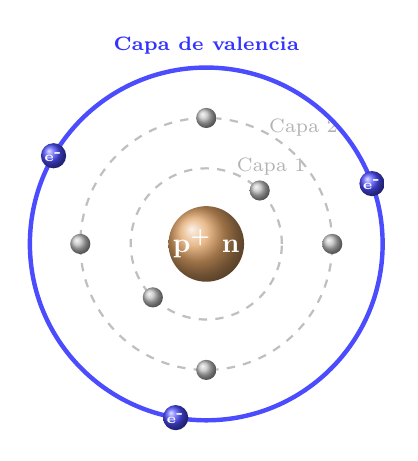
\begin{tikzpicture}[scale=0.40]
            % Nucleus with ochre gradient (only p+ and n)
            \shade[ball color=orange!80!black!60] (0,0) circle (1.2cm);
            \node[font=\normalsize\bfseries, white] at (0,0) {p\textsuperscript{+} n};
            % Shell 1 (radius 2.4)
            \draw[gray!50, thick, dashed] (0,0) circle (2.4cm);
            % Label Shell 1: between shell 1 (2.4) and shell 2 (4.0), at radius ~3.2
            \node[gray!60, font=\scriptsize] at (50:3.2) {Capa 1};
            % Shell 2 (radius 4.0, more separated)
            \draw[gray!50, thick, dashed] (0,0) circle (4.0cm);
            % Label Shell 2: between shell 2 (4.0) and valence (5.6), at radius ~4.8
            \node[gray!60, font=\scriptsize] at (50:4.8) {Capa 2};
            % Valence shell (radius 5.6, highlighted)
            \draw[blue!70, ultra thick] (0,0) circle (5.6cm);
            \node[blue!80, font=\scriptsize\bfseries] at (0, 6.3) {Capa de valencia};
            % Valence electrons (blue)
            \foreach \angle in {20, 150, 260} {
                \shade[ball color=blue!70] (\angle:5.6) circle (0.4cm);
                \node[white, font=\tiny\bfseries] at (\angle:5.6) {e\textsuperscript{-}};
            }
            % Inner electrons shell 1 (gray)
            \foreach \angle in {45, 225} {
                \shade[ball color=gray!50] (\angle:2.4) circle (0.32cm);
            }
            % Inner electrons shell 2 (gray)
            \foreach \angle in {0, 90, 180, 270} {
                \shade[ball color=gray!50] (\angle:4.0) circle (0.32cm);
            }
        \end{tikzpicture}
        \caption{Representación simplificada de un átomo.}
        \label{fig:atomo_valencia}
    \end{figure}
\end{minipage}
%
%    \begin{exercise} Answer the following questions:
%    \begin{enumerate}[label=\letraminuscula]
%        \item What are valence electrons?
%        \item Why do elements in the same group have similar chemical properties?
%        \item Sodium (\ch{Na}) and potassium (\ch{K}) are in the same group of the periodic table. Will they have similar chemical properties? Justify your answer.
%    \end{enumerate}
%    \begin{solu}
%        Answer the following questions:
%        \begin{enumerate}[label=\letraminuscula]
%        \item What are valence electrons?
%        \item Why do elements in the same group have similar chemical properties?
%        \item Sodium (\ch{Na}) and potassium (\ch{K}) are in the same group of the periodic table. Will they have similar chemical properties? Justify your answer.
%        \end{enumerate}
%        \negsubro{SOLUTION:}
%        \begin{enumerate}[label=\letraminuscula]
%            \item Valence electrons are the electrons found in the outermost shell of an atom. They are responsible for the chemical properties of the element.
%            \item Because they have the same electron configuration in their valence shell, that is, the same number of electrons in the outermost shell.
%            \item Yes, sodium and potassium will have similar chemical properties because they belong to the same group (group 1, alkali metals) and therefore have the same number of valence electrons (1 electron).
%        \end{enumerate}
%    \end{solu}
%\end{exercise}
\begin{definition}[Compuesto químico]
    Es una sustancia formada por dos o más elementos diferentes que están unidos químicamente en proporciones fijas.
\end{definition}
También es importante conocer la definición de molécula.
\begin{definition}[Molécula]
    es la unidad más pequeña de una sustancia química que conserva sus propiedades.
\end{definition}
Los diferentes tipos de estructuras que podemos encontrar son:
\begin{enumerate}[label=\numberballmDarkTeal]
        \item \negsubro{Átomos aislados}. \\
        Los átomos aislados se encuentran en los \textbf{gases nobles} debido a su alta estabilidad.
        Los gases nobles no tienden a combinarse con otros elementos porque su capa de valencia ya está completa.

        Los átomos aislados presentan las siguientes \textbf{propiedades físicas y químicas}:
        \begin{itemize}
            \item Son sustancias gaseosas a temperatura ambiente.
            \item No conducen la electricidad.
            \item No reaccionan con otras sustancias.
        \end{itemize}

        \item \negsubro{Moléculas diatómicas homonucleares}. \\
        Son moléculas formadas por dos átomos de un mismo elemento.
        Las moléculas diatómicas homonucleares que se encuentran en la naturaleza son:
        \ch{H2}, \ch{O2}, \ch{N2}, \ch{F2}, \ch{Cl2}, \ch{Br2}, y \ch{I2}.

        \item \negsubro{Moléculas heteronucleares}. \\
        Son moléculas que contienen dos o más elementos diferentes.

        Ejemplos: \ch{HCl}, \ch{H2S}, \ch{H2O}.

        \item \negsubro{Cristales}. \\
        Son sólidos cuyas partículas están dispuestas siguiendo un patrón que se repite en las tres dimensiones del espacio.
        \begin{itemize}
            \item \textbf{Cristales no metálicos}: como el grafito y el diamante, ambos formados por carbono pero con estructuras diferentes.
            \item \textbf{Cristales metálicos}: como el hierro, el cobre, etc.
        \end{itemize}

        % --- Comparative diagram: diamond vs graphite ---
        La Figura \eqref{fig:diamante_grafito} muestra cómo el carbono puede formar dos estructuras cristalinas muy diferentes.

        \begin{figure}[ht]
            \centering
            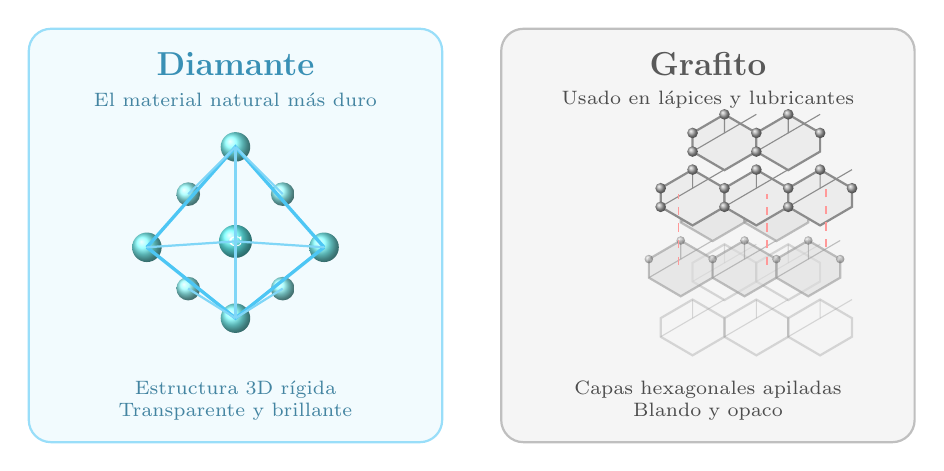
\begin{tikzpicture}[scale=0.75]
                % ===== DIAMOND =====
                % Decorative frame
                \fill[cyan!5, rounded corners=8pt] (-7.5,-1.8) rectangle (-0.5,5.2);
                \draw[cyan!40, thick, rounded corners=8pt] (-7.5,-1.8) rectangle (-0.5,5.2);
                \node[font=\large\bfseries, cyan!70!black] at (-4, 4.6) {Diamante};
                % Hardness icon
                \node[font=\scriptsize, cyan!60!black] at (-4, 4.0) {El material natural más duro};
                % 3D tetrahedral structure with perspective
                % Carbon atoms (shiny spheres)
                \shade[ball color=cyan!50] (-5.5,1.5) circle (0.25);
                \shade[ball color=cyan!50] (-2.5,1.5) circle (0.25);
                \shade[ball color=cyan!50] (-4,3.2) circle (0.25);
                \shade[ball color=cyan!50] (-4,0.3) circle (0.25);
                \shade[ball color=cyan!40] (-4.8,2.4) circle (0.2);

                \shade[ball color=cyan!40] (-3.2,2.4) circle (0.2);
                \shade[ball color=cyan!40] (-4.8,0.8) circle (0.2);
                \shade[ball color=cyan!40] (-3.2,0.8) circle (0.2);
                \shade[ball color=cyan!60] (-4,1.6) circle (0.28);
                \node[white, font=\tiny\bfseries] at (-4,1.6) {C};
                % Strong bonds (thick lines)
                \draw[cyan!70, very thick] (-5.5,1.5)--(-4,3.2)--(-2.5,1.5);
                \draw[cyan!70, very thick] (-5.5,1.5)--(-4,0.3)--(-2.5,1.5);
                \draw[cyan!70, very thick] (-4,3.2)--(-4,0.3);
                \draw[cyan!50, thick] (-4,1.6)--(-5.5,1.5);
                \draw[cyan!50, thick] (-4,1.6)--(-2.5,1.5);
                \draw[cyan!50, thick] (-4,1.6)--(-4,3.2);
                \draw[cyan!50, thick] (-4,1.6)--(-4,0.3);
                \draw[cyan!50, thick] (-4.8,2.4)--(-4,3.2);
                \draw[cyan!50, thick] (-3.2,2.4)--(-4,3.2);
                \draw[cyan!50, thick] (-4.8,0.8)--(-4,0.3);
                \draw[cyan!50, thick] (-3.2,0.8)--(-4,0.3);
                % Properties
                \node[font=\scriptsize, text width=3cm, align=center, cyan!60!black] at (-4,-1.1) {Estructura 3D rígida \\ Transparente y brillante};

                % ===== GRAPHITE =====
                \fill[gray!8, rounded corners=8pt] (0.5,-1.8) rectangle (7.5,5.2);
                \draw[gray!50, thick, rounded corners=8pt] (0.5,-1.8) rectangle (7.5,5.2);
                \node[font=\large\bfseries, gray!70!black] at (4, 4.6) {Grafito};
                \node[font=\scriptsize, gray!60!black] at (4, 4.0) {Usado en lápices y lubricantes};
                % Lower layer (lighter, depth effect)
                \begin{scope}[shift={(3.2,0.3)}, scale=0.9, opacity=0.35]
                    \foreach \hx/\hy in {0/0, 1.2/0, 2.4/0, 0.6/1.04, 1.8/1.04} {
                        \draw[gray!80, thick]
                        (\hx,\hy) -- ++(0.6,0.35) -- ++(0.6,-0.35)
                        -- ++(0,-0.35) -- ++(-0.6,-0.35) -- ++(-0.6,0.35) -- cycle;
                        \draw[gray!80] (\hx+0.6,\hy+0.35) -- ++(0,-0.35) -- ++(-0.6,-0.35);
                        \draw[gray!80] (\hx+0.6,\hy) -- ++(0.6,0.35);
                    }
                \end{scope}
                % Middle layer
                \begin{scope}[shift={(3.0,1.3)}, scale=0.9, opacity=0.6]
                    \foreach \hx/\hy in {0/0, 1.2/0, 2.4/0, 0.6/1.04, 1.8/1.04} {
                        \fill[gray!25]
                        (\hx,\hy) -- ++(0.6,0.35) -- ++(0.6,-0.35)
                        -- ++(0,-0.35) -- ++(-0.6,-0.35) -- ++(-0.6,0.35) -- cycle;
                        \draw[gray!80, thick]
                        (\hx,\hy) -- ++(0.6,0.35) -- ++(0.6,-0.35)
                        -- ++(0,-0.35) -- ++(-0.6,-0.35) -- ++(-0.6,0.35) -- cycle;
                        \draw[gray!80] (\hx+0.6,\hy+0.35) -- ++(0,-0.35) -- ++(-0.6,-0.35);
                        \draw[gray!80] (\hx+0.6,\hy) -- ++(0.6,0.35);
                    }
                    % Atoms at vertices of middle layer
                    \foreach \ax/\ay in {0/0, 0.6/0.35, 1.2/0, 1.8/0.35, 2.4/0, 3.0/0.35, 3.6/0,
                    0.6/1.04, 1.2/1.39, 1.8/1.04, 2.4/1.39, 3.0/1.04} {
                        \shade[ball color=gray!55] (\ax,\ay) circle (0.08);
                    }
                \end{scope}
                % Top layer (darker, foreground)
                \begin{scope}[shift={(3.2,2.5)}, scale=0.9]
                    \foreach \hx/\hy in {0/0, 1.2/0, 2.4/0, 0.6/1.04, 1.8/1.04} {
                        \fill[gray!15]
                        (\hx,\hy) -- ++(0.6,0.35) -- ++(0.6,-0.35)
                        -- ++(0,-0.35) -- ++(-0.6,-0.35) -- ++(-0.6,0.35) -- cycle;
                        \draw[gray!90, thick]
                        (\hx,\hy) -- ++(0.6,0.35) -- ++(0.6,-0.35)
                        -- ++(0,-0.35) -- ++(-0.6,-0.35) -- ++(-0.6,0.35) -- cycle;
                        \draw[gray!90] (\hx+0.6,\hy+0.35) -- ++(0,-0.35) -- ++(-0.6,-0.35);
                        \draw[gray!90] (\hx+0.6,\hy) -- ++(0.6,0.35);
                    }
                    % Atoms at vertices of top layer
                    \foreach \ax/\ay in {0/0, 0.6/0.35, 1.2/0, 1.8/0.35, 2.4/0, 3.0/0.35, 3.6/0,
                    0/-0.35, 1.2/-0.35, 2.4/-0.35,
                    0.6/1.04, 1.2/1.39, 1.8/1.04, 2.4/1.39, 3.0/1.04,
                    0.6/0.69, 1.8/0.69} {
                        \shade[ball color=gray!70] (\ax,\ay) circle (0.1);
                    }
                \end{scope}
                % Separation lines between layers (weak forces)
                \draw[red!40, dashed, thin] (3.5,1.2) -- (3.5,2.4);
                \draw[red!40, dashed, thin] (5.0,1.2) -- (5.0,2.4);
                \draw[red!40, dashed, thin] (6.0,1.5) -- (6.0,2.6);
                % Properties
                \node[font=\scriptsize, text width=4cm, align=center, gray!60!black] at (4,-1.1) {Capas hexagonales apiladas \\ Blando y opaco};
            \end{tikzpicture}
            \caption{El diamante y el grafito están hechos de carbono, pero sus diferentes estructuras les confieren propiedades muy distintas.}
            \label{fig:diamante_grafito}
        \end{figure}
\end{enumerate}


\section{Enlace químico}

Los átomos de diferentes elementos se unen para formar moléculas. Esta unión se llama \azul{\texttt{enlace químico}}. El enlace químico se produce porque la molécula formada es más estable que los átomos aislados.

En la naturaleza podemos encontrar principalmente 3 tipos de enlaces:

\begin{enumerate}[label=\numberballmDarkTeal]
\item \negsubro{Enlace iónico}: se produce por transferencia de electrones. Un elemento pierde electrones y otro los gana, formando un catión (ion positivo) y un anión (ion negativo). Ambos iones se mantienen unidos por la fuerza eléctrica de atracción.

Por ejemplo, el \ch{NaCl} se forma porque el \ch{Na} pierde un \el{} y se convierte en \ch{Na+}, mientras que el \ch{Cl} gana ese \el{} y se convierte en \ch{Cl-}, dando lugar a \ch{Na+ Cl-} (Figura \eqref{fig:enlace_ionico}).

% --- Ionic bond diagram ---
\begin{figure}[ht]
    \centering
    \begin{tikzpicture}[scale=0.85]
% Title
        \node[font=\bfseries\large, orange!70!black] at (1.5,3.9) {Formación del enlace iónico: \ch{NaCl}};

% === BEFORE ===
        \node[font=\small\bfseries, gray] at (-5.5,2.3) {ANTES};

% Na with electron shells
        \shade[ball color=blue!40] (-4.5,0) circle (0.6);
        \node[white, font=\bfseries] at (-4.5,0) {Na};
% Na valence shell (1 electron)
        \draw[blue!50, thick] (-4.5,0) circle (1.3);
        \shade[ball color=red!70] (-4.5,1.3) circle (0.15);
        \node[font=\tiny, blue!70] at (-4.5,-1.7) {11 e\textsuperscript{-} (2, 8, \textbf{1})};

% Cl with electron shells
        \shade[ball color=green!60!black!40] (-1.5,0) circle (0.7);
        \node[white, font=\bfseries] at (-1.5,0) {Cl};
% Cl valence shell (7 electrons)
        \draw[green!60!black, thick] (-1.5,0) circle (1.4);
        \foreach \a in {0,51.4,102.8,154.3,205.7,257.1,308.6} {
            \shade[ball color=red!70] ({-1.5+1.4*cos(\a)},{1.4*sin(\a)}) circle (0.15);
        }
        \node[font=\tiny, green!50!black] at (-1.5,-1.7) {17 e\textsuperscript{-} (2, 8, \textbf{7})};

% Transfer arrow (curved, with correct tip)
        \draw[-{Stealth[length=8pt, width=5pt]}, ultra thick, red!70, decorate, decoration={snake, amplitude=1.5pt, segment length=8pt, post length=8pt}]
        (-4.5,1.6) .. controls (-3,2.8) and (-2,2.8) .. (-1.5,1.7);
        \node[font=\small\bfseries, red!70] at (-3,3.0) {1 e\textsuperscript{-}};

% === Central arrow ===
        \draw[->, ultra thick, orange!70, >=stealth] (0.8,0) -- (2.2,0);
        \node[font=\tiny\bfseries, orange!70] at (1.5,0.4) {Forma};

% === AFTER ===
        \node[font=\small\bfseries, gray] at (5.5,2.3) {DESPUÉS};

% Na+ (smaller, lost electron)
        \shade[ball color=blue!60] (4,0) circle (0.5);
        \node[white, font=\bfseries] at (4,0) {Na\textsuperscript{+}};
% Decorative + sign
        \node[blue!70, font=\Large\bfseries] at (4,1.0) {$+$};

% Cl- (larger, gained electron)
        \shade[ball color=green!60!black!40] (7,0) circle (0.8);
        \node[white, font=\bfseries] at (7,0) {Cl\textsuperscript{-}};
% Decorative - sign
        \node[green!50!black, font=\Large\bfseries] at (7,1.2) {$-$};

% Attraction force (rays)
        \foreach \dy in {-0.3,0,0.3} {
            \draw[orange!80, thick, <->, >=stealth] (4.6,\dy) -- (6.1,\dy);
        }
        \node[font=\tiny\bfseries, orange!80] at (5.35,-0.8) {Atracción eléctrica};

% Final configuration
        \node[font=\tiny, blue!70] at (4,-1.7) {10 e\textsuperscript{-} (2, 8)};
        \node[font=\tiny, green!50!black] at (7,-1.7) {18 e\textsuperscript{-} (2, 8, 8)};

% Stability note
        \node[font=\tiny, gray, text width=3cm, align=center] at (5.5,-2.8) {Ambos tienen ahora \\ 8 e\textsuperscript{-} en su última capa};
    \end{tikzpicture}
    \caption{Formación del enlace iónico en el \ch{NaCl}. El sodio transfiere un electrón al cloro, formando iones que se atraen entre sí.}
    \label{fig:enlace_ionico}
\end{figure}

\item \negsubro{Enlace covalente}: es el enlace que se forma cuando dos átomos comparten electrones. El enlace formado se representa con una línea (\ch{-}), aunque a veces se omite por simplicidad.

Por ejemplo, el \ch{H} y el \ch{Cl} comparten electrones para formar un enlace covalente: \ch{H-Cl} (Figura \eqref{fig:enlace_covalente}).

% --- Covalent bond diagram ---
\begin{figure}[ht]
    \centering
    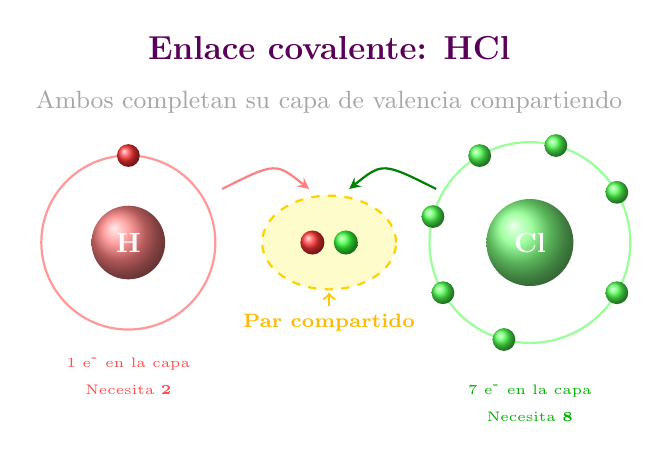
\begin{tikzpicture}[scale=0.85]
% Background
%\fill[violet!3, rounded corners=10pt] (-6,-3.5) rectangle (6,3.5);
% Title
        \node[font=\bfseries\large, violet!70!black] at (0,2.9) {Enlace covalente: \ch{HCl}};

% === H (left) ===
% H electron shell
        \draw[red!40, thick] (-3,0) circle (1.3);
        \shade[ball color=red!50] (-3,0) circle (0.55);
        \node[white, font=\bfseries] at (-3,0) {H};
% H's own electron
        \shade[ball color=red!80] (-3,1.3) circle (0.17);
        \node[font=\tiny, red!70] at (-3,-1.8) {1 e\textsuperscript{-} en la capa};
        \node[font=\tiny, red!70] at (-3,-2.2) {Necesita \textbf{2}};

% === Cl (right) ===
        \draw[green!40, thick] (3,0) circle (1.5);
        \shade[ball color=green!50] (3,0) circle (0.65);
        \node[white, font=\bfseries] at (3,0) {Cl};
% Cl's 7 valence electrons
        \foreach \a/\c in {30/green!70, 75/green!70, 120/green!70, 165/green!70, 210/green!70, 255/green!70, 330/green!70} {
            \shade[ball color=\c] ({3+1.5*cos(\a)},{1.5*sin(\a)}) circle (0.17);
        }
        \node[font=\tiny, green!70!black] at (3,-2.2) {7 e\textsuperscript{-} en la capa};
        \node[font=\tiny, green!70!black] at (3,-2.6) {Necesita \textbf{8}};

% === Sharing zone (center) ===
        \fill[yellow!40, opacity=0.5] (0,0) ellipse (1.0 and 0.7);
        \draw[yellow!70!orange, thick, dashed] (0,0) ellipse (1.0 and 0.7);
% Shared electron pair
        \shade[ball color=red!80] (-0.25,0) circle (0.18);
        \shade[ball color=green!80] (0.25,0) circle (0.18);
% Label
        \node[font=\scriptsize\bfseries, yellow!50!orange, fill=white, inner sep=2pt, rounded corners] at (0,-1.2) {Par compartido};
        \draw[->, yellow!60!orange, thick] (0,-0.95) -- (0,-0.75);

% Approach arrows
        \draw[->, thick, red!50, >=stealth] (-1.6,0.8) .. controls (-0.8,1.2) .. (-0.3,0.8);
        \draw[->, thick, green!50!black, >=stealth] (1.6,0.8) .. controls (0.8,1.2) .. (0.3,0.8);

% Result below
        \node[font=\small, gray!70, fill=white, inner sep=3pt, rounded corners=3pt] at (0,2.1)
            {Ambos completan su capa de valencia compartiendo};
    \end{tikzpicture}
    \caption{Enlace covalente en el \ch{HCl}. Ambos átomos comparten un par de electrones para completar su capa de valencia.}
    \label{fig:enlace_covalente}
\end{figure}

\item \negsubro{Enlace metálico}: es el enlace que se forma entre átomos de elementos metálicos. Los átomos de un metal comparten sus electrones de valencia, que se mueven libremente entre todos los átomos formando una ``nube de electrones''. Esto explica por qué los metales conducen la electricidad.

% --- Metallic bond diagram ---
La Figura \eqref{fig:enlace_metalico} ilustra este tipo de enlace.

\begin{figure}[ht]
    \centering
    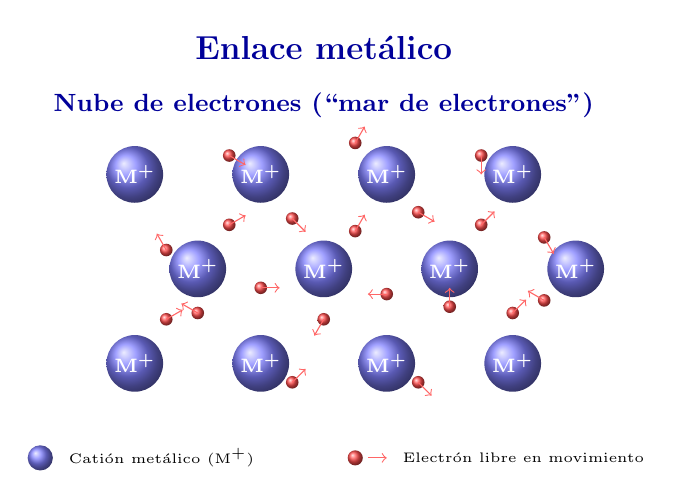
\begin{tikzpicture}[scale=0.8]
% General background
%\fill[blue!3, rounded corners=10pt] (-3.5,-3.5) rectangle (7.5,4.5);
% Title
        \node[font=\bfseries\large, blue!60!black] at (2,3.5) {Enlace metálico};

% Electron cloud (vibrant yellow background)
%\fill[yellow!25, rounded corners=12pt] (-2.5,-2.5) rectangle (6.5,3.0);
%\fill[yellow!15, rounded corners=12pt] (-2.8,-2.8) rectangle (6.8,3.2);
%\draw[yellow!60, thick, dashed, rounded corners=12pt] (-2.8,-2.8) rectangle (6.8,3.2);
        \node[font=\small\bfseries, blue!60!black, inner sep=3pt, rounded corners=3pt] at (2,2.6) {Nube de electrones (``mar de electrones'')};

% Lattice of metallic cations (ordered arrangement)
        \foreach \x/\y in {-1/-1.5, 1/-1.5, 3/-1.5, 5/-1.5, 0/0, 2/0, 4/0, 6/0, -1/1.5, 1/1.5, 3/1.5, 5/1.5} {
            \shade[ball color=blue!50] (\x,\y) circle (0.45);
            \node[white, font=\scriptsize\bfseries] at (\x,\y) {M\textsuperscript{+}};
        }

% Free electrons moving (with arrows to indicate movement)
        \foreach \x/\y/\ang in {
            0.5/0.7/30, 1.5/0.8/-45, 2.5/0.6/60, 3.5/0.9/-30,
            4.5/0.7/45, -0.5/0.3/120, 5.5/0.5/-60,
            0/-0.7/150, 2/-0.8/-120, 4/-0.6/90,
            1/-0.3/0, 3/-0.4/180, 5/-0.7/45,
            0.5/1.8/-30, 2.5/2.0/60, 4.5/1.8/-90,
            -0.5/-0.8/30, 5.5/-0.5/150, 1.5/-1.8/45, 3.5/-1.8/-45
        } {
            \shade[ball color=red!70] (\x,\y) circle (0.1);
            \draw[->, red!60, thin] (\x,\y) -- ++(\ang:0.3);
        }

% Legend
        \shade[ball color=blue!50] (-2.5,-3.0) circle (0.2);
        \node[font=\tiny, right] at (-2.2,-3.0) {Catión metálico (M\textsuperscript{+})};
        \shade[ball color=red!70] (2.5,-3.0) circle (0.12);
        \draw[->, red!60, thin] (2.7,-3.0) -- ++(0:0.3);
        \node[font=\tiny, right] at (3.1,-3.0) {Electrón libre en movimiento};
    \end{tikzpicture}
    \caption{En el enlace metálico, los cationes metálicos están rodeados por una nube de electrones en movimiento libre, lo que explica la conductividad eléctrica.}
    \label{fig:enlace_metalico}
\end{figure}

\end{enumerate}


\section{Masa atómica y masa molecular}

\subsection{Masa atómica}
Los átomos son partículas muy pequeñas, por lo que si midiéramos su masa en kilogramos, obtendríamos valores extremadamente pequeños. Por eso se creó una unidad especial que nos permite trabajar con estas masas de forma más sencilla.

Esta unidad se llama \azul{\texttt{unidad de masa atómica (uma)}} y se representa con \unit{\uma}.

\begin{definition}[Unidad de masa atómica]
    Es una doceava parte (\( \frac{1}{12} \)) de la masa de un átomo de \isotope{C}. Podemos decir que \( \qty{1}{\uma} \approx \qty{1.67e-27}{\kilogram} \).
\end{definition}

En muchos casos, la unidad de masa atómica se omite y solo se indica el número.

En la tabla periódica podemos encontrar las masas atómicas de cada elemento en uma.

Si quisiéramos saber la masa de un átomo en kilogramos, tendríamos que convertir uma a kilogramos utilizando la equivalencia dada anteriormente.

\subsection{Masa molecular}

Si lo que tenemos es una molécula, debemos calcular su masa molecular, es decir, la suma de las masas atómicas de todos los átomos que forman esa molécula. La masa molecular también se expresa en uma.

\begin{example}{}
    Vamos a calcular la masa molecular del \ch{H2O} sabiendo que las masas atómicas de los elementos son \( \ch{H} = 1 \) y \( \ch{O} = 16 \).
    \[
        \ch{H2O} \left\{\rule{0pt}{0.8cm}
                     \begin{array}{lcl}
                         \ch{H} &=& 2 \times \qty{1}{\uma} = \qty{2}{\uma} \\
                         \ch{O} &=& 1 \times \qty{16}{\uma} = \qty{16}{\uma} \\
                         \cline{1-3}
                         \multicolumn{3}{r}{\textbf{Total} = \qty{18}{\uma}}
                     \end{array}
        \right.
    \]
\end{example}

\begin{example}{}
    Vamos a calcular la masa molecular del \ch{H2SO4} sabiendo que las masas atómicas de los elementos son \( \ch{H} = 1 \), \( \ch{O} = 16 \), y \( \ch{S} = 32 \).
    \[
        \ch{H2SO4} \left\{\rule{0pt}{0.8cm}
                       \begin{array}{lcl}
                           \ch{H} &=& 2 \times \qty{1}{\uma} = \qty{2}{\uma} \\
                           \ch{S} &=& 1 \times \qty{32}{\uma} = \qty{32}{\uma} \\
                           \ch{O} &=& 4 \times \qty{16}{\uma} = \qty{64}{\uma} \\
                           \cline{1-3}
                           \multicolumn{3}{r}{\textbf{Total} = \qty{98}{\uma}}
                       \end{array}
        \right.
    \]
\end{example}



\begin{exercise}
    Indica cuál es la forma correcta de calcular la masa molecular del sulfato de calcio, \ch{CaSO4}:
    \begin{enumerate}[label=\letraminuscula]
\item Masa atómica del calcio + masa atómica del azufre + masa atómica del oxígeno.
\item Masa atómica del calcio + masa atómica del azufre + cuatro veces la masa atómica del oxígeno.
    \end{enumerate}
    \begin{solu}
        Indica cuál es la forma correcta de calcular la masa molecular del sulfato de calcio, \ch{CaSO4}:
        \begin{enumerate}[label=\letraminuscula]
\item Masa atómica del calcio + masa atómica del azufre + masa atómica del oxígeno.
\item Masa atómica del calcio + masa atómica del azufre + cuatro veces la masa atómica del oxígeno.
        \end{enumerate}
        Indica cuál es la forma correcta de calcular la masa molecular del sulfato de calcio, \ch{CaSO4}:

        La respuesta correcta es la \textbf{b)}: masa atómica del calcio + masa atómica del azufre + cuatro veces la masa atómica del oxígeno.

        En la fórmula \ch{CaSO4}, el subíndice 4 indica que hay 4 átomos de oxígeno, por lo que debemos multiplicar la masa atómica del oxígeno por 4.
    \end{solu}
\end{exercise}

\begin{exercise}
    El aire, compuesto principalmente por nitrógeno (\ch{N2}) y oxígeno (\ch{O2}), contiene cantidades variables de dióxido de carbono (\ch{CO2}). Busca las masas atómicas en la tabla periódica y calcula la masa molecular de estos tres gases.
    \begin{solu}
        El aire, compuesto principalmente por nitrógeno (\ch{N2}) y oxígeno (\ch{O2}), contiene cantidades variables de dióxido de carbono (\ch{CO2}). Busca las masas atómicas en la tabla periódica y calcula la masa molecular de estos tres gases.
        Calcula la masa molecular del \ch{N2}, \ch{O2}, y \ch{CO2}.

        Masas atómicas: \( \ch{N} = 14 \); \( \ch{O} = 16 \); \( \ch{C} = 12 \).

        \begin{itemize}
            \item \ch{N2}: \( 2 \times 14 = \qty{28}{\uma} \)
            \item \ch{O2}: \( 2 \times 16 = \qty{32}{\uma} \)
            \item \ch{CO2}: \( 1 \times 12 + 2 \times 16 = 12 + 32 = \qty{44}{\uma} \)
        \end{itemize}
    \end{solu}
\end{exercise}

\begin{exercise}
    Calcula la masa molecular del óxido de cinc (\ch{ZnO}), el nitrato de potasio (\ch{KNO3}), el sulfato de calcio (\ch{CaSO4}), el butano (\ch{C4H10}), y el carbonato de calcio (\ch{CaCO3}).
    \begin{solu}
        Calcula la masa molecular del óxido de cinc (\ch{ZnO}), el nitrato de potasio (\ch{KNO3}), el sulfato de calcio (\ch{CaSO4}), el butano (\ch{C4H10}), y el carbonato de calcio (\ch{CaCO3}).

        Calcula la masa molecular del \ch{ZnO}, \ch{KNO3}, \ch{CaSO4}, \ch{C4H10}, y \ch{CaCO3}.

        Masas atómicas: \( \ch{Zn} = 65 \); \( \ch{O} = 16 \); \( \ch{K} = 39 \); \( \ch{N} = 14 \); \( \ch{Ca} = 40 \); \( \ch{S} = 32 \); \( \ch{C} = 12 \); \( \ch{H} = 1 \).
        \begin{itemize}
            \item \ch{ZnO}: \( 65 + 16 = \qty{81}{\uma} \)
            \item \ch{KNO3}: \( 39 + 14 + 3 \times 16 = 39 + 14 + 48 = \qty{101}{\uma} \)
            \item \ch{CaSO4}: \( 40 + 32 + 4 \times 16 = 40 + 32 + 64 = \qty{136}{\uma} \)
            \item \ch{C4H10}: \( 4 \times 12 + 10 \times 1 = 48 + 10 = \qty{58}{\uma} \)
            \item \ch{CaCO3}: \( 40 + 12 + 3 \times 16 = 40 + 12 + 48 = \qty{100}{\uma} \)
        \end{itemize}
    \end{solu}
\end{exercise}

\begin{exercise}
    Busca las masas atómicas en la tabla periódica de esta unidad y ordena los siguientes compuestos de mayor a menor porcentaje de oxígeno: \ch{BaO}, \ch{K2O}, y \ch{CO2}.
    \begin{solu}
        Busca las masas atómicas en la tabla periódica de esta unidad y ordena los siguientes compuestos de mayor a menor porcentaje de oxígeno: \ch{BaO}, \ch{K2O}, y \ch{CO2}.

        Ordena \ch{BaO}, \ch{K2O}, y \ch{CO2} de mayor a menor porcentaje de oxígeno.

        Masas atómicas: \( \ch{Ba} = 137 \); \( \ch{K} = 39 \); \( \ch{C} = 12 \); \( \ch{O} = 16 \).

        \begin{itemize}
            \item \ch{BaO}: masa molecular \( = 137 + 16 = \qty{153}{\uma} \). Porcentaje de O \( = \frac{16}{153} \times 100 = 10.5 \% \)
            \item \ch{K2O}: masa molecular \( = 2 \times 39 + 16 = \qty{94}{\uma} \). Porcentaje de O \( = \frac{16}{94} \times 100 = 17{,}0\% \)
            \item \ch{CO2}: masa molecular \( = 12 + 2 \times 16 = \qty{44}{\uma} \). Porcentaje de O \( = \frac{32}{44} \times 100 = 72{,}7\% \)
        \end{itemize}

        Orden de mayor a menor porcentaje de oxígeno: \ch{CO2} > \ch{K2O} > \ch{BaO}.
    \end{solu}
\end{exercise}


\begin{exercise}
    Indica cuál de estas dos sustancias tiene mayor porcentaje de potasio: el cloruro de potasio (\ch{KCl}) o el nitrato de potasio (\ch{KNO3}).
    \begin{solu}
        Indica cuál de estas dos sustancias tiene mayor porcentaje de potasio: el cloruro de potasio (\ch{KCl}) o el nitrato de potasio (\ch{KNO3}).

        ¿Cuál tiene mayor porcentaje de potasio, el \ch{KCl} o el \ch{KNO3}?

        Masas atómicas: \( \ch{K} = 39 \); \( \ch{Cl} = 35{,}5 \); \( \ch{N} = 14 \); \( \ch{O} = 16 \).

        \begin{itemize}
            \item \ch{KCl}: masa molecular \( = 39 + \num{35.5} = \qty{74.5}{\uma} \). Porcentaje de K \( = \frac{39}{74.5} \times 100 = 52.3\% \)
            \item \ch{KNO3}: masa molecular \( = 39 + 14 + 3 \times 16 = \qty{101}{\uma} \). Porcentaje de K \( = \frac{39}{101} \times 100 = 38.6\% \)
        \end{itemize}

        El \ch{KCl} tiene mayor porcentaje de potasio (52.3\,\%) que el \ch{KNO3} (38.6\,\%).
    \end{solu}
\end{exercise}


\section{Cantidad de sustancia: el mol}

Dado que los átomos son muy pequeños y la materia está formada por cantidades enormes de ellos, se creó una unidad para agrupar muchos átomos y así poder trabajar con cantidades más fáciles de manejar.

Con este propósito se creó la unidad de sustancia llamada \azul{\texttt{mol}} y se representa con \( \bm{n} \).

\begin{definition}[Mol]
    Es la cantidad de sustancia que contiene \num{6.022e23} entidades elementales, que pueden ser átomos, moléculas, iones, electrones, u otras partículas.
\end{definition}

Podemos entender el mol como una ``caja'' que siempre contiene \num{6.022e23} ``cosas''.

Este número tan grande se llama \azul{\texttt{constante de Avogadro}} y se representa con \( \bm{N_A} \).

\begin{equation*}
    N_A = \num{6.022e23}\ \dfrac{\text{partículas}}{\unit{\mol}}
\end{equation*}

% --- Visual diagram of the mole ---
La Figura \eqref{fig:mol_particulas} ilustra este concepto.

\begin{figure}[ht]
    \centering
    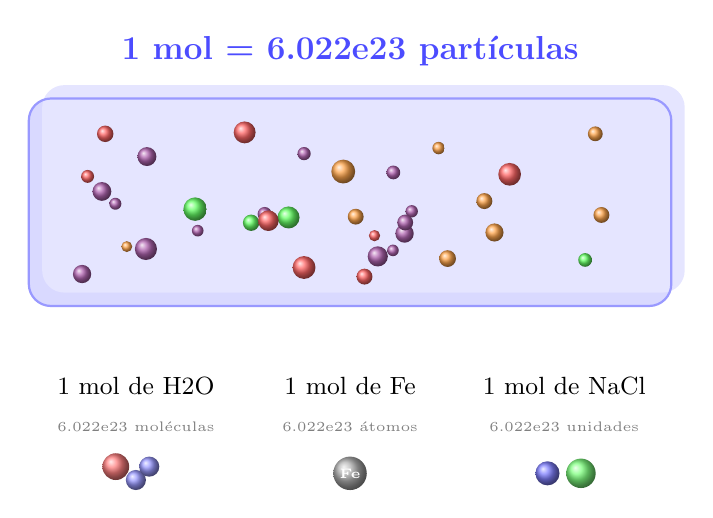
\begin{tikzpicture}[scale=0.85]
% General background
%\fill[blue!3, rounded corners=12pt] (-5.5,-3.5) rectangle (5.5,4.5);

% Large title
        \node[font=\large\bfseries, blue!70] at (0,3.5) {1 mol = \num{6.022e23} partículas};

% Main box with 3D effect
        \fill[blue!15, rounded corners=8pt] (-4.8,-0.3) rectangle (4.8,2.8);
        \fill[blue!10, rounded corners=8pt] (-4.6,-0.1) rectangle (5.0,3.0);
        \draw[blue!40, thick, rounded corners=8pt] (-4.8,-0.3) rectangle (4.8,2.8);

% Particles of various colors and sizes to make it visual
        \pgfmathsetseed{42}
        \foreach \i in {1,...,35} {
            \pgfmathsetmacro{\rx}{-4.2 + rnd*8.0}
            \pgfmathsetmacro{\ry}{0.1 + rnd*2.2}
            \pgfmathsetmacro{\rr}{0.08 + rnd*0.1}
            \pgfmathsetmacro{\rc}{int(rnd*4)}
            \ifnum
                \rc=0
                \shade[ball color=orange!70] (\rx,\ry) circle (\rr);
            \fi
            \ifnum
                \rc=1
                \shade[ball color=red!60] (\rx,\ry) circle (\rr);
            \fi
            \ifnum
                \rc=2
                \shade[ball color=green!60] (\rx,\ry) circle (\rr);
            \fi
            \ifnum
                \rc=3
                \shade[ball color=violet!60] (\rx,\ry) circle (\rr);
            \fi
        }

% Central Avogadro's number (with white background for readability)
%\node[font=\Large\bfseries, fill=white, fill opacity=0.85, text opacity=1, inner sep=6pt, rounded corners=4pt] at (8,1.3) {\( \num{6.022e23} \) particles};

% Arrow pointing to equals
%\node[font=\LARGE\bfseries, blue!60] at (0,3.1) {$=$};

% Three examples below
% Example 1: water
        \node[font=\small, align=center] at (-3.2,-1.5) {1 mol de \ch{H2O}};
        \node[font=\tiny, align=center, gray] at (-3.2,-2.1) {\num{6.022e23} moléculas};
        \shade[ball color=red!50] (-3.5,-2.7) circle (0.2);
        \shade[ball color=blue!40] (-3.2,-2.9) circle (0.15);
        \shade[ball color=blue!40] (-3.0,-2.7) circle (0.15);

% Example 2: iron
        \node[font=\small, align=center] at (0,-1.5) {1 mol de \ch{Fe}};
        \node[font=\tiny, align=center, gray] at (0,-2.1) {\num{6.022e23} átomos};
        \shade[ball color=gray!60] (0,-2.8) circle (0.25);
        \node[white, font=\tiny\bfseries] at (0,-2.8) {Fe};

% Example 3: NaCl
        \node[font=\small, align=center] at (3.2,-1.5) {1 mol de \ch{NaCl}};
        \node[font=\tiny, align=center, gray] at (3.2,-2.1) {\num{6.022e23} unidades};
        \shade[ball color=blue!50] (2.95,-2.8) circle (0.18);
        \shade[ball color=green!50] (3.45,-2.8) circle (0.22);
    \end{tikzpicture}
    \caption{Un mol siempre contiene \num{6.022e23} partículas, independientemente de la sustancia.}
    \label{fig:mol_particulas}
\end{figure}

\begin{example}{}
    Calcula cuántos moles hay en \num{6.022e21} átomos de \ch{Ag}. Haremos el cálculo utilizando factores de conversión.
    \begin{equation*}
        \num{6.022e21}\ \cancelred{\text{átomos de \ch{Ag}}} \cdot \dfrac{\qty{1}{\mole}\ \text{de \ch{Ag}}}{\num{6.022e23}\ \cancelred{\text{átomos de \ch{Ag}}}} = \qty{0.01}{\mol}\ \text{de \ch{Ag}}
    \end{equation*}
\end{example}

\begin{example}{}
    ¿Cuántas moléculas hay en \qty{0.5}{\mole} de moléculas de \ch{H2O}?

    Ahora tenemos un compuesto (formado por \ch{H} y \ch{O}) y no un elemento, por lo que hablaremos de moléculas y no de átomos.
    \begin{equation*}
        0.5\ \cancelred{\unit{\mole}\ \text{de \ch{H2O}}} \cdot \dfrac{\qty{6.022e23}{\text{moléculas}}\ \text{de \ch{H2O}}}{1\ \cancelred{\unit{\mole} \ \text{de \ch{H2O}}}} = \qty{3.011e23}{\text{moléculas}}\ \text{de \ch{H2O}}
    \end{equation*}
\end{example}



\begin{exercise}
    ¿Cuántas moléculas hay en \qty{0.5}{\mole} de moléculas de oxígeno (\ch{O2})? ¿Qué cantidad de sustancia, en moles, hay en \num{6.022e23} átomos de oxígeno?
    \begin{solu}
        ¿Cuántas moléculas hay en \qty{0.5}{\mole} de moléculas de oxígeno (\ch{O2})? ¿Qué cantidad de sustancia, en moles, hay en \num{6.022e23} átomos de oxígeno?

        ¿Cuántas moléculas hay en \qty{0.5}{\mole} de \ch{O2}? ¿Qué cantidad de sustancia hay en \num{6.022e23} átomos de oxígeno?

        \textbf{Parte 1:}
        \begin{equation*}
            0{,}5\ \cancelred{\unit{\mole}\ \text{de \ch{O2}}} \cdot \dfrac{\qty{6.022e23}{\text{moléculas de \ch{O2}}}}{1\ \cancelred{\unit{\mole}\ \text{de \ch{O2}}}} = \qty{3.011e23}{\text{moléculas de \ch{O2}}}
        \end{equation*}

        \textbf{Parte 2:}
        \begin{equation*}
            \num{6.022e23}\ \cancelred{\text{átomos de O}} \cdot \dfrac{1\ \unit{\mole}\ \text{de O}}{\num{6.022e23}\ \cancelred{\text{átomos de O}}} = \qty{1}{\mole}\ \text{de átomos de oxígeno}
        \end{equation*}
    \end{solu}
\end{exercise}

\begin{exercise}
    ¿Dónde hay más moléculas, en 1 mol de hidrógeno (\ch{H2}) o en 1 mol de agua (\ch{H2O})?
    \begin{solu}
        ¿Dónde hay más moléculas, en 1 mol de \ch{H2} o en 1 mol de \ch{H2O}?

        En ambos casos hay el mismo número de moléculas: \num{6.022e23} moléculas. Un mol siempre contiene el mismo número de entidades (número de Avogadro), independientemente de la sustancia.
    \end{solu}
\end{exercise}

\begin{exercise}
    Indica si la siguiente afirmación es verdadera o falsa y justifica tu respuesta:
    ``En 1 mol de átomos de helio hay el mismo número de átomos de helio que moléculas hay en 1 mol de butano, \ch{C4H10}.''
    \begin{solu}
        Indica si la siguiente afirmación es verdadera o falsa y justifica tu respuesta:
        ``En 1 mol de átomos de helio hay el mismo número de átomos de helio que moléculas hay en 1 mol de butano, \ch{C4H10}.''

        Verdadero o falso: ``En 1 mol de átomos de helio hay el mismo número de átomos que moléculas hay en 1 mol de butano.''

        \textbf{Verdadero.} Un mol siempre contiene \num{6.022e23} entidades elementales, ya sean átomos, moléculas, u otras partículas. Por lo tanto, 1 mol de átomos de helio contiene \num{6.022e23} átomos de helio y 1 mol de butano contiene \num{6.022e23} moléculas de butano. Ambas cantidades son iguales.
    \end{solu}
\end{exercise}

\begin{exercise}
    ¿Cuántos átomos de hidrógeno hay en \qty{2}{\mole} de agua (\ch{H2O})?
    \begin{solu}
        ¿Cuántos átomos de hidrógeno hay en \qty{2}{\mole} de \ch{H2O}?

        Primero calculamos el número de moléculas de agua:
        \begin{equation*}
            2\ \cancelred{\unit{\mole}\ \text{de \ch{H2O}}} \cdot \dfrac{\num{6.022e23}\ \text{moléculas de \ch{H2O}}}{1\ \cancelred{\unit{\mole}\ \text{de \ch{H2O}}}} = \num{12.044e23}\ \text{moléculas de \ch{H2O}}
        \end{equation*}

        Cada molécula de \ch{H2O} tiene 2 átomos de hidrógeno, por lo tanto:
        \begin{equation*}
            \num{12.044e23}\ \cancelred{\text{moléculas de \ch{H2O}}} \cdot \dfrac{2\ \text{átomos de H}}{1\ \cancelred{\text{molécula de \ch{H2O}}}} = \num{24.088e23}\ \text{átomos de H} = \num{2.4088e24}\ \text{átomos de H}
        \end{equation*}
    \end{solu}
\end{exercise}


\section{Masa molar}

Como su nombre indica, la masa molar es la masa de 1 mol de una sustancia (átomos, moléculas, iones...) y se expresa en \unit{\g\per\mole}. La masa molar suele representarse con \( M_w \).

En términos prácticos, podemos decir que \qty{1}{\uma} = \qty{1}{\g\per\mole}. Por lo tanto, si sabemos que el \ch{Na} tiene una masa atómica de \qty{23}{\uma}, podemos decir que 1 mol de sodio tiene una masa de \qty{23}{\g}, es decir, la masa molar del sodio es \qty{23}{\g\per\mole}.

Esta equivalencia es muy útil si queremos calcular los moles de una sustancia a partir de su masa, utilizando factores de conversión o la fórmula:
\begin{equation*}
    n\ (\text{número de moles}) = \dfrac{\text{masa en gramos}}{\text{masa molar}}
\end{equation*}

Si usamos abreviaturas:
\begin{equation*}
    n = \dfrac{m\ (\text{g})}{M_w}
\end{equation*}

La Figura \eqref{fig:masa_mol_particulas} resume las conversiones entre masa, moles, y partículas.

% --- Summary diagram of the mass-mole-particles relationship ---
\begin{figure}[ht]
    \centering
    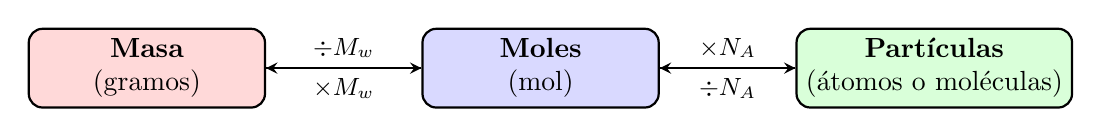
\begin{tikzpicture}[
        box/.style={rectangle, draw, thick, fill=#1, rounded corners=5pt, minimum width=3cm, minimum height=1cm, align=center},
        arr/.style={->, thick, >=stealth}
    ]
        \node[box=red!15] (masa) at (-5,0) {\textbf{Masa} \\ (gramos)};
        \node[box=blue!15] (mol) at (0,0) {\textbf{Moles} \\ (mol)};
        \node[box=green!15] (part) at (5,0) {\textbf{Partículas} \\ (átomos o moléculas)};

        \draw[arr] (masa) -- node[above, font=\small] {\( \div M_w \)} (mol);
        \draw[arr] (mol) -- node[below, font=\small] {\( \times M_w \)} (masa);
        \draw[arr] (mol) -- node[above, font=\small] {\( \times N_A \)} (part);
        \draw[arr] (part) -- node[below, font=\small] {\( \div N_A \)} (mol);
    \end{tikzpicture}
    \caption{Relación entre masa, moles, y número de partículas.}
    \label{fig:masa_mol_particulas}
\end{figure}

\begin{example}{}

    Calcula los moles de \ch{CH4} contenidos en \qty{48}{\g}.

    \datos{}: Las masas atómicas son: \( \ch{H} = 1 \); \( \ch{C} = 12 \).

    Primero debemos calcular la masa molar. Como hemos dicho, la masa molar tiene el mismo valor numérico que la masa molecular, pero en \unit{\g\per\mole} en lugar de uma.

    \[
        \ch{CH4} \left\{\rule{0pt}{0.8cm}
                     \begin{array}{lcl}
                         \ch{H} &=& 4 \times \qty{1}{\uma} = \qty{4}{\uma} \\
                         \ch{C} &=& 1 \times \qty{12}{\uma} = \qty{12}{\uma} \\
                         \cline{1-3}
                         \multicolumn{3}{r}{\textbf{Total} = \qty{16}{\uma} }
                     \end{array}
        \right.
    \]

    Por lo tanto, la masa molar del \ch{CH4} es \qty{16}{\g\per\mole}.

    Aplicando la fórmula:
    \begin{equation*}
        n = \dfrac{m}{M_w} = \dfrac{48}{16} = \qty{3}{\mole} \text{ de \ch{CH4}}
    \end{equation*}
\end{example}



\begin{exercise}
    Un matraz contiene \qty{100}{\g} de carbonato de calcio, \ch{CaCO3}. Calcula la cantidad de esta sustancia, en moles, en dicho recipiente.
    \begin{solu}
        Un matraz contiene \qty{100}{\g} de carbonato de calcio, \ch{CaCO3}. Calcula la cantidad de esta sustancia, en moles, en dicho recipiente.

        Calcula los moles en \qty{100}{\g} de \ch{CaCO3}.

        Masas atómicas: \( \ch{Ca} = 40 \); \( \ch{C} = 12 \); \( \ch{O} = 16 \).

        Masa molar del \ch{CaCO3}: \( 40 + 12 + 3 \times 16 = \qty{100}{\g\per\mole} \).

        \begin{equation*}
            n = \dfrac{m}{M_w} = \dfrac{100}{100} = \qty{1}{\mole} \text{ de \ch{CaCO3}}
        \end{equation*}
    \end{solu}
\end{exercise}

\begin{exercise}
    ¿Qué cantidad en moles de nitrógeno gaseoso, \ch{N2}, hay en \qty{56}{\g} de esta sustancia? ¿Cuántas moléculas hay? ¿Y cuántos átomos?
    \begin{solu}
        ¿Qué cantidad en moles de nitrógeno gaseoso, \ch{N2}, hay en \qty{56}{\g} de esta sustancia? ¿Cuántas moléculas hay? ¿Y cuántos átomos?

        Calcula los moles, las moléculas, y los átomos en \qty{56}{\g} de \ch{N2}.

        Masa atómica: \( \ch{N} = 14 \). Masa molar del \ch{N2}: \( 2 \times 14 = \qty{28}{\g\per\mole} \).

        \textbf{Moles:}
        \begin{equation*}
            n = \dfrac{56}{28} = \qty{2}{\mole} \text{ de \ch{N2}}
        \end{equation*}

        \textbf{Moléculas:}
        \begin{equation*}
            2\ \cancelred{\unit{\mole}} \times \num{6.022e23}\ \dfrac{\text{moléculas}}{\cancelred{\unit{\mole}}} = \num{12.044e23} = \num{1.2044e24} \text{ moléculas de \ch{N2}}
        \end{equation*}

        \textbf{Átomos:} Cada molécula de \ch{N2} tiene 2 átomos de N:
        \begin{equation*}
            \num{1.2044e24} \times 2 = \num{2.4088e24} \text{ átomos de N}
        \end{equation*}
    \end{solu}
\end{exercise}

\begin{exercise}
    Calcula las masas molares de las siguientes sustancias: bromo (\ch{Br2}), yoduro de potasio (\ch{KI}), carbonato de calcio (\ch{CaCO3}), y carbonato de sodio (\ch{Na2CO3}).
    \begin{solu}
        Calcula las masas molares de las siguientes sustancias: bromo (\ch{Br2}), yoduro de potasio (\ch{KI}), carbonato de calcio (\ch{CaCO3}), y carbonato de sodio (\ch{Na2CO3}).

        Calcula las masas molares del \ch{Br2}, \ch{KI}, \ch{CaCO3}, y \ch{Na2CO3}.

        Masas atómicas: \( \ch{Br} = 80 \); \( \ch{K} = 39 \); \( \ch{I} = 127 \); \( \ch{Ca} = 40 \); \( \ch{C} = 12 \); \( \ch{O} = 16 \); \( \ch{Na} = 23 \).
        \begin{itemize}
            \item \ch{Br2}: \( 2 \times 80 = \qty{160}{\g\per\mole} \)
            \item \ch{KI}: \( 39 + 127 = \qty{166}{\g\per\mole} \)
            \item \ch{CaCO3}: \( 40 + 12 + 3 \times 16 = \qty{100}{\g\per\mole} \)
            \item \ch{Na2CO3}: \( 2 \times 23 + 12 + 3 \times 16 = 46 + 12 + 48 = \qty{106}{\g\per\mole} \)
        \end{itemize}
    \end{solu}
\end{exercise}

\begin{exercise}
    ¿Qué cantidad de sustancia, en moles, hay en \qty{66}{\g} de dióxido de carbono, \ch{CO2}?
    \begin{solu}
        ¿Qué cantidad de sustancia, en moles, hay en \qty{66}{\g} de dióxido de carbono, \ch{CO2}?

        Calcula los moles en \qty{66}{\g} de \ch{CO2}.

        Masas atómicas: \( \ch{C} = 12 \); \( \ch{O} = 16 \).

        Masa molar del \ch{CO2}: \( 12 + 2 \times 16 = \qty{44}{\g\per\mole} \).

        \begin{equation*}
            n = \dfrac{66}{44} = \qty{1.5}{\mole} \text{ de \ch{CO2}}
        \end{equation*}
    \end{solu}
\end{exercise}

\begin{exercise}
    Calcula la masa de:
    \begin{enumerate}[label=\letraminuscula]
\item \qty{2}{\mole} de cloruro de hidrógeno, \ch{HCl}.
\item \qty{2}{\mole} de agua, \ch{H2O}.
\item \qty{1.5}{\mole} de ácido sulfúrico, \ch{H2SO4}.
\item \qty{0.5}{\mole} de cloro, \ch{Cl2}.
    \end{enumerate}
    \begin{solu}
        Calcula la masa de:
        \begin{enumerate}[label=\letraminuscula]
\item \qty{2}{\mole} de cloruro de hidrógeno, \ch{HCl}.
\item \qty{2}{\mole} de agua, \ch{H2O}.
\item \qty{1.5}{\mole} de ácido sulfúrico, \ch{H2SO4}.
\item \qty{0.5}{\mole} de cloro, \ch{Cl2}.
        \end{enumerate}

        Calcula la masa de cada sustancia. Usamos \( m = n \times M_w \).

        Masas atómicas: \( \ch{H} = 1 \); \( \ch{Cl} = 35{,}5 \); \( \ch{O} = 16 \); \( \ch{S} = 32 \).

        \begin{enumerate}[label=\letraminuscula]
\item \ch{HCl}: \( M_w = 1 + 35{,}5 = \qty{36.5}{\g\per\mole} \). \( m = 2 \times 36{,}5 = \qty{73}{\g} \).
\item \ch{H2O}: \( M_w = 2 \times 1 + 16 = \qty{18}{\g\per\mole} \). \( m = 2 \times 18 = \qty{36}{\g} \).
\item \ch{H2SO4}: \( M_w = 2 + 32 + 64 = \qty{98}{\g\per\mole} \). \( m = 1{,}5 \times 98 = \qty{147}{\g} \).
\item \ch{Cl2}: \( M_w = 2 \times 35{,}5 = \qty{71}{\g\per\mole} \). \( m = 0{,}5 \times 71 = \qty{35.5}{\g} \).
        \end{enumerate}
    \end{solu}
\end{exercise}

\begin{exercise}
    ¿Qué cantidad en moles de sustancia hay en \qty{36.5}{\g} de \ch{HCl}, en \qty{73}{\g} de \ch{HCl}, y en \qty{146}{\g} de \ch{HCl}?
    \begin{solu}
        ¿Qué cantidad en moles de sustancia hay en \qty{36.5}{\g} de \ch{HCl}, en \qty{73}{\g} de \ch{HCl}, y en \qty{146}{\g} de \ch{HCl}?

        Calcula los moles en \qty{36.5}{\g}, \qty{73}{\g}, y \qty{146}{\g} de \ch{HCl}.

        Masa molar del \ch{HCl}: \( 1 + 35{,}5 = \qty{36.5}{\g\per\mole} \).

        \begin{itemize}
            \item \( n = \dfrac{36{,}5}{36{,}5} = \qty{1}{\mole} \)
            \item \( n = \dfrac{73}{36{,}5} = \qty{2}{\mole} \)
            \item \( n = \dfrac{146}{36{,}5} = \qty{4}{\mole} \)
        \end{itemize}
    \end{solu}
\end{exercise}


\section{Ley de los gases ideales}

Las tres leyes de los gases (la Ley de Gay-Lussac, la Ley de Charles, y la Ley de Boyle-Mariotte) se pueden combinar en una sola ley llamada la \textbf{Ley de los gases ideales}. Esta ley relaciona la presión, el volumen, y la temperatura con la cantidad de sustancia en moles.

La expresión matemática de esta ley es:
\vspace{20pt}
\begin{centeredequation}
    \eqnmarkbox[blue]{presion}{p}
    \cdot
    \eqnmarkbox[red]{volumen}{V}
    =
    \eqnmarkbox[mDarkTeal]{moles}{n}
    \cdot
    \eqnmarkbox[orange]{constante}{R}
    \cdot
    \eqnmarkbox[violet]{temperatura}{T}
\end{centeredequation}
\vspace{25pt}
\annotate[yshift=1em]{left}{presion}{Presión en \unit{\atmosphere}}
\annotate[yshift=-0.5em]{below,left}{volumen}{Volumen en \unit{\litre}}
\annotate[yshift=1em]{}{moles}{número de moles}
\annotate[yshift=-2em]{below,left}{constante}{Constante de los gases ideales; R = \ctegases{}}
\annotate[yshift=-1em]{below}{temperatura}{Temperatura en \unit{\kelvin}}
\begin{exercise}
    Tenemos \qty{3}{\mole} de un gas ideal a una temperatura de \qty{300}{\kelvin} y una presión de \qty{2}{\atmosphere}. Calcula el volumen que ocupa el gas.
    \begin{solu}
        Tenemos \qty{3}{\mole} de un gas ideal a una temperatura de \qty{300}{\kelvin} y una presión de \qty{2}{\atmosphere}. Calcula el volumen que ocupa el gas.

        Calcula el volumen de \qty{3}{\mole} de gas a \qty{300}{\kelvin} y \qty{2}{\atmosphere}.

        Despejamos \( V \) de la ley de los gases ideales:
        \begin{equation*}
            V = \dfrac{nRT}{p} = \dfrac{3 \times 0{,}082 \times 300}{2} = \dfrac{73{,}8}{2} = \qty{36.9}{\litre}
        \end{equation*}
    \end{solu}
\end{exercise}
\begin{exercise}
    Un gas ideal ocupa un volumen de \qty{10}{\litre} a una presión de \qty{1.5}{\atmosphere} y una temperatura de \qty{350}{\kelvin}. ¿Cuántos moles de gas hay?
    \begin{solu}
        Un gas ideal ocupa un volumen de \qty{10}{\litre} a una presión de \qty{1.5}{\atmosphere} y una temperatura de \qty{350}{\kelvin}. ¿Cuántos moles de gas hay?

        Calcula los moles de un gas que ocupa \qty{10}{\litre} a \qty{1.5}{\atmosphere} y \qty{350}{\kelvin}.

        Despejamos \( n \):
        \begin{equation*}
            n = \dfrac{pV}{RT} = \dfrac{1{,}5 \times 10}{0{,}082 \times 350} = \dfrac{15}{28{,}7} = \qty{0.52}{\mole}
        \end{equation*}
    \end{solu}
\end{exercise}
\begin{exercise}
    ¿Qué volumen en mL ocupa un gas ideal si \qty{0.553}{\mol} están a una temperatura de \qty{1226.49}{\kelvin} y una presión de \qty{4935}{\mmHg}?
    \begin{solu}
        ¿Qué volumen en mL ocupa un gas ideal si \qty{0.553}{\mol} están a una temperatura de \qty{1226.49}{\kelvin} y una presión de \qty{4935}{\mmHg}?

        Aplicamos la ley de los gases ideales $PV = nRT$, despejando el volumen:
        \begin{equation*}
            V = \frac{nRT}{P}
        \end{equation*}
        \textbf{Paso 1: Identificar los datos.}
        \begin{align*}
            n &= \qty{0.553}{\mol} \\
            T &= \qty{1226.49}{\kelvin} \\
            P &= \qty{4935}{\mmHg} \\
            R &= \qty{0.082057}{\atm\liter\per\mol\per\kelvin}
        \end{align*}
        \textbf{Paso 2: Convertir la presión a atm.}

        La constante $R$ está expresada en unidades de atm, así que debemos convertir la presión de mmHg a atm usando el factor de conversión $\qty{1}{\atm} = \qty{760}{\mmHg}$:
        \begin{equation*}
            P = \qty{4935}{\mmHg} \times \frac{\qty{1}{\atm}}{\qty{760}{\mmHg}} = \qty{6.4934}{\atm}
        \end{equation*}
        \textbf{Paso 3: Sustituir en la ecuación y calcular $V$ en litros.}
        \begin{equation*}
            V = \frac{nRT}{P} = \frac{\qty{0.553}{\mol} \times \qty{0.082057}{\atm\liter\per\mol\per\kelvin} \times \qty{1226.49}{\kelvin}}{\qty{6.4934}{\atm}} = \qty{8.573}{\liter}
        \end{equation*}
        \textbf{Paso 4: Convertir el volumen a mL.}

        Como el problema pide el volumen en mL, usamos el factor de conversión $\qty{1}{\liter} = \qty{1000}{\mL}$:
        \begin{equation*}
            V = \qty{8.573}{\liter} \times \frac{\qty{1000}{\mL}}{\qty{1}{\liter}} = \boxed{\qty{8573}{\mL}}
        \end{equation*}
    \end{solu}
\end{exercise}
\begin{exercise}
    ¿Cuál es la temperatura en \unit{\kelvin} de un gas ideal, si \qty{0.405}{\mole} ocupan un volumen de \qty{7720}{\mL} a una presión de \qty{790}{\mmHg}?
    \begin{solu}
        ¿Cuál es la temperatura en \unit{\kelvin} de un gas ideal, si \qty{0.405}{\mole} ocupan un volumen de \qty{7720}{\mL} a una presión de \qty{790}{\mmHg}?

        Aplicamos la ley de los gases ideales $PV = nRT$, despejando la temperatura:
        \begin{equation*}
            T = \frac{PV}{nR}
        \end{equation*}
        \textbf{Paso 1: Identificar los datos.}
        \begin{align*}
            n &= \qty{0.405}{\mol} \\
            V &= \qty{7720}{\mL} \\
            P &= \qty{790}{\mmHg} \\
            R &= \qty{0.082057}{\atm\liter\per\mol\per\kelvin}
        \end{align*}
        \textbf{Paso 2: Convertir la presión a atm.}

        Convertimos mmHg a atm usando el factor de conversión $\qty{1}{\atm} = \qty{760}{\mmHg}$:
        \begin{equation*}
            P = \qty{790}{\mmHg} \times \frac{\qty{1}{\atm}}{\qty{760}{\mmHg}} = \qty{1.03947}{\atm}
        \end{equation*}
        \textbf{Paso 3: Convertir el volumen a litros.}

        La constante $R$ tiene litros en sus unidades, así que convertimos mL a L usando el factor de conversión $\qty{1}{\liter} = \qty{1000}{\mL}$:
        \begin{equation*}
            V = \qty{7720}{\mL} \times \frac{\qty{1}{\liter}}{\qty{1000}{\mL}} = \qty{7.720}{\liter}
        \end{equation*}
        \textbf{Paso 4: Sustituir en la ecuación y calcular $T$.}
        \begin{equation*}
            T = \frac{PV}{nR} = \frac{\qty{1.03947}{\atm} \times \qty{7.720}{\liter}}{\qty{0.405}{\mol} \times \qty{0.082057}{\atm\liter\per\mol\per\kelvin}} = \boxed{\qty{241.5}{\kelvin}}
        \end{equation*}
    \end{solu}
\end{exercise}
\begin{exercise}
    ¿Cuál es la temperatura en \unit{\degreeCelsius} de un gas ideal, si \qty{0.746}{\mol} ocupan un volumen de \qty{9890}{\mL} a una presión de \qty{1.41}{\atmosphere}?
    \begin{solu}
        ¿Cuál es la temperatura en \unit{\degreeCelsius} de un gas ideal, si \qty{0.746}{\mol} ocupan un volumen de \qty{9890}{\mL} a una presión de \qty{1.41}{\atmosphere}?

        Aplicamos la ley de los gases ideales $PV = nRT$, despejando la temperatura:
        \begin{equation*}
            T = \frac{PV}{nR}
        \end{equation*}
        \textbf{Paso 1: Identificar los datos.}
        \begin{align*}
            n &= \qty{0.746}{\mol} \\
            V &= \qty{9890}{\mL} \\
            P &= \qty{1.41}{\atm} \\
            R &= \qty{0.082057}{\atm\liter\per\mol\per\kelvin}
        \end{align*}
        \textbf{Paso 2: Convertir el volumen a litros.}

        Convertimos mL a L usando el factor de conversión $\qty{1}{\liter} = \qty{1000}{\mL}$:
        \begin{equation*}
            V = \qty{9890}{\mL} \times \frac{\qty{1}{\liter}}{\qty{1000}{\mL}} = \qty{9.890}{\liter}
        \end{equation*}
        \textbf{Paso 3: Sustituir en la ecuación y calcular $T$ en Kelvin.}
        \begin{equation*}
            T = \frac{PV}{nR} = \frac{\qty{1.41}{\atm} \times \qty{9.890}{\liter}}{\qty{0.746}{\mol} \times \qty{0.082057}{\atm\liter\per\mol\per\kelvin}} = \qty{227.8}{\kelvin}
        \end{equation*}
        \textbf{Paso 4: Convertir la temperatura a \unit{\degreeCelsius}.}

        El problema pide la temperatura en \unit{\degreeCelsius}. Usamos la relación $T(\unit{\degreeCelsius}) = T(\unit{\kelvin}) - 273.15$:
        \begin{equation*}
            T = \qty{227.8}{\kelvin} - \qty{273.15}{\kelvin} = \boxed{\qty{-45.35}{\degreeCelsius}}
        \end{equation*}
    \end{solu}
\end{exercise}
\begin{exercise}
    ¿Cuál es la presión en atm de un gas ideal si \qty{0.532}{\mol} ocupan un volumen de \qty{4390}{\mL} a una temperatura de \qty{183.93}{\kelvin}?
    \begin{solu}
        ¿Cuál es la presión en atm de un gas ideal si \qty{0.532}{\mol} ocupan un volumen de \qty{4390}{\mL} a una temperatura de \qty{183.93}{\kelvin}?

        Aplicamos la ley de los gases ideales $PV = nRT$, despejando la presión:
        \begin{equation*}
            P = \frac{nRT}{V}
        \end{equation*}
        \textbf{Paso 1: Identificar los datos.}
        \begin{align*}
            n &= \qty{0.532}{\mol} \\
            V &= \qty{4390}{\mL} \\
            T &= \qty{183.93}{\kelvin} \\
            R &= \qty{0.082057}{\atm\liter\per\mol\per\kelvin}
        \end{align*}
        \textbf{Paso 2: Convertir el volumen a litros.}

        Convertimos mL a L usando el factor de conversión $\qty{1}{\liter} = \qty{1000}{\mL}$:
        \begin{equation*}
            V = \qty{4390}{\mL} \times \frac{\qty{1}{\liter}}{\qty{1000}{\mL}} = \qty{4.390}{\liter}
        \end{equation*}
        \textbf{Paso 3: Sustituir en la ecuación y calcular $P$.}
        \begin{equation*}
            P = \frac{nRT}{V} = \frac{\qty{0.532}{\mol} \times \qty{0.082057}{\atm\liter\per\mol\per\kelvin} \times \qty{183.93}{\kelvin}}{\qty{4.390}{\liter}} = \boxed{\qty{1.829}{\atm}}
        \end{equation*}
    \end{solu}
\end{exercise}
\begin{exercise}
    ¿Cuántos moles de un gas ideal hay en un volumen de \qty{4220}{\mL} si la temperatura es \qty{279.35}{\kelvin} y la presión es \qty{1.75}{\atmosphere}?
    \begin{solu}
        ¿Cuántos moles de un gas ideal hay en un volumen de \qty{4220}{\mL} si la temperatura es \qty{279.35}{\kelvin} y la presión es \qty{1.75}{\atmosphere}?

        Aplicamos la ley de los gases ideales $PV = nRT$, despejando el número de moles:
        \begin{equation*}
            n = \frac{PV}{RT}
        \end{equation*}
        \textbf{Paso 1: Identificar los datos.}
        \begin{align*}
            V &= \qty{4220}{\mL} \\
            T &= \qty{279.35}{\kelvin} \\
            P &= \qty{1.75}{\atm} \\
            R &= \qty{0.082057}{\atm\liter\per\mol\per\kelvin}
        \end{align*}
        \textbf{Paso 2: Convertir el volumen a litros.}

        Convertimos mL a L usando el factor de conversión $\qty{1}{\liter} = \qty{1000}{\mL}$:
        \begin{equation*}
            V = \qty{4220}{\mL} \times \frac{\qty{1}{\liter}}{\qty{1000}{\mL}} = \qty{4.220}{\liter}
        \end{equation*}
        \textbf{Paso 3: Sustituir en la ecuación y calcular $n$.}
        \begin{equation*}
            n = \frac{PV}{RT} = \frac{\qty{1.75}{\atm} \times \qty{4.220}{\liter}}{\qty{0.082057}{\atm\liter\per\mol\per\kelvin} \times \qty{279.35}{\kelvin}} = \boxed{\qty{0.3223}{\mol}}
        \end{equation*}
    \end{solu}
\end{exercise}

\subsection{Condiciones normales (CN)}

En química, es muy habitual hablar de condiciones normales.
Cuando hablamos de condiciones normales, nos referimos a una presión de \qty{1}{\atmosphere} y una temperatura de \qty{0}{\degreeCelsius} (\qty{273}{\kelvin}).

Es importante saber que \qty{1}{\mol} de \textbf{cualquier gas} en condiciones normales siempre ocupa un volumen de \qty{22.4}{\litre}. Este volumen se llama \textbf{volumen molar}.

Para comprobar este valor, solo necesitamos aplicar la ecuación de los gases ideales con \( n=1 \), \( p = \qty{1}{\atmosphere} \), y \( T = \qty{273}{\kelvin} \):
\begin{centeredequation}
    V = \dfrac{nRT}{p} = \dfrac{1 \times 0{,}082 \times 273}{1} = \qty{22.4}{\litre}
\end{centeredequation}
\begin{exercise}
    ¿Qué volumen ocupan \qty{2}{\mole} de oxígeno (\ch{O2}) en condiciones normales?
    \begin{solu}
        ¿Qué volumen ocupan \qty{2}{\mole} de oxígeno (\ch{O2}) en condiciones normales?

        Volumen de \qty{2}{\mole} de \ch{O2} en CN.

        En condiciones normales, 1 mol de cualquier gas ocupa \qty{22.4}{\litre}:
        \begin{equation*}
            V = 2\ \cancelred{\unit{\mole}} \times \dfrac{\qty{22.4}{\litre}}{1\ \cancelred{\unit{\mole}}} = \qty{44.8}{\litre}
        \end{equation*}
    \end{solu}
\end{exercise}
\begin{exercise}
    ¿Cuántos moles de un gas ideal hay en \qty{11.2}{\litre} en condiciones normales?
    \begin{solu}
        ¿Cuántos moles de un gas ideal hay en \qty{11.2}{\litre} en condiciones normales?

        Moles en \qty{11.2}{\litre} de gas en CN.

        \begin{equation*}
            n = \dfrac{11{,}2}{22{,}4} = \qty{0.5}{\mole}
        \end{equation*}
    \end{solu}
\end{exercise}
\begin{exercise}
    ¿Qué volumen en mL ocupan \qty{0.553}{\mol} de un gas ideal en CN?
    \begin{solu}
        ¿Qué volumen en mL ocupan \qty{0.553}{\mol} de un gas ideal en CN?

        Las condiciones normales (CN) corresponden a una temperatura de $T = \qty{273.15}{\kelvin}$
        y una presión de $P = \qty{1}{\atm}$. En estas condiciones, podemos calcular el
        volumen molar de un gas ideal a partir de la ley de los gases ideales $PV = nRT$:
        \begin{equation*}
            V_m = \frac{RT}{P} = \frac{\qty{0.082057}{\atm\liter\per\mol\per\kelvin}
            \times \qty{273.15}{\kelvin}}{\qty{1}{\atm}} = \qty{22.414}{\liter\per\mol}
        \end{equation*}
        Este valor se conoce como el \textbf{volumen molar en condiciones normales} y nos permite
        calcular directamente el volumen de cualquier cantidad de gas ideal en CN usando la
        relación:
        \begin{equation*}
            V = n \times V_m
        \end{equation*}
        \textbf{Paso 1: Identificar los datos.}
        \begin{align*}
            n   &= \qty{0.553}{\mol} \\
            V_m &= \qty{22.414}{\liter\per\mol}
        \end{align*}
        \textbf{Paso 2: Calcular el volumen en litros.}
        \begin{equation*}
            V = n \times V_m = \qty{0.553}{\mol} \times \qty{22.414}{\liter\per\mol}
            = \qty{12.395}{\liter}
        \end{equation*}
        \textbf{Paso 3: Convertir el volumen a mL.}

        El problema pide el volumen en mL, así que usamos el factor de conversión
        $\qty{1}{\liter} = \qty{1000}{\mL}$:
        \begin{equation*}
            V = \qty{12.395}{\liter} \times \frac{\qty{1000}{\mL}}{\qty{1}{\liter}}
            = \boxed{\qty{12395}{\mL}}
        \end{equation*}
    \end{solu}
\end{exercise}
\begin{exercise}
    ¿Cuántos moles de un gas ideal hay en un volumen de \qty{7720}{\mL} en CN?
    \begin{solu}
        ¿Cuántos moles de un gas ideal hay en un volumen de \qty{7720}{\mL} en CN?

        En condiciones normales (CN), $T = \qty{273.15}{\kelvin}$ y $P = \qty{1}{\atm}$,
        el volumen molar de un gas ideal es $V_m = \qty{22.414}{\liter\per\mol}$. Despejando
        el número de moles de la relación $V = n \times V_m$:
        \begin{equation*}
            n = \frac{V}{V_m}
        \end{equation*}
        \textbf{Paso 1: Identificar los datos.}
        \begin{align*}
            V   &= \qty{7720}{\mL} \\
            V_m &= \qty{22.414}{\liter\per\mol}
        \end{align*}
        \textbf{Paso 2: Convertir el volumen a litros.}

        La constante $V_m$ está expresada en \unit{\liter\per\mol}, así que debemos convertir
        el volumen de mL a L usando el factor de conversión
        $\qty{1}{\liter} = \qty{1000}{\mL}$:
        \begin{equation*}
            V = \qty{7720}{\mL} \times \frac{\qty{1}{\liter}}{\qty{1000}{\mL}}
            = \qty{7.720}{\liter}
        \end{equation*}
        \textbf{Paso 3: Calcular el número de moles.}
        \begin{equation*}
            n = \frac{V}{V_m} = \frac{\qty{7.720}{\liter}}{\qty{22.414}{\liter\per\mol}}
            = \boxed{\qty{0.3444}{\mol}}
        \end{equation*}
    \end{solu}
\end{exercise}
\begin{exercise}
    ¿Qué volumen en \unit{\liter} ocupan \qty{0.746}{\mol} de un gas ideal en CN?
    \begin{solu}
        ¿Qué volumen en \unit{\liter} ocupan \qty{0.746}{\mol} de un gas ideal en CN.

        \negsubro{SOLUCIÓN:}

        En condiciones normales (CN), $T = \qty{273.15}{\kelvin}$ y $P = \qty{1}{\atm}$,
        el volumen molar de un gas ideal es $V_m = \qty{22.414}{\liter\per\mol}$. El volumen
        ocupado por una cantidad $n$ de gas ideal se calcula mediante:
        \begin{equation*}
            V = n \times V_m
        \end{equation*}
        \textbf{Paso 1: Identificar los datos.}
        \begin{align*}
            n   &= \qty{0.746}{\mol} \\
            V_m &= \qty{22.414}{\liter\per\mol}
        \end{align*}
        \textbf{Paso 2: Calcular el volumen en litros.}

        Como el problema pide el resultado directamente en litros, no es necesaria ninguna
        conversión de unidades:
        \begin{equation*}
            V = n \times V_m = \qty{0.746}{\mol} \times \qty{22.414}{\liter\per\mol}
            = \boxed{\qty{16.721}{\liter}}
        \end{equation*}
    \end{solu}
\end{exercise}
\begin{exercise}
    ¿Cuántos moles de un gas ideal hay en un volumen de \qty{4390}{\mL} en CN?
    \begin{solu}
        ¿Cuántos moles de un gas ideal hay en un volumen de \qty{4390}{\mL} en CN?

        \negsubro{SOLUCIÓN:}

        En condiciones normales (CN), $T = \qty{273.15}{\kelvin}$ y $P = \qty{1}{\atm}$,
        el volumen molar de un gas ideal es $V_m = \qty{22.414}{\liter\per\mol}$. Despejando
        el número de moles de la relación $V = n \times V_m$:
        \begin{equation*}
            n = \frac{V}{V_m}
        \end{equation*}
        \textbf{Paso 1: Identificar los datos.}
        \begin{align*}
            V   &= \qty{4390}{\mL} \\
            V_m &= \qty{22.414}{\liter\per\mol}
        \end{align*}
        \textbf{Paso 2: Convertir el volumen a litros.}

        Convertimos mL a L usando el factor de conversión $\qty{1}{\liter} = \qty{1000}{\mL}$:
        \begin{equation*}
            V = \qty{4390}{\mL} \times \frac{\qty{1}{\liter}}{\qty{1000}{\mL}}
            = \qty{4.390}{\liter}
        \end{equation*}
        \textbf{Paso 3: Calcular el número de moles.}
        \begin{equation*}
            n = \frac{V}{V_m} = \frac{\qty{4.390}{\liter}}{\qty{22.414}{\liter\per\mol}}
            = \boxed{\qty{0.1959}{\mol}}
        \end{equation*}
    \end{solu}
\end{exercise}
\begin{exercise}
    ¿Qué volumen en mL ocupan \qty{1.75}{\mol} de un gas ideal en CN?
    \begin{solu}
        ¿Qué volumen en mL ocupan \qty{1.75}{\mol} de un gas ideal en CN?

        \negsubro{SOLUCIÓN:}

        En condiciones normales (CN), $T = \qty{273.15}{\kelvin}$ y $P = \qty{1}{\atm}$,
        el volumen molar de un gas ideal es $V_m = \qty{22.414}{\liter\per\mol}$. El volumen
        ocupado por una cantidad $n$ de gas ideal se calcula mediante:
        \begin{equation*}
            V = n \times V_m
        \end{equation*}
        \textbf{Paso 1: Identificar los datos.}
        \begin{align*}
            n   &= \qty{1.75}{\mol} \\
            V_m &= \qty{22.414}{\liter\per\mol}
        \end{align*}
        \textbf{Paso 2: Calcular el volumen en litros.}
        \begin{equation*}
            V = n \times V_m = \qty{1.75}{\mol} \times \qty{22.414}{\liter\per\mol}
            = \qty{39.225}{\liter}
        \end{equation*}
        \textbf{Paso 3: Convertir el volumen a mL.}

        El problema pide el volumen en mL, así que usamos el factor de conversión
        $\qty{1}{\liter} = \qty{1000}{\mL}$:
        \begin{equation*}
            V = \qty{39.225}{\liter} \times \frac{\qty{1000}{\mL}}{\qty{1}{\liter}}
            = \boxed{\qty{39225}{\mL}}
        \end{equation*}
    \end{solu}
\end{exercise}


%\section{Vocabulario}
%
%\begin{vocabulary}[Valence electrons]
%    Electrons in the outermost shell of an atom which are responsible for the chemical properties of an element. \newline
%    \textbf{Translation to Spanish}: Electrones de valencia \newline
%    % 248
%\end{vocabulary}
%
%\begin{vocabulary}[Chemical compound]
%    Substance formed by two or more different elements that are chemically bonded together in fixed and specific proportions. \newline
%    \textbf{Translation to Spanish}: Compuesto químico \newline
%    % 271
%\end{vocabulary}
%
%\begin{vocabulary}[Molecule]
%    The smallest possible unit of a chemical substance that still retains all of its unique and characteristic properties. \newline
%    \textbf{Translation to Spanish}: Molécula \newline
%    % 273
%\end{vocabulary}
%
%\begin{vocabulary}[Isolated atoms]
%    Atoms found in noble gases that do not tend to combine with others because their valence shell is complete. \newline
%    \textbf{Translation to Spanish}: Átomos aislados \newline
%    % 275
%\end{vocabulary}
%
%\begin{vocabulary}[Noble gases]
%    Highly stable elements that do not conduct electricity or react with other substances due to their complete shells. \newline
%    \textbf{Translation to Spanish}: Gases nobles \newline
%    % 276
%\end{vocabulary}
%
%\begin{vocabulary}[Homonuclear diatomic molecules]
%    Molecules formed by the union of two atoms of the same chemical element, such as oxygen or hydrogen. \newline
%    \textbf{Translation to Spanish}: Moléculas diatómicas homonucleares \newline
%    % 280
%\end{vocabulary}
%
%\begin{vocabulary}[Heteronuclear molecules]
%    Specific types of molecules that contain two or more different elements chemically bonded together in a single unit. \newline
%    \textbf{Translation to Spanish}: Moléculas heteronucleares \newline
%    % 282
%\end{vocabulary}
%
%\begin{vocabulary}[Crystals]
%    Solids whose internal particles are arranged following a pattern that repeats in all three dimensions of physical space. \newline
%    \textbf{Translation to Spanish}: Cristales \newline
%    % 283
%\end{vocabulary}
%
%\begin{vocabulary}[Chemical bond]
%    The union between atoms of different elements that occurs because the molecule formed is more stable than others. \newline
%    \textbf{Translation to Spanish}: Enlace químico \newline
%    % 317
%\end{vocabulary}
%
%\begin{vocabulary}[Ionic bond]
%    Bond that occurs by electron transfer where one element loses electrons and another gains them, forming stable ions. \newline
%    \textbf{Translation to Spanish}: Enlace iónico \newline
%    % 318
%\end{vocabulary}
%
%\begin{vocabulary}[Cation]
%    A positive ion formed when a neutral atom loses one or more electrons during a chemical reaction process. \newline
%    \textbf{Translation to Spanish}: Catión \newline
%    % 319
%\end{vocabulary}
%
%\begin{vocabulary}[Anion]
%    A negative ion formed when a neutral atom gains one or more electrons during a chemical reaction process. \newline
%    \textbf{Translation to Spanish}: Anión \newline
%    % 319
%\end{vocabulary}
%
%\begin{vocabulary}[Covalent bond]
%    The specific type of chemical bond that forms when two atoms share electrons to complete their outermost shell. \newline
%    \textbf{Translation to Spanish}: Enlace covalente \newline
%    % 343
%\end{vocabulary}
%
%\begin{vocabulary}[Metallic bond]
%    Bond between atoms of metallic elements where valence electrons move freely, forming a large and common electron cloud. \newline
%    \textbf{Translation to Spanish}: Enlace metálico \newline
%    % 364
%\end{vocabulary}
%
%\begin{vocabulary}[Electron cloud]
%    The zone in metallic bonds where valence electrons move freely among all the atoms, allowing electrical conduction. \newline
%    \textbf{Translation to Spanish}: Nube electrónica \newline
%    % 364
%\end{vocabulary}
%
%\begin{vocabulary}[Graphite]
%    A non-metallic crystal formed by carbon atoms arranged in stacked hexagonal layers that are soft and opaque. \newline
%    \textbf{Translation to Spanish}: Grafito \newline
%    % 296
%\end{vocabulary}
%
%


    %------------------------------------------------


    \chapterimage{Images/portada_cabeceras/cabecera_U8_reacciones}
    \chapter{Reacciones Química}

    %! Author = Educamos
%! Date = 11/12/2025
\spacing{1.3}

\section{Reacciones químicas}
\begin{definition}[Reacción química]
        Una reacción química es un proceso en el que sustancias o compuestos iniciales se transforman en otras sustancias o compuestos finales con una composición química distinta a la inicial.
\end{definition}

\subsection{Partes de una reacción química}

Escribir una reacción química es similar a escribir una ecuación matemática, pero en este caso el símbolo \( = \) se sustituye por una \ch{->}.
Las partes de una reacción química son las siguientes.
\begin{enumerate}[label=\numberballmDarkTeal]
        \item Escribimos los compuestos o sustancias utilizando su fórmula química correspondiente.
        \item Una \ch{->}.
        Esto separa las sustancias iniciales de las sustancias finales.
        \item \textbf{Reactivos}.
        Son las sustancias iniciales escritas a la izquierda de la flecha.
        \item \textbf{Productos}.
        Son las sustancias finales escritas a la derecha de la flecha.
        \item Si tenemos más de un reactivo o más de un producto, se separan entre sí mediante \( + \).
\end{enumerate}
\begin{figure}[H]
    \centering
%    \includegraphics[scale=0.2]{images/reacciones_quimicas/reaccion_quimica_gemini}
    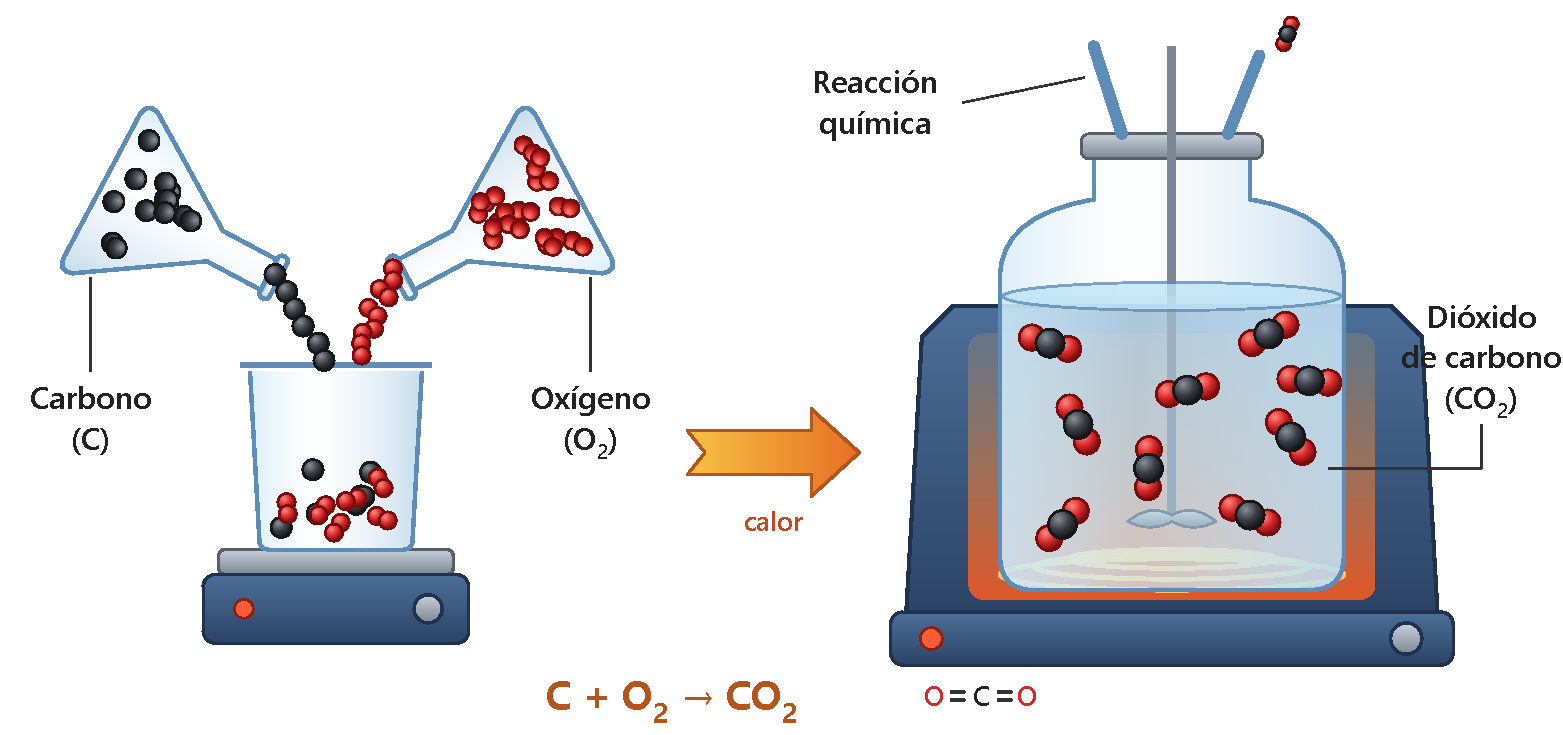
\includegraphics[width=\textwidth]{Figuras_SVG_ES/pdf/U8_reaccion_carbono_oxigeno.pdf}
    \caption{Reacción química}
    \label{fig:reaccion_quimica}
\end{figure}

\subsection{Cómo leer una reacción química}

Es necesario saber cómo escribir una reacción química a partir de su descripción con palabras.
Para ello seguimos las siguientes reglas.
Imaginemos la siguiente reacción general:
\begin{reaction*}
    A \gas{} + B \sld{} -> C \lqd{} + D \aq{}
\end{reaction*}
Aquí, los reactivos son A y B, mientras que los productos son C y D.
\begin{enumerate}[label=\numberballmDarkTeal]
        \item Si los reactivos o compuestos están escritos con su nombre, primero debemos obtener su fórmula.
        \item Si aparece el símbolo \( + \) en los reactivos, se lee como "reacciona con". Por ejemplo, en la ecuación anterior podemos decir que A reacciona con B.
        \item El símbolo \( \rightarrow \) se lee como \textquote{para formar} o \textquote{para dar}.
        \item Si el símbolo \( + \) está en los productos, ese \( + \) se lee como \textquote{y}.
        En el caso anterior podemos decir que se obtienen C \textquote{y} D.
        \item Junto a A aparece \gas{}, junto a B aparece \sld{}, junto a C aparece \lqd{}, mientras que junto a D aparece \aq{}. Estas palabras indican el estado de la materia de cada compuesto y tienen el siguiente significado:
        \begin{itemize}
            \item \sld{}: sólido.
            \item \lqd{}: líquido.
            \item \gas{}: gas.
            \item \aq{}: acuoso
        \end{itemize}
\end{enumerate}

\subsection{Cómo ocurre una reacción química}

Para que ocurra una reacción química, se deben seguir los siguientes pasos:
\begin{enumerate}[label=\numberballmDarkTeal]
        \item Los átomos de las moléculas reactivas deben separarse.
        \item Una vez separados los átomos, estos colisionan entre sí.
        Según la \negsubro{teoría de colisiones}, las reacciones químicas ocurren debido a colisiones entre átomos.
        Para que una colisión sea eficaz y produzca una reacción química, se debe cumplir lo siguiente:
        \begin{itemize}
            \item Los reactivos deben tener suficiente energía.
            \item Los reactivos deben colisionar con la orientación adecuada.
        \end{itemize}
        \item Una vez que ocurre una colisión eficaz, se obtienen los productos correspondientes.

        \begin{figure}[H]
            \centering
%            \includegraphics[scale=0.18]{images/reacciones_quimicas/reaccion_quimica_proceso_gemini}
            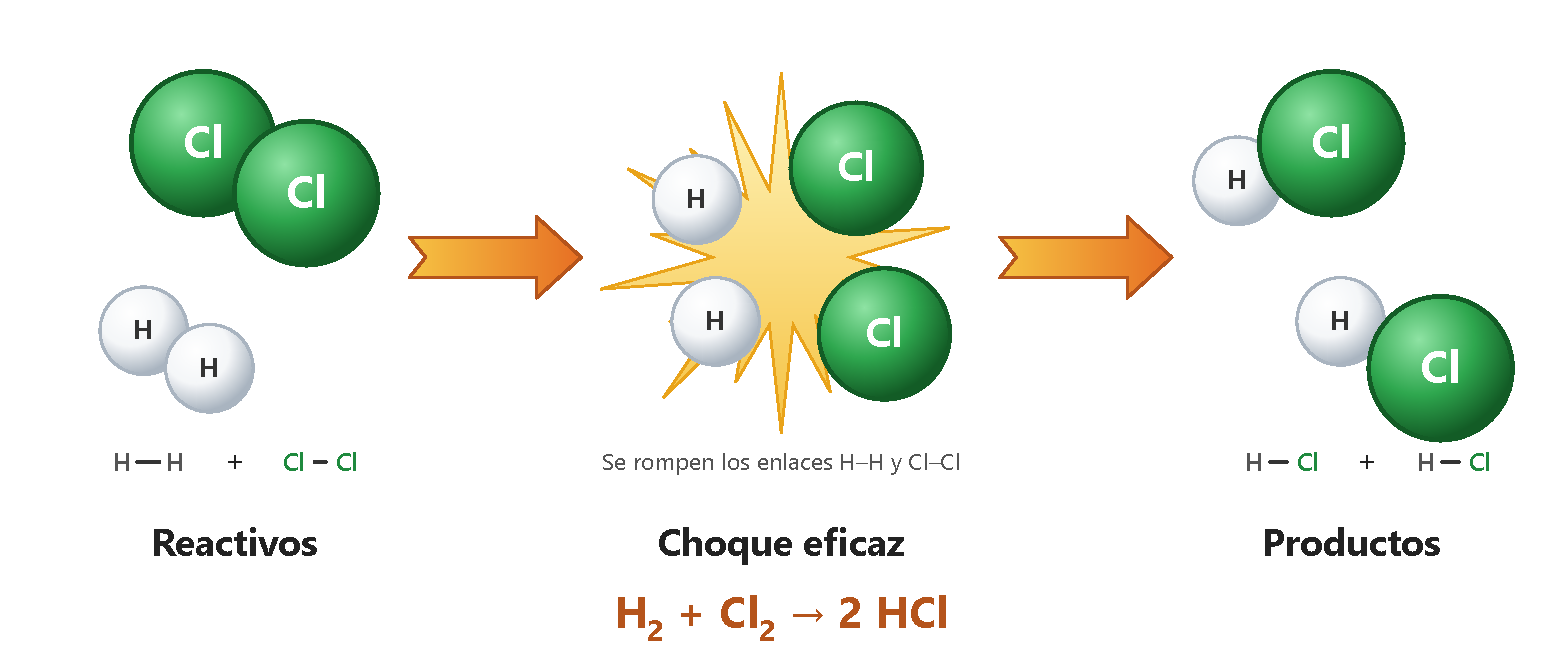
\includegraphics[width=0.95\textwidth]{Figuras_SVG_ES/pdf/U8_reaccion_proceso_H2_Cl2.pdf}
            \caption{}
            \label{fig:reaccion_quimica_proceso}
        \end{figure}
\end{enumerate}

%        Página xxx. Ejercicios 2 y 3.
%        \begin{exercise}{}
%            \begin{solu}{\arabic{ejercicionumero}}
%            \end{solu}
%        \end{exercise}

\begin{exercise}
    Cu representa el elemento cobre, S el elemento azufre y CuS el sulfuro de cobre(II). Usa tus propias palabras para explicar qué representa esta
    ecuación química
    \begin{solu}{\arabic{ejercicionumero}}
        Cu representa el elemento cobre, S el elemento azufre y CuS el sulfuro de cobre(II). Usa tus propias palabras para explicar qué representa esta
    ecuación química:

        El azufre reacciona con el cobre para formar sulfuro
        de cobre (II). En concreto, un átomo de azufre reacciona con un
        átomo de cobre para formar sulfuro de cobre (II).
    \end{solu}
\end{exercise}

\begin{exercise}
    El carbonato de calcio (CaCO3) se descompone a
    altas temperaturas en óxido de calcio (CaO) y
    dióxido de carbono (CO2). Este proceso se conoce como
    calcinación. Escribe la ecuación química para esta
    reacción.
    \begin{solu}{\arabic{ejercicionumero}}
         El carbonato de calcio (CaCO3) se descompone a altas temperaturas en óxido de calcio (CaO) y dióxido de carbono (CO2). Este proceso se conoce como calcinación. Escribe la ecuación química para esta reacción.

        \begin{reaction*}
            CaCO3\sld{} → CaO\sld{} + CO2\gas{}
        \end{reaction*}
    \end{solu}
\end{exercise}

\begin{exercise}
    ¿Cómo se llama la teoría que explica cómo ocurren las reacciones químicas?
    \begin{solu}{\arabic{ejercicionumero}}
         ¿Cómo se llama la teoría que explica cómo ocurren las reacciones químicas?

        Teoría de colisiones
    \end{solu}
\end{exercise}

\begin{exercise}
    Explica con palabras las siguientes ecuaciones químicas:
    \begin{reaction*}
        CuCO3\sld{} -> CUO\sld{} + CO2\gas{}
    \end{reaction*}
    \begin{reaction*}
        H2\gas{} + O2\gas{} ->  H2O\lqd{}
    \end{reaction*}
    \begin{solu}
         Explica con palabras las siguientes ecuaciones químicas:
    \begin{reaction*}
        CuCO3\sld{} -> CUO\sld{} + CO2\gas{}
    \end{reaction*}
    \begin{reaction*}
        H2\gas{} + O2\gas{} ->  H2O\lqd{}
    \end{reaction*}


        El carbonato de cobre (II) se descompone al calentarse
        para dar óxido de cobre (II) sólido y dióxido de
        carbono gaseoso.
        El hidrógeno gaseoso reacciona con oxígeno gaseoso
        para formar agua en estado líquido. En concreto, dos
        moléculas de hidrógeno reaccionan con una molécula de
        oxígeno para dar
        dos moléculas de agua.
        El ácido clorhídrico acuoso reacciona con hidróxido
        de sodio acuoso para dar cloruro de sodio acuoso
        y agua.
    \end{solu}
\end{exercise}


\section{Principio de Lavoisier. Ley de conservación de la masa}

En una reacción química (en un recipiente cerrado) la suma de las masas de los reactivos debe ser igual a la suma de las masas de los productos, es decir, \negsubro{la masa se conserva}.

Consideremos la siguiente reacción:
\begin{reaction*}
    AgNO3 + HCl -> AgCl + HNO3
\end{reaction*}
Si tenemos \qty{17}{\g} de \ch{AgNO3} y reacciona con \qty{3.65}{\g} de \ch{HCl}, se formarán \qty{14.35}{\g} de \ch{AgCl} y \qty{6.3}{\g} de \ch{HNO3}.
\begin{figure}[H]
    \centering
%    \includegraphics[scale=0.2]{images/reacciones_quimicas/conservacion_masa_EN}
    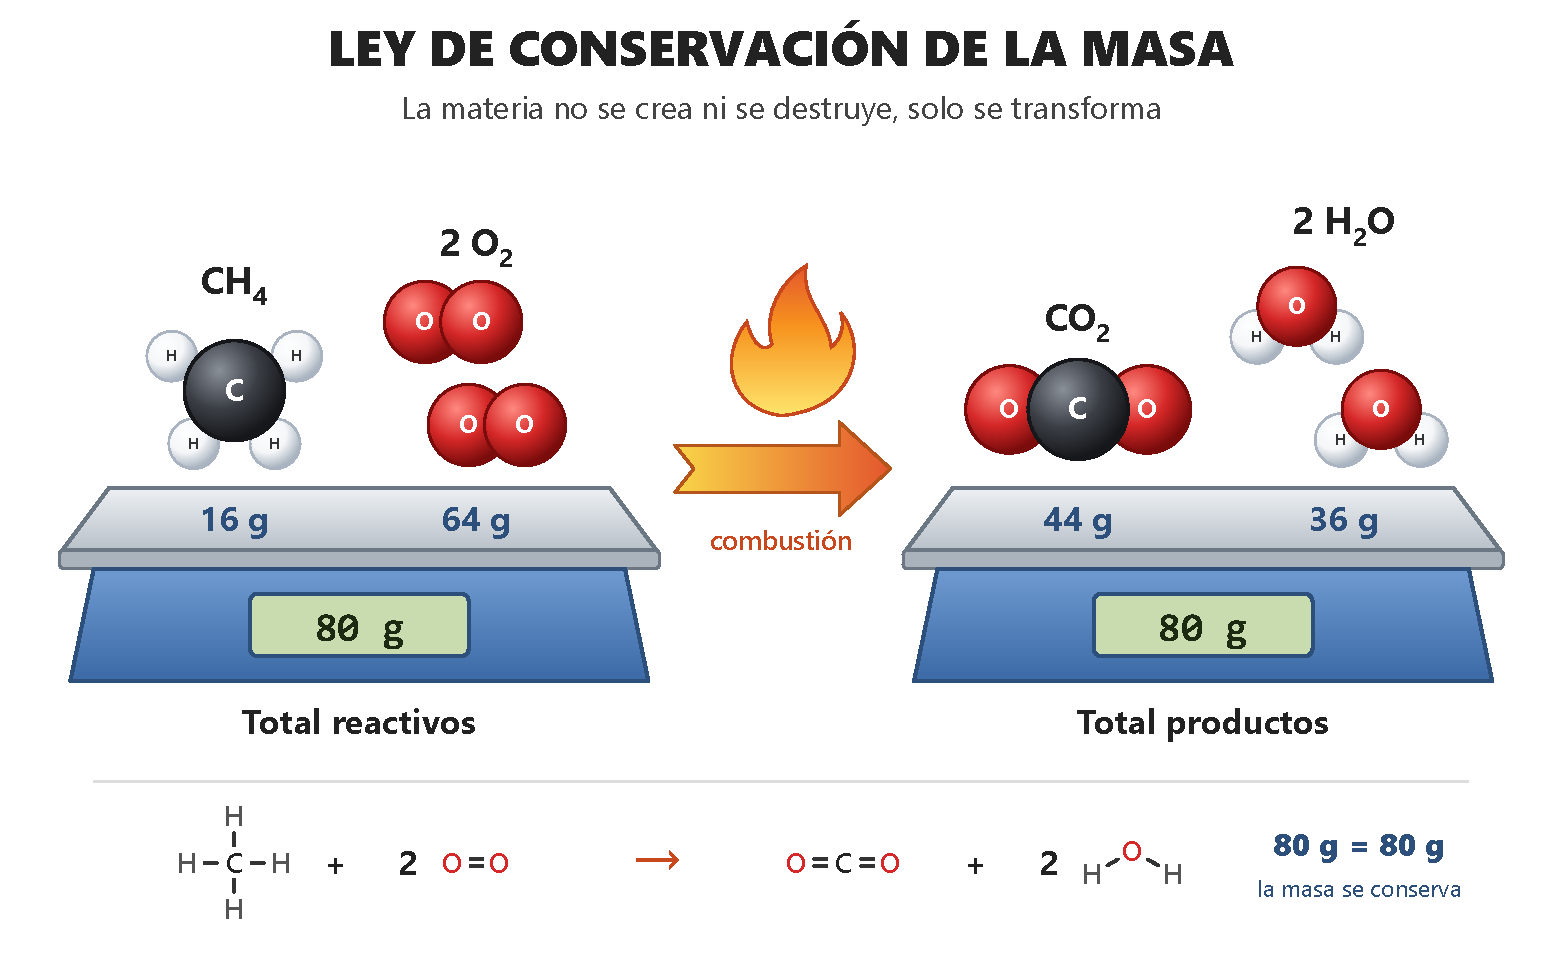
\includegraphics[width=0.9\textwidth]{Figuras_SVG_ES/pdf/U8_conservacion_masa.pdf}
    \caption{Ley de conservación de la masa}
    \label{fig:conservacion_masa}
\end{figure}

\subsection{Las reacciones químicas y la ley de conservación de la masa}

Toda reacción química debe cumplir el principio de Lavoisier y, por lo tanto:

\begin{displayquote}
    Debemos tener el mismo número de átomos de cada elemento en los reactivos (lado izquierdo) y en los productos (lado derecho).
    Cuando se da esta situación decimos que la reacción está \textbf{ajustada}
\end{displayquote}

Si la reacción química no está ajustada, debemos ajustarla para que se cumpla el principio de Lavoisier.

Los números colocados delante de cada fórmula química se conocen como \negsubro{coeficientes estequiométricos}.
\vspace*{12pt}
%
%    \begin{equation*}
%        \eqnmarkbox[blue]{hidrogeno}{\ch{2}}
%        \ch{H2 + }
%        \eqnmarkbox[violet]{oxigeno}{\ch{1}}
%        \ch{O2 ->}
%        \eqnmarkbox[red]{agua}{\ch{2}}
%        \ch{H2O}
%    \end{equation*}
%
%    \annotate[yshift=-2em]{below}{hidrogeno}{Coef. estequiométrico del \ch{H2}}
%    \annotate[yshift=-3.5em]{below}{oxigeno}{Coef. estequiométrico del \ch{O2}}
%    \annotate[yshift=-2em]{below}{agua}{Coef. estequiométrico del \ch{H2O}}
%
%\annotate[yshift=1em]{left}{node1}{Presión}
%    \annotate[yshift=-0.5em]{below,left}{volumen}{Volumen}
%    \annotate[yshift=1em]{}{moles}{número de moles}
%    \annotate[yshift=-2em]{below,left}{constante}{Constante de los gases ideales}
%    \annotate[yshift=-1em]{below}{temperatura}{Temperatura}
%
\begin{centeredequation}
    \eqnmarkbox[blue]{coehidrogeno}{\ch{2}}
    \tikzmarknode{reaccion}{\ch{H2 + O2 ->}}
    \eqnmarkbox[red]{coeagua}{\ch{2}}
    \ch{H2O}
\end{centeredequation}
%\begin{equation*}
%    \eqnmarkbox[blue]{coehidrogeno}{\ch{2}}
%    \tikzmarknode{reaccion}{\ch{H2 + O2 ->}}
%    \eqnmarkbox[red]{coeagua}{\ch{2}}
%    \ch{H2O}
%    %\tikzmarknode{node4}{\ch{H2O}}
%\end{equation*}
\vspace{8pt}
\annotate[yshift=1em]{}{coehidrogeno,coeagua}{Coeficientes estequiométricos}

%    \begin{figure}[H]
%        \centering
%        \includegraphics[scale=1]{images/unidad_5_imagenes/coeficientes_estequiometricos}
%        \caption{}
%        \label{fig:stechiometric_coefficients}
%    \end{figure}
Estos coeficientes estequiométricos nos indican el número de moléculas o moles de cada compuesto que reaccionan entre sí para obtener el número correspondiente de moléculas o moles de productos.

%    Por ejemplo, sea la reacción:
%    \begin{reaction*}
%        2 H2 + O2 -> 2 H2O
%    \end{reaction*}

%    Como podemos ver está ajustada.
Estos coeficientes estequiométricos nos indican que:
\begin{itemize}
    \item \negsubro{¡¡¡¡IMPORTANTE!!!!}: no aparece ningún número delante de \ch{O2}, cuando no tenemos un número debemos suponer que es un \( 1 \). Esto significa que reaccionará 1 mol de \ch{O2}.
    \item 2 moléculas de hidrógeno (\ch{H2}) reaccionan con 1 molécula de oxígeno (\ch{O2}) para formar 2 moléculas de agua (\ch{H2O}).
    \item 2 moles de hidrógeno (\ch{H2}) reaccionan con 1 mol de oxígeno (\ch{O2}) para formar 2 moles de agua (\ch{H2O}).
    \item Estos coeficientes también nos indican que 2 moles de \ch{H2} están relacionados con 1 mol de \ch{O2} y a su vez con 2 moles de \ch{H2O}.

\end{itemize}

\subsection{Pasos para el ajuste (Método de tanteo)}

\begin{enumerate}
    \item \textbf{Contar:} Contar los átomos de cada elemento en ambos lados de la flecha.
    \item \textbf{Ajustar con coeficientes:} Colocar números grandes delante de las moléculas para multiplicar el número de átomos.
    \item \textbf{Orden recomendado:}
    \begin{itemize}
        \item Metales y no metales.
        \item Hidrógeno ($H$).
        \item Oxígeno ($O$).
    \end{itemize}
\end{enumerate}

\paragraph{Ejemplo paso a paso: combustión del metano}

Queremos ajustar la siguiente reacción:
\[ \ch{CH4 + O2 -> CO2 + H2O} \]

        {\noindent  \textbf{Paso 1: Contar los átomos iniciales}}

\begin{itemize}
    \item Reactivos: $C=1, H=4, O=2$
    \item Productos: $C=1, H=2, O=3$ (2 del \ch{CO2} y 1 del \ch{H2O})
\end{itemize}

        {\noindent \textbf{Paso 2: Ajustar el hidrógeno}}

Como hay 4 $H$ en el lado izquierdo y solo 2 en el derecho, colocamos un \textbf{2} delante del agua:
\[ \ch{CH4 + O2 -> CO2 + 2 H2O} \]
Ahora tenemos: $H = 2 \times 2 = 4$. ¡Ajustado!

        {\noindent \textbf{Paso 3: Ajustar el oxígeno}}

Ahora en el lado derecho hay: 2 (del \ch{CO2}) + 2 (de \ch{2 H2O}) = 4 átomos de $O$.
En el lado izquierdo solo hay 2. Colocamos un \textbf{2} delante de \ch{O2}:
\[ \ch{CH4 + 2 O2 -> CO2 + 2 H2O} \]

        {\noindent \textbf{Resultado final}} La ecuación ajustada es:
\[ \mathbf{\ch{CH4 + 2 O2 -> CO2 + 2 H2O}} \]


\begin{exercise}
    En tu cuaderno, ajusta las ecuaciones químicas.
    \begin{multicols}{2}
        \begin{enumerate}[label=\letraminuscula]
            \item
            \begin{reaction*}
                Na\sld{} + O2\gas{}  → Na2O2\sld{}
            \end{reaction*}
            \item
            \begin{reaction*}
                H2 \gas{} + Cl2\gas{} → HCl\gas{}
            \end{reaction*}
            \item
            \begin{reaction*}
                Ca\sld{} + O2\gas{} → CaO\sld{}
            \end{reaction*}
            \item
            \begin{reaction*}
                Al\sld{} + Br2\lqd{} → AlBr3\sld{}
            \end{reaction*}
        \end{enumerate}
    \end{multicols}
    \begin{solu}
        \begin{enumerate}[label=\letraminuscula]
            \item
            \begin{reaction*}
                4 Na(s) + 2 O2(g) → 2 Na2O2(s)
            \end{reaction*}
            \item
            \begin{reaction*}
                2 H2(g) + 2 Cl2(g) → 4 HCl(g)
            \end{reaction*}
            \item
            \begin{reaction*}
                2 Ca(s) + O2(g) → 2 CaO(s)
            \end{reaction*}
            \item
            \begin{reaction*}
                2 Al(s) + 3 Br2(l) → 2 AlBr3(s)
            \end{reaction*}
        \end{enumerate}
    \end{solu}
\end{exercise}

\begin{exercise}
    Explica cómo se ajustan las ecuaciones químicas
    %\marcador{interesante para explicar como se ajustan las reacciones químicas.}
    \begin{solu}
        ¿Cómo ajustamos las ecuaciones químicas? Primero,
        identificamos los reactivos, las sustancias del
        lado izquierdo de la ecuación, y los productos, las
        sustancias del lado derecho de la ecuación.
        Después, contamos el número total de átomos de cada
        elemento en ambos lados de la ecuación. Si no son
        iguales en ambos lados entonces la ecuación no está
        ajustada.
        Para ajustar una ecuación química solo podemos cambiar
        los coeficientes. Los subíndices no se pueden cambiar.
        Después de haber cambiado los coeficientes, para ajustar
        tu ecuación cuenta de nuevo el número total de átomos de
        cada elemento y asegúrate de que el número total en
        ambos lados es igual. Si lo es, ahora tienes
        una ecuación química ajustada.
        a. Para ajustar una ecuación química, podemos cambiar
        el coeficiente pero nunca los subíndices.
        b. Tendremos una ecuación ajustada si el número
        total de átomos de un elemento dado es el
        mismo en ambos lados de la ecuación.
    \end{solu}
\end{exercise}

\begin{exercise}
    El hidrógeno reacciona con el oxígeno para dar agua. ¿Qué masa de agua líquida se obtiene si \qty{2}{\g} de hidrógeno reacciona exactamente con \qty{16}{\g} de oxígeno?
    \begin{solu}
        A partir de la ley de conservación de la masa, sabemos que se formarán \qty{18}{\g} de agua.
    \end{solu}
\end{exercise}

\begin{exercise}
    Hacemos reaccionar hierro con azufre para obtener sulfuro de hierro:
    \begin{reaction*}
        S (s) + Fe (s) → FeS (s)
    \end{reaction*}
    Sabemos que 32 g de azufre reaccionan exactamente con
    56 g de hierro.
    \begin{enumerate}[label=\letraminuscula]
            \item ¿Qué masa de sulfuro de hierro se obtiene?
            \item ¿Cuál es el porcentaje de azufre y hierro en el
            sulfuro de hierro?
    \end{enumerate}
    \begin{solu}
        \begin{enumerate}[label=\letraminuscula]
                \item Si reaccionan las masas exactas del enunciado,
                producirán 32 g + 56 g = 88 g de sulfuro
                de hierro.
                \item 32 g de S / 88 g de FeS = 36,36\% de S
                56 g de Fe / 88 g de FeS = 63,64\% de Fe
        \end{enumerate}
    \end{solu}
\end{exercise}

\begin{exercise}
    En un experimento, comprobamos que 3,2 g de azufre
    (S) reacciona completamente con 20 g de mercurio (Hg) para dar
    sulfuro de mercurio (II) (HgS). Ajusta la reacción
    y realiza los cálculos para las preguntas siguientes.
    \begin{reaction*}
        S (s) + Hg (l) → HgS (s)
    \end{reaction*}
    \begin{enumerate}[label=\letraminuscula]
            \item la cantidad de sulfuro de mercurio obtenida.
            \item la masa de azufre necesaria para reaccionar completamente con
            5 g de mercurio.
            \item la masa de mercurio necesaria para reaccionar completamente con
            10 g de azufre.
            \item el porcentaje de azufre y mercurio en el
            sulfuro de mercurio (II).
    \end{enumerate}
    \begin{solu}{\arabic{ejercicionumero}}

        \begin{enumerate}[label=\letraminuscula]
                \item Si reaccionan las masas exactas del enunciado,
                producirán 3,2 g + 20 g = 23,2 g de sulfuro
                de hierro.
                \item A partir de la relación entre las masas
                de azufre y mercurio que reaccionan para formar
                sulfuro de mercurio, la masa debe ser:
                3,2 g de S / 20 g de Hg = x g de S / 5 g de Hg;
                x = 0,8 g de S
                \item 3,2 g de S / 20 g de Hg = 10 g de S / x g de Hg;
                x = 62,5 g de Hg
                \item 3,2 g de S / 23,2 g de HgS = 13,8\% de S
                20 g de Hg / 23,2 g de HgS = 86,2\% de Hg
        \end{enumerate}
    \end{solu}
\end{exercise}

\begin{exercise}
    Escribe la ecuación química de la reacción del
    magnesio sólido con cloruro de hidrógeno (HCl)
    en disolución acuosa para dar cloruro de magnesio
    sólido (MgCl2) e hidrógeno gaseoso (H2). Ajusta
    la ecuación química.
    \begin{solu}

        La reacción es la siguiente:

        Mg (s) + HCl (aq) → MgCl2 (s) + H2 (g)
        2 Mg (s) + 2 HCl (aq) → 2 MgCl2 (s) + H2 (g)
    \end{solu}
\end{exercise}

\begin{exercise}
    Ajusta estas reacciones.
    \begin{enumerate}[label=\letraminuscula]
            \item Ca (s) + O2 (g) → CaO (s)
            \item CuO (s) + C (s) → Cu (s) + CO2 (g)
            \item Na (s) + Cl2 (g) → NaCl (s)
            \item Al (s) + O2 (g) → Al2O3 (s)
            \item Fe (s) + O2 (g) → FeO (s)
    \end{enumerate}
    \begin{solu}
        \begin{enumerate}[label=\letraminuscula]
                \item 2 Ca (s) + O2 (g) → 2 CaO (s)
                \item 2 CuO (s) + C (s) → 2 Cu (s) + CO2 (g)
                \item 2 Na (s) + Cl2 (g) → 2 NaCl (s)
                \item 4 Al (s) + 3 O2 (g) → 2 Al2O3 (s)
                \item 2 Fe (s) + O2 (g) → 2 FeO (s)a
        \end{enumerate}
    \end{solu}
\end{exercise}


\section{Cálculos con reacciones químicas}

Los cálculos en reacciones químicas nos permitirán saber qué cantidad (ya sea en gramos o moles) de productos se obtendrá o qué cantidad de reactivos necesitaremos.
Como ejemplo utilizaremos la reacción: el hidrógeno reacciona con el oxígeno para formar agua.

Para realizar los cálculos correctamente, se deben seguir los siguientes pasos:
\begin{enumerate}[label=\numberballmDarkTeal]
        \item Identificar los reactivos y productos.
        En este caso los reactivos serán \ch{H2} y \ch{O2} mientras que tendremos un único producto que es \ch{H2O}.
        \item Si en la reacción dicen hidrógeno, nitrógeno, oxígeno, flúor, cloro, bromo o yodo, siempre los escribiremos como \ch{H2}, \ch{N2}, \ch{O2}, \ch{F2}, \ch{Cl2}, \ch{Br2}, o \ch{I2}.
        También pueden nombrarse como nitrógeno molecular o dinitrógeno.
        Para el resto de los elementos mencionados anteriormente es lo mismo.
        \item Escribir la reacción química utilizando sus fórmulas químicas correspondientes.
        \begin{reaction*}
            H2 + O2 -> H2O
        \end{reaction*}
        \item Ajustar la reacción química si es necesario.
        \begin{reaction*}
            2 H2 + O2 -> 2 H2O
        \end{reaction*}
        \item Si nos dan cantidades en gramos, debemos convertirlas todas a moles (representaremos los moles con la letra \( \bm{n} \)).
        Si nos dan por ejemplo \qty{10}{\g} de \ch{H2O}, tendríamos que calcular primero la masa molar del agua que en este caso es \qty{18}{\g\per\mol}
        \begin{itemize}
            \item Usando la fórmula:
            \begin{equation*}
                n_{\ch{H2O}} = \dfrac{\text{gramos de sustancia}}{\text{masa molar del compuesto}} = \dfrac{\qty{10}{\g}}{\qty{18}{\g\per\mol}} = \qty{0.56}{\mol}\ \text{de \ch{H2O}}
            \end{equation*}
            \item También podemos usar factores de conversión:
            \begin{equation*}
                10\ \cancelred{\unit{\g}\ \text{de \ch{H2O}}} \cdot \dfrac{\qty{1}{\mol}\ \text{de \ch{H2O}}}{18\ \cancelred{\unit{\g} \ \text{de \ch{H2O}}}} = \qty{0.56}{\mol}\ \text{de \ch{H2O}}
            \end{equation*}
        \end{itemize}
        \item Ahora calculamos los moles necesarios para el resto de los compuestos utilizando los coeficientes estequiométricos.
        Ahora calcularemos los moles de \ch{H2} y \ch{O2}:

        Cálculo de los moles de \ch{H2}
        \begin{equation*}
            0.56\ \cancelred{\unit{\mol}\ \text{de \ch{H2O}}} \cdot \dfrac{\qty{2}{\mol}\ \text{de \ch{H2}}}{1\ \cancelred{\unit{\mol} \ \text{de \ch{H2O}}}} = \qty{1.12}{\mol}\ \text{de \ch{H2}}
        \end{equation*}
        Cálculo de los moles de \ch{O2}
        \begin{equation*}
            0.56\ \cancelred{\unit{\mol}\ \text{de \ch{H2O}}} \cdot \dfrac{\qty{1}{\mol}\ \text{de \ch{O2}}}{2\ \cancelred{\unit{\mol} \ \text{de \ch{H2O}}}} = \qty{0.28}{\mol}\ \text{de \ch{O2}}
        \end{equation*}
        \item Ahora calculamos en gramos las cantidades de todos esos compuestos solicitados

        Imaginemos ahora que calculamos la cantidad en gramos de \ch{H2} y \ch{O2}.
        Para ello usaremos los moles calculados anteriormente y la masa molar de cada compuesto.

        Cálculo de las masas molares:
        \begin{itemize}
            \item \ch{H2}: \( 2 \times 1 \text{ uma} = \qty{2}{\uma} =  \qty{2}{\g\per\mol} \)
            \item \ch{O2}: \( 2 \times 16 \text{ uma} = \qty{32}{\uma} = \qty{32}{\g\per\mol} \)
        \end{itemize}

        Ahora realizamos los cálculos que mencionamos anteriormente, lo haremos de dos formas distintas (solo es necesaria una) usando la fórmula de los moles y factores de conversión.
        \begin{itemize}
            \item Cálculo de los gramos de \ch{H2} y \ch{O2} usando la fórmula:

            Sabemos que \( n = \dfrac{\text{gramos de compuesto}}{\text{masa molar del compuesto}} \)

            si despejamos los gramos del compuesto tendremos:

            \( \text{gramos de compuesto} = n\cdot \text{masa molar del compuesto} \)

            gramos de \ch{H2} = \( 1.12 \cdot 2 = \qty{2.24}{\g}\ \text{de \ch{H2}} \).

            gramos de \ch{O2} = \( 0.28 \cdot 32 = \qty{8.96}{\g}\ \text{de \ch{O2}} \).
            \item Cálculo de los gramos de \ch{H2} y \ch{O2} usando factores de conversión. Para esto partiremos ahora de los moles obtenidos de \ch{H2} y \ch{O2} calculados en el apartado anterior y usando las masas molares de cada compuesto.

            \textbf{Cantidad de \ch{H2}}:
            \begin{equation*}
                1.12\ \cancelred{\unit{\mol}\ \text{de \ch{H2}}} \cdot \dfrac{\qty{2}{\g}\ \text{de \ch{H2}}}{1\ \cancelred{\unit{\mol} \ \text{de \ch{H2}}}} = \qty{2.24}{\g}\ \text{de \ch{H2}}
            \end{equation*}

            \textbf{Cantidad de \ch{O2}}:
            \begin{equation*}
                0.28\ \cancelred{\unit{\mol}\ \text{de \ch{O2}}} \cdot \dfrac{\qty{32}{\g}\ \text{de \ch{H2}}}{1\ \cancelred{\unit{\mol} \ \text{de \ch{O2}}}} = \qty{0.96}{\g}\ \text{de \ch{HO}}
            \end{equation*}
        \end{itemize}
\end{enumerate}

\begin{example}

    Dos elementos como el azufre y el cobre reaccionan para formar sulfuro de cobre(II). ¿Qué masa de sulfuro de cobre(II) se obtiene si partimos de \qty{64}{\g} de azufre?
    ¿Qué cantidad en gramos de cobre necesitamos?

    \begin{enumerate}[label=\numberballmDarkTeal]
            \item Identificamos los reactivos y productos.
            En este caso, los reactivos son \ch{S} y \ch{Cu} mientras que el producto es \ch{CuS}.
            \item Escribimos la reacción química:
            \begin{reaction*}
                S + Cu -> Cu2S
            \end{reaction*}
            \item Ajustamos la reacción y sería:
            \begin{reaction*}
                S + 2 Cu -> Cu2S
            \end{reaction*}
            \item Ahora calculamos los moles de todas las cantidades que pide el ejercicio.
            \begin{equation*}
                64\ \cancelred{\unit{\g}\ \text{de \ch{S}}} \cdot \dfrac{\qty{1}{\mole}\ \text{de \ch{S}}}{32\ \cancelred{\unit{\g} \ \text{de \ch{S}}}} = \qty{2}{\mol}\ \text{de \ch{S}}
            \end{equation*}
            \item Como piden la cantidad de \ch{CuS} y \ch{Cu}, calculamos los moles de cada especie con cálculos estequiométricos.
            \begin{itemize}
                \item Para CuS:
                \begin{equation*}
                    2\ \cancelred{\unit{\mol}\ \text{de \ch{S}}} \cdot \dfrac{\qty{1}{\mole}\ \text{de \ch{CuS}}}{1\ \cancelred{\unit{\mole} \ \text{de \ch{S}}}} = \qty{2}{\mol}\ \text{de \ch{S}}
                \end{equation*}
                \item Para Cu:
                \begin{equation*}
                    2\ \cancelred{\unit{\mol}\ \text{de \ch{S}}} \cdot \dfrac{\qty{2}{\mole}\ \text{de \ch{Cu}}}{1\ \cancelred{\unit{\mole} \ \text{de \ch{S}}}} = \qty{4}{\mol}\ \text{de \ch{S}}
                \end{equation*}
            \end{itemize}
            \item Ahora calculamos las masas en gramos de cada especie solicitada.
            \begin{itemize}
                \item Para CuS:
                \begin{equation*}
                    2\ \cancelred{\unit{\mol}\ \text{de \ch{CuS}}} \cdot \dfrac{\qty{95.5}{\g}\ \text{de \ch{CuS}}}{1\ \cancelred{\unit{\mole} \ \text{de \ch{CuS}}}} = \qty{191}{\g}\ \text{de \ch{CuS}}
                \end{equation*}
                \item Para Cu:
                \begin{equation*}
                    4\ \cancelred{\unit{\mol}\ \text{de \ch{Cu}}} \cdot \dfrac{\qty{63.5}{\g}\ \text{de \ch{Cu}}}{1\ \cancelred{\unit{\mole} \ \text{de \ch{Cu}}}} = \qty{254}{\g}\ \text{de \ch{Cu}}
                \end{equation*}
            \end{itemize}
            Estos mismos cálculos se pueden hacer utilizando la fórmula
            \begin{equation*}
                n = \dfrac{\text{gramos}}{\text{masa molar}} \longrightarrow \text{gramos} = n \cdot \text{masa molar}
            \end{equation*}
            \begin{itemize}
                \item Para CuS:
                \begin{equation*}
                    \text{gramos de } \ch{CuS} = 2\cdot 95.5 = \qty{191}{\g}\ \text{de \ch{CuS}}
                \end{equation*}
                \item Para CuS:
                \begin{equation*}
                    \text{gramos de } \ch{Cu} = 4\cdot 63.5 = \qty{254}{\g}\ \text{de \ch{Cu}}
                \end{equation*}
            \end{itemize}
    \end{enumerate}
\end{example}



\begin{exercise}
    ¿Qué masa de hidrógeno se forma cuando 27 g de aluminio reaccionan con exceso de ácido clorhídrico (HCl) según la ecuación?
    \begin{reaction*}
        2 Al + 6 HCl → 2 AlCl3 + 3 H2
    \end{reaction*}

    \begin{solu}
        \qty{3}{\g}
    \end{solu}
\end{exercise}

\begin{exercise}
    El carbonato de calcio (CaCO3), o piedra caliza,
    se descompone a altas temperaturas en óxido
    de calcio (CaO), o cal, y dióxido de carbono,
    según esta ecuación:
    \begin{reaction*}
        CaCO3 (s) → CaO (s) + CO2 (g)
    \end{reaction*}
    Si calentamos 160 kg de carbonato de calcio,
    obtenemos 89,6 kg de óxido de calcio. ¿Qué masa de
    óxido de calcio obtendríamos a partir de 80 kg de
    carbonato?
    \begin{solu}
        \qty{44.8}{\kg}
    \end{solu}
\end{exercise}

\begin{exercise}
    Al calentar 0,5 g de hierro pulverizado bajo una corriente
    de cloro gaseoso se produce dicloruro de hierro
    según esta reacción:
    \begin{reaction*}
        Fe (s) + Cl2 (g) → FeCl2 (s)
    \end{reaction*}
    \begin{enumerate}[label=\letraminuscula]
        \item Calcula la masa de cloro consumida.
        \item Calcula la masa de dicloruro de hierro
        producida.
    \end{enumerate}
    \begin{solu}
        \begin{enumerate}[label=\letraminuscula]
            \item 0,64 g
            \item 1,14 g
        \end{enumerate}
    \end{solu}
\end{exercise}

\begin{exercise}
    Un gramo de cinc arde en el aire según la ecuación:
    \begin{reaction*}
        Zn (s) + O2 (g) → ZnO (s)
    \end{reaction*}
    \begin{enumerate}[label=\letraminuscula]
        \item Ajusta la ecuación química.
        \item ¿Cuánto oxígeno consume?
        \item ¿Cuánto óxido de cinc produce?
        \item ¿Qué porcentaje de óxido de cinc es cinc?
        \item ¿Se cumple la ley de conservación de la masa?
    \end{enumerate}
    \begin{solu}
        \begin{enumerate}[label=\letraminuscula]
            \item \begin{reaction*}
                      2 Zn (s) + O2 (g) → 2 ZnO (s)
            \end{reaction*}
            donde \( \ch{Zn} = \qty{130.8}{\g}; \ch{O2} = \qty{32}{\g}; \ch{ZnO} = \qty{162.8}{\g} \)
        \end{enumerate}
    \end{solu}
\end{exercise}

\begin{exercise}
    El mercurio y el azufre reaccionan para formar sulfuro de mercurio según esta fórmula:
    \begin{reaction*}
        S (s) + Hg (s) → HgS (s)
    \end{reaction*}
    Si reaccionan 20 g de Hg:
    \begin{enumerate}[label=\letraminuscula]
        \item ¿con cuánto azufre reacciona?
        \item ¿qué masa de sulfuro de mercurio
        produce?
    \end{enumerate}
    \begin{solu}

    \end{solu}
\end{exercise}

\begin{exercise}
    El magnesio (Mg) reacciona con oxígeno (O2) para dar óxido de magnesio (MgO).
    \begin{enumerate}[label=\letraminuscula]
        \item Escribe y ajusta esta ecuación química.
        \item Si 48,6 g de magnesio reaccionan con la
        cantidad necesaria de oxígeno, ¿cuánto
        óxido de magnesio se obtiene?
    \end{enumerate}
    \begin{solu}
        \begin{enumerate}[label=\letraminuscula]
            \item La ecuación ajustada es:
            \begin{reaction*}
                2Mg + O2 → 2MgO
            \end{reaction*}
            \item Escribimos la reacción y las masas involucradas:
            \begin{reaction*}
                2 Mg + O2 → 2 MgO
            \end{reaction*}
            \( \ch{Mg} = \qty{48.6}{\g}; \ch{O2} = \qty{32}{\g}; \ch{MgO} = \qty{80.6}{\g} \)

            Obtendríamos 80,6 g de MgO.
        \end{enumerate}
    \end{solu}
\end{exercise}


%
%    \section{Ideal Gas Law}
%
%    In a chemical reaction, it is advisable to know the state too atter to the compound, that is, whether it is a solid, a gas, or a liquid.
%    To indicate it in the chemical reaction, \gas{} is placed next to the compound for gases, \lqd{} and \sld{} for a solid.
%    An example could be:
%
%    \begin{reaction*}
%        O2\gas{} + C \sld{} -> CO2 \lqd{}
%    \end{reaction*}
%
%    For gases, the three gas laws (Gay-Lussac's Law, Charles's Law, and Boyle-Mariotte's Law) can be concentrated into one law known as the \textbf{Ideal Gas Law} and this law relates the magnitudes too ressure, volume, and temperature with the amount to substance expressed in moles.
%    The mathematical expression to this law will be:
%    \vspace{20pt}
%
%    \begin{equation*}
%        \eqnmarkbox[blue]{presion}{p}
%        \cdot
%        \eqnmarkbox[red]{volumen}{V}
%        =
%        \eqnmarkbox[mDarkTeal]{moles}{n}
%        \cdot
%        \eqnmarkbox[orange]{constante}{R}
%        \cdot
%        \eqnmarkbox[violet]{temperatura}{T}
%    \end{equation*}
%    \vspace{25pt}
%    \annotate[yshift=1em]{left}{presion}{Pressure}
%    \annotate[yshift=-0.5em]{below,left}{volumen}{Volume}
%    \annotate[yshift=1em]{}{moles}{number to moles}
%    \annotate[yshift=-2em]{below,left}{constante}{Ideal gas constant}
%    \annotate[yshift=-1em]{below}{temperatura}{Temperature}
%
%    where:
%    \begin{itemize}
%        \item \( p \) is the system pressure expressed in \unit{\atmosphere}.
%        \item \( V \) is the system volume expressed in \unit{\litre}.
%        \item \( R \) is a constant called the ideal gas constant and has a value  \( R = \ctegases{} \).
%        \item \( T \) is the system temperature expressed in \unit{\kelvin}.
%    \end{itemize}

%
%        \begin{exercise}{}
%            Aluminium reacts with oxygen producing aluminium oxide.
%            Calculate the mass to aluminium oxide produced when \qty{15}{\g} to aluminium reacts with excess oxygen.
%        \end{exercise}
%
%        \begin{exercise}{}
%            What is the volume in mL occupied by an ideal gas if \qty{0.553}{\mol} are at a temperature to \qty{1226.49}{\kelvin} and a pressure to \qty{4935}{\mmHg}?
%        \end{exercise}
%
%        \begin{exercise}{}
%            What is the temperature in \unit{\kelvin} to an ideal gas, if \qty{0.405}{\mole} occupy a volume to \qty{7720}{\mL} at a pressure to \qty{790}{\mmHg}?
%        \end{exercise}
%
%        \begin{exercise}{}
%            What is the temperature in \unit{\degreeCelsius} to an ideal gas, if \qty{0.746}{\mol} occupy a volume to \qty{9890}{\mL} at a pressure to \qty{1.41}{\atmosphere}?
%        \end{exercise}
%
%        \begin{exercise}{}
%            What is the pressure in atm to an ideal gas if \qty{0.532}{\mol} occupy a volume to \qty{4390}{\mL} at a temperature to \qty{183.93}{\kelvin}?
%        \end{exercise}
%
%        \begin{exercise}{}
%            How many moles to an ideal gas are in a volume too qty{4220}{\mL} if the temperature is \qty{279.35}{\kelvin} and the pressure is \qty{1.75}{\atmosphere}?
%        \end{exercise}
%
%        \begin{exercise}{}
%            How many moles to an ideal gas are in a volume too qty{9.37}{\litre} if the temperature is
%        \end{exercise}
%
%
%    \subsection{Standard conditions (STP)}
%
%    In chemistry, it is very common to talk about standard conditions.
%    When we talk about standard conditions we set the pressure at \qty{1}{\atmosphere} and the temperature at \qty{0}{\degreeCelsius}.
%
%    It is important to know that \qty{1}{\mol} to \textbf{any gas} always occupies a volume to \qty{22.4}{\litre}.
%
%    To verify this value, we just need to apply the ideal gas equation seen previously, setting \( n=1 \), \( p = \qty{1}{\atmosphere} \), and \( T = \qty{273}{\kelvin} \)


\begin{exercise}
    El aluminio reacciona con el oxígeno produciendo óxido de aluminio.
    Calcula la masa de óxido de aluminio producido cuando \qty{15}{\g} de aluminio reacciona con exceso de oxígeno.
    \begin{solu}
        \textbf{Paso 1: Escribir la ecuación química y ajustarla}

        La reacción entre el aluminio y el oxígeno es:
        \begin{equation*}
            \ch{Al + O2 -> Al2O3}
        \end{equation*}

        Ajustamos la ecuación:
        \begin{equation*}
            \ch{4 Al + 3 O2 -> 2 Al2O3}
        \end{equation*}

        \textbf{Paso 2: Calcular las masas molares}

        \begin{itemize}
            \item Masa molar de \ch{Al}: $M(\ch{Al}) = \qty{27}{\g\per\mol}$
            \item Masa molar de \ch{Al2O3}: $M(\ch{Al2O3}) = 2 \times 27 + 3 \times 16 = \qty{102}{\g\per\mol}$
        \end{itemize}

        \textbf{Paso 3: Calcular los moles de aluminio que reaccionan}

        Usamos la relación: $n = \dfrac{m}{M}$
        \begin{equation*}
            n(\ch{Al}) = \frac{15\,\text{g}}{27\,\text{g/mol}} = 0.556\,\text{mol}
        \end{equation*}

        \textbf{Paso 4: Aplicar la estequiometría}

        Según la ecuación ajustada: $4\,\text{mol de Al} \rightarrow 2\,\text{mol de \ch{Al2O3}}$

        Por lo tanto: $\dfrac{n(\ch{Al2O3})}{n(\ch{Al})} = \dfrac{2}{4} = \dfrac{1}{2}$

        \begin{equation*}
            n(\ch{Al2O3}) = 0.556 \times \frac{1}{2} = 0.278\,\text{mol}
        \end{equation*}

        \textbf{Paso 5: Calcular la masa de óxido de aluminio producida}

        Usamos: $m = n \times M$
        \begin{equation*}
            m(\ch{Al2O3}) = 0.278\,\text{mol} \times 102\,\text{g/mol} = \qty{28.36}{\g}
        \end{equation*}

        \textbf{Respuesta:} se producen \qty{28.36}{\g} de \ch{Al2O3}.
    \end{solu}
\end{exercise}

\begin{exercise}
    El aluminio reacciona con el oxígeno produciendo óxido de aluminio.
    Calcula la masa de óxido de aluminio producido cuando 15 g de aluminio reacciona con exceso de oxígeno.
    \begin{solu}
        \textbf{Paso 1: Escribir la ecuación química y ajustarla}

        La reacción entre el aluminio y el oxígeno es:
        \begin{equation*}
            \ch{Al + O2 -> Al2O3}
        \end{equation*}

        Ajustamos la ecuación:
        \begin{equation*}
            \ch{4 Al + 3 O2 -> 2 Al2O3}
        \end{equation*}

        \textbf{Paso 2: Calcular las masas molares}

        \begin{itemize}
            \item Masa molar de \ch{Al}: $M(\ch{Al}) = 27\,\text{g/mol}$
            \item Masa molar de \ch{Al2O3}: $M(\ch{Al2O3}) = 2 \times 27 + 3 \times 16 = 102\,\text{g/mol}$
        \end{itemize}

        \textbf{Paso 3: Calcular los moles de aluminio que reaccionan}

        Usamos la relación: $n = \dfrac{m}{M}$
        \begin{equation*}
            n(\ch{Al}) = \frac{15\,\text{g}}{27\,\text{g/mol}} = 0.556\,\text{mol}
        \end{equation*}

        \textbf{Paso 4: Aplicar la estequiometría}

        Según la ecuación ajustada: $4\,\text{mol de Al} \rightarrow 2\,\text{mol de \ch{Al2O3}}$

        Por lo tanto: $\dfrac{n(\ch{Al2O3})}{n(\ch{Al})} = \dfrac{2}{4} = \dfrac{1}{2}$

        \begin{equation*}
            n(\ch{Al2O3}) = 0.556 \times \frac{1}{2} = 0.278\,\text{mol}
        \end{equation*}

        \textbf{Paso 5: Calcular la masa de óxido de aluminio producida}

        Usamos: $m = n \times M$
        \begin{equation*}
            m(\ch{Al2O3}) = 0.278\,\text{mol} \times 102\,\text{g/mol} = 28.36\,\text{g}
        \end{equation*}

        \textbf{Respuesta:} se producen 28,36 g de \ch{Al2O3}.
    \end{solu}
\end{exercise}

\begin{exercise}
    El amoniaco (NH3) se forma por la reacción del nitrógeno con el hidrógeno.
    Si
    disponemos de 420 g de nitrógeno, ¿cuántos gramos de amoniaco se forman? ¿Qué volumen de
    hidrógeno en condiciones estándar se consume en la reacción?
    \begin{solu}
        \textbf{Paso 1: Escribir la ecuación química y ajustarla}

        La reacción de formación del amoniaco es:
        \begin{equation*}
            \ch{N2 + H2 -> NH3}
        \end{equation*}

        Ajustamos la ecuación:
        \begin{equation*}
            \ch{N2 + 3 H2 -> 2 NH3}
        \end{equation*}

        \textbf{Paso 2: Calcular las masas molares}

        \begin{itemize}
            \item Masa molar de \ch{N2}: $M(\ch{N2}) = 2 \times 14 = 28\,\text{g/mol}$
            \item Masa molar de \ch{NH3}: $M(\ch{NH3}) = 14 + 3 \times 1 = 17\,\text{g/mol}$
        \end{itemize}

        \textbf{Paso 3: Calcular los moles de nitrógeno disponibles}

        \begin{equation*}
            n(\ch{N2}) = \frac{420\,\text{g}}{28\,\text{g/mol}} = 15\,\text{mol}
        \end{equation*}

        \textbf{Paso 4: Calcular los moles de amoniaco que se forman}

        Según la ecuación: $1\,\text{mol de \ch{N2}} \rightarrow 2\,\text{mol de \ch{NH3}}$

        \begin{equation*}
            n(\ch{NH3}) = 15\,\text{mol} \times 2 = 30\,\text{mol}
        \end{equation*}

        \textbf{Paso 5: Calcular la masa de amoniaco producida}

        \begin{equation*}
            m(\ch{NH3}) = 30\,\text{mol} \times 17\,\text{g/mol} = 510\,\text{g}
        \end{equation*}

        \textbf{Paso 6: Calcular los moles de hidrógeno consumidos}

        Según la ecuación: $1\,\text{mol de \ch{N2}} \rightarrow 3\,\text{mol de \ch{H2}}$

        \begin{equation*}
            n(\ch{H2}) = 15\,\text{mol} \times 3 = 45\,\text{mol}
        \end{equation*}

        \textbf{Paso 7: Calcular el volumen de hidrógeno en condiciones estándar}

        En condiciones estándar: $V_m = 22.4\,\text{L/mol}$

        \begin{equation*}
            V(\ch{H2}) = 45\,\text{mol} \times 22.4\,\text{L/mol} = 1008\,\text{L}
        \end{equation*}

        \textbf{Respuesta:} se forman 510 g de \ch{NH3} y se consumen 1008 L de \ch{H2} en condiciones estándar.
    \end{solu}
\end{exercise}

\begin{exercise}
    El sulfuro de cinc reacciona con el oxígeno produciendo óxido de cinc y dióxido de azufre.
    Con 168 L de oxígeno en condiciones estándar:
    \begin{enumerate}[label=\letraminuscula]
    \item
    ¿qué masa de sulfuro de cinc reaccionará?
    \item
    ¿cuántos moles de óxido de cinc se producirán?
    \item
    ¿qué volumen de dióxido de azufre en condiciones estándar se obtendrá?
    \end{enumerate}
    \begin{solu}
        \textbf{Paso 1: Escribir la ecuación química y ajustarla}

        La reacción es:
        \begin{equation*}
            \ch{ZnS + O2 -> ZnO + SO2}
        \end{equation*}

        Ajustamos la ecuación:
        \begin{equation*}
            \ch{2 ZnS + 3 O2 -> 2 ZnO + 2 SO2}
        \end{equation*}

        \textbf{Paso 2: Calcular los moles de oxígeno disponibles}

        En condiciones estándar: $V_m = 22.4\,\text{L/mol}$

        \begin{equation*}
            n(\ch{O2}) = \frac{168\,\text{L}}{22.4\,\text{L/mol}} = 7.5\,\text{mol}
        \end{equation*}

        \textbf{Apartado a) Masa de sulfuro de cinc que reacciona}

        \textbf{Paso 3a: Calcular los moles de ZnS}

        Según la ecuación: $3\,\text{mol de \ch{O2}} \rightarrow 2\,\text{mol de \ch{ZnS}}$

        \begin{equation*}
            n(\ch{ZnS}) = 7.5\,\text{mol} \times \frac{2}{3} = 5\,\text{mol}
        \end{equation*}

        \textbf{Paso 4a: Calcular la masa de ZnS}

        Masa molar de \ch{ZnS}: $M(\ch{ZnS}) = 65 + 32 = 97\,\text{g/mol}$

        \begin{equation*}
            m(\ch{ZnS}) = 5\,\text{mol} \times 97\,\text{g/mol} = 485\,\text{g}
        \end{equation*}

        \textbf{Apartado b) Moles de óxido de cinc producidos}

        \textbf{Paso 3b: Aplicar la estequiometría}

        Según la ecuación: $3\,\text{mol de \ch{O2}} \rightarrow 2\,\text{mol de \ch{ZnO}}$

        \begin{equation*}
            n(\ch{ZnO}) = 7.5\,\text{mol} \times \frac{2}{3} = 5\,\text{mol}
        \end{equation*}

        \textbf{Apartado c) Volumen de dióxido de azufre en condiciones estándar}

        \textbf{Paso 3c: Calcular los moles de \ch{SO2}}

        Según la ecuación: $3\,\text{mol de \ch{O2}} \rightarrow 2\,\text{mol de \ch{SO2}}$

        \begin{equation*}
            n(\ch{SO2}) = 7.5\,\text{mol} \times \frac{2}{3} = 5\,\text{mol}
        \end{equation*}

        \textbf{Paso 4c: Calcular el volumen de \ch{SO2}}

        \begin{equation*}
            V(\ch{SO2}) = 5\,\text{mol} \times 22.4\,\text{L/mol} = 112\,\text{L}
        \end{equation*}

        \textbf{Respuestas:}
        \begin{enumerate}[label=\letraminuscula]
            \item reaccionan 485 g de \ch{ZnS}
            \item se producen 5 mol de \ch{ZnO}
            \item se obtienen 112 L de \ch{SO2} en condiciones estándar
        \end{enumerate}
    \end{solu}
\end{exercise}

\begin{exercise}
    El metano (\ch{CH4}) reacciona con el oxígeno produciendo dióxido de carbono y agua.
    Con \qty{20}{\mol} de metano:
    \begin{enumerate}[label=\letraminuscula]
    \item ¿qué volumen de oxígeno, en condiciones estándar, reacciona?
    \item ¿qué masa de dióxido de carbono se forma?
    ¿cuántos moles de agua se producen?
    \end{enumerate}
    \begin{solu}
        \textbf{Paso 1: Escribir la ecuación química y ajustarla}

        La reacción de combustión del metano es:
        \begin{equation*}
            \ch{CH4 + O2 -> CO2 + H2O}
        \end{equation*}

        Ajustamos la ecuación:
        \begin{equation*}
            \ch{CH4 + 2 O2 -> CO2 + 2 H2O}
        \end{equation*}

        \textbf{Apartado a) Volumen de oxígeno que reacciona}

        \textbf{Paso 2a: Calcular los moles de oxígeno necesarios}

        Según la ecuación: $1\,\text{mol de \ch{CH4}} \rightarrow 2\,\text{mol de \ch{O2}}$

        \begin{equation*}
            n(\ch{O2}) = 20\,\text{mol} \times 2 = 40\,\text{mol}
        \end{equation*}

        \textbf{Paso 3a: Calcular el volumen de oxígeno en condiciones estándar}

        En condiciones estándar: $V_m = 22.4\,\text{L/mol}$

        \begin{equation*}
            V(\ch{O2}) = 40\,\text{mol} \times 22.4\,\text{L/mol} = 896\,\text{L}
        \end{equation*}

        \textbf{Apartado b) Masa de dióxido de carbono que se forma}

        \textbf{Paso 2b: Calcular los moles de \ch{CO2}}

        Según la ecuación: $1\,\text{mol de \ch{CH4}} \rightarrow 1\,\text{mol de \ch{CO2}}$

        \begin{equation*}
            n(\ch{CO2}) = 20\,\text{mol} \times 1 = 20\,\text{mol}
        \end{equation*}

        \textbf{Paso 3b: Calcular la masa de \ch{CO2}}

        Masa molar de \ch{CO2}: $M(\ch{CO2}) = 12 + 2 \times 16 = 44\,\text{g/mol}$

        \begin{equation*}
            m(\ch{CO2}) = 20\,\text{mol} \times 44\,\text{g/mol} = 880\,\text{g}
        \end{equation*}

        \textbf{Apartado c) Moles de agua que se producen}

        \textbf{Paso 2c: Calcular los moles de \ch{H2O}}

        Según la ecuación: $1\,\text{mol de \ch{CH4}} \rightarrow 2\,\text{mol de \ch{H2O}}$

        \begin{equation*}
            n(\ch{H2O}) = 20\,\text{mol} \times 2 = 40\,\text{mol}
        \end{equation*}

        \textbf{Respuestas:}
        \begin{enumerate}[label=\letraminuscula]
            \item reaccionan 896 L de \ch{O2} en condiciones estándar
            \item se forman 880 g de \ch{CO2} y 40 mol de \ch{H2O}
        \end{enumerate}
    \end{solu}
\end{exercise}

\begin{exercise}
    Por efecto del calor, \qty{245}{\g} de clorato de potasio (\ch{KClO3}) se descomponen. Calcula la masa de KCl y los moles de oxígeno que se forman.
    \begin{solu}
        \textbf{Paso 1: Escribir la ecuación química y ajustarla}

        La descomposición térmica del clorato de potasio es:
        \begin{equation*}
            \ch{KClO3 -> KCl + O2}
        \end{equation*}

        Ajustamos la ecuación:
        \begin{equation*}
            \ch{2 KClO3 -> 2 KCl + 3 O2}
        \end{equation*}

        \textbf{Paso 2: Calcular las masas molares}

        \begin{itemize}
            \item Masa molar de \ch{KClO3}: $M(\ch{KClO3}) = 39 + 35.5 + 3 \times 16 = 122.5\,\text{g/mol}$
            \item Masa molar de \ch{KCl}: $M(\ch{KCl}) = 39 + 35.5 = 74.5\,\text{g/mol}$
        \end{itemize}

        \textbf{Paso 3: Calcular los moles de \ch{KClO3} que se descomponen}

        \begin{equation*}
            n(\ch{KClO3}) = \frac{245\,\text{g}}{122.5\,\text{g/mol}} = 2\,\text{mol}
        \end{equation*}

        \textbf{Paso 4: Calcular los moles de KCl que se forman}

        Según la ecuación: $2\,\text{mol de \ch{KClO3}} \rightarrow 2\,\text{mol de \ch{KCl}}$

        La proporción es 1:1, por lo tanto:
        \begin{equation*}
            n(\ch{KCl}) = 2\,\text{mol}
        \end{equation*}

        \textbf{Paso 5: Calcular la masa de KCl}

        \begin{equation*}
            m(\ch{KCl}) = 2\,\text{mol} \times 74.5\,\text{g/mol} = 149\,\text{g}
        \end{equation*}

        \textbf{Paso 6: Calcular los moles de oxígeno que se forman}

        Según la ecuación: $2\,\text{mol de \ch{KClO3}} \rightarrow 3\,\text{mol de \ch{O2}}$

        \begin{equation*}
            n(\ch{O2}) = 2\,\text{mol} \times \frac{3}{2} = 3\,\text{mol}
        \end{equation*}

        \textbf{Respuesta:} se forman 149 g de \ch{KCl} y 3 mol de \ch{O2}.
    \end{solu}
\end{exercise}

\begin{exercise}
    Calcula el volumen de dióxido de carbono (en condiciones estándar) y la masa de agua producidos en la combustión de 100 g de butano (C4H10).
    ¿Cuántos moles de oxígeno se consumen?
    \begin{solu}
        \textbf{Paso 1: Escribir la ecuación química y ajustarla}

        La reacción de combustión del butano es:
        \begin{equation*}
            \ch{C4H10 + O2 -> CO2 + H2O}
        \end{equation*}

        Ajustamos la ecuación:
        \begin{equation*}
            \ch{2 C4H10 + 13 O2 -> 8 CO2 + 10 H2O}
        \end{equation*}

        \textbf{Paso 2: Calcular la masa molar del butano}

        $M(\ch{C4H10}) = 4 \times 12 + 10 \times 1 = 58\,\text{g/mol}$

        \textbf{Paso 3: Calcular los moles de butano que arden}

        \begin{equation*}
            n(\ch{C4H10}) = \frac{100\,\text{g}}{58\,\text{g/mol}} = 1.724\,\text{mol}
        \end{equation*}

        \textbf{Paso 4: Calcular los moles de \ch{CO2} que se forman}

        Según la ecuación: $2\,\text{mol de \ch{C4H10}} \rightarrow 8\,\text{mol de \ch{CO2}}$

        Por lo tanto: $\dfrac{n(\ch{CO2})}{n(\ch{C4H10})} = \dfrac{8}{2} = 4$

        \begin{equation*}
            n(\ch{CO2}) = 1.724\,\text{mol} \times 4 = 6.896\,\text{mol}
        \end{equation*}

        \textbf{Paso 5: Calcular el volumen de \ch{CO2} en condiciones estándar}

        \begin{equation*}
            V(\ch{CO2}) = 6.896\,\text{mol} \times 22.4\,\text{L/mol} = 154.47\,\text{L}
        \end{equation*}

        \textbf{Paso 6: Calcular los moles de \ch{H2O} que se forman}

        Según la ecuación: $2\,\text{mol de \ch{C4H10}} \rightarrow 10\,\text{mol de \ch{H2O}}$

        Por lo tanto: $\dfrac{n(\ch{H2O})}{n(\ch{C4H10})} = \dfrac{10}{2} = 5$

        \begin{equation*}
            n(\ch{H2O}) = 1.724\,\text{mol} \times 5 = 8.62\,\text{mol}
        \end{equation*}

        \textbf{Paso 7: Calcular la masa de \ch{H2O}}

        Masa molar de \ch{H2O}: $M(\ch{H2O}) = 2 \times 1 + 16 = 18\,\text{g/mol}$

        \begin{equation*}
            m(\ch{H2O}) = 8.62\,\text{mol} \times 18\,\text{g/mol} = 155.16\,\text{g}
        \end{equation*}

        \textbf{Paso 8: Calcular los moles de \ch{O2} consumidos}

        Según la ecuación: $2\,\text{mol de \ch{C4H10}} \rightarrow 13\,\text{mol de \ch{O2}}$

        Por lo tanto: $\dfrac{n(\ch{O2})}{n(\ch{C4H10})} = \dfrac{13}{2} = 6.5$

        \begin{equation*}
            n(\ch{O2}) = 1.724\,\text{mol} \times 6.5 = 11.206\,\text{mol}
        \end{equation*}

        \textbf{Respuesta:} 154,47 L de \ch{CO2} en condiciones estándar, se producen 155,16 g de \ch{H2O}, y se consumen 11,21 mol de \ch{O2}.
    \end{solu}
\end{exercise}

\begin{exercise}
    El amoniaco (NH3) reacciona con el oxígeno produciendo monóxido de nitrógeno y agua. Si
    se han obtenido 500 cm³ de monóxido de nitrógeno, medidos en condiciones estándar,
    ¿cuántos gramos de amoniaco y cuántos moles de oxígeno se habrán consumido?
    \begin{solu}
        \textbf{Paso 1: Escribir la ecuación química y ajustarla}

        La reacción es:
        \begin{equation*}
            \ch{NH3 + O2 -> NO + H2O}
        \end{equation*}

        Ajustamos la ecuación:
        \begin{equation*}
            \ch{4 NH3 + 5 O2 -> 4 NO + 6 H2O}
        \end{equation*}

        \textbf{Paso 2: Convertir el volumen de NO a litros}

        \begin{equation*}
            V(\ch{NO}) = 500\,\text{cm}^3 = 0.5\,\text{L}
        \end{equation*}

        \textbf{Paso 3: Calcular los moles de NO producidos}

        En condiciones estándar: $V_m = 22.4\,\text{L/mol}$

        \begin{equation*}
            n(\ch{NO}) = \frac{0.5\,\text{L}}{22.4\,\text{L/mol}} = 0.0223\,\text{mol}
        \end{equation*}

        \textbf{Paso 4: Calcular los moles de \ch{NH3} consumidos}

        Según la ecuación: $4\,\text{mol de \ch{NH3}} \rightarrow 4\,\text{mol de \ch{NO}}$

        La proporción es 1:1, por lo tanto:
        \begin{equation*}
            n(\ch{NH3}) = 0.0223\,\text{mol}
        \end{equation*}

        \textbf{Paso 5: Calcular la masa de \ch{NH3}}

        Masa molar de \ch{NH3}: $M(\ch{NH3}) = 14 + 3 \times 1 = 17\,\text{g/mol}$

        \begin{equation*}
            m(\ch{NH3}) = 0.0223\,\text{mol} \times 17\,\text{g/mol} = 0.379\,\text{g}
        \end{equation*}

        \textbf{Paso 6: Calcular los moles de \ch{O2} consumidos}

        Según la ecuación: $4\,\text{mol de \ch{NO}} \rightarrow 5\,\text{mol de \ch{O2}}$

        Por lo tanto: $\dfrac{n(\ch{O2})}{n(\ch{NO})} = \dfrac{5}{4}$

        \begin{equation*}
            n(\ch{O2}) = 0.0223\,\text{mol} \times \frac{5}{4} = 0.0279\,\text{mol}
        \end{equation*}

        \textbf{Respuesta:} se han consumido 0,379 g de \ch{NH3} y 0,0279 mol de \ch{O2}.
    \end{solu}
\end{exercise}

\begin{exercise}
    El carbonato de calcio (CaCO3) reacciona con ácido clorhídrico produciendo cloruro
    de calcio, dióxido de carbono, y agua.
    \begin{enumerate}[label=\letraminuscula]
    \item
    ¿Qué masa de carbonato de calcio será necesaria para que reaccionen 100 moles de
    ácido clorhídrico?
    \item
    ¿Qué volumen de dióxido de carbono se producirá medido en condiciones estándar?
    \end{enumerate}
    \begin{solu}
        \textbf{Paso 1: Escribir la ecuación química y ajustarla}

        La reacción es:
        \begin{equation*}
            \ch{CaCO3 + HCl -> CaCl2 + CO2 + H2O}
        \end{equation*}

        Ajustamos la ecuación:
        \begin{equation*}
            \ch{CaCO3 + 2 HCl -> CaCl2 + CO2 + H2O}
        \end{equation*}

        \textbf{Apartado a) Masa de carbonato de calcio necesaria}

        \textbf{Paso 2a: Calcular los moles de \ch{CaCO3} necesarios}

        Según la ecuación: $1\,\text{mol de \ch{CaCO3}} \rightarrow 2\,\text{mol de \ch{HCl}}$

        Por lo tanto: $\dfrac{n(\ch{CaCO3})}{n(\ch{HCl})} = \dfrac{1}{2}$

        \begin{equation*}
            n(\ch{CaCO3}) = 100\,\text{mol} \times \frac{1}{2} = 50\,\text{mol}
        \end{equation*}

        \textbf{Paso 3a: Calcular la masa de \ch{CaCO3}}

        Masa molar de \ch{CaCO3}: $M(\ch{CaCO3}) = 40 + 12 + 3 \times 16 = 100\,\text{g/mol}$

        \begin{equation*}
            m(\ch{CaCO3}) = 50\,\text{mol} \times 100\,\text{g/mol} = 5000\,\text{g} = 5\,\text{kg}
        \end{equation*}

        \textbf{Apartado b) Volumen de dióxido de carbono producido}

        \textbf{Paso 2b: Calcular los moles de \ch{CO2} que se producen}

        Según la ecuación: $2\,\text{mol de \ch{HCl}} \rightarrow 1\,\text{mol de \ch{CO2}}$

        Por lo tanto: $\dfrac{n(\ch{CO2})}{n(\ch{HCl})} = \dfrac{1}{2}$

        \begin{equation*}
            n(\ch{CO2}) = 100\,\text{mol} \times \frac{1}{2} = 50\,\text{mol}
        \end{equation*}

        \textbf{Paso 3b: Calcular el volumen de \ch{CO2} en condiciones estándar}

        \begin{equation*}
            V(\ch{CO2}) = 50\,\text{mol} \times 22.4\,\text{L/mol} = 1120\,\text{L}
        \end{equation*}

        \textbf{Respuestas:}
        \begin{enumerate}[label=\letraminuscula]
            \item son necesarios 5000 g (5 kg) de \ch{CaCO3}
            \item se producirán 1120 L de \ch{CO2} en condiciones estándar
        \end{enumerate}
    \end{solu}
\end{exercise}

\section{Velocidad de reacción. Factores que afectan a la velocidad}

\begin{definition}[Velocidad de reacción]
        Es la rapidez con la que \textbf{desaparecen los reactivos} o la rapidez con la que \textbf{aparecen los productos}.
        La unidad de la velocidad de reacción será cantidad de sustancia por unidad de tiempo.
\end{definition}
Los factores que harán que una reacción sea más rápida o más lenta son los siguientes:
\begin{enumerate}[label=\numberballmDarkTeal]
        \item \textbf{Concentración de los compuestos}, es decir, la cantidad que tenemos de cada sustancia.
        Al aumentar la concentración, la velocidad de reacción también aumentará.
        \item \textbf{Superficie de contacto}.
        Como las reacciones ocurren por colisiones, al aumentar la superficie de esa colisión también aumentará la velocidad de reacción.
        \item \textbf{Temperatura}.
        Al aumentar la temperatura, la velocidad de reacción también aumentará.
        \item \textbf{Presencia de catalizadores}.
        Un catalizador es una sustancia que se añade para aumentar la velocidad de reacción.
\end{enumerate}

%\section{Vocabulary}
%
%\begin{vocabulary}[Chemical Reaction]
%      Process in which initial substances or compounds are transformed into other final substances with a different chemical composition. \newline
%       \textbf{Translation to Spanish}: Reacción química \newline
%       % 181
%\end{vocabulary}
%
%\begin{vocabulary}[Reactants]
%      Initial substances written to the left to the arrow in a chemical reaction indicating what undergoes a change. \newline
%       \textbf{Translation to Spanish}: Reactivos \newline
%       % 184
%\end{vocabulary}
%
%\begin{vocabulary}[Products]
%      Final substances written to the right to the arrow representing the result to a chemical reaction process. \newline
%       \textbf{Translation to Spanish}: Productos \newline
%       % 185
%\end{vocabulary}
%
%\begin{vocabulary}[Chemical formula]
%      Notation using chemical symbols and subscripts to represent the types and number to atoms in a substance. \newline
%       \textbf{Translation to Spanish}: Fórmula química \newline
%       % 182
%\end{vocabulary}
%
%\begin{vocabulary}[Collision theory]
%      Scientific explanation stating that chemical reactions occur due to collisions between atoms with enough energy and correct orientation. \newline
%       \textbf{Translation to Spanish}: Teoría de colisiones \newline
%       % 198
%\end{vocabulary}
%
%\begin{vocabulary}[Effective collision]
%      A specific collision between reactants that has sufficient energy and proper orientation to produce a chemical reaction. \newline
%       \textbf{Translation to Spanish}: Colisión eficaz \newline
%       % 200
%\end{vocabulary}
%
%\begin{vocabulary}[Calcination]
%      Chemical process where calcium carbonate decomposes at high temperatures into calcium oxide and carbon dioxide gas. \newline
%       \textbf{Translation to Spanish}: Calcinación \newline
%       % 206
%\end{vocabulary}
%
%\begin{vocabulary}[Law to Conservation to Mass]
%      Principle stating that in a chemical reaction, the sum too asses to reactants must equal the sum to products. \newline
%       \textbf{Translation to Spanish}: Ley de conservación de la masa \newline
%       % 212
%\end{vocabulary}
%
%\begin{vocabulary}[Balanced reaction]
%      State to a chemical equation when there is the same number too toms to each element on both sides. \newline
%       \textbf{Translation to Spanish}: Reacción ajustada \newline
%       % 214
%\end{vocabulary}
%
%\begin{vocabulary}[Stoichiometric coefficients]
%      Numbers placed in front to chemical formulas to indicate the number to molecules or moles that react. \newline
%       \textbf{Translation to Spanish}: Coeficientes estequiométricos \newline
%       % 216
%\end{vocabulary}
%
%\begin{vocabulary}[Trial and Error Method]
%      Procedure for balancing equations by counting atoms and placing coefficients until both sides to the reaction are equal. \newline
%       \textbf{Translation to Spanish}: Método de tanteo \newline
%       % 225
%\end{vocabulary}
%
%\begin{vocabulary}[Molar mass]
%      Value calculated as the grams to a substance divided by the number to moles in a specific compound. \newline
%       \textbf{Translation to Spanish}: Masa molar \newline
%       % 278
%\end{vocabulary}
%
%\begin{vocabulary}[Mole]
%      Standard unit to measurement for amount to substance, often represented by the letter n in chemical calculations. \newline
%       \textbf{Translation to Spanish}: Mol \newline
%       % 277
%\end{vocabulary}
%
%\begin{vocabulary}[Solid]
%      State to matter where particles are closely packed, represented by the symbol (s) in chemical equations. \newline
%       \textbf{Translation to Spanish}: Sólido \newline
%       % 195
%\end{vocabulary}
%
%\begin{vocabulary}[Liquid]
%      State to matter where particles flow freely, represented by the symbol (l) in a chemical reaction description. \newline
%       \textbf{Translation to Spanish}: Líquido \newline
%       % 195
%\end{vocabulary}
%
%\begin{vocabulary}[Gas]
%      State to matter where particles expand to fill space, represented by the symbol (g) in chemical equations. \newline
%       \textbf{Translation to Spanish}: Gas \newline
%       % 195
%\end{vocabulary}
%
%\begin{vocabulary}[Aqueous]
%      Term describing a substance dissolved in water, represented by the symbol (aq) in chemical reaction formulas. \newline
%       \textbf{Translation to Spanish}: Acuoso \newline
%       % 195
%\end{vocabulary}
%
%\begin{vocabulary}[Conversion factors]
%      Mathematical tools used in chemistry to convert between different units, such as grams to moles or vice versa. \newline
%       \textbf{Translation to Spanish}: Factores de conversión \newline
%       % 279
%\end{vocabulary}



%----------------------------------------------------------------------------------------
%	Tablas Periódicas
%----------------------------------------------------------------------------------------


    \part{Tabla Periódica}

    \newpage
    \pagestyle{empty}
    \begin{landscape}
        \begin{figure}[H]
            \centering
            \includegraphics[scale=0.51]{images/SP_atomo/2_3_ESO_TP_EN}
            \caption{Periodic Table of Elements}
            \label{fig:periodic_table}
        \end{figure}
    \end{landscape}
    \newpage
    \begin{landscape}
        \begin{figure}[H]
            \centering
            \includegraphics[scale=0.51]{images/SP_atomo/2_3_ESO_TP_ES}
            \caption{Tabla Periódica de los elementos}
            \label{fig:tabla_periodica}
        \end{figure}
    \end{landscape}

    \newpage

    \begin{landscape}

        \begin{figure}[H]
            \centering
            \includegraphics[scale=0.51]{images/TP_Valencias}
            \caption{}
            \label{fig:}
        \end{figure}
    \end{landscape}
    \pagestyle{fancy}

%----------------------------------------------------------------------------------------
%	SOLUTIONS
%----------------------------------------------------------------------------------------


    \part{Soluciones de los ejercicios}

    \chapterimage{Images/portada_cabeceras/cabecera_general}
    \chapter{Soluciones} % las soluciones van agrupadas por capítulo (secciones)
    \Closesolutionfile{ans}

    \IfFileExists{soluciones.tex}{\input{soluciones}}{}


\end{document}
